\chapter{Results} \label{sec:results}
\epigraph{Great quote.}{Author}
\begin{figure}[H]
	\centering
	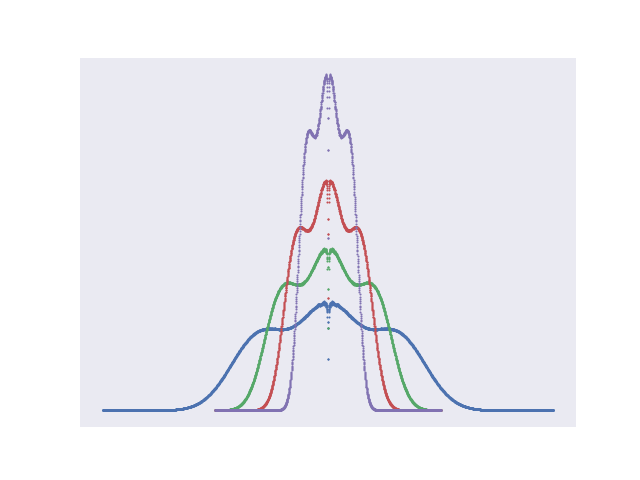
\includegraphics[scale=0.7]{Images/art.png}
	\caption{One-body density plots for a two-dimensional single quantum dot with 12 electrons. The four graphs correspond to four different oscillator strengths, where the weakest oscillator gives the broadest density distribution. It's quite artistic, isn't it?}
\end{figure}
After all, this thesis is related to a master in physics, and therefore the results and the physical insight is the interesting part. Before we move on to the physical results, we will take a quick look at some more technical results, more precisely the computational cost of various wave function structures and the energy convergence using various optimization tools. 

For validation purposes, we will present a few selected results on the case without repulsive interaction and compare to analytical results. Thereafter, we study the case with repulsive interaction in a much larger scale, where we compare various wave function structures for different number of particles and oscillator strengths in two and three dimensions.

\newpage
\section{Computational cost}
One of the major problems of quantum many-body simulations is the computational cost, which explodes as the system size increases. In figure \eqref{fig:cpu_time} the CPU-time is plotted as a function of number of particles. 
\begin{figure}[H]
	\centering
	% This file was created by matplotlib2tikz v0.7.4.
\begin{tikzpicture}[scale=0.9]

\begin{axis}[name=2D, xlabel=$N$, ylabel={CPU-time [s]}, grid=major, 
legend cell align={left},
legend style={at={(1.68,1.10)}, anchor=south east, draw=white!80.0!black},
legend columns = 6, 
clip=false,
xtick=data] 
\addplot[color=color0,mark=oplus*, dashed] coordinates { 
	(2,6.05)
	(6,11.25)
	(12,20.53) 
	(20,38.99) 
	(30,73.73) 
	(42,130.49) 
	(56,213.47)
	(72,360.22)
	(90,856.84) }; 
\addlegendentry{RBM};

\addplot[color=color1,mark=oplus*, dash dot] coordinates { 
	(2,7.12) 
	(6,14.07) 
	(12,28.42) 
	(20,63.27) 
	(30,122.93) 
	(42,199.60)
	(56,349.22)}; 
\addlegendentry{RBM+SJ};

\addplot[color=color2,mark=oplus*, dotted] coordinates { 
	(2,7.26)
	(6,13.50)
	(12,27.68)
	(20,57.09) 
	(30,119.17) 
	(42,212.53) 
	(56,382.13) }; 
\addlegendentry{RBM+PJ};

\addplot[color=color3,mark=oplus*] coordinates { 
	(2,5.11)
	(6,10.51)
	(12,20.85) 
	(20,41.20) 
	(30,76.26) 
	(42,137.39) 
	(56,230.63)
	(72,355.81)
	(90,544.03) }; 
\addlegendentry{VMC};

\node[] at (axis cs: 44,978) {2D};
\end{axis}

\begin{axis}[name=2D, 
xshift=7.9cm, 
xlabel=$N$, 
grid=major, 
clip=false,
xtick=data] 
\addplot[color=color0,mark=oplus*, dashed] coordinates { 
	(2,7.69)
	(8,20.92)
	(20,59.67) 
	(40,171.84) 
	(70,586.39) }; 
%\addlegendentry{RBM};

\addplot[color=color1,mark=oplus*, dash dot] coordinates { 
	(2,8.95)
	(8,26.86)
	(20,94.64) 
	(40,270.92) }; 
%\addlegendentry{RBM+SJ};

\addplot[color=color2,mark=oplus*, dotted] coordinates { 
	(2,8.87)
	(8,26.36)
	(20,91.40) 
	(40,293.25) }; 
%\addlegendentry{RBM+PJ};

\addplot[color=color3,mark=oplus*] coordinates { 
	(2,6.70)
	(8,20.99)
	(20,62.54) 
	(40,185.65) 
	(70,486.02) };
%\addlegendentry{VMC};

\node[] at (axis cs: 35,670) {3D};
\end{axis}
\end{tikzpicture}
	\label{fig:cpu_time}
	\caption{CPU-time as a function of number of particles for two and three dimensions. The solid line is restricted Boltzmann machine (RBM), while the dashed line is a standard variational Monte-Carlo wave function (VMC).}
\end{figure}

\iffalse
\begin{figure}[H]
	\centering
	\label{fig:cpu_time2}
	\subfloat[2D]{{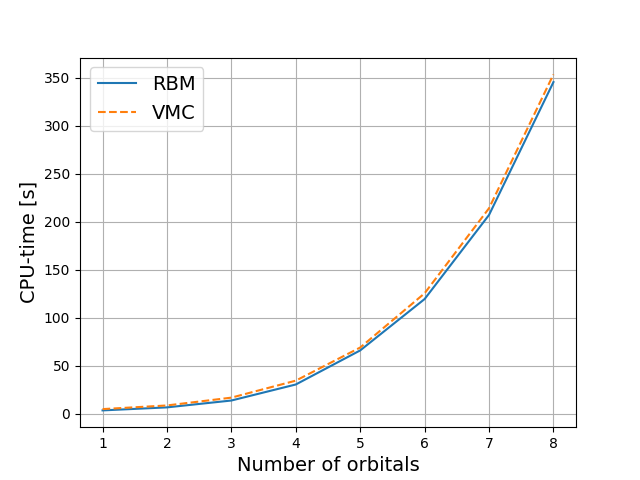
\includegraphics[width=8cm]{/home/evenmn/VMC/plots/cpu_time_2D.png}}}
	\subfloat[3D]{{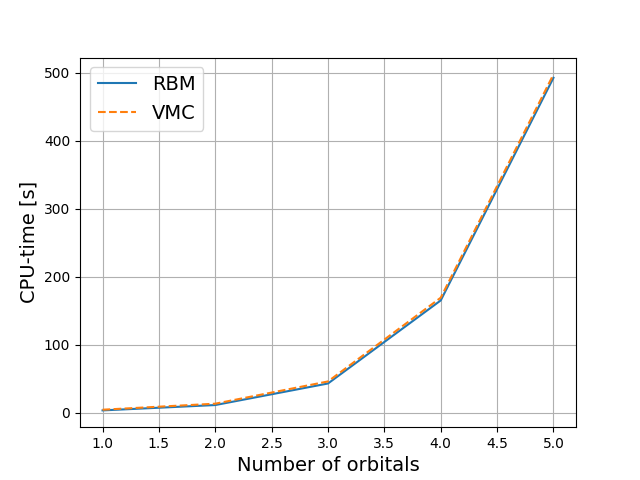
\includegraphics[width=8cm]{/home/evenmn/VMC/plots/cpu_time_3D.png}}}
	\caption{CPU-time as a function of full orbitals for two and three dimensions. The solid line is RBM, while the dashed line is VMC.}
\end{figure}

% This file was created by matplotlib2tikz v0.7.4.
\begin{tikzpicture}[scale=0.9]

\begin{axis}[name=2D, xlabel=$N$, ylabel={CPU-time [s]}, grid=major, legend pos=north west, xtick=data] 
\addplot[color=color1,mark=oplus*, dashed] coordinates { 
	(2,6.05)
	(6,11.25)
	(12,20.53) 
	(20,38.99) 
	(30,73.73) 
	(42,130.49) 
	(56,213.47)
	(72,360.22)
	(90,856.84) }; 
\addlegendentry{RBM};

\addplot[color=color2,mark=oplus*, dash dot] coordinates { 
	(2,7.12) 
	(6,14.07) 
	(12,28.42) 
	(20,63.27) 
	(30,122.93) 
	(42,199.60)
	(56,349.22)}; 
\addlegendentry{RBM+SJ};

\addplot[color=color3,mark=oplus*, dotted] coordinates { 
	(2,7.26)
	(6,13.50)
	(12,27.68)
	(20,57.09) 
	(30,119.17) 
	(42,212.53) 
	(56,382.13) }; 
\addlegendentry{RBM+PJ};

\addplot[color=color0,mark=oplus*] coordinates { 
	(2,5.11)
	(6,10.51)
	(12,20.85) 
	(20,41.20) 
	(30,76.26) 
	(42,137.39) 
	(56,230.63)
	(72,355.81)
	(90,544.03) }; 
\addlegendentry{VMC};
\end{axis}
\end{tikzpicture}
\fi

As the applied theory used in quantum many-body simulations agrees perfectly with laboratory experiments, they can be considered as actual experiments. In that manner, one can use computer experiments to verify other experiments and even predict new thing. Similarly to experiments in a laboratory, computer experiments are also dependent on external factors, especially when it comes to the CPU-time, and therefore it is important to do such measurements multiple times to find an accurate average time. The CPU-times above are the average from at least four independent runs for each number of orbitals. All the runs were performed on the Abel computational cluster, which is equipped with Supermicro X9DRT compute nodes with dual Intel E5-2670 CPUs running at 2.6 GHz. Different hardware might give different CPU-times, but the CPU-time ratios (the exponential factor) should be the same. 

To estimate how fast the cost increases as we add more particles, we do regression with a function on the form $f(x)=ax^b$ where $x$ is the number of particles while $a$ and $b$ are parameters to find. From the limited number of points, we have found the parameters and presented them in table \eqref{tab:cputimefit}.

\begin{table} [H]
	\caption{Constants $a$ and $b$ for restricted Boltzmann machine (RBM), restricted Boltzmann machine with a simple Jastrow factor (RBM+SJ), restricted Boltzmann machine with Padé-Jastrow factor (RBM+PJ) and standard variational Monte-Carlo sampling (VMC).}
	\begin{tabularx}{\textwidth}{X|CC:CC} \hline\hline
		\label{tab:cputimefit}
		& \multicolumn{2}{c}{2D} &
		\multicolumn{2}{c}{3D} \\ \hline
		& $a$ & $b$ & $a$ & $b$ \\ \hline \\
		RBM & 0.0840 & 1.92 & 0.0302 & 2.268 \\ 
		RBM+SJ & - & - & - & - \\
		RBM+PJ & - & - & - & - \\
		VMC & 0.111 & 1.88 & 0.148 & 1.91 \\ \hline\hline
	\end{tabularx}
\end{table}

\section{Energy convergence}
Another important thing is the convergence. We want our calculations to converge fast and to be stable, and that is what the optimization tools are responsible for. In figure \eqref{fig:convergenceoptimization} we compare standard gradient descent to stochastic gradient descent and ADAM for two interacting electrons in a two- and three dimensional well. 

\begin{figure} [H]
	\centering
	\begin{tikzpicture} [scale=0.9, spy using outlines=
	{rectangle, magnification=8,size=2cm, height=1cm, connect spies}]
	\begin{axis} [name=2D, xlabel=Iteration, ylabel={Energy [Ha]}, grid=major, every axis plot/.append style={thick}]
		\addplot table [x expr=\coordindex+1, y index=0, mark=none] {/home/evenmn/VMC/data/int1/energy/VMC/2D/2P/1.000000w/GD_MC16777216.dat};
		\addlegendentry{GD};
		
		\addplot table [x expr=\coordindex+1, y index=0, mark=none, green] {/home/evenmn/VMC/data/int1/energy/VMC/2D/2P/1.000000w/ADAM_MC16777216.dat}; 
		\addlegendentry{ADAM};
		
		\addplot+ [dashed,mark=none,black] coordinates {(0,3) (100,3)};
		\addlegendentry{Exact};
		
		\coordinate (spypoint1) at (axis cs:75,2.995);
		\coordinate (magnifyglass1) at (axis cs:50,3.05);
	\end{axis}
	\spy [size=2.0cm] on (spypoint1)
	in node[fill=white] at (magnifyglass1);
	
	\begin{axis} [name=3D, at=(2D.right of south east), anchor=left of south west, xlabel=Iteration, grid=major, every axis plot/.append style={thick}]	
		\addplot table [x expr=\coordindex+1, y index=0, mark=none] {/home/evenmn/VMC/data/int1/energy/VMC/3D/2P/0.500000w/GD_MC16777216.dat};  
		\addlegendentry{GD};
		
		\addplot table [x expr=\coordindex+1, y index=0, mark=none] {/home/evenmn/VMC/data/int1/energy/VMC/3D/2P/0.500000w/ADAM_MC16777216.dat}; 
		\addlegendentry{ADAM};
		
		\addplot+ [dashed,mark=none,color=black] coordinates {(0,2) (100,2)};
		\addlegendentry{Exact};
		
		\coordinate (spypoint2) at (axis cs:75,1.997);
		\coordinate (magnifyglass2) at (axis cs:50,2.04);
	\end{axis} 
	\spy [size=2.0cm] on (spypoint2)
	in node[fill=white] at (magnifyglass2);
\end{tikzpicture}
	\caption{Energy convergence for two electrons in a two dimensional (a) and three dimensional (b) quantum dot. We use standard variational Monte-Carlo wave function, the learning rate was set to $\eta=0.5$ and the number of Metropolis steps used for each iteration was $M=2^{24}$.}
\end{figure}

We observe that the gradient descent methods in the cases above have a smoother convergence compared ADAM. However, this could be the case for the standard variational Monte-Carlo wave function only, so we better also look how well they do for other structures. 
\iffalse
\begin{figure}[H]
	\centering
	\label{fig:convergenceoptimization2}
	\subfloat[2D, 2P, $\omega=1$]{{\includegraphics[width=8cm]{/home/evenmn/VMC/plots/int1/energy/2D/2P/1.000000w/MC2pow24.png}}}
	\subfloat[3D, 2P, $\omega=1/2$]{{\includegraphics[width=8cm]{/home/evenmn/VMC/plots/int1/energy/3D/2P/0.500000w/MC2pow24.png}}}
	\caption{Energy convergence for two electrons in a two dimensional (a) and three dimensional (b) quantum dot. The learning rate was set to $\eta=0.5$, and the number of Metropolis steps used for each iteration was $MC=2^{24}$.}
\end{figure}
\fi

\begin{figure}[H]
	\centering
	
\includegraphics[scale=0.3]{Images/example.png}
	\caption{Will add convergence plots here}
\end{figure}

Even though the gradient descent methods seem to be the best choice based on those graphs, we experience that the energy occasionally explode when they are applied on more heavy systems, and therefore we will rely in the ADAM optimizer henceforth. 

\section{No repulsive interaction}
We start with the non-interacting case in order to validate the implemented code. In this case we both know the exact energies and the exact one-body densities for an array of systems, and can therefore testify the flexibility of the code. 

\subsection{Ground state energy}
\subsubsection{Quantum dots}
The single quantum dot has analytical ground-state energies given by equation \eqref{eq:HOenergies} and number of closed-shell particles given by equation \eqref{eq:HOclosedshell}. The first 5 closed-shell energies for $\omega=0.5$ and $\omega=1.0$ are presented in table \eqref{tab:quantumdotswointeraction}.

\begin{table} [H]
	\caption{Energy of $N$ non-interacting electrons trapped in a harmonic oscillator of frequency $\omega=0.5$ and $\omega=1.0$. $E_{\text{RBM}}$ is a single Slater determinant with a plain Boltzmann machine baked in, while $E_{\text{VMC}}$ is standard variational Monte-Carlo.}
	\label{tab:quantumdotswointeraction}
	\begin{tabularx}{\textwidth}{r|r|XXX:XXX} \hline\hline
		\label{tab:nn}
		& $\omega$ & \multicolumn{3}{c}{0.5}&\multicolumn{3}{c}{1.0}\\ \hline
		& $N$ & $E_{\text{RBM}}$ & $E_{\text{VMC}}$ & $E_{\text{exact}}$ & $E_{\text{RBM}}$ & $E_{\text{VMC}}$ & $E_{\text{exact}}$ \\ \hline
		
		\parbox[t]{2mm}{\multirow{5}{*}{\rotatebox[origin=c]{90}{2D}}}
		&2 & 1.00045(5) & 1.0 & 1 & 2.00098(5) & 2.0 & 2\\
		&6 & 5.009(2) & 5.0 & 5 & 10.010(1) & 10.0 & 10 \\
		&12 & - & 14.0 & 14 & - & 28.0 & 28\\
		&20 & - & 30.0 & 30 & - & 60.0 & 60\\
		&30 & - & 55.0 & 55 & - & 110.0 & 110\\ \hline
		
		\parbox[t]{2mm}{\multirow{5}{*}{\rotatebox[origin=c]{90}{3D}}}
		&2 & 1.5050(3) & 1.5 & 1.5 & 3.0063(2) & 3.0 & 3 \\
		&8 & - & 9.0 & 9 & - & 18.0 & 18 \\
		&20 & - & 30.0 & 30 & - & 60.0 & 60 \\
		&40 & - & 75.0 & 75 & - & 150.0 & 150 \\
		&70 & - & 157.5 & 157.5 & - & 315.0 & 315 \\ \hline\hline
	\end{tabularx}
\end{table}
We observe that the restricted Boltzmann machine wave function is able to reproduce the exact energy for most of the cases, but when the number of particles get large, the statistical error gets significant.

\subsection{One-body density}
We will also focus on the one-body densities throughout the results, and comparing the obtained densities to the analytical ones is a good indicator on whether the implementation is correct or not. The analytical one-body densities are found from the definition of one-body density in equation \eqref{eq:electron_density}.

\begin{figure} [h]%
	\centering
	\subfloat[2D, $\omega=0.5$]{{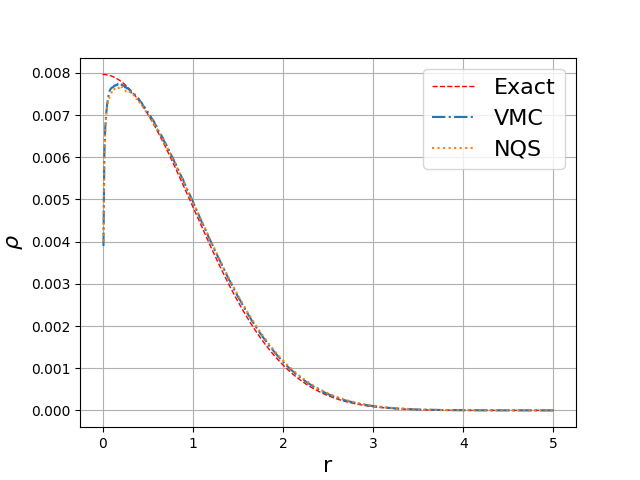
\includegraphics[width=8cm]{/home/evenmn/VMC/plots/int0/onebody/2D/2P/onebody_VMC_NQS_P2_D2_w0p5.png}}}
	\subfloat[2D, $\omega=1.0$]{{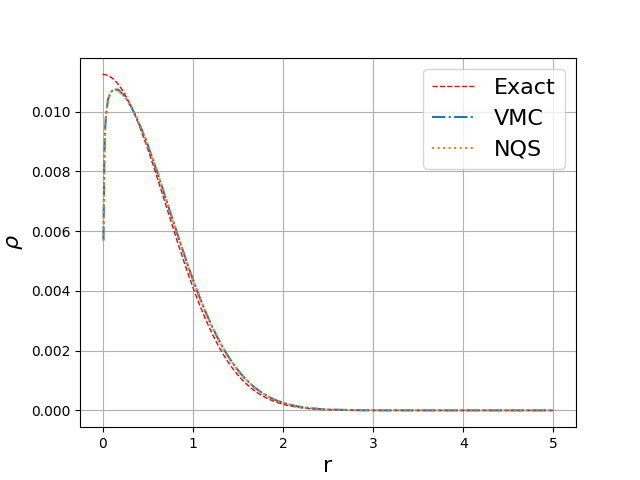
\includegraphics[width=8cm]{/home/evenmn/VMC/plots/int0/onebody/2D/2P/onebody_VMC_NQS_P2_D2_w1p0.png} }}\\
	
	\subfloat[3D, $\omega=0.5$]{{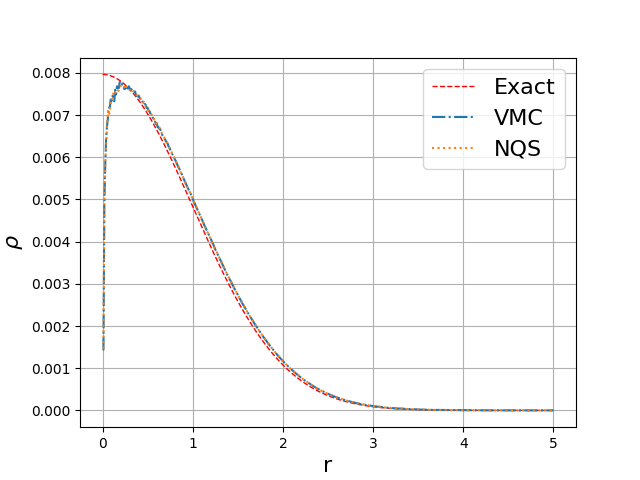
\includegraphics[width=8cm]{/home/evenmn/VMC/plots/int0/onebody/3D/2P/onebody_VMC_NQS_P2_D3_w0p5.png} }}
	\subfloat[3D, $\omega=1.0$]{{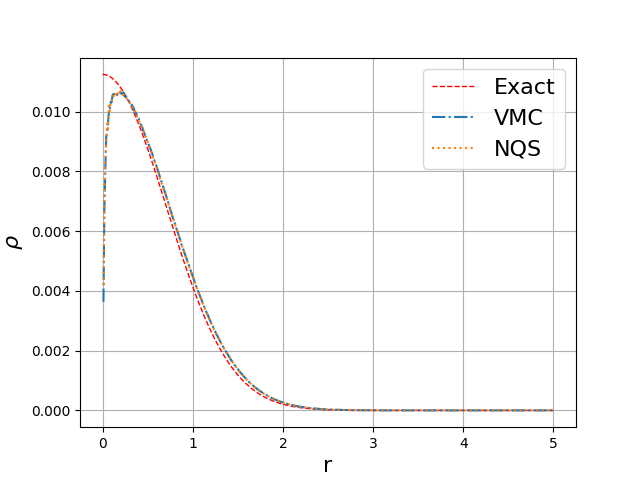
\includegraphics[width=8cm]{/home/evenmn/VMC/plots/int0/onebody/3D/2P/onebody_VMC_NQS_P2_D3_w1p0.png} }}
	\caption{One-body densities of two non-interacting electrons in two dimensions figure (a) and (b) and three dimensions}%
	\label{fig:OB_nointeraction1}
\end{figure}

We observe that both the standard variational Monte-Carlo wave function and the restricted Boltzmann machine reproduce the analytical one-body density. The distribution gets narrower when the frequency is increased. 

\iffalse
\begin{figure} [H]
	\centering
	% This file was created by matplotlib2tikz v0.7.4.
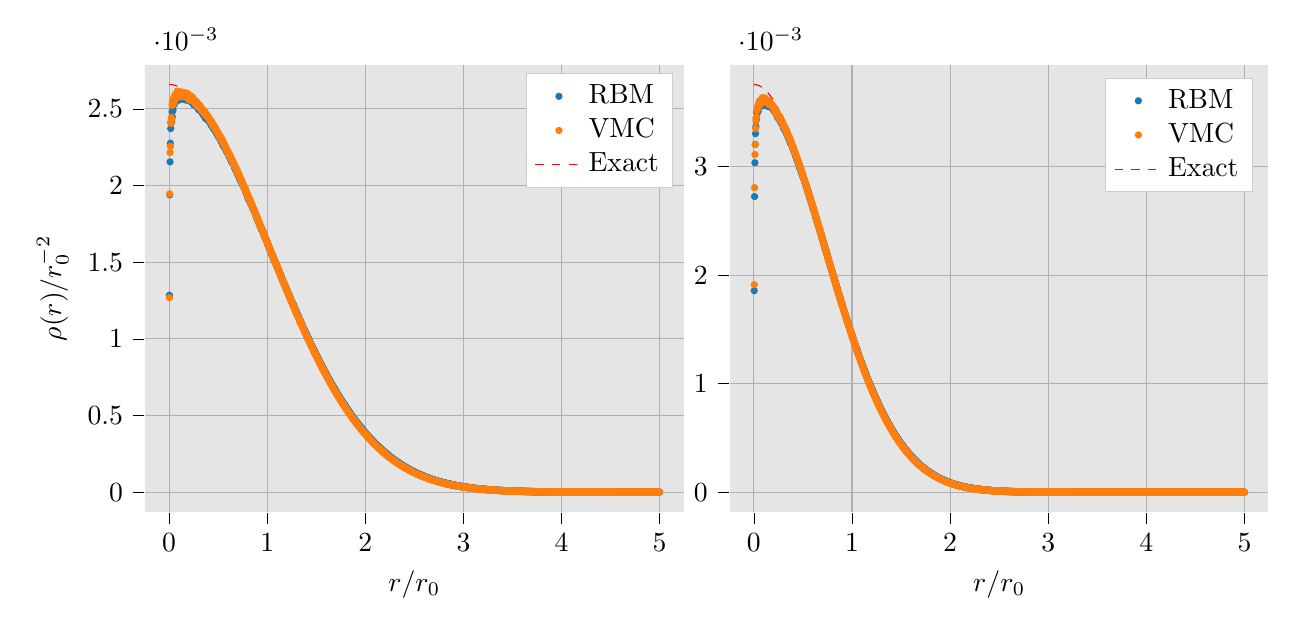
\begin{tikzpicture}

\definecolor{color0}{rgb}{0.12156862745098,0.466666666666667,0.705882352941177}
\definecolor{color1}{rgb}{1,0.498039215686275,0.0549019607843137}

%\definecolor{color0}{rgb}{0.886274509803922,0.290196078431373,0.2}
%\definecolor{color1}{rgb}{0.203921568627451,0.541176470588235,0.741176470588235}

\begin{axis}[
name=2D05,
axis line style={white},
axis background/.style={fill=white!89.80392156862746!black},
legend cell align={left},
legend style={draw=white!80.0!black},
tick align=outside,
tick pos=left,
x grid style={white!69.01960784313725!black},
xlabel={\(\displaystyle r / r_0\)},
xmajorgrids,
xmin=-0.25, xmax=5.25,
xtick style={color=black},
y grid style={white!69.01960784313725!black},
ylabel={\(\displaystyle \rho(r) / r_0^{-2}\)},
ymajorgrids,
ymin=-0.000132883773143863, ymax=0.00279074646387709,
ytick style={color=black}
]
\addplot [semithick, color0, opacity=1.0, mark=*, mark size=1, mark options={solid}, only marks]
table {%
0 nan
0.00333555703802535 0.00128411356068203
0.0066711140760507 0.00193901606438821
0.0100066711140761 0.00215395254283749
0.0133422281521014 0.00227529875105485
0.0166777851901268 0.00237132053320946
0.0200133422281521 0.00241591354431996
0.0233488992661775 0.00243092206804763
0.0266844563042028 0.0024135623181683
0.0300200133422282 0.00247891875892053
0.0333555703802535 0.00244770670964875
0.0366911274182789 0.002493029591405
0.0400266844563042 0.00248935590915473
0.0433622414943296 0.00254966434529242
0.0466977985323549 0.00252556096875834
0.0500333555703803 0.00254690933758901
0.0533689126084056 0.0025296039307996
0.056704469646431 0.00255597510790233
0.0600400266844563 0.00255971428088
0.0633755837224817 0.00255620236528163
0.066711140760507 0.00254446253313851
0.0700466977985324 0.00254974500917541
0.0733822548365577 0.00256530763878107
0.0767178118745831 0.00256687074063606
0.0800533689126084 0.00257048276921687
0.0833889259506338 0.00255758352200435
0.0867244829886591 0.0025600044467924
0.0900600400266845 0.00258487898498557
0.0933955970647098 0.0025619189536401
0.0967311541027352 0.00257490310074842
0.100066711140761 0.00256877765236543
0.103402268178786 0.00255779367093498
0.106737825216811 0.00257962483350168
0.110073382254837 0.0025764572817885
0.113408939292862 0.00258687500969459
0.116744496330887 0.00256749308002891
0.120080053368913 0.00258295892315983
0.123415610406938 0.00257705545634089
0.126751167444963 0.00257786141388794
0.130086724482989 0.0025728266431917
0.133422281521014 0.0025701654492647
0.136757838559039 0.0025630015527129
0.140093395597065 0.0025766817045993
0.14342895263509 0.00257381778502133
0.146764509673115 0.00257266890557961
0.150100066711141 0.0025695626687933
0.153435623749166 0.00258346645777864
0.156771180787191 0.00258383526092402
0.160106737825217 0.00257866427159826
0.163442294863242 0.00256909785917234
0.166777851901268 0.00255947367844237
0.170113408939293 0.00256905471698703
0.173448965977318 0.00255700475864395
0.176784523015344 0.00255795227390149
0.180120080053369 0.0025638007841463
0.183455637091394 0.00256319726994251
0.18679119412942 0.002560706474649
0.190126751167445 0.00256062914964933
0.19346230820547 0.00256339415524576
0.196797865243496 0.00256953346611306
0.200133422281521 0.00256779893058522
0.203468979319546 0.00255811901117508
0.206804536357572 0.00255614355785294
0.210140093395597 0.0025680596317737
0.213475650433622 0.00255076496616454
0.216811207471648 0.00255347571376341
0.220146764509673 0.00254715818872347
0.223482321547698 0.00254852030268339
0.226817878585724 0.0025559008941644
0.230153435623749 0.00254687077382322
0.233488992661775 0.00254248324310979
0.2368245496998 0.00254811206259356
0.240160106737825 0.00254821939747189
0.243495663775851 0.00253983329643069
0.246831220813876 0.0025499628834134
0.250166777851901 0.00252875404856625
0.253502334889927 0.00253221321835815
0.256837891927952 0.0025231538851593
0.260173448965977 0.00252496103112864
0.263509006004003 0.00252643206211492
0.266844563042028 0.00252337604884667
0.270180120080053 0.00252207767075588
0.273515677118079 0.00252562810668533
0.276851234156104 0.00251834215864005
0.280186791194129 0.00251605775504431
0.283522348232155 0.00251548409248827
0.28685790527018 0.00251279526443407
0.290193462308205 0.00251255704682956
0.293529019346231 0.00251777741965761
0.296864576384256 0.00249941590097819
0.300200133422282 0.00251000337046052
0.303535690460307 0.00249384493826766
0.306871247498332 0.00250262217703483
0.310206804536358 0.00250065388071274
0.313542361574383 0.00249061103524088
0.316877918612408 0.002500009569388
0.320213475650434 0.00249593647503041
0.323549032688459 0.00248603057262945
0.326884589726484 0.00248235645675502
0.33022014676451 0.00248367334484141
0.333555703802535 0.00248472991949049
0.33689126084056 0.00248423480497606
0.340226817878586 0.0024751630940011
0.343562374916611 0.00246729643778062
0.346897931954636 0.00246156615115585
0.350233488992662 0.00247108024609159
0.353569046030687 0.0024710142532694
0.356904603068712 0.00246962033032532
0.360240160106738 0.0024630357696142
0.363575717144763 0.00244933683699453
0.366911274182789 0.00244943337506212
0.370246831220814 0.00243726521964314
0.373582388258839 0.00244781484966687
0.376917945296865 0.00243763028713926
0.38025350233489 0.00244567763266857
0.383589059372915 0.00244075126906267
0.386924616410941 0.00243645958276886
0.390260173448966 0.00243211186032164
0.393595730486991 0.00243520934488331
0.396931287525017 0.0024345652879096
0.400266844563042 0.0024233189509147
0.403602401601067 0.0024201297321541
0.406937958639093 0.00242549895089426
0.410273515677118 0.00241810671660182
0.413609072715143 0.00241378985618298
0.416944629753169 0.00241855242291984
0.420280186791194 0.00240880615996373
0.423615743829219 0.00240273186699727
0.426951300867245 0.00239760193698943
0.43028685790527 0.00239154507906578
0.433622414943296 0.0023961579510787
0.436957971981321 0.00239598656341817
0.440293529019346 0.00239558838462313
0.443629086057372 0.00238778679128034
0.446964643095397 0.00238596301446963
0.450300200133422 0.00237167396051898
0.453635757171448 0.00237410759640387
0.456971314209473 0.00237622441154521
0.460306871247498 0.00237453063426573
0.463642428285524 0.00236671231148222
0.466977985323549 0.00236796163870709
0.470313542361574 0.00235430092586941
0.4736490993996 0.00235179800604489
0.476984656437625 0.00235470386497831
0.48032021347565 0.00235030541404743
0.483655770513676 0.00234782171857077
0.486991327551701 0.0023360299877179
0.490326884589726 0.00233688862660146
0.493662441627752 0.00233397246047953
0.496997998665777 0.00233335236831001
0.500333555703803 0.00232243338028832
0.503669112741828 0.00231974379936311
0.507004669779853 0.00232002335839156
0.510340226817879 0.00231563953987214
0.513675783855904 0.00230849445964902
0.517011340893929 0.00230863399515627
0.520346897931955 0.00230783948572416
0.52368245496998 0.00230262805673563
0.527018012008005 0.00229266254529619
0.530353569046031 0.00229013106034475
0.533689126084056 0.0022885028930407
0.537024683122081 0.00228587766587144
0.540360240160107 0.0022809881377922
0.543695797198132 0.00228044520267037
0.547031354236157 0.00226643934210505
0.550366911274183 0.00226190110645852
0.553702468312208 0.00226937888456428
0.557038025350234 0.00226324833070813
0.560373582388259 0.00225727541470067
0.563709139426284 0.00225150077263543
0.56704469646431 0.00224759408801561
0.570380253502335 0.00224512283761507
0.57371581054036 0.00223879139729675
0.577051367578386 0.00224103243923343
0.580386924616411 0.00223510840596963
0.583722481654436 0.00222803828616393
0.587058038692462 0.00222081912071152
0.590393595730487 0.00221890690674609
0.593729152768512 0.00222001368560887
0.597064709806538 0.00221460322075315
0.600400266844563 0.0022105501882833
0.603735823882588 0.00220086680759002
0.607071380920614 0.00219947722179645
0.610406937958639 0.00219745853098719
0.613742494996664 0.00219045763518791
0.61707805203469 0.0021824313627459
0.620413609072715 0.00217902735538171
0.62374916611074 0.00217860622391017
0.627084723148766 0.00217415088103914
0.630420280186791 0.00217054129443944
0.633755837224817 0.00215710119382775
0.637091394262842 0.00216015442348986
0.640426951300867 0.00215372554437773
0.643762508338893 0.00214770320776587
0.647098065376918 0.0021497928176167
0.650433622414943 0.00214924244427026
0.653769179452969 0.00214778715738854
0.657104736490994 0.00213742729755119
0.660440293529019 0.00213068936416032
0.663775850567045 0.00212842939076001
0.66711140760507 0.00211823684412399
0.670446964643095 0.00211600424918624
0.673782521681121 0.00211089802058971
0.677118078719146 0.00210130406086795
0.680453635757171 0.00210835157423184
0.683789192795197 0.0021000385495291
0.687124749833222 0.0020947459624521
0.690460306871247 0.00208571019153715
0.693795863909273 0.00208582653707172
0.697131420947298 0.00207785282690729
0.700466977985324 0.00207705078974613
0.703802535023349 0.00206563275896935
0.707138092061374 0.00207375982539428
0.7104736490994 0.00206443740818688
0.713809206137425 0.00205519139731239
0.71714476317545 0.00205309867753331
0.720480320213476 0.00204068163889168
0.723815877251501 0.00204243195992289
0.727151434289526 0.00203224646917199
0.730486991327552 0.00203417434243794
0.733822548365577 0.00203245827514628
0.737158105403602 0.00202576932914127
0.740493662441628 0.00202261246103681
0.743829219479653 0.00201017672235416
0.747164776517678 0.00201357123370242
0.750500333555704 0.0020050869210649
0.753835890593729 0.00200064630480642
0.757171447631754 0.0019959962251333
0.76050700466978 0.0019942080045798
0.763842561707805 0.00198603257386971
0.767178118745831 0.00198405787794548
0.770513675783856 0.00197997719944462
0.773849232821881 0.00197887814745394
0.777184789859907 0.00196675821940867
0.780520346897932 0.00195811800009438
0.783855903935957 0.00195544902433141
0.787191460973983 0.0019540079255553
0.790527018012008 0.00194327764666495
0.793862575050033 0.00194331467829942
0.797198132088059 0.00193751592499642
0.800533689126084 0.00192890196880412
0.803869246164109 0.0019218995377673
0.807204803202135 0.00191206014046122
0.81054036024016 0.00191829846513077
0.813875917278185 0.00190578866050806
0.817211474316211 0.00190833519638872
0.820547031354236 0.00190271682519257
0.823882588392261 0.00190262325340566
0.827218145430287 0.00189065406180533
0.830553702468312 0.00188377779569209
0.833889259506338 0.0018804707625998
0.837224816544363 0.00187742952114297
0.840560373582388 0.00187336196550528
0.843895930620414 0.00186591385251899
0.847231487658439 0.00186323857872143
0.850567044696464 0.00186408357765188
0.85390260173449 0.00185464611317328
0.857238158772515 0.00184489293584272
0.86057371581054 0.00184159554939874
0.863909272848566 0.00183867612111673
0.867244829886591 0.00183683962796194
0.870580386924616 0.00183122044202499
0.873915943962642 0.00182347109410825
0.877251501000667 0.00182244252036519
0.880587058038692 0.00181397532047356
0.883922615076718 0.00180817233078253
0.887258172114743 0.00180555368986576
0.890593729152768 0.00179202995728709
0.893929286190794 0.00179005600174608
0.897264843228819 0.0017868193131607
0.900600400266845 0.0017763018692597
0.90393595730487 0.00178034480230222
0.907271514342895 0.00176974970825492
0.910607071380921 0.00176850185849712
0.913942628418946 0.00175688038373919
0.917278185456971 0.00175892152522224
0.920613742494997 0.00174927402551525
0.923949299533022 0.00174021955166786
0.927284856571047 0.00173737418350185
0.930620413609073 0.00173692037623061
0.933955970647098 0.00173079737494367
0.937291527685123 0.00172738897603314
0.940627084723149 0.00171136726547599
0.943962641761174 0.00171877853654417
0.947298198799199 0.00171007561513252
0.950633755837225 0.00170935690600187
0.95396931287525 0.00169956716102096
0.957304869913275 0.00169775352594629
0.960640426951301 0.00169085975520268
0.963975983989326 0.00168195475706869
0.967311541027352 0.00168486216201991
0.970647098065377 0.00167374352118648
0.973982655103402 0.00166556209979221
0.977318212141428 0.00166607654152899
0.980653769179453 0.00165406009454944
0.983989326217478 0.00165421969014153
0.987324883255504 0.00164692774982996
0.990660440293529 0.00164089286872101
0.993995997331554 0.00163866414685143
0.99733155436958 0.00163258372712525
1.00066711140761 0.00162779477230589
1.00400266844563 0.00161770151088574
1.00733822548366 0.00161805375616737
1.01067378252168 0.00161042279381186
1.01400933955971 0.00160755957876971
1.01734489659773 0.00159756726098882
1.02068045363576 0.00159468680940915
1.02401601067378 0.00158695044294712
1.02735156771181 0.0015859925283592
1.03068712474983 0.00157467307389125
1.03402268178786 0.00156987762836327
1.03735823882588 0.00157124822652217
1.04069379586391 0.00155871736544904
1.04402935290193 0.00155241534254763
1.04736490993996 0.00155238638256231
1.05070046697799 0.00154948989337667
1.05403602401601 0.00154415815678001
1.05737158105404 0.00153426216985868
1.06070713809206 0.00153571315322373
1.06404269513009 0.00152734960490807
1.06737825216811 0.00151913008393628
1.07071380920614 0.0015090723616834
1.07404936624416 0.00150892226819045
1.07738492328219 0.00150993211670343
1.08072048032021 0.00150315070214559
1.08405603735824 0.00150023368078424
1.08739159439626 0.00149521517977876
1.09072715143429 0.00148767534470328
1.09406270847231 0.00147927372351066
1.09739826551034 0.00147321008289833
1.10073382254837 0.00146702887611509
1.10406937958639 0.00146717620687332
1.10740493662442 0.0014597583762478
1.11074049366244 0.00145246638176487
1.11407605070047 0.00145393067203348
1.11741160773849 0.00144636682431295
1.12074716477652 0.00144124018777526
1.12408272181454 0.00143482482568705
1.12741827885257 0.00143345052410189
1.13075383589059 0.00142607152508493
1.13408939292862 0.00142200133641342
1.13742494996664 0.0014186613462476
1.14076050700467 0.00140716072725643
1.1440960640427 0.00140351966875975
1.14743162108072 0.00139931030560654
1.15076717811875 0.00139142854218226
1.15410273515677 0.0013860559377964
1.1574382921948 0.00138325277090608
1.16077384923282 0.0013769919373777
1.16410940627085 0.00137314630707983
1.16744496330887 0.00136353290078121
1.1707805203469 0.00136001285963317
1.17411607738492 0.00135732870983363
1.17745163442295 0.00135143274106131
1.18078719146097 0.00134676626955668
1.184122748499 0.00134670996939818
1.18745830553702 0.00133869757541467
1.19079386257505 0.00133114900694938
1.19412941961308 0.00132482286775917
1.1974649766511 0.00132125395644027
1.20080053368913 0.00131785524892999
1.20413609072715 0.00131114320950016
1.20747164776518 0.00130831715429173
1.2108072048032 0.00130283237303558
1.21414276184123 0.00129635178417847
1.21747831887925 0.00129102536428135
1.22081387591728 0.00128893446740163
1.2241494329553 0.00128438607602785
1.22748498999333 0.00127841626295505
1.23082054703135 0.00127152519937035
1.23415610406938 0.00126538062741939
1.2374916611074 0.00126201688848217
1.24082721814543 0.00125559546284255
1.24416277518346 0.00125017152870337
1.24749833222148 0.00124720050610749
1.25083388925951 0.00124275400165288
1.25416944629753 0.00123552358712856
1.25750500333556 0.00123354113063187
1.26084056037358 0.00122769020150562
1.26417611741161 0.00122322589716264
1.26751167444963 0.00122266174495958
1.27084723148766 0.00121234343978459
1.27418278852568 0.00121051246581378
1.27751834556371 0.001202966536843
1.28085390260173 0.00119862116182001
1.28418945963976 0.00119271588145122
1.28752501667779 0.00119033787845484
1.29086057371581 0.00118164058417703
1.29419613075384 0.00118131466622626
1.29753168779186 0.00117398849045199
1.30086724482989 0.00116812091354845
1.30420280186791 0.00116444464160885
1.30753835890594 0.00115534267416396
1.31087391594396 0.00115761166932742
1.31420947298199 0.00114973998181479
1.31754503002001 0.00114590937309906
1.32088058705804 0.00114107976756244
1.32421614409606 0.00113549330244641
1.32755170113409 0.00112914761380096
1.33088725817211 0.00112397319891302
1.33422281521014 0.00111957246070972
1.33755837224817 0.00111638694612675
1.34089392928619 0.0011089673266224
1.34422948632422 0.00110647054860825
1.34756504336224 0.00110214534962468
1.35090060040027 0.00109602906190732
1.35423615743829 0.00109332609296788
1.35757171447632 0.00108393286862374
1.36090727151434 0.00108263675561169
1.36424282855237 0.00107578670718291
1.36757838559039 0.00107040234940042
1.37091394262842 0.00107076270528109
1.37424949966644 0.00106210168987299
1.37758505670447 0.00105922564563929
1.38092061374249 0.001052855079175
1.38425617078052 0.00104713649620926
1.38759172781855 0.00104647980951826
1.39092728485657 0.00104423650961999
1.3942628418946 0.00103748972070886
1.39759839893262 0.00102553698904287
1.40093395597065 0.001029416509912
1.40426951300867 0.00102484636884994
1.4076050700467 0.00101999566048963
1.41094062708472 0.00100980682557362
1.41427618412275 0.00100704217116094
1.41761174116077 0.00100599069615559
1.4209472981988 0.00099825098438681
1.42428285523682 0.000997844960887959
1.42761841227485 0.000991553926090246
1.43095396931288 0.000984831305476541
1.4342895263509 0.000979980390806297
1.43762508338893 0.000973899134308139
1.44096064042695 0.000969287140125657
1.44429619746498 0.000966830338827675
1.447631754503 0.000963990565677937
1.45096731154103 0.0009580758129948
1.45430286857905 0.000951889356569407
1.45763842561708 0.000950756751019208
1.4609739826551 0.000945334840194517
1.46430953969313 0.000942715366703929
1.46764509673115 0.000937247749652044
1.47098065376918 0.000929990631871786
1.4743162108072 0.000929769429907662
1.47765176784523 0.000924233433464064
1.48098732488326 0.00092188214083735
1.48432288192128 0.000915043350726277
1.48765843895931 0.000909277245593995
1.49099399599733 0.000906152064480715
1.49432955303536 0.00090120368362455
1.49766511007338 0.000894286931802159
1.50100066711141 0.000894780075520967
1.50433622414943 0.000889115705133752
1.50767178118746 0.000886523400666567
1.51100733822548 0.000883859495736928
1.51434289526351 0.000875329134377214
1.51767845230153 0.000873367018737462
1.52101400933956 0.000868196041502631
1.52434956637759 0.000866179818224073
1.52768512341561 0.000858665086012414
1.53102068045364 0.000853474977881068
1.53435623749166 0.000848482967060873
1.53769179452969 0.00084788640919976
1.54102735156771 0.000843100890988914
1.54436290860574 0.000840781527844794
1.54769846564376 0.000836514454730927
1.55103402268179 0.000833295760364189
1.55436957971981 0.000825846711418764
1.55770513675784 0.000821123275826676
1.56104069379586 0.000819404029361322
1.56437625083389 0.000815070538240426
1.56771180787191 0.000810261571396125
1.57104736490994 0.000808067884290077
1.57438292194797 0.000802193846138612
1.57771847898599 0.000798257342917122
1.58105403602402 0.000793843829845132
1.58438959306204 0.000789410266231596
1.58772515010007 0.000785637231678951
1.59106070713809 0.000781980043574712
1.59439626417612 0.000780115673925803
1.59773182121414 0.000772322778425645
1.60106737825217 0.00077423296560084
1.60440293529019 0.000767718915067687
1.60773849232822 0.000760392391121803
1.61107404936624 0.000757251782959975
1.61440960640427 0.000752744981362546
1.61774516344229 0.00075103401368924
1.62108072048032 0.000748060429633185
1.62441627751835 0.000743588959551373
1.62775183455637 0.00073805750393273
1.6310873915944 0.000736422466170457
1.63442294863242 0.000731466572815974
1.63775850567045 0.000725317119334673
1.64109406270847 0.000723773894677996
1.6444296197465 0.000719967246469676
1.64776517678452 0.000713250617325801
1.65110073382255 0.000711252688247331
1.65443629086057 0.000706467612568838
1.6577718478986 0.000704070442207462
1.66110740493662 0.000701798974849833
1.66444296197465 0.000695882953922126
1.66777851901268 0.000692032149541521
1.6711140760507 0.000689200347003912
1.67444963308873 0.000686889780563333
1.67778519012675 0.000682075623086803
1.68112074716478 0.000681665337653121
1.6844563042028 0.000675896721818435
1.68779186124083 0.000672559026632015
1.69112741827885 0.000668060864252429
1.69446297531688 0.000664496156638418
1.6977985323549 0.000660629089687136
1.70113408939293 0.000657759507726332
1.70446964643095 0.000654443278971677
1.70780520346898 0.000649584467421844
1.711140760507 0.000645376868616787
1.71447631754503 0.000642071953860833
1.71781187458306 0.000638412853057714
1.72114743162108 0.000636619931062362
1.72448298865911 0.000631225854910405
1.72781854569713 0.000629626435096249
1.73115410273516 0.000626654199362739
1.73448965977318 0.00062253939762919
1.73782521681121 0.000619271647702181
1.74116077384923 0.000615182359907243
1.74449633088726 0.000612206087684987
1.74783188792528 0.000607666103283785
1.75116744496331 0.000602687259802982
1.75450300200133 0.000601282423904425
1.75783855903936 0.000598611057033642
1.76117411607738 0.000594335404619858
1.76450967311541 0.000591909286079227
1.76784523015344 0.000587607879322443
1.77118078719146 0.000585397964783949
1.77451634422949 0.000579762438321049
1.77785190126751 0.000580503782054497
1.78118745830554 0.000574922583230213
1.78452301534356 0.000572973286156587
1.78785857238159 0.000571133117662158
1.79119412941961 0.000567533045836824
1.79452968645764 0.000563354553406525
1.79786524349566 0.000559308174657455
1.80120080053369 0.000556938570518982
1.80453635757171 0.000553524492483771
1.80787191460974 0.000547572659036773
1.81120747164777 0.000547260428150156
1.81454302868579 0.000542786629143738
1.81787858572382 0.000539628972314264
1.82121414276184 0.000536416502339618
1.82454969979987 0.000532653001935392
1.82788525683789 0.000530189985944284
1.83122081387592 0.000527898895854277
1.83455637091394 0.000524263165358214
1.83789192795197 0.000520355874291558
1.84122748498999 0.000519114830090713
1.84456304202802 0.000515369525428682
1.84789859906604 0.000513164786196411
1.85123415610407 0.000508635261511148
1.85456971314209 0.000504445483546178
1.85790527018012 0.000503616436273395
1.86124082721815 0.000499694034702996
1.86457638425617 0.000497199746846252
1.8679119412942 0.000492435234354182
1.87124749833222 0.000491254873760407
1.87458305537025 0.000488340753326063
1.87791861240827 0.000482932052653188
1.8812541694463 0.000480506679182716
1.88458972648432 0.000477026992755818
1.88792528352235 0.000477635898280165
1.89126084056037 0.000473756847830347
1.8945963975984 0.000470153152083466
1.89793195463642 0.000467384533212953
1.90126751167445 0.00046596412741343
1.90460306871247 0.000461616066650305
1.9079386257505 0.000459347700151957
1.91127418278853 0.000455534779360344
1.91460973982655 0.000454808302689151
1.91794529686458 0.000450695794686389
1.9212808539026 0.000449052335534047
1.92461641094063 0.000444565710183089
1.92795196797865 0.000443573527277087
1.93128752501668 0.000440225918993873
1.9346230820547 0.000437386597677234
1.93795863909273 0.000436621936342993
1.94129419613075 0.000430849629164724
1.94462975316878 0.000429374048015103
1.9479653102068 0.000428574401325991
1.95130086724483 0.000424191978873084
1.95463642428286 0.000423659127891408
1.95797198132088 0.000420506739521572
1.96130753835891 0.000415160140724061
1.96464309539693 0.000414034675373742
1.96797865243496 0.000413662618218558
1.97131420947298 0.000407949526920374
1.97464976651101 0.000407103881235436
1.97798532354903 0.00040356800386682
1.98132088058706 0.000400350654715413
1.98465643762508 0.000398705500123846
1.98799199466311 0.000394904385408103
1.99132755170113 0.000392908842302494
1.99466310873916 0.000389632639056367
1.99799866577718 0.000387113364139567
2.00133422281521 0.000387296265580553
2.00466977985324 0.000382807594419201
2.00800533689126 0.000380766414629862
2.01134089392929 0.000378321921714153
2.01467645096731 0.000376798517438949
2.01801200800534 0.000374179087208207
2.02134756504336 0.000371380552115275
2.02468312208139 0.000367244386928702
2.02801867911941 0.000367408514251995
2.03135423615744 0.000363365527430249
2.03468979319546 0.000361705636720076
2.03802535023349 0.000358643315718232
2.04136090727151 0.000355143470972637
2.04469646430954 0.000354602286790884
2.04803202134757 0.000352201610369226
2.05136757838559 0.000350674820283606
2.05470313542362 0.000346300533662515
2.05803869246164 0.000345673091874946
2.06137424949967 0.000341882275856623
2.06470980653769 0.000341412971523188
2.06804536357572 0.000338621703461416
2.07138092061374 0.000335431624249073
2.07471647765177 0.000333676072841854
2.07805203468979 0.000331885655354247
2.08138759172782 0.000329398108278855
2.08472314876584 0.000326959627668872
2.08805870580387 0.000325522707750202
2.09139426284189 0.000322531118830864
2.09472981987992 0.000320311005028072
2.09806537691795 0.000318249660066576
2.10140093395597 0.000315776863297045
2.104736490994 0.00031389137228601
2.10807204803202 0.000312470623853152
2.11140760507005 0.000309917209089459
2.11474316210807 0.000307689518964347
2.1180787191461 0.000305581552320223
2.12141427618412 0.000303837280599606
2.12474983322215 0.000302810056081341
2.12808539026017 0.000299891983445587
2.1314209472982 0.000297307561549195
2.13475650433622 0.000297362008647019
2.13809206137425 0.000294728761278959
2.14142761841227 0.00029170782650037
2.1447631754503 0.00029015181329546
2.14809873248833 0.000289071518806381
2.15143428952635 0.000286162315851229
2.15476984656438 0.000283459549564641
2.1581054036024 0.000282539260357525
2.16144096064043 0.000281150291941546
2.16477651767845 0.000277913535005567
2.16811207471648 0.000276664414072753
2.1714476317545 0.000274677760212141
2.17478318879253 0.00027237774604305
2.17811874583055 0.000271076800031095
2.18145430286858 0.000270397846988853
2.1847898599066 0.000266516540455593
2.18812541694463 0.000263935276148188
2.19146097398266 0.000264164103092447
2.19479653102068 0.000261633304457851
2.19813208805871 0.00026066682200405
2.20146764509673 0.000257474729913274
2.20480320213476 0.000255248715408098
2.20813875917278 0.000253889457458191
2.21147431621081 0.000253220733661669
2.21480987324883 0.000251024310693574
2.21814543028686 0.000248856569939974
2.22148098732488 0.000246609232342829
2.22481654436291 0.00024546983295585
2.22815210140093 0.000244456093594784
2.23148765843896 0.000241630854414157
2.23482321547698 0.00023995208674883
2.23815877251501 0.000237762114583213
2.24149432955304 0.0002364579805413
2.24482988659106 0.000234763706582239
2.24816544362909 0.000232575524405451
2.25150100066711 0.000230968145109376
2.25483655770514 0.000230644121480066
2.25817211474316 0.000226925978377438
2.26150767178119 0.00022634023824032
2.26484322881921 0.000225233259494063
2.26817878585724 0.000222947514123542
2.27151434289526 0.000221924894189185
2.27484989993329 0.000220535965320437
2.27818545697131 0.000217961510616975
2.28152101400934 0.000216587132438506
2.28485657104736 0.000214634088245975
2.28819212808539 0.000213952049836538
2.29152768512342 0.000211112344801399
2.29486324216144 0.000211211592095572
2.29819879919947 0.000208666431068599
2.30153435623749 0.000207645267143772
2.30486991327552 0.000205350984802154
2.30820547031354 0.000203890057995605
2.31154102735157 0.000203450863239841
2.31487658438959 0.000202893282264297
2.31821214142762 0.000200075772012574
2.32154769846564 0.000199062570912338
2.32488325550367 0.000196196769130365
2.32821881254169 0.000196701782209012
2.33155436957972 0.000193737950137927
2.33488992661775 0.000192919170759006
2.33822548365577 0.000192505219763761
2.3415610406938 0.000190584108193065
2.34489659773182 0.000189415033290612
2.34823215476985 0.000186759561502089
2.35156771180787 0.000185978612852108
2.3549032688459 0.000184111421106605
2.35823882588392 0.000183343565203264
2.36157438292195 0.000181589047984111
2.36490993995997 0.000179867304242138
2.368245496998 0.000178938729522048
2.37158105403602 0.000177233944840264
2.37491661107405 0.00017617636391737
2.37825216811207 0.000174605063733279
2.3815877251501 0.000174229440016241
2.38492328218813 0.00017028026535319
2.38825883922615 0.000171155423675985
2.39159439626418 0.000169763055121974
2.3949299533022 0.000168097254847835
2.39826551034023 0.000166707908128679
2.40160106737825 0.000165028039545513
2.40493662441628 0.000164510269409043
2.4082721814543 0.000163059225432916
2.41160773849233 0.000162067798520553
2.41494329553035 0.000160901049569983
2.41827885256838 0.000160193131100407
2.4216144096064 0.00015829914826187
2.42494996664443 0.000156733475179765
2.42828552368245 0.000155441193069478
2.43162108072048 0.000154036031720293
2.43495663775851 0.000153173310388696
2.43829219479653 0.000151704804732969
2.44162775183456 0.000150250966017813
2.44496330887258 0.000150087919653409
2.44829886591061 0.000148969013705884
2.45163442294863 0.000146630374359948
2.45496997998666 0.000146293390890142
2.45830553702468 0.00014575189987836
2.46164109406271 0.000144698395509872
2.46497665110073 0.000142335357845941
2.46831220813876 0.000141935323707571
2.47164776517678 0.000140659680239468
2.47498332221481 0.000138785254593685
2.47831887925284 0.000139136275451329
2.48165443629086 0.000137143759431464
2.48498999332889 0.000135611057636939
2.48832555036691 0.000134715895404201
2.49166110740494 0.000133694156731339
2.49499666444296 0.000132762857124886
2.49833222148099 0.000132364484717185
2.50166777851901 0.000130530288722343
2.50500333555704 0.000130222085030857
2.50833889259506 0.000128864763249291
2.51167444963309 0.000128056337902538
2.51501000667111 0.00012641708063709
2.51834556370914 0.000126218042989369
2.52168112074716 0.000125080133759022
2.52501667778519 0.000124308857711164
2.52835223482322 0.000122459254074342
2.53168779186124 0.000121732752546932
2.53502334889927 0.000121292483152536
2.53835890593729 0.000120327074776926
2.54169446297532 0.000119149261996914
2.54503002001334 0.000116995654416171
2.54836557705137 0.000116792077420737
2.55170113408939 0.000116675390456877
2.55503669112742 0.000115140157046631
2.55837224816544 0.000114716688059148
2.56170780520347 0.000113566134691139
2.56504336224149 0.000112521783307654
2.56837891927952 0.000111932366419143
2.57171447631755 0.000110126431632599
2.57505003335557 0.000110154930348525
2.5783855903936 0.000109121583055009
2.58172114743162 0.000107118230012424
2.58505670446965 0.000107368936455307
2.58839226150767 0.000105689891660095
2.5917278185457 0.000105214362707096
2.59506337558372 0.000104229387976789
2.59839893262175 0.00010356614168261
2.60173448965977 0.000102448761056218
2.6050700466978 0.000102174253931165
2.60840560373582 0.000101529086845792
2.61174116077385 0.000100549249268957
2.61507671781187 9.92828356881996e-05
2.6184122748499 9.75497686759107e-05
2.62174783188793 9.81517627845685e-05
2.62508338892595 9.64904097191962e-05
2.62841894596398 9.57048309308958e-05
2.631754503002 9.43060535680798e-05
2.63509006004003 9.43603167591412e-05
2.63842561707805 9.35537305636844e-05
2.64176117411608 9.28076867061978e-05
2.6450967311541 9.13721787447051e-05
2.64843228819213 9.17002755788284e-05
2.65176784523015 9.02622699333134e-05
2.65510340226818 9.01033433493228e-05
2.6584389593062 8.75502014350588e-05
2.66177451634423 8.82286869834593e-05
2.66511007338225 8.70898932331219e-05
2.66844563042028 8.62527242293591e-05
2.67178118745831 8.59508793702895e-05
2.67511674449633 8.4227696562623e-05
2.67845230153436 8.42662084404429e-05
2.68178785857238 8.29317207144184e-05
2.68512341561041 8.26959114098893e-05
2.68845897264843 8.19825585788764e-05
2.69179452968646 8.09952533636553e-05
2.69513008672448 8.0441913797726e-05
2.69846564376251 8.00005247470669e-05
2.70180120080053 7.92509766500875e-05
2.70513675783856 7.89354653394573e-05
2.70847231487658 7.81500904235408e-05
2.71180787191461 7.71674496776907e-05
2.71514342895264 7.69734545959407e-05
2.71847898599066 7.62502324343467e-05
2.72181454302869 7.513972297725e-05
2.72515010006671 7.45710076694869e-05
2.72848565710474 7.48640277659938e-05
2.73182121414276 7.36035525592719e-05
2.73515677118079 7.31713887016438e-05
2.73849232821881 7.24625533921078e-05
2.74182788525684 7.15444728334104e-05
2.74516344229486 7.06230489001962e-05
2.74849899933289 7.0268979724086e-05
2.75183455637091 6.9461441798388e-05
2.75517011340894 6.92046128319005e-05
2.75850567044696 6.82743872741818e-05
2.76184122748499 6.75658231676293e-05
2.76517678452302 6.69519411701287e-05
2.76851234156104 6.69177065061834e-05
2.77184789859907 6.66141407497067e-05
2.77518345563709 6.54946616767187e-05
2.77851901267512 6.5177010567671e-05
2.78185456971314 6.44547041974884e-05
2.78519012675117 6.3856101836878e-05
2.78852568378919 6.36650249813264e-05
2.79186124082722 6.26686693647711e-05
2.79519679786524 6.19971486858484e-05
2.79853235490327 6.17717874762726e-05
2.80186791194129 6.11810344968446e-05
2.80520346897932 6.04585814013026e-05
2.80853902601734 5.96174293114294e-05
2.81187458305537 5.90846676118131e-05
2.8152101400934 5.83341083554523e-05
2.81854569713142 5.82759325073268e-05
2.82188125416945 5.75671483262604e-05
2.82521681120747 5.76925507165551e-05
2.8285523682455 5.68963186128836e-05
2.83188792528352 5.63851171352071e-05
2.83522348232155 5.59458239366729e-05
2.83855903935957 5.54552702568854e-05
2.8418945963976 5.48969440425291e-05
2.84523015343562 5.45400026615275e-05
2.84856571047365 5.41957157900346e-05
2.85190126751167 5.35485300313286e-05
2.8552368245497 5.28594441895915e-05
2.85857238158773 5.22640428463519e-05
2.86190793862575 5.19250830832157e-05
2.86524349566378 5.16707632799609e-05
2.8685790527018 5.13914288250223e-05
2.87191460973983 5.10956923285121e-05
2.87525016677785 5.03349472680014e-05
2.87858572381588 4.95658647211246e-05
2.8819212808539 4.90661816946955e-05
2.88525683789193 4.83199680917985e-05
2.88859239492995 4.83266835425787e-05
2.89192795196798 4.76449551738119e-05
2.895263509006 4.68115199671893e-05
2.89859906604403 4.68056938233109e-05
2.90193462308205 4.57162209121353e-05
2.90527018012008 4.60477150136469e-05
2.90860573715811 4.56003186938461e-05
2.91194129419613 4.49778993363502e-05
2.91527685123416 4.5371040334588e-05
2.91861240827218 4.42653140858798e-05
2.92194796531021 4.34501565146329e-05
2.92528352234823 4.36203226422986e-05
2.92861907938626 4.31500095792111e-05
2.93195463642428 4.29652180814393e-05
2.93529019346231 4.30232678859676e-05
2.93862575050033 4.25026388576862e-05
2.94196130753836 4.12596561698906e-05
2.94529686457638 4.14290685039447e-05
2.94863242161441 4.05113593198441e-05
2.95196797865243 4.01358872406996e-05
2.95530353569046 3.97591915055962e-05
2.95863909272849 3.9276797427279e-05
2.96197464976651 3.94164904448962e-05
2.96531020680454 3.94201458579005e-05
2.96864576384256 3.86485134440856e-05
2.97198132088059 3.84867099027026e-05
2.97531687791861 3.76324764936643e-05
2.97865243495664 3.77737424470934e-05
2.98198799199466 3.72270417896758e-05
2.98532354903269 3.67758809700877e-05
2.98865910607071 3.63272632857034e-05
2.99199466310874 3.61057093183811e-05
2.99533022014676 3.55321372910924e-05
2.99866577718479 3.5643667335266e-05
3.00200133422282 3.50672955341189e-05
3.00533689126084 3.43150066999049e-05
3.00867244829887 3.4808472043942e-05
3.01200800533689 3.37080844845991e-05
3.01534356237492 3.37113964118922e-05
3.01867911941294 3.31038447984217e-05
3.02201467645097 3.3077433840244e-05
3.02535023348899 3.28087948745747e-05
3.02868579052702 3.22284971118005e-05
3.03202134756504 3.19684489891921e-05
3.03535690460307 3.16590616233229e-05
3.03869246164109 3.15427271043246e-05
3.04202801867912 3.14211142244258e-05
3.04536357571714 3.09912372299543e-05
3.04869913275517 3.07229226217185e-05
3.0520346897932 3.00550817985202e-05
3.05537024683122 3.00893840692849e-05
3.05870580386925 2.94977352239496e-05
3.06204136090727 2.95265728237115e-05
3.0653769179453 2.87650950576781e-05
3.06871247498332 2.8788682282389e-05
3.07204803202135 2.83967795826726e-05
3.07538358905937 2.82883567955143e-05
3.0787191460974 2.8208500712732e-05
3.08205470313542 2.78621912631262e-05
3.08539026017345 2.72904665036618e-05
3.08872581721147 2.74249852236466e-05
3.0920613742495 2.67921128100082e-05
3.09539693128752 2.64310250152087e-05
3.09873248832555 2.61852850882097e-05
3.10206804536358 2.57210451712636e-05
3.1054036024016 2.62813013746488e-05
3.10873915943963 2.5656004820371e-05
3.11207471647765 2.51313763386242e-05
3.11541027351568 2.48387327596231e-05
3.1187458305537 2.49976402811954e-05
3.12208138759173 2.47361538869728e-05
3.12541694462975 2.40159601715713e-05
3.12875250166778 2.38040096885172e-05
3.1320880587058 2.38695350298622e-05
3.13542361574383 2.35747331195884e-05
3.13875917278185 2.34843498093454e-05
3.14209472981988 2.29159016341033e-05
3.14543028685791 2.26381305721807e-05
3.14876584389593 2.28163219032902e-05
3.15210140093396 2.2396028355321e-05
3.15543695797198 2.21900074862764e-05
3.15877251501001 2.19170829221387e-05
3.16210807204803 2.18247601085824e-05
3.16544362908606 2.16794544750423e-05
3.16877918612408 2.10771276794221e-05
3.17211474316211 2.10409745491602e-05
3.17545030020013 2.06121428486959e-05
3.17878585723816 2.08124403480055e-05
3.18212141427618 2.0585281310619e-05
3.18545697131421 2.00895776143544e-05
3.18879252835223 1.98862048165374e-05
3.19212808539026 1.9990545765315e-05
3.19546364242829 1.97536997871194e-05
3.19879919946631 1.96498617318692e-05
3.20213475650434 1.9141943801774e-05
3.20547031354236 1.91778801481124e-05
3.20880587058039 1.89338026820531e-05
3.21214142761841 1.86792748636981e-05
3.21547698465644 1.85195050026686e-05
3.21881254169446 1.83282134409268e-05
3.22214809873249 1.83268122943786e-05
3.22548365577051 1.77556211013924e-05
3.22881921280854 1.75145257880635e-05
3.23215476984656 1.75868804408971e-05
3.23549032688459 1.71657836456296e-05
3.23882588392261 1.71811786247926e-05
3.24216144096064 1.71191353047669e-05
3.24549699799867 1.69497160303535e-05
3.24883255503669 1.68348122174524e-05
3.25216811207472 1.67460237671376e-05
3.25550366911274 1.61511656479461e-05
3.25883922615077 1.62224449881692e-05
3.26217478318879 1.60852999631722e-05
3.26551034022682 1.57136581015874e-05
3.26884589726484 1.53203040396644e-05
3.27218145430287 1.54880102813286e-05
3.27551701134089 1.54049637126473e-05
3.27885256837892 1.50509276559805e-05
3.28218812541694 1.50025292698998e-05
3.28552368245497 1.47763079680877e-05
3.288859239493 1.47106052561959e-05
3.29219479653102 1.47124343593213e-05
3.29553035356905 1.43000613343559e-05
3.29886591060707 1.41765907757767e-05
3.3022014676451 1.38383474433823e-05
3.30553702468312 1.41271476939374e-05
3.30887258172115 1.38238593428913e-05
3.31220813875917 1.37979257768901e-05
3.3155436957972 1.34951173280418e-05
3.31887925283522 1.36032798435917e-05
3.32221480987325 1.34081383188679e-05
3.32555036691127 1.32649257575445e-05
3.3288859239493 1.30024794368627e-05
3.33222148098732 1.28718997641288e-05
3.33555703802535 1.2892518500281e-05
3.33889259506338 1.23704481000845e-05
3.3422281521014 1.23407036591564e-05
3.34556370913943 1.22113045392327e-05
3.34889926617745 1.24513772046593e-05
3.35223482321548 1.19774729799289e-05
3.3555703802535 1.20440057538344e-05
3.35890593729153 1.17409255512721e-05
3.36224149432955 1.15890963026926e-05
3.36557705136758 1.14121057179059e-05
3.3689126084056 1.1487110968234e-05
3.37224816544363 1.13464203413376e-05
3.37558372248165 1.12935015694873e-05
3.37891927951968 1.11070852323605e-05
3.3822548365577 1.09219414636195e-05
3.38559039359573 1.07864300628536e-05
3.38892595063376 1.08150984364127e-05
3.39226150767178 1.0587932754031e-05
3.39559706470981 1.0657750205683e-05
3.39893262174783 1.04599989815954e-05
3.40226817878586 1.03372990231648e-05
3.40560373582388 1.02516852727102e-05
3.40893929286191 9.90004134384083e-06
3.41227484989993 9.89529695756061e-06
3.41561040693796 9.84217532386806e-06
3.41894596397598 9.67547045243108e-06
3.42228152101401 9.48628589501447e-06
3.42561707805203 9.67181654538836e-06
3.42895263509006 9.53566464506256e-06
3.43228819212809 9.19022961703965e-06
3.43562374916611 9.06371791809095e-06
3.43895930620414 9.01042858602004e-06
3.44229486324216 8.91012020376531e-06
3.44563042028019 8.94457435259381e-06
3.44896597731821 8.55878708600557e-06
3.45230153435624 8.60814174435833e-06
3.45563709139426 8.66094379398433e-06
3.45897264843229 8.39245668264156e-06
3.46230820547031 8.49707651029787e-06
3.46564376250834 8.28401677622236e-06
3.46897931954636 8.17150342089e-06
3.47231487658439 7.95564011897759e-06
3.47565043362241 7.96517622015356e-06
3.47898599066044 7.81414448644557e-06
3.48232154769847 7.78117212735964e-06
3.48565710473649 7.69733656054129e-06
3.48899266177452 7.42418599433721e-06
3.49232821881254 7.76501104359699e-06
3.49566377585057 7.2874440042224e-06
3.49899933288859 7.44012821354308e-06
3.50233488992662 7.53004069643721e-06
3.50567044696464 7.26358695107876e-06
3.50900600400267 7.18734270713215e-06
3.51234156104069 6.9753096959806e-06
3.51567711807872 6.85552124564072e-06
3.51901267511674 7.05297180973634e-06
3.52234823215477 6.74131119647137e-06
3.5256837891928 6.80741739624436e-06
3.52901934623082 6.6123560489941e-06
3.53235490326885 6.68972279120728e-06
3.53569046030687 6.65830890329173e-06
3.5390260173449 6.56339150935235e-06
3.54236157438292 6.42847758262781e-06
3.54569713142095 6.33007070947706e-06
3.54903268845897 6.19821674859852e-06
3.552368245497 6.3410143506113e-06
3.55570380253502 6.07253942248989e-06
3.55903935957305 6.0122422618524e-06
3.56237491661107 6.02379543705554e-06
3.5657104736491 5.96108170326547e-06
3.56904603068712 5.96537213549869e-06
3.57238158772515 5.83300703826371e-06
3.57571714476318 5.676067063972e-06
3.5790527018012 5.72037454741522e-06
3.58238825883923 5.48480606573287e-06
3.58572381587725 5.55097421298011e-06
3.58905937291528 5.45627728040416e-06
3.5923949299533 5.37538742356471e-06
3.59573048699133 5.22783149409247e-06
3.59906604402935 5.24892277714028e-06
3.60240160106738 5.22494700368815e-06
3.6057371581054 5.17640041908675e-06
3.60907271514343 5.10631920011494e-06
3.61240827218145 5.03975632750851e-06
3.61574382921948 4.93268667043352e-06
3.6190793862575 4.91587820419383e-06
3.62241494329553 4.81883604401596e-06
3.62575050033356 4.80385147004561e-06
3.62908605737158 4.85214478607385e-06
3.63242161440961 4.74279003164855e-06
3.63575717144763 4.59617624992143e-06
3.63909272848566 4.5457073974543e-06
3.64242828552368 4.62640978863151e-06
3.64576384256171 4.50968670223934e-06
3.64909939959973 4.39359635991231e-06
3.65243495663776 4.41765515858773e-06
3.65577051367578 4.39939235427152e-06
3.65910607071381 4.26782806815695e-06
3.66244162775183 4.18497154649664e-06
3.66577718478986 4.18909508544881e-06
3.66911274182789 4.00678131068637e-06
3.67244829886591 4.15940088981047e-06
3.67578385590394 4.11732577396558e-06
3.67911941294196 4.01751204455799e-06
3.68245496997999 4.00930185776113e-06
3.68579052701801 3.90727545538358e-06
3.68912608405604 3.90291304387877e-06
3.69246164109406 3.7908062853647e-06
3.69579719813209 3.77372107884586e-06
3.69913275517011 3.69171825681865e-06
3.70246831220814 3.81817221516713e-06
3.70580386924616 3.69746068572996e-06
3.70913942628419 3.47423678244009e-06
3.71247498332221 3.54118885348905e-06
3.71581054036024 3.52565522342837e-06
3.71914609739827 3.53277965449413e-06
3.72248165443629 3.3610674037887e-06
3.72581721147432 3.31657552672041e-06
3.72915276851234 3.27216324156101e-06
3.73248832555037 3.28030871456292e-06
3.73582388258839 3.2159366753798e-06
3.73915943962642 3.19219581522515e-06
3.74249499666444 3.04255880952995e-06
3.74583055370247 3.10317118311263e-06
3.74916611074049 3.09632871911991e-06
3.75250166777852 2.99162624148732e-06
3.75583722481654 3.02278678146915e-06
3.75917278185457 3.0502283298004e-06
3.76250833889259 2.94625190150884e-06
3.76584389593062 2.89447322314534e-06
3.76917945296865 2.84644015528356e-06
3.77251501000667 2.83824448610773e-06
3.7758505670447 2.74130719466103e-06
3.77918612408272 2.77290107189037e-06
3.78252168112075 2.78866122310665e-06
3.78585723815877 2.74214560444555e-06
3.7891927951968 2.67309616932933e-06
3.79252835223482 2.70423539368438e-06
3.79586390927285 2.49182199724093e-06
3.79919946631087 2.61570699653147e-06
3.8025350233489 2.64721705188144e-06
3.80587058038692 2.56528468354053e-06
3.80920613742495 2.59517678693289e-06
3.81254169446298 2.45362788811566e-06
3.815877251501 2.50321569821928e-06
3.81921280853903 2.43652039250058e-06
3.82254836557705 2.4792310147241e-06
3.82588392261508 2.31147824533842e-06
3.8292194796531 2.31346106772462e-06
3.83255503669113 2.17569149001567e-06
3.83589059372915 2.27951749405444e-06
3.83922615076718 2.26039770397948e-06
3.8425617078052 2.2178147761844e-06
3.84589726484323 2.21270807934837e-06
3.84923282188125 2.21277841825045e-06
3.85256837891928 2.09924700015143e-06
3.8559039359573 2.03512325187118e-06
3.85923949299533 2.07737821675823e-06
3.86257505003336 2.02368476897554e-06
3.86591060707138 2.03302216206975e-06
3.86924616410941 2.02929207471249e-06
3.87258172114743 1.9682708281619e-06
3.87591727818546 2.02343042311503e-06
3.87925283522348 1.92346600935219e-06
3.88258839226151 1.94309696214603e-06
3.88592394929953 1.94772985175065e-06
3.88925950633756 1.84375948570091e-06
3.89259506337558 1.79146656185142e-06
3.89593062041361 1.80328754799023e-06
3.89926617745163 1.75543567800266e-06
3.90260173448966 1.77354111052019e-06
3.90593729152768 1.84920746259543e-06
3.90927284856571 1.77795208205081e-06
3.91260840560374 1.69938704243216e-06
3.91594396264176 1.65964307410124e-06
3.91927951967979 1.59185453373185e-06
3.92261507671781 1.67086471006444e-06
3.92595063375584 1.61409577785982e-06
3.92928619079386 1.58468494945599e-06
3.93262174783189 1.6086338419845e-06
3.93595730486991 1.59599559364414e-06
3.93929286190794 1.6125135384299e-06
3.94262841894596 1.56496122215208e-06
3.94596397598399 1.50701850612943e-06
3.94929953302201 1.4270873296906e-06
3.95263509006004 1.465759754687e-06
3.95597064709807 1.45872147705484e-06
3.95930620413609 1.45130855807542e-06
3.96264176117412 1.49526938642132e-06
3.96597731821214 1.43883522854441e-06
3.96931287525017 1.46692609257061e-06
3.97264843228819 1.31122832958563e-06
3.97598398932622 1.37055431757408e-06
3.97931954636424 1.39632443835811e-06
3.98265510340227 1.31331306718515e-06
3.98599066044029 1.26192147941714e-06
3.98932621747832 1.33758472809157e-06
3.99266177451634 1.28779181605664e-06
3.99599733155437 1.23999678799202e-06
3.99933288859239 1.1938120129666e-06
4.00266844563042 1.20275731270265e-06
4.00600400266845 1.19182398296999e-06
4.00933955970647 1.21525978115894e-06
4.0126751167445 1.09297717505531e-06
4.01601067378252 1.10197650605295e-06
4.01934623082055 1.1353274177511e-06
4.02268178785857 1.15568904238839e-06
4.0260173448966 1.0885948549483e-06
4.02935290193462 1.10212539042422e-06
4.03268845897265 1.02418194973946e-06
4.03602401601067 1.09537469899533e-06
4.0393595730487 1.05090352173433e-06
4.04269513008672 1.04587263254217e-06
4.04603068712475 1.04047182244638e-06
4.04936624416278 1.06115530740714e-06
4.0527018012008 9.53045437203895e-07
4.05603735823883 1.0612963999709e-06
4.05937291527685 9.85783736351289e-07
4.06270847231488 9.30358219327867e-07
4.0660440293529 8.61851239488687e-07
4.06937958639093 9.01005655238155e-07
4.07271514342895 9.35587082580463e-07
4.07605070046698 8.9164697779597e-07
4.079386257505 9.2430388890803e-07
4.08272181454303 9.23923555530222e-07
4.08605737158105 8.74857428018235e-07
4.08939292861908 8.4907207864016e-07
4.0927284856571 8.36789174852698e-07
4.09606404269513 8.15186376884308e-07
4.09939959973316 8.53718741605614e-07
4.10273515677118 8.49667764978104e-07
4.10607071380921 7.78539982297485e-07
4.10940627084723 8.21849242431563e-07
4.11274182788526 7.79509629533678e-07
4.11607738492328 7.66609214487447e-07
4.11941294196131 7.38499076054021e-07
4.12274849899933 7.43469252786221e-07
4.12608405603736 7.80326884175632e-07
4.12941961307538 7.24850995334144e-07
4.13275517011341 7.19082058548093e-07
4.13609072715143 7.89908392414381e-07
4.13942628418946 7.09050806215796e-07
4.14276184122749 7.45049000101732e-07
4.14609739826551 7.25626138832158e-07
4.14943295530354 7.06603294891369e-07
4.15276851234156 6.82452084689776e-07
4.15610406937959 6.71594801022156e-07
4.15943962641761 6.7032042534456e-07
4.16277518345564 6.93677884331112e-07
4.16611074049366 6.4059652146997e-07
4.16944629753169 6.28339382890357e-07
4.17278185456971 6.38105477200729e-07
4.17611741160774 6.82300801743988e-07
4.17945296864576 6.33059391699074e-07
4.18278852568379 5.93774465187481e-07
4.18612408272181 6.00246948366561e-07
4.18945963975984 5.82601477691032e-07
4.19279519679787 5.97467017524012e-07
4.19613075383589 6.02462383580871e-07
4.19946631087392 5.93238330831971e-07
4.20280186791194 5.57449049661781e-07
4.20613742494997 5.64647180886374e-07
4.20947298198799 5.22030188826606e-07
4.21280853902602 5.51039541481601e-07
4.21614409606404 5.71655015261497e-07
4.21947965310207 5.34210912390967e-07
4.22281521014009 5.12408396477751e-07
4.22615076717812 5.02951565966124e-07
4.22948632421614 5.15580097886439e-07
4.23282188125417 5.27104150242333e-07
4.23615743829219 4.84423932302764e-07
4.23949299533022 4.96315320532255e-07
4.24282855236825 5.47140676801306e-07
4.24616410940627 4.68145961489994e-07
4.2494996664443 5.04869481889475e-07
4.25283522348232 4.26751482103241e-07
4.25617078052035 4.33607881168523e-07
4.25950633755837 4.23568291965811e-07
4.2628418945964 4.14262373222681e-07
4.26617745163442 4.11427585721107e-07
4.26951300867245 4.40496484815508e-07
4.27284856571047 4.59492112119625e-07
4.2761841227485 4.1332768238148e-07
4.27951967978652 4.36248260369149e-07
4.28285523682455 4.00178297980218e-07
4.28619079386258 4.25929626866088e-07
4.2895263509006 3.34271350620963e-07
4.29286190793863 3.70015008686904e-07
4.29619746497665 3.84687811512262e-07
4.29953302201468 3.83321624301306e-07
4.3028685790527 3.7413347121134e-07
4.30620413609073 3.64248822875239e-07
4.30953969312875 3.60060910334955e-07
4.31287525016678 3.54815030526047e-07
4.3162108072048 3.06677818250931e-07
4.31954636424283 3.22737285870527e-07
4.32288192128085 3.12576436602753e-07
4.32621747831888 3.22239618506039e-07
4.3295530353569 3.40724117433939e-07
4.33288859239493 3.27394302196964e-07
4.33622414943296 2.92204916108699e-07
4.33955970647098 3.44522667392287e-07
4.34289526350901 2.78718652124356e-07
4.34623082054703 3.14066035569762e-07
4.34956637758506 3.08547857998732e-07
4.35290193462308 2.94952433042514e-07
4.35623749166111 2.76108580316662e-07
4.35957304869913 2.67121966359454e-07
4.36290860573716 3.07604286567544e-07
4.36624416277518 3.09822641460381e-07
4.36957971981321 2.88923712548014e-07
4.37291527685123 2.83454176903772e-07
4.37625083388926 2.75894918747692e-07
4.37958639092728 2.87564746206365e-07
4.38292194796531 2.8978991066229e-07
4.38625750500334 2.45959667909868e-07
4.38959306204136 2.63203461265186e-07
4.39292861907939 2.42102661318735e-07
4.39626417611741 2.79512135872196e-07
4.39959973315544 2.42083381949389e-07
4.40293529019346 2.5858274306501e-07
4.40627084723149 2.67416648404268e-07
4.40960640426951 2.38410740000766e-07
4.41294196130754 2.56262540947439e-07
4.41627751834556 2.74433882855273e-07
4.41961307538359 2.55183237739262e-07
4.42294863242161 2.06206936157034e-07
4.42628418945964 2.39241053092211e-07
4.42961974649767 2.09351020850097e-07
4.43295530353569 1.87445656973143e-07
4.43629086057372 2.18694645905333e-07
4.43962641761174 2.15428171708386e-07
4.44296197464977 2.05966928688564e-07
4.44629753168779 2.17858291987714e-07
4.44963308872582 2.01531213642822e-07
4.45296864576384 2.09627909383378e-07
4.45630420280187 2.14621928550795e-07
4.45963975983989 2.02451564949443e-07
4.46297531687792 1.71440894794536e-07
4.46631087391594 2.09344312816489e-07
4.46964643095397 1.93096694508344e-07
4.47298198799199 1.98768650132121e-07
4.47631754503002 1.8973218191576e-07
4.47965310206805 1.81392381313228e-07
4.48298865910607 1.65896618714663e-07
4.4863242161441 1.76006193744693e-07
4.48965977318212 1.73148680468686e-07
4.49299533022015 1.78810180472787e-07
4.49633088725817 1.43282363732897e-07
4.4996664442962 1.63921387853689e-07
4.50300200133422 1.58022787428617e-07
4.50633755837225 1.57566237745495e-07
4.50967311541027 1.61182338293887e-07
4.5130086724483 1.49195393323635e-07
4.51634422948632 1.47729884659526e-07
4.51967978652435 1.44912219301282e-07
4.52301534356238 1.28227169073892e-07
4.5263509006004 1.26104190314942e-07
4.52968645763843 1.42565097309584e-07
4.53302201467645 1.56301112111621e-07
4.53635757171448 1.41680772409908e-07
4.5396931287525 1.3449783832006e-07
4.54302868579053 1.36083287170303e-07
4.54636424282855 1.24539294757129e-07
4.54969979986658 1.50010280185997e-07
4.5530353569046 1.28053914236731e-07
4.55637091394263 1.16877006146136e-07
4.55970647098065 1.38270405121956e-07
4.56304202801868 1.21401207659506e-07
4.5663775850567 1.15280414213106e-07
4.56971314209473 1.08833683359714e-07
4.57304869913276 1.1143132959779e-07
4.57638425617078 1.20378498840572e-07
4.57971981320881 1.21293246840987e-07
4.58305537024683 1.20537173394276e-07
4.58639092728486 1.15778337862656e-07
4.58972648432288 1.19028323332743e-07
4.59306204136091 1.05615061384929e-07
4.59639759839893 9.38859109728523e-08
4.59973315543696 1.21430877144029e-07
4.60306871247498 1.18018421186169e-07
4.60640426951301 9.10243147319544e-08
4.60973982655103 1.02245265569331e-07
4.61307538358906 1.22406567548443e-07
4.61641094062708 8.41972991007409e-08
4.61974649766511 1.18917346263389e-07
4.62308205470314 1.13866440878601e-07
4.62641761174116 1.07499744919112e-07
4.62975316877919 8.59378364281315e-08
4.63308872581721 9.0169764442303e-08
4.63642428285524 1.03967185509429e-07
4.63975983989326 1.02573173630644e-07
4.64309539693129 7.67922194192182e-08
4.64643095396931 6.75154673843408e-08
4.64976651100734 6.68088195103632e-08
4.65310206804536 7.99157905206118e-08
4.65643762508339 7.09853726687383e-08
4.65977318212141 8.63693947499335e-08
4.66310873915944 8.53231165681306e-08
4.66644429619747 7.96872964805243e-08
4.66977985323549 8.29073472292538e-08
4.67311541027352 7.9246075618689e-08
4.67645096731154 7.26449609503422e-08
4.67978652434957 8.24030721927905e-08
4.68312208138759 6.24118122391768e-08
4.68645763842562 7.31429088407972e-08
4.68979319546364 6.39545260001103e-08
4.69312875250167 7.17346720564601e-08
4.69646430953969 5.4088628211683e-08
4.69979986657772 7.58656986739189e-08
4.70313542361574 6.93044345688994e-08
4.70647098065377 7.57581640195264e-08
4.70980653769179 7.01810058396308e-08
4.71314209472982 6.42870596072862e-08
4.71647765176785 6.61883099235619e-08
4.71981320880587 5.73875072093439e-08
4.7231487658439 5.76709735421553e-08
4.72648432288192 5.92491021228248e-08
4.72981987991995 5.43542596551411e-08
4.73315543695797 7.11280363519657e-08
4.736490993996 5.78316016691282e-08
4.73982655103402 5.81137580609657e-08
4.74316210807205 6.29122979758684e-08
4.74649766511007 5.57752771351658e-08
4.7498332221481 5.83135014319539e-08
4.75316877918612 5.02238808262091e-08
4.75650433622415 6.17706593396034e-08
4.75983989326217 6.07628820706824e-08
4.7631754503002 4.30503934306751e-08
4.76651100733823 4.04518930323601e-08
4.76984656437625 6.19186965403808e-08
4.77318212141428 5.57840637301266e-08
4.7765176784523 5.8948850239185e-08
4.77985323549033 4.93031950512265e-08
4.78318879252835 4.2230411541188e-08
4.78652434956638 4.92344797967997e-08
4.7898599066044 4.12131494753852e-08
4.79319546364243 3.38415020555595e-08
4.79653102068045 4.81746529937392e-08
4.79986657771848 4.3677754914812e-08
4.8032021347565 4.81077437534702e-08
4.80653769179453 6.11276614977615e-08
4.80987324883256 4.19961235437334e-08
4.81320880587058 4.38746120283331e-08
4.81654436290861 3.59014330298686e-08
4.81987991994663 3.61940796744639e-08
4.82321547698466 3.20445084934219e-08
4.82655103402268 3.74122656997105e-08
4.82988659106071 4.30894430165362e-08
4.83322214809873 2.97618553762573e-08
4.83655770513676 4.65103777014595e-08
4.83989326217478 3.31988026322321e-08
4.84322881921281 2.97003639395295e-08
4.84656437625083 3.06271548132191e-08
4.84989993328886 2.83974037842614e-08
4.85323549032688 4.88730270397785e-08
4.85657104736491 3.2139515876345e-08
4.85990660440294 3.05430720271842e-08
4.86324216144096 3.3354073013607e-08
4.86657771847899 2.89289765395863e-08
4.86991327551701 2.45099418415575e-08
4.87324883255504 4.08219428344444e-08
4.87658438959306 2.82420144338688e-08
4.87991994663109 3.57487663223516e-08
4.88325550366911 3.41574904079573e-08
4.88659106070714 2.37999750305349e-08
4.88992661774516 2.66002359685984e-08
4.89326217478319 2.97094098668487e-08
4.89659773182121 2.15637142904921e-08
4.89993328885924 1.93629011144664e-08
4.90326884589726 1.49804354112712e-08
4.90660440293529 2.3702898313891e-08
4.90993995997332 2.43101325330666e-08
4.91327551701134 1.86874066993963e-08
4.91661107404937 2.73896020579211e-08
4.91994663108739 2.02172401630926e-08
4.92328218812542 1.77169529571817e-08
4.92661774516344 2.91976495871339e-08
4.92995330220147 1.95553975450753e-08
4.93328885923949 2.17135283386833e-08
4.93662441627752 1.797905297248e-08
4.93995997331554 2.13744311805823e-08
4.94329553035357 2.97182726782302e-08
4.94663108739159 2.10362486473177e-08
4.94996664442962 2.47318509148344e-08
4.95330220146765 2.06989770434357e-08
4.95663775850567 2.03763156628747e-08
4.9599733155437 2.00540882586158e-08
4.96330887258172 2.06572452348804e-08
4.96664442961975 1.50973914634243e-08
4.96997998665777 1.66267752089864e-08
4.9733155436958 1.72310172570959e-08
4.97665110073382 1.78344493292697e-08
4.97998665777185 2.39681949689712e-08
4.98332221480987 1.873181117984e-08
4.9866577718479 1.56505468615245e-08
4.98999332888592 1.41067435732809e-08
4.99332888592395 1.77748820302407e-08
4.99666444296197 2.05193464015367e-08
5 2.08117123041842e-08
};
\addlegendentry{RBM}
\addplot [semithick, color1, opacity=1.0, mark=*, mark size=1, mark options={solid}, only marks]
table {%
0 nan
0.00333555703802535 0.00126847723463296
0.0066711140760507 0.00194551443775543
0.0100066711140761 0.0022152062355471
0.0133422281521014 0.00225546270677064
0.0166777851901268 0.00240910507677312
0.0200133422281521 0.00240430920687429
0.0233488992661775 0.00244303173688924
0.0266844563042028 0.00243166539514213
0.0300200133422282 0.00252187884447846
0.0333555703802535 0.0025363625739303
0.0366911274182789 0.00253662333900823
0.0400266844563042 0.00256097176076875
0.0433622414943296 0.00253030002466433
0.0466977985323549 0.00257064697298553
0.0500333555703803 0.00256181407336174
0.0533689126084056 0.00254836552838041
0.056704469646431 0.00255452385117376
0.0600400266844563 0.00259169214047405
0.0633755837224817 0.00256803496522917
0.066711140760507 0.00257988964630321
0.0700466977985324 0.00258818702157573
0.0733822548365577 0.0025751172314643
0.0767178118745831 0.00257551674731868
0.0800533689126084 0.00259544207566657
0.0833889259506338 0.00261550353334304
0.0867244829886591 0.00259901592102387
0.0900600400266845 0.00258712223631589
0.0933955970647098 0.00259155844006247
0.0967311541027352 0.00260382137203471
0.100066711140761 0.00258775123050445
0.103402268178786 0.00257680092200842
0.106737825216811 0.00258141776070333
0.110073382254837 0.0026008764060935
0.113408939292862 0.00258589966048022
0.116744496330887 0.00259623506364826
0.120080053368913 0.00257903215690674
0.123415610406938 0.00261103367759026
0.126751167444963 0.0025942748596623
0.130086724482989 0.00258318534755062
0.133422281521014 0.00259779448020555
0.136757838559039 0.00258250708965413
0.140093395597065 0.00258751490599316
0.14342895263509 0.00260248649488524
0.146764509673115 0.00258199853213185
0.150100066711141 0.00258182721821381
0.153435623749166 0.00260262713735629
0.156771180787191 0.00259432278641012
0.160106737825217 0.00259170478781029
0.163442294863242 0.00257784821137017
0.166777851901268 0.00258416039880172
0.170113408939293 0.00260257182547661
0.173448965977318 0.00258231851858278
0.176784523015344 0.00258491603180202
0.180120080053369 0.0025754782554258
0.183455637091394 0.00259222010927381
0.18679119412942 0.00259487565567965
0.190126751167445 0.00260005802056628
0.19346230820547 0.00256914760946958
0.196797865243496 0.00257669711565987
0.200133422281521 0.00259266851483109
0.203468979319546 0.0025582716581501
0.206804536357572 0.00256660064134876
0.210140093395597 0.00257193338775646
0.213475650433622 0.00256587339401681
0.216811207471648 0.00256504323016314
0.220146764509673 0.00255975416721705
0.223482321547698 0.0025677520543521
0.226817878585724 0.00255903671832539
0.230153435623749 0.00258014237307415
0.233488992661775 0.00257119984225506
0.2368245496998 0.00257472547172281
0.240160106737825 0.00254938680078107
0.243495663775851 0.00257029146156161
0.246831220813876 0.0025567232812548
0.250166777851901 0.00254970298418685
0.253502334889927 0.00254738452776091
0.256837891927952 0.00255851341425744
0.260173448965977 0.00254785258160904
0.263509006004003 0.0025448848293614
0.266844563042028 0.00254201972742647
0.270180120080053 0.00252818564947903
0.273515677118079 0.00255035817789794
0.276851234156104 0.00253308712717501
0.280186791194129 0.00253368603623134
0.283522348232155 0.00253899530295704
0.28685790527018 0.00252681601159416
0.290193462308205 0.00251566507735362
0.293529019346231 0.00253419160117834
0.296864576384256 0.00252725495711098
0.300200133422282 0.00251196333287329
0.303535690460307 0.00251876231846038
0.306871247498332 0.00251182861124822
0.310206804536358 0.00252012780037834
0.313542361574383 0.00252322269122608
0.316877918612408 0.00251551683496466
0.320213475650434 0.00251359642016413
0.323549032688459 0.00250228094948648
0.326884589726484 0.00249072716479679
0.33022014676451 0.00249971151333889
0.333555703802535 0.00248873776461853
0.33689126084056 0.00249934905502602
0.340226817878586 0.00249085716058647
0.343562374916611 0.00248668535980653
0.346897931954636 0.00248260691973691
0.350233488992662 0.00247958615212171
0.353569046030687 0.00247294558471344
0.356904603068712 0.0024758245742879
0.360240160106738 0.00247068242741503
0.363575717144763 0.00248300302145504
0.366911274182789 0.00247673843190561
0.370246831220814 0.00246688275742733
0.373582388258839 0.00245969505406427
0.376917945296865 0.00246230474235689
0.38025350233489 0.00245400924436681
0.383589059372915 0.00246239545280907
0.386924616410941 0.00245402632171373
0.390260173448966 0.00245830749534892
0.393595730486991 0.00244279912389647
0.396931287525017 0.00244882060335844
0.400266844563042 0.00244395860595874
0.403602401601067 0.00243916568362092
0.406937958639093 0.00243493276189075
0.410273515677118 0.00243341165295687
0.413609072715143 0.00243466158989313
0.416944629753169 0.00242796923642327
0.420280186791194 0.00241642535498367
0.423615743829219 0.00241254172649281
0.426951300867245 0.00242095507750069
0.43028685790527 0.00241875540609117
0.433622414943296 0.00241650201729867
0.436957971981321 0.00240652895919967
0.440293529019346 0.00240035633942316
0.443629086057372 0.00239086004854471
0.446964643095397 0.00239694505939598
0.450300200133422 0.00239084569587843
0.453635757171448 0.00239282728547885
0.456971314209473 0.00238384600148504
0.460306871247498 0.0023801945858709
0.463642428285524 0.00238630777098003
0.466977985323549 0.00238153966542877
0.470313542361574 0.00237311603206775
0.4736490993996 0.00236782823271297
0.476984656437625 0.00236416178575965
0.48032021347565 0.00235885151862571
0.483655770513676 0.00236029961681842
0.486991327551701 0.0023523972624323
0.490326884589726 0.00235244790127757
0.493662441627752 0.00234736645550327
0.496997998665777 0.00233574366821156
0.500333555703803 0.00234229071714464
0.503669112741828 0.00233035495522794
0.507004669779853 0.00232676273042267
0.510340226817879 0.0023271961659905
0.513675783855904 0.00232155719316094
0.517011340893929 0.00231177280905304
0.520346897931955 0.00231212180021389
0.52368245496998 0.00232022971561003
0.527018012008005 0.0023096770344074
0.530353569046031 0.00229978971122872
0.533689126084056 0.00230887841515923
0.537024683122081 0.00229585539216205
0.540360240160107 0.00229056749636939
0.543695797198132 0.00229236398711502
0.547031354236157 0.00228707302708636
0.550366911274183 0.00228817354724716
0.553702468312208 0.00226970741680547
0.557038025350234 0.00227481926554094
0.560373582388259 0.00226475036847006
0.563709139426284 0.00226586263380436
0.56704469646431 0.00225963677410348
0.570380253502335 0.00226108012100507
0.57371581054036 0.0022558200675502
0.577051367578386 0.0022447755614434
0.580386924616411 0.00224339583966106
0.583722481654436 0.00224124355959276
0.587058038692462 0.00223290704492088
0.590393595730487 0.00223021840929177
0.593729152768512 0.00221997584446013
0.597064709806538 0.00222234696397648
0.600400266844563 0.0022213907829641
0.603735823882588 0.00219936534210549
0.607071380920614 0.00220714418411751
0.610406937958639 0.00220714511370014
0.613742494996664 0.00220036348671155
0.61707805203469 0.00220075299643017
0.620413609072715 0.00218894057404525
0.62374916611074 0.00218302978898768
0.627084723148766 0.00219038812547781
0.630420280186791 0.00217373742680769
0.633755837224817 0.00217302031333411
0.637091394262842 0.00216670403218299
0.640426951300867 0.00217171520808245
0.643762508338893 0.00215876661295765
0.647098065376918 0.00215275290692854
0.650433622414943 0.00215890262953915
0.653769179452969 0.00214604569696637
0.657104736490994 0.00214437139430222
0.660440293529019 0.00213635584293548
0.663775850567045 0.00213475163608825
0.66711140760507 0.00213024041895977
0.670446964643095 0.00212483176863159
0.673782521681121 0.00212270436967984
0.677118078719146 0.00211526212508145
0.680453635757171 0.00211038585682482
0.683789192795197 0.00211291087845069
0.687124749833222 0.00210479572698776
0.690460306871247 0.00209742544241629
0.693795863909273 0.00210107521408976
0.697131420947298 0.00208526883440748
0.700466977985324 0.00207999392525303
0.703802535023349 0.0020800578795014
0.707138092061374 0.00207272683403436
0.7104736490994 0.00206739485756794
0.713809206137425 0.00206306587265138
0.71714476317545 0.00206301677976589
0.720480320213476 0.00205610063787067
0.723815877251501 0.00205075682747221
0.727151434289526 0.00204470181031606
0.730486991327552 0.00204113453670496
0.733822548365577 0.00203272793893775
0.737158105403602 0.00203672771338721
0.740493662441628 0.00202865665885899
0.743829219479653 0.002018898025726
0.747164776517678 0.00201803990983672
0.750500333555704 0.00200574004110096
0.753835890593729 0.00200686767312239
0.757171447631754 0.00199701996240217
0.76050700466978 0.00199672217085655
0.763842561707805 0.00199148424647142
0.767178118745831 0.0019840292058147
0.770513675783856 0.00198821644390293
0.773849232821881 0.00198018035024979
0.777184789859907 0.00196756639834445
0.780520346897932 0.00197023511572711
0.783855903935957 0.00196198675901041
0.787191460973983 0.00195355171274947
0.790527018012008 0.00195022308906212
0.793862575050033 0.0019475958279466
0.797198132088059 0.00194296359174839
0.800533689126084 0.00194129149218787
0.803869246164109 0.00192848681994536
0.807204803202135 0.00192716869262644
0.81054036024016 0.00191723874130161
0.813875917278185 0.00192089442811451
0.817211474316211 0.00190946921976615
0.820547031354236 0.00190967867325207
0.823882588392261 0.00190023656441782
0.827218145430287 0.00189973250852396
0.830553702468312 0.00189537613036415
0.833889259506338 0.00188869430675283
0.837224816544363 0.00187749091619382
0.840560373582388 0.00187845103400894
0.843895930620414 0.00187464356450567
0.847231487658439 0.00186824897274531
0.850567044696464 0.00186197952591007
0.85390260173449 0.00185692221883222
0.857238158772515 0.001848178569664
0.86057371581054 0.00184273747755606
0.863909272848566 0.00183802575258713
0.867244829886591 0.0018376178720496
0.870580386924616 0.00183132207504
0.873915943962642 0.00182209400724839
0.877251501000667 0.00181939693205336
0.880587058038692 0.00181837076662433
0.883922615076718 0.00181032348134657
0.887258172114743 0.00180298884807747
0.890593729152768 0.00180211410800073
0.893929286190794 0.00179853106016821
0.897264843228819 0.0017924916367767
0.900600400266845 0.00178110075306282
0.90393595730487 0.00177575321040225
0.907271514342895 0.00177438872492953
0.910607071380921 0.00176770567666432
0.913942628418946 0.00176090357869835
0.917278185456971 0.00176011791777928
0.920613742494997 0.00175006690271371
0.923949299533022 0.00174362076328103
0.927284856571047 0.00174373283031468
0.930620413609073 0.00173387472922162
0.933955970647098 0.00172684651122576
0.937291527685123 0.00172636571634132
0.940627084723149 0.00172411878064637
0.943962641761174 0.00171469456304676
0.947298198799199 0.00171468647914992
0.950633755837225 0.00170670983137746
0.95396931287525 0.0017028293902914
0.957304869913275 0.00169290156755632
0.960640426951301 0.00169554774173317
0.963975983989326 0.00168428646493413
0.967311541027352 0.00167746121140126
0.970647098065377 0.00167474774676903
0.973982655103402 0.00166768693774355
0.977318212141428 0.00165753070692631
0.980653769179453 0.00165636845575133
0.983989326217478 0.00165325859170237
0.987324883255504 0.00164923759738612
0.990660440293529 0.0016420933439933
0.993995997331554 0.00164342627600421
0.99733155436958 0.00163307227477082
1.00066711140761 0.00162601237095125
1.00400266844563 0.00162399259555692
1.00733822548366 0.00161508426837854
1.01067378252168 0.00161179606378907
1.01400933955971 0.00160450514301826
1.01734489659773 0.0016018300006106
1.02068045363576 0.00159420417153788
1.02401601067378 0.00158818970038045
1.02735156771181 0.00158445976129048
1.03068712474983 0.00158052557541089
1.03402268178786 0.00157448271697706
1.03735823882588 0.00157146967205446
1.04069379586391 0.0015643723673514
1.04402935290193 0.00155455222206971
1.04736490993996 0.00155519846926908
1.05070046697799 0.00155173998555305
1.05403602401601 0.00153954455030941
1.05737158105404 0.00153566174788801
1.06070713809206 0.00153018975640774
1.06404269513009 0.00152441095082724
1.06737825216811 0.00152031731733445
1.07071380920614 0.00151936681682695
1.07404936624416 0.00151311835143037
1.07738492328219 0.00150036375592369
1.08072048032021 0.00149850417548478
1.08405603735824 0.00149756104308362
1.08739159439626 0.00149327874790626
1.09072715143429 0.00148226687803837
1.09406270847231 0.00148419837588816
1.09739826551034 0.00148123018652776
1.10073382254837 0.00147455615050422
1.10406937958639 0.00146403241074965
1.10740493662442 0.00145717061511932
1.11074049366244 0.0014565424407494
1.11407605070047 0.00145025671668938
1.11741160773849 0.00144006572170843
1.12074716477652 0.00144129901901553
1.12408272181454 0.00143599401770276
1.12741827885257 0.00142580096731796
1.13075383589059 0.00142244523437022
1.13408939292862 0.00141559134725733
1.13742494996664 0.00141061756815024
1.14076050700467 0.00140766183550533
1.1440960640427 0.00139980127442449
1.14743162108072 0.00139236892267013
1.15076717811875 0.00139167592665149
1.15410273515677 0.00138605622980382
1.1574382921948 0.0013810488782236
1.16077384923282 0.00137387620974744
1.16410940627085 0.00136843018379201
1.16744496330887 0.00136582645561186
1.1707805203469 0.00136161481296405
1.17411607738492 0.0013578798172532
1.17745163442295 0.0013551888049592
1.18078719146097 0.00134337475979345
1.184122748499 0.00134168756951392
1.18745830553702 0.00133585840523984
1.19079386257505 0.00132692833380676
1.19412941961308 0.00132243967358899
1.1974649766511 0.00132008893526044
1.20080053368913 0.00131494860688046
1.20413609072715 0.00130877480094071
1.20747164776518 0.00130074471197082
1.2108072048032 0.00129625956496538
1.21414276184123 0.00129662603563185
1.21747831887925 0.00128871768503483
1.22081387591728 0.00128461813833116
1.2241494329553 0.00127851129347692
1.22748498999333 0.00127244258695454
1.23082054703135 0.00126882025506927
1.23415610406938 0.00126361655568144
1.2374916611074 0.00126081315341605
1.24082721814543 0.00124906561341118
1.24416277518346 0.00124561315640776
1.24749833222148 0.00124883707122392
1.25083388925951 0.00123812484182263
1.25416944629753 0.00123292839795611
1.25750500333556 0.00122658804933241
1.26084056037358 0.00122115572048909
1.26417611741161 0.00121552500690162
1.26751167444963 0.00121207823596348
1.27084723148766 0.00120975734546255
1.27418278852568 0.00120405170387181
1.27751834556371 0.00119908318297363
1.28085390260173 0.00119465987103246
1.28418945963976 0.00118405202761157
1.28752501667779 0.00118095504670426
1.29086057371581 0.00117683993053628
1.29419613075384 0.00117361673673361
1.29753168779186 0.00116790067503363
1.30086724482989 0.00116330081908883
1.30420280186791 0.0011576031162372
1.30753835890594 0.00115042106174724
1.31087391594396 0.0011490299985935
1.31420947298199 0.00114743567853449
1.31754503002001 0.00114175515204908
1.32088058705804 0.00113436718075421
1.32421614409606 0.00113110957795027
1.32755170113409 0.00112443640452486
1.33088725817211 0.00111453652062529
1.33422281521014 0.0011074999155099
1.33755837224817 0.0011116630073222
1.34089392928619 0.00110659510619931
1.34422948632422 0.00110067112220018
1.34756504336224 0.00109547181790492
1.35090060040027 0.00108930326540292
1.35423615743829 0.00108602476849455
1.35757171447632 0.00107967817226975
1.36090727151434 0.00108101246532817
1.36424282855237 0.00107338554860356
1.36757838559039 0.00106837885426943
1.37091394262842 0.00106593891494279
1.37424949966644 0.00105888373676633
1.37758505670447 0.00105314595407117
1.38092061374249 0.00104476015369384
1.38425617078052 0.00104606501958722
1.38759172781855 0.00103951180524942
1.39092728485657 0.00103461361161138
1.3942628418946 0.00102813657598726
1.39759839893262 0.00102420712598809
1.40093395597065 0.00102046983683818
1.40426951300867 0.00101170626796322
1.4076050700467 0.00101192200320658
1.41094062708472 0.00100718757357489
1.41427618412275 0.000999823114984702
1.41761174116077 0.000996572837444928
1.4209472981988 0.000989696455378544
1.42428285523682 0.000986923360980599
1.42761841227485 0.000986067417366595
1.43095396931288 0.000980299453416978
1.4342895263509 0.000976786130777562
1.43762508338893 0.000970543553563097
1.44096064042695 0.000964238183981393
1.44429619746498 0.00096247817667963
1.447631754503 0.000958308132636271
1.45096731154103 0.000950477148034984
1.45430286857905 0.000950315739057034
1.45763842561708 0.000942793103572991
1.4609739826551 0.000941081358907827
1.46430953969313 0.000933984288836903
1.46764509673115 0.000930059006931083
1.47098065376918 0.000926080288700124
1.4743162108072 0.000916503469699288
1.47765176784523 0.000916541550837335
1.48098732488326 0.000911335259561499
1.48432288192128 0.000905443320731189
1.48765843895931 0.000906347133904018
1.49099399599733 0.000899563773731826
1.49432955303536 0.000893544467764238
1.49766511007338 0.000891634500184009
1.50100066711141 0.000887889545619537
1.50433622414943 0.000882458098560925
1.50767178118746 0.000877428425690891
1.51100733822548 0.000873220002508877
1.51434289526351 0.000870978699857824
1.51767845230153 0.000862959383285718
1.52101400933956 0.000863869644771547
1.52434956637759 0.000857630537418977
1.52768512341561 0.000850688001459487
1.53102068045364 0.000846675180029069
1.53435623749166 0.000841670218286597
1.53769179452969 0.000840192120296214
1.54102735156771 0.00083466407534177
1.54436290860574 0.000831267289103232
1.54769846564376 0.00082777524319399
1.55103402268179 0.000822119611176595
1.55436957971981 0.000818866385712735
1.55770513675784 0.000813806851229954
1.56104069379586 0.000809246618850135
1.56437625083389 0.000803108870933332
1.56771180787191 0.000802448296826821
1.57104736490994 0.000800239013719845
1.57438292194797 0.000792522388226456
1.57771847898599 0.000791905711961181
1.58105403602402 0.000783995245350172
1.58438959306204 0.00077966370677095
1.58772515010007 0.000777448975506926
1.59106070713809 0.000775887828588696
1.59439626417612 0.000770786985255102
1.59773182121414 0.000767605649192892
1.60106737825217 0.000760345523060039
1.60440293529019 0.000758578287235484
1.60773849232822 0.000754376556311312
1.61107404936624 0.000749761428878184
1.61440960640427 0.000746345023762581
1.61774516344229 0.000747435666592345
1.62108072048032 0.000739639643786905
1.62441627751835 0.000733207892838273
1.62775183455637 0.000730258334316475
1.6310873915944 0.000727301286491719
1.63442294863242 0.000723429903776438
1.63775850567045 0.00071848285880993
1.64109406270847 0.00071240100605428
1.6444296197465 0.000711100969012341
1.64776517678452 0.000705593249810971
1.65110073382255 0.000704218398247186
1.65443629086057 0.000699028574951449
1.6577718478986 0.00069696156723683
1.66110740493662 0.00069226520545488
1.66444296197465 0.000687445327206576
1.66777851901268 0.000685068767522661
1.6711140760507 0.000677849661943353
1.67444963308873 0.000679648399370151
1.67778519012675 0.000674664733823426
1.68112074716478 0.000669851709380897
1.6844563042028 0.000665957535522518
1.68779186124083 0.000663750601532798
1.69112741827885 0.000657730333420785
1.69446297531688 0.000656357613360752
1.6977985323549 0.000651361271864369
1.70113408939293 0.000646828222177475
1.70446964643095 0.000646207501921798
1.70780520346898 0.000641852511342221
1.711140760507 0.000638502322807997
1.71447631754503 0.000635189086779386
1.71781187458306 0.000629235576682806
1.72114743162108 0.000627948185224055
1.72448298865911 0.0006233456647704
1.72781854569713 0.000619645153911055
1.73115410273516 0.000615054435903667
1.73448965977318 0.000613379560244953
1.73782521681121 0.000609339337968573
1.74116077384923 0.000606230437060176
1.74449633088726 0.000606006280599332
1.74783188792528 0.00059880657387006
1.75116744496331 0.000594803211161056
1.75450300200133 0.000592441527420556
1.75783855903936 0.000589902192220755
1.76117411607738 0.000585757353390291
1.76450967311541 0.000581372560606478
1.76784523015344 0.000578508535883476
1.77118078719146 0.000574156481923367
1.77451634422949 0.000571564124520436
1.77785190126751 0.000570297007334122
1.78118745830554 0.000567701976139048
1.78452301534356 0.000564099658322907
1.78785857238159 0.000560192239007721
1.79119412941961 0.000555539684424678
1.79452968645764 0.00055128187099348
1.79786524349566 0.000550694960134176
1.80120080053369 0.000546276393829279
1.80453635757171 0.000542608876721573
1.80787191460974 0.000539668930689304
1.81120747164777 0.0005363121794984
1.81454302868579 0.000533554475512478
1.81787858572382 0.000531448494389104
1.82121414276184 0.000526794353709885
1.82454969979987 0.000525175388466899
1.82788525683789 0.000520889497360576
1.83122081387592 0.000517140870487094
1.83455637091394 0.000514913345482179
1.83789192795197 0.00051313433615351
1.84122748498999 0.00050983501907405
1.84456304202802 0.000506429897559221
1.84789859906604 0.000500809859294076
1.85123415610407 0.000500012506259948
1.85456971314209 0.000496963610972002
1.85790527018012 0.000494583688026163
1.86124082721815 0.000489515556802755
1.86457638425617 0.000488345824533592
1.8679119412942 0.000485516783812825
1.87124749833222 0.000482761944706466
1.87458305537025 0.000478118728663795
1.87791861240827 0.000475372259467709
1.8812541694463 0.000471646615467725
1.88458972648432 0.000469847242674207
1.88792528352235 0.00046823522353627
1.89126084056037 0.000465453290517474
1.8945963975984 0.000462723637399322
1.89793195463642 0.000459453052967401
1.90126751167445 0.000455216238614738
1.90460306871247 0.000454601612347268
1.9079386257505 0.000448767465674555
1.91127418278853 0.000446713715712111
1.91460973982655 0.000444838455621544
1.91794529686458 0.000441774050005167
1.9212808539026 0.000440233222282713
1.92461641094063 0.000437761087252838
1.92795196797865 0.000434258499206463
1.93128752501668 0.00043140181838664
1.9346230820547 0.000429167293709936
1.93795863909273 0.000426704580589089
1.94129419613075 0.000423585367360975
1.94462975316878 0.000421528818035047
1.9479653102068 0.000417693958263504
1.95130086724483 0.000415621822160426
1.95463642428286 0.000412709861481408
1.95797198132088 0.00040990710497055
1.96130753835891 0.000408499152125762
1.96464309539693 0.000405117069227719
1.96797865243496 0.00040210143387846
1.97131420947298 0.000398104503924193
1.97464976651101 0.000398009620272874
1.97798532354903 0.000393755895869795
1.98132088058706 0.000392726617658121
1.98465643762508 0.000387799723030657
1.98799199466311 0.000387429415787795
1.99132755170113 0.000385146088968124
1.99466310873916 0.000382870398693001
1.99799866577718 0.000381317567420739
2.00133422281521 0.000379138557228063
2.00466977985324 0.00037520618810352
2.00800533689126 0.000372014462312205
2.01134089392929 0.000368723083208042
2.01467645096731 0.00036729698697612
2.01801200800534 0.000365272044960395
2.02134756504336 0.000364201960475499
2.02468312208139 0.000359376705154075
2.02801867911941 0.000358128129975216
2.03135423615744 0.000355676239561352
2.03468979319546 0.000355106598961871
2.03802535023349 0.000351236936750215
2.04136090727151 0.000349328354234041
2.04469646430954 0.000345819436297622
2.04803202134757 0.000344209902865225
2.05136757838559 0.000341928940352368
2.05470313542362 0.000338041123555733
2.05803869246164 0.000338793481267653
2.06137424949967 0.000337219732409271
2.06470980653769 0.000331635712779062
2.06804536357572 0.000332114235280967
2.07138092061374 0.00032721334932847
2.07471647765177 0.000325113482489861
2.07805203468979 0.000323046666504275
2.08138759172782 0.000319853322246194
2.08472314876584 0.000319912690399058
2.08805870580387 0.0003174524225237
2.09139426284189 0.000314270934895574
2.09472981987992 0.000313864029313665
2.09806537691795 0.000310716458968646
2.10140093395597 0.000309345894458151
2.104736490994 0.00030763693324317
2.10807204803202 0.000304436351764984
2.11140760507005 0.000301586102047145
2.11474316210807 0.000300522253208842
2.1180787191461 0.000298361138067462
2.12141427618412 0.000296732995798657
2.12474983322215 0.000293598956211182
2.12808539026017 0.000292308089544037
2.1314209472982 0.000290481880977619
2.13475650433622 0.000289907774298544
2.13809206137425 0.000285132597148491
2.14142761841227 0.000283496306188197
2.1447631754503 0.000283982304269636
2.14809873248833 0.000280426322611407
2.15143428952635 0.000278444930959973
2.15476984656438 0.000276708602582018
2.1581054036024 0.000274577930966819
2.16144096064043 0.000272042094441279
2.16477651767845 0.000271162708328991
2.16811207471648 0.000269246533726573
2.1714476317545 0.00026720685849421
2.17478318879253 0.000264190904850325
2.17811874583055 0.000263425846463214
2.18145430286858 0.000260119968846282
2.1847898599066 0.000259580339365012
2.18812541694463 0.000257954067236471
2.19146097398266 0.000256421450312816
2.19479653102068 0.000255198642422371
2.19813208805871 0.000252686177980326
2.20146764509673 0.000250782880368357
2.20480320213476 0.000247863834811635
2.20813875917278 0.00024787388188037
2.21147431621081 0.000245331998110814
2.21480987324883 0.000243226332462852
2.21814543028686 0.000240644308826546
2.22148098732488 0.000239463980559578
2.22481654436291 0.000239156160210649
2.22815210140093 0.000235606923718684
2.23148765843896 0.000234857971227598
2.23482321547698 0.000232902999643232
2.23815877251501 0.000232036813891448
2.24149432955304 0.000230881188113684
2.24482988659106 0.000227434209779762
2.24816544362909 0.000227108929756169
2.25150100066711 0.000224160038310563
2.25483655770514 0.000224010292851769
2.25817211474316 0.000221381364613497
2.26150767178119 0.000221196538361872
2.26484322881921 0.000217900900046126
2.26817878585724 0.000216772292760892
2.27151434289526 0.000214462941930609
2.27484989993329 0.000212821956304197
2.27818545697131 0.000212267039826334
2.28152101400934 0.000210442355795409
2.28485657104736 0.000207933728716139
2.28819212808539 0.000207695661767899
2.29152768512342 0.000206560271781149
2.29486324216144 0.000204635370839456
2.29819879919947 0.000201400367329091
2.30153435623749 0.000201761085288283
2.30486991327552 0.000198946149686653
2.30820547031354 0.000198247434058205
2.31154102735157 0.000196301112404998
2.31487658438959 0.000194249525981872
2.31821214142762 0.000193857350684139
2.32154769846564 0.000193069873753328
2.32488325550367 0.000190407915132636
2.32821881254169 0.000188341956826181
2.33155436957972 0.000187949403989925
2.33488992661775 0.000186473048096053
2.33822548365577 0.00018558740877563
2.3415610406938 0.000183779415645922
2.34489659773182 0.000182276432169926
2.34823215476985 0.000179973175485377
2.35156771180787 0.000179417587422974
2.3549032688459 0.000178067758441868
2.35823882588392 0.000177267211263195
2.36157438292195 0.000175032273866031
2.36490993995997 0.000173384811912031
2.368245496998 0.000172887304963978
2.37158105403602 0.000171374927974211
2.37491661107405 0.00017044616091772
2.37825216811207 0.00016947657598608
2.3815877251501 0.000168449127300874
2.38492328218813 0.000166416515678931
2.38825883922615 0.000164988599154072
2.39159439626418 0.00016383137099304
2.3949299533022 0.000162891067538802
2.39826551034023 0.000161823564175694
2.40160106737825 0.000160015362729318
2.40493662441628 0.00015811050724979
2.4082721814543 0.000157104509979097
2.41160773849233 0.00015621213029748
2.41494329553035 0.000154849303202763
2.41827885256838 0.000153182512857111
2.4216144096064 0.00015353657137658
2.42494996664443 0.00015097808945861
2.42828552368245 0.000150429849312576
2.43162108072048 0.000149537107117845
2.43495663775851 0.000148125394037057
2.43829219479653 0.000146631589929956
2.44162775183456 0.000144765557168622
2.44496330887258 0.000144012129159708
2.44829886591061 0.000143293009964748
2.45163442294863 0.000141791609466824
2.45496997998666 0.000141081173128805
2.45830553702468 0.000140449269465972
2.46164109406271 0.000138868985703781
2.46497665110073 0.000137348428513868
2.46831220813876 0.000137295106829969
2.47164776517678 0.000135066177602175
2.47498332221481 0.000134122648530663
2.47831887925284 0.000133399200233277
2.48165443629086 0.000131788507356616
2.48498999332889 0.000131157528219884
2.48832555036691 0.000129839791614789
2.49166110740494 0.000129375849787117
2.49499666444296 0.000128830365881194
2.49833222148099 0.000127277861225934
2.50166777851901 0.000126464660943529
2.50500333555704 0.000124271951136252
2.50833889259506 0.000123199720418956
2.51167444963309 0.000123368063357671
2.51501000667111 0.000122336710491273
2.51834556370914 0.000121897874339785
2.52168112074716 0.00011989373620016
2.52501667778519 0.00011872731160962
2.52835223482322 0.00011832200394366
2.53168779186124 0.00011746126043046
2.53502334889927 0.000116456605450908
2.53835890593729 0.000114560136639559
2.54169446297532 0.000113682623212268
2.54503002001334 0.000113152319220299
2.54836557705137 0.000112720542946901
2.55170113408939 0.00011061449543022
2.55503669112742 0.000110347050985019
2.55837224816544 0.000109827423150574
2.56170780520347 0.000108249143645747
2.56504336224149 0.000107093564480014
2.56837891927952 0.000106859281979657
2.57171447631755 0.000105885073692249
2.57505003335557 0.000106160167597983
2.5783855903936 0.000103558417869563
2.58172114743162 0.000103618155120792
2.58505670446965 0.000102851728442763
2.58839226150767 0.000101697100249249
2.5917278185457 0.000100739402448164
2.59506337558372 0.000100462440961356
2.59839893262175 9.91510896853626e-05
2.60173448965977 9.87793928784458e-05
2.6050700466978 9.74811334129403e-05
2.60840560373582 9.65267990368948e-05
2.61174116077385 9.61360369845018e-05
2.61507671781187 9.4983753548351e-05
2.6184122748499 9.41406486267897e-05
2.62174783188793 9.35481946856305e-05
2.62508338892595 9.22132551405678e-05
2.62841894596398 9.17408880348612e-05
2.631754503002 9.0789600421446e-05
2.63509006004003 9.07749590464208e-05
2.63842561707805 8.99873162436453e-05
2.64176117411608 8.81277886160434e-05
2.6450967311541 8.78679505938055e-05
2.64843228819213 8.71741064821099e-05
2.65176784523015 8.66274761197482e-05
2.65510340226818 8.55010772784122e-05
2.6584389593062 8.47391204643243e-05
2.66177451634423 8.43590639598914e-05
2.66511007338225 8.31058204929846e-05
2.66844563042028 8.35044801225106e-05
2.67178118745831 8.18006970642379e-05
2.67511674449633 8.09760052664045e-05
2.67845230153436 8.09398018574704e-05
2.68178785857238 7.97297514318254e-05
2.68512341561041 7.94915718528263e-05
2.68845897264843 7.89043142571826e-05
2.69179452968646 7.78609511926275e-05
2.69513008672448 7.7450721814783e-05
2.69846564376251 7.66351659788882e-05
2.70180120080053 7.57108894061057e-05
2.70513675783856 7.5341320344785e-05
2.70847231487658 7.40312137797338e-05
2.71180787191461 7.39205534384904e-05
2.71514342895264 7.33330465612498e-05
2.71847898599066 7.28346903074848e-05
2.72181454302869 7.24324105368592e-05
2.72515010006671 7.19837460791762e-05
2.72848565710474 7.0921685041722e-05
2.73182121414276 7.05699124619883e-05
2.73515677118079 6.92045581097771e-05
2.73849232821881 6.84919343481409e-05
2.74182788525684 6.79854328030705e-05
2.74516344229486 6.76765569689641e-05
2.74849899933289 6.68976552304746e-05
2.75183455637091 6.63562961053442e-05
2.75517011340894 6.61144554289873e-05
2.75850567044696 6.54498273585932e-05
2.76184122748499 6.48324450572805e-05
2.76517678452302 6.41715161070515e-05
2.76851234156104 6.39526727636522e-05
2.77184789859907 6.28242958094381e-05
2.77518345563709 6.21944312018844e-05
2.77851901267512 6.18847370889683e-05
2.78185456971314 6.09332281768224e-05
2.78519012675117 6.09006045547179e-05
2.78852568378919 6.02237709946168e-05
2.79186124082722 5.89839123530783e-05
2.79519679786524 5.89955674931727e-05
2.79853235490327 5.85676283129111e-05
2.80186791194129 5.84789339415253e-05
2.80520346897932 5.73450376240071e-05
2.80853902601734 5.69454575128769e-05
2.81187458305537 5.64101801559929e-05
2.8152101400934 5.56495980963835e-05
2.81854569713142 5.56128369408058e-05
2.82188125416945 5.5258633823955e-05
2.82521681120747 5.45257573996477e-05
2.8285523682455 5.44389077183021e-05
2.83188792528352 5.34073323214707e-05
2.83522348232155 5.29840064455551e-05
2.83855903935957 5.19346291495337e-05
2.8418945963976 5.16048725842496e-05
2.84523015343562 5.1299374979951e-05
2.84856571047365 5.06171275973745e-05
2.85190126751167 4.99636346055412e-05
2.8552368245497 5.03887605357053e-05
2.85857238158773 4.93332888201414e-05
2.86190793862575 4.92519112286326e-05
2.86524349566378 4.85251347501884e-05
2.8685790527018 4.80335241589088e-05
2.87191460973983 4.80216271978165e-05
2.87525016677785 4.75507563704469e-05
2.87858572381588 4.73226097857573e-05
2.8819212808539 4.61859640265526e-05
2.88525683789193 4.65341849139156e-05
2.88859239492995 4.55998101337211e-05
2.89192795196798 4.51554541107041e-05
2.895263509006 4.46801247716532e-05
2.89859906604403 4.40722846294685e-05
2.90193462308205 4.41723481897149e-05
2.90527018012008 4.32078890363975e-05
2.90860573715811 4.29834225639396e-05
2.91194129419613 4.22879985000046e-05
2.91527685123416 4.24802896872991e-05
2.91861240827218 4.18343817999327e-05
2.92194796531021 4.1858351645362e-05
2.92528352234823 4.0878209657902e-05
2.92861907938626 4.02487791078877e-05
2.93195463642428 4.03174633262571e-05
2.93529019346231 3.9854113467721e-05
2.93862575050033 3.94910418018595e-05
2.94196130753836 3.90456823610959e-05
2.94529686457638 3.87921159412605e-05
2.94863242161441 3.84572302683176e-05
2.95196797865243 3.8238342212e-05
2.95530353569046 3.76514911007341e-05
2.95863909272849 3.71347464744753e-05
2.96197464976651 3.70231968070632e-05
2.96531020680454 3.6739814654031e-05
2.96864576384256 3.62570424555126e-05
2.97198132088059 3.64371034326285e-05
2.97531687791861 3.5938398404594e-05
2.97865243495664 3.57365285283636e-05
2.98198799199466 3.50482302584234e-05
2.98532354903269 3.4711977937551e-05
2.98865910607071 3.39567427087257e-05
2.99199466310874 3.40640562328356e-05
2.99533022014676 3.33943758651135e-05
2.99866577718479 3.33126615858641e-05
3.00200133422282 3.31081967857358e-05
3.00533689126084 3.21416399058991e-05
3.00867244829887 3.24674227205184e-05
3.01200800533689 3.20069205294252e-05
3.01534356237492 3.18360314535499e-05
3.01867911941294 3.13978716535354e-05
3.02201467645097 3.11807929984345e-05
3.02535023348899 3.09636910282354e-05
3.02868579052702 3.00335234891975e-05
3.03202134756504 3.0542440450016e-05
3.03535690460307 2.98414315317614e-05
3.03869246164109 2.95407900043775e-05
3.04202801867912 2.91080107481623e-05
3.04536357571714 2.88542119122694e-05
3.04869913275517 2.86542699000461e-05
3.0520346897932 2.82159168648187e-05
3.05537024683122 2.80827197443443e-05
3.05870580386925 2.80530882159521e-05
3.06204136090727 2.7770078545675e-05
3.0653769179453 2.73108147449285e-05
3.06871247498332 2.73256696956283e-05
3.07204803202135 2.66632213533655e-05
3.07538358905937 2.66678823704374e-05
3.0787191460974 2.63178597764156e-05
3.08205470313542 2.62267975675141e-05
3.08539026017345 2.56643848639966e-05
3.08872581721147 2.52787198825622e-05
3.0920613742495 2.54695249553077e-05
3.09539693128752 2.47282135364073e-05
3.09873248832555 2.45967137604539e-05
3.10206804536358 2.45599846207215e-05
3.1054036024016 2.38934399835847e-05
3.10873915943963 2.39019999056005e-05
3.11207471647765 2.3828069459477e-05
3.11541027351568 2.36007418699186e-05
3.1187458305537 2.32696919026648e-05
3.12208138759173 2.29933437041225e-05
3.12541694462975 2.301642423616e-05
3.12875250166778 2.25807536598333e-05
3.1320880587058 2.24815493043175e-05
3.13542361574383 2.22231995853869e-05
3.13875917278185 2.21415208477635e-05
3.14209472981988 2.18603970596002e-05
3.14543028685791 2.16020794605938e-05
3.14876584389593 2.15473631996344e-05
3.15210140093396 2.09309801099829e-05
3.15543695797198 2.07322194478316e-05
3.15877251501001 2.05660911999504e-05
3.16210807204803 2.03244294162182e-05
3.16544362908606 2.01389305404612e-05
3.16877918612408 2.00098964836062e-05
3.17211474316211 1.96537211213487e-05
3.17545030020013 1.93623809489054e-05
3.17878585723816 1.94003502246431e-05
3.18212141427618 1.93337204045765e-05
3.18545697131421 1.87151440995241e-05
3.18879252835223 1.91727796313527e-05
3.19212808539026 1.87045777025127e-05
3.19546364242829 1.86745972557512e-05
3.19879919946631 1.825631775118e-05
3.20213475650434 1.79280733826725e-05
3.20547031354236 1.78620395805761e-05
3.20880587058039 1.77625395375209e-05
3.21214142761841 1.7358764475675e-05
3.21547698465644 1.73053344214223e-05
3.21881254169446 1.73308086630554e-05
3.22214809873249 1.7313810525939e-05
3.22548365577051 1.68391892315073e-05
3.22881921280854 1.64704378315509e-05
3.23215476984656 1.64957287825903e-05
3.23549032688459 1.64374169372679e-05
3.23882588392261 1.61921331929418e-05
3.24216144096064 1.5748744126864e-05
3.24549699799867 1.55912409576644e-05
3.24883255503669 1.55878548897578e-05
3.25216811207472 1.54817404825543e-05
3.25550366911274 1.53599825192726e-05
3.25883922615077 1.52459301666312e-05
3.26217478318879 1.48918892525141e-05
3.26551034022682 1.49585303486404e-05
3.26884589726484 1.50199248862567e-05
3.27218145430287 1.41770837620088e-05
3.27551701134089 1.43685073246928e-05
3.27885256837892 1.41774194599214e-05
3.28218812541694 1.39441509021949e-05
3.28552368245497 1.42216663731829e-05
3.288859239493 1.38064273986168e-05
3.29219479653102 1.35737824413262e-05
3.29553035356905 1.34780153228949e-05
3.29886591060707 1.33143073822165e-05
3.3022014676451 1.32447504043285e-05
3.30553702468312 1.30145301342549e-05
3.30887258172115 1.30092132387299e-05
3.31220813875917 1.2831047386974e-05
3.3155436957972 1.25020827196026e-05
3.31887925283522 1.23183783801705e-05
3.32221480987325 1.27087443817016e-05
3.32555036691127 1.23493817341992e-05
3.3288859239493 1.22147415721834e-05
3.33222148098732 1.20657866443877e-05
3.33555703802535 1.18779734734762e-05
3.33889259506338 1.17155522626839e-05
3.3422281521014 1.14130470939944e-05
3.34556370913943 1.1415286451956e-05
3.34889926617745 1.14664982845697e-05
3.35223482321548 1.11633317756482e-05
3.3555703802535 1.11771273958887e-05
3.35890593729153 1.07364957906265e-05
3.36224149432955 1.08608999884447e-05
3.36557705136758 1.08271225758494e-05
3.3689126084056 1.05342042670577e-05
3.37224816544363 1.04012894098452e-05
3.37558372248165 1.03739150567089e-05
3.37891927951968 1.02800745054156e-05
3.3822548365577 1.00831449374648e-05
3.38559039359573 9.92518089868372e-06
3.38892595063376 9.67745288658518e-06
3.39226150767178 9.59451549622636e-06
3.39559706470981 9.69735126703959e-06
3.39893262174783 9.70615412965985e-06
3.40226817878586 9.29400662355645e-06
3.40560373582388 9.39059140915886e-06
3.40893929286191 9.22057636701762e-06
3.41227484989993 9.24716849993894e-06
3.41561040693796 9.13409395998718e-06
3.41894596397598 9.0403406157092e-06
3.42228152101401 8.64678408641061e-06
3.42561707805203 8.71240141974544e-06
3.42895263509006 8.6733660261484e-06
3.43228819212809 8.64237100637539e-06
3.43562374916611 8.57032618887217e-06
3.43895930620414 8.50857825210061e-06
3.44229486324216 8.17650287339682e-06
3.44563042028019 8.17916579269039e-06
3.44896597731821 7.96429916326809e-06
3.45230153435624 8.03358797398555e-06
3.45563709139426 7.91464441571653e-06
3.45897264843229 7.73753541987961e-06
3.46230820547031 7.93974912551028e-06
3.46564376250834 7.64858309603968e-06
3.46897931954636 7.68194338316049e-06
3.47231487658439 7.4611265279339e-06
3.47565043362241 7.40633835720577e-06
3.47898599066044 7.35427444435623e-06
3.48232154769847 7.13876712988413e-06
3.48565710473649 7.36895532664939e-06
3.48899266177452 7.10291813984585e-06
3.49232821881254 7.03090425848223e-06
3.49566377585057 6.82261035708668e-06
3.49899933288859 6.90030948566706e-06
3.50233488992662 6.85210995852391e-06
3.50567044696464 6.78580731689256e-06
3.50900600400267 6.5166481927114e-06
3.51234156104069 6.51045954295574e-06
3.51567711807872 6.45417326625368e-06
3.51901267511674 6.33066910545648e-06
3.52234823215477 6.46868132301057e-06
3.5256837891928 6.41905559372085e-06
3.52901934623082 6.18146328396907e-06
3.53235490326885 6.11328523070161e-06
3.53569046030687 5.89747674745375e-06
3.5390260173449 6.09446643688933e-06
3.54236157438292 5.85164380400295e-06
3.54569713142095 5.84528232515756e-06
3.54903268845897 5.7499259865935e-06
3.552368245497 5.81677712992057e-06
3.55570380253502 5.5345502661976e-06
3.55903935957305 5.56008667223769e-06
3.56237491661107 5.45895979008036e-06
3.5657104736491 5.47259348587078e-06
3.56904603068712 5.29642073500897e-06
3.57238158772515 5.21580397375425e-06
3.57571714476318 5.27762014950457e-06
3.5790527018012 5.09236212109346e-06
3.58238825883923 5.22624673933485e-06
3.58572381587725 5.05027547897741e-06
3.58905937291528 5.01384603352861e-06
3.5923949299533 4.90815287942853e-06
3.59573048699133 4.92471786304312e-06
3.59906604402935 4.93281277061172e-06
3.60240160106738 4.7743694272348e-06
3.6057371581054 4.77711299832286e-06
3.60907271514343 4.54757066116109e-06
3.61240827218145 4.64973535897417e-06
3.61574382921948 4.46021612893387e-06
3.6190793862575 4.56353192117051e-06
3.62241494329553 4.35934813693352e-06
3.62575050033356 4.36999790281598e-06
3.62908605737158 4.34673137092122e-06
3.63242161440961 4.35026556973373e-06
3.63575717144763 4.24978344710305e-06
3.63909272848566 4.17535982008469e-06
3.64242828552368 4.24283385123715e-06
3.64576384256171 4.01858983931031e-06
3.64909939959973 4.22051089753181e-06
3.65243495663776 4.02705045692264e-06
3.65577051367578 3.93406009845045e-06
3.65910607071381 3.92092787010242e-06
3.66244162775183 3.8962088926977e-06
3.66577718478986 3.89100650388062e-06
3.66911274182789 3.82165708652552e-06
3.67244829886591 3.65938784661176e-06
3.67578385590394 3.70358075418896e-06
3.67911941294196 3.63376430672789e-06
3.68245496997999 3.68243690893575e-06
3.68579052701801 3.52829777853782e-06
3.68912608405604 3.60044276344908e-06
3.69246164109406 3.36069542582765e-06
3.69579719813209 3.50559504868779e-06
3.69913275517011 3.35011856739738e-06
3.70246831220814 3.28188120599726e-06
3.70580386924616 3.45350826921412e-06
3.70913942628419 3.4696465647481e-06
3.71247498332221 3.33276059109393e-06
3.71581054036024 3.14870989198761e-06
3.71914609739827 3.1197518896841e-06
3.72248165443629 3.10634896978986e-06
3.72581721147432 3.07055131408741e-06
3.72915276851234 2.93626349923128e-06
3.73248832555037 3.01623710930951e-06
3.73582388258839 3.04484619763385e-06
3.73915943962642 3.02304054277156e-06
3.74249499666444 2.94811436531027e-06
3.74583055370247 2.8802140312402e-06
3.74916611074049 2.84646080164607e-06
3.75250166777852 2.7763432494479e-06
3.75583722481654 2.73505946857394e-06
3.75917278185457 2.75606441851355e-06
3.76250833889259 2.74675924635757e-06
3.76584389593062 2.62293879051488e-06
3.76917945296865 2.57428134734036e-06
3.77251501000667 2.52973562470478e-06
3.7758505670447 2.50135708901092e-06
3.77918612408272 2.68601291550638e-06
3.78252168112075 2.58607913220388e-06
3.78585723815877 2.42534679710411e-06
3.7891927951968 2.53543465134023e-06
3.79252835223482 2.3486003270285e-06
3.79586390927285 2.37334265977222e-06
3.79919946631087 2.27851922266792e-06
3.8025350233489 2.40113006593536e-06
3.80587058038692 2.27013588910714e-06
3.80920613742495 2.28130480290173e-06
3.81254169446298 2.18091860992735e-06
3.815877251501 2.14359082680294e-06
3.81921280853903 2.20176316647576e-06
3.82254836557705 2.23639337104023e-06
3.82588392261508 2.07605969101028e-06
3.8292194796531 2.14643363464709e-06
3.83255503669113 2.01142178722685e-06
3.83589059372915 2.03026038865065e-06
3.83922615076718 2.07596519501871e-06
3.8425617078052 2.04728755240698e-06
3.84589726484323 1.94600054300471e-06
3.84923282188125 1.9920540924671e-06
3.85256837891928 1.96864822248441e-06
3.8559039359573 2.01499636478929e-06
3.85923949299533 1.88890207496248e-06
3.86257505003336 1.91990495802251e-06
3.86591060707138 1.82593052361957e-06
3.86924616410941 1.79452617667831e-06
3.87258172114743 1.79415700022377e-06
3.87591727818546 1.76322587731141e-06
3.87925283522348 1.74526715137959e-06
3.88258839226151 1.73007736546675e-06
3.88592394929953 1.71217792362394e-06
3.88925950633756 1.63222226076651e-06
3.89259506337558 1.66203554789999e-06
3.89593062041361 1.62241068679453e-06
3.89926617745163 1.62842297703856e-06
3.90260173448966 1.58578138897458e-06
3.90593729152768 1.62097592733241e-06
3.90927284856571 1.56287407139561e-06
3.91260840560374 1.60656750876102e-06
3.91594396264176 1.58813484428163e-06
3.91927951967979 1.58755822586832e-06
3.92261507671781 1.5064526104639e-06
3.92595063375584 1.43631617615696e-06
3.92928619079386 1.38871616877628e-06
3.93262174783189 1.40723338094888e-06
3.93595730486991 1.44964196603965e-06
3.93929286190794 1.42913828510655e-06
3.94262841894596 1.33124448775528e-06
3.94596397598399 1.35590562934583e-06
3.94929953302201 1.40513614626851e-06
3.95263509006004 1.32057401396176e-06
3.95597064709807 1.32138003968489e-06
3.95930620413609 1.24930536458909e-06
3.96264176117412 1.21184476250584e-06
3.96597731821214 1.26405285816424e-06
3.96931287525017 1.205599355218e-06
3.97264843228819 1.26689991747559e-06
3.97598398932622 1.17263724853991e-06
3.97931954636424 1.21516200180382e-06
3.98265510340227 1.19317130855478e-06
3.98599066044029 1.08282365228019e-06
3.98932621747832 1.11618029587253e-06
3.99266177451634 1.13616822021812e-06
3.99599733155437 1.07213095015369e-06
3.99933288859239 1.14376644054134e-06
4.00266844563042 1.08476202854021e-06
4.00600400266845 1.0436737711827e-06
4.00933955970647 1.02651757296565e-06
4.0126751167445 1.0109037927151e-06
4.01601067378252 1.08191448709044e-06
4.01934623082055 1.00998163555594e-06
4.02268178785857 9.98573263618547e-07
4.0260173448966 9.95482627421751e-07
4.02935290193462 9.92774015543425e-07
4.03268845897265 9.36216710783486e-07
4.03602401601067 9.09479355486957e-07
4.0393595730487 9.90690598580328e-07
4.04269513008672 9.03094939589991e-07
4.04603068712475 8.50176254148984e-07
4.04936624416278 8.94106247690847e-07
4.0527018012008 9.27471323612942e-07
4.05603735823883 8.74663147770865e-07
4.05937291527685 8.02487513364361e-07
4.06270847231488 8.8145080294285e-07
4.0660440293529 8.94173934159047e-07
4.06937958639093 8.45298193674358e-07
4.07271514342895 8.43487210458444e-07
4.07605070046698 8.21559369904724e-07
4.079386257505 8.13069635186322e-07
4.08272181454303 7.99386045900085e-07
4.08605737158105 7.86839827627342e-07
4.08939292861908 7.68000724087976e-07
4.0927284856571 7.98173698769635e-07
4.09606404269513 7.27819183044263e-07
4.09939959973316 7.1574249759517e-07
4.10273515677118 7.46624697895598e-07
4.10607071380921 7.37511278645204e-07
4.10940627084723 6.81847461419402e-07
4.11274182788526 7.1378980831207e-07
4.11607738492328 7.09521711998048e-07
4.11941294196131 6.5733377975783e-07
4.12274849899933 6.25858958930516e-07
4.12608405603736 6.68049271899055e-07
4.12941961307538 6.56476434741162e-07
4.13275517011341 6.33163011898124e-07
4.13609072715143 6.29714950731631e-07
4.13942628418946 6.60392737932591e-07
4.14276184122749 5.94241508133035e-07
4.14609739826551 6.3075918554904e-07
4.14943295530354 5.95482136436611e-07
4.15276851234156 5.47462043506557e-07
4.15610406937959 6.04392446664333e-07
4.15943962641761 5.46218877354727e-07
4.16277518345564 5.85547345698817e-07
4.16611074049366 5.96379115024832e-07
4.16944629753169 5.66762549056391e-07
4.17278185456971 5.37557283836356e-07
4.17611741160774 5.49856074864576e-07
4.17945296864576 4.9345807954135e-07
4.18278852568379 4.97058467952808e-07
4.18612408272181 4.81787928713736e-07
4.18945963975984 5.00617012790327e-07
4.19279519679787 4.94785526252875e-07
4.19613075383589 4.83172479543698e-07
4.19946631087392 4.7483263619615e-07
4.20280186791194 4.95052875331064e-07
4.20613742494997 4.34723347819328e-07
4.20947298198799 4.51335526547678e-07
4.21280853902602 4.59990528195682e-07
4.21614409606404 4.44497836020368e-07
4.21947965310207 5.1109235425541e-07
4.22281521014009 4.55304104319081e-07
4.22615076717812 4.36976946213103e-07
4.22948632421614 4.22628494308799e-07
4.23282188125417 4.23371822771091e-07
4.23615743829219 4.36661731543811e-07
4.23949299533022 4.06227265379888e-07
4.24282855236825 4.41344308667788e-07
4.24616410940627 4.07735018793206e-07
4.2494996664443 4.14562606758346e-07
4.25283522348232 4.1495166213237e-07
4.25617078052035 3.83583003246874e-07
4.25950633755837 3.72586365711385e-07
4.2628418945964 3.47000154621897e-07
4.26617745163442 3.65596024343781e-07
4.26951300867245 3.52504974515788e-07
4.27284856571047 3.84573802399098e-07
4.2761841227485 3.82142914389493e-07
4.27951967978652 3.47777102285814e-07
4.28285523682455 3.65236158449107e-07
4.28619079386258 3.5361361565015e-07
4.2895263509006 3.64314092802748e-07
4.29286190793863 3.13441675545226e-07
4.29619746497665 3.42185072190116e-07
4.29953302201468 3.29203588227605e-07
4.3028685790527 3.09183252235283e-07
4.30620413609073 3.16702622524039e-07
4.30953969312875 2.90379707398547e-07
4.31287525016678 3.26776650276958e-07
4.3162108072048 3.11394228997207e-07
4.31954636424283 3.05176805057113e-07
4.32288192128085 2.79646656665114e-07
4.32621747831888 2.85749838793933e-07
4.3295530353569 2.99560635661398e-07
4.33288859239493 3.0879362271371e-07
4.33622414943296 2.86491351794621e-07
4.33955970647098 2.70172765975657e-07
4.34289526350901 2.53529551176139e-07
4.34623082054703 2.86530595196965e-07
4.34956637758506 2.58028936420092e-07
4.35290193462308 2.95860444798912e-07
4.35623749166111 2.46826421024433e-07
4.35957304869913 2.22949217111103e-07
4.36290860573716 2.33569613148397e-07
4.36624416277518 2.50782474571472e-07
4.36957971981321 2.488532356431e-07
4.37291527685123 2.40675624937546e-07
4.37625083388926 2.20364410245896e-07
4.37958639092728 2.07019459465721e-07
4.38292194796531 2.15524469472198e-07
4.38625750500334 2.46522070171244e-07
4.38959306204136 2.32149737080625e-07
4.39292861907939 2.21602073552415e-07
4.39626417611741 1.90343369863288e-07
4.39959973315544 2.02625859920622e-07
4.40293529019346 1.97298445204935e-07
4.40627084723149 2.1472706812323e-07
4.40960640426951 2.52104844448992e-07
4.41294196130754 2.07519557750873e-07
4.41627751834556 2.04955623998619e-07
4.41961307538359 2.13735209725636e-07
4.42294863242161 1.56575167096154e-07
4.42628418945964 1.90424851467287e-07
4.42961974649767 1.82053071832403e-07
4.43295530353569 2.00073436359927e-07
4.43629086057372 1.7801363477137e-07
4.43962641761174 1.70012126105622e-07
4.44296197464977 1.90735503160696e-07
4.44629753168779 1.80345511688278e-07
4.44963308872582 1.50175266791901e-07
4.45296864576384 1.85191107599446e-07
4.45630420280187 1.8062213719245e-07
4.45963975983989 1.44730175269715e-07
4.46297531687792 1.74567268696329e-07
4.46631087391594 1.69676436187618e-07
4.46964643095397 1.620746699703e-07
4.47298198799199 1.49391354138997e-07
4.47631754503002 1.61493855183221e-07
4.47965310206805 1.72222252415557e-07
4.48298865910607 1.67351359772043e-07
4.4863242161441 1.46915971207792e-07
4.48965977318212 1.39365000727683e-07
4.49299533022015 1.47711873487333e-07
4.49633088725817 1.38482702352243e-07
4.4996664442962 1.67406105072101e-07
4.50300200133422 1.35242182097742e-07
4.50633755837225 1.56373874466361e-07
4.50967311541027 1.56931740098145e-07
4.5130086724483 1.55806208647254e-07
4.51634422948632 1.42913031267067e-07
4.51967978652435 1.27014724304511e-07
4.52301534356238 1.09461016230103e-07
4.5263509006004 1.41590517334305e-07
4.52968645763843 1.25728305684577e-07
4.53302201467645 1.20275329985688e-07
4.53635757171448 1.10812984212953e-07
4.5396931287525 1.18091365778571e-07
4.54302868579053 9.12613953591108e-08
4.54636424282855 1.32950134643429e-07
4.54969979986658 1.03812006190054e-07
4.5530353569046 1.15410417651576e-07
4.55637091394263 1.13992682047676e-07
4.55970647098065 9.19267979459153e-08
4.56304202801868 9.75176188344229e-08
4.5663775850567 9.44531523934396e-08
4.56971314209473 9.60459022979666e-08
4.57304869913276 8.73413416746303e-08
4.57638425617078 9.12599334458798e-08
4.57971981320881 1.06116033053245e-07
4.58305537024683 8.71506400552534e-08
4.58639092728486 9.27164721522491e-08
4.58972648432288 1.12502467636982e-07
4.59306204136091 9.32431063311407e-08
4.59639759839893 9.3175440796793e-08
4.59973315543696 9.21173641080663e-08
4.60306871247498 8.34724191251648e-08
4.60640426951301 7.6158760389361e-08
4.60973982655103 8.07159953387661e-08
4.61307538358906 8.55958547526832e-08
4.61641094062708 7.76385611411149e-08
4.61974649766511 8.54722506302967e-08
4.62308205470314 8.14685554625772e-08
4.62641761174116 8.50207375765262e-08
4.62975316877919 8.59435701236305e-08
4.63308872581721 8.85040375566247e-08
4.63642428285524 7.66483168422049e-08
4.63975983989326 7.92117852230176e-08
4.64309539693129 6.34547386766535e-08
4.64643095396931 7.32147303427667e-08
4.64976651100734 7.96945491060657e-08
4.65310206804536 8.9428906511418e-08
4.65643762508339 5.74022366476778e-08
4.65977318212141 8.0175239557977e-08
4.66310873915944 6.48108131326874e-08
4.66644429619747 6.83444331000764e-08
4.66977985323549 5.20347547793235e-08
4.67311541027352 6.8246867885087e-08
4.67645096731154 5.4233798445996e-08
4.67978652434957 6.32817536295229e-08
4.68312208138759 5.67508677035891e-08
4.68645763842562 4.6016500222996e-08
4.68979319546364 6.41182166822034e-08
4.69312875250167 5.27466730661053e-08
4.69646430953969 5.43260579017085e-08
4.69979986657772 4.9117263205465e-08
4.70313542361574 6.13530353337768e-08
4.70647098065377 6.64724631394263e-08
4.70980653769179 5.54619730473667e-08
4.71314209472982 5.31671459395954e-08
4.71647765176785 4.76555922483903e-08
4.71981320880587 5.08396102349221e-08
4.7231487658439 5.30545036812488e-08
4.72648432288192 5.59089020123642e-08
4.72981987991995 3.78884938714044e-08
4.73315543695797 6.09639040314484e-08
4.736490993996 4.77748672841852e-08
4.73982655103402 5.35086456166689e-08
4.74316210807205 4.7707673378019e-08
4.74649766511007 4.7354186534943e-08
4.7498332221481 4.54025160205825e-08
4.75316877918612 3.86609099106026e-08
4.75650433622415 4.72545634216156e-08
4.75983989326217 4.7221448801138e-08
4.7631754503002 3.47536046013864e-08
4.76651100733823 2.70824694661454e-08
4.76984656437625 3.50233926399293e-08
4.77318212141428 2.76809623170929e-08
4.7765176784523 4.06975735704206e-08
4.77985323549033 3.05018799822971e-08
4.78318879252835 5.2388547568095e-08
4.78652434956638 3.99779213548461e-08
4.7898599066044 4.12183381347357e-08
4.79319546364243 3.20011931358574e-08
4.79653102068045 3.70449097394523e-08
4.79986657771848 2.84762817155783e-08
4.8032021347565 3.4147807823931e-08
4.80653769179453 3.06485066751914e-08
4.80987324883256 3.50476807069472e-08
4.81320880587058 2.5873136905173e-08
4.81654436290861 2.64858343232706e-08
4.81987991994663 3.93861681936921e-08
4.82321547698466 2.83384297294034e-08
4.82655103402268 3.46119222357283e-08
4.82988659106071 2.26394306015012e-08
4.83322214809873 3.01650752343904e-08
4.83655770513676 3.4854314192702e-08
4.83989326217478 3.07510697610406e-08
4.84322881921281 3.44927351756879e-08
4.84656437625083 2.82019059798467e-08
4.84989993328886 2.8808787893642e-08
4.85323549032688 2.0340045897416e-08
4.85657104736491 2.78310887942295e-08
4.85990660440294 1.93746427369821e-08
4.86324216144096 2.12350336719461e-08
4.86657771847899 2.18446108994761e-08
4.86991327551701 1.83992754485108e-08
4.87324883255504 2.49310940078894e-08
4.87658438959306 2.33569136962593e-08
4.87991994663109 2.27185233187238e-08
4.88325550366911 2.73680062705458e-08
4.88659106070714 1.55393892259072e-08
4.88992661774516 2.08085777553741e-08
4.89326217478319 1.396638356807e-08
4.89659773182121 2.29512968117248e-08
4.89993328885924 1.76666670838581e-08
4.90326884589726 2.84952228553438e-08
4.90660440293529 2.41425697735474e-08
4.90993995997332 2.01051404760464e-08
4.91327551701134 2.04005912322195e-08
4.91661107404937 2.13134214369176e-08
4.91994663108739 1.91382064188359e-08
4.92328218812542 1.94337117697168e-08
4.92661774516344 1.26387733764944e-08
4.92995330220147 1.97154686579304e-08
4.93328885923949 1.75472170021552e-08
4.93662441627752 1.32284300579192e-08
4.93995997331554 1.78309507430835e-08
4.94329553035357 1.93550327746978e-08
4.94663108739159 2.14910905612513e-08
4.94996664442962 2.08629913030306e-08
4.95330220146765 9.50466480396734e-09
4.95663775850567 1.59325796935344e-08
4.9599733155437 1.56156754003182e-08
4.96330887258172 1.68291167591058e-08
4.96664442961975 8.56179645462341e-09
4.96997998665777 1.61953808918868e-08
4.9733155436958 2.38187257792678e-08
4.97665110073382 1.00703990901673e-08
4.97998665777185 1.4943001414357e-08
4.98332221480987 1.31044688659441e-08
4.9866577718479 1.0050190931458e-08
4.98999332888592 1.46086878391149e-08
4.99332888592395 9.12433074787736e-09
4.99666444296197 8.51035709007627e-09
5 1.5490666657954e-08
};
\addlegendentry{VMC}
\addplot [red, dashed]
table {%
0 0.00265785418037614
0.00333555703802535 0.0026578393948532
0.0066711140760507 0.00265779503877786
0.0100066711140761 0.00265772111363063
0.0133422281521014 0.00265761762187889
0.0166777851901268 0.0026574845669768
0.0200133422281521 0.00265732195336508
0.0233488992661775 0.00265712978647077
0.0266844563042028 0.00265690807270695
0.0300200133422282 0.00265665681947236
0.0333555703802535 0.002656376035151
0.0366911274182789 0.00265606572911163
0.0400266844563042 0.00265572591170731
0.0433622414943296 0.00265535659427477
0.0466977985323549 0.00265495778913382
0.0500333555703803 0.00265452950958664
0.0533689126084056 0.00265407176991703
0.056704469646431 0.00265358458538965
0.0600400266844563 0.00265306797224915
0.0633755837224817 0.00265252194771927
0.066711140760507 0.00265194653000189
0.0700466977985324 0.002651341738276
0.0733822548365577 0.00265070759269667
0.0767178118745831 0.00265004411439389
0.0800533689126084 0.00264935132547141
0.0833889259506338 0.00264862924900554
0.0867244829886591 0.00264787790904383
0.0900600400266845 0.00264709733060376
0.0933955970647098 0.00264628753967133
0.0967311541027352 0.00264544856319964
0.100066711140761 0.0026445804291074
0.103402268178786 0.00264368316627735
0.106737825216811 0.00264275680455467
0.110073382254837 0.00264180137474536
0.113408939292862 0.00264081690861448
0.116744496330887 0.00263980343888443
0.120080053368913 0.00263876099923311
0.123415610406938 0.00263768962429206
0.126751167444963 0.00263658934964458
0.130086724482989 0.0026354602118237
0.133422281521014 0.00263430224831019
0.136757838559039 0.0026331154975305
0.140093395597065 0.00263189999885461
0.14342895263509 0.00263065579259386
0.146764509673115 0.00262938291999872
0.150100066711141 0.00262808142325653
0.153435623749166 0.00262675134548915
0.156771180787191 0.00262539273075056
0.160106737825217 0.00262400562402448
0.163442294863242 0.00262259007122185
0.166777851901268 0.0026211461191783
0.170113408939293 0.00261967381565159
0.173448965977318 0.00261817320931894
0.176784523015344 0.00261664434977438
0.180120080053369 0.00261508728752601
0.183455637091394 0.00261350207399322
0.18679119412942 0.00261188876150384
0.190126751167445 0.0026102474032913
0.19346230820547 0.00260857805349167
0.196797865243496 0.00260688076714068
0.200133422281521 0.00260515560017074
0.203468979319546 0.00260340260940782
0.206804536357572 0.00260162185256836
0.210140093395597 0.00259981338825609
0.213475650433622 0.0025979772759588
0.216811207471648 0.00259611357604513
0.220146764509673 0.00259422234976122
0.223482321547698 0.00259230365922735
0.226817878585724 0.00259035756743457
0.230153435623749 0.00258838413824123
0.233488992661775 0.00258638343636952
0.2368245496998 0.00258435552740188
0.240160106737825 0.00258230047777746
0.243495663775851 0.00258021835478849
0.246831220813876 0.00257810922657659
0.250166777851901 0.00257597316212905
0.253502334889927 0.00257381023127511
0.256837891927952 0.0025716205046821
0.260173448965977 0.00256940405385163
0.263509006004003 0.0025671609511157
0.266844563042028 0.00256489126963276
0.270180120080053 0.0025625950833837
0.273515677118079 0.00256027246716789
0.276851234156104 0.00255792349659909
0.280186791194129 0.00255554824810136
0.283522348232155 0.00255314679890487
0.28685790527018 0.0025507192270418
0.290193462308205 0.00254826561134204
0.293529019346231 0.00254578603142898
0.296864576384256 0.00254328056771514
0.300200133422282 0.00254074930139791
0.303535690460307 0.00253819231445509
0.306871247498332 0.0025356096896405
0.310206804536358 0.00253300151047953
0.313542361574383 0.00253036786126462
0.316877918612408 0.00252770882705072
0.320213475650434 0.00252502449365073
0.323549032688459 0.00252231494763086
0.326884589726484 0.00251958027630601
0.33022014676451 0.00251682056773508
0.333555703802535 0.00251403591071621
0.33689126084056 0.00251122639478207
0.340226817878586 0.00250839211019502
0.343562374916611 0.00250553314794233
0.346897931954636 0.00250264959973126
0.350233488992662 0.00249974155798421
0.353569046030687 0.00249680911583373
0.356904603068712 0.00249385236711762
0.360240160106738 0.00249087140637389
0.363575717144763 0.0024878663288357
0.366911274182789 0.00248483723042636
0.370246831220814 0.00248178420775418
0.373582388258839 0.00247870735810735
0.376917945296865 0.00247560677944879
0.38025350233489 0.00247248257041096
0.383589059372915 0.00246933483029059
0.386924616410941 0.00246616365904349
0.390260173448966 0.00246296915727922
0.393595730486991 0.00245975142625581
0.396931287525017 0.00245651056787437
0.400266844563042 0.00245324668467376
0.403602401601067 0.00244995987982519
0.406937958639093 0.00244665025712675
0.410273515677118 0.00244331792099798
0.413609072715143 0.00243996297647442
0.416944629753169 0.00243658552920203
0.420280186791194 0.00243318568543171
0.423615743829219 0.00242976355201371
0.426951300867245 0.00242631923639205
0.43028685790527 0.0024228528465989
0.433622414943296 0.00241936449124897
0.436957971981321 0.0024158542795338
0.440293529019346 0.00241232232121611
0.443629086057372 0.00240876872662407
0.446964643095397 0.0024051936066456
0.450300200133422 0.00240159707272256
0.453635757171448 0.00239797923684501
0.456971314209473 0.00239434021154542
0.460306871247498 0.00239068010989282
0.463642428285524 0.00238699904548695
0.466977985323549 0.00238329713245244
0.470313542361574 0.00237957448543289
0.4736490993996 0.00237583121958498
0.476984656437625 0.00237206745057255
0.48032021347565 0.00236828329456066
0.483655770513676 0.00236447886820962
0.486991327551701 0.00236065428866901
0.490326884589726 0.00235680967357171
0.493662441627752 0.00235294514102785
0.496997998665777 0.00234906080961882
0.500333555703803 0.00234515679839121
0.503669112741828 0.00234123322685071
0.507004669779853 0.0023372902149561
0.510340226817879 0.00233332788311312
0.513675783855904 0.00232934635216835
0.517011340893929 0.00232534574340312
0.520346897931955 0.00232132617852736
0.52368245496998 0.00231728777967347
0.527018012008005 0.00231323066939011
0.530353569046031 0.00230915497063609
0.533689126084056 0.00230506080677414
0.537024683122081 0.00230094830156474
0.540360240160107 0.00229681757915988
0.543695797198132 0.00229266876409688
0.547031354236157 0.00228850198129214
0.550366911274183 0.0022843173560349
0.553702468312208 0.00228011501398098
0.557038025350234 0.00227589508114657
0.560373582388259 0.0022716576839019
0.563709139426284 0.00226740294896502
0.56704469646431 0.00226313100339547
0.570380253502335 0.00225884197458806
0.57371581054036 0.00225453599026648
0.577051367578386 0.0022502131784771
0.580386924616411 0.00224587366758256
0.583722481654436 0.00224151758625555
0.587058038692462 0.00223714506347242
0.590393595730487 0.00223275622850691
0.593729152768512 0.00222835121092377
0.597064709806538 0.00222393014057249
0.600400266844563 0.0022194931475809
0.603735823882588 0.00221504036234888
0.607071380920614 0.00221057191554201
0.610406937958639 0.0022060879380852
0.613742494996664 0.00220158856115639
0.61707805203469 0.00219707391618017
0.620413609072715 0.00219254413482145
0.62374916611074 0.00218799934897911
0.627084723148766 0.00218343969077966
0.630420280186791 0.00217886529257088
0.633755837224817 0.00217427628691549
0.637091394262842 0.00216967280658478
0.640426951300867 0.00216505498455232
0.643762508338893 0.00216042295398757
0.647098065376918 0.00215577684824956
0.650433622414943 0.00215111680088055
0.653769179452969 0.00214644294559974
0.657104736490994 0.00214175541629686
0.660440293529019 0.00213705434702594
0.663775850567045 0.00213233987199891
0.66711140760507 0.00212761212557937
0.670446964643095 0.00212287124227619
0.673782521681121 0.0021181173567373
0.677118078719146 0.00211335060374331
0.680453635757171 0.0021085711182013
0.683789192795197 0.00210377903513847
0.687124749833222 0.00209897448969592
0.690460306871247 0.00209415761712235
0.693795863909273 0.0020893285527678
0.697131420947298 0.00208448743207743
0.700466977985324 0.00207963439058527
0.703802535023349 0.00207476956390796
0.707138092061374 0.00206989308773856
0.7104736490994 0.00206500509784034
0.713809206137425 0.00206010573004056
0.71714476317545 0.00205519512022431
0.720480320213476 0.00205027340432829
0.723815877251501 0.00204534071833468
0.727151434289526 0.00204039719826499
0.730486991327552 0.00203544298017388
0.733822548365577 0.00203047820014309
0.737158105403602 0.00202550299427527
0.740493662441628 0.0020205174986879
0.743829219479653 0.00201552184950723
0.747164776517678 0.00201051618286216
0.750500333555704 0.00200550063487821
0.753835890593729 0.00200047534167149
0.757171447631754 0.00199544043934265
0.76050700466978 0.00199039606397087
0.763842561707805 0.00198534235160789
0.767178118745831 0.00198027943827199
0.770513675783856 0.00197520745994207
0.773849232821881 0.0019701265525517
0.777184789859907 0.00196503685198318
0.780520346897932 0.00195993849406162
0.783855903935957 0.00195483161454909
0.787191460973983 0.00194971634913873
0.790527018012008 0.00194459283344888
0.793862575050033 0.00193946120301727
0.797198132088059 0.00193432159329522
0.800533689126084 0.00192917413964182
0.803869246164109 0.00192401897731816
0.807204803202135 0.0019188562414816
0.81054036024016 0.00191368606718002
0.813875917278185 0.00190850858934615
0.817211474316211 0.00190332394279181
0.820547031354236 0.00189813226220232
0.823882588392261 0.00189293368213082
0.827218145430287 0.00188772833699266
0.830553702468312 0.00188251636105979
0.833889259506338 0.00187729788845522
0.837224816544363 0.00187207305314744
0.840560373582388 0.0018668419889449
0.843895930620414 0.00186160482949051
0.847231487658439 0.00185636170825618
0.850567044696464 0.00185111275853735
0.85390260173449 0.00184585811344755
0.857238158772515 0.00184059790591304
0.86057371581054 0.0018353322686674
0.863909272848566 0.00183006133424619
0.867244829886591 0.00182478523498163
0.870580386924616 0.0018195041029973
0.873915943962642 0.00181421807020288
0.877251501000667 0.00180892726828888
0.880587058038692 0.00180363182872146
0.883922615076718 0.00179833188273721
0.887258172114743 0.00179302756133801
0.890593729152768 0.0017877189952859
0.893929286190794 0.00178240631509798
0.897264843228819 0.00177708965104128
0.900600400266845 0.00177176913312781
0.90393595730487 0.00176644489110947
0.907271514342895 0.00176111705447309
0.910607071380921 0.00175578575243546
0.913942628418946 0.00175045111393842
0.917278185456971 0.00174511326764396
0.920613742494997 0.00173977234192933
0.923949299533022 0.00173442846488223
0.927284856571047 0.00172908176429599
0.930620413609073 0.00172373236766482
0.933955970647098 0.00171838040217902
0.937291527685123 0.00171302599472031
0.940627084723149 0.00170766927185714
0.943962641761174 0.00170231035984004
0.947298198799199 0.00169694938459699
0.950633755837225 0.00169158647172886
0.95396931287525 0.00168622174650484
0.957304869913275 0.00168085533385795
0.960640426951301 0.00167548735838052
0.963975983989326 0.00167011794431975
0.967311541027352 0.00166474721557332
0.970647098065377 0.00165937529568495
0.973982655103402 0.00165400230784011
0.977318212141428 0.00164862837486166
0.980653769179453 0.00164325361920557
0.983989326217478 0.00163787816295669
0.987324883255504 0.00163250212782454
0.990660440293529 0.0016271256351391
0.993995997331554 0.00162174880584667
0.99733155436958 0.00161637176050581
1.00066711140761 0.00161099461928319
1.00400266844563 0.0016056175019496
1.00733822548366 0.00160024052787595
1.01067378252168 0.00159486381602925
1.01400933955971 0.00158948748496874
1.01734489659773 0.00158411165284195
1.02068045363576 0.00157873643738085
1.02401601067378 0.00157336195589804
1.02735156771181 0.00156798832528293
1.03068712474983 0.00156261566199802
1.03402268178786 0.00155724408207517
1.03735823882588 0.00155187370111191
1.04069379586391 0.00154650463426782
1.04402935290193 0.0015411369962609
1.04736490993996 0.00153577090136402
1.05070046697799 0.00153040646340138
1.05403602401601 0.00152504379574502
1.05737158105404 0.00151968301131136
1.06070713809206 0.00151432422255776
1.06404269513009 0.0015089675414792
1.06737825216811 0.00150361307960484
1.07071380920614 0.0014982609479948
1.07404936624416 0.00149291125723686
1.07738492328219 0.00148756411744321
1.08072048032021 0.00148221963824726
1.08405603735824 0.00147687792880053
1.08739159439626 0.00147153909776947
1.09072715143429 0.00146620325333242
1.09406270847231 0.00146087050317656
1.09739826551034 0.00145554095449489
1.10073382254837 0.00145021471398331
1.10406937958639 0.00144489188783763
1.10740493662442 0.00143957258175074
1.11074049366244 0.00143425690090974
1.11407605070047 0.00142894494999312
1.11741160773849 0.00142363683316798
1.12074716477652 0.00141833265408734
1.12408272181454 0.00141303251588741
1.12741827885257 0.00140773652118493
1.13075383589059 0.00140244477207458
1.13408939292862 0.00139715737012637
1.13742494996664 0.00139187441638313
1.14076050700467 0.001386596011358
1.1440960640427 0.00138132225503195
1.14743162108072 0.00137605324685137
1.15076717811875 0.00137078908572572
1.15410273515677 0.0013655298700251
1.1574382921948 0.00136027569757805
1.16077384923282 0.00135502666566919
1.16410940627085 0.00134978287103704
1.16744496330887 0.00134454440987184
1.1707805203469 0.00133931137781334
1.17411607738492 0.00133408386994877
1.17745163442295 0.0013288619808107
1.18078719146097 0.00132364580437503
1.184122748499 0.00131843543405902
1.18745830553702 0.00131323096271929
1.19079386257505 0.00130803248264992
1.19412941961308 0.00130284008558059
1.1974649766511 0.00129765386267471
1.20080053368913 0.00129247390452763
1.20413609072715 0.00128730030116489
1.20747164776518 0.00128213314204048
1.2108072048032 0.00127697251603517
1.21414276184123 0.00127181851145484
1.21747831887925 0.00126667121602891
1.22081387591728 0.00126153071690871
1.2241494329553 0.00125639710066601
1.22748498999333 0.00125127045329151
1.23082054703135 0.00124615086019335
1.23415610406938 0.00124103840619575
1.2374916611074 0.00123593317553759
1.24082721814543 0.00123083525187108
1.24416277518346 0.00122574471826048
1.24749833222148 0.00122066165718079
1.25083388925951 0.00121558615051657
1.25416944629753 0.00121051827956075
1.25750500333556 0.00120545812501343
1.26084056037358 0.00120040576698083
1.26417611741161 0.00119536128497417
1.26751167444963 0.00119032475790866
1.27084723148766 0.00118529626410248
1.27418278852568 0.00118027588127583
1.27751834556371 0.00117526368655
1.28085390260173 0.0011702597564465
1.28418945963976 0.00116526416688616
1.28752501667779 0.00116027699318839
1.29086057371581 0.00115529831007031
1.29419613075384 0.00115032819164611
1.29753168779186 0.00114536671142626
1.30086724482989 0.00114041394231689
1.30420280186791 0.00113546995661916
1.30753835890594 0.00113053482602864
1.31087391594396 0.00112560862163477
1.31420947298199 0.00112069141392033
1.31754503002001 0.00111578327276094
1.32088058705804 0.00111088426742467
1.32421614409606 0.00110599446657154
1.32755170113409 0.00110111393825318
1.33088725817211 0.00109624274991252
1.33422281521014 0.00109138096838343
1.33755837224817 0.00108652865989044
1.34089392928619 0.00108168589004858
1.34422948632422 0.00107685272386308
1.34756504336224 0.00107202922572926
1.35090060040027 0.00106721545943238
1.35423615743829 0.00106241148814754
1.35757171447632 0.00105761737443962
1.36090727151434 0.00105283318026323
1.36424282855237 0.00104805896696274
1.36757838559039 0.0010432947952723
1.37091394262842 0.00103854072531591
1.37424949966644 0.00103379681660754
1.37758505670447 0.00102906312805124
1.38092061374249 0.00102433971794132
1.38425617078052 0.00101962664396259
1.38759172781855 0.00101492396319053
1.39092728485657 0.00101023173209162
1.3942628418946 0.00100555000652361
1.39759839893262 0.00100087884173585
1.40093395597065 0.000996218292369672
1.40426951300867 0.000991568412458797
1.4076050700467 0.000986929255429737
1.41094062708472 0.000982300874102275
1.41427618412275 0.000977683320689957
1.41761174116077 0.000973076646800613
1.4209472981988 0.000968480903436918
1.42428285523682 0.000963896140996972
1.42761841227485 0.000959322409274926
1.43095396931288 0.000954759757461623
1.4342895263509 0.000950208234145281
1.43762508338893 0.000945667887312201
1.44096064042695 0.000941138764347504
1.44429619746498 0.000936620912035903
1.447631754503 0.0009321143765625
1.45096731154103 0.000927619203513613
1.45430286857905 0.000923135437877636
1.45763842561708 0.000918663124045922
1.4609739826551 0.000914202305813698
1.46430953969313 0.000909753026381013
1.46764509673115 0.000905315328353704
1.47098065376918 0.000900889253744403
1.4743162108072 0.000896474843973559
1.47765176784523 0.000892072139870501
1.48098732488326 0.000887681181674515
1.48432288192128 0.000883302009035961
1.48765843895931 0.000878934661017409
1.49099399599733 0.000874579176094802
1.49432955303536 0.000870235592158657
1.49766511007338 0.000865903946515273
1.50100066711141 0.000861584275887985
1.50433622414943 0.00085727661641843
1.50767178118746 0.000852981003667849
1.51100733822548 0.000848697472618404
1.51434289526351 0.000844426057674534
1.51767845230153 0.000840166792664324
1.52101400933956 0.000835919710840906
1.52434956637759 0.000831684844883881
1.52768512341561 0.000827462226900771
1.53102068045364 0.000823251888428487
1.53435623749166 0.000819053860434831
1.53769179452969 0.000814868173320016
1.54102735156771 0.000810694856918207
1.54436290860574 0.000806533940499094
1.54769846564376 0.000802385452769483
1.55103402268179 0.000798249421874907
1.55436957971981 0.000794125875401269
1.55770513675784 0.000790014840376498
1.56104069379586 0.000785916343272234
1.56437625083389 0.000781830410005531
1.56771180787191 0.000777757065940585
1.57104736490994 0.000773696335890482
1.57438292194797 0.000769648244118969
1.57771847898599 0.000765612814342241
1.58105403602402 0.00076159006973076
1.58438959306204 0.000757580032911081
1.58772515010007 0.000753582725967711
1.59106070713809 0.000749598170444979
1.59439626417612 0.000745626387348932
1.59773182121414 0.000741667397149248
1.60106737825217 0.000737721219781169
1.60440293529019 0.000733787874647457
1.60773849232822 0.000729867380620359
1.61107404936624 0.000725959756043606
1.61440960640427 0.000722065018734417
1.61774516344229 0.00071818318598553
1.62108072048032 0.000714314274567246
1.62441627751835 0.000710458300729496
1.62775183455637 0.00070661528020392
1.6310873915944 0.000702785228205969
1.63442294863242 0.000698968159437022
1.63775850567045 0.000695164088086516
1.64109406270847 0.000691373027834102
1.6444296197465 0.00068759499185181
1.64776517678452 0.000683829992806232
1.65110073382255 0.000680078042860723
1.65443629086057 0.000676339153677614
1.6577718478986 0.000672613336420449
1.66110740493662 0.000668900601756226
1.66444296197465 0.000665200959857662
1.66777851901268 0.000661514420405468
1.6711140760507 0.000657840992590644
1.67444963308873 0.00065418068511678
1.67778519012675 0.000650533506202382
1.68112074716478 0.000646899463583201
1.6844563042028 0.000643278564514586
1.68779186124083 0.00063967081577384
1.69112741827885 0.0006360762236626
1.69446297531688 0.000632494794009225
1.6977985323549 0.000628926532171193
1.70113408939293 0.000625371443037517
1.70446964643095 0.00062182953103117
1.70780520346898 0.000618300800111526
1.711140760507 0.000614785253776805
1.71447631754503 0.000611282895066539
1.71781187458306 0.000607793726564044
1.72114743162108 0.000604317750398901
1.72448298865911 0.000600854968249456
1.72781854569713 0.000597405381345326
1.73115410273516 0.000593968990469911
1.73448965977318 0.000590545795962925
1.73782521681121 0.000587135797722934
1.74116077384923 0.000583738995209897
1.74449633088726 0.000580355387447732
1.74783188792528 0.000576984973026871
1.75116744496331 0.000573627750106844
1.75450300200133 0.000570283716418861
1.75783855903936 0.000566952869268401
1.76117411607738 0.000563635205537817
1.76450967311541 0.000560330721688947
1.76784523015344 0.000557039413765727
1.77118078719146 0.00055376127739682
1.77451634422949 0.000550496307798249
1.77785190126751 0.000547244499776038
1.78118745830554 0.000544005847728856
1.78452301534356 0.000540780345650678
1.78785857238159 0.000537567987133441
1.79119412941961 0.000534368765369714
1.79452968645764 0.000531182673155375
1.79786524349566 0.000528009702892287
1.80120080053369 0.000524849846590988
1.80453635757171 0.00052170309587338
1.80787191460974 0.000518569441975429
1.81120747164777 0.000515448875749866
1.81454302868579 0.000512341387668898
1.81787858572382 0.000509246967826915
1.82121414276184 0.000506165605943212
1.82454969979987 0.000503097291364709
1.82788525683789 0.000500042013068677
1.83122081387592 0.000496999759665467
1.83455637091394 0.000493970519401244
1.83789192795197 0.000490954280160726
1.84122748498999 0.000487951029469922
1.84456304202802 0.000484960754498876
1.84789859906604 0.000481983442064417
1.85123415610407 0.000479019078632903
1.85456971314209 0.000476067650322978
1.85790527018012 0.000473129142908324
1.86124082721815 0.000470203541820418
1.86457638425617 0.00046729083215129
1.8679119412942 0.000464390998656285
1.87124749833222 0.000461504025756824
1.87458305537025 0.000458629897543167
1.87791861240827 0.000455768597777177
1.8812541694463 0.000452920109895088
1.88458972648432 0.000450084417010268
1.88792528352235 0.00044726150191599
1.89126084056037 0.000444451347088196
1.8945963975984 0.000441653934688266
1.89793195463642 0.000438869246565785
1.90126751167445 0.000436097264261313
1.90460306871247 0.000433337969009151
1.9079386257505 0.000430591341740105
1.91127418278853 0.000427857363084256
1.91460973982655 0.000425136013373728
1.91794529686458 0.000422427272645442
1.9212808539026 0.000419731120643891
1.92461641094063 0.000417047536823895
1.92795196797865 0.000414376500353361
1.93128752501668 0.000411717990116047
1.9346230820547 0.00040907198471431
1.93795863909273 0.000406438462471871
1.94129419613075 0.000403817401436558
1.94462975316878 0.00040120877938306
1.9479653102068 0.000398612573815676
1.95130086724483 0.000396028761971055
1.95463642428286 0.000393457320820944
1.95797198132088 0.000390898227074919
1.96130753835891 0.000388351457183126
1.96464309539693 0.000385816987339012
1.96797865243496 0.000383294793482053
1.97131420947298 0.000380784851300477
1.97464976651101 0.000378287136233987
1.97798532354903 0.000375801623476478
1.98132088058706 0.000373328287978749
1.98465643762508 0.00037086710445121
1.98799199466311 0.000368418047366588
1.99132755170113 0.000365981090962627
1.99466310873916 0.000363556209244777
1.99799866577718 0.000361143375988892
2.00133422281521 0.000358742564743907
2.00466977985324 0.000356353748834519
2.00800533689126 0.000353976901363867
2.01134089392929 0.000351611995216189
2.01467645096731 0.000349259003059496
2.01801200800534 0.000346917897348221
2.02134756504336 0.000344588650325874
2.02468312208139 0.000342271234027687
2.02801867911941 0.00033996562028325
2.03135423615744 0.000337671780719146
2.03468979319546 0.000335389686761575
2.03802535023349 0.000333119309638976
2.04136090727151 0.000330860620384637
2.04469646430954 0.000328613589839303
2.04803202134757 0.000326378188653771
2.05136757838559 0.000324154387291488
2.05470313542362 0.000321942156031128
2.05803869246164 0.000319741464969177
2.06137424949967 0.000317552284022494
2.06470980653769 0.000315374582930883
2.06804536357572 0.000313208331259636
2.07138092061374 0.000311053498402091
2.07471647765177 0.000308910053582162
2.07805203468979 0.000306777965856873
2.08138759172782 0.000304657204118881
2.08472314876584 0.000302547737098987
2.08805870580387 0.000300449533368646
2.09139426284189 0.00029836256134246
2.09472981987992 0.000296286789280669
2.09806537691795 0.000294222185291631
2.10140093395597 0.000292168717334291
2.104736490994 0.000290126353220645
2.10807204803202 0.000288095060618193
2.11140760507005 0.000286074807052381
2.11474316210807 0.000284065559909037
2.1180787191461 0.000282067286436798
2.12141427618412 0.000280079953749525
2.12474983322215 0.000278103528828705
2.12808539026017 0.000276137978525857
2.1314209472982 0.000274183269564909
2.13475650433622 0.000272239368544586
2.13809206137425 0.000270306241940767
2.14142761841227 0.000268383856108849
2.1447631754503 0.000266472177286095
2.14809873248833 0.000264571171593966
2.15143428952635 0.000262680805040455
2.15476984656438 0.000260801043522397
2.1581054036024 0.000258931852827782
2.16144096064043 0.000257073198638045
2.16477651767845 0.000255225046530357
2.16811207471648 0.000253387361979895
2.1714476317545 0.00025156011036211
2.17478318879253 0.000249743256954978
2.17811874583055 0.000247936766941244
2.18145430286858 0.000246140605410652
2.1847898599066 0.000244354737362167
2.18812541694463 0.000242579127706187
2.19146097398266 0.000240813741266734
2.19479653102068 0.000239058542783652
2.19813208805871 0.000237313496914773
2.20146764509673 0.000235578568238089
2.20480320213476 0.000233853721253901
2.20813875917278 0.000232138920386964
2.21147431621081 0.000230434129988617
2.21480987324883 0.000228739314338898
2.21814543028686 0.000227054437648659
2.22148098732488 0.000225379464061656
2.22481654436291 0.000223714357656632
2.22815210140093 0.000222059082449397
2.23148765843896 0.000220413602394878
2.23482321547698 0.000218777881389177
2.23815877251501 0.000217151883271602
2.24149432955304 0.000215535571826693
2.24482988659106 0.000213928910786237
2.24816544362909 0.000212331863831265
2.25150100066711 0.000210744394594043
2.25483655770514 0.000209166466660049
2.25817211474316 0.000207598043569936
2.26150767178119 0.000206039088821483
2.26484322881921 0.000204489565871538
2.26817878585724 0.000202949438137944
2.27151434289526 0.000201418669001452
2.27484989993329 0.000199897221807628
2.27818545697131 0.000198385059868741
2.28152101400934 0.000196882146465642
2.28485657104736 0.000195388444849627
2.28819212808539 0.000193903918244294
2.29152768512342 0.000192428529847383
2.29486324216144 0.000190962242832599
2.29819879919947 0.000189505020351437
2.30153435623749 0.000188056825534974
2.30486991327552 0.000186617621495667
2.30820547031354 0.00018518737132913
2.31154102735157 0.000183766038115894
2.31487658438959 0.000182353584923165
2.31821214142762 0.000180949974806559
2.32154769846564 0.000179555170811833
2.32488325550367 0.000178169135976597
2.32821881254169 0.000176791833332016
2.33155436957972 0.000175423225904495
2.33488992661775 0.000174063276717363
2.33822548365577 0.000172711948792527
2.3415610406938 0.000171369205152129
2.34489659773182 0.000170035008820181
2.34823215476985 0.000168709322824187
2.35156771180787 0.00016739211019676
2.3549032688459 0.000166083333977217
2.35823882588392 0.000164782957213166
2.36157438292195 0.00016349094296208
2.36490993995997 0.000162207254292856
2.368245496998 0.000160931854287366
2.37158105403602 0.000159664706041987
2.37491661107405 0.000158405772669125
2.37825216811207 0.000157155017298725
2.3815877251501 0.000155912403079764
2.38492328218813 0.000154677893181738
2.38825883922615 0.000153451450796131
2.39159439626418 0.000152233039137869
2.3949299533022 0.000151022621446772
2.39826551034023 0.000149820160988979
2.40160106737825 0.000148625621058368
2.40493662441628 0.000147438964977968
2.4082721814543 0.000146260156101344
2.41160773849233 0.000145089157813984
2.41494329553035 0.000143925933534664
2.41827885256838 0.000142770446716802
2.4216144096064 0.000141622660849803
2.42494996664443 0.000140482539460385
2.42828552368245 0.0001393500461139
2.43162108072048 0.000138225144415634
2.43495663775851 0.000137107798012098
2.43829219479653 0.000135997970592313
2.44162775183456 0.000134895625889065
2.44496330887258 0.00013380072768017
2.44829886591061 0.000132713239789703
2.45163442294863 0.000131633126089237
2.45496997998666 0.000130560350499048
2.45830553702468 0.000129494876989327
2.46164109406271 0.000128436669581363
2.46497665110073 0.000127385692348724
2.46831220813876 0.000126341909418421
2.47164776517678 0.000125305284972062
2.47498332221481 0.000124275783246991
2.47831887925284 0.000123253368537416
2.48165443629086 0.000122238005195523
2.48498999332889 0.000121229657632582
2.48832555036691 0.000120228290320034
2.49166110740494 0.000119233867790573
2.49499666444296 0.000118246354639208
2.49833222148099 0.00011726571552432
2.50166777851901 0.0001162919151687
2.50500333555704 0.000115324918360583
2.50833889259506 0.000114364689954661
2.51167444963309 0.000113411194873089
2.51501000667111 0.000112464398106479
2.51834556370914 0.000111524264714879
2.52168112074716 0.000110590759828745
2.52501667778519 0.000109663848649894
2.52835223482322 0.000108743496452449
2.53168779186124 0.000107829668583776
2.53502334889927 0.0001069223304654
2.53835890593729 0.000106021447593919
2.54169446297532 0.000105126985541896
2.54503002001334 0.000104238909958749
2.54836557705137 0.000103357186571623
2.55170113408939 0.000102481781186252
2.55503669112742 0.000101612659687812
2.55837224816544 0.000100749788041755
2.56170780520347 9.98931322946416e-05
2.56504336224149 9.90426585749541e-05
2.56837891927952 9.81983330939013e-05
2.57171447631755 9.73601221462119e-05
2.57505003335557 9.65279921109158e-05
2.5783855903936 9.57019094521144e-05
2.58172114743162 9.48818407197398e-05
2.58505670446965 9.40677525503022e-05
2.58839226150767 9.32596116676267e-05
2.5917278185457 9.24573848835787e-05
2.59506337558372 9.16610390987777e-05
2.59839893262175 9.08705413033011e-05
2.60173448965977 9.00858585773764e-05
2.6050700466978 8.93069580920617e-05
2.60840560373582 8.85338071099171e-05
2.61174116077385 8.77663729856635e-05
2.61507671781187 8.70046231668313e-05
2.6184122748499 8.62485251943986e-05
2.62174783188793 8.54980467034181e-05
2.62508338892595 8.47531554236339e-05
2.62841894596398 8.40138191800874e-05
2.631754503002 8.32800058937127e-05
2.63509006004003 8.25516835819209e-05
2.63842561707805 8.18288203591757e-05
2.64176117411608 8.11113844375565e-05
2.6450967311541 8.03993441273121e-05
2.64843228819213 7.96926678374049e-05
2.65176784523015 7.89913240760432e-05
2.65510340226818 7.82952814512047e-05
2.6584389593062 7.76045086711491e-05
2.66177451634423 7.69189745449213e-05
2.66511007338225 7.62386479828435e-05
2.66844563042028 7.55634979969987e-05
2.67178118745831 7.48934937017034e-05
2.67511674449633 7.42286043139704e-05
2.67845230153436 7.35687991539624e-05
2.68178785857238 7.29140476454355e-05
2.68512341561041 7.22643193161729e-05
2.68845897264843 7.16195837984095e-05
2.69179452968646 7.0979810829246e-05
2.69513008672448 7.03449702510548e-05
2.69846564376251 6.97150320118751e-05
2.70180120080053 6.90899661657996e-05
2.70513675783856 6.84697428733515e-05
2.70847231487658 6.78543324018523e-05
2.71180787191461 6.72437051257798e-05
2.71514342895264 6.66378315271181e-05
2.71847898599066 6.60366821956979e-05
2.72181454302869 6.54402278295271e-05
2.72515010006671 6.48484392351137e-05
2.72848565710474 6.42612873277788e-05
2.73182121414276 6.36787431319613e-05
2.73515677118079 6.31007777815135e-05
2.73849232821881 6.2527362519988e-05
2.74182788525684 6.19584687009159e-05
2.74516344229486 6.13940677880768e-05
2.74849899933289 6.08341313557597e-05
2.75183455637091 6.02786310890154e-05
2.75517011340894 5.9727538783901e-05
2.75850567044696 5.91808263477155e-05
2.76184122748499 5.86384657992274e-05
2.76517678452302 5.81004292688938e-05
2.76851234156104 5.75666889990715e-05
2.77184789859907 5.70372173442201e-05
2.77518345563709 5.65119867710963e-05
2.77851901267512 5.59909698589413e-05
2.78185456971314 5.54741392996593e-05
2.78519012675117 5.49614678979888e-05
2.78852568378919 5.44529285716654e-05
2.79186124082722 5.39484943515775e-05
2.79519679786524 5.34481383819138e-05
2.79853235490327 5.29518339203035e-05
2.80186791194129 5.24595543379488e-05
2.80520346897932 5.19712731197495e-05
2.80853902601734 5.1486963864421e-05
2.81187458305537 5.10066002846043e-05
2.8152101400934 5.05301562069682e-05
2.81854569713142 5.00576055723059e-05
2.82188125416945 4.9588922435622e-05
2.82521681120747 4.91240809662149e-05
2.8285523682455 4.86630554477497e-05
2.83188792528352 4.8205820278326e-05
2.83522348232155 4.7752349970538e-05
2.83855903935957 4.73026191515271e-05
2.8418945963976 4.68566025630285e-05
2.84523015343562 4.64142750614109e-05
2.84856571047365 4.59756116177091e-05
2.85190126751167 4.55405873176504e-05
2.8552368245497 4.51091773616737e-05
2.85857238158773 4.46813570649431e-05
2.86190793862575 4.4257101857354e-05
2.86524349566378 4.38363872835336e-05
2.8685790527018 4.34191890028344e-05
2.87191460973983 4.30054827893216e-05
2.87525016677785 4.25952445317551e-05
2.87858572381588 4.21884502335634e-05
2.8819212808539 4.17850760128137e-05
2.88525683789193 4.1385098102174e-05
2.88859239492995 4.09884928488707e-05
2.89192795196798 4.05952367146391e-05
2.895263509006 4.02053062756687e-05
2.89859906604403 3.98186782225427e-05
2.90193462308205 3.94353293601712e-05
2.90527018012008 3.90552366077197e-05
2.90860573715811 3.86783769985304e-05
2.91194129419613 3.83047276800401e-05
2.91527685123416 3.79342659136901e-05
2.91861240827218 3.75669690748328e-05
2.92194796531021 3.72028146526319e-05
2.92528352234823 3.6841780249957e-05
2.92861907938626 3.64838435832736e-05
2.93195463642428 3.61289824825275e-05
2.93529019346231 3.57771748910241e-05
2.93862575050033 3.54283988653028e-05
2.94196130753836 3.50826325750061e-05
2.94529686457638 3.47398543027435e-05
2.94863242161441 3.44000424439512e-05
2.95196797865243 3.40631755067463e-05
2.95530353569046 3.37292321117763e-05
2.95863909272849 3.3398190992064e-05
2.96197464976651 3.30700309928477e-05
2.96531020680454 3.27447310714167e-05
2.96864576384256 3.24222702969418e-05
2.97198132088059 3.21026278503022e-05
2.97531687791861 3.17857830239072e-05
2.97865243495664 3.14717152215133e-05
2.98198799199466 3.11604039580379e-05
2.98532354903269 3.08518288593677e-05
2.98865910607071 3.05459696621634e-05
2.99199466310874 3.02428062136599e-05
2.99533022014676 2.99423184714628e-05
2.99866577718479 2.96444865033401e-05
3.00200133422282 2.93492904870106e-05
3.00533689126084 2.9056710709928e-05
3.00867244829887 2.87667275690609e-05
3.01200800533689 2.84793215706692e-05
3.01534356237492 2.81944733300766e-05
3.01867911941294 2.79121635714393e-05
3.02201467645097 2.7632373127511e-05
3.02535023348899 2.73550829394044e-05
3.02868579052702 2.70802740563487e-05
3.03202134756504 2.68079276354439e-05
3.03535690460307 2.65380249414115e-05
3.03869246164109 2.62705473463418e-05
3.04202801867912 2.60054763294378e-05
3.04536357571714 2.57427934767552e-05
3.04869913275517 2.54824804809404e-05
3.0520346897932 2.52245191409636e-05
3.05537024683122 2.49688913618503e-05
3.05870580386925 2.47155791544084e-05
3.06204136090727 2.44645646349528e-05
3.0653769179453 2.4215830025027e-05
3.06871247498332 2.39693576511216e-05
3.07204803202135 2.37251299443897e-05
3.07538358905937 2.34831294403595e-05
3.0787191460974 2.32433387786439e-05
3.08205470313542 2.30057407026481e-05
3.08539026017345 2.27703180592732e-05
3.08872581721147 2.25370537986178e-05
3.0920613742495 2.23059309736771e-05
3.09539693128752 2.20769327400389e-05
3.09873248832555 2.18500423555774e-05
3.10206804536358 2.16252431801444e-05
3.1054036024016 2.14025186752579e-05
3.10873915943963 2.11818524037883e-05
3.11207471647765 2.09632280296423e-05
3.11541027351568 2.07466293174446e-05
3.1187458305537 2.0532040132217e-05
3.12208138759173 2.03194444390557e-05
3.12541694462975 2.01088263028055e-05
3.12875250166778 1.99001698877331e-05
3.1320880587058 1.96934594571973e-05
3.13542361574383 1.94886793733176e-05
3.13875917278185 1.92858140966407e-05
3.14209472981988 1.90848481858049e-05
3.14543028685791 1.88857662972024e-05
3.14876584389593 1.86885531846405e-05
3.15210140093396 1.84931936990001e-05
3.15543695797198 1.82996727878923e-05
3.15877251501001 1.81079754953145e-05
3.16210807204803 1.79180869613029e-05
3.16544362908606 1.77299924215851e-05
3.16877918612408 1.75436772072297e-05
3.17211474316211 1.73591267442952e-05
3.17545030020013 1.71763265534768e-05
3.17878585723816 1.69952622497519e-05
3.18212141427618 1.6815919542024e-05
3.18545697131421 1.66382842327654e-05
3.18879252835223 1.64623422176583e-05
3.19212808539026 1.62880794852341e-05
3.19546364242829 1.61154821165127e-05
3.19879919946631 1.59445362846388e-05
3.20213475650434 1.5775228254518e-05
3.20547031354236 1.56075443824517e-05
3.20880587058039 1.54414711157704e-05
3.21214142761841 1.5276994992466e-05
3.21547698465644 1.51141026408232e-05
3.21881254169446 1.49527807790492e-05
3.22214809873249 1.47930162149034e-05
3.22548365577051 1.46347958453254e-05
3.22881921280854 1.44781066560616e-05
3.23215476984656 1.43229357212922e-05
3.23549032688459 1.41692702032562e-05
3.23882588392261 1.40170973518756e-05
3.24216144096064 1.38664045043796e-05
3.24549699799867 1.3717179084927e-05
3.24883255503669 1.35694086042288e-05
3.25216811207472 1.34230806591688e-05
3.25550366911274 1.32781829324252e-05
3.25883922615077 1.31347031920901e-05
3.26217478318879 1.29926292912888e-05
3.26551034022682 1.2851949167799e-05
3.26884589726484 1.27126508436689e-05
3.27218145430287 1.25747224248348e-05
3.27551701134089 1.24381521007384e-05
3.27885256837892 1.23029281439436e-05
3.28218812541694 1.21690389097528e-05
3.28552368245497 1.20364728358225e-05
3.288859239493 1.19052184417795e-05
3.29219479653102 1.17752643288352e-05
3.29553035356905 1.16465991794014e-05
3.29886591060707 1.1519211756704e-05
3.3022014676451 1.13930909043978e-05
3.30553702468312 1.12682255461805e-05
3.30887258172115 1.11446046854064e-05
3.31220813875917 1.10222174047004e-05
3.3155436957972 1.09010528655711e-05
3.31887925283522 1.07811003080246e-05
3.32221480987325 1.06623490501777e-05
3.32555036691127 1.0544788487871e-05
3.3288859239493 1.04284080942823e-05
3.33222148098732 1.03131974195398e-05
3.33555703802535 1.01991460903352e-05
3.33889259506338 1.00862438095368e-05
3.3422281521014 9.97448035580326e-06
3.34556370913943 9.86384558319649e-06
3.34889926617745 9.75432942079544e-06
3.35223482321548 9.64592187230964e-06
3.3555703802535 9.53861301569299e-06
3.35890593729153 9.43239300275773e-06
3.36224149432955 9.32725205878866e-06
3.36557705136758 9.22318048215747e-06
3.3689126084056 9.12016864393752e-06
3.37224816544363 9.01820698751864e-06
3.37558372248165 8.9172860282225e-06
3.37891927951968 8.81739635291804e-06
3.3822548365577 8.7185286196375e-06
3.38559039359573 8.62067355719255e-06
3.38892595063376 8.52382196479105e-06
3.39226150767178 8.42796471165403e-06
3.39559706470981 8.33309273663322e-06
3.39893262174783 8.23919704782894e-06
3.40226817878586 8.14626872220853e-06
3.40560373582388 8.05429890522522e-06
3.40893929286191 7.96327881043753e-06
3.41227484989993 7.87319971912919e-06
3.41561040693796 7.7840529799296e-06
3.41894596397598 7.6958300084349e-06
3.42228152101401 7.60852228682952e-06
3.42561707805203 7.52212136350851e-06
3.42895263509006 7.43661885270026e-06
3.43228819212809 7.35200643409007e-06
3.43562374916611 7.26827585244426e-06
3.43895930620414 7.18541891723502e-06
3.44229486324216 7.10342750226584e-06
3.44563042028019 7.02229354529779e-06
3.44896597731821 6.94200904767647e-06
3.45230153435624 6.86256607395963e-06
3.45563709139426 6.78395675154567e-06
3.45897264843229 6.70617327030285e-06
3.46230820547031 6.62920788219924e-06
3.46564376250834 6.55305290093362e-06
3.46897931954636 6.47770070156703e-06
3.47231487658439 6.40314372015528e-06
3.47565043362241 6.32937445338228e-06
3.47898599066044 6.25638545819418e-06
3.48232154769847 6.18416935143447e-06
3.48565710473649 6.11271880947993e-06
3.48899266177452 6.04202656787748e-06
3.49232821881254 5.97208542098198e-06
3.49566377585057 5.90288822159495e-06
3.49899933288859 5.83442788060419e-06
3.50233488992662 5.76669736662451e-06
3.50567044696464 5.69968970563923e-06
3.50900600400267 5.63339798064281e-06
3.51234156104069 5.56781533128444e-06
3.51567711807872 5.50293495351261e-06
3.51901267511674 5.43875009922078e-06
3.52234823215477 5.37525407589394e-06
3.5256837891928 5.3124402462564e-06
3.52901934623082 5.25030202792049e-06
3.53235490326885 5.18883289303636e-06
3.53569046030687 5.12802636794296e-06
3.5390260173449 5.06787603281991e-06
3.54236157438292 5.00837552134069e-06
3.54569713142095 4.94951852032677e-06
3.54903268845897 4.89129876940292e-06
3.552368245497 4.83371006065371e-06
3.55570380253502 4.77674623828101e-06
3.55903935957305 4.72040119826277e-06
3.56237491661107 4.66466888801289e-06
3.5657104736491 4.60954330604226e-06
3.56904603068712 4.55501850162098e-06
3.57238158772515 4.50108857444178e-06
3.57571714476318 4.44774767428461e-06
3.5790527018012 4.39499000068244e-06
3.58238825883923 4.34280980258826e-06
3.58572381587725 4.29120137804328e-06
3.58905937291528 4.24015907384641e-06
3.5923949299533 4.1896772852249e-06
3.59573048699133 4.13975045550628e-06
3.59906604402935 4.09037307579147e-06
3.60240160106738 4.04153968462923e-06
3.6057371581054 3.99324486769178e-06
3.60907271514343 3.94548325745177e-06
3.61240827218145 3.89824953286046e-06
3.61574382921948 3.85153841902719e-06
3.6190793862575 3.80534468690013e-06
3.62241494329553 3.75966315294836e-06
3.62575050033356 3.71448867884519e-06
3.62908605737158 3.66981617115279e-06
3.63242161440961 3.62564058100817e-06
3.63575717144763 3.58195690381042e-06
3.63909272848566 3.53876017890928e-06
3.64242828552368 3.49604548929503e-06
3.64576384256171 3.45380796128973e-06
3.64909939959973 3.41204276423975e-06
3.65243495663776 3.37074511020966e-06
3.65577051367578 3.32991025367745e-06
3.65910607071381 3.28953349123108e-06
3.66244162775183 3.24961016126641e-06
3.66577718478986 3.21013564368644e-06
3.66911274182789 3.17110535960193e-06
3.67244829886591 3.13251477103336e-06
3.67578385590394 3.09435938061428e-06
3.67911941294196 3.05663473129596e-06
3.68245496997999 3.01933640605351e-06
3.68579052701801 2.98246002759322e-06
3.68912608405604 2.94600125806145e-06
3.69246164109406 2.90995579875475e-06
3.69579719813209 2.87431938983139e-06
3.69913275517011 2.83908781002437e-06
3.70246831220814 2.80425687635563e-06
3.70580386924616 2.76982244385182e-06
3.70913942628419 2.73578040526134e-06
3.71247498332221 2.70212669077281e-06
3.71581054036024 2.66885726773494e-06
3.71914609739827 2.63596814037775e-06
3.72248165443629 2.60345534953524e-06
3.72581721147432 2.57131497236937e-06
3.72915276851234 2.53954312209552e-06
3.73248832555037 2.5081359477093e-06
3.73582388258839 2.47708963371477e-06
3.73915943962642 2.44640039985403e-06
3.74249499666444 2.41606450083823e-06
3.74583055370247 2.38607822608e-06
3.74916611074049 2.35643789942722e-06
3.75250166777852 2.32713987889826e-06
3.75583722481654 2.29818055641854e-06
3.75917278185457 2.26955635755856e-06
3.76250833889259 2.24126374127329e-06
3.76584389593062 2.21329919964296e-06
3.76917945296865 2.18565925761528e-06
3.77251501000667 2.158340472749e-06
3.7758505670447 2.13133943495893e-06
3.77918612408272 2.10465276626231e-06
3.78252168112075 2.07827712052663e-06
3.78585723815877 2.05220918321876e-06
3.7891927951968 2.02644567115559e-06
3.79252835223482 2.00098333225592e-06
3.79586390927285 1.97581894529393e-06
3.79919946631087 1.95094931965383e-06
3.8025350233489 1.92637129508608e-06
3.80587058038692 1.90208174146491e-06
3.80920613742495 1.87807755854722e-06
3.81254169446298 1.85435567573291e-06
3.815877251501 1.83091305182658e-06
3.81921280853903 1.80774667480061e-06
3.82254836557705 1.78485356155961e-06
3.82588392261508 1.76223075770626e-06
3.8292194796531 1.73987533730855e-06
3.83255503669113 1.71778440266834e-06
3.83589059372915 1.69595508409135e-06
3.83922615076718 1.67438453965851e-06
3.8425617078052 1.65306995499863e-06
3.84589726484323 1.63200854306252e-06
3.84923282188125 1.6111975438984e-06
3.85256837891928 1.59063422442871e-06
3.8559039359573 1.57031587822828e-06
3.85923949299533 1.55023982530382e-06
3.86257505003336 1.53040341187483e-06
3.86591060707138 1.51080401015582e-06
3.86924616410941 1.49143901813983e-06
3.87258172114743 1.47230585938343e-06
3.87591727818546 1.4534019827929e-06
3.87925283522348 1.43472486241191e-06
3.88258839226151 1.41627199721037e-06
3.88592394929953 1.39804091087479e-06
3.88925950633756 1.3800291515998e-06
3.89259506337558 1.36223429188114e-06
3.89593062041361 1.34465392830987e-06
3.89926617745163 1.32728568136798e-06
3.90260173448966 1.31012719522522e-06
3.90593729152768 1.29317613753737e-06
3.90927284856571 1.27643019924569e-06
3.91260840560374 1.25988709437779e-06
3.91594396264176 1.2435445598497e-06
3.91927951967979 1.22740035526932e-06
3.92261507671781 1.21145226274112e-06
3.92595063375584 1.19569808667215e-06
3.92928619079386 1.18013565357932e-06
3.93262174783189 1.16476281189798e-06
3.93595730486991 1.14957743179178e-06
3.93929286190794 1.13457740496378e-06
3.94262841894596 1.11976064446885e-06
3.94596397598399 1.10512508452736e-06
3.94929953302201 1.09066868034007e-06
3.95263509006004 1.07638940790436e-06
3.95597064709807 1.06228526383161e-06
3.95930620413609 1.04835426516596e-06
3.96264176117412 1.0345944492042e-06
3.96597731821214 1.02100387331695e-06
3.96931287525017 1.0075806147711e-06
3.97264843228819 9.9432277055342e-07
3.97598398932622 9.81228457195468e-07
3.97931954636424 9.68295810599661e-07
3.98265510340227 9.55522985866605e-07
3.98599066044029 9.42908157123618e-07
3.98932621747832 9.30449517354475e-07
3.99266177451634 9.18145278230347e-07
3.99599733155437 9.05993669941947e-07
3.99933288859239 8.9399294103287e-07
4.00266844563042 8.82141358234123e-07
4.00600400266845 8.70437206299843e-07
4.00933955970647 8.58878787844187e-07
4.0126751167445 8.47464423179415e-07
4.01601067378252 8.36192450155128e-07
4.01934623082055 8.25061223998679e-07
4.02268178785857 8.14069117156752e-07
4.0260173448966 8.03214519138081e-07
4.02935290193462 7.92495836357341e-07
4.03268845897265 7.81911491980167e-07
4.03602401601067 7.71459925769329e-07
4.0393595730487 7.61139593932033e-07
4.04269513008672 7.50948968968359e-07
4.04603068712475 7.4088653952083e-07
4.04936624416278 7.30950810225084e-07
4.0527018012008 7.21140301561693e-07
4.05603735823883 7.11453549709055e-07
4.05937291527685 7.01889106397428e-07
4.06270847231488 6.92445538764043e-07
4.0660440293529 6.83121429209315e-07
4.06937958639093 6.73915375254152e-07
4.07271514342895 6.64825989398345e-07
4.07605070046698 6.55851898980039e-07
4.079386257505 6.4699174603627e-07
4.08272181454303 6.38244187164591e-07
4.08605737158105 6.29607893385741e-07
4.08939292861908 6.21081550007386e-07
4.0927284856571 6.12663856488912e-07
4.09606404269513 6.04353526307261e-07
4.09939959973316 5.96149286823814e-07
4.10273515677118 5.88049879152315e-07
4.10607071380921 5.80054058027817e-07
4.10940627084723 5.72160591676671e-07
4.11274182788526 5.64368261687518e-07
4.11607738492328 5.56675862883316e-07
4.11941294196131 5.49082203194362e-07
4.12274849899933 5.41586103532329e-07
4.12608405603736 5.34186397665307e-07
4.12941961307538 5.26881932093824e-07
4.13275517011341 5.19671565927874e-07
4.13609072715143 5.12554170764916e-07
4.13942628418946 5.05528630568862e-07
4.14276184122749 4.98593841550027e-07
4.14609739826551 4.91748712046064e-07
4.14943295530354 4.84992162403841e-07
4.15276851234156 4.78323124862296e-07
4.15610406937959 4.71740543436226e-07
4.15943962641761 4.65243373801035e-07
4.16277518345564 4.58830583178421e-07
4.16611074049366 4.52501150222996e-07
4.16944629753169 4.4625406490983e-07
4.17278185456971 4.40088328422943e-07
4.17611741160774 4.34002953044688e-07
4.17945296864576 4.27996962046069e-07
4.18278852568379 4.22069389577961e-07
4.18612408272181 4.1621928056323e-07
4.18945963975984 4.1044569058976e-07
4.19279519679787 4.04747685804364e-07
4.19613075383589 3.99124342807591e-07
4.19946631087392 3.93574748549408e-07
4.20280186791194 3.88098000225763e-07
4.20613742494997 3.82693205176021e-07
4.20947298198799 3.77359480781262e-07
4.21280853902602 3.72095954363443e-07
4.21614409606404 3.66901763085416e-07
4.21947965310207 3.61776053851791e-07
4.22281521014009 3.56717983210655e-07
4.22615076717812 3.51726717256121e-07
4.22948632421614 3.46801431531716e-07
4.23282188125417 3.41941310934595e-07
4.23615743829219 3.37145549620584e-07
4.23949299533022 3.32413350910038e-07
4.24282855236825 3.27743927194514e-07
4.24616410940627 3.23136499844252e-07
4.2494996664443 3.18590299116461e-07
4.25283522348232 3.14104564064397e-07
4.25617078052035 3.09678542447242e-07
4.25950633755837 3.05311490640765e-07
4.2628418945964 3.01002673548767e-07
4.26617745163442 2.96751364515301e-07
4.26951300867245 2.92556845237673e-07
4.27284856571047 2.88418405680195e-07
4.2761841227485 2.84335343988711e-07
4.27951967978652 2.8030696640588e-07
4.28285523682455 2.76332587187206e-07
4.28619079386258 2.72411528517811e-07
4.2895263509006 2.68543120429963e-07
4.29286190793863 2.64726700721325e-07
4.29619746497665 2.60961614873948e-07
4.29953302201468 2.57247215973981e-07
4.3028685790527 2.53582864632108e-07
4.30620413609073 2.49967928904701e-07
4.30953969312875 2.46401784215681e-07
4.31287525016678 2.42883813279089e-07
4.3162108072048 2.3941340602236e-07
4.31954636424283 2.35989959510286e-07
4.32288192128085 2.32612877869678e-07
4.32621747831888 2.29281572214715e-07
4.3295530353569 2.25995460572971e-07
4.33288859239493 2.22753967812118e-07
4.33622414943296 2.19556525567311e-07
4.33955970647098 2.16402572169224e-07
4.34289526350901 2.13291552572768e-07
4.34623082054703 2.1022291828645e-07
4.34956637758506 2.07196127302396e-07
4.35290193462308 2.04210644027015e-07
4.35623749166111 2.01265939212315e-07
4.35957304869913 1.98361489887851e-07
4.36290860573716 1.95496779293304e-07
4.36624416277518 1.92671296811704e-07
4.36957971981321 1.89884537903263e-07
4.37291527685123 1.87136004039834e-07
4.37625083388926 1.84425202639987e-07
4.37958639092728 1.81751647004694e-07
4.38292194796531 1.7911485625362e-07
4.38625750500334 1.76514355262021e-07
4.38959306204136 1.73949674598227e-07
4.39292861907939 1.71420350461734e-07
4.39626417611741 1.68925924621873e-07
4.39959973315544 1.66465944357063e-07
4.40293529019346 1.64039962394654e-07
4.40627084723149 1.61647536851328e-07
4.40960640426951 1.59288231174087e-07
4.41294196130754 1.56961614081798e-07
4.41627751834556 1.54667259507298e-07
4.41961307538359 1.52404746540064e-07
4.42294863242161 1.50173659369432e-07
4.42628418945964 1.4797358722836e-07
4.42961974649767 1.45804124337745e-07
4.43295530353569 1.43664869851274e-07
4.43629086057372 1.41555427800807e-07
4.43962641761174 1.39475407042303e-07
4.44296197464977 1.37424421202265e-07
4.44629753168779 1.35402088624706e-07
4.44963308872582 1.33408032318643e-07
4.45296864576384 1.31441879906099e-07
4.45630420280187 1.29503263570617e-07
4.45963975983989 1.27591820006282e-07
4.46297531687792 1.25707190367244e-07
4.46631087391594 1.23849020217742e-07
4.46964643095397 1.22016959482618e-07
4.47298198799199 1.20210662398327e-07
4.47631754503002 1.18429787464428e-07
4.47965310206805 1.16673997395561e-07
4.48298865910607 1.149429590739e-07
4.4863242161441 1.13236343502086e-07
4.48965977318212 1.1155382575662e-07
4.49299533022015 1.09895084941734e-07
4.49633088725817 1.08259804143718e-07
4.4996664442962 1.06647670385709e-07
4.50300200133422 1.05058374582932e-07
4.50633755837225 1.03491611498398e-07
4.50967311541027 1.0194707969904e-07
4.5130086724483 1.00424481512308e-07
4.51634422948632 9.89235229831847e-08
4.51967978652435 9.74439138316547e-08
4.52301534356238 9.59853674105965e-08
4.5263509006004 9.45476006641068e-08
4.52968645763843 9.31303340862493e-08
4.53302201467645 9.17332916802261e-08
4.53635757171448 9.03562009179654e-08
4.5396931287525 8.8998792700126e-08
4.54302868579053 8.76608013165106e-08
4.54636424282855 8.63419644068874e-08
4.54969979986658 8.50420229222161e-08
4.5530353569046 8.37607210862726e-08
4.55637091394263 8.24978063576725e-08
4.55970647098065 8.12530293922863e-08
4.56304202801868 8.00261440060456e-08
4.5663775850567 7.88169071381355e-08
4.56971314209473 7.76250788145701e-08
4.57304869913276 7.64504221121483e-08
4.57638425617078 7.52927031227843e-08
4.57971981320881 7.41516909182138e-08
4.58305537024683 7.30271575150683e-08
4.58639092728486 7.19188778403156e-08
4.58972648432288 7.08266296970649e-08
4.59306204136091 6.97501937307308e-08
4.59639759839893 6.86893533955546e-08
4.59973315543696 6.76438949214789e-08
4.60306871247498 6.66136072813724e-08
4.60640426951301 6.55982821586033e-08
4.60973982655103 6.4597713914954e-08
4.61307538358906 6.36116995588802e-08
4.61641094062708 6.2640038714105e-08
4.61974649766511 6.16825335885499e-08
4.62308205470314 6.07389889435958e-08
4.62641761174116 5.9809212063674e-08
4.62975316877919 5.88930127261829e-08
4.63308872581721 5.79902031717262e-08
4.63642428285524 5.71005980746723e-08
4.63975983989326 5.62240145140299e-08
4.64309539693129 5.5360271944637e-08
4.64643095396931 5.45091921686619e-08
4.64976651100734 5.36705993074117e-08
4.65310206804536 5.28443197734455e-08
4.65643762508339 5.20301822429916e-08
4.65977318212141 5.12280176286621e-08
4.66310873915944 5.04376590524664e-08
4.66644429619747 4.96589418191168e-08
4.66977985323549 4.88917033896266e-08
4.67311541027352 4.81357833551963e-08
4.67645096731154 4.73910234113851e-08
4.67978652434957 4.66572673325659e-08
4.68312208138759 4.59343609466607e-08
4.68645763842562 4.52221521101532e-08
4.68979319546364 4.45204906833772e-08
4.69312875250167 4.38292285060763e-08
4.69646430953969 4.31482193732349e-08
4.69979986657772 4.24773190111747e-08
4.70313542361574 4.18163850539174e-08
4.70647098065377 4.11652770198089e-08
4.70980653769179 4.05238562884023e-08
4.71314209472982 3.98919860775999e-08
4.71647765176785 3.92695314210474e-08
4.71981320880587 3.86563591457822e-08
4.7231487658439 3.80523378501308e-08
4.72648432288192 3.74573378818523e-08
4.72981987991995 3.68712313165285e-08
4.73315543695797 3.62938919361953e-08
4.736490993996 3.57251952082145e-08
4.73982655103402 3.51650182643832e-08
4.74316210807205 3.46132398802784e-08
4.74649766511007 3.40697404548354e-08
4.7498332221481 3.35344019901559e-08
4.75316877918612 3.3007108071545e-08
4.75650433622415 3.24877438477749e-08
4.75983989326217 3.19761960115715e-08
4.7631754503002 3.14723527803237e-08
4.76651100733823 3.09761038770115e-08
4.76984656437625 3.04873405113519e-08
4.77318212141428 3.00059553611597e-08
4.7765176784523 2.95318425539209e-08
4.77985323549033 2.9064897648578e-08
4.78318879252835 2.86050176175228e-08
4.78652434956638 2.81521008287967e-08
4.7898599066044 2.7706047028495e-08
4.79319546364243 2.72667573233737e-08
4.79653102068045 2.68341341636573e-08
4.79986657771848 2.64080813260437e-08
4.8032021347565 2.59885038969071e-08
4.80653769179453 2.55753082556937e-08
4.80987324883256 2.51684020585107e-08
4.81320880587058 2.47676942219053e-08
4.81654436290861 2.43730949068321e-08
4.81987991994663 2.39845155028074e-08
4.82321547698466 2.36018686122477e-08
4.82655103402268 2.32250680349905e-08
4.82988659106071 2.2854028752997e-08
4.83322214809873 2.24886669152325e-08
4.83655770513676 2.2128899822725e-08
4.83989326217478 2.17746459137976e-08
4.84322881921281 2.14258247494758e-08
4.84656437625083 2.10823569990654e-08
4.84989993328886 2.07441644259004e-08
4.85323549032688 2.04111698732592e-08
4.85657104736491 2.0083297250447e-08
4.85990660440294 1.97604715190419e-08
4.86324216144096 1.94426186793053e-08
4.86657771847899 1.9129665756752e-08
4.86991327551701 1.88215407888803e-08
4.87324883255504 1.85181728120597e-08
4.87658438959306 1.82194918485745e-08
4.87991994663109 1.7925428893822e-08
4.88325550366911 1.76359159036632e-08
4.88659106070714 1.73508857819243e-08
4.88992661774516 1.70702723680489e-08
4.89326217478319 1.6794010424896e-08
4.89659773182121 1.65220356266865e-08
4.89993328885924 1.62542845470931e-08
4.90326884589726 1.59906946474737e-08
4.90660440293529 1.57312042652463e-08
4.90993995997332 1.54757526024047e-08
4.91327551701134 1.52242797141716e-08
4.91661107404937 1.49767264977901e-08
4.91994663108739 1.47330346814498e-08
4.92328218812542 1.44931468133477e-08
4.92661774516344 1.42570062508813e-08
4.92995330220147 1.40245571499735e-08
4.93328885923949 1.37957444545268e-08
4.93662441627752 1.35705138860064e-08
4.93995997331554 1.33488119331494e-08
4.94329553035357 1.31305858418009e-08
4.94663108739159 1.29157836048736e-08
4.94996664442962 1.27043539524297e-08
4.95330220146765 1.24962463418856e-08
4.95663775850567 1.2291410948336e-08
4.9599733155437 1.20897986549966e-08
4.96330887258172 1.1891361043765e-08
4.96664442961975 1.16960503858975e-08
4.96997998665777 1.15038196328009e-08
4.9733155436958 1.13146224069377e-08
4.97665110073382 1.11284129928441e-08
4.97998665777185 1.0945146328259e-08
4.98332221480987 1.0764777995363e-08
4.9866577718479 1.05872642121256e-08
4.98999332888592 1.04125618237606e-08
4.99332888592395 1.02406282942872e-08
4.99666444296197 1.00714216981965e-08
5 9.90490071222131e-09
};
\addlegendentry{Exact}
\end{axis}

\begin{axis}[
name=2D10, 
axis line style={white},
axis background/.style={fill=white!89.80392156862746!black},
x grid style={white},
y grid style={white},
at=(2D05.right of south east), 
anchor=left of south west, 
xlabel=Number of orbitals, 
grid=major, 
legend pos=north east,
legend cell align={left},
legend style={draw=white!80.0!black},
tick align=outside,
tick pos=left,
x grid style={white!69.01960784313725!black},
xlabel={\(\displaystyle r / r_0\)},
xmajorgrids,
xmin=-0.25, xmax=5.25,
xtick style={color=black},
y grid style={white!69.01960784313725!black},
%ylabel={\(\displaystyle \rho(r) / r_0^{-2}\)},
ymajorgrids,
ymin=-0.000187835169142783, ymax=0.00394453855199845,
ytick style={color=black}
]
\addplot [semithick, color0, opacity=1.0, mark=*, mark size=1, mark options={solid}, only marks]
table {%
	0 nan
	0.00333555703802535 0.00185646877100309
	0.0066711140760507 0.0027246950887207
	0.0100066711140761 0.00303635342797842
	0.0133422281521014 0.00320558165931794
	0.0166777851901268 0.00330448810747907
	0.0200133422281521 0.00336812406027423
	0.0233488992661775 0.00344246673629199
	0.0266844563042028 0.00343854448685171
	0.0300200133422282 0.00349986779995693
	0.0333555703802535 0.00350266269626468
	0.0366911274182789 0.00349876179820948
	0.0400266844563042 0.00352707693754115
	0.0433622414943296 0.00351157854195228
	0.0466977985323549 0.00356088578825543
	0.0500333555703803 0.0035786509947023
	0.0533689126084056 0.00358478332601282
	0.056704469646431 0.00356404403489878
	0.0600400266844563 0.0035628534370099
	0.0633755837224817 0.00359084470329943
	0.066711140760507 0.00358165961837476
	0.0700466977985324 0.00358271259751591
	0.0733822548365577 0.00359745003521503
	0.0767178118745831 0.0036015276856059
	0.0800533689126084 0.0035895784912467
	0.0833889259506338 0.00355992190132711
	0.0867244829886591 0.00360039554090835
	0.0900600400266845 0.00361068939647317
	0.0933955970647098 0.00359613906017076
	0.0967311541027352 0.00357958754007763
	0.100066711140761 0.00358508473639895
	0.103402268178786 0.00358002351683597
	0.106737825216811 0.003592027450634
	0.110073382254837 0.00359210436010236
	0.113408939292862 0.00359109360227858
	0.116744496330887 0.00360030556945642
	0.120080053368913 0.00357175874387281
	0.123415610406938 0.00358601636850153
	0.126751167444963 0.00358558372201427
	0.130086724482989 0.00358304020440912
	0.133422281521014 0.00357369416389768
	0.136757838559039 0.00357338520154401
	0.140093395597065 0.00355575006842943
	0.14342895263509 0.00358437995862504
	0.146764509673115 0.0035985485639777
	0.150100066711141 0.00357069376050849
	0.153435623749166 0.00357390753385877
	0.156771180787191 0.00355999829749152
	0.160106737825217 0.00357352838818531
	0.163442294863242 0.00356465034246586
	0.166777851901268 0.00355191863354705
	0.170113408939293 0.00355218103788321
	0.173448965977318 0.00356109626363995
	0.176784523015344 0.0035524776128086
	0.180120080053369 0.00355061434860344
	0.183455637091394 0.00355427112915581
	0.18679119412942 0.00353896699011087
	0.190126751167445 0.00353624471660634
	0.19346230820547 0.00353405283998878
	0.196797865243496 0.00353552432354009
	0.200133422281521 0.00352262702420412
	0.203468979319546 0.00352759036834793
	0.206804536357572 0.00351660535735208
	0.210140093395597 0.00351058809317095
	0.213475650433622 0.0035097578282518
	0.216811207471648 0.00350474432491742
	0.220146764509673 0.00349423316943276
	0.223482321547698 0.00349246218357698
	0.226817878585724 0.00349544818884054
	0.230153435623749 0.00348199285357953
	0.233488992661775 0.00348165165225705
	0.2368245496998 0.00347096018976151
	0.240160106737825 0.00345544173577109
	0.243495663775851 0.0034625049234497
	0.246831220813876 0.00345932625160739
	0.250166777851901 0.00344450035608163
	0.253502334889927 0.00346036717566946
	0.256837891927952 0.00345990227735314
	0.260173448965977 0.00344036559575812
	0.263509006004003 0.00343728126863965
	0.266844563042028 0.00342436449823154
	0.270180120080053 0.00342424931278095
	0.273515677118079 0.00342591732978846
	0.276851234156104 0.00341143339842925
	0.280186791194129 0.00340178807742633
	0.283522348232155 0.00341340976192497
	0.28685790527018 0.00339516433157446
	0.290193462308205 0.00339596719901548
	0.293529019346231 0.00338362552170301
	0.296864576384256 0.00338042431333514
	0.300200133422282 0.00336995078988713
	0.303535690460307 0.00335001655280143
	0.306871247498332 0.00336237462737517
	0.310206804536358 0.0033641076121963
	0.313542361574383 0.00334788700549024
	0.316877918612408 0.00334391431657073
	0.320213475650434 0.00333632526453758
	0.323549032688459 0.00332661812695206
	0.326884589726484 0.00332058845492486
	0.33022014676451 0.00331426874995922
	0.333555703802535 0.00331007461198125
	0.33689126084056 0.00330580074835418
	0.340226817878586 0.00329067287378072
	0.343562374916611 0.00328202231276048
	0.346897931954636 0.00327723723614908
	0.350233488992662 0.00327718110937987
	0.353569046030687 0.00327088172832386
	0.356904603068712 0.00325341295236912
	0.360240160106738 0.00325199276968315
	0.363575717144763 0.00324346132789468
	0.366911274182789 0.00324124274268841
	0.370246831220814 0.00321805871628479
	0.373582388258839 0.00323504550316723
	0.376917945296865 0.00322236558633832
	0.38025350233489 0.00321839376396087
	0.383589059372915 0.00320821214996052
	0.386924616410941 0.00319508804255195
	0.390260173448966 0.00319228025738274
	0.393595730486991 0.00317687197172204
	0.396931287525017 0.0031765219218305
	0.400266844563042 0.00316139489671138
	0.403602401601067 0.00316689877264731
	0.406937958639093 0.00314495100614627
	0.410273515677118 0.00313922592890107
	0.413609072715143 0.00313733739805028
	0.416944629753169 0.00312625132251892
	0.420280186791194 0.00311431824785721
	0.423615743829219 0.00310609681390332
	0.426951300867245 0.00309323607556527
	0.43028685790527 0.00309678079393164
	0.433622414943296 0.00307777269522143
	0.436957971981321 0.00306854263487795
	0.440293529019346 0.00306754815744534
	0.443629086057372 0.00305424933486888
	0.446964643095397 0.00305599704218
	0.450300200133422 0.0030356324786912
	0.453635757171448 0.00303326759811615
	0.456971314209473 0.00302461542350519
	0.460306871247498 0.00302171179301586
	0.463642428285524 0.00299578347172796
	0.466977985323549 0.00299921497110257
	0.470313542361574 0.00299369423886071
	0.4736490993996 0.00297451297029265
	0.476984656437625 0.00297753145700958
	0.48032021347565 0.00296564757489892
	0.483655770513676 0.00294503156117008
	0.486991327551701 0.00294543334159014
	0.490326884589726 0.00293695174969122
	0.493662441627752 0.00292701403328729
	0.496997998665777 0.00291938339468991
	0.500333555703803 0.00290488369773765
	0.503669112741828 0.00290328863615181
	0.507004669779853 0.00288927381247706
	0.510340226817879 0.00288536885273767
	0.513675783855904 0.00287536113757937
	0.517011340893929 0.00286818304986506
	0.520346897931955 0.00285604467636001
	0.52368245496998 0.00284680661114199
	0.527018012008005 0.00284558944189233
	0.530353569046031 0.00282815174801459
	0.533689126084056 0.00281359539708594
	0.537024683122081 0.00281699406298746
	0.540360240160107 0.00280041100147604
	0.543695797198132 0.00279358307967077
	0.547031354236157 0.00278504800741204
	0.550366911274183 0.00276867709154429
	0.553702468312208 0.00276680076612235
	0.557038025350234 0.00275419064640874
	0.560373582388259 0.00274108281055876
	0.563709139426284 0.00273232876478296
	0.56704469646431 0.00272512641181871
	0.570380253502335 0.00271113402493648
	0.57371581054036 0.00270256914490002
	0.577051367578386 0.00269620919384663
	0.580386924616411 0.00268776050566805
	0.583722481654436 0.00267218767711191
	0.587058038692462 0.00266104767734888
	0.590393595730487 0.00266093820023286
	0.593729152768512 0.00264590413550574
	0.597064709806538 0.00263357301918812
	0.600400266844563 0.00261781131234002
	0.603735823882588 0.00262034472390997
	0.607071380920614 0.00261119917343381
	0.610406937958639 0.00259755740283735
	0.613742494996664 0.00258804896271814
	0.61707805203469 0.00257844958446506
	0.620413609072715 0.00256939360824292
	0.62374916611074 0.00256257967360067
	0.627084723148766 0.00253677066845897
	0.630420280186791 0.00253737440537222
	0.633755837224817 0.00252891736147455
	0.637091394262842 0.00252119788804455
	0.640426951300867 0.00251025529946178
	0.643762508338893 0.00249163004004797
	0.647098065376918 0.00248212215684192
	0.650433622414943 0.00247518209089401
	0.653769179452969 0.00247038468884836
	0.657104736490994 0.0024563174449088
	0.660440293529019 0.00244537152427468
	0.663775850567045 0.00243865649459079
	0.66711140760507 0.0024266851597658
	0.670446964643095 0.00241801963161305
	0.673782521681121 0.0024120931803154
	0.677118078719146 0.00239107550010192
	0.680453635757171 0.00238766025149924
	0.683789192795197 0.00237879920286154
	0.687124749833222 0.00236152776289358
	0.690460306871247 0.00235812366883852
	0.693795863909273 0.00234346680603796
	0.697131420947298 0.00233158698398009
	0.700466977985324 0.00232815019011952
	0.703802535023349 0.00231685761727141
	0.707138092061374 0.00230443078065648
	0.7104736490994 0.00229250810046006
	0.713809206137425 0.00228299238048745
	0.71714476317545 0.00227416927407495
	0.720480320213476 0.00226297091176283
	0.723815877251501 0.00225537297928947
	0.727151434289526 0.00223941933935631
	0.730486991327552 0.00223334811383871
	0.733822548365577 0.00222843061004304
	0.737158105403602 0.00221780861768277
	0.740493662441628 0.00220883750767187
	0.743829219479653 0.00219475959927507
	0.747164776517678 0.00218344962039334
	0.750500333555704 0.00217546690984546
	0.753835890593729 0.0021615009314906
	0.757171447631754 0.00215336946869597
	0.76050700466978 0.00213785916201161
	0.763842561707805 0.00212924433286668
	0.767178118745831 0.00212376236065153
	0.770513675783856 0.00211086198374758
	0.773849232821881 0.00210324876086151
	0.777184789859907 0.00208757092154531
	0.780520346897932 0.0020888287777646
	0.783855903935957 0.00207051235426894
	0.787191460973983 0.00206322422089545
	0.790527018012008 0.00205019136536729
	0.793862575050033 0.00204666816531213
	0.797198132088059 0.00203051314821576
	0.800533689126084 0.00202121420787254
	0.803869246164109 0.0020128560785367
	0.807204803202135 0.00199835493621093
	0.81054036024016 0.00199365345866616
	0.813875917278185 0.00198526443860805
	0.817211474316211 0.0019680270739028
	0.820547031354236 0.00196397804633586
	0.823882588392261 0.00195042095095802
	0.827218145430287 0.00194289179094033
	0.830553702468312 0.0019332640437538
	0.833889259506338 0.00192243358484715
	0.837224816544363 0.00191388499330079
	0.840560373582388 0.00189306990841137
	0.843895930620414 0.00188970990695435
	0.847231487658439 0.00188070889761843
	0.850567044696464 0.00187190743005389
	0.85390260173449 0.00186475969732041
	0.857238158772515 0.00184981066141943
	0.86057371581054 0.00183695037749962
	0.863909272848566 0.00182977284569795
	0.867244829886591 0.00181783343969015
	0.870580386924616 0.00181484705172643
	0.873915943962642 0.00179932336980109
	0.877251501000667 0.00179059773465053
	0.880587058038692 0.0017856236297906
	0.883922615076718 0.00177047282054766
	0.887258172114743 0.00176283789049441
	0.890593729152768 0.00174772704640566
	0.893929286190794 0.00174459194276867
	0.897264843228819 0.00173241400110294
	0.900600400266845 0.00172300546984476
	0.90393595730487 0.00171508232561612
	0.907271514342895 0.00170455189206798
	0.910607071380921 0.00169217752736684
	0.913942628418946 0.00168554568126141
	0.917278185456971 0.00167169473852509
	0.920613742494997 0.00166653614796182
	0.923949299533022 0.00165382127978502
	0.927284856571047 0.00164776110156619
	0.930620413609073 0.00163623235619509
	0.933955970647098 0.00162780515161328
	0.937291527685123 0.00161899795183206
	0.940627084723149 0.00160796552711987
	0.943962641761174 0.0016010567275017
	0.947298198799199 0.00159053334531345
	0.950633755837225 0.0015763411308754
	0.95396931287525 0.00156894855581497
	0.957304869913275 0.00155986949421105
	0.960640426951301 0.00155498074886521
	0.963975983989326 0.00154955582017751
	0.967311541027352 0.00153574506557396
	0.970647098065377 0.00152355012389076
	0.973982655103402 0.00151971980003825
	0.977318212141428 0.00150790407195547
	0.980653769179453 0.00149842902126978
	0.983989326217478 0.00148486626853637
	0.987324883255504 0.00147947991569335
	0.990660440293529 0.00147168976666735
	0.993995997331554 0.00146106100895882
	0.99733155436958 0.00145171192070661
	1.00066711140761 0.00144340063332271
	1.00400266844563 0.00143406855994014
	1.00733822548366 0.00142127826508681
	1.01067378252168 0.00141598421437808
	1.01400933955971 0.00140728761660899
	1.01734489659773 0.00139639272340548
	1.02068045363576 0.00138633196690438
	1.02401601067378 0.00138072375998635
	1.02735156771181 0.00137002336729873
	1.03068712474983 0.00136140234479996
	1.03402268178786 0.00135372261102964
	1.03735823882588 0.00134382018889493
	1.04069379586391 0.00133524906443537
	1.04402935290193 0.00132690814362145
	1.04736490993996 0.00132093145353253
	1.05070046697799 0.00131092275710472
	1.05403602401601 0.00130297212622464
	1.05737158105404 0.00129560999484676
	1.06070713809206 0.00128216462666574
	1.06404269513009 0.00127326157741892
	1.06737825216811 0.0012672450322769
	1.07071380920614 0.00125834149879285
	1.07404936624416 0.00125033367584242
	1.07738492328219 0.00124095024850638
	1.08072048032021 0.00123205909926926
	1.08405603735824 0.00122423236851256
	1.08739159439626 0.00121804122823267
	1.09072715143429 0.00121026803054425
	1.09406270847231 0.00120062650341416
	1.09739826551034 0.00119062882537882
	1.10073382254837 0.00118742738961335
	1.10406937958639 0.00117788860994695
	1.10740493662442 0.0011676318130748
	1.11074049366244 0.00115960203374362
	1.11407605070047 0.00115326340910995
	1.11741160773849 0.001142375954335
	1.12074716477652 0.0011378124643764
	1.12408272181454 0.00112967864683625
	1.12741827885257 0.00112153653514794
	1.13075383589059 0.00111075571206842
	1.13408939292862 0.00110701974381173
	1.13742494996664 0.00109689242006688
	1.14076050700467 0.00108894044247854
	1.1440960640427 0.0010829894860497
	1.14743162108072 0.00107259307382909
	1.15076717811875 0.00106209967307207
	1.15410273515677 0.00105679866533603
	1.1574382921948 0.00105066401518563
	1.16077384923282 0.00103947654976659
	1.16410940627085 0.00103595354260701
	1.16744496330887 0.0010261478234451
	1.1707805203469 0.00101879989257171
	1.17411607738492 0.0010127127419478
	1.17745163442295 0.00100488282158732
	1.18078719146097 0.00100019483802727
	1.184122748499 0.000994506077570849
	1.18745830553702 0.000986348093626786
	1.19079386257505 0.00097761595265914
	1.19412941961308 0.000971934146075379
	1.1974649766511 0.000959313925534543
	1.20080053368913 0.000954721964888666
	1.20413609072715 0.000949233679741417
	1.20747164776518 0.000940751924018615
	1.2108072048032 0.000934648470983682
	1.21414276184123 0.000928233482173713
	1.21747831887925 0.000915571996298752
	1.22081387591728 0.000910930464645398
	1.2241494329553 0.000906292724794165
	1.22748498999333 0.000900433744926362
	1.23082054703135 0.000892114148984907
	1.23415610406938 0.000883212116266898
	1.2374916611074 0.000877967021021964
	1.24082721814543 0.000869701549196939
	1.24416277518346 0.000864511102297652
	1.24749833222148 0.000858085916958405
	1.25083388925951 0.000851448609984111
	1.25416944629753 0.000844941053641796
	1.25750500333556 0.000838943357479083
	1.26084056037358 0.000829396135245964
	1.26417611741161 0.000826604789573614
	1.26751167444963 0.000818749730726738
	1.27084723148766 0.00081208890299536
	1.27418278852568 0.000806898700799169
	1.27751834556371 0.000796286605367556
	1.28085390260173 0.000793004731949709
	1.28418945963976 0.000786499621024305
	1.28752501667779 0.000778148198222809
	1.29086057371581 0.000775430577486242
	1.29419613075384 0.000769600715110272
	1.29753168779186 0.000760618372184396
	1.30086724482989 0.000752522669212837
	1.30420280186791 0.00074790533788571
	1.30753835890594 0.000741104669958008
	1.31087391594396 0.000737102968878251
	1.31420947298199 0.000734402609915765
	1.31754503002001 0.000724695177429183
	1.32088058705804 0.000719854356567617
	1.32421614409606 0.000712337031659553
	1.32755170113409 0.000706585807135539
	1.33088725817211 0.000702939289854961
	1.33422281521014 0.000694687095828121
	1.33755837224817 0.000688835137675077
	1.34089392928619 0.000685676319868222
	1.34422948632422 0.000677085354128483
	1.34756504336224 0.00066990587994588
	1.35090060040027 0.000664448946239267
	1.35423615743829 0.000662620430890681
	1.35757171447632 0.000657130655485683
	1.36090727151434 0.000649989079957517
	1.36424282855237 0.000644358459816953
	1.36757838559039 0.000639369621918604
	1.37091394262842 0.000632789804944526
	1.37424949966644 0.000628217191068741
	1.37758505670447 0.000621783817947286
	1.38092061374249 0.000617939739611369
	1.38425617078052 0.00061166434446416
	1.38759172781855 0.000606648209915379
	1.39092728485657 0.000600583751289521
	1.3942628418946 0.000595370337537918
	1.39759839893262 0.000590344252599872
	1.40093395597065 0.000585032079288179
	1.40426951300867 0.000581224402428398
	1.4076050700467 0.000576363407498772
	1.41094062708472 0.000571144503439125
	1.41427618412275 0.000566207682327088
	1.41761174116077 0.00055789534466944
	1.4209472981988 0.000556717718830979
	1.42428285523682 0.000551127832218782
	1.42761841227485 0.000546749477512923
	1.43095396931288 0.000539828492552546
	1.4342895263509 0.000536879316763667
	1.43762508338893 0.00053142777110048
	1.44096064042695 0.00052601440340938
	1.44429619746498 0.000521260121621748
	1.447631754503 0.000517844509547657
	1.45096731154103 0.000513092317598165
	1.45430286857905 0.000509682449096596
	1.45763842561708 0.000503282986278535
	1.4609739826551 0.000498718204225458
	1.46430953969313 0.000495702179980957
	1.46764509673115 0.000488779537121945
	1.47098065376918 0.000486815985799944
	1.4743162108072 0.000481067342437213
	1.47765176784523 0.000476250924629899
	1.48098732488326 0.000468824971189652
	1.48432288192128 0.000468877568021795
	1.48765843895931 0.00046334087362335
	1.49099399599733 0.000460314530173357
	1.49432955303536 0.000455518189299738
	1.49766511007338 0.000449721627659853
	1.50100066711141 0.000446762530736329
	1.50433622414943 0.000442884073507625
	1.50767178118746 0.00043893621000934
	1.51100733822548 0.000434605831464672
	1.51434289526351 0.000430243831695261
	1.51767845230153 0.000426898279476145
	1.52101400933956 0.000421745959020281
	1.52434956637759 0.000419250994653156
	1.52768512341561 0.000413841366001465
	1.53102068045364 0.000410207536415729
	1.53435623749166 0.000405804647739725
	1.53769179452969 0.000402263216674271
	1.54102735156771 0.000398611143307223
	1.54436290860574 0.000393288888619543
	1.54769846564376 0.000391191941929934
	1.55103402268179 0.000386203403447624
	1.55436957971981 0.000382473903914566
	1.55770513675784 0.000378625190727641
	1.56104069379586 0.000374334837453117
	1.56437625083389 0.000372356747247602
	1.56771180787191 0.000369530066192651
	1.57104736490994 0.000366202274807176
	1.57438292194797 0.000361424955832214
	1.57771847898599 0.00035786838063192
	1.58105403602402 0.000353471486402327
	1.58438959306204 0.000350656170640793
	1.58772515010007 0.000346862796045584
	1.59106070713809 0.000343979390097375
	1.59439626417612 0.000338333101106015
	1.59773182121414 0.000337417400569784
	1.60106737825217 0.000334525112210864
	1.60440293529019 0.000330039074915955
	1.60773849232822 0.00032707381484918
	1.61107404936624 0.000324738290593454
	1.61440960640427 0.000319035307506067
	1.61774516344229 0.0003169537835861
	1.62108072048032 0.000313510101831988
	1.62441627751835 0.00031176918085949
	1.62775183455637 0.000305989263582393
	1.6310873915944 0.000306185210784994
	1.63442294863242 0.000301997101856832
	1.63775850567045 0.000297981417463275
	1.64109406270847 0.000295113515490498
	1.6444296197465 0.000293725227193149
	1.64776517678452 0.000289523701229156
	1.65110073382255 0.00028622528105623
	1.65443629086057 0.000283924606177408
	1.6577718478986 0.000282250455083191
	1.66110740493662 0.000278403496962454
	1.66444296197465 0.000274514629684408
	1.66777851901268 0.000273046243945456
	1.6711140760507 0.000268978825474821
	1.67444963308873 0.000266707909061474
	1.67778519012675 0.000263221641179204
	1.68112074716478 0.00026062669031092
	1.6844563042028 0.000258626063531817
	1.68779186124083 0.000256758110723031
	1.69112741827885 0.000252625680232777
	1.69446297531688 0.000250626080276257
	1.6977985323549 0.000247841701729574
	1.70113408939293 0.000245106926000366
	1.70446964643095 0.000241355881520206
	1.70780520346898 0.000238924459524765
	1.711140760507 0.00023728576713877
	1.71447631754503 0.000234638869723357
	1.71781187458306 0.000231748779485989
	1.72114743162108 0.000229530699965713
	1.72448298865911 0.000228435470754463
	1.72781854569713 0.000225851489051906
	1.73115410273516 0.000223107040519962
	1.73448965977318 0.000220583080947117
	1.73782521681121 0.00021732346252213
	1.74116077384923 0.000215453309240698
	1.74449633088726 0.000214003993744955
	1.74783188792528 0.000210554711873792
	1.75116744496331 0.00020839811592947
	1.75450300200133 0.000205807762535244
	1.75783855903936 0.00020388798201692
	1.76117411607738 0.000201489106635063
	1.76450967311541 0.000199028441572879
	1.76784523015344 0.000197310373345725
	1.77118078719146 0.000194988215033365
	1.77451634422949 0.000193179746896755
	1.77785190126751 0.000190790152565915
	1.78118745830554 0.000188748171381777
	1.78452301534356 0.00018609307714856
	1.78785857238159 0.000184120848993385
	1.79119412941961 0.000182807465739092
	1.79452968645764 0.000180937296525583
	1.79786524349566 0.000178453046429252
	1.80120080053369 0.000176287323473654
	1.80453635757171 0.000174430460138059
	1.80787191460974 0.000172925639927233
	1.81120747164777 0.000171260442802803
	1.81454302868579 0.000168131387661652
	1.81787858572382 0.000166340523760249
	1.82121414276184 0.000164421322843846
	1.82454969979987 0.000163285181944408
	1.82788525683789 0.000161049149501182
	1.83122081387592 0.000159311185788541
	1.83455637091394 0.000157108444983411
	1.83789192795197 0.000155524775473853
	1.84122748498999 0.000153679386855065
	1.84456304202802 0.000151779428996157
	1.84789859906604 0.000150346903462246
	1.85123415610407 0.000148123283555568
	1.85456971314209 0.000146640982514742
	1.85790527018012 0.000145649841845437
	1.86124082721815 0.00014317376365094
	1.86457638425617 0.000142549417217249
	1.8679119412942 0.000140014323245479
	1.87124749833222 0.00013800639398663
	1.87458305537025 0.000136932366873242
	1.87791861240827 0.000135128023973018
	1.8812541694463 0.000133134774849642
	1.88458972648432 0.00013199941716552
	1.88792528352235 0.000130579344789168
	1.89126084056037 0.000129169500713919
	1.8945963975984 0.000127104682644978
	1.89793195463642 0.000126239857936184
	1.90126751167445 0.000124401440362796
	1.90460306871247 0.000123409629735271
	1.9079386257505 0.000120711697997387
	1.91127418278853 0.000121025523229355
	1.91460973982655 0.000118754164556183
	1.91794529686458 0.000117567491887088
	1.9212808539026 0.00011604299865979
	1.92461641094063 0.000114520370455841
	1.92795196797865 0.000113183345103311
	1.93128752501668 0.000112572165070669
	1.9346230820547 0.000110266879623784
	1.93795863909273 0.000108635641520589
	1.94129419613075 0.00010744390441034
	1.94462975316878 0.000106578862935023
	1.9479653102068 0.00010512278401015
	1.95130086724483 0.000103775104132507
	1.95463642428286 0.000102592501729656
	1.95797198132088 0.000101138332087088
	1.96130753835891 0.000100119694865666
	1.96464309539693 9.90916766830314e-05
	1.96797865243496 9.7510950582944e-05
	1.97131420947298 9.69909969800185e-05
	1.97464976651101 9.53141843773503e-05
	1.97798532354903 9.45485058853442e-05
	1.98132088058706 9.32346187793864e-05
	1.98465643762508 9.22368280843766e-05
	1.98799199466311 9.07088948138094e-05
	1.99132755170113 8.95226023964556e-05
	1.99466310873916 8.88873799766034e-05
	1.99799866577718 8.7330422958932e-05
	2.00133422281521 8.63743523247545e-05
	2.00466977985324 8.4983230551941e-05
	2.00800533689126 8.38195793211828e-05
	2.01134089392929 8.27830237174802e-05
	2.01467645096731 8.22572715426987e-05
	2.01801200800534 8.11452014256696e-05
	2.02134756504336 8.02136868101575e-05
	2.02468312208139 7.91362741936441e-05
	2.02801867911941 7.79277444784179e-05
	2.03135423615744 7.65730858791206e-05
	2.03468979319546 7.61381501586543e-05
	2.03802535023349 7.50136499918808e-05
	2.04136090727151 7.46659611072449e-05
	2.04469646430954 7.3414504952649e-05
	2.04803202134757 7.20037905839827e-05
	2.05136757838559 7.14327912180833e-05
	2.05470313542362 7.07467469128837e-05
	2.05803869246164 6.99755276164968e-05
	2.06137424949967 6.82469730429098e-05
	2.06470980653769 6.83831951498999e-05
	2.06804536357572 6.6705212105409e-05
	2.07138092061374 6.58994031572587e-05
	2.07471647765177 6.53356571520869e-05
	2.07805203468979 6.46111625149261e-05
	2.08138759172782 6.31175480086653e-05
	2.08472314876584 6.25346540461302e-05
	2.08805870580387 6.19594001995034e-05
	2.09139426284189 6.16072865268631e-05
	2.09472981987992 5.98169592878019e-05
	2.09806537691795 6.00637409265036e-05
	2.10140093395597 5.8333739613015e-05
	2.104736490994 5.82762065219193e-05
	2.10807204803202 5.71653065356943e-05
	2.11140760507005 5.62459571048396e-05
	2.11474316210807 5.61121202864754e-05
	2.1180787191461 5.4970005046328e-05
	2.12141427618412 5.41308237538807e-05
	2.12474983322215 5.32586603276699e-05
	2.12808539026017 5.2949962503722e-05
	2.1314209472982 5.17103414817038e-05
	2.13475650433622 5.12565487203036e-05
	2.13809206137425 5.12063373450126e-05
	2.14142761841227 4.98886686180103e-05
	2.1447631754503 4.96806817473254e-05
	2.14809873248833 4.83694741896581e-05
	2.15143428952635 4.84326344940424e-05
	2.15476984656438 4.75330880704864e-05
	2.1581054036024 4.67201768283067e-05
	2.16144096064043 4.68043646568732e-05
	2.16477651767845 4.57128812034579e-05
	2.16811207471648 4.48711117266181e-05
	2.1714476317545 4.39824298512868e-05
	2.17478318879253 4.36633205204855e-05
	2.17811874583055 4.34982645787804e-05
	2.18145430286858 4.22527587161107e-05
	2.1847898599066 4.18975915115717e-05
	2.18812541694463 4.14307288574693e-05
	2.19146097398266 4.10828987573e-05
	2.19479653102068 4.0063012119525e-05
	2.19813208805871 3.95701234637144e-05
	2.20146764509673 3.92042745541963e-05
	2.20480320213476 3.87788442763266e-05
	2.20813875917278 3.78758864125422e-05
	2.21147431621081 3.73788554375665e-05
	2.21480987324883 3.71943057538448e-05
	2.21814543028686 3.6504980009638e-05
	2.22148098732488 3.58157494698864e-05
	2.22481654436291 3.58123356861129e-05
	2.22815210140093 3.48564621768794e-05
	2.23148765843896 3.45065128071446e-05
	2.23482321547698 3.38916144190583e-05
	2.23815877251501 3.34480998119972e-05
	2.24149432955304 3.3255938804652e-05
	2.24482988659106 3.25962934994842e-05
	2.24816544362909 3.26630637968977e-05
	2.25150100066711 3.16087549659145e-05
	2.25483655770514 3.14486635532944e-05
	2.25817211474316 3.10835987139368e-05
	2.26150767178119 3.01230946317791e-05
	2.26484322881921 2.99905957264027e-05
	2.26817878585724 2.97085872407479e-05
	2.27151434289526 2.89691955898873e-05
	2.27484989993329 2.90125375564674e-05
	2.27818545697131 2.81203493638226e-05
	2.28152101400934 2.79071405836773e-05
	2.28485657104736 2.76854339966475e-05
	2.28819212808539 2.70770858036019e-05
	2.29152768512342 2.67485863431672e-05
	2.29486324216144 2.64549743876362e-05
	2.29819879919947 2.62676825016444e-05
	2.30153435623749 2.56396591546279e-05
	2.30486991327552 2.54978673285415e-05
	2.30820547031354 2.50091427007011e-05
	2.31154102735157 2.47016546434927e-05
	2.31487658438959 2.42979254528524e-05
	2.31821214142762 2.40543229749743e-05
	2.32154769846564 2.36073307129817e-05
	2.32488325550367 2.31252961440868e-05
	2.32821881254169 2.28288336372178e-05
	2.33155436957972 2.2299429347578e-05
	2.33488992661775 2.21553074371569e-05
	2.33822548365577 2.21907777835179e-05
	2.3415610406938 2.13324547410628e-05
	2.34489659773182 2.11786302091335e-05
	2.34823215476985 2.1008895524509e-05
	2.35156771180787 2.09814276679517e-05
	2.3549032688459 2.07509756693155e-05
	2.35823882588392 1.99263386813078e-05
	2.36157438292195 2.00783901749292e-05
	2.36490993995997 1.9679056670792e-05
	2.368245496998 1.9169700557825e-05
	2.37158105403602 1.91371893953472e-05
	2.37491661107405 1.85893855048984e-05
	2.37825216811207 1.82248176199588e-05
	2.3815877251501 1.82481077927799e-05
	2.38492328218813 1.77466143177072e-05
	2.38825883922615 1.76198786617723e-05
	2.39159439626418 1.72320983936028e-05
	2.3949299533022 1.7060178953369e-05
	2.39826551034023 1.7055658643105e-05
	2.40160106737825 1.63633871899997e-05
	2.40493662441628 1.63817361949082e-05
	2.4082721814543 1.57597175703932e-05
	2.41160773849233 1.58557098483783e-05
	2.41494329553035 1.56866620847416e-05
	2.41827885256838 1.53017454810542e-05
	2.4216144096064 1.50759542044881e-05
	2.42494996664443 1.4514736193566e-05
	2.42828552368245 1.4458665255902e-05
	2.43162108072048 1.44347722967404e-05
	2.43495663775851 1.42758168537725e-05
	2.43829219479653 1.38591051964143e-05
	2.44162775183456 1.37907604538843e-05
	2.44496330887258 1.35539349873211e-05
	2.44829886591061 1.33836066821893e-05
	2.45163442294863 1.32642938014612e-05
	2.45496997998666 1.30108320285242e-05
	2.45830553702468 1.24051547349094e-05
	2.46164109406271 1.24801276066053e-05
	2.46497665110073 1.22180773080742e-05
	2.46831220813876 1.23717484732169e-05
	2.47164776517678 1.21367323828092e-05
	2.47498332221481 1.21270227299413e-05
	2.47831887925284 1.18265867988548e-05
	2.48165443629086 1.15194453291214e-05
	2.48498999332889 1.10974927377704e-05
	2.48832555036691 1.11835521237036e-05
	2.49166110740494 1.10365280926185e-05
	2.49499666444296 1.0666586805194e-05
	2.49833222148099 1.05158165641585e-05
	2.50166777851901 1.03163458851042e-05
	2.50500333555704 1.02636420844599e-05
	2.50833889259506 1.00103811122506e-05
	2.51167444963309 1.00652073890343e-05
	2.51501000667111 9.84558806989401e-06
	2.51834556370914 9.70276507054816e-06
	2.52168112074716 9.45637029613818e-06
	2.52501667778519 9.45908103096667e-06
	2.52835223482322 9.00110172058067e-06
	2.53168779186124 9.11097640055452e-06
	2.53502334889927 8.89564442469621e-06
	2.53835890593729 8.8247603291917e-06
	2.54169446297532 8.70918514423499e-06
	2.54503002001334 8.47669576337014e-06
	2.54836557705137 8.39286616835975e-06
	2.55170113408939 8.38533365133259e-06
	2.55503669112742 8.26320901921123e-06
	2.55837224816544 7.92362427426094e-06
	2.56170780520347 7.80541583739162e-06
	2.56504336224149 7.56992950850013e-06
	2.56837891927952 7.73090951190358e-06
	2.57171447631755 7.59294024003747e-06
	2.57505003335557 7.44042115208642e-06
	2.5783855903936 7.16749148245905e-06
	2.58172114743162 7.24192086306777e-06
	2.58505670446965 7.09638491739459e-06
	2.58839226150767 7.07156223164801e-06
	2.5917278185457 6.72984116618412e-06
	2.59506337558372 6.57369078642978e-06
	2.59839893262175 6.64418376201893e-06
	2.60173448965977 6.41603647117246e-06
	2.6050700466978 6.55012378638113e-06
	2.60840560373582 6.24741527613508e-06
	2.61174116077385 6.10463640983905e-06
	2.61507671781187 5.93160541423056e-06
	2.6184122748499 5.99902658966185e-06
	2.62174783188793 5.875515438149e-06
	2.62508338892595 5.69925712444049e-06
	2.62841894596398 5.51134524226503e-06
	2.631754503002 5.64105217649019e-06
	2.63509006004003 5.33923005744575e-06
	2.63842561707805 5.39026108760686e-06
	2.64176117411608 5.21780403977044e-06
	2.6450967311541 5.21868777231274e-06
	2.64843228819213 5.14751238780054e-06
	2.65176784523015 4.95243631356779e-06
	2.65510340226818 5.06394233470907e-06
	2.6584389593062 4.89957761469855e-06
	2.66177451634423 4.89343779312625e-06
	2.66511007338225 4.67825682491954e-06
	2.66844563042028 4.75995502058686e-06
	2.67178118745831 4.53234194518742e-06
	2.67511674449633 4.61934820292781e-06
	2.67845230153436 4.44202404899478e-06
	2.68178785857238 4.21442880469835e-06
	2.68512341561041 4.47346793751104e-06
	2.68845897264843 4.1741904861835e-06
	2.69179452968646 4.26232382466895e-06
	2.69513008672448 4.108920794889e-06
	2.69846564376251 3.98272215801494e-06
	2.70180120080053 4.0281417664125e-06
	2.70513675783856 3.87397319511134e-06
	2.70847231487658 3.88297025426881e-06
	2.71180787191461 3.72127066457687e-06
	2.71514342895264 3.67872823740865e-06
	2.71847898599066 3.70528007077976e-06
	2.72181454302869 3.51417109282598e-06
	2.72515010006671 3.4104617052096e-06
	2.72848565710474 3.44568548108544e-06
	2.73182121414276 3.33388191331056e-06
	2.73515677118079 3.28249945124787e-06
	2.73849232821881 3.33697442661436e-06
	2.74182788525684 3.23531148376108e-06
	2.74516344229486 3.2429666685674e-06
	2.74849899933289 3.02873543343544e-06
	2.75183455637091 2.95451926264685e-06
	2.75517011340894 2.94417505940455e-06
	2.75850567044696 2.96924185592673e-06
	2.76184122748499 2.83659339673486e-06
	2.76517678452302 2.79787107852561e-06
	2.76851234156104 2.79053856722229e-06
	2.77184789859907 2.82397889833277e-06
	2.77518345563709 2.78738739515313e-06
	2.77851901267512 2.75325213565693e-06
	2.78185456971314 2.57568875419604e-06
	2.78519012675117 2.48636495767519e-06
	2.78852568378919 2.482997521924e-06
	2.79186124082722 2.45921018855597e-06
	2.79519679786524 2.45627557019254e-06
	2.79853235490327 2.45491558181482e-06
	2.80186791194129 2.41206597315441e-06
	2.80520346897932 2.25124332936891e-06
	2.80853902601734 2.22045276035155e-06
	2.81187458305537 2.30128926323262e-06
	2.8152101400934 2.2428516927357e-06
	2.81854569713142 2.13357695166918e-06
	2.82188125416945 2.20956549986487e-06
	2.82521681120747 1.96355101389991e-06
	2.8285523682455 2.05933605583127e-06
	2.83188792528352 2.09602699612194e-06
	2.83522348232155 1.96822593962695e-06
	2.83855903935957 1.91838807879341e-06
	2.8418945963976 1.8987696539773e-06
	2.84523015343562 1.76856551409315e-06
	2.84856571047365 1.76803469419526e-06
	2.85190126751167 1.85595728671147e-06
	2.8552368245497 1.76467202278434e-06
	2.85857238158773 1.70237558067993e-06
	2.86190793862575 1.62297900223482e-06
	2.86524349566378 1.63716654224801e-06
	2.8685790527018 1.54235454246811e-06
	2.87191460973983 1.50772024635866e-06
	2.87525016677785 1.51970341068031e-06
	2.87858572381588 1.52899173648412e-06
	2.8819212808539 1.5386391302031e-06
	2.88525683789193 1.48782375362292e-06
	2.88859239492995 1.43940387211791e-06
	2.89192795196798 1.45746475482226e-06
	2.895263509006 1.48987898866355e-06
	2.89859906604403 1.3799481262228e-06
	2.90193462308205 1.36173244040621e-06
	2.90527018012008 1.31147021991016e-06
	2.90860573715811 1.28243960370204e-06
	2.91194129419613 1.22146064631977e-06
	2.91527685123416 1.25392238440071e-06
	2.91861240827218 1.20739520494568e-06
	2.92194796531021 1.27132873950189e-06
	2.92528352234823 1.17652218307099e-06
	2.92861907938626 1.1942816997719e-06
	2.93195463642428 1.11885630147416e-06
	2.93529019346231 1.134772738853e-06
	2.93862575050033 1.15251916916812e-06
	2.94196130753836 1.14934844828288e-06
	2.94529686457638 1.09591364115548e-06
	2.94863242161441 1.08649083243573e-06
	2.95196797865243 1.07263085948272e-06
	2.95530353569046 9.92000774213441e-07
	2.95863909272849 9.83097686602399e-07
	2.96197464976651 1.02827597331834e-06
	2.96531020680454 9.74598262543125e-07
	2.96864576384256 9.65005836857766e-07
	2.97198132088059 9.40304455289277e-07
	2.97531687791861 9.15289835416769e-07
	2.97865243495664 9.17210553005981e-07
	2.98198799199466 8.92645524265856e-07
	2.98532354903269 8.73646193863523e-07
	2.98865910607071 8.88451150347922e-07
	2.99199466310874 8.21845041899598e-07
	2.99533022014676 8.07748100993669e-07
	2.99866577718479 8.18187926509816e-07
	3.00200133422282 8.37372854555649e-07
	3.00533689126084 7.84986871836354e-07
	3.00867244829887 7.6625434183895e-07
	3.01200800533689 7.1588380444609e-07
	3.01534356237492 7.61649254088662e-07
	3.01867911941294 6.87052183028289e-07
	3.02201467645097 7.07706505661868e-07
	3.02535023348899 6.44209188515757e-07
	3.02868579052702 6.94921743270532e-07
	3.03202134756504 6.42791786560826e-07
	3.03535690460307 6.67017270083595e-07
	3.03869246164109 6.59788267651217e-07
	3.04202801867912 6.57983199385187e-07
	3.04536357571714 5.78391014784858e-07
	3.04869913275517 6.10855184779302e-07
	3.0520346897932 5.77126772129591e-07
	3.05537024683122 5.79368435743623e-07
	3.05870580386925 5.72640888250457e-07
	3.06204136090727 5.76315283757673e-07
	3.0653769179453 5.2166150120869e-07
	3.06871247498332 5.31101779195465e-07
	3.07204803202135 5.24812872502347e-07
	3.07538358905937 5.32802741325825e-07
	3.0787191460974 5.37569119671998e-07
	3.08205470313542 4.70086328307954e-07
	3.08539026017345 5.16144920679837e-07
	3.08872581721147 4.79013482295454e-07
	3.0920613742495 4.67500898991996e-07
	3.09539693128752 4.38296999579123e-07
	3.09873248832555 4.11279618767716e-07
	3.10206804536358 4.67053513286612e-07
	3.1054036024016 4.39710103385617e-07
	3.10873915943963 4.26890246449257e-07
	3.11207471647765 4.14450294169056e-07
	3.11541027351568 3.8936330978279e-07
	3.1187458305537 3.970352854915e-07
	3.12208138759173 3.80802865459426e-07
	3.12541694462975 4.35841699318079e-07
	3.12875250166778 3.86300731360165e-07
	3.1320880587058 3.85889335480122e-07
	3.13542361574383 3.4000490752538e-07
	3.13875917278185 3.58163245038227e-07
	3.14209472981988 3.42424538266204e-07
	3.14543028685791 3.83903790758761e-07
	3.14876584389593 3.42047379636744e-07
	3.15210140093396 3.21504411871279e-07
	3.15543695797198 3.28116168948009e-07
	3.15877251501001 3.14922784163537e-07
	3.16210807204803 3.51009563593643e-07
	3.16544362908606 3.00053331991181e-07
	3.16877918612408 3.31926385031221e-07
	3.17211474316211 2.94236006419334e-07
	3.17545030020013 2.73894311918129e-07
	3.17878585723816 2.68086467639971e-07
	3.18212141427618 2.89174744382507e-07
	3.18545697131421 2.81985842444455e-07
	3.18879252835223 2.58646569459017e-07
	3.19212808539026 2.41884197019144e-07
	3.19546364242829 2.80416343292075e-07
	3.19879919946631 2.41722615096604e-07
	3.20213475650434 2.86339866822858e-07
	3.20547031354236 2.3061273323375e-07
	3.20880587058039 2.35500006852887e-07
	3.21214142761841 2.50620473994816e-07
	3.21547698465644 2.17615797454367e-07
	3.21881254169446 2.00012695232686e-07
	3.22214809873249 2.14442171949717e-07
	3.22548365577051 2.06399666500517e-07
	3.22881921280854 2.04148356946345e-07
	3.23215476984656 2.03937677527412e-07
	3.23549032688459 1.88473298618074e-07
	3.23882588392261 2.10628885129601e-07
	3.24216144096064 1.92483175878322e-07
	3.24549699799867 1.54098629627176e-07
	3.24883255503669 1.83985805981499e-07
	3.25216811207472 1.68958437427459e-07
	3.25550366911274 1.93715691532445e-07
	3.25883922615077 1.56833244555241e-07
	3.26217478318879 1.60034962406646e-07
	3.26551034022682 1.44421728333857e-07
	3.26884589726484 1.64405665161449e-07
	3.27218145430287 1.76974905617218e-07
	3.27551701134089 1.66414695692954e-07
	3.27885256837892 1.65910905229052e-07
	3.28218812541694 1.23638406727106e-07
	3.28552368245497 1.50218374259192e-07
	3.288859239493 1.54067783579289e-07
	3.29219479653102 1.41252283745602e-07
	3.29553035356905 1.52757490504262e-07
	3.29886591060707 1.53600439443053e-07
	3.3022014676451 1.298638688447e-07
	3.30553702468312 1.42672928394396e-07
	3.30887258172115 1.19326692455891e-07
	3.31220813875917 1.34107340161907e-07
	3.3155436957972 1.13463064688888e-07
	3.31887925283522 1.0905300402669e-07
	3.32221480987325 1.01680612188206e-07
	3.32555036691127 1.26643481287857e-07
	3.3288859239493 1.13008302906567e-07
	3.33222148098732 9.47924555885834e-08
	3.33555703802535 1.27907607495608e-07
	3.33889259506338 1.27451344820464e-07
	3.3422281521014 1.20761047463899e-07
	3.34556370913943 1.00643148962243e-07
	3.34889926617745 1.14952965083005e-07
	3.35223482321548 9.97885131825713e-08
	3.3555703802535 9.83819189137103e-08
	3.35890593729153 9.33863361195125e-08
	3.36224149432955 8.74220600461675e-08
	3.36557705136758 9.05942020116609e-08
	3.3689126084056 9.40856182805126e-08
	3.37224816544363 9.13906862717454e-08
	3.37558372248165 7.92786211450467e-08
	3.37891927951968 7.85511766417981e-08
	3.3822548365577 7.7176623882495e-08
	3.38559039359573 7.02975947586887e-08
	3.38892595063376 6.14903078359752e-08
	3.39226150767178 6.30464202684024e-08
	3.39559706470981 8.10723417593788e-08
	3.39893262174783 6.25999981183929e-08
	3.40226817878586 6.96306346566139e-08
	3.40560373582388 7.14947260839212e-08
	3.40893929286191 7.23899699830257e-08
	3.41227484989993 7.87475815533824e-08
	3.41561040693796 5.65144473992482e-08
	3.41894596397598 6.19127675632385e-08
	3.42228152101401 6.28138603735752e-08
	3.42561707805203 5.50686940755001e-08
	3.42895263509006 5.75739683444764e-08
	3.43228819212809 5.68789278887036e-08
	3.43562374916611 4.18196934682522e-08
	3.43895930620414 6.34660084716361e-08
	3.44229486324216 5.51205040173077e-08
	3.44563042028019 4.93376149080826e-08
	3.44896597731821 4.48379086803953e-08
	3.45230153435624 6.2585344998658e-08
	3.45563709139426 6.50640180658246e-08
	3.45897264843229 4.85131470968211e-08
	3.46230820547031 4.08638358493776e-08
	3.46564376250834 5.15844531690399e-08
	3.46897931954636 4.48953931787035e-08
	3.47231487658439 5.21170696477217e-08
	3.47565043362241 5.17514953675196e-08
	3.47898599066044 4.38204936863691e-08
	3.48232154769847 4.88177741379783e-08
	3.48565710473649 4.21633667591086e-08
	3.48899266177452 4.27517599655012e-08
	3.49232821881254 3.10910426952884e-08
	3.49566377585057 4.11014162903624e-08
	3.49899933288859 3.9808426073411e-08
	3.50233488992662 2.81838283133913e-08
	3.50567044696464 3.00341462521392e-08
	3.50900600400267 5.25097941960523e-08
	3.51234156104069 4.5590174954552e-08
	3.51567711807872 3.27563469486759e-08
	3.51901267511674 2.96086032044316e-08
	3.52234823215477 4.79516523387561e-08
	3.5256837891928 2.27088241377215e-08
	3.52901934623082 3.10785756448865e-08
	3.53235490326885 3.13597208334398e-08
	3.53569046030687 3.07097374546858e-08
	3.5390260173449 2.01439552035706e-08
	3.54236157438292 3.28192099945643e-08
	3.54569713142095 3.43349554711588e-08
	3.54903268845897 3.0285254108688e-08
	3.552368245497 2.13032692885258e-08
	3.55570380253502 2.83777133111695e-08
	3.55903935957305 1.97225165329574e-08
	3.56237491661107 1.63174162051626e-08
	3.5657104736491 2.9220838522615e-08
	3.56904603068712 2.42767243883262e-08
	3.57238158772515 1.62717091569688e-08
	3.57571714476318 1.77901652600076e-08
	3.5790527018012 2.45152902384267e-08
	3.58238825883923 2.17370618742326e-08
	3.58572381587725 2.84460034604926e-08
	3.58905937291528 2.47525257956829e-08
	3.5923949299533 1.95393919597637e-08
	3.59573048699133 2.25714642336684e-08
	3.59906604402935 1.85889630673743e-08
	3.60240160106738 2.55742145806699e-08
	3.6057371581054 1.55128379708306e-08
	3.60907271514343 1.09401181992831e-08
	3.61240827218145 1.82166942007146e-08
	3.61574382921948 1.48632427913487e-08
	3.6190793862575 1.81831150408976e-08
	3.62241494329553 2.14968733452356e-08
	3.62575050033356 1.60321991785774e-08
	3.62908605737158 2.23640059226972e-08
	3.63242161440961 1.38891838336578e-08
	3.63575717144763 1.29714561503529e-08
	3.63909272848566 1.35623371810545e-08
	3.64242828552368 2.22820864870829e-08
	3.64576384256171 1.35375204616015e-08
	3.64909939959973 9.61788169134622e-09
	3.65243495663776 1.20113727971835e-08
	3.65577051367578 1.38004755427494e-08
	3.65910607071381 1.07905267927296e-08
	3.66244162775183 8.98391612904095e-09
	3.66577718478986 1.37628036349894e-08
	3.66911274182789 1.01632593008896e-08
	3.67244829886591 1.6724282014607e-08
	3.67578385590394 1.3725336837435e-08
	3.67911941294196 7.45265934548728e-09
	3.68245496997999 1.13177812973462e-08
	3.68579052701801 1.36880734795053e-08
	3.68912608405604 7.1351464084535e-09
	3.69246164109406 1.06930513926146e-08
	3.69579719813209 6.23198369745566e-09
	3.69913275517011 7.41233837517806e-09
	3.70246831220814 7.99811344028673e-09
	3.70580386924616 1.00626329711778e-08
	3.70913942628419 7.09664741704098e-09
	3.71247498332221 7.38569924355119e-09
	3.71581054036024 5.60809270748212e-09
	3.71914609739827 5.01326691972133e-09
	3.72248165443629 4.71414093652901e-09
	3.72581721147432 4.41555054148924e-09
	3.72915276851234 7.64677512378834e-09
	3.73248832555037 9.69684888351712e-09
	3.73582388258839 8.80744634793479e-09
	3.73915943962642 6.74635200484092e-09
	3.74249499666444 7.32645566673126e-09
	3.74583055370247 9.07671526269801e-09
	3.74916611074049 7.02088249799784e-09
	3.75250166777852 7.59919518968477e-09
	3.75583722481654 5.54832617773986e-09
	3.75917278185457 7.87746754101e-09
	3.76250833889259 5.82998812629253e-09
	3.76584389593062 5.82482427498492e-09
	3.76917945296865 3.49180173794229e-09
	3.77251501000667 5.81452396680634e-09
	3.7758505670447 5.80938746153531e-09
	3.77918612408272 2.32170400934086e-09
	3.78252168112075 5.79914162826982e-09
	3.78585723815877 3.76612096405082e-09
	3.7891927951968 5.78893187188202e-09
	3.79252835223482 3.75949630096542e-09
	3.79586390927285 3.75619270140394e-09
	3.79919946631087 4.90763179586416e-09
	3.8025350233489 4.03803388115841e-09
	3.80587058038692 4.03449485058771e-09
	3.80920613742495 2.87925858426356e-09
	3.81254169446298 4.60278327661101e-09
	3.815877251501 6.0358723223609e-09
	3.81921280853903 4.59474348049466e-09
	3.82254836557705 2.86920881608114e-09
	3.82588392261508 2.86670732626764e-09
	3.8292194796531 4.29631529167551e-09
	3.83255503669113 2.28937392740051e-09
	3.83589059372915 3.14515185526251e-09
	3.83922615076718 8.28456001682369e-09
	3.8425617078052 1.99798551411484e-09
	3.84589726484323 1.99625265590658e-09
	3.84923282188125 5.98356840275639e-09
	3.85256837891928 4.5549621516592e-09
	3.8559039359573 1.99107206942932e-09
	3.85923949299533 4.54708840550249e-09
	3.86257505003336 3.12342369045932e-09
	3.86591060707138 3.12072876061423e-09
	3.86924616410941 3.1180384771999e-09
	3.87258172114743 3.11535282821007e-09
	3.87591727818546 3.96158229304697e-09
	3.87925283522348 2.26181482595287e-09
	3.88258839226151 3.10732356834355e-09
	3.88592394929953 3.66913930832419e-09
	3.88925950633756 5.63998851325727e-09
	3.89259506337558 4.22636671366194e-09
	3.89593062041361 4.50426479894382e-09
	3.89926617745163 2.81275731670572e-09
	3.90260173448966 1.96724727543615e-09
	3.90593729152768 2.24636263243654e-09
	3.90927284856571 2.24444594077064e-09
	3.91260840560374 1.68189938784091e-09
	3.91594396264176 6.7218670594119e-09
	3.91927951967979 1.95887601043429e-09
	3.92261507671781 2.79601471363009e-09
	3.92595063375584 2.79363917011809e-10
	3.92928619079386 2.51214089380823e-09
	3.93262174783189 5.57780034474807e-10
	3.93595730486991 3.34384403718202e-09
	3.93929286190794 1.1136708901707e-09
	3.94262841894596 2.22545739643248e-09
	3.94596397598399 4.72509942137724e-09
	3.94929953302201 1.11084908892871e-09
	3.95263509006004 3.32973499061163e-09
	3.95597064709807 3.32692745689274e-09
	3.95930620413609 1.38505193901811e-09
	3.96264176117412 2.76777214076514e-10
	3.96597731821214 1.65926659540571e-09
	3.96931287525017 1.93418429601705e-09
	3.97264843228819 0
	3.97598398932622 5.51696862957884e-10
	3.97931954636424 1.3780860449409e-09
	3.98265510340227 8.26159121414319e-10
	3.98599066044029 1.375779624782e-09
	3.98932621747832 0
	3.99266177451634 1.64817709435037e-09
	3.99599733155437 5.48933773493988e-10
	3.99933288859239 1.0969518943216e-09
	4.00266844563042 1.37004720967874e-09
	4.00600400266845 1.36890645430016e-09
	4.00933955970647 8.2066055821023e-10
	4.0126751167445 1.63995675971521e-09
	4.01601067378252 2.73099111563869e-10
	4.01934623082055 1.09148989318805e-09
	4.02268178785857 8.17938632644027e-10
	4.0260173448966 1.08968129353073e-09
	4.02935290193462 1.0887792394798e-09
	4.03268845897265 2.17575735532108e-09
	4.03602401601067 1.08697960437322e-09
	4.0393595730487 2.71520503982575e-10
	4.04269513008672 8.13889431492324e-10
	4.04603068712475 8.13218459166279e-10
	4.04936624416278 1.35424765371869e-09
	4.0527018012008 2.70626609319258e-10
	4.05603735823883 1.35202027270929e-09
	4.05937291527685 8.10545596523169e-10
	4.06270847231488 1.61976024789605e-09
	4.0660440293529 2.15790864855061e-09
	4.06937958639093 8.08552451613685e-10
	4.07271514342895 2.69296748831203e-10
	4.07605070046698 5.38152750119311e-10
	4.079386257505 0
	4.08272181454303 2.95500378558161e-09
	4.08605737158105 0
	4.08939292861908 1.60919084986737e-09
	4.0927284856571 0
	4.09606404269513 2.14209335715243e-09
	4.09939959973316 2.67543800099999e-10
	4.10273515677118 1.33663142407682e-09
	4.10607071380921 5.34218245853613e-10
	4.10940627084723 5.33784627147563e-10
	4.11274182788526 0
	4.11607738492328 1.06583899618444e-09
	4.11941294196131 0
	4.12274849899933 7.98085753210919e-10
	4.12608405603736 1.3290676245873e-09
	4.12941961307538 1.06239525144717e-09
	4.13275517011341 7.96153342186196e-10
	4.13609072715143 2.65170427679757e-10
	4.13942628418946 0
	4.14276184122749 1.58846053296086e-09
	4.14609739826551 5.29060869385195e-10
	4.14943295530354 5.28635579297265e-10
	4.15276851234156 0
	4.15610406937959 0
	4.15943962641761 5.27363801640575e-10
	4.16277518345564 7.90411851737737e-10
	4.16611074049366 0
	4.16944629753169 2.63049064258319e-10
	4.17278185456971 5.2567758644748e-10
	4.17611741160774 2.36365972276844e-09
	4.17945296864576 0
	4.18278852568379 5.24419984566027e-10
	4.18612408272181 7.86003180054738e-10
	4.18945963975984 2.61792460448168e-10
	4.19279519679787 5.23168385557516e-10
	4.19613075383589 7.84128768655561e-10
	4.19946631087392 0
	4.20280186791194 0
	4.20613742494997 5.21508850631084e-10
	4.20947298198799 5.21095610654356e-10
	4.21280853902602 0
	4.21614409606404 5.20271092283068e-10
	4.21947965310207 0
	4.22281521014009 1.29862294756279e-09
	4.22615076717812 5.19039195458404e-10
	4.22948632421614 5.18629858553468e-10
	4.23282188125417 5.18221166781558e-10
	4.23615743829219 0
	4.23949299533022 1.29351428136467e-09
	4.24282855236825 1.03399789409717e-09
	4.24616410940627 5.1659282061728e-10
	4.2494996664443 0
	4.25283522348232 7.73673718406821e-10
	4.25617078052035 0
	4.25950633755837 7.72462013287938e-10
	4.2628418945964 1.02914344389014e-09
	4.26617745163442 7.71254097708128e-10
	4.26951300867245 0
	4.27284856571047 5.13366635945197e-10
	4.2761841227485 0
	4.27951967978652 5.12566376185345e-10
	4.28285523682455 0
	4.28619079386258 0
	4.2895263509006 0
	4.29286190793863 0
	4.29619746497665 2.55288299940139e-10
	4.29953302201468 0
	4.3028685790527 0
	4.30620413609073 2.54695066090549e-10
	4.30953969312875 0
	4.31287525016678 0
	4.3162108072048 2.54104582938871e-10
	4.31954636424283 0
	4.32288192128085 1.01484978494722e-09
	4.32621747831888 0
	4.3295530353569 0
	4.33288859239493 0
	4.33622414943296 0
	4.33955970647098 0
	4.34289526350901 0
	4.34623082054703 0
	4.34956637758506 0
	4.35290193462308 0
	4.35623749166111 0
	4.35957304869913 0
	4.36290860573716 0
	4.36624416277518 0
	4.36957971981321 0
	4.37291527685123 0
	4.37625083388926 0
	4.37958639092728 5.00855034764507e-10
	4.38292194796531 0
	4.38625750500334 7.50139917086461e-10
	4.38959306204136 0
	4.39292861907939 0
	4.39626417611741 4.98954977728223e-10
	4.39959973315544 0
	4.40293529019346 0
	4.40627084723149 0
	4.40960640426951 0
	4.41294196130754 0
	4.41627751834556 0
	4.41961307538359 2.4815949458332e-10
	4.42294863242161 0
	4.42628418945964 0
	4.42961974649767 0
	4.43295530353569 0
	4.43629086057372 0
	4.43962641761174 0
	4.44296197464977 0
	4.44629753168779 0
	4.44963308872582 2.46485255114617e-10
	4.45296864576384 0
	4.45630420280187 0
	4.45963975983989 2.45932184235526e-10
	4.46297531687792 0
	4.46631087391594 0
	4.46964643095397 0
	4.47298198799199 0
	4.47631754503002 0
	4.47965310206805 0
	4.48298865910607 0
	4.4863242161441 0
	4.48965977318212 0
	4.49299533022015 0
	4.49633088725817 0
	4.4996664442962 0
	4.50300200133422 0
	4.50633755837225 0
	4.50967311541027 0
	4.5130086724483 0
	4.51634422948632 0
	4.51967978652435 0
	4.52301534356238 0
	4.5263509006004 0
	4.52968645763843 7.26387327664725e-10
	4.53302201467645 0
	4.53635757171448 0
	4.5396931287525 0
	4.54302868579053 0
	4.54636424282855 0
	4.54969979986658 0
	4.5530353569046 0
	4.55637091394263 0
	4.55970647098065 0
	4.56304202801868 0
	4.5663775850567 0
	4.56971314209473 0
	4.57304869913276 0
	4.57638425617078 0
	4.57971981320881 0
	4.58305537024683 0
	4.58639092728486 0
	4.58972648432288 0
	4.59306204136091 0
	4.59639759839893 0
	4.59973315543696 0
	4.60306871247498 0
	4.60640426951301 0
	4.60973982655103 0
	4.61307538358906 0
	4.61641094062708 0
	4.61974649766511 0
	4.62308205470314 0
	4.62641761174116 0
	4.62975316877919 0
	4.63308872581721 0
	4.63642428285524 0
	4.63975983989326 0
	4.64309539693129 0
	4.64643095396931 0
	4.64976651100734 0
	4.65310206804536 0
	4.65643762508339 0
	4.65977318212141 0
	4.66310873915944 0
	4.66644429619747 0
	4.66977985323549 0
	4.67311541027352 2.34697594805781e-10
	4.67645096731154 7.03590578437016e-10
	4.67978652434957 0
	4.68312208138759 0
	4.68645763842562 0
	4.68979319546364 0
	4.69312875250167 0
	4.69646430953969 2.33530774377059e-10
	4.69979986657772 2.33365032166713e-10
	4.70313542361574 0
	4.70647098065377 0
	4.70980653769179 0
	4.71314209472982 2.3270440928726e-10
	4.71647765176785 0
	4.71981320880587 0
	4.7231487658439 0
	4.72648432288192 2.32047516106492e-10
	4.72981987991995 0
	4.73315543695797 0
	4.736490993996 0
	4.73982655103402 0
	4.74316210807205 0
	4.74649766511007 0
	4.7498332221481 0
	4.75316877918612 0
	4.75650433622415 0
	4.75983989326217 0
	4.7631754503002 0
	4.76651100733823 9.2039560622225e-10
	4.76984656437625 0
	4.77318212141428 0
	4.7765176784523 0
	4.77985323549033 0
	4.78318879252835 0
	4.78652434956638 2.29136815556027e-10
	4.7898599066044 0
	4.79319546364243 0
	4.79653102068045 0
	4.79986657771848 0
	4.8032021347565 0
	4.80653769179453 0
	4.80987324883256 0
	4.81320880587058 0
	4.81654436290861 0
	4.81987991994663 0
	4.82321547698466 0
	4.82655103402268 0
	4.82988659106071 0
	4.83322214809873 0
	4.83655770513676 0
	4.83989326217478 0
	4.84322881921281 0
	4.84656437625083 0
	4.84989993328886 0
	4.85323549032688 0
	4.85657104736491 0
	4.85990660440294 0
	4.86324216144096 0
	4.86657771847899 0
	4.86991327551701 0
	4.87324883255504 0
	4.87658438959306 0
	4.87991994663109 0
	4.88325550366911 0
	4.88659106070714 0
	4.88992661774516 0
	4.89326217478319 0
	4.89659773182121 0
	4.89993328885924 0
	4.90326884589726 0
	4.90660440293529 0
	4.90993995997332 0
	4.91327551701134 0
	4.91661107404937 0
	4.91994663108739 0
	4.92328218812542 0
	4.92661774516344 0
	4.92995330220147 0
	4.93328885923949 0
	4.93662441627752 0
	4.93995997331554 0
	4.94329553035357 0
	4.94663108739159 0
	4.94996664442962 0
	4.95330220146765 0
	4.95663775850567 0
	4.9599733155437 0
	4.96330887258172 0
	4.96664442961975 0
	4.96997998665777 0
	4.9733155436958 0
	4.97665110073382 0
	4.97998665777185 0
	4.98332221480987 0
	4.9866577718479 0
	4.98999332888592 0
	4.99332888592395 0
	4.99666444296197 0
	5 0
};
\addlegendentry{RBM}
\addplot [semithick, color1, opacity=1.0, mark=*, mark size=1, mark options={solid}, only marks]
table {%
	0 nan
	0.00333555703802535 0.00191316746705016
	0.0066711140760507 0.00280666537772531
	0.0100066711140761 0.00311234288377971
	0.0133422281521014 0.00320413874863475
	0.0166777851901268 0.00335204721930624
	0.0200133422281521 0.00341742112899529
	0.0233488992661775 0.00345365695322294
	0.0266844563042028 0.00345746264867984
	0.0300200133422282 0.00351816958759387
	0.0333555703802535 0.0035227711844592
	0.0366911274182789 0.00355140792844436
	0.0400266844563042 0.00354056923137205
	0.0433622414943296 0.00355752244622122
	0.0466977985323549 0.00357861451202859
	0.0500333555703803 0.00356096044336922
	0.0533689126084056 0.00357405293074091
	0.056704469646431 0.00360127563618551
	0.0600400266844563 0.00360976569883597
	0.0633755837224817 0.00357251212790235
	0.066711140760507 0.00360340990206065
	0.0700466977985324 0.00361203303205297
	0.0733822548365577 0.00359641192218257
	0.0767178118745831 0.00358855865518564
	0.0800533689126084 0.0036082176083357
	0.0833889259506338 0.00363379569528412
	0.0867244829886591 0.00360143611286427
	0.0900600400266845 0.00360730812408285
	0.0933955970647098 0.00363798803072118
	0.0967311541027352 0.00361441075307039
	0.100066711140761 0.00361964442296676
	0.103402268178786 0.00359623986035282
	0.106737825216811 0.00361759808339785
	0.110073382254837 0.00360517301659469
	0.113408939292862 0.00361918616467826
	0.116744496330887 0.0036316981266961
	0.120080053368913 0.00360906656119069
	0.123415610406938 0.00359554736427372
	0.126751167444963 0.00359780150875575
	0.130086724482989 0.00361627515223664
	0.133422281521014 0.00360707084100324
	0.136757838559039 0.00360089061480922
	0.140093395597065 0.00360018790222597
	0.14342895263509 0.00359902376881756
	0.146764509673115 0.00359369296184778
	0.150100066711141 0.00358901311439357
	0.153435623749166 0.00357543413222958
	0.156771180787191 0.00360591358370832
	0.160106737825217 0.00357049822440157
	0.163442294863242 0.00358543874770327
	0.166777851901268 0.00358179075012648
	0.170113408939293 0.00358048416922166
	0.173448965977318 0.00357659402718243
	0.176784523015344 0.00358001714362192
	0.180120080053369 0.00356555961897864
	0.183455637091394 0.00357099632902028
	0.18679119412942 0.00355523166540231
	0.190126751167445 0.00355530846745786
	0.19346230820547 0.00355034432157512
	0.196797865243496 0.00355772572754404
	0.200133422281521 0.00353213599702216
	0.203468979319546 0.00354809928764996
	0.206804536357572 0.00353107683424341
	0.210140093395597 0.00352810019577997
	0.213475650433622 0.00352458837485509
	0.216811207471648 0.00351398342236831
	0.220146764509673 0.00349422061517318
	0.223482321547698 0.00349929951155584
	0.226817878585724 0.00351923618643087
	0.230153435623749 0.00349477078098101
	0.233488992661775 0.00349770495965843
	0.2368245496998 0.00347813139287343
	0.240160106737825 0.00347915407510305
	0.243495663775851 0.00347685317716672
	0.246831220813876 0.00348063504937097
	0.250166777851901 0.00345141120377295
	0.253502334889927 0.00346883856914875
	0.256837891927952 0.00346590819370103
	0.260173448965977 0.00344797924113969
	0.263509006004003 0.00345166795497607
	0.266844563042028 0.00345721341064915
	0.270180120080053 0.00343822375272659
	0.273515677118079 0.00344147793051806
	0.276851234156104 0.00342332053361663
	0.280186791194129 0.00342185332442004
	0.283522348232155 0.0034185670951769
	0.28685790527018 0.00341929112687709
	0.290193462308205 0.00339871817943023
	0.293529019346231 0.00340102193517272
	0.296864576384256 0.00338941318319255
	0.300200133422282 0.00337547650216202
	0.303535690460307 0.00338415586648813
	0.306871247498332 0.00337231313130984
	0.310206804536358 0.00335438802704027
	0.313542361574383 0.00336738574673381
	0.316877918612408 0.00335590427997789
	0.320213475650434 0.00335434892570987
	0.323549032688459 0.00334127400336418
	0.326884589726484 0.00333379922645375
	0.33022014676451 0.00333747345984323
	0.333555703802535 0.00332243610691258
	0.33689126084056 0.00332103344818989
	0.340226817878586 0.00330936831101022
	0.343562374916611 0.00328732704871407
	0.346897931954636 0.00329562136350587
	0.350233488992662 0.00328645228354157
	0.353569046030687 0.00327889319762919
	0.356904603068712 0.00327468605627046
	0.360240160106738 0.00327470625226022
	0.363575717144763 0.00325673025969768
	0.366911274182789 0.00325804548025608
	0.370246831220814 0.00324203942001552
	0.373582388258839 0.00323834331209706
	0.376917945296865 0.00323508866663113
	0.38025350233489 0.00321839198131301
	0.383589059372915 0.00321360517499212
	0.386924616410941 0.00319768025721202
	0.390260173448966 0.00319771450481723
	0.393595730486991 0.00319191715162
	0.396931287525017 0.00318759887480313
	0.400266844563042 0.00318189799977596
	0.403602401601067 0.00317185565327364
	0.406937958639093 0.00315555307329454
	0.410273515677118 0.00315030227101542
	0.413609072715143 0.00313291281961063
	0.416944629753169 0.00313299755263293
	0.420280186791194 0.00312949834666755
	0.423615743829219 0.00312369666751757
	0.426951300867245 0.00311204069969195
	0.43028685790527 0.00310014482171602
	0.433622414943296 0.00308830120942803
	0.436957971981321 0.00308516197578176
	0.440293529019346 0.0030793191542489
	0.443629086057372 0.00306818190664063
	0.446964643095397 0.00305789633693034
	0.450300200133422 0.00304898588026736
	0.453635757171448 0.0030425882812208
	0.456971314209473 0.00303212543819727
	0.460306871247498 0.00302205582981132
	0.463642428285524 0.00301711175322667
	0.466977985323549 0.00301031444553666
	0.470313542361574 0.00299943843258871
	0.4736490993996 0.0029889480946428
	0.476984656437625 0.00298477156591085
	0.48032021347565 0.00297148707760141
	0.483655770513676 0.00296279067256288
	0.486991327551701 0.0029522790450601
	0.490326884589726 0.00294992874304507
	0.493662441627752 0.00293898791323883
	0.496997998665777 0.00293288199541003
	0.500333555703803 0.00291458680697032
	0.503669112741828 0.00289589102330538
	0.507004669779853 0.00289940816072398
	0.510340226817879 0.00288757200017234
	0.513675783855904 0.00288569139738579
	0.517011340893929 0.00286468894024593
	0.520346897931955 0.00285706614771442
	0.52368245496998 0.00284945926392606
	0.527018012008005 0.00284031432206367
	0.530353569046031 0.00283001188103926
	0.533689126084056 0.00282422235834617
	0.537024683122081 0.00281176230941084
	0.540360240160107 0.00280760764981866
	0.543695797198132 0.00279853073770525
	0.547031354236157 0.00278911009124539
	0.550366911274183 0.00277863086612032
	0.553702468312208 0.00276228003741504
	0.557038025350234 0.00275728165232382
	0.560373582388259 0.00274550380477663
	0.563709139426284 0.00274409113473078
	0.56704469646431 0.00272055832485457
	0.570380253502335 0.00272144322267788
	0.57371581054036 0.00271281010802143
	0.577051367578386 0.00270239493648094
	0.580386924616411 0.00268943755915272
	0.583722481654436 0.00268017339986795
	0.587058038692462 0.00267145653189626
	0.590393595730487 0.00265450575620342
	0.593729152768512 0.00264709243867335
	0.597064709806538 0.00263311499532606
	0.600400266844563 0.00263295963591375
	0.603735823882588 0.00261685620394317
	0.607071380920614 0.00260990786942655
	0.610406937958639 0.00259914876185865
	0.613742494996664 0.00259112688689452
	0.61707805203469 0.00258279949144484
	0.620413609072715 0.00256890117113148
	0.62374916611074 0.00255510604885218
	0.627084723148766 0.00254743348445885
	0.630420280186791 0.00254225126085797
	0.633755837224817 0.00253630125200996
	0.637091394262842 0.00252296057894318
	0.640426951300867 0.00251581447009491
	0.643762508338893 0.00249419925971917
	0.647098065376918 0.00248859940345852
	0.650433622414943 0.00247156625980264
	0.653769179452969 0.00247051840429024
	0.657104736490994 0.00246129119659457
	0.660440293529019 0.00244612826579017
	0.663775850567045 0.00244394776666675
	0.66711140760507 0.00243320874688787
	0.670446964643095 0.00242603066721077
	0.673782521681121 0.00240793145543844
	0.677118078719146 0.00239233085175899
	0.680453635757171 0.00239175095272357
	0.683789192795197 0.00237556031925204
	0.687124749833222 0.00237198600112681
	0.690460306871247 0.00236009130549155
	0.693795863909273 0.00235198983583794
	0.697131420947298 0.00233954767941374
	0.700466977985324 0.00232039555919821
	0.703802535023349 0.00231418683035957
	0.707138092061374 0.00230741685576244
	0.7104736490994 0.00229852671488249
	0.713809206137425 0.00228759347993862
	0.71714476317545 0.00227121428912319
	0.720480320213476 0.00226037102532163
	0.723815877251501 0.00225709147184335
	0.727151434289526 0.00224530291390892
	0.730486991327552 0.00224086090586411
	0.733822548365577 0.00222510204867283
	0.737158105403602 0.00221212146862957
	0.740493662441628 0.00220229388934748
	0.743829219479653 0.00219313636553308
	0.747164776517678 0.00218310626298184
	0.750500333555704 0.00217333964732356
	0.753835890593729 0.00215962855290333
	0.757171447631754 0.00215028180539107
	0.76050700466978 0.00214394597008274
	0.763842561707805 0.00213319920400382
	0.767178118745831 0.00212352507553809
	0.770513675783856 0.00210736901439767
	0.773849232821881 0.00209900407670504
	0.777184789859907 0.00209361909802233
	0.780520346897932 0.00208340084850478
	0.783855903935957 0.00206986872857482
	0.787191460973983 0.00206240973168416
	0.790527018012008 0.00204856041992685
	0.793862575050033 0.00204062873672478
	0.797198132088059 0.00202785354593898
	0.800533689126084 0.00202409745809732
	0.803869246164109 0.0020087910511748
	0.807204803202135 0.00199643410776506
	0.81054036024016 0.00199113325263632
	0.813875917278185 0.00197676234903292
	0.817211474316211 0.00196670603076265
	0.820547031354236 0.00195317045333266
	0.823882588392261 0.00194961540673955
	0.827218145430287 0.00193951737032644
	0.830553702468312 0.001933412375388
	0.833889259506338 0.00192142942175666
	0.837224816544363 0.00190219845427504
	0.840560373582388 0.00189820151129635
	0.843895930620414 0.00189340930102497
	0.847231487658439 0.00187810105631951
	0.850567044696464 0.00186333203840524
	0.85390260173449 0.00185726000592428
	0.857238158772515 0.00184623806530761
	0.86057371581054 0.0018382332565372
	0.863909272848566 0.0018312998966328
	0.867244829886591 0.00182078533232553
	0.870580386924616 0.00180829368932293
	0.873915943962642 0.0017979122661934
	0.877251501000667 0.00178622898290394
	0.880587058038692 0.00177718106790133
	0.883922615076718 0.0017708891701669
	0.887258172114743 0.00175819443610044
	0.890593729152768 0.00174919892832145
	0.893929286190794 0.00174305016202181
	0.897264843228819 0.00173014360736104
	0.900600400266845 0.00171646221530763
	0.90393595730487 0.00171215958100606
	0.907271514342895 0.00170264425023091
	0.910607071380921 0.00169390026090976
	0.913942628418946 0.00167879961490579
	0.917278185456971 0.00167017858781865
	0.920613742494997 0.00166562536822069
	0.923949299533022 0.00165342181941432
	0.927284856571047 0.00164464295721263
	0.930620413609073 0.00163654327460551
	0.933955970647098 0.0016236882927733
	0.937291527685123 0.00161527996415476
	0.940627084723149 0.00160294971978562
	0.943962641761174 0.00159326497555267
	0.947298198799199 0.00158751792466599
	0.950633755837225 0.00157383902771099
	0.95396931287525 0.00156750634827085
	0.957304869913275 0.00155617125207014
	0.960640426951301 0.0015465844034325
	0.963975983989326 0.00153815648102695
	0.967311541027352 0.00152901008526255
	0.970647098065377 0.00151996811205767
	0.973982655103402 0.00150667383990314
	0.977318212141428 0.00150061905106173
	0.980653769179453 0.00149508130216733
	0.983989326217478 0.00148431794358707
	0.987324883255504 0.00147574423244442
	0.990660440293529 0.00146228229123971
	0.993995997331554 0.00145517277330509
	0.99733155436958 0.00144373032144153
	1.00066711140761 0.00143898979833739
	1.00400266844563 0.00142744909156858
	1.00733822548366 0.00141958362540282
	1.01067378252168 0.00140832877663901
	1.01400933955971 0.00140190801073209
	1.01734489659773 0.00138831785577706
	1.02068045363576 0.00138267741754399
	1.02401601067378 0.00137590891934501
	1.02735156771181 0.00136258012178376
	1.03068712474983 0.00135679741370717
	1.03402268178786 0.0013458843113055
	1.03735823882588 0.00133731686413594
	1.04069379586391 0.00132860842430221
	1.04402935290193 0.0013188027093828
	1.04736490993996 0.00131357316577518
	1.05070046697799 0.00130122097671084
	1.05403602401601 0.0012921049810311
	1.05737158105404 0.00128898170810281
	1.06070713809206 0.00127987930266235
	1.06404269513009 0.00126823335457903
	1.06737825216811 0.00125966432911491
	1.07071380920614 0.00124785657717354
	1.07404936624416 0.00124830262403863
	1.07738492328219 0.00123363704721326
	1.08072048032021 0.00122945624850913
	1.08405603735824 0.00121908562761428
	1.08739159439626 0.00120781105619041
	1.09072715143429 0.00119740712244453
	1.09406270847231 0.00119271509256474
	1.09739826551034 0.00119026416464285
	1.10073382254837 0.00117558434995585
	1.10406937958639 0.00116795032257449
	1.10740493662442 0.00116115287441652
	1.11074049366244 0.00115217982102109
	1.11407605070047 0.00114601148740851
	1.11741160773849 0.00113441003731426
	1.12074716477652 0.00112856283883103
	1.12408272181454 0.00111753497813705
	1.12741827885257 0.00111168816961071
	1.13075383589059 0.00110388764016449
	1.13408939292862 0.00109350073493958
	1.13742494996664 0.00108726109861635
	1.14076050700467 0.00108153200781557
	1.1440960640427 0.00107282207095026
	1.14743162108072 0.00106415517163537
	1.15076717811875 0.00105816389353026
	1.15410273515677 0.00105150343838068
	1.1574382921948 0.00103892801309891
	1.16077384923282 0.00103073146060502
	1.16410940627085 0.00102527457303023
	1.16744496330887 0.00101987034766906
	1.1707805203469 0.00100926048407374
	1.17411607738492 0.00100390645812258
	1.17745163442295 0.000996492838633344
	1.18078719146097 0.000988681584494161
	1.184122748499 0.000983301866263139
	1.18745830553702 0.00097769252824069
	1.19079386257505 0.000966534027132165
	1.19412941961308 0.000959821385532866
	1.1974649766511 0.000950525720877224
	1.20080053368913 0.000946266459416793
	1.20413609072715 0.000937428363075956
	1.20747164776518 0.000930596701469128
	1.2108072048032 0.000925753091556917
	1.21414276184123 0.000919442732086355
	1.21747831887925 0.00091249530017088
	1.22081387591728 0.000904465902272019
	1.2241494329553 0.00089541860326703
	1.22748498999333 0.000890878513125239
	1.23082054703135 0.000880367764653924
	1.23415610406938 0.000874725880851053
	1.2374916611074 0.000869229829065573
	1.24082721814543 0.000863437335078743
	1.24416277518346 0.000855462300900494
	1.24749833222148 0.000849560175891751
	1.25083388925951 0.000842097892095157
	1.25416944629753 0.000834530122535274
	1.25750500333556 0.000826442400218956
	1.26084056037358 0.000819466281623566
	1.26417611741161 0.000816532206353165
	1.26751167444963 0.000812784357150762
	1.27084723148766 0.000802731556208901
	1.27418278852568 0.000796352623148988
	1.27751834556371 0.000788971771300187
	1.28085390260173 0.000784125997808905
	1.28418945963976 0.000779102483343348
	1.28752501667779 0.00076994545542434
	1.29086057371581 0.000764412733948495
	1.29419613075384 0.000759008782883002
	1.29753168779186 0.000753405739591418
	1.30086724482989 0.000746315258026617
	1.30420280186791 0.000740701444479978
	1.30753835890594 0.000733673710801407
	1.31087391594396 0.00072852318996664
	1.31420947298199 0.000722418205262349
	1.31754503002001 0.000716279585481171
	1.32088058705804 0.000711008952976977
	1.32421614409606 0.000703211667564168
	1.32755170113409 0.000699268411355766
	1.33088725817211 0.00069325344726575
	1.33422281521014 0.000685822160244313
	1.33755837224817 0.000682085452369801
	1.34089392928619 0.000672948781174169
	1.34422948632422 0.000668308718971736
	1.34756504336224 0.00066531302978784
	1.35090060040027 0.000657337083179351
	1.35423615743829 0.000651565333883637
	1.35757171447632 0.00064968334450811
	1.36090727151434 0.00064126678039496
	1.36424282855237 0.000636765856132884
	1.36757838559039 0.000631514359324664
	1.37091394262842 0.000625436647692189
	1.37424949966644 0.000618986199560207
	1.37758505670447 0.000613592709856916
	1.38092061374249 0.000607034649381526
	1.38425617078052 0.000602864805315531
	1.38759172781855 0.000595708751624008
	1.39092728485657 0.00059142145667244
	1.3942628418946 0.000588616204247061
	1.39759839893262 0.000582786561566802
	1.40093395597065 0.000577868783392243
	1.40426951300867 0.000573655281109219
	1.4076050700467 0.000568309958887871
	1.41094062708472 0.000562758087682858
	1.41427618412275 0.000557375795436384
	1.41761174116077 0.000550936701142452
	1.4209472981988 0.000545909743574665
	1.42428285523682 0.000543064282897283
	1.42761841227485 0.000538952134271678
	1.43095396931288 0.000533061754952527
	1.4342895263509 0.000529030762541263
	1.43762508338893 0.000522892685769281
	1.44096064042695 0.000517970954702398
	1.44429619746498 0.000513084035124912
	1.447631754503 0.000509112878505056
	1.45096731154103 0.000506543352119515
	1.45430286857905 0.000498879400408998
	1.45763842561708 0.00049590523612044
	1.4609739826551 0.000493767050304402
	1.46430953969313 0.000484474280380144
	1.46764509673115 0.00048080281920287
	1.47098065376918 0.00047821385537938
	1.4743162108072 0.000474258133839475
	1.47765176784523 0.000467129050326781
	1.48098732488326 0.000464500769350321
	1.48432288192128 0.000460316796116717
	1.48765843895931 0.000456155982443108
	1.49099399599733 0.000452976112736169
	1.49432955303536 0.000446093027382098
	1.49766511007338 0.000443778919613141
	1.50100066711141 0.000439810967577628
	1.50433622414943 0.000434143640694673
	1.50767178118746 0.000429581795579735
	1.51100733822548 0.000424122258686888
	1.51434289526351 0.000421403965735932
	1.51767845230153 0.000415960537853822
	1.52101400933956 0.000412246297496966
	1.52434956637759 0.000409350108003394
	1.52768512341561 0.000405615134683822
	1.53102068045364 0.000401872223198655
	1.53435623749166 0.000398606044953408
	1.53769179452969 0.000394192621667243
	1.54102735156771 0.000392120351421272
	1.54436290860574 0.00038712932636556
	1.54769846564376 0.000383465883622194
	1.55103402268179 0.000379139152495363
	1.55436957971981 0.000374969875516269
	1.55770513675784 0.000372401706615423
	1.56104069379586 0.000368997306038375
	1.56437625083389 0.000363492876871073
	1.56771180787191 0.000361963515007177
	1.57104736490994 0.000357623045621073
	1.57438292194797 0.00035464653486082
	1.57771847898599 0.0003506570824761
	1.58105403602402 0.000347179594733898
	1.58438959306204 0.000344351908188958
	1.58772515010007 0.000340285620646898
	1.59106070713809 0.000335570993992771
	1.59439626417612 0.000333257181190096
	1.59773182121414 0.000330132102330691
	1.60106737825217 0.00032662371530571
	1.60440293529019 0.000323773461828395
	1.60773849232822 0.00031971232600898
	1.61107404936624 0.000316215496061887
	1.61440960640427 0.000313516522181096
	1.61774516344229 0.000310354211775885
	1.62108072048032 0.000306116694974431
	1.62441627751835 0.00030279798892691
	1.62775183455637 0.000299434610259266
	1.6310873915944 0.00029781960221647
	1.63442294863242 0.000294782966240744
	1.63775850567045 0.000292131503827301
	1.64109406270847 0.000288619167587164
	1.6444296197465 0.000285661442613686
	1.64776517678452 0.000282364340554627
	1.65110073382255 0.00027940610898345
	1.65443629086057 0.000276977129546692
	1.6577718478986 0.000274001522988986
	1.66110740493662 0.000271018175721766
	1.66444296197465 0.000267017703472435
	1.66777851901268 0.000267026271515909
	1.6711140760507 0.000262668715498939
	1.67444963308873 0.000259157414556082
	1.67778519012675 0.000256825888109838
	1.68112074716478 0.000254377794918543
	1.6844563042028 0.000250984679157794
	1.68779186124083 0.000248434422550652
	1.69112741827885 0.000246262357315062
	1.69446297531688 0.000244338848126797
	1.6977985323549 0.000241030008816329
	1.70113408939293 0.000238584647092935
	1.70446964643095 0.000237319445833537
	1.70780520346898 0.000233430185203086
	1.711140760507 0.000231451675894049
	1.71447631754503 0.000228842388359291
	1.71781187458306 0.000226429200538637
	1.72114743162108 0.000223303845973725
	1.72448298865911 0.000220676776499497
	1.72781854569713 0.000218367789030269
	1.73115410273516 0.000217266221070925
	1.73448965977318 0.000213324496244665
	1.73782521681121 0.000210723575267767
	1.74116077384923 0.000209675543963901
	1.74449633088726 0.000206614679064958
	1.74783188792528 0.000205737557481825
	1.75116744496331 0.000203211373920774
	1.75450300200133 0.000199556966450822
	1.75783855903936 0.000197174906473727
	1.76117411607738 0.000196789706799685
	1.76450967311541 0.000193518512795706
	1.76784523015344 0.000191865024117408
	1.77118078719146 0.00018924761937321
	1.77451634422949 0.000187245869110695
	1.77785190126751 0.000186238371388468
	1.78118745830554 0.000182164276925497
	1.78452301534356 0.000181352724217503
	1.78785857238159 0.000179721537338918
	1.79119412941961 0.000177131643085047
	1.79452968645764 0.000174608487727202
	1.79786524349566 0.000173052865202861
	1.80120080053369 0.000171919460260704
	1.80453635757171 0.000168190998040308
	1.80787191460974 0.000167281823760517
	1.81120747164777 0.000164801847416961
	1.81454302868579 0.000163385503445112
	1.81787858572382 0.000161281033766732
	1.82121414276184 0.000159221389823445
	1.82454969979987 0.00015735930310921
	1.82788525683789 0.000155919160517506
	1.83122081387592 0.000153861485571539
	1.83455637091394 0.000152985051912974
	1.83789192795197 0.000150396179294724
	1.84122748498999 0.000149481234295888
	1.84456304202802 0.000146350668329843
	1.84789859906604 0.000145584392781004
	1.85123415610407 0.000143744859369261
	1.85456971314209 0.000141889015084198
	1.85790527018012 0.000139846177509338
	1.86124082721815 0.000139314964801068
	1.86457638425617 0.000137592783482044
	1.8679119412942 0.00013591410933041
	1.87124749833222 0.000134706378579778
	1.87458305537025 0.000132644477024869
	1.87791861240827 0.000131447424717142
	1.8812541694463 0.000129311100210385
	1.88458972648432 0.000127004150620605
	1.88792528352235 0.000126438454412563
	1.89126084056037 0.000124949487952601
	1.8945963975984 0.000123168819460812
	1.89793195463642 0.000121003200484826
	1.90126751167445 0.000119768443282436
	1.90460306871247 0.000119269030962303
	1.9079386257505 0.000117293594467976
	1.91127418278853 0.000116006744332079
	1.91460973982655 0.000114518233784571
	1.91794529686458 0.000113902952491968
	1.9212808539026 0.000111738312201338
	1.92461641094063 0.000110229249110018
	1.92795196797865 0.000108687517967552
	1.93128752501668 0.000107969133004674
	1.9346230820547 0.000105738353944736
	1.93795863909273 0.000105255932786707
	1.94129419613075 0.00010316834163592
	1.94462975316878 0.000102644887566323
	1.9479653102068 0.000101032355000526
	1.95130086724483 0.000100252287386576
	1.95463642428286 9.88401081499256e-05
	1.95797198132088 9.79055040497372e-05
	1.96130753835891 9.62002652501687e-05
	1.96464309539693 9.49475569499171e-05
	1.96797865243496 9.38010340963e-05
	1.97131420947298 9.2193251945669e-05
	1.97464976651101 9.23991747535845e-05
	1.97798532354903 9.08107546335798e-05
	1.98132088058706 8.94021232123917e-05
	1.98465643762508 8.80767852504811e-05
	1.98799199466311 8.83129125972281e-05
	1.99132755170113 8.61221869726946e-05
	1.99466310873916 8.49090113477253e-05
	1.99799866577718 8.32644241227403e-05
	2.00133422281521 8.29186327018537e-05
	2.00466977985324 8.15629262930836e-05
	2.00800533689126 8.03072870825593e-05
	2.01134089392929 8.03237194346129e-05
	2.01467645096731 7.85866911878804e-05
	2.01801200800534 7.76917590031096e-05
	2.02134756504336 7.64551110145648e-05
	2.02468312208139 7.59511282567013e-05
	2.02801867911941 7.46284037794106e-05
	2.03135423615744 7.50447397775381e-05
	2.03468979319546 7.22644269406239e-05
	2.03802535023349 7.17406437251376e-05
	2.04136090727151 7.07448250144879e-05
	2.04469646430954 6.999647431462e-05
	2.04803202134757 6.95183387357093e-05
	2.05136757838559 6.85772312638175e-05
	2.05470313542362 6.68506596132798e-05
	2.05803869246164 6.63884237656709e-05
	2.06137424949967 6.55669637103848e-05
	2.06470980653769 6.45237320267003e-05
	2.06804536357572 6.39789148097213e-05
	2.07138092061374 6.34990154353308e-05
	2.07471647765177 6.1943355971609e-05
	2.07805203468979 6.13738239148216e-05
	2.08138759172782 6.02754780944741e-05
	2.08472314876584 6.01084335070587e-05
	2.08805870580387 5.89425163532705e-05
	2.09139426284189 5.8516947694316e-05
	2.09472981987992 5.72615071698374e-05
	2.09806537691795 5.67552587177267e-05
	2.10140093395597 5.6201846391569e-05
	2.104736490994 5.55978682972011e-05
	2.10807204803202 5.40312260388115e-05
	2.11140760507005 5.39918266134921e-05
	2.11474316210807 5.32771585610233e-05
	2.1180787191461 5.20448386852085e-05
	2.12141427618412 5.19789394985994e-05
	2.12474983322215 5.04133418948281e-05
	2.12808539026017 5.0001306552533e-05
	2.1314209472982 4.95399190746957e-05
	2.13475650433622 4.87066271203618e-05
	2.13809206137425 4.87882122425915e-05
	2.14142761841227 4.76221438384421e-05
	2.1447631754503 4.67530207939524e-05
	2.14809873248833 4.59398908374686e-05
	2.15143428952635 4.59725549717226e-05
	2.15476984656438 4.55517509269123e-05
	2.1581054036024 4.45517637243371e-05
	2.16144096064043 4.40865303465557e-05
	2.16477651767845 4.34162337205355e-05
	2.16811207471648 4.22189737534194e-05
	2.1714476317545 4.18126907016587e-05
	2.17478318879253 4.14051472486117e-05
	2.17811874583055 4.10058599373477e-05
	2.18145430286858 4.04268658953273e-05
	2.1847898599066 3.94364367418128e-05
	2.18812541694463 3.9307059754045e-05
	2.19146097398266 3.93298197012107e-05
	2.19479653102068 3.84171071869527e-05
	2.19813208805871 3.73256255836167e-05
	2.20146764509673 3.70947411796222e-05
	2.20480320213476 3.65352132802321e-05
	2.20813875917278 3.59758945155148e-05
	2.21147431621081 3.57116074534436e-05
	2.21480987324883 3.46028829808959e-05
	2.21814543028686 3.42913190642643e-05
	2.22148098732488 3.42098920950159e-05
	2.22481654436291 3.37827274237228e-05
	2.22815210140093 3.29306390288469e-05
	2.23148765843896 3.28320673346439e-05
	2.23482321547698 3.24200926907962e-05
	2.23815877251501 3.18037737844207e-05
	2.24149432955304 3.10078571045968e-05
	2.24482988659106 3.06927106158252e-05
	2.24816544362909 3.01728721455058e-05
	2.25150100066711 2.99136483201624e-05
	2.25483655770514 2.95652539499076e-05
	2.25817211474316 2.89986882557922e-05
	2.26150767178119 2.85331081934879e-05
	2.26484322881921 2.83365570399615e-05
	2.26817878585724 2.78170792632048e-05
	2.27151434289526 2.71037733650624e-05
	2.27484989993329 2.70798480303609e-05
	2.27818545697131 2.6492705114619e-05
	2.28152101400934 2.58972435224357e-05
	2.28485657104736 2.56375477800277e-05
	2.28819212808539 2.53004654276194e-05
	2.29152768512342 2.51189970023574e-05
	2.29486324216144 2.49941180299546e-05
	2.29819879919947 2.40118654934817e-05
	2.30153435623749 2.40950229602489e-05
	2.30486991327552 2.38704647664909e-05
	2.30820547031354 2.31609748105735e-05
	2.31154102735157 2.32756588847456e-05
	2.31487658438959 2.27193175912888e-05
	2.31821214142762 2.23545849023771e-05
	2.32154769846564 2.21449422670112e-05
	2.32488325550367 2.19279287606943e-05
	2.32821881254169 2.13771748094242e-05
	2.33155436957972 2.12797219907731e-05
	2.33488992661775 2.0755282413279e-05
	2.33822548365577 2.06179612319607e-05
	2.3415610406938 2.00559146156454e-05
	2.34489659773182 1.99460169120984e-05
	2.34823215476985 1.97147839439412e-05
	2.35156771180787 1.91012363926925e-05
	2.3549032688459 1.9318638496356e-05
	2.35823882588392 1.8693054572474e-05
	2.36157438292195 1.85239927856914e-05
	2.36490993995997 1.80151685120555e-05
	2.368245496998 1.78328055760951e-05
	2.37158105403602 1.7529126600098e-05
	2.37491661107405 1.74815527180441e-05
	2.37825216811207 1.7087988146913e-05
	2.3815877251501 1.69500630688881e-05
	2.38492328218813 1.65267986655174e-05
	2.38825883922615 1.63512382914305e-05
	2.39159439626418 1.6033475618996e-05
	2.3949299533022 1.57398158327949e-05
	2.39826551034023 1.55742656337108e-05
	2.40160106737825 1.56443397769778e-05
	2.40493662441628 1.50350925168362e-05
	2.4082721814543 1.49861991587747e-05
	2.41160773849233 1.44989023770951e-05
	2.41494329553035 1.41989603571875e-05
	2.41827885256838 1.43240998946961e-05
	2.4216144096064 1.41499396260853e-05
	2.42494996664443 1.36210632326677e-05
	2.42828552368245 1.36849683613508e-05
	2.43162108072048 1.32344054758718e-05
	2.43495663775851 1.32288136154343e-05
	2.43829219479653 1.29307983610674e-05
	2.44162775183456 1.26728931487387e-05
	2.44496330887258 1.24054351544324e-05
	2.44829886591061 1.22095128197874e-05
	2.45163442294863 1.2212913659053e-05
	2.45496997998666 1.1894765103274e-05
	2.45830553702468 1.1797462671159e-05
	2.46164109406271 1.14909262396532e-05
	2.46497665110073 1.16969759250814e-05
	2.46831220813876 1.13149869634784e-05
	2.47164776517678 1.0991815665532e-05
	2.47498332221481 1.08721569482874e-05
	2.47831887925284 1.08931586662898e-05
	2.48165443629086 1.04725664331853e-05
	2.48498999332889 1.02847638726249e-05
	2.48832555036691 1.04528149433115e-05
	2.49166110740494 9.91197993491599e-06
	2.49499666444296 1.01792770875456e-05
	2.49833222148099 9.78906654362595e-06
	2.50166777851901 9.56943290028371e-06
	2.50500333555704 9.64112831905614e-06
	2.50833889259506 9.43748887745171e-06
	2.51167444963309 9.04252266090758e-06
	2.51501000667111 9.01448990765376e-06
	2.51834556370914 8.88955289831353e-06
	2.52168112074716 8.92838118438467e-06
	2.52501667778519 8.51588009833237e-06
	2.52835223482322 8.47316590686161e-06
	2.53168779186124 8.45252783575139e-06
	2.53502334889927 8.13819157326498e-06
	2.53835890593729 7.86720453261965e-06
	2.54169446297532 7.79210675526026e-06
	2.54503002001334 7.81873673482911e-06
	2.54836557705137 7.74004843052797e-06
	2.55170113408939 7.38383355121922e-06
	2.55503669112742 7.28244871248951e-06
	2.55837224816544 7.03856253210178e-06
	2.56170780520347 7.19410934553436e-06
	2.56504336224149 7.03895932672778e-06
	2.56837891927952 6.85322336376679e-06
	2.57171447631755 6.66712129552569e-06
	2.57505003335557 6.60640617149163e-06
	2.5783855903936 6.47945936717576e-06
	2.58172114743162 6.56146275735678e-06
	2.58505670446965 6.32018088187401e-06
	2.58839226150767 6.3225669100045e-06
	2.5917278185457 6.19832165610373e-06
	2.59506337558372 6.09120143105336e-06
	2.59839893262175 5.96925057276303e-06
	2.60173448965977 5.79858197671435e-06
	2.6050700466978 5.78404245776392e-06
	2.60840560373582 5.81760917552591e-06
	2.61174116077385 5.46869870323503e-06
	2.61507671781187 5.47047875656936e-06
	2.6184122748499 5.40271642175461e-06
	2.62174783188793 5.23240796251702e-06
	2.62508338892595 5.17508840359346e-06
	2.62841894596398 5.26143826456827e-06
	2.631754503002 5.01987112612336e-06
	2.63509006004003 4.98786380570598e-06
	2.63842561707805 4.88857997232306e-06
	2.64176117411608 4.62569936739215e-06
	2.6450967311541 4.81978011345591e-06
	2.64843228819213 4.64904006371842e-06
	2.65176784523015 4.55767162832178e-06
	2.65510340226818 4.43368155095926e-06
	2.6584389593062 4.35101510596721e-06
	2.66177451634423 4.3676816980851e-06
	2.66511007338225 4.21943995327223e-06
	2.66844563042028 4.21988587042843e-06
	2.67178118745831 4.10035608336837e-06
	2.67511674449633 4.10013423610899e-06
	2.67845230153436 3.84916369875276e-06
	2.68178785857238 3.89438234397666e-06
	2.68512341561041 3.87492683330833e-06
	2.68845897264843 3.77968261973934e-06
	2.69179452968646 3.60974153128159e-06
	2.69513008672448 3.68780049953846e-06
	2.69846564376251 3.57617104238452e-06
	2.70180120080053 3.47934474900631e-06
	2.70513675783856 3.50971643386117e-06
	2.70847231487658 3.40999007990133e-06
	2.71180787191461 3.32417887643971e-06
	2.71514342895264 3.2265317220611e-06
	2.71847898599066 3.13915086586641e-06
	2.72181454302869 3.21141319838937e-06
	2.72515010006671 3.05985104835914e-06
	2.72848565710474 3.11285303470495e-06
	2.73182121414276 3.01206896473315e-06
	2.73515677118079 2.86847959830751e-06
	2.73849232821881 2.93067813167555e-06
	2.74182788525684 2.8603073746555e-06
	2.74516344229486 2.76826336897148e-06
	2.74849899933289 2.76252370797677e-06
	2.75183455637091 2.66685930980013e-06
	2.75517011340894 2.66442211825908e-06
	2.75850567044696 2.67384824090961e-06
	2.76184122748499 2.50797372134396e-06
	2.76517678452302 2.60825339320321e-06
	2.76851234156104 2.42198520835953e-06
	2.77184789859907 2.42772425150927e-06
	2.77518345563709 2.32030234749731e-06
	2.77851901267512 2.31790927090781e-06
	2.78185456971314 2.22733770241543e-06
	2.78519012675117 2.18474125733299e-06
	2.78852568378919 2.23491188865211e-06
	2.79186124082722 2.12719047835291e-06
	2.79519679786524 2.15819714981823e-06
	2.79853235490327 2.11199025282694e-06
	2.80186791194129 2.01803033123472e-06
	2.80520346897932 1.99619738503556e-06
	2.80853902601734 2.05128110924561e-06
	2.81187458305537 1.99417566744249e-06
	2.8152101400934 1.92597424694114e-06
	2.81854569713142 1.89197510230274e-06
	2.82188125416945 1.84994255077535e-06
	2.82521681120747 1.84351338007444e-06
	2.8285523682455 1.76193479474449e-06
	2.83188792528352 1.72520900657627e-06
	2.83522348232155 1.77086384775349e-06
	2.83855903935957 1.66584398543729e-06
	2.8418945963976 1.67693285945337e-06
	2.84523015343562 1.67228453624286e-06
	2.84856571047365 1.63052022994947e-06
	2.85190126751167 1.52921426173225e-06
	2.8552368245497 1.57859662765507e-06
	2.85857238158773 1.5061935201988e-06
	2.86190793862575 1.52424832555888e-06
	2.86524349566378 1.35466308785234e-06
	2.8685790527018 1.44240690273232e-06
	2.87191460973983 1.39023958932239e-06
	2.87525016677785 1.37383802090164e-06
	2.87858572381588 1.36050453999468e-06
	2.8819212808539 1.32828586179553e-06
	2.88525683789193 1.31843682604109e-06
	2.88859239492995 1.28067942017875e-06
	2.89192795196798 1.24187807679206e-06
	2.895263509006 1.25588703233292e-06
	2.89859906604403 1.20930448590511e-06
	2.90193462308205 1.16358045004023e-06
	2.90527018012008 1.15136139452364e-06
	2.90860573715811 1.12755000197634e-06
	2.91194129419613 1.1243863161296e-06
	2.91527685123416 1.04306541260167e-06
	2.91861240827218 1.03440203387994e-06
	2.92194796531021 1.0541169798606e-06
	2.92528352234823 9.91790043800298e-07
	2.92861907938626 1.08708323628723e-06
	2.93195463642428 1.04903185001605e-06
	2.93529019346231 1.00698107481264e-06
	2.93862575050033 9.35715097819489e-07
	2.94196130753836 9.39842601878915e-07
	2.94529686457638 8.74736968262935e-07
	2.94863242161441 9.6359959643481e-07
	2.95196797865243 8.92704744171996e-07
	2.95530353569046 8.91328249485069e-07
	2.95863909272849 8.91428903820864e-07
	2.96197464976651 8.56928275653814e-07
	2.96531020680454 8.15886983127169e-07
	2.96864576384256 8.5096263342437e-07
	2.97198132088059 7.56092187817845e-07
	2.97531687791861 7.51580094014851e-07
	2.97865243495664 7.16697173410792e-07
	2.98198799199466 7.30154908551681e-07
	2.98532354903269 7.34817353599868e-07
	2.98865910607071 6.98610697848985e-07
	2.99199466310874 6.87264178782361e-07
	2.99533022014676 6.66842998609948e-07
	2.99866577718479 6.48648803588833e-07
	3.00200133422282 6.63181994956735e-07
	3.00533689126084 6.4866010279705e-07
	3.00867244829887 6.18587937024473e-07
	3.01200800533689 6.24780554392619e-07
	3.01534356237492 5.84677057340709e-07
	3.01867911941294 6.32429369422836e-07
	3.02201467645097 6.34978372255711e-07
	3.02535023348899 5.76977008887405e-07
	3.02868579052702 5.55102250773794e-07
	3.03202134756504 6.00159819972667e-07
	3.03535690460307 5.38077564363751e-07
	3.03869246164109 4.99094996583282e-07
	3.04202801867912 4.79193625297506e-07
	3.04536357571714 4.65064122048636e-07
	3.04869913275517 5.239211033614e-07
	3.0520346897932 5.03700615636973e-07
	3.05537024683122 4.65325208703746e-07
	3.05870580386925 4.7729370269162e-07
	3.06204136090727 4.5754615441413e-07
	3.0653769179453 4.79100415403458e-07
	3.06871247498332 4.50866801062007e-07
	3.07204803202135 4.24114126375784e-07
	3.07538358905937 4.50243304257584e-07
	3.0787191460974 4.81273798848452e-07
	3.08205470313542 4.28397211219936e-07
	3.08539026017345 4.21926746858002e-07
	3.08872581721147 4.05586513135653e-07
	3.0920613742495 4.13964239347083e-07
	3.09539693128752 3.53286807209704e-07
	3.09873248832555 3.37776928425682e-07
	3.10206804536358 3.64125647515375e-07
	3.1054036024016 3.34593640889733e-07
	3.10873915943963 3.98065383568005e-07
	3.11207471647765 3.39131535793163e-07
	3.11541027351568 3.30369222411493e-07
	3.1187458305537 3.10089079648079e-07
	3.12208138759173 3.68077461603968e-07
	3.12541694462975 2.96519867853233e-07
	3.12875250166778 3.12930548511569e-07
	3.1320880587058 3.18515055194272e-07
	3.13542361574383 2.70884444934963e-07
	3.13875917278185 2.85533229353891e-07
	3.14209472981988 2.7898420058386e-07
	3.14543028685791 2.65169888187308e-07
	3.14876584389593 2.8843467569376e-07
	3.15210140093396 2.55269552119163e-07
	3.15543695797198 2.5638182341056e-07
	3.15877251501001 2.6577566241062e-07
	3.16210807204803 2.41359371214861e-07
	3.16544362908606 2.41793912548555e-07
	3.16877918612408 2.51173442489523e-07
	3.17211474316211 2.71875723259945e-07
	3.17545030020013 2.38628504379687e-07
	3.17878585723816 2.18484682434036e-07
	3.18212141427618 2.0763411567907e-07
	3.18545697131421 2.34456168256554e-07
	3.18879252835223 2.11644613480776e-07
	3.19212808539026 2.05616999126491e-07
	3.19546364242829 2.04037567818655e-07
	3.19879919946631 2.12686755192751e-07
	3.20213475650434 2.1825352140981e-07
	3.20547031354236 1.86734008425029e-07
	3.20880587058039 1.93675304172353e-07
	3.21214142761841 1.88722189964247e-07
	3.21547698465644 1.78015054910546e-07
	3.21881254169446 1.86976156209107e-07
	3.22214809873249 1.78999990815267e-07
	3.22548365577051 1.53125031484702e-07
	3.22881921280854 1.74915729436621e-07
	3.23215476984656 1.59218190780358e-07
	3.23549032688459 1.68489457961479e-07
	3.23882588392261 1.65622881395543e-07
	3.24216144096064 1.45275354864564e-07
	3.24549699799867 1.63602744185865e-07
	3.24883255503669 1.50346568484066e-07
	3.25216811207472 1.28736314464598e-07
	3.25550366911274 1.30613856448417e-07
	3.25883922615077 1.29476474153858e-07
	3.26217478318879 1.55747658052654e-07
	3.26551034022682 1.37892873858934e-07
	3.26884589726484 1.41421110755912e-07
	3.27218145430287 1.34612943498358e-07
	3.27551701134089 1.18165671790296e-07
	3.27885256837892 1.00089251355062e-07
	3.28218812541694 1.12278361152948e-07
	3.28552368245497 1.06191122337549e-07
	3.288859239493 1.09730041110937e-07
	3.29219479653102 1.11274739896262e-07
	3.29553035356905 1.03221962666927e-07
	3.29886591060707 1.07744664098238e-07
	3.3022014676451 9.47591519230225e-08
	3.30553702468312 9.23546655546674e-08
	3.30887258172115 1.06100801007436e-07
	3.31220813875917 1.07968994854027e-07
	3.3155436957972 9.89816238249759e-08
	3.31887925283522 8.27850514655356e-08
	3.32221480987325 9.02501263277601e-08
	3.32555036691127 8.91760453130524e-08
	3.3288859239493 9.85849038898057e-08
	3.33222148098732 1.02412581244614e-07
	3.33555703802535 1.10808776922946e-07
	3.33889259506338 7.54314342566006e-08
	3.3422281521014 8.02494100973416e-08
	3.34556370913943 7.65845901142954e-08
	3.34889926617745 8.00895507146776e-08
	3.35223482321548 8.61894829233795e-08
	3.3555703802535 7.21322462771867e-08
	3.35890593729153 9.12118600924734e-08
	3.36224149432955 7.29619527779619e-08
	3.36557705136758 8.35801223973038e-08
	3.3689126084056 7.83192383403517e-08
	3.37224816544363 6.56325601724923e-08
	3.37558372248165 6.36297441143459e-08
	3.37891927951968 6.55029795995949e-08
	3.3822548365577 5.51229711875158e-08
	3.38559039359573 6.279759797717e-08
	3.38892595063376 6.43443993002499e-08
	3.39226150767178 6.52453474281118e-08
	3.39559706470981 6.00438168558599e-08
	3.39893262174783 6.54380646544013e-08
	3.40226817878586 4.77485909003384e-08
	3.40560373582388 5.05831426585236e-08
	3.40893929286191 6.39666435313639e-08
	3.41227484989993 5.46380183618192e-08
	3.41561040693796 4.72428644237303e-08
	3.41894596397598 4.40078026199485e-08
	3.42228152101401 4.01418743704717e-08
	3.42561707805203 3.46920942361581e-08
	3.42895263509006 5.15105708639432e-08
	3.43228819212809 3.24010631111929e-08
	3.43562374916611 3.23696057683665e-08
	3.43895930620414 3.8679034830575e-08
	3.44229486324216 3.35738102085257e-08
	3.44563042028019 3.98698577968092e-08
	3.44896597731821 4.0147420360299e-08
	3.45230153435624 4.07402625598452e-08
	3.45563709139426 3.43907150391258e-08
	3.45897264843229 3.71944134200017e-08
	3.46230820547031 2.29879354879621e-08
	3.46564376250834 3.80666172876589e-08
	3.46897931954636 3.42584430582061e-08
	3.47231487658439 3.35975424434619e-08
	3.47565043362241 4.70541576456722e-08
	3.47898599066044 3.60402666071007e-08
	3.48232154769847 2.84915027859382e-08
	3.48565710473649 3.19049702788684e-08
	3.48899266177452 2.93745100897278e-08
	3.49232821881254 3.40293990262983e-08
	3.49566377585057 2.90065534402768e-08
	3.49899933288859 3.3029716048807e-08
	3.50233488992662 2.70834768711795e-08
	3.50567044696464 2.30146018886298e-08
	3.50900600400267 3.16926748492562e-08
	3.51234156104069 3.04209076425797e-08
	3.51567711807872 2.91515536564092e-08
	3.51901267511674 2.88140928961233e-08
	3.52234823215477 2.72391290371058e-08
	3.5256837891928 1.79360773981321e-08
	3.52901934623082 2.78055381475182e-08
	3.53235490326885 2.77792817375583e-08
	3.53569046030687 1.91187849090629e-08
	3.5390260173449 2.06411496190698e-08
	3.54236157438292 2.27762208897834e-08
	3.54569713142095 2.55222695399411e-08
	3.54903268845897 1.81252851111569e-08
	3.552368245497 2.57812601590635e-08
	3.55570380253502 2.88233935777254e-08
	3.55903935957305 2.1444112831461e-08
	3.56237491661107 1.83634577778241e-08
	3.5657104736491 1.80405082865022e-08
	3.56904603068712 2.2300445828509e-08
	3.57238158772515 2.04484217981634e-08
	3.57571714476318 1.79900217894318e-08
	3.5790527018012 1.24898895491669e-08
	3.58238825883923 1.70434773863455e-08
	3.58572381587725 9.42600558307288e-09
	3.58905937291528 7.89833481373328e-09
	3.5923949299533 2.2762503373626e-08
	3.59573048699133 1.1219084686897e-08
	3.59906604402935 1.2117499478972e-08
	3.60240160106738 1.42248784971552e-08
	3.6057371581054 1.96545056881984e-08
	3.60907271514343 1.359438972277e-08
	3.61240827218145 1.72036604444879e-08
	3.61574382921948 1.2664687301385e-08
	3.6190793862575 1.26530147785266e-08
	3.62241494329553 8.7285606859234e-09
	3.62575050033356 1.50353978125699e-08
	3.62908605737158 1.14163996699635e-08
	3.63242161440961 7.80404798859229e-09
	3.63575717144763 1.55937766230771e-08
	3.63909272848566 1.37818508052084e-08
	3.64242828552368 9.578594826235e-09
	3.64576384256171 8.97171679172743e-09
	3.64909939959973 1.0158651414204e-08
	3.65243495663776 1.67166161761964e-08
	3.65577051367578 8.64892053367957e-09
	3.65910607071381 7.15120251840152e-09
	3.66244162775183 6.54929878487789e-09
	3.66577718478986 1.54660750856724e-08
	3.66911274182789 1.04003947232586e-08
	3.67244829886591 1.06878326467118e-08
	3.67578385590394 1.18645934099916e-08
	3.67911941294196 9.48306940185732e-09
	3.68245496997999 6.80978225927645e-09
	3.68579052701801 1.24240009363813e-08
	3.68912608405604 1.1526141400873e-08
	3.69246164109406 8.85825334540025e-09
	3.69579719813209 8.55524991418124e-09
	3.69913275517011 7.36856511373466e-09
	3.70246831220814 6.47849555477111e-09
	3.70580386924616 1.14742685772867e-08
	3.70913942628419 9.40631794087106e-09
	3.71247498332221 8.81049995809352e-09
	3.71581054036024 9.97626988073533e-09
	3.71914609739827 4.69050473105319e-09
	3.72248165443629 3.22183246675445e-09
	3.72581721147432 7.90105443869496e-09
	3.72915276851234 4.38554850329073e-09
	3.73248832555037 3.79741209096381e-09
	3.73582388258839 4.66956497778956e-09
	3.73915943962642 6.99809916385947e-09
	3.74249499666444 3.7872585826992e-09
	3.74583055370247 4.65709062789342e-09
	3.74916611074049 2.03566444761289e-09
	3.75250166777852 6.10156490431169e-09
	3.75583722481654 2.32234137438913e-09
	3.75917278185457 4.93059656039892e-09
	3.76250833889259 2.89777968479849e-09
	3.76584389593062 6.94851121584275e-09
	3.76917945296865 7.8101573522321e-09
	3.77251501000667 4.33513989980463e-09
	3.7758505670447 9.81763661408053e-09
	3.77918612408272 4.32748740218803e-09
	3.78252168112075 3.45893702058486e-09
	3.78585723815877 1.72794474949041e-09
	3.7891927951968 2.58963550704879e-09
	3.79252835223482 6.89962107536189e-09
	3.79586390927285 2.8723158914347e-09
	3.79919946631087 4.87864997679507e-09
	3.8025350233489 5.73455348149595e-10
	3.80587058038692 3.15124016906044e-09
	3.80920613742495 2.00357866822845e-09
	3.81254169446298 4.57560172801777e-09
	3.815877251501 4.00015181663791e-09
	3.81921280853903 3.14023146977988e-09
	3.82254836557705 3.42271778476722e-09
	3.82588392261508 3.13475591359892e-09
	3.8292194796531 3.70148443361368e-09
	3.83255503669113 3.41378118480699e-09
	3.83589059372915 2.84234389952408e-09
	3.83922615076718 1.70392466609176e-09
	3.8425617078052 5.67481854939704e-10
	3.84589726484323 2.83494838200581e-09
	3.84923282188125 3.39899010515011e-09
	3.85256837891928 1.41501969023926e-09
	3.8559039359573 8.48277374857966e-10
	3.85923949299533 2.82514735043448e-09
	3.86257505003336 1.69362460334336e-09
	3.86591060707138 5.07648996722593e-09
	3.86924616410941 1.69070456092381e-09
	3.87258172114743 2.81541385396442e-10
	3.87591727818546 1.40649547523782e-09
	3.87925283522348 1.40528610681543e-09
	3.88258839226151 1.12326305307653e-09
	3.88592394929953 2.24459775756408e-09
	3.88925950633756 1.12133635830281e-09
	3.89259506337558 2.24075097477477e-09
	3.89593062041361 1.95897845814802e-09
	3.89926617745163 2.79614669328716e-09
	3.90260173448966 1.11750272972742e-09
	3.90593729152768 8.37411311132202e-10
	3.90927284856571 2.78898932120537e-10
	3.91260840560374 5.01590099916014e-09
	3.91594396264176 1.11369522468576e-09
	3.91927951967979 1.39093424870327e-09
	3.92261507671781 8.33850888890993e-10
	3.92595063375584 3.33256973775976e-09
	3.92928619079386 2.77478394265933e-09
	3.93262174783189 2.77243043634664e-10
	3.93595730486991 5.54016183805541e-10
	3.93929286190794 2.49096184251264e-09
	3.94262841894596 3.87155133522316e-09
	3.94596397598399 2.76305619987548e-10
	3.94929953302201 8.28216761263351e-10
	3.95263509006004 5.51678562776826e-10
	3.95597064709807 2.75606701893145e-10
	3.95930620413609 2.4783706284814e-09
	3.96264176117412 2.20114174037218e-09
	3.96597731821214 5.49822621438636e-10
	3.96931287525017 2.74680292811151e-09
	3.97264843228819 5.48899325684751e-10
	3.97598398932622 8.22658259509906e-10
	3.97931954636424 2.46590606538762e-09
	3.98265510340227 2.73760090825184e-10
	3.98599066044029 8.20593008649212e-10
	3.98932621747832 2.73302298031162e-10
	3.99266177451634 1.09229590123732e-09
	3.99599733155437 0
	3.99933288859239 2.72618472431417e-10
	4.00266844563042 5.44782580742116e-10
	4.00600400266845 1.36082243316099e-09
	4.00933955970647 5.43876120541214e-10
	4.0126751167445 2.71712010345195e-10
	4.01601067378252 0
	4.01934623082055 8.13783108162496e-10
	4.02268178785857 8.13108329465844e-10
	4.0260173448966 8.12434668878051e-10
	4.02935290193462 0
	4.03268845897265 8.11090690931189e-10
	4.03602401601067 2.16112098145633e-09
	4.0393595730487 0
	4.04269513008672 0
	4.04603068712475 0
	4.04936624416278 0
	4.0527018012008 0
	4.05603735823883 0
	4.05937291527685 5.37172635078503e-10
	4.06270847231488 0
	4.0660440293529 0
	4.06937958639093 0
	4.07271514342895 8.0311928364931e-10
	4.07605070046698 5.34974711039721e-10
	4.079386257505 0
	4.08272181454303 0
	4.08605737158105 0
	4.08939292861908 7.99843919523498e-10
	4.0927284856571 0
	4.09606404269513 0
	4.09939959973316 0
	4.10273515677118 7.97242801086023e-10
	4.10607071380921 0
	4.10940627084723 0
	4.11274182788526 2.65101012526577e-10
	4.11607738492328 0
	4.11941294196131 0
	4.12274849899933 2.64457563467046e-10
	4.12608405603736 0
	4.12941961307538 0
	4.13275517011341 7.91451691150773e-10
	4.13609072715143 0
	4.13942628418946 0
	4.14276184122749 0
	4.14609739826551 0
	4.14943295530354 2.6275687174057e-10
	4.15276851234156 0
	4.15610406937959 0
	4.15943962641761 0
	4.16277518345564 0
	4.16611074049366 0
	4.16944629753169 0
	4.17278185456971 2.61286609468641e-10
	4.17611741160774 0
	4.17945296864576 0
	4.18278852568379 0
	4.18612408272181 0
	4.18945963975984 0
	4.19279519679787 0
	4.19613075383589 5.19665418831907e-10
	4.19946631087392 2.59626329186076e-09
	4.20280186791194 2.59420276543865e-10
	4.20613742494997 2.59214550709968e-10
	4.20947298198799 0
	4.21280853902602 0
	4.21614409606404 0
	4.21947965310207 0
	4.22281521014009 0
	4.22615076717812 0
	4.22948632421614 0
	4.23282188125417 0
	4.23615743829219 0
	4.23949299533022 0
	4.24282855236825 0
	4.24616410940627 0
	4.2494996664443 0
	4.25283522348232 0
	4.25617078052035 2.56167357715728e-10
	4.25950633755837 0
	4.2628418945964 0
	4.26617745163442 2.55566496047904e-10
	4.26951300867245 0
	4.27284856571047 0
	4.2761841227485 0
	4.27951967978652 5.0953943639169e-10
	4.28285523682455 0
	4.28619079386258 0
	4.2895263509006 0
	4.29286190793863 0
	4.29619746497665 2.5378070531465e-10
	4.29953302201468 0
	4.3028685790527 0
	4.30620413609073 0
	4.30953969312875 0
	4.31287525016678 0
	4.3162108072048 0
	4.31954636424283 0
	4.32288192128085 0
	4.32621747831888 0
	4.3295530353569 0
	4.33288859239493 0
	4.33622414943296 0
	4.33955970647098 0
	4.34289526350901 0
	4.34623082054703 0
	4.34956637758506 2.50666831629808e-10
	4.35290193462308 0
	4.35623749166111 0
	4.35957304869913 0
	4.36290860573716 0
	4.36624416277518 0
	4.36957971981321 0
	4.37291527685123 0
	4.37625083388926 0
	4.37958639092728 0
	4.38292194796531 0
	4.38625750500334 0
	4.38959306204136 0
	4.39292861907939 0
	4.39626417611741 0
	4.39959973315544 0
	4.40293529019346 0
	4.40627084723149 0
	4.40960640426951 0
	4.41294196130754 0
	4.41627751834556 0
	4.41961307538359 0
	4.42294863242161 0
	4.42628418945964 0
	4.42961974649767 0
	4.43295530353569 0
	4.43629086057372 0
	4.43962641761174 0
	4.44296197464977 0
	4.44629753168779 0
	4.44963308872582 0
	4.45296864576384 0
	4.45630420280187 0
	4.45963975983989 0
	4.46297531687792 0
	4.46631087391594 0
	4.46964643095397 0
	4.47298198799199 0
	4.47631754503002 0
	4.47965310206805 0
	4.48298865910607 0
	4.4863242161441 0
	4.48965977318212 0
	4.49299533022015 0
	4.49633088725817 0
	4.4996664442962 0
	4.50300200133422 0
	4.50633755837225 0
	4.50967311541027 0
	4.5130086724483 0
	4.51634422948632 0
	4.51967978652435 0
	4.52301534356238 0
	4.5263509006004 0
	4.52968645763843 0
	4.53302201467645 0
	4.53635757171448 0
	4.5396931287525 0
	4.54302868579053 0
	4.54636424282855 0
	4.54969979986658 0
	4.5530353569046 0
	4.55637091394263 0
	4.55970647098065 0
	4.56304202801868 0
	4.5663775850567 0
	4.56971314209473 0
	4.57304869913276 0
	4.57638425617078 0
	4.57971981320881 0
	4.58305537024683 0
	4.58639092728486 0
	4.58972648432288 0
	4.59306204136091 0
	4.59639759839893 0
	4.59973315543696 0
	4.60306871247498 0
	4.60640426951301 0
	4.60973982655103 0
	4.61307538358906 0
	4.61641094062708 0
	4.61974649766511 0
	4.62308205470314 0
	4.62641761174116 0
	4.62975316877919 0
	4.63308872581721 0
	4.63642428285524 0
	4.63975983989326 0
	4.64309539693129 0
	4.64643095396931 0
	4.64976651100734 0
	4.65310206804536 0
	4.65643762508339 0
	4.65977318212141 0
	4.66310873915944 0
	4.66644429619747 0
	4.66977985323549 0
	4.67311541027352 0
	4.67645096731154 0
	4.67978652434957 0
	4.68312208138759 0
	4.68645763842562 0
	4.68979319546364 0
	4.69312875250167 0
	4.69646430953969 0
	4.69979986657772 0
	4.70313542361574 0
	4.70647098065377 0
	4.70980653769179 0
	4.71314209472982 0
	4.71647765176785 0
	4.71981320880587 0
	4.7231487658439 0
	4.72648432288192 0
	4.72981987991995 0
	4.73315543695797 0
	4.736490993996 0
	4.73982655103402 0
	4.74316210807205 0
	4.74649766511007 0
	4.7498332221481 0
	4.75316877918612 0
	4.75650433622415 0
	4.75983989326217 0
	4.7631754503002 0
	4.76651100733823 0
	4.76984656437625 0
	4.77318212141428 0
	4.7765176784523 0
	4.77985323549033 0
	4.78318879252835 0
	4.78652434956638 0
	4.7898599066044 0
	4.79319546364243 0
	4.79653102068045 0
	4.79986657771848 0
	4.8032021347565 0
	4.80653769179453 0
	4.80987324883256 0
	4.81320880587058 0
	4.81654436290861 0
	4.81987991994663 0
	4.82321547698466 0
	4.82655103402268 0
	4.82988659106071 0
	4.83322214809873 0
	4.83655770513676 0
	4.83989326217478 0
	4.84322881921281 0
	4.84656437625083 0
	4.84989993328886 0
	4.85323549032688 0
	4.85657104736491 0
	4.85990660440294 0
	4.86324216144096 0
	4.86657771847899 0
	4.86991327551701 0
	4.87324883255504 0
	4.87658438959306 0
	4.87991994663109 0
	4.88325550366911 0
	4.88659106070714 0
	4.88992661774516 0
	4.89326217478319 0
	4.89659773182121 0
	4.89993328885924 0
	4.90326884589726 0
	4.90660440293529 0
	4.90993995997332 0
	4.91327551701134 0
	4.91661107404937 0
	4.91994663108739 0
	4.92328218812542 0
	4.92661774516344 0
	4.92995330220147 0
	4.93328885923949 0
	4.93662441627752 0
	4.93995997331554 0
	4.94329553035357 0
	4.94663108739159 0
	4.94996664442962 0
	4.95330220146765 0
	4.95663775850567 0
	4.9599733155437 0
	4.96330887258172 0
	4.96664442961975 0
	4.96997998665777 0
	4.9733155436958 0
	4.97665110073382 0
	4.97998665777185 0
	4.98332221480987 0
	4.9866577718479 0
	4.98999332888592 0
	4.99332888592395 0
	4.99666444296197 0
	5 0
};
\addlegendentry{VMC}
\addplot [red, dashed]
table {%
	0 0.00375670338285567
	0.00333555703802535 0.00375666158622891
	0.0066711140760507 0.00375653619913878
	0.0100066711140761 0.00375632722995532
	0.0133422281521014 0.00375603469262761
	0.0166777851901268 0.00375565860668218
	0.0200133422281521 0.00375519899722084
	0.0233488992661775 0.00375465589491788
	0.0266844563042028 0.00375402933601669
	0.0300200133422282 0.0037533193623257
	0.0333555703802535 0.00375252602121372
	0.0366911274182789 0.00375164936560472
	0.0400266844563042 0.0037506894539719
	0.0433622414943296 0.00374964635033121
	0.0466977985323549 0.00374852012423423
	0.0500333555703803 0.00374731085076045
	0.0533689126084056 0.00374601861050891
	0.056704469646431 0.00374464348958926
	0.0600400266844563 0.00374318557961219
	0.0633755837224817 0.00374164497767928
	0.066711140760507 0.00374002178637217
	0.0700466977985324 0.00373831611374125
	0.0733822548365577 0.00373652807329361
	0.0767178118745831 0.00373465778398046
	0.0800533689126084 0.00373270537018398
	0.0833889259506338 0.0037306709617035
	0.0867244829886591 0.00372855469374111
	0.0900600400266845 0.00372635670688672
	0.0933955970647098 0.00372407714710246
	0.0967311541027352 0.00372171616570656
	0.100066711140761 0.00371927391935656
	0.103402268178786 0.00371675057003206
	0.106737825216811 0.00371414628501671
	0.110073382254837 0.00371146123687984
	0.113408939292862 0.00370869560345733
	0.116744496330887 0.003705849567832
	0.120080053368913 0.0037029233183134
	0.123415610406938 0.00369991704841708
	0.126751167444963 0.00369683095684322
	0.130086724482989 0.00369366524745476
	0.133422281521014 0.00369042012925496
	0.136757838559039 0.00368709581636441
	0.140093395597065 0.00368369252799745
	0.14342895263509 0.00368021048843813
	0.146764509673115 0.00367664992701554
	0.150100066711141 0.00367301107807864
	0.153435623749166 0.00366929418097057
	0.156771180787191 0.00366549948000242
	0.160106737825217 0.00366162722442644
	0.163442294863242 0.0036576776684088
	0.166777851901268 0.00365365107100174
	0.170113408939293 0.00364954769611528
	0.173448965977318 0.00364536781248841
	0.176784523015344 0.00364111169365972
	0.180120080053369 0.00363677961793763
	0.183455637091394 0.00363237186836998
	0.18679119412942 0.00362788873271332
	0.190126751167445 0.00362333050340149
	0.19346230820547 0.00361869747751394
	0.196797865243496 0.00361398995674341
	0.200133422281521 0.00360920824736319
	0.203468979319546 0.00360435266019395
	0.206804536357572 0.00359942351057006
	0.210140093395597 0.00359442111830549
	0.213475650433622 0.00358934580765919
	0.216811207471648 0.00358419790730013
	0.220146764509673 0.0035789777502718
	0.223482321547698 0.00357368567395632
	0.226817878585724 0.00356832202003814
	0.230153435623749 0.00356288713446726
	0.233488992661775 0.00355738136742207
	0.2368245496998 0.00355180507327175
	0.240160106737825 0.00354615861053834
	0.243495663775851 0.00354044234185824
	0.246831220813876 0.0035346566339435
	0.250166777851901 0.00352880185754263
	0.253502334889927 0.00352287838740098
	0.256837891927952 0.00351688660222086
	0.260173448965977 0.00351082688462116
	0.263509006004003 0.00350469962109671
	0.266844563042028 0.00349850520197718
	0.270180120080053 0.00349224402138574
	0.273515677118079 0.00348591647719725
	0.276851234156104 0.00347952297099619
	0.280186791194129 0.00347306390803423
	0.283522348232155 0.00346653969718747
	0.28685790527018 0.00345995075091331
	0.290193462308205 0.00345329748520713
	0.293529019346231 0.00344658031955847
	0.296864576384256 0.00343979967690712
	0.300200133422282 0.0034329559835987
	0.303535690460307 0.00342604966934012
	0.306871247498332 0.00341908116715466
	0.310206804536358 0.00341205091333679
	0.313542361574383 0.00340495934740672
	0.316877918612408 0.0033978069120647
	0.320213475650434 0.00339059405314507
	0.323549032688459 0.00338332121956996
	0.326884589726484 0.00337598886330293
	0.33022014676451 0.00336859743930215
	0.333555703802535 0.00336114740547355
	0.33689126084056 0.00335363922262361
	0.340226817878586 0.00334607335441197
	0.343562374916611 0.00333845026730386
	0.346897931954636 0.00333077043052229
	0.350233488992662 0.00332303431600005
	0.353569046030687 0.0033152423983315
	0.356904603068712 0.00330739515472423
	0.360240160106738 0.0032994930649505
	0.363575717144763 0.00329153661129848
	0.366911274182789 0.00328352627852342
	0.370246831220814 0.00327546255379858
	0.373582388258839 0.00326734592666602
	0.376917945296865 0.00325917688898728
	0.38025350233489 0.00325095593489393
	0.383589059372915 0.00324268356073793
	0.386924616410941 0.00323436026504193
	0.390260173448966 0.00322598654844942
	0.393595730486991 0.00321756291367479
	0.396931287525017 0.0032090898654533
	0.400266844563042 0.0032005679104909
	0.403602401601067 0.00319199755741401
	0.406937958639093 0.00318337931671923
	0.410273515677118 0.00317471370072295
	0.413609072715143 0.00316600122351089
	0.416944629753169 0.00315724240088756
	0.420280186791194 0.00314843775032578
	0.423615743829219 0.00313958779091598
	0.426951300867245 0.0031306930433156
	0.43028685790527 0.0031217540296984
	0.433622414943296 0.00311277127370376
	0.436957971981321 0.00310374530038593
	0.440293529019346 0.00309467663616331
	0.443629086057372 0.00308556580876773
	0.446964643095397 0.00307641334719366
	0.450300200133422 0.00306721978164752
	0.453635757171448 0.00305798564349695
	0.456971314209473 0.0030487114652201
	0.460306871247498 0.003039397780355
	0.463642428285524 0.00303004512344889
	0.466977985323549 0.00302065403000767
	0.470313542361574 0.00301122503644532
	0.4736490993996 0.00300175868003345
	0.476984656437625 0.00299225549885085
	0.48032021347565 0.00298271603173317
	0.483655770513676 0.00297314081822261
	0.486991327551701 0.00296353039851771
	0.490326884589726 0.00295388531342328
	0.493662441627752 0.00294420610430038
	0.496997998665777 0.00293449331301634
	0.500333555703803 0.00292474748189504
	0.503669112741828 0.00291496915366716
	0.507004669779853 0.0029051588714206
	0.510340226817879 0.00289531717855105
	0.513675783855904 0.00288544461871268
	0.517011340893929 0.0028755417357689
	0.520346897931955 0.00286560907374341
	0.52368245496998 0.00285564717677123
	0.527018012008005 0.00284565658905001
	0.530353569046031 0.00283563785479146
	0.533689126084056 0.00282559151817292
	0.537024683122081 0.00281551812328918
	0.540360240160107 0.00280541821410438
	0.543695797198132 0.00279529233440416
	0.547031354236157 0.00278514102774802
	0.550366911274183 0.00277496483742178
	0.553702468312208 0.00276476430639038
	0.557038025350234 0.00275453997725076
	0.560373582388259 0.00274429239218502
	0.563709139426284 0.0027340220929138
	0.56704469646431 0.00272372962064985
	0.570380253502335 0.00271341551605186
	0.57371581054036 0.00270308031917854
	0.577051367578386 0.00269272456944284
	0.580386924616411 0.00268234880556658
	0.583722481654436 0.00267195356553519
	0.587058038692462 0.00266153938655275
	0.590393595730487 0.00265110680499733
	0.593729152768512 0.00264065635637653
	0.597064709806538 0.00263018857528333
	0.600400266844563 0.00261970399535224
	0.603735823882588 0.00260920314921564
	0.607071380920614 0.00259868656846049
	0.610406937958639 0.00258815478358533
	0.613742494996664 0.00257760832395749
	0.61707805203469 0.00256704771777069
	0.620413609072715 0.0025564734920029
	0.62374916611074 0.00254588617237448
	0.627084723148766 0.00253528628330674
	0.630420280186791 0.00252467434788064
	0.633755837224817 0.00251405088779601
	0.637091394262842 0.00250341642333091
	0.640426951300867 0.00249277147330145
	0.643762508338893 0.0024821165550219
	0.647098065376918 0.00247145218426509
	0.650433622414943 0.00246077887522322
	0.653769179452969 0.00245009714046897
	0.657104736490994 0.00243940749091698
	0.660440293529019 0.00242871043578568
	0.663775850567045 0.00241800648255943
	0.66711140760507 0.00240729613695108
	0.670446964643095 0.0023965799028649
	0.673782521681121 0.00238585828235974
	0.677118078719146 0.00237513177561278
	0.680453635757171 0.00236440088088342
	0.683789192795197 0.00235366609447775
	0.687124749833222 0.00234292791071321
	0.690460306871247 0.00233218682188378
	0.693795863909273 0.00232144331822551
	0.697131420947298 0.00231069788788234
	0.700466977985324 0.00229995101687247
	0.703802535023349 0.00228920318905502
	0.707138092061374 0.00227845488609706
	0.7104736490994 0.00226770658744115
	0.713809206137425 0.00225695877027317
	0.71714476317545 0.0022462119094906
	0.720480320213476 0.00223546647767123
	0.723815877251501 0.00222472294504216
	0.727151434289526 0.0022139817794494
	0.730486991327552 0.00220324344632768
	0.733822548365577 0.00219250840867084
	0.737158105403602 0.0021817771270025
	0.740493662441628 0.00217105005934723
	0.743829219479653 0.00216032766120212
	0.747164776517678 0.00214961038550878
	0.750500333555704 0.00213889868262568
	0.753835890593729 0.00212819300030108
	0.757171447631754 0.00211749378364617
	0.76050700466978 0.00210680147510887
	0.763842561707805 0.00209611651444782
	0.767178118745831 0.00208543933870703
	0.770513675783856 0.00207477038219074
	0.773849232821881 0.0020641100764389
	0.777184789859907 0.00205345885020296
	0.780520346897932 0.00204281712942216
	0.783855903935957 0.00203218533720019
	0.787191460973983 0.00202156389378236
	0.790527018012008 0.00201095321653314
	0.793862575050033 0.00200035371991421
	0.797198132088059 0.00198976581546285
	0.800533689126084 0.00197918991177085
	0.803869246164109 0.00196862641446384
	0.807204803202135 0.001958075726181
	0.81054036024016 0.00194753824655534
	0.813875917278185 0.00193701437219425
	0.817211474316211 0.00192650449666064
	0.820547031354236 0.00191600901045441
	0.823882588392261 0.00190552830099444
	0.827218145430287 0.00189506275260098
	0.830553702468312 0.00188461274647848
	0.833889259506338 0.00187417866069887
	0.837224816544363 0.00186376087018526
	0.840560373582388 0.00185335974669612
	0.843895930620414 0.00184297565880987
	0.847231487658439 0.00183260897190989
	0.850567044696464 0.00182226004817001
	0.85390260173449 0.00181192924654044
	0.857238158772515 0.00180161692273405
	0.86057371581054 0.00179132342921323
	0.863909272848566 0.00178104911517705
	0.867244829886591 0.00177079432654894
	0.870580386924616 0.00176055940596477
	0.873915943962642 0.00175034469276138
	0.877251501000667 0.0017401505229655
	0.880587058038692 0.00172997722928318
	0.883922615076718 0.00171982514108956
	0.887258172114743 0.00170969458441914
	0.890593729152768 0.00169958588195646
	0.893929286190794 0.00168949935302714
	0.897264843228819 0.00167943531358947
	0.900600400266845 0.00166939407622632
	0.90393595730487 0.0016593759501375
	0.907271514342895 0.00164938124113258
	0.910607071380921 0.00163941025162406
	0.913942628418946 0.00162946328062104
	0.917278185456971 0.00161954062372321
	0.920613742494997 0.00160964257311536
	0.923949299533022 0.00159976941756219
	0.927284856571047 0.00158992144240365
	0.930620413609073 0.00158009892955057
	0.933955970647098 0.00157030215748079
	0.937291527685123 0.00156053140123567
	0.940627084723149 0.00155078693241695
	0.943962641761174 0.00154106901918407
	0.947298198799199 0.00153137792625191
	0.950633755837225 0.00152171391488882
	0.95396931287525 0.00151207724291516
	0.957304869913275 0.00150246816470218
	0.960640426951301 0.00149288693117128
	0.963975983989326 0.00148333378979366
	0.967311541027352 0.0014738089845904
	0.970647098065377 0.00146431275613286
	0.973982655103402 0.00145484534154349
	0.977318212141428 0.00144540697449704
	0.980653769179453 0.00143599788522208
	0.983989326217478 0.00142661830050297
	0.987324883255504 0.00141726844368213
	0.990660440293529 0.00140794853466273
	0.993995997331554 0.0013986587899117
	0.99733155436958 0.00138939942246316
	1.00066711140761 0.00138017064192213
	1.00400266844563 0.00137097265446866
	1.00733822548366 0.00136180566286227
	1.01067378252168 0.0013526698664468
	1.01400933955971 0.00134356546115551
	1.01734489659773 0.00133449263951662
	1.02068045363576 0.00132545159065914
	1.02401601067378 0.00131644250031904
	1.02735156771181 0.00130746555084575
	1.03068712474983 0.00129852092120904
	1.03402268178786 0.00128960878700616
	1.03735823882588 0.00128072932046936
	1.04069379586391 0.00127188269047368
	1.04402935290193 0.00126306906254509
	1.04736490993996 0.00125428859886897
	1.05070046697799 0.00124554145829885
	1.05403602401601 0.00123682779636549
	1.05737158105404 0.00122814776528625
	1.06070713809206 0.00121950151397477
	1.06404269513009 0.00121088918805096
	1.06737825216811 0.00120231092985127
	1.07071380920614 0.00119376687843922
	1.07404936624416 0.00118525716961632
	1.07738492328219 0.00117678193593313
	1.08072048032021 0.00116834130670073
	1.08405603735824 0.00115993540800242
	1.08739159439626 0.00115156436270564
	1.09072715143429 0.00114322829047426
	1.09406270847231 0.00113492730778107
	1.09739826551034 0.00112666152792054
	1.10073382254837 0.00111843106102185
	1.10406937958639 0.00111023601406221
	1.10740493662442 0.00110207649088037
	1.11074049366244 0.00109395259219039
	1.11407605070047 0.00108586441559572
	1.11741160773849 0.00107781205560345
	1.12074716477652 0.00106979560363879
	1.12408272181454 0.00106181514805989
	1.12741827885257 0.00105387077417275
	1.13075383589059 0.00104596256424647
	1.13408939292862 0.00103809059752863
	1.13742494996664 0.00103025495026097
	1.14076050700467 0.00102245569569527
	1.1440960640427 0.00101469290410935
	1.14743162108072 0.00100696664282345
	1.15076717811875 0.000999276976216616
	1.15410273515677 0.000991623965743472
	1.1574382921948 0.000984007669951047
	1.16077384923282 0.000976428144495878
	1.16410940627085 0.000968885442161267
	1.16744496330887 0.000961379612874735
	1.1707805203469 0.000953910703725656
	1.17411607738492 0.000946478758983066
	1.17745163442295 0.000939083820113652
	1.18078719146097 0.000931725925799908
	1.184122748499 0.000924405111958457
	1.18745830553702 0.000917121411758539
	1.19079386257505 0.000909874855640656
	1.19412941961308 0.000902665471335375
	1.1974649766511 0.000895493283882281
	1.20080053368913 0.000888358315649079
	1.20413609072715 0.000881260586350843
	1.20747164776518 0.000874200113069398
	1.2108072048032 0.000867176910272849
	1.21414276184123 0.000860190989835237
	1.21747831887925 0.000853242361056326
	1.22081387591728 0.000846331030681519
	1.2241494329553 0.000839457002921892
	1.22748498999333 0.000832620279474349
	1.23082054703135 0.000825820859541892
	1.23415610406938 0.000819058739854005
	1.2374916611074 0.000812333914687137
	1.24082721814543 0.000805646375885304
	1.24416277518346 0.000798996112880774
	1.24749833222148 0.000792383112714866
	1.25083388925951 0.000785807360058831
	1.25416944629753 0.000779268837234826
	1.25750500333556 0.000772767524236978
	1.26084056037358 0.000766303398752527
	1.26417611741161 0.000759876436183046
	1.26751167444963 0.000753486609665747
	1.27084723148766 0.000747133890094848
	1.27418278852568 0.000740818246143015
	1.27751834556371 0.000734539644282872
	1.28085390260173 0.000728298048808561
	1.28418945963976 0.000722093421857382
	1.28752501667779 0.000715925723431463
	1.29086057371581 0.000709794911419504
	1.29419613075384 0.000703700941618558
	1.29753168779186 0.00069764376775586
	1.30086724482989 0.000691623341510695
	1.30420280186791 0.000685639612536315
	1.30753835890594 0.000679692528481879
	1.31087391594396 0.000673782035014432
	1.31420947298199 0.000667908075840915
	1.31754503002001 0.000662070592730194
	1.32088058705804 0.000656269525535122
	1.32421614409606 0.000650504812214607
	1.32755170113409 0.000644776388855711
	1.33088725817211 0.000639084189695753
	1.33422281521014 0.000633428147144426
	1.33755837224817 0.000627808191805921
	1.34089392928619 0.000622224252501054
	1.34422948632422 0.000616676256289399
	1.34756504336224 0.000611164128491411
	1.35090060040027 0.000605687792710554
	1.35423615743829 0.000600247170855418
	1.35757171447632 0.00059484218316182
	1.36090727151434 0.000589472748214903
	1.36424282855237 0.000584138782971211
	1.36757838559039 0.000578840202780747
	1.37091394262842 0.00057357692140901
	1.37424949966644 0.00056834885105901
	1.37758505670447 0.000563155902393252
	1.38092061374249 0.000557997984555695
	1.38425617078052 0.000552875005193675
	1.38759172781855 0.000547786870479794
	1.39092728485657 0.000542733485133773
	1.3942628418946 0.000537714752444266
	1.39759839893262 0.000532730574290625
	1.40093395597065 0.000527780851164631
	1.40426951300867 0.000522865482192167
	1.4076050700467 0.000517984365154846
	1.41094062708472 0.000513137396511588
	1.41427618412275 0.000508324471420137
	1.41761174116077 0.000503545483758527
	1.4209472981988 0.000498800326146488
	1.42428285523682 0.000494088889966783
	1.42761841227485 0.000489411065386489
	1.43095396931288 0.00048476674137821
	1.4342895263509 0.00048015580574122
	1.43762508338893 0.000475578145122538
	1.44096064042695 0.000471033645037927
	1.44429619746498 0.000466522189892819
	1.447631754503 0.000462043663003167
	1.45096731154103 0.000457597946616217
	1.45430286857905 0.00045318492193119
	1.45763842561708 0.0004488044691199
	1.4609739826551 0.000444456467347264
	1.46430953969313 0.000440140794791749
	1.46764509673115 0.000435857328665709
	1.47098065376918 0.000431605945235649
	1.4743162108072 0.000427386519842386
	1.47765176784523 0.000423198926921118
	1.48098732488326 0.000419043040021403
	1.48432288192128 0.00041491873182703
	1.48765843895931 0.000410825874175805
	1.49099399599733 0.00040676433807922
	1.49432955303536 0.000402733993742036
	1.49766511007338 0.000398734710581745
	1.50100066711141 0.000394766357247944
	1.50433622414943 0.000390828801641588
	1.50767178118746 0.000386921910934142
	1.51100733822548 0.000383045551586617
	1.51434289526351 0.000379199589368504
	1.51767845230153 0.000375383889376585
	1.52101400933956 0.000371598316053636
	1.52434956637759 0.000367842733207011
	1.52768512341561 0.000364117004027112
	1.53102068045364 0.000360420991105739
	1.53435623749166 0.00035675455645432
	1.53769179452969 0.000353117561522026
	1.54102735156771 0.00034950986721375
	1.54436290860574 0.000345931333907985
	1.54769846564376 0.000342381821474557
	1.55103402268179 0.000338861189292242
	1.55436957971981 0.000335369296266262
	1.55770513675784 0.000331906000845643
	1.56104069379586 0.00032847116104045
	1.56437625083389 0.000325064634438894
	1.56771180787191 0.00032168627822431
	1.57104736490994 0.000318335949191996
	1.57438292194797 0.000315013503765929
	1.57771847898599 0.000311718798015344
	1.58105403602402 0.00030845168767118
	1.58438959306204 0.000305212028142392
	1.58772515010007 0.000301999674532127
	1.59106070713809 0.000298814481653766
	1.59439626417612 0.000295656304046826
	1.59773182121414 0.000292524995992729
	1.60106737825217 0.000289420411530429
	1.60440293529019 0.000286342404471906
	1.60773849232822 0.000283290828417512
	1.61107404936624 0.000280265536771188
	1.61440960640427 0.00027726638275553
	1.61774516344229 0.000274293219426727
	1.62108072048032 0.000271345899689343
	1.62441627751835 0.000268424276310969
	1.62775183455637 0.000265528201936729
	1.6310873915944 0.000262657529103641
	1.63442294863242 0.00025981211025484
	1.63775850567045 0.000256991797753655
	1.64109406270847 0.00025419644389754
	1.6444296197465 0.000251425900931868
	1.64776517678452 0.000248680021063573
	1.65110073382255 0.000245958656474657
	1.65443629086057 0.000243261659335539
	1.6577718478986 0.000240588881818275
	1.66110740493662 0.000237940176109623
	1.66444296197465 0.000235315394423961
	1.66777851901268 0.000232714389016072
	1.6711140760507 0.00023013701219377
	1.67444963308873 0.000227583116330386
	1.67778519012675 0.000225052553877115
	1.68112074716478 0.000222545177375207
	1.6844563042028 0.000220060839468016
	1.68779186124083 0.00021759939291291
	1.69112741827885 0.000215160690593026
	1.69446297531688 0.000212744585528887
	1.6977985323549 0.000210350930889869
	1.70113408939293 0.000207979580005526
	1.70446964643095 0.000205630386376767
	1.70780520346898 0.000203303203686892
	1.711140760507 0.000200997885812481
	1.71447631754503 0.000198714286834137
	1.71781187458306 0.000196452261047089
	1.72114743162108 0.000194211662971646
	1.72448298865911 0.000191992347363511
	1.72781854569713 0.00018979416922395
	1.73115410273516 0.000187616983809816
	1.73448965977318 0.000185460646643436
	1.73782521681121 0.000183325013522345
	1.74116077384923 0.000181209940528891
	1.74449633088726 0.000179115284039685
	1.74783188792528 0.000177040900734918
	1.75116744496331 0.000174986647607536
	1.75450300200133 0.000172952381972268
	1.75783855903936 0.000170937961474525
	1.76117411607738 0.000168943244099144
	1.76450967311541 0.00016696808817901
	1.76784523015344 0.000165012352403521
	1.77118078719146 0.000163075895826934
	1.77451634422949 0.000161158577876551
	1.77785190126751 0.000159260258360792
	1.78118745830554 0.000157380797477107
	1.78452301534356 0.000155520055819773
	1.78785857238159 0.000153677894387538
	1.79119412941961 0.000151854174591142
	1.79452968645764 0.000150048758260699
	1.79786524349566 0.000148261507652943
	1.80120080053369 0.000146492285458344
	1.80453635757171 0.00014474095480809
	1.80787191460974 0.000143007379280937
	1.81120747164777 0.000141291422909928
	1.81454302868579 0.000139592950188983
	1.81787858572382 0.000137911826079353
	1.82121414276184 0.000136247916015955
	1.82454969979987 0.000134601085913566
	1.82788525683789 0.000132971202172902
	1.83122081387592 0.00013135813168656
	1.83455637091394 0.000129761741844836
	1.83789192795197 0.000128181900541423
	1.84122748498999 0.000126618476178979
	1.84456304202802 0.000125071337674566
	1.84789859906604 0.000123540354464983
	1.85123415610407 0.000122025396511952
	1.85456971314209 0.000120526334307209
	1.85790527018012 0.000119043038877449
	1.86124082721815 0.00011757538178917
	1.86457638425617 0.000116123235153391
	1.8679119412942 0.000114686471630245
	1.87124749833222 0.000113264964433469
	1.87458305537025 0.000111858587334762
	1.87791861240827 0.000110467214668041
	1.8812541694463 0.00010909072133357
	1.88458972648432 0.000107728982801985
	1.88792528352235 0.000106381875118199
	1.89126084056037 0.000105049274905198
	1.8945963975984 0.000103731059367724
	1.89793195463642 0.000102427106295852
	1.90126751167445 0.000101137294068449
	1.90460306871247 9.9861501656534e-05
	1.9079386257505 9.85996086265232e-05
	1.91127418278853 9.73514951433713e-05
	1.91460973982655 9.61170419736072e-05
	1.91794529686458 9.48961304882639e-05
	1.9212808539026 9.36886426657051e-05
	1.92461641094063 9.24944610943485e-05
	1.92795196797865 9.13134689752869e-05
	1.93128752501668 9.0145550124808e-05
	1.9346230820547 8.89905889768154e-05
	1.93795863909273 8.78484705851482e-05
	1.94129419613075 8.67190806258046e-05
	1.94462975316878 8.56023053990664e-05
	1.9479653102068 8.44980318315282e-05
	1.95130086724483 8.34061474780312e-05
	1.95463642428286 8.23265405235023e-05
	1.95797198132088 8.12590997847001e-05
	1.96130753835891 8.02037147118679e-05
	1.96464309539693 7.91602753902965e-05
	1.96797865243496 7.81286725417949e-05
	1.97131420947298 7.71087975260728e-05
	1.97464976651101 7.61005423420344e-05
	1.97798532354903 7.51037996289836e-05
	1.98132088058706 7.41184626677444e-05
	1.98465643762508 7.31444253816942e-05
	1.98799199466311 7.21815823377135e-05
	1.99132755170113 7.12298287470515e-05
	1.99466310873916 7.02890604661095e-05
	1.99799866577718 6.93591739971421e-05
	2.00133422281521 6.84400664888782e-05
	2.00466977985324 6.75316357370626e-05
	2.00800533689126 6.66337801849182e-05
	2.01134089392929 6.57463989235309e-05
	2.01467645096731 6.4869391692158e-05
	2.01801200800534 6.40026588784605e-05
	2.02134756504336 6.31461015186607e-05
	2.02468312208139 6.22996212976263e-05
	2.02801867911941 6.14631205488813e-05
	2.03135423615744 6.06365022545454e-05
	2.03468979319546 5.98196700452024e-05
	2.03802535023349 5.90125281996988e-05
	2.04136090727151 5.82149816448728e-05
	2.04469646430954 5.7426935955217e-05
	2.04803202134757 5.66482973524721e-05
	2.05136757838559 5.58789727051559e-05
	2.05470313542362 5.51188695280266e-05
	2.05803869246164 5.43678959814824e-05
	2.06137424949967 5.36259608708976e-05
	2.06470980653769 5.28929736458966e-05
	2.06804536357572 5.21688443995664e-05
	2.07138092061374 5.1453483867609e-05
	2.07471647765177 5.07468034274347e-05
	2.07805203468979 5.0048715097196e-05
	2.08138759172782 4.93591315347645e-05
	2.08472314876584 4.86779660366519e-05
	2.08805870580387 4.80051325368737e-05
	2.09139426284189 4.73405456057595e-05
	2.09472981987992 4.66841204487087e-05
	2.09806537691795 4.60357729048937e-05
	2.10140093395597 4.53954194459107e-05
	2.104736490994 4.47629771743793e-05
	2.10807204803202 4.41383638224924e-05
	2.11140760507005 4.3521497750516e-05
	2.11474316210807 4.2912297945241e-05
	2.1180787191461 4.23106840183875e-05
	2.12141427618412 4.17165762049616e-05
	2.12474983322215 4.11298953615675e-05
	2.12808539026017 4.05505629646738e-05
	2.1314209472982 3.99785011088357e-05
	2.13475650433622 3.94136325048747e-05
	2.13809206137425 3.88558804780146e-05
	2.14142761841227 3.83051689659773e-05
	2.1447631754503 3.77614225170369e-05
	2.14809873248833 3.72245662880345e-05
	2.15143428952635 3.66945260423533e-05
	2.15476984656438 3.61712281478563e-05
	2.1581054036024 3.56545995747858e-05
	2.16144096064043 3.51445678936267e-05
	2.16477651767845 3.46410612729339e-05
	2.16811207471648 3.41440084771248e-05
	2.1714476317545 3.36533388642372e-05
	2.17478318879253 3.31689823836542e-05
	2.17811874583055 3.26908695737966e-05
	2.18145430286858 3.22189315597826e-05
	2.1847898599066 3.17531000510572e-05
	2.18812541694463 3.1293307338991e-05
	2.19146097398266 3.08394862944493e-05
	2.19479653102068 3.03915703653327e-05
	2.19813208805871 2.99494935740889e-05
	2.20146764509673 2.95131905151984e-05
	2.20480320213476 2.90825963526319e-05
	2.20813875917278 2.86576468172833e-05
	2.21147431621081 2.8238278204377e-05
	2.21480987324883 2.78244273708499e-05
	2.21814543028686 2.74160317327115e-05
	2.22148098732488 2.70130292623788e-05
	2.22481654436291 2.66153584859906e-05
	2.22815210140093 2.62229584806986e-05
	2.23148765843896 2.58357688719392e-05
	2.23482321547698 2.54537298306831e-05
	2.23815877251501 2.50767820706666e-05
	2.24149432955304 2.47048668456032e-05
	2.24482988659106 2.43379259463772e-05
	2.24816544362909 2.39759016982192e-05
	2.25150100066711 2.36187369578648e-05
	2.25483655770514 2.32663751106969e-05
	2.25817211474316 2.29187600678716e-05
	2.26150767178119 2.25758362634299e-05
	2.26484322881921 2.22375486513934e-05
	2.26817878585724 2.19038427028475e-05
	2.27151434289526 2.15746644030102e-05
	2.27484989993329 2.12499602482882e-05
	2.27818545697131 2.09296772433211e-05
	2.28152101400934 2.06137628980137e-05
	2.28485657104736 2.03021652245571e-05
	2.28819212808539 1.99948327344397e-05
	2.29152768512342 1.96917144354478e-05
	2.29486324216144 1.93927598286568e-05
	2.29819879919947 1.90979189054138e-05
	2.30153435623749 1.88071421443117e-05
	2.30486991327552 1.85203805081553e-05
	2.30820547031354 1.82375854409201e-05
	2.31154102735157 1.7958708864705e-05
	2.31487658438959 1.76837031766776e-05
	2.31821214142762 1.74125212460147e-05
	2.32154769846564 1.71451164108367e-05
	2.32488325550367 1.68814424751381e-05
	2.32821881254169 1.66214537057126e-05
	2.33155436957972 1.63651048290754e-05
	2.33488992661775 1.61123510283816e-05
	2.33822548365577 1.58631479403413e-05
	2.3415610406938 1.56174516521333e-05
	2.34489659773182 1.53752186983156e-05
	2.34823215476985 1.51364060577353e-05
	2.35156771180787 1.49009711504365e-05
	2.3549032688459 1.46688718345681e-05
	2.35823882588392 1.44400664032915e-05
	2.36157438292195 1.42145135816871e-05
	2.36490993995997 1.39921725236632e-05
	2.368245496998 1.37730028088644e-05
	2.37158105403602 1.35569644395816e-05
	2.37491661107405 1.33440178376645e-05
	2.37825216811207 1.31341238414352e-05
	2.3815877251501 1.29272437026045e-05
	2.38492328218813 1.27233390831918e-05
	2.38825883922615 1.2522372052447e-05
	2.39159439626418 1.23243050837769e-05
	2.3949299533022 1.2129101051675e-05
	2.39826551034023 1.19367232286561e-05
	2.40160106737825 1.17471352821944e-05
	2.40493662441628 1.15603012716681e-05
	2.4082721814543 1.13761856453078e-05
	2.41160773849233 1.11947532371513e-05
	2.41494329553035 1.10159692640041e-05
	2.41827885256838 1.08397993224058e-05
	2.4216144096064 1.06662093856036e-05
	2.42494996664443 1.04951658005321e-05
	2.42828552368245 1.03266352848004e-05
	2.43162108072048 1.01605849236863e-05
	2.43495663775851 9.99698216713868e-06
	2.43829219479653 9.83579482678728e-06
	2.44162775183456 9.67699107296102e-06
	2.44496330887258 9.52053943171459e-06
	2.44829886591061 9.36640878186383e-06
	2.45163442294863 9.21456835203005e-06
	2.45496997998666 9.06498771769365e-06
	2.45830553702468 8.91763679825704e-06
	2.46164109406271 8.77248585411741e-06
	2.46497665110073 8.6295054837493e-06
	2.46831220813876 8.48866662079739e-06
	2.47164776517678 8.34994053117964e-06
	2.47498332221481 8.21329881020098e-06
	2.47831887925284 8.07871337967786e-06
	2.48165443629086 7.94615648507369e-06
	2.48498999332889 7.81560069264558e-06
	2.48832555036691 7.68701888660241e-06
	2.49166110740494 7.56038426627449e-06
	2.49499666444296 7.43567034329497e-06
	2.49833222148099 7.31285093879322e-06
	2.50166777851901 7.19190018060033e-06
	2.50500333555704 7.07279250046685e-06
	2.50833889259506 6.95550263129302e-06
	2.51167444963309 6.84000560437163e-06
	2.51501000667111 6.72627674664361e-06
	2.51834556370914 6.61429167796653e-06
	2.52168112074716 6.50402630839626e-06
	2.52501667778519 6.39545683548173e-06
	2.52835223482322 6.28855974157307e-06
	2.53168779186124 6.18331179114333e-06
	2.53502334889927 6.07969002812363e-06
	2.53835890593729 5.97767177325223e-06
	2.54169446297532 5.87723462143734e-06
	2.54503002001334 5.77835643913395e-06
	2.54836557705137 5.68101536173473e-06
	2.55170113408939 5.5851897909752e-06
	2.55503669112742 5.49085839235304e-06
	2.55837224816544 5.398000092562e-06
	2.56170780520347 5.30659407694016e-06
	2.56504336224149 5.21661978693286e-06
	2.56837891927952 5.12805691757026e-06
	2.57171447631755 5.04088541495973e-06
	2.57505003335557 4.95508547379303e-06
	2.5783855903936 4.87063753486844e-06
	2.58172114743162 4.78752228262786e-06
	2.58505670446965 4.70572064270909e-06
	2.58839226150767 4.62521377951308e-06
	2.5917278185457 4.54598309378653e-06
	2.59506337558372 4.46801022021963e-06
	2.59839893262175 4.39127702505925e-06
	2.60173448965977 4.31576560373739e-06
	2.6050700466978 4.2414582785151e-06
	2.60840560373582 4.16833759614187e-06
	2.61174116077385 4.09638632553055e-06
	2.61507671781187 4.02558745544774e-06
	2.6184122748499 3.95592419221993e-06
	2.62174783188793 3.88737995745506e-06
	2.62508338892595 3.81993838577995e-06
	2.62841894596398 3.75358332259324e-06
	2.631754503002 3.68829882183418e-06
	2.63509006004003 3.624069143767e-06
	2.63842561707805 3.56087875278124e-06
	2.64176117411608 3.49871231520763e-06
	2.6450967311541 3.43755469714994e-06
	2.64843228819213 3.37739096233249e-06
	2.65176784523015 3.31820636996359e-06
	2.65510340226818 3.25998637261464e-06
	2.6584389593062 3.20271661411525e-06
	2.66177451634423 3.14638292746395e-06
	2.66511007338225 3.09097133275493e-06
	2.66844563042028 3.03646803512041e-06
	2.67178118745831 2.98285942268897e-06
	2.67511674449633 2.93013206455958e-06
	2.67845230153436 2.87827270879146e-06
	2.68178785857238 2.82726828040971e-06
	2.68512341561041 2.7771058794267e-06
	2.68845897264843 2.72777277887919e-06
	2.69179452968646 2.67925642288122e-06
	2.69513008672448 2.63154442469265e-06
	2.69846564376251 2.5846245648034e-06
	2.70180120080053 2.53848478903337e-06
	2.70513675783856 2.49311320664796e-06
	2.70847231487658 2.44849808848917e-06
	2.71180787191461 2.40462786512232e-06
	2.71514342895264 2.36149112499827e-06
	2.71847898599066 2.31907661263113e-06
	2.72181454302869 2.27737322679146e-06
	2.72515010006671 2.23637001871489e-06
	2.72848565710474 2.19605619032609e-06
	2.73182121414276 2.15642109247814e-06
	2.73515677118079 2.11745422320714e-06
	2.73849232821881 2.07914522600212e-06
	2.74182788525684 2.04148388809013e-06
	2.74516344229486 2.0044601387365e-06
	2.74849899933289 1.96806404756024e-06
	2.75183455637091 1.93228582286441e-06
	2.75517011340894 1.89711580998163e-06
	2.75850567044696 1.86254448963442e-06
	2.76184122748499 1.82856247631051e-06
	2.76517678452302 1.79516051665299e-06
	2.76851234156104 1.76232948786519e-06
	2.77184789859907 1.73006039613036e-06
	2.77518345563709 1.69834437504599e-06
	2.77851901267512 1.66717268407268e-06
	2.78185456971314 1.63653670699766e-06
	2.78519012675117 1.60642795041269e-06
	2.78852568378919 1.57683804220644e-06
	2.79186124082722 1.54775873007117e-06
	2.79519679786524 1.51918188002375e-06
	2.79853235490327 1.49109947494087e-06
	2.80186791194129 1.46350361310835e-06
	2.80520346897932 1.43638650678461e-06
	2.80853902601734 1.40974048077811e-06
	2.81187458305537 1.38355797103872e-06
	2.8152101400934 1.35783152326294e-06
	2.81854569713142 1.33255379151297e-06
	2.82188125416945 1.30771753684946e-06
	2.82521681120747 1.28331562597787e-06
	2.8285523682455 1.25934102990848e-06
	2.83188792528352 1.23578682262985e-06
	2.83522348232155 1.21264617979565e-06
	2.83855903935957 1.18991237742496e-06
	2.8418945963976 1.16757879061568e-06
	2.84523015343562 1.14563889227122e-06
	2.84856571047365 1.12408625184031e-06
	2.85190126751167 1.10291453406975e-06
	2.8552368245497 1.08211749777017e-06
	2.85857238158773 1.06168899459468e-06
	2.86190793862575 1.0416229678302e-06
	2.86524349566378 1.02191345120165e-06
	2.8685790527018 1.0025545676886e-06
	2.87191460973983 9.83540528354574e-07
	2.87525016677785 9.64865631188775e-07
	2.87858572381588 9.46524259960177e-07
	2.8819212808539 9.28510883083924e-07
	2.88525683789193 9.10820052499926e-07
	2.88859239492995 8.93446402563594e-07
	2.89192795196798 8.76384648948597e-07
	2.895263509006 8.59629587561595e-07
	2.89859906604403 8.43176093468832e-07
	2.90193462308205 8.27019119834515e-07
	2.90527018012008 8.11153696870905e-07
	2.90860573715811 7.95574930800016e-07
	2.91194129419613 7.80278002826855e-07
	2.91527685123416 7.65258168124092e-07
	2.91861240827218 7.5051075482811e-07
	2.92194796531021 7.36031163046319e-07
	2.92528352234823 7.21814863875662e-07
	2.92861907938626 7.07857398432219e-07
	2.93195463642428 6.9415437689184e-07
	2.93529019346231 6.80701477541696e-07
	2.93862575050033 6.67494445842694e-07
	2.94196130753836 6.54529093502622e-07
	2.94529686457638 6.4180129756e-07
	2.94863242161441 6.29306999478503e-07
	2.95196797865243 6.17042204251876e-07
	2.95530353569046 6.05002979519288e-07
	2.95863909272849 5.93185454690992e-07
	2.96197464976651 5.81585820084252e-07
	2.96531020680454 5.70200326069411e-07
	2.96864576384256 5.59025282226035e-07
	2.97198132088059 5.48057056509057e-07
	2.97531687791861 5.37292074424806e-07
	2.97865243495664 5.26726818216868e-07
	2.98198799199466 5.16357826061667e-07
	2.98532354903269 5.06181691273703e-07
	2.98865910607071 4.9619506152035e-07
	2.99199466310874 4.86394638046125e-07
	2.99533022014676 4.76777174906365e-07
	2.99866577718479 4.67339478210203e-07
	3.00200133422282 4.58078405372769e-07
	3.00533689126084 4.48990864376549e-07
	3.00867244829887 4.4007381304178e-07
	3.01200800533689 4.31324258305845e-07
	3.01534356237492 4.2273925551154e-07
	3.01867911941294 4.1431590770417e-07
	3.02201467645097 4.06051364937361e-07
	3.02535023348899 3.97942823587523e-07
	3.02868579052702 3.8998752567688e-07
	3.03202134756504 3.82182758204982e-07
	3.03535690460307 3.74525852488614e-07
	3.03869246164109 3.67014183510039e-07
	3.04202801867912 3.59645169273469e-07
	3.04536357571714 3.52416270169706e-07
	3.04869913275517 3.45324988348862e-07
	3.0520346897932 3.38368867101082e-07
	3.05537024683122 3.31545490245188e-07
	3.05870580386925 3.24852481525168e-07
	3.06204136090727 3.18287504014437e-07
	3.0653769179453 3.11848259527776e-07
	3.06871247498332 3.05532488040891e-07
	3.07204803202135 2.99337967117505e-07
	3.07538358905937 2.932625113439e-07
	3.0787191460974 2.87303971770845e-07
	3.08205470313542 2.81460235362836e-07
	3.08539026017345 2.7572922445455e-07
	3.08872581721147 2.70108896214463e-07
	3.0920613742495 2.64597242115551e-07
	3.09539693128752 2.59192287412987e-07
	3.09873248832555 2.53892090628779e-07
	3.10206804536358 2.48694743043258e-07
	3.1054036024016 2.4359836819336e-07
	3.10873915943963 2.38601121377613e-07
	3.11207471647765 2.33701189167773e-07
	3.11541027351568 2.28896788927021e-07
	3.1187458305537 2.24186168334669e-07
	3.12208138759173 2.19567604917283e-07
	3.12541694462975 2.15039405586168e-07
	3.12875250166778 2.10599906181145e-07
	3.1320880587058 2.06247471020541e-07
	3.13542361574383 2.0198049245733e-07
	3.13875917278185 1.97797390441354e-07
	3.14209472981988 1.93696612087567e-07
	3.14543028685791 1.89676631250211e-07
	3.14876584389593 1.8573594810288e-07
	3.15210140093396 1.81873088724399e-07
	3.15543695797198 1.78086604690442e-07
	3.15877251501001 1.74375072670839e-07
	3.16210807204803 1.70737094032497e-07
	3.16544362908606 1.6717129444787e-07
	3.16877918612408 1.63676323508924e-07
	3.17211474316211 1.60250854346521e-07
	3.17545030020013 1.56893583255165e-07
	3.17878585723816 1.53603229323052e-07
	3.18212141427618 1.50378534067352e-07
	3.18545697131421 1.47218261074669e-07
	3.18879252835223 1.44121195646615e-07
	3.19212808539026 1.41086144450437e-07
	3.19546364242829 1.38111935174642e-07
	3.19879919946631 1.3519741618955e-07
	3.20213475650434 1.32341456212726e-07
	3.20547031354236 1.29542943979232e-07
	3.20880587058039 1.26800787916629e-07
	3.21214142761841 1.2411391582469e-07
	3.21547698465644 1.21481274559748e-07
	3.21881254169446 1.18901829723638e-07
	3.22214809873249 1.16374565357166e-07
	3.22548365577051 1.13898483638056e-07
	3.22881921280854 1.11472604583319e-07
	3.23215476984656 1.09095965755981e-07
	3.23549032688459 1.06767621976129e-07
	3.23882588392261 1.04486645036215e-07
	3.24216144096064 1.02252123420562e-07
	3.24549699799867 1.00063162029022e-07
	3.24883255503669 9.79188819047355e-08
	3.25216811207472 9.58184199659408e-08
	3.25550366911274 9.37609287417756e-08
	3.25883922615077 9.17455761120291e-08
	3.26217478318879 8.97715450507874e-08
	3.26551034022682 8.78380333739271e-08
	3.26884589726484 8.59442534904038e-08
	3.27218145430287 8.40894321572899e-08
	3.27551701134089 8.22728102385109e-08
	3.27885256837892 8.04936424672348e-08
	3.28218812541694 7.87511972118642e-08
	3.28552368245497 7.70447562455868e-08
	3.288859239493 7.53736145194365e-08
	3.29219479653102 7.37370799388185e-08
	3.29553035356905 7.21344731434553e-08
	3.29886591060707 7.05651272907042e-08
	3.3022014676451 6.90283878422077e-08
	3.30553702468312 6.75236123538256e-08
	3.30887258172115 6.60501702688112e-08
	3.31220813875917 6.4607442714185e-08
	3.3155436957972 6.3194822300263e-08
	3.31887925283522 6.18117129232996e-08
	3.32221480987325 6.04575295711999e-08
	3.32555036691127 5.91316981322633e-08
	3.3288859239493 5.78336552069141e-08
	3.33222148098732 5.65628479223817e-08
	3.33555703802535 5.53187337502867e-08
	3.33889259506338 5.41007803270965e-08
	3.3422281521014 5.2908465277409e-08
	3.34556370913943 5.17412760400263e-08
	3.34889926617745 5.05987096967796e-08
	3.35223482321548 4.94802728040676e-08
	3.3555703802535 4.83854812270703e-08
	3.35890593729153 4.73138599766019e-08
	3.36224149432955 4.62649430485649e-08
	3.36557705136758 4.52382732659697e-08
	3.3689126084056 4.42334021234841e-08
	3.37224816544363 4.32498896344754e-08
	3.37558372248165 4.22873041805133e-08
	3.37891927951968 4.13452223632939e-08
	3.3822548365577 4.04232288589567e-08
	3.38559039359573 3.9520916274754e-08
	3.38892595063376 3.86378850080448e-08
	3.39226150767178 3.77737431075766e-08
	3.39559706470981 3.69281061370233e-08
	3.39893262174783 3.61005970407472e-08
	3.40226817878586 3.52908460117527e-08
	3.40560373582388 3.44984903618e-08
	3.40893929286191 3.37231743936477e-08
	3.41227484989993 3.29645492753937e-08
	3.41561040693796 3.22222729168827e-08
	3.41894596397598 3.14960098481523e-08
	3.42228152101401 3.0785431099885e-08
	3.42561707805203 3.009021408584e-08
	3.42895263509006 2.94100424872327e-08
	3.43228819212809 2.87446061390356e-08
	3.43562374916611 2.80936009181699e-08
	3.43895930620414 2.74567286335623e-08
	3.44229486324216 2.68336969180378e-08
	3.44563042028019 2.62242191220203e-08
	3.44896597731821 2.56280142090173e-08
	3.45230153435624 2.50448066528581e-08
	3.45563709139426 2.4474326336662e-08
	3.45897264843229 2.39163084535094e-08
	3.46230820547031 2.337049340879e-08
	3.46564376250834 2.28366267242038e-08
	3.46897931954636 2.23144589433888e-08
	3.47231487658439 2.18037455391505e-08
	3.47565043362241 2.13042468222709e-08
	3.47898599066044 2.08157278518706e-08
	3.48232154769847 2.03379583473008e-08
	3.48565710473649 1.98707126015433e-08
	3.48899266177452 1.94137693960934e-08
	3.49232821881254 1.89669119173039e-08
	3.49566377585057 1.85299276741677e-08
	3.49899933288859 1.81026084175162e-08
	3.50233488992662 1.76847500606123e-08
	3.50567044696464 1.72761526011158e-08
	3.50900600400267 1.68766200443999e-08
	3.51234156104069 1.64859603281984e-08
	3.51567711807872 1.61039852485614e-08
	3.51901267511674 1.57305103871008e-08
	3.52234823215477 1.53653550395037e-08
	3.5256837891928 1.50083421452949e-08
	3.52901934623082 1.46592982188282e-08
	3.53235490326885 1.43180532814874e-08
	3.53569046030687 1.39844407950774e-08
	3.5390260173449 1.36582975963872e-08
	3.54236157438292 1.33394638329054e-08
	3.54569713142095 1.30277828996707e-08
	3.54903268845897 1.27231013772378e-08
	3.552368245497 1.2425268970743e-08
	3.55570380253502 1.21341384500501e-08
	3.55903935957305 1.1849565590959e-08
	3.56237491661107 1.15714091174624e-08
	3.5657104736491 1.12995306450303e-08
	3.56904603068712 1.10337946249081e-08
	3.57238158772515 1.07740682894109e-08
	3.57571714476318 1.0520221598198e-08
	3.5790527018012 1.02721271855116e-08
	3.58238825883923 1.00296603083637e-08
	3.58572381587725 9.79269879565658e-09
	3.58905937291528 9.5611229982203e-09
	3.5923949299533 9.33481573975314e-09
	3.59573048699133 9.11366226864978e-09
	3.59906604402935 8.89755021070242e-09
	3.60240160106738 8.68636952266082e-09
	3.6057371581054 8.48001244663661e-09
	3.60907271514343 8.2783734653382e-09
	3.61240827218145 8.08134925812216e-09
	3.61574382921948 7.88883865784794e-09
	3.6190793862575 7.70074260852186e-09
	3.62241494329553 7.51696412371796e-09
	3.62575050033356 7.33740824576189e-09
	3.62908605737158 7.16198200566571e-09
	3.63242161440961 6.99059438380045e-09
	3.63575717144763 6.82315627129441e-09
	3.63909272848566 6.65958043214454e-09
	3.64242828552368 6.49978146602928e-09
	3.64576384256171 6.34367577181047e-09
	3.64909939959973 6.19118151171308e-09
	3.65243495663776 6.0422185761709e-09
	3.65577051367578 5.89670854932702e-09
	3.65910607071381 5.75457467517777e-09
	3.66244162775183 5.61574182434928e-09
	3.66577718478986 5.48013646149556e-09
	3.66911274182789 5.34768661330774e-09
	3.67244829886591 5.21832183712356e-09
	3.67578385590394 5.09197319012715e-09
	3.67911941294196 4.9685731991286e-09
	3.68245496997999 4.84805583091339e-09
	3.68579052701801 4.73035646315184e-09
	3.68912608405604 4.6154118558588e-09
	3.69246164109406 4.5031601233939e-09
	3.69579719813209 4.39354070699313e-09
	3.69913275517011 4.28649434782231e-09
	3.70246831220814 4.18196306054332e-09
	3.70580386924616 4.07989010738422e-09
	3.70913942628419 3.98021997270421e-09
	3.71247498332221 3.8828983380449e-09
	3.71581054036024 3.78787205765916e-09
	3.71914609739827 3.69508913450924e-09
	3.72248165443629 3.60449869672578e-09
	3.72581721147432 3.51605097451947e-09
	3.72915276851234 3.42969727753753e-09
	3.73248832555037 3.34538997265681e-09
	3.73582388258839 3.26308246220596e-09
	3.73915943962642 3.18272916260892e-09
	3.74249499666444 3.10428548344205e-09
	3.74583055370247 3.02770780689783e-09
	3.74916611074049 2.95295346764741e-09
	3.75250166777852 2.87998073309513e-09
	3.75583722481654 2.80874878401789e-09
	3.75917278185457 2.73921769558228e-09
	3.76250833889259 2.67134841873281e-09
	3.76584389593062 2.60510276194446e-09
	3.76917945296865 2.54044337333285e-09
	3.77251501000667 2.47733372311565e-09
	3.7758505670447 2.4157380864188e-09
	3.77918612408272 2.35562152642119e-09
	3.78252168112075 2.29694987783168e-09
	3.78585723815877 2.23968973069234e-09
	3.7891927951968 2.18380841450196e-09
	3.79252835223482 2.12927398265389e-09
	3.79586390927285 2.07605519718247e-09
	3.79919946631087 2.02412151381242e-09
	3.8025350233489 1.9734430673054e-09
	3.80587058038692 1.9239906570985e-09
	3.80920613742495 1.87573573322902e-09
	3.81254169446298 1.82865038254041e-09
	3.815877251501 1.78270731516403e-09
	3.81921280853903 1.73787985127162e-09
	3.82254836557705 1.69414190809342e-09
	3.82588392261508 1.6514679871971e-09
	3.8292194796531 1.60983316202235e-09
	3.83255503669113 1.56921306566667e-09
	3.83589059372915 1.52958387891734e-09
	3.83922615076718 1.49092231852519e-09
	3.8425617078052 1.45320562571541e-09
	3.84589726484323 1.41641155493108e-09
	3.84923282188125 1.38051836280495e-09
	3.85256837891928 1.34550479735513e-09
	3.8559039359573 1.31135008740053e-09
	3.85923949299533 1.2780339321918e-09
	3.86257505003336 1.24553649125364e-09
	3.86591060707138 1.21383837443464e-09
	3.86924616410941 1.1829206321604e-09
	3.87258172114743 1.1527647458863e-09
	3.87591727818546 1.12335261874602e-09
	3.87925283522348 1.09466656639194e-09
	3.88258839226151 1.06668930802392e-09
	3.88592394929953 1.03940395760269e-09
	3.88925950633756 1.01279401524441e-09
	3.89259506337558 9.86843358792812e-10
	3.89593062041361 9.61536235565492e-10
	3.89926617745163 9.36857254271102e-10
	3.90260173448966 9.12791377093963e-10
	3.90593729152768 8.89323911942982e-10
	3.90927284856571 8.66440504861579e-10
	3.91260840560374 8.44127132595571e-10
	3.91594396264176 8.22370095315879e-10
	3.91927951967979 8.01156009493031e-10
	3.92261507671781 7.80471800920545e-10
	3.92595063375584 7.60304697884193e-10
	3.92928619079386 7.40642224474367e-10
	3.93262174783189 7.21472194038663e-10
	3.93595730486991 7.02782702771973e-10
	3.93929286190794 6.8456212344134e-10
	3.94262841894596 6.66799099242937e-10
	3.94596397598399 6.49482537788546e-10
	3.94929953302201 6.32601605218973e-10
	3.95263509006004 6.16145720441884e-10
	3.95597064709807 6.00104549491586e-10
	3.95930620413609 5.84468000008337e-10
	3.96264176117412 5.69226215834778e-10
	3.96597731821214 5.5436957172719e-10
	3.96931287525017 5.3988866817924e-10
	3.97264843228819 5.25774326355989e-10
	3.97598398932622 5.12017583135949e-10
	3.97931954636424 4.98609686259009e-10
	3.98265510340227 4.85542089578114e-10
	3.98599066044029 4.72806448412597e-10
	3.98932621747832 4.60394615001133e-10
	3.99266177451634 4.48298634052271e-10
	3.99599733155437 4.36510738390609e-10
	3.99933288859239 4.2502334469664e-10
	4.00266844563042 4.13829049338397e-10
	4.00600400266845 4.02920624293018e-10
	4.00933955970647 3.92291013156396e-10
	4.0126751167445 3.81933327239139e-10
	4.01601067378252 3.71840841747067e-10
	4.01934623082055 3.62006992044508e-10
	4.02268178785857 3.52425369998734e-10
	4.0260173448966 3.43089720403832e-10
	4.02935290193462 3.33993937482407e-10
	4.03268845897265 3.25132061463516e-10
	4.03602401601067 3.16498275235258e-10
	4.0393595730487 3.08086901070472e-10
	4.04269513008672 2.99892397424066e-10
	4.04603068712475 2.91909355800462e-10
	4.04936624416278 2.84132497689723e-10
	4.0527018012008 2.76556671570945e-10
	4.05603735823883 2.69176849981498e-10
	4.05937291527685 2.61988126650771e-10
	4.06270847231488 2.54985713697061e-10
	4.0660440293529 2.48164938886297e-10
	4.06937958639093 2.41521242951311e-10
	4.07271514342895 2.35050176970386e-10
	4.07605070046698 2.28747399803848e-10
	4.079386257505 2.22608675587467e-10
	4.08272181454303 2.1662987128151e-10
	4.08605737158105 2.10806954274236e-10
	4.08939292861908 2.05135990038715e-10
	4.0927284856571 1.99613139841841e-10
	4.09606404269513 1.94234658504436e-10
	4.09939959973316 1.88996892211357e-10
	4.10273515677118 1.83896276370572e-10
	4.10607071380921 1.78929333520136e-10
	4.10940627084723 1.74092671282084e-10
	4.11274182788526 1.69382980362213e-10
	4.11607738492328 1.64797032594804e-10
	4.11941294196131 1.60331679031303e-10
	4.12274849899933 1.55983848072046e-10
	4.12608405603736 1.51750543640091e-10
	4.12941961307538 1.47628843396263e-10
	4.13275517011341 1.43615896994537e-10
	4.13609072715143 1.39708924376875e-10
	4.13942628418946 1.35905214106693e-10
	4.14276184122749 1.32202121740108e-10
	4.14609739826551 1.28597068234166e-10
	4.14943295530354 1.25087538391241e-10
	4.15276851234156 1.21671079338841e-10
	4.15610406937959 1.18345299044029e-10
	4.15943962641761 1.15107864861748e-10
	4.16277518345564 1.11956502116272e-10
	4.16611074049366 1.08888992715104e-10
	4.16944629753169 1.05903173794584e-10
	4.17278185456971 1.02996936396543e-10
	4.17611741160774 1.00168224175302e-10
	4.17945296864576 9.74150321343805e-11
	4.18278852568379 9.47354053922399e-11
	4.18612408272181 9.21274379764474e-11
	4.18945963975984 8.95892716456247e-11
	4.19279519679787 8.71190947385791e-11
	4.19613075383589 8.47151410500183e-11
	4.19946631087392 8.23756887322644e-11
	4.20280186791194 8.00990592223931e-11
	4.20613742494997 7.78836161942435e-11
	4.20947298198799 7.57277645347432e-11
	4.21280853902602 7.36299493440132e-11
	4.21614409606404 7.15886549587309e-11
	4.21947965310207 6.96024039982284e-11
	4.22281521014009 6.76697564328299e-11
	4.22615076717812 6.5789308673927e-11
	4.22948632421614 6.39596926853153e-11
	4.23282188125417 6.21795751153117e-11
	4.23615743829219 6.0447656449197e-11
	4.23949299533022 5.87626701815237e-11
	4.24282855236825 5.71233820078485e-11
	4.24616410940627 5.55285890354537e-11
	4.2494996664443 5.39771190126331e-11
	4.25283522348232 5.24678295761237e-11
	4.25617078052035 5.09996075162789e-11
	4.25950633755837 4.95713680595814e-11
	4.2628418945964 4.81820541681075e-11
	4.26617745163442 4.68306358555578e-11
	4.26951300867245 4.55161095194852e-11
	4.27284856571047 4.42374972893482e-11
	4.2761841227485 4.29938463900369e-11
	4.27951967978652 4.17842285205174e-11
	4.28285523682455 4.06077392472535e-11
	4.28619079386258 3.94634974120695e-11
	4.2895263509006 3.8350644554126e-11
	4.29286190793863 3.72683443456876e-11
	4.29619746497665 3.62157820413669e-11
	4.29953302201468 3.51921639405394e-11
	4.3028685790527 3.4196716862627e-11
	4.30620413609073 3.32286876349544e-11
	4.30953969312875 3.22873425928943e-11
	4.31287525016678 3.13719670920155e-11
	4.3162108072048 3.04818650319607e-11
	4.31954636424283 2.96163583917837e-11
	4.32288192128085 2.87747867764822e-11
	4.32621747831888 2.79565069744683e-11
	4.3295530353569 2.71608925257251e-11
	4.33288859239493 2.63873333004005e-11
	4.33622414943296 2.56352350876e-11
	4.33955970647098 2.49040191941389e-11
	4.34289526350901 2.41931220530262e-11
	4.34623082054703 2.35019948414522e-11
	4.34956637758506 2.28301031080595e-11
	4.35290193462308 2.21769264092824e-11
	4.35623749166111 2.15419579545424e-11
	4.35957304869913 2.09247042600936e-11
	4.36290860573716 2.03246848113159e-11
	4.36624416277518 1.97414317332597e-11
	4.36957971981321 1.91744894692472e-11
	4.37291527685123 1.8623414467343e-11
	4.37625083388926 1.80877748745091e-11
	4.37958639092728 1.75671502382629e-11
	4.38292194796531 1.70611312156635e-11
	4.38625750500334 1.65693192894529e-11
	4.38959306204136 1.60913264911825e-11
	4.39292861907939 1.56267751311627e-11
	4.39626417611741 1.51752975350717e-11
	4.39959973315544 1.47365357870682e-11
	4.40293529019346 1.43101414792519e-11
	4.40627084723149 1.38957754673245e-11
	4.40960640426951 1.34931076322997e-11
	4.41294196130754 1.31018166481235e-11
	4.41627751834556 1.27215897550595e-11
	4.41961307538359 1.23521225387059e-11
	4.42294863242161 1.19931187145074e-11
	4.42628418945964 1.16442899176317e-11
	4.42961974649767 1.13053554980825e-11
	4.43295530353569 1.09760423209244e-11
	4.43629086057372 1.06560845714957e-11
	4.43962641761174 1.03452235654908e-11
	4.44296197464977 1.00432075637956e-11
	4.44629753168779 9.74979159195992e-12
	4.44963308872582 9.46473726419783e-12
	4.45296864576384 9.187812611805e-12
	4.45630420280187 8.91879191588725e-12
	4.45963975983989 8.65745554429658e-12
	4.46297531687792 8.40358979267229e-12
	4.46631087391594 8.15698672948869e-12
	4.46964643095397 7.9174440450118e-12
	4.47298198799199 7.6847649040705e-12
	4.47631754503002 7.45875780254962e-12
	4.47965310206805 7.23923642751444e-12
	4.48298865910607 7.02601952087843e-12
	4.4863242161441 6.81893074652766e-12
	4.48965977318212 6.61779856081795e-12
	4.49299533022015 6.42245608636231e-12
	4.49633088725817 6.23274098902823e-12
	4.4996664442962 6.04849535806656e-12
	4.50300200133422 5.86956558929493e-12
	4.50633755837225 5.69580227126123e-12
	4.50967311541027 5.52706007431378e-12
	4.5130086724483 5.36319764250688e-12
	4.51634422948632 5.20407748827208e-12
	4.51967978652435 5.04956588978696e-12
	4.52301534356238 4.89953279097501e-12
	4.5263509006004 4.7538517040717e-12
	4.52968645763843 4.61239961469341e-12
	4.53302201467645 4.47505688934723e-12
	4.53635757171448 4.34170718532129e-12
	4.5396931287525 4.21223736289667e-12
	4.54302868579053 4.08653739982325e-12
	4.54636424282855 3.96450030800321e-12
	4.54969979986658 3.84602205232759e-12
	4.5530353569046 3.73100147161193e-12
	4.55637091394263 3.61934020157905e-12
	4.55970647098065 3.51094259983772e-12
	4.56304202801868 3.4057156728075e-12
	4.5663775850567 3.30356900454103e-12
	4.56971314209473 3.20441468739638e-12
	4.57304869913276 3.10816725451309e-12
	4.57638425617078 3.01474361404665e-12
	4.57971981320881 2.92406298511738e-12
	4.58305537024683 2.83604683543061e-12
	4.58639092728486 2.75061882052595e-12
	4.58972648432288 2.66770472461501e-12
	4.59306204136091 2.58723240296715e-12
	4.59639759839893 2.50913172580445e-12
	4.59973315543696 2.43333452366769e-12
	4.60306871247498 2.35977453421617e-12
	4.60640426951301 2.2883873504251e-12
	4.60973982655103 2.21911037014505e-12
	4.61307538358906 2.15188274698915e-12
	4.61641094062708 2.08664534251404e-12
	4.61974649766511 2.02334067966191e-12
	4.62308205470314 1.96191289743143e-12
	4.62641761174116 1.90230770674636e-12
	4.62975316877919 1.84447234749122e-12
	4.63308872581721 1.7883555466843e-12
	4.63642428285524 1.73390747775891e-12
	4.63975983989326 1.68107972092464e-12
	4.64309539693129 1.62982522458073e-12
	4.64643095396931 1.58009826775495e-12
	4.64976651100734 1.53185442354138e-12
	4.65310206804536 1.48505052351156e-12
	4.65643762508339 1.43964462307401e-12
	4.65977318212141 1.3955959677577e-12
	4.66310873915944 1.35286496039563e-12
	4.66644429619747 1.3114131291854e-12
	4.66977985323549 1.27120309660402e-12
	4.67311541027352 1.23219854915499e-12
	4.67645096731154 1.19436420792613e-12
	4.67978652434957 1.15766579993705e-12
	4.68312208138759 1.12207003025593e-12
	4.68645763842562 1.08754455486563e-12
	4.68979319546364 1.05405795425959e-12
	4.69312875250167 1.02157970774862e-12
	4.69646430953969 9.90080168460143e-13
	4.69979986657772 9.59530539011669e-13
	4.70313542361574 9.29902847841148e-13
	4.70647098065377 9.01169926176886e-13
	4.70980653769179 8.73305385630402e-13
	4.71314209472982 8.46283596395927e-13
	4.71647765176785 8.20079666040627e-13
	4.71981320880587 7.94669418870133e-13
	4.7231487658439 7.70029375854242e-13
	4.72648432288192 7.46136735098088e-13
	4.72981987991995 7.22969352844476e-13
	4.73315543695797 7.00505724993383e-13
	4.736490993996 6.7872496912501e-13
	4.73982655103402 6.57606807013116e-13
	4.74316210807205 6.37131547615703e-13
	4.74649766511007 6.17280070530448e-13
	4.7498332221481 5.98033809902563e-13
	4.75316877918612 5.79374738773176e-13
	4.75650433622415 5.61285353856495e-13
	4.75983989326217 5.43748660734429e-13
	4.7631754503002 5.26748159457585e-13
	4.76651100733823 5.10267830541811e-13
	4.76984656437625 4.94292121349819e-13
	4.77318212141428 4.78805932847597e-13
	4.7765176784523 4.63794606725636e-13
	4.77985323549033 4.49243912875252e-13
	4.78318879252835 4.35140037210519e-13
	4.78652434956638 4.21469569826563e-13
	4.7898599066044 4.08219493485247e-13
	4.79319546364243 3.95377172419457e-13
	4.79653102068045 3.82930341447472e-13
	4.79986657771848 3.7086709538908e-13
	4.8032021347565 3.59175878775356e-13
	4.80653769179453 3.47845475844198e-13
	4.80987324883256 3.36865000813934e-13
	4.81320880587058 3.26223888427521e-13
	4.81654436290861 3.15911884760033e-13
	4.81987991994663 3.05919038282341e-13
	4.82321547698466 2.96235691174058e-13
	4.82655103402268 2.86852470879026e-13
	4.82988659106071 2.77760281896764e-13
	4.83322214809873 2.68950297803501e-13
	4.83655770513676 2.60413953496569e-13
	4.83989326217478 2.52142937656079e-13
	4.84322881921281 2.4412918541801e-13
	4.84656437625083 2.36364871252924e-13
	4.84989993328886 2.28842402044752e-13
	4.85323549032688 2.21554410364167e-13
	4.85657104736491 2.14493747931264e-13
	4.85990660440294 2.07653479262367e-13
	4.86324216144096 2.01026875495937e-13
	4.86657771847899 1.94607408392692e-13
	4.86991327551701 1.88388744505155e-13
	4.87324883255504 1.8236473951201e-13
	4.87658438959306 1.76529432712729e-13
	4.87991994663109 1.70877041678083e-13
	4.88325550366911 1.65401957052251e-13
	4.88659106070714 1.6009873750236e-13
	4.88992661774516 1.54962104811398e-13
	4.89326217478319 1.49986939110551e-13
	4.89659773182121 1.45168274247124e-13
	4.89993328885924 1.40501293284296e-13
	4.90326884589726 1.35981324129073e-13
	4.90660440293529 1.31603835284898e-13
	4.90993995997332 1.2736443172546e-13
	4.91327551701134 1.23258850886351e-13
	4.91661107404937 1.19282958771304e-13
	4.91994663108739 1.15432746169827e-13
	4.92328218812542 1.11704324983143e-13
	4.92661774516344 1.08093924655431e-13
	4.92995330220147 1.04597888707422e-13
	4.93328885923949 1.01212671369512e-13
	4.93662441627752 9.79348343116247e-14
	4.93995997331554 9.47610434670934e-14
	4.94329553035357 9.16880659479766e-14
	4.94663108739159 8.87127670492227e-14
	4.94996664442962 8.58321073392074e-14
	4.95330220146765 8.3043139834227e-14
	4.95663775850567 8.034300725459e-14
	4.9599733155437 7.77289393600214e-14
	4.96330887258172 7.51982503621502e-14
	4.96664442961975 7.27483364119124e-14
	4.96997998665777 7.03766731597676e-14
	4.9733155436958 6.80808133866729e-14
	4.97665110073382 6.58583847038211e-14
	4.97998665777185 6.37070873192083e-14
	4.98332221480987 6.16246918691369e-14
	4.9866577718479 5.96090373128252e-14
	4.98999332888592 5.76580288883353e-14
	4.99332888592395 5.57696361280833e-14
	4.99666444296197 5.39418909322459e-14
	5 5.217288569842e-14
};
\addlegendentry{Exact}
\end{axis}

\end{tikzpicture}
	\caption{gkkg}
\end{figure}
\begin{figure} [H]
	\centering
	% This file was created by matplotlib2tikz v0.7.4.
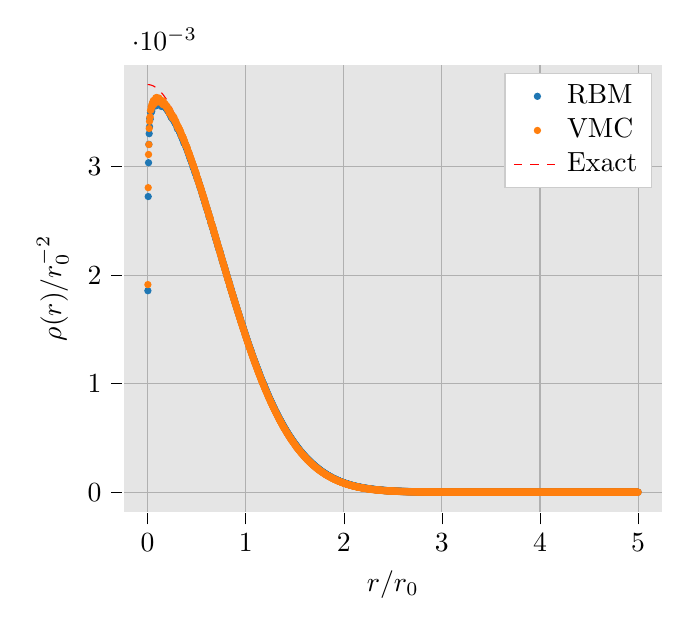
\begin{tikzpicture}

\definecolor{color0}{rgb}{0.12156862745098,0.466666666666667,0.705882352941177}
\definecolor{color1}{rgb}{1,0.498039215686275,0.0549019607843137}

\begin{axis}[
axis line style={white},
axis background/.style={fill=white!89.80392156862746!black},
legend cell align={left},
legend style={draw=white!80.0!black},
tick align=outside,
tick pos=left,
x grid style={white!69.01960784313725!black},
xlabel={\(\displaystyle r / r_0\)},
xmajorgrids,
xmin=-0.25, xmax=5.25,
xtick style={color=black},
y grid style={white!69.01960784313725!black},
ylabel={\(\displaystyle \rho(r) / r_0^{-2}\)},
ymajorgrids,
ymin=-0.000187835169142783, ymax=0.00394453855199845,
ytick style={color=black}
]
\addplot [semithick, color0, opacity=1.0, mark=*, mark size=1, mark options={solid}, only marks]
table {%
0 nan
0.00333555703802535 0.00185646877100309
0.0066711140760507 0.0027246950887207
0.0100066711140761 0.00303635342797842
0.0133422281521014 0.00320558165931794
0.0166777851901268 0.00330448810747907
0.0200133422281521 0.00336812406027423
0.0233488992661775 0.00344246673629199
0.0266844563042028 0.00343854448685171
0.0300200133422282 0.00349986779995693
0.0333555703802535 0.00350266269626468
0.0366911274182789 0.00349876179820948
0.0400266844563042 0.00352707693754115
0.0433622414943296 0.00351157854195228
0.0466977985323549 0.00356088578825543
0.0500333555703803 0.0035786509947023
0.0533689126084056 0.00358478332601282
0.056704469646431 0.00356404403489878
0.0600400266844563 0.0035628534370099
0.0633755837224817 0.00359084470329943
0.066711140760507 0.00358165961837476
0.0700466977985324 0.00358271259751591
0.0733822548365577 0.00359745003521503
0.0767178118745831 0.0036015276856059
0.0800533689126084 0.0035895784912467
0.0833889259506338 0.00355992190132711
0.0867244829886591 0.00360039554090835
0.0900600400266845 0.00361068939647317
0.0933955970647098 0.00359613906017076
0.0967311541027352 0.00357958754007763
0.100066711140761 0.00358508473639895
0.103402268178786 0.00358002351683597
0.106737825216811 0.003592027450634
0.110073382254837 0.00359210436010236
0.113408939292862 0.00359109360227858
0.116744496330887 0.00360030556945642
0.120080053368913 0.00357175874387281
0.123415610406938 0.00358601636850153
0.126751167444963 0.00358558372201427
0.130086724482989 0.00358304020440912
0.133422281521014 0.00357369416389768
0.136757838559039 0.00357338520154401
0.140093395597065 0.00355575006842943
0.14342895263509 0.00358437995862504
0.146764509673115 0.0035985485639777
0.150100066711141 0.00357069376050849
0.153435623749166 0.00357390753385877
0.156771180787191 0.00355999829749152
0.160106737825217 0.00357352838818531
0.163442294863242 0.00356465034246586
0.166777851901268 0.00355191863354705
0.170113408939293 0.00355218103788321
0.173448965977318 0.00356109626363995
0.176784523015344 0.0035524776128086
0.180120080053369 0.00355061434860344
0.183455637091394 0.00355427112915581
0.18679119412942 0.00353896699011087
0.190126751167445 0.00353624471660634
0.19346230820547 0.00353405283998878
0.196797865243496 0.00353552432354009
0.200133422281521 0.00352262702420412
0.203468979319546 0.00352759036834793
0.206804536357572 0.00351660535735208
0.210140093395597 0.00351058809317095
0.213475650433622 0.0035097578282518
0.216811207471648 0.00350474432491742
0.220146764509673 0.00349423316943276
0.223482321547698 0.00349246218357698
0.226817878585724 0.00349544818884054
0.230153435623749 0.00348199285357953
0.233488992661775 0.00348165165225705
0.2368245496998 0.00347096018976151
0.240160106737825 0.00345544173577109
0.243495663775851 0.0034625049234497
0.246831220813876 0.00345932625160739
0.250166777851901 0.00344450035608163
0.253502334889927 0.00346036717566946
0.256837891927952 0.00345990227735314
0.260173448965977 0.00344036559575812
0.263509006004003 0.00343728126863965
0.266844563042028 0.00342436449823154
0.270180120080053 0.00342424931278095
0.273515677118079 0.00342591732978846
0.276851234156104 0.00341143339842925
0.280186791194129 0.00340178807742633
0.283522348232155 0.00341340976192497
0.28685790527018 0.00339516433157446
0.290193462308205 0.00339596719901548
0.293529019346231 0.00338362552170301
0.296864576384256 0.00338042431333514
0.300200133422282 0.00336995078988713
0.303535690460307 0.00335001655280143
0.306871247498332 0.00336237462737517
0.310206804536358 0.0033641076121963
0.313542361574383 0.00334788700549024
0.316877918612408 0.00334391431657073
0.320213475650434 0.00333632526453758
0.323549032688459 0.00332661812695206
0.326884589726484 0.00332058845492486
0.33022014676451 0.00331426874995922
0.333555703802535 0.00331007461198125
0.33689126084056 0.00330580074835418
0.340226817878586 0.00329067287378072
0.343562374916611 0.00328202231276048
0.346897931954636 0.00327723723614908
0.350233488992662 0.00327718110937987
0.353569046030687 0.00327088172832386
0.356904603068712 0.00325341295236912
0.360240160106738 0.00325199276968315
0.363575717144763 0.00324346132789468
0.366911274182789 0.00324124274268841
0.370246831220814 0.00321805871628479
0.373582388258839 0.00323504550316723
0.376917945296865 0.00322236558633832
0.38025350233489 0.00321839376396087
0.383589059372915 0.00320821214996052
0.386924616410941 0.00319508804255195
0.390260173448966 0.00319228025738274
0.393595730486991 0.00317687197172204
0.396931287525017 0.0031765219218305
0.400266844563042 0.00316139489671138
0.403602401601067 0.00316689877264731
0.406937958639093 0.00314495100614627
0.410273515677118 0.00313922592890107
0.413609072715143 0.00313733739805028
0.416944629753169 0.00312625132251892
0.420280186791194 0.00311431824785721
0.423615743829219 0.00310609681390332
0.426951300867245 0.00309323607556527
0.43028685790527 0.00309678079393164
0.433622414943296 0.00307777269522143
0.436957971981321 0.00306854263487795
0.440293529019346 0.00306754815744534
0.443629086057372 0.00305424933486888
0.446964643095397 0.00305599704218
0.450300200133422 0.0030356324786912
0.453635757171448 0.00303326759811615
0.456971314209473 0.00302461542350519
0.460306871247498 0.00302171179301586
0.463642428285524 0.00299578347172796
0.466977985323549 0.00299921497110257
0.470313542361574 0.00299369423886071
0.4736490993996 0.00297451297029265
0.476984656437625 0.00297753145700958
0.48032021347565 0.00296564757489892
0.483655770513676 0.00294503156117008
0.486991327551701 0.00294543334159014
0.490326884589726 0.00293695174969122
0.493662441627752 0.00292701403328729
0.496997998665777 0.00291938339468991
0.500333555703803 0.00290488369773765
0.503669112741828 0.00290328863615181
0.507004669779853 0.00288927381247706
0.510340226817879 0.00288536885273767
0.513675783855904 0.00287536113757937
0.517011340893929 0.00286818304986506
0.520346897931955 0.00285604467636001
0.52368245496998 0.00284680661114199
0.527018012008005 0.00284558944189233
0.530353569046031 0.00282815174801459
0.533689126084056 0.00281359539708594
0.537024683122081 0.00281699406298746
0.540360240160107 0.00280041100147604
0.543695797198132 0.00279358307967077
0.547031354236157 0.00278504800741204
0.550366911274183 0.00276867709154429
0.553702468312208 0.00276680076612235
0.557038025350234 0.00275419064640874
0.560373582388259 0.00274108281055876
0.563709139426284 0.00273232876478296
0.56704469646431 0.00272512641181871
0.570380253502335 0.00271113402493648
0.57371581054036 0.00270256914490002
0.577051367578386 0.00269620919384663
0.580386924616411 0.00268776050566805
0.583722481654436 0.00267218767711191
0.587058038692462 0.00266104767734888
0.590393595730487 0.00266093820023286
0.593729152768512 0.00264590413550574
0.597064709806538 0.00263357301918812
0.600400266844563 0.00261781131234002
0.603735823882588 0.00262034472390997
0.607071380920614 0.00261119917343381
0.610406937958639 0.00259755740283735
0.613742494996664 0.00258804896271814
0.61707805203469 0.00257844958446506
0.620413609072715 0.00256939360824292
0.62374916611074 0.00256257967360067
0.627084723148766 0.00253677066845897
0.630420280186791 0.00253737440537222
0.633755837224817 0.00252891736147455
0.637091394262842 0.00252119788804455
0.640426951300867 0.00251025529946178
0.643762508338893 0.00249163004004797
0.647098065376918 0.00248212215684192
0.650433622414943 0.00247518209089401
0.653769179452969 0.00247038468884836
0.657104736490994 0.0024563174449088
0.660440293529019 0.00244537152427468
0.663775850567045 0.00243865649459079
0.66711140760507 0.0024266851597658
0.670446964643095 0.00241801963161305
0.673782521681121 0.0024120931803154
0.677118078719146 0.00239107550010192
0.680453635757171 0.00238766025149924
0.683789192795197 0.00237879920286154
0.687124749833222 0.00236152776289358
0.690460306871247 0.00235812366883852
0.693795863909273 0.00234346680603796
0.697131420947298 0.00233158698398009
0.700466977985324 0.00232815019011952
0.703802535023349 0.00231685761727141
0.707138092061374 0.00230443078065648
0.7104736490994 0.00229250810046006
0.713809206137425 0.00228299238048745
0.71714476317545 0.00227416927407495
0.720480320213476 0.00226297091176283
0.723815877251501 0.00225537297928947
0.727151434289526 0.00223941933935631
0.730486991327552 0.00223334811383871
0.733822548365577 0.00222843061004304
0.737158105403602 0.00221780861768277
0.740493662441628 0.00220883750767187
0.743829219479653 0.00219475959927507
0.747164776517678 0.00218344962039334
0.750500333555704 0.00217546690984546
0.753835890593729 0.0021615009314906
0.757171447631754 0.00215336946869597
0.76050700466978 0.00213785916201161
0.763842561707805 0.00212924433286668
0.767178118745831 0.00212376236065153
0.770513675783856 0.00211086198374758
0.773849232821881 0.00210324876086151
0.777184789859907 0.00208757092154531
0.780520346897932 0.0020888287777646
0.783855903935957 0.00207051235426894
0.787191460973983 0.00206322422089545
0.790527018012008 0.00205019136536729
0.793862575050033 0.00204666816531213
0.797198132088059 0.00203051314821576
0.800533689126084 0.00202121420787254
0.803869246164109 0.0020128560785367
0.807204803202135 0.00199835493621093
0.81054036024016 0.00199365345866616
0.813875917278185 0.00198526443860805
0.817211474316211 0.0019680270739028
0.820547031354236 0.00196397804633586
0.823882588392261 0.00195042095095802
0.827218145430287 0.00194289179094033
0.830553702468312 0.0019332640437538
0.833889259506338 0.00192243358484715
0.837224816544363 0.00191388499330079
0.840560373582388 0.00189306990841137
0.843895930620414 0.00188970990695435
0.847231487658439 0.00188070889761843
0.850567044696464 0.00187190743005389
0.85390260173449 0.00186475969732041
0.857238158772515 0.00184981066141943
0.86057371581054 0.00183695037749962
0.863909272848566 0.00182977284569795
0.867244829886591 0.00181783343969015
0.870580386924616 0.00181484705172643
0.873915943962642 0.00179932336980109
0.877251501000667 0.00179059773465053
0.880587058038692 0.0017856236297906
0.883922615076718 0.00177047282054766
0.887258172114743 0.00176283789049441
0.890593729152768 0.00174772704640566
0.893929286190794 0.00174459194276867
0.897264843228819 0.00173241400110294
0.900600400266845 0.00172300546984476
0.90393595730487 0.00171508232561612
0.907271514342895 0.00170455189206798
0.910607071380921 0.00169217752736684
0.913942628418946 0.00168554568126141
0.917278185456971 0.00167169473852509
0.920613742494997 0.00166653614796182
0.923949299533022 0.00165382127978502
0.927284856571047 0.00164776110156619
0.930620413609073 0.00163623235619509
0.933955970647098 0.00162780515161328
0.937291527685123 0.00161899795183206
0.940627084723149 0.00160796552711987
0.943962641761174 0.0016010567275017
0.947298198799199 0.00159053334531345
0.950633755837225 0.0015763411308754
0.95396931287525 0.00156894855581497
0.957304869913275 0.00155986949421105
0.960640426951301 0.00155498074886521
0.963975983989326 0.00154955582017751
0.967311541027352 0.00153574506557396
0.970647098065377 0.00152355012389076
0.973982655103402 0.00151971980003825
0.977318212141428 0.00150790407195547
0.980653769179453 0.00149842902126978
0.983989326217478 0.00148486626853637
0.987324883255504 0.00147947991569335
0.990660440293529 0.00147168976666735
0.993995997331554 0.00146106100895882
0.99733155436958 0.00145171192070661
1.00066711140761 0.00144340063332271
1.00400266844563 0.00143406855994014
1.00733822548366 0.00142127826508681
1.01067378252168 0.00141598421437808
1.01400933955971 0.00140728761660899
1.01734489659773 0.00139639272340548
1.02068045363576 0.00138633196690438
1.02401601067378 0.00138072375998635
1.02735156771181 0.00137002336729873
1.03068712474983 0.00136140234479996
1.03402268178786 0.00135372261102964
1.03735823882588 0.00134382018889493
1.04069379586391 0.00133524906443537
1.04402935290193 0.00132690814362145
1.04736490993996 0.00132093145353253
1.05070046697799 0.00131092275710472
1.05403602401601 0.00130297212622464
1.05737158105404 0.00129560999484676
1.06070713809206 0.00128216462666574
1.06404269513009 0.00127326157741892
1.06737825216811 0.0012672450322769
1.07071380920614 0.00125834149879285
1.07404936624416 0.00125033367584242
1.07738492328219 0.00124095024850638
1.08072048032021 0.00123205909926926
1.08405603735824 0.00122423236851256
1.08739159439626 0.00121804122823267
1.09072715143429 0.00121026803054425
1.09406270847231 0.00120062650341416
1.09739826551034 0.00119062882537882
1.10073382254837 0.00118742738961335
1.10406937958639 0.00117788860994695
1.10740493662442 0.0011676318130748
1.11074049366244 0.00115960203374362
1.11407605070047 0.00115326340910995
1.11741160773849 0.001142375954335
1.12074716477652 0.0011378124643764
1.12408272181454 0.00112967864683625
1.12741827885257 0.00112153653514794
1.13075383589059 0.00111075571206842
1.13408939292862 0.00110701974381173
1.13742494996664 0.00109689242006688
1.14076050700467 0.00108894044247854
1.1440960640427 0.0010829894860497
1.14743162108072 0.00107259307382909
1.15076717811875 0.00106209967307207
1.15410273515677 0.00105679866533603
1.1574382921948 0.00105066401518563
1.16077384923282 0.00103947654976659
1.16410940627085 0.00103595354260701
1.16744496330887 0.0010261478234451
1.1707805203469 0.00101879989257171
1.17411607738492 0.0010127127419478
1.17745163442295 0.00100488282158732
1.18078719146097 0.00100019483802727
1.184122748499 0.000994506077570849
1.18745830553702 0.000986348093626786
1.19079386257505 0.00097761595265914
1.19412941961308 0.000971934146075379
1.1974649766511 0.000959313925534543
1.20080053368913 0.000954721964888666
1.20413609072715 0.000949233679741417
1.20747164776518 0.000940751924018615
1.2108072048032 0.000934648470983682
1.21414276184123 0.000928233482173713
1.21747831887925 0.000915571996298752
1.22081387591728 0.000910930464645398
1.2241494329553 0.000906292724794165
1.22748498999333 0.000900433744926362
1.23082054703135 0.000892114148984907
1.23415610406938 0.000883212116266898
1.2374916611074 0.000877967021021964
1.24082721814543 0.000869701549196939
1.24416277518346 0.000864511102297652
1.24749833222148 0.000858085916958405
1.25083388925951 0.000851448609984111
1.25416944629753 0.000844941053641796
1.25750500333556 0.000838943357479083
1.26084056037358 0.000829396135245964
1.26417611741161 0.000826604789573614
1.26751167444963 0.000818749730726738
1.27084723148766 0.00081208890299536
1.27418278852568 0.000806898700799169
1.27751834556371 0.000796286605367556
1.28085390260173 0.000793004731949709
1.28418945963976 0.000786499621024305
1.28752501667779 0.000778148198222809
1.29086057371581 0.000775430577486242
1.29419613075384 0.000769600715110272
1.29753168779186 0.000760618372184396
1.30086724482989 0.000752522669212837
1.30420280186791 0.00074790533788571
1.30753835890594 0.000741104669958008
1.31087391594396 0.000737102968878251
1.31420947298199 0.000734402609915765
1.31754503002001 0.000724695177429183
1.32088058705804 0.000719854356567617
1.32421614409606 0.000712337031659553
1.32755170113409 0.000706585807135539
1.33088725817211 0.000702939289854961
1.33422281521014 0.000694687095828121
1.33755837224817 0.000688835137675077
1.34089392928619 0.000685676319868222
1.34422948632422 0.000677085354128483
1.34756504336224 0.00066990587994588
1.35090060040027 0.000664448946239267
1.35423615743829 0.000662620430890681
1.35757171447632 0.000657130655485683
1.36090727151434 0.000649989079957517
1.36424282855237 0.000644358459816953
1.36757838559039 0.000639369621918604
1.37091394262842 0.000632789804944526
1.37424949966644 0.000628217191068741
1.37758505670447 0.000621783817947286
1.38092061374249 0.000617939739611369
1.38425617078052 0.00061166434446416
1.38759172781855 0.000606648209915379
1.39092728485657 0.000600583751289521
1.3942628418946 0.000595370337537918
1.39759839893262 0.000590344252599872
1.40093395597065 0.000585032079288179
1.40426951300867 0.000581224402428398
1.4076050700467 0.000576363407498772
1.41094062708472 0.000571144503439125
1.41427618412275 0.000566207682327088
1.41761174116077 0.00055789534466944
1.4209472981988 0.000556717718830979
1.42428285523682 0.000551127832218782
1.42761841227485 0.000546749477512923
1.43095396931288 0.000539828492552546
1.4342895263509 0.000536879316763667
1.43762508338893 0.00053142777110048
1.44096064042695 0.00052601440340938
1.44429619746498 0.000521260121621748
1.447631754503 0.000517844509547657
1.45096731154103 0.000513092317598165
1.45430286857905 0.000509682449096596
1.45763842561708 0.000503282986278535
1.4609739826551 0.000498718204225458
1.46430953969313 0.000495702179980957
1.46764509673115 0.000488779537121945
1.47098065376918 0.000486815985799944
1.4743162108072 0.000481067342437213
1.47765176784523 0.000476250924629899
1.48098732488326 0.000468824971189652
1.48432288192128 0.000468877568021795
1.48765843895931 0.00046334087362335
1.49099399599733 0.000460314530173357
1.49432955303536 0.000455518189299738
1.49766511007338 0.000449721627659853
1.50100066711141 0.000446762530736329
1.50433622414943 0.000442884073507625
1.50767178118746 0.00043893621000934
1.51100733822548 0.000434605831464672
1.51434289526351 0.000430243831695261
1.51767845230153 0.000426898279476145
1.52101400933956 0.000421745959020281
1.52434956637759 0.000419250994653156
1.52768512341561 0.000413841366001465
1.53102068045364 0.000410207536415729
1.53435623749166 0.000405804647739725
1.53769179452969 0.000402263216674271
1.54102735156771 0.000398611143307223
1.54436290860574 0.000393288888619543
1.54769846564376 0.000391191941929934
1.55103402268179 0.000386203403447624
1.55436957971981 0.000382473903914566
1.55770513675784 0.000378625190727641
1.56104069379586 0.000374334837453117
1.56437625083389 0.000372356747247602
1.56771180787191 0.000369530066192651
1.57104736490994 0.000366202274807176
1.57438292194797 0.000361424955832214
1.57771847898599 0.00035786838063192
1.58105403602402 0.000353471486402327
1.58438959306204 0.000350656170640793
1.58772515010007 0.000346862796045584
1.59106070713809 0.000343979390097375
1.59439626417612 0.000338333101106015
1.59773182121414 0.000337417400569784
1.60106737825217 0.000334525112210864
1.60440293529019 0.000330039074915955
1.60773849232822 0.00032707381484918
1.61107404936624 0.000324738290593454
1.61440960640427 0.000319035307506067
1.61774516344229 0.0003169537835861
1.62108072048032 0.000313510101831988
1.62441627751835 0.00031176918085949
1.62775183455637 0.000305989263582393
1.6310873915944 0.000306185210784994
1.63442294863242 0.000301997101856832
1.63775850567045 0.000297981417463275
1.64109406270847 0.000295113515490498
1.6444296197465 0.000293725227193149
1.64776517678452 0.000289523701229156
1.65110073382255 0.00028622528105623
1.65443629086057 0.000283924606177408
1.6577718478986 0.000282250455083191
1.66110740493662 0.000278403496962454
1.66444296197465 0.000274514629684408
1.66777851901268 0.000273046243945456
1.6711140760507 0.000268978825474821
1.67444963308873 0.000266707909061474
1.67778519012675 0.000263221641179204
1.68112074716478 0.00026062669031092
1.6844563042028 0.000258626063531817
1.68779186124083 0.000256758110723031
1.69112741827885 0.000252625680232777
1.69446297531688 0.000250626080276257
1.6977985323549 0.000247841701729574
1.70113408939293 0.000245106926000366
1.70446964643095 0.000241355881520206
1.70780520346898 0.000238924459524765
1.711140760507 0.00023728576713877
1.71447631754503 0.000234638869723357
1.71781187458306 0.000231748779485989
1.72114743162108 0.000229530699965713
1.72448298865911 0.000228435470754463
1.72781854569713 0.000225851489051906
1.73115410273516 0.000223107040519962
1.73448965977318 0.000220583080947117
1.73782521681121 0.00021732346252213
1.74116077384923 0.000215453309240698
1.74449633088726 0.000214003993744955
1.74783188792528 0.000210554711873792
1.75116744496331 0.00020839811592947
1.75450300200133 0.000205807762535244
1.75783855903936 0.00020388798201692
1.76117411607738 0.000201489106635063
1.76450967311541 0.000199028441572879
1.76784523015344 0.000197310373345725
1.77118078719146 0.000194988215033365
1.77451634422949 0.000193179746896755
1.77785190126751 0.000190790152565915
1.78118745830554 0.000188748171381777
1.78452301534356 0.00018609307714856
1.78785857238159 0.000184120848993385
1.79119412941961 0.000182807465739092
1.79452968645764 0.000180937296525583
1.79786524349566 0.000178453046429252
1.80120080053369 0.000176287323473654
1.80453635757171 0.000174430460138059
1.80787191460974 0.000172925639927233
1.81120747164777 0.000171260442802803
1.81454302868579 0.000168131387661652
1.81787858572382 0.000166340523760249
1.82121414276184 0.000164421322843846
1.82454969979987 0.000163285181944408
1.82788525683789 0.000161049149501182
1.83122081387592 0.000159311185788541
1.83455637091394 0.000157108444983411
1.83789192795197 0.000155524775473853
1.84122748498999 0.000153679386855065
1.84456304202802 0.000151779428996157
1.84789859906604 0.000150346903462246
1.85123415610407 0.000148123283555568
1.85456971314209 0.000146640982514742
1.85790527018012 0.000145649841845437
1.86124082721815 0.00014317376365094
1.86457638425617 0.000142549417217249
1.8679119412942 0.000140014323245479
1.87124749833222 0.00013800639398663
1.87458305537025 0.000136932366873242
1.87791861240827 0.000135128023973018
1.8812541694463 0.000133134774849642
1.88458972648432 0.00013199941716552
1.88792528352235 0.000130579344789168
1.89126084056037 0.000129169500713919
1.8945963975984 0.000127104682644978
1.89793195463642 0.000126239857936184
1.90126751167445 0.000124401440362796
1.90460306871247 0.000123409629735271
1.9079386257505 0.000120711697997387
1.91127418278853 0.000121025523229355
1.91460973982655 0.000118754164556183
1.91794529686458 0.000117567491887088
1.9212808539026 0.00011604299865979
1.92461641094063 0.000114520370455841
1.92795196797865 0.000113183345103311
1.93128752501668 0.000112572165070669
1.9346230820547 0.000110266879623784
1.93795863909273 0.000108635641520589
1.94129419613075 0.00010744390441034
1.94462975316878 0.000106578862935023
1.9479653102068 0.00010512278401015
1.95130086724483 0.000103775104132507
1.95463642428286 0.000102592501729656
1.95797198132088 0.000101138332087088
1.96130753835891 0.000100119694865666
1.96464309539693 9.90916766830314e-05
1.96797865243496 9.7510950582944e-05
1.97131420947298 9.69909969800185e-05
1.97464976651101 9.53141843773503e-05
1.97798532354903 9.45485058853442e-05
1.98132088058706 9.32346187793864e-05
1.98465643762508 9.22368280843766e-05
1.98799199466311 9.07088948138094e-05
1.99132755170113 8.95226023964556e-05
1.99466310873916 8.88873799766034e-05
1.99799866577718 8.7330422958932e-05
2.00133422281521 8.63743523247545e-05
2.00466977985324 8.4983230551941e-05
2.00800533689126 8.38195793211828e-05
2.01134089392929 8.27830237174802e-05
2.01467645096731 8.22572715426987e-05
2.01801200800534 8.11452014256696e-05
2.02134756504336 8.02136868101575e-05
2.02468312208139 7.91362741936441e-05
2.02801867911941 7.79277444784179e-05
2.03135423615744 7.65730858791206e-05
2.03468979319546 7.61381501586543e-05
2.03802535023349 7.50136499918808e-05
2.04136090727151 7.46659611072449e-05
2.04469646430954 7.3414504952649e-05
2.04803202134757 7.20037905839827e-05
2.05136757838559 7.14327912180833e-05
2.05470313542362 7.07467469128837e-05
2.05803869246164 6.99755276164968e-05
2.06137424949967 6.82469730429098e-05
2.06470980653769 6.83831951498999e-05
2.06804536357572 6.6705212105409e-05
2.07138092061374 6.58994031572587e-05
2.07471647765177 6.53356571520869e-05
2.07805203468979 6.46111625149261e-05
2.08138759172782 6.31175480086653e-05
2.08472314876584 6.25346540461302e-05
2.08805870580387 6.19594001995034e-05
2.09139426284189 6.16072865268631e-05
2.09472981987992 5.98169592878019e-05
2.09806537691795 6.00637409265036e-05
2.10140093395597 5.8333739613015e-05
2.104736490994 5.82762065219193e-05
2.10807204803202 5.71653065356943e-05
2.11140760507005 5.62459571048396e-05
2.11474316210807 5.61121202864754e-05
2.1180787191461 5.4970005046328e-05
2.12141427618412 5.41308237538807e-05
2.12474983322215 5.32586603276699e-05
2.12808539026017 5.2949962503722e-05
2.1314209472982 5.17103414817038e-05
2.13475650433622 5.12565487203036e-05
2.13809206137425 5.12063373450126e-05
2.14142761841227 4.98886686180103e-05
2.1447631754503 4.96806817473254e-05
2.14809873248833 4.83694741896581e-05
2.15143428952635 4.84326344940424e-05
2.15476984656438 4.75330880704864e-05
2.1581054036024 4.67201768283067e-05
2.16144096064043 4.68043646568732e-05
2.16477651767845 4.57128812034579e-05
2.16811207471648 4.48711117266181e-05
2.1714476317545 4.39824298512868e-05
2.17478318879253 4.36633205204855e-05
2.17811874583055 4.34982645787804e-05
2.18145430286858 4.22527587161107e-05
2.1847898599066 4.18975915115717e-05
2.18812541694463 4.14307288574693e-05
2.19146097398266 4.10828987573e-05
2.19479653102068 4.0063012119525e-05
2.19813208805871 3.95701234637144e-05
2.20146764509673 3.92042745541963e-05
2.20480320213476 3.87788442763266e-05
2.20813875917278 3.78758864125422e-05
2.21147431621081 3.73788554375665e-05
2.21480987324883 3.71943057538448e-05
2.21814543028686 3.6504980009638e-05
2.22148098732488 3.58157494698864e-05
2.22481654436291 3.58123356861129e-05
2.22815210140093 3.48564621768794e-05
2.23148765843896 3.45065128071446e-05
2.23482321547698 3.38916144190583e-05
2.23815877251501 3.34480998119972e-05
2.24149432955304 3.3255938804652e-05
2.24482988659106 3.25962934994842e-05
2.24816544362909 3.26630637968977e-05
2.25150100066711 3.16087549659145e-05
2.25483655770514 3.14486635532944e-05
2.25817211474316 3.10835987139368e-05
2.26150767178119 3.01230946317791e-05
2.26484322881921 2.99905957264027e-05
2.26817878585724 2.97085872407479e-05
2.27151434289526 2.89691955898873e-05
2.27484989993329 2.90125375564674e-05
2.27818545697131 2.81203493638226e-05
2.28152101400934 2.79071405836773e-05
2.28485657104736 2.76854339966475e-05
2.28819212808539 2.70770858036019e-05
2.29152768512342 2.67485863431672e-05
2.29486324216144 2.64549743876362e-05
2.29819879919947 2.62676825016444e-05
2.30153435623749 2.56396591546279e-05
2.30486991327552 2.54978673285415e-05
2.30820547031354 2.50091427007011e-05
2.31154102735157 2.47016546434927e-05
2.31487658438959 2.42979254528524e-05
2.31821214142762 2.40543229749743e-05
2.32154769846564 2.36073307129817e-05
2.32488325550367 2.31252961440868e-05
2.32821881254169 2.28288336372178e-05
2.33155436957972 2.2299429347578e-05
2.33488992661775 2.21553074371569e-05
2.33822548365577 2.21907777835179e-05
2.3415610406938 2.13324547410628e-05
2.34489659773182 2.11786302091335e-05
2.34823215476985 2.1008895524509e-05
2.35156771180787 2.09814276679517e-05
2.3549032688459 2.07509756693155e-05
2.35823882588392 1.99263386813078e-05
2.36157438292195 2.00783901749292e-05
2.36490993995997 1.9679056670792e-05
2.368245496998 1.9169700557825e-05
2.37158105403602 1.91371893953472e-05
2.37491661107405 1.85893855048984e-05
2.37825216811207 1.82248176199588e-05
2.3815877251501 1.82481077927799e-05
2.38492328218813 1.77466143177072e-05
2.38825883922615 1.76198786617723e-05
2.39159439626418 1.72320983936028e-05
2.3949299533022 1.7060178953369e-05
2.39826551034023 1.7055658643105e-05
2.40160106737825 1.63633871899997e-05
2.40493662441628 1.63817361949082e-05
2.4082721814543 1.57597175703932e-05
2.41160773849233 1.58557098483783e-05
2.41494329553035 1.56866620847416e-05
2.41827885256838 1.53017454810542e-05
2.4216144096064 1.50759542044881e-05
2.42494996664443 1.4514736193566e-05
2.42828552368245 1.4458665255902e-05
2.43162108072048 1.44347722967404e-05
2.43495663775851 1.42758168537725e-05
2.43829219479653 1.38591051964143e-05
2.44162775183456 1.37907604538843e-05
2.44496330887258 1.35539349873211e-05
2.44829886591061 1.33836066821893e-05
2.45163442294863 1.32642938014612e-05
2.45496997998666 1.30108320285242e-05
2.45830553702468 1.24051547349094e-05
2.46164109406271 1.24801276066053e-05
2.46497665110073 1.22180773080742e-05
2.46831220813876 1.23717484732169e-05
2.47164776517678 1.21367323828092e-05
2.47498332221481 1.21270227299413e-05
2.47831887925284 1.18265867988548e-05
2.48165443629086 1.15194453291214e-05
2.48498999332889 1.10974927377704e-05
2.48832555036691 1.11835521237036e-05
2.49166110740494 1.10365280926185e-05
2.49499666444296 1.0666586805194e-05
2.49833222148099 1.05158165641585e-05
2.50166777851901 1.03163458851042e-05
2.50500333555704 1.02636420844599e-05
2.50833889259506 1.00103811122506e-05
2.51167444963309 1.00652073890343e-05
2.51501000667111 9.84558806989401e-06
2.51834556370914 9.70276507054816e-06
2.52168112074716 9.45637029613818e-06
2.52501667778519 9.45908103096667e-06
2.52835223482322 9.00110172058067e-06
2.53168779186124 9.11097640055452e-06
2.53502334889927 8.89564442469621e-06
2.53835890593729 8.8247603291917e-06
2.54169446297532 8.70918514423499e-06
2.54503002001334 8.47669576337014e-06
2.54836557705137 8.39286616835975e-06
2.55170113408939 8.38533365133259e-06
2.55503669112742 8.26320901921123e-06
2.55837224816544 7.92362427426094e-06
2.56170780520347 7.80541583739162e-06
2.56504336224149 7.56992950850013e-06
2.56837891927952 7.73090951190358e-06
2.57171447631755 7.59294024003747e-06
2.57505003335557 7.44042115208642e-06
2.5783855903936 7.16749148245905e-06
2.58172114743162 7.24192086306777e-06
2.58505670446965 7.09638491739459e-06
2.58839226150767 7.07156223164801e-06
2.5917278185457 6.72984116618412e-06
2.59506337558372 6.57369078642978e-06
2.59839893262175 6.64418376201893e-06
2.60173448965977 6.41603647117246e-06
2.6050700466978 6.55012378638113e-06
2.60840560373582 6.24741527613508e-06
2.61174116077385 6.10463640983905e-06
2.61507671781187 5.93160541423056e-06
2.6184122748499 5.99902658966185e-06
2.62174783188793 5.875515438149e-06
2.62508338892595 5.69925712444049e-06
2.62841894596398 5.51134524226503e-06
2.631754503002 5.64105217649019e-06
2.63509006004003 5.33923005744575e-06
2.63842561707805 5.39026108760686e-06
2.64176117411608 5.21780403977044e-06
2.6450967311541 5.21868777231274e-06
2.64843228819213 5.14751238780054e-06
2.65176784523015 4.95243631356779e-06
2.65510340226818 5.06394233470907e-06
2.6584389593062 4.89957761469855e-06
2.66177451634423 4.89343779312625e-06
2.66511007338225 4.67825682491954e-06
2.66844563042028 4.75995502058686e-06
2.67178118745831 4.53234194518742e-06
2.67511674449633 4.61934820292781e-06
2.67845230153436 4.44202404899478e-06
2.68178785857238 4.21442880469835e-06
2.68512341561041 4.47346793751104e-06
2.68845897264843 4.1741904861835e-06
2.69179452968646 4.26232382466895e-06
2.69513008672448 4.108920794889e-06
2.69846564376251 3.98272215801494e-06
2.70180120080053 4.0281417664125e-06
2.70513675783856 3.87397319511134e-06
2.70847231487658 3.88297025426881e-06
2.71180787191461 3.72127066457687e-06
2.71514342895264 3.67872823740865e-06
2.71847898599066 3.70528007077976e-06
2.72181454302869 3.51417109282598e-06
2.72515010006671 3.4104617052096e-06
2.72848565710474 3.44568548108544e-06
2.73182121414276 3.33388191331056e-06
2.73515677118079 3.28249945124787e-06
2.73849232821881 3.33697442661436e-06
2.74182788525684 3.23531148376108e-06
2.74516344229486 3.2429666685674e-06
2.74849899933289 3.02873543343544e-06
2.75183455637091 2.95451926264685e-06
2.75517011340894 2.94417505940455e-06
2.75850567044696 2.96924185592673e-06
2.76184122748499 2.83659339673486e-06
2.76517678452302 2.79787107852561e-06
2.76851234156104 2.79053856722229e-06
2.77184789859907 2.82397889833277e-06
2.77518345563709 2.78738739515313e-06
2.77851901267512 2.75325213565693e-06
2.78185456971314 2.57568875419604e-06
2.78519012675117 2.48636495767519e-06
2.78852568378919 2.482997521924e-06
2.79186124082722 2.45921018855597e-06
2.79519679786524 2.45627557019254e-06
2.79853235490327 2.45491558181482e-06
2.80186791194129 2.41206597315441e-06
2.80520346897932 2.25124332936891e-06
2.80853902601734 2.22045276035155e-06
2.81187458305537 2.30128926323262e-06
2.8152101400934 2.2428516927357e-06
2.81854569713142 2.13357695166918e-06
2.82188125416945 2.20956549986487e-06
2.82521681120747 1.96355101389991e-06
2.8285523682455 2.05933605583127e-06
2.83188792528352 2.09602699612194e-06
2.83522348232155 1.96822593962695e-06
2.83855903935957 1.91838807879341e-06
2.8418945963976 1.8987696539773e-06
2.84523015343562 1.76856551409315e-06
2.84856571047365 1.76803469419526e-06
2.85190126751167 1.85595728671147e-06
2.8552368245497 1.76467202278434e-06
2.85857238158773 1.70237558067993e-06
2.86190793862575 1.62297900223482e-06
2.86524349566378 1.63716654224801e-06
2.8685790527018 1.54235454246811e-06
2.87191460973983 1.50772024635866e-06
2.87525016677785 1.51970341068031e-06
2.87858572381588 1.52899173648412e-06
2.8819212808539 1.5386391302031e-06
2.88525683789193 1.48782375362292e-06
2.88859239492995 1.43940387211791e-06
2.89192795196798 1.45746475482226e-06
2.895263509006 1.48987898866355e-06
2.89859906604403 1.3799481262228e-06
2.90193462308205 1.36173244040621e-06
2.90527018012008 1.31147021991016e-06
2.90860573715811 1.28243960370204e-06
2.91194129419613 1.22146064631977e-06
2.91527685123416 1.25392238440071e-06
2.91861240827218 1.20739520494568e-06
2.92194796531021 1.27132873950189e-06
2.92528352234823 1.17652218307099e-06
2.92861907938626 1.1942816997719e-06
2.93195463642428 1.11885630147416e-06
2.93529019346231 1.134772738853e-06
2.93862575050033 1.15251916916812e-06
2.94196130753836 1.14934844828288e-06
2.94529686457638 1.09591364115548e-06
2.94863242161441 1.08649083243573e-06
2.95196797865243 1.07263085948272e-06
2.95530353569046 9.92000774213441e-07
2.95863909272849 9.83097686602399e-07
2.96197464976651 1.02827597331834e-06
2.96531020680454 9.74598262543125e-07
2.96864576384256 9.65005836857766e-07
2.97198132088059 9.40304455289277e-07
2.97531687791861 9.15289835416769e-07
2.97865243495664 9.17210553005981e-07
2.98198799199466 8.92645524265856e-07
2.98532354903269 8.73646193863523e-07
2.98865910607071 8.88451150347922e-07
2.99199466310874 8.21845041899598e-07
2.99533022014676 8.07748100993669e-07
2.99866577718479 8.18187926509816e-07
3.00200133422282 8.37372854555649e-07
3.00533689126084 7.84986871836354e-07
3.00867244829887 7.6625434183895e-07
3.01200800533689 7.1588380444609e-07
3.01534356237492 7.61649254088662e-07
3.01867911941294 6.87052183028289e-07
3.02201467645097 7.07706505661868e-07
3.02535023348899 6.44209188515757e-07
3.02868579052702 6.94921743270532e-07
3.03202134756504 6.42791786560826e-07
3.03535690460307 6.67017270083595e-07
3.03869246164109 6.59788267651217e-07
3.04202801867912 6.57983199385187e-07
3.04536357571714 5.78391014784858e-07
3.04869913275517 6.10855184779302e-07
3.0520346897932 5.77126772129591e-07
3.05537024683122 5.79368435743623e-07
3.05870580386925 5.72640888250457e-07
3.06204136090727 5.76315283757673e-07
3.0653769179453 5.2166150120869e-07
3.06871247498332 5.31101779195465e-07
3.07204803202135 5.24812872502347e-07
3.07538358905937 5.32802741325825e-07
3.0787191460974 5.37569119671998e-07
3.08205470313542 4.70086328307954e-07
3.08539026017345 5.16144920679837e-07
3.08872581721147 4.79013482295454e-07
3.0920613742495 4.67500898991996e-07
3.09539693128752 4.38296999579123e-07
3.09873248832555 4.11279618767716e-07
3.10206804536358 4.67053513286612e-07
3.1054036024016 4.39710103385617e-07
3.10873915943963 4.26890246449257e-07
3.11207471647765 4.14450294169056e-07
3.11541027351568 3.8936330978279e-07
3.1187458305537 3.970352854915e-07
3.12208138759173 3.80802865459426e-07
3.12541694462975 4.35841699318079e-07
3.12875250166778 3.86300731360165e-07
3.1320880587058 3.85889335480122e-07
3.13542361574383 3.4000490752538e-07
3.13875917278185 3.58163245038227e-07
3.14209472981988 3.42424538266204e-07
3.14543028685791 3.83903790758761e-07
3.14876584389593 3.42047379636744e-07
3.15210140093396 3.21504411871279e-07
3.15543695797198 3.28116168948009e-07
3.15877251501001 3.14922784163537e-07
3.16210807204803 3.51009563593643e-07
3.16544362908606 3.00053331991181e-07
3.16877918612408 3.31926385031221e-07
3.17211474316211 2.94236006419334e-07
3.17545030020013 2.73894311918129e-07
3.17878585723816 2.68086467639971e-07
3.18212141427618 2.89174744382507e-07
3.18545697131421 2.81985842444455e-07
3.18879252835223 2.58646569459017e-07
3.19212808539026 2.41884197019144e-07
3.19546364242829 2.80416343292075e-07
3.19879919946631 2.41722615096604e-07
3.20213475650434 2.86339866822858e-07
3.20547031354236 2.3061273323375e-07
3.20880587058039 2.35500006852887e-07
3.21214142761841 2.50620473994816e-07
3.21547698465644 2.17615797454367e-07
3.21881254169446 2.00012695232686e-07
3.22214809873249 2.14442171949717e-07
3.22548365577051 2.06399666500517e-07
3.22881921280854 2.04148356946345e-07
3.23215476984656 2.03937677527412e-07
3.23549032688459 1.88473298618074e-07
3.23882588392261 2.10628885129601e-07
3.24216144096064 1.92483175878322e-07
3.24549699799867 1.54098629627176e-07
3.24883255503669 1.83985805981499e-07
3.25216811207472 1.68958437427459e-07
3.25550366911274 1.93715691532445e-07
3.25883922615077 1.56833244555241e-07
3.26217478318879 1.60034962406646e-07
3.26551034022682 1.44421728333857e-07
3.26884589726484 1.64405665161449e-07
3.27218145430287 1.76974905617218e-07
3.27551701134089 1.66414695692954e-07
3.27885256837892 1.65910905229052e-07
3.28218812541694 1.23638406727106e-07
3.28552368245497 1.50218374259192e-07
3.288859239493 1.54067783579289e-07
3.29219479653102 1.41252283745602e-07
3.29553035356905 1.52757490504262e-07
3.29886591060707 1.53600439443053e-07
3.3022014676451 1.298638688447e-07
3.30553702468312 1.42672928394396e-07
3.30887258172115 1.19326692455891e-07
3.31220813875917 1.34107340161907e-07
3.3155436957972 1.13463064688888e-07
3.31887925283522 1.0905300402669e-07
3.32221480987325 1.01680612188206e-07
3.32555036691127 1.26643481287857e-07
3.3288859239493 1.13008302906567e-07
3.33222148098732 9.47924555885834e-08
3.33555703802535 1.27907607495608e-07
3.33889259506338 1.27451344820464e-07
3.3422281521014 1.20761047463899e-07
3.34556370913943 1.00643148962243e-07
3.34889926617745 1.14952965083005e-07
3.35223482321548 9.97885131825713e-08
3.3555703802535 9.83819189137103e-08
3.35890593729153 9.33863361195125e-08
3.36224149432955 8.74220600461675e-08
3.36557705136758 9.05942020116609e-08
3.3689126084056 9.40856182805126e-08
3.37224816544363 9.13906862717454e-08
3.37558372248165 7.92786211450467e-08
3.37891927951968 7.85511766417981e-08
3.3822548365577 7.7176623882495e-08
3.38559039359573 7.02975947586887e-08
3.38892595063376 6.14903078359752e-08
3.39226150767178 6.30464202684024e-08
3.39559706470981 8.10723417593788e-08
3.39893262174783 6.25999981183929e-08
3.40226817878586 6.96306346566139e-08
3.40560373582388 7.14947260839212e-08
3.40893929286191 7.23899699830257e-08
3.41227484989993 7.87475815533824e-08
3.41561040693796 5.65144473992482e-08
3.41894596397598 6.19127675632385e-08
3.42228152101401 6.28138603735752e-08
3.42561707805203 5.50686940755001e-08
3.42895263509006 5.75739683444764e-08
3.43228819212809 5.68789278887036e-08
3.43562374916611 4.18196934682522e-08
3.43895930620414 6.34660084716361e-08
3.44229486324216 5.51205040173077e-08
3.44563042028019 4.93376149080826e-08
3.44896597731821 4.48379086803953e-08
3.45230153435624 6.2585344998658e-08
3.45563709139426 6.50640180658246e-08
3.45897264843229 4.85131470968211e-08
3.46230820547031 4.08638358493776e-08
3.46564376250834 5.15844531690399e-08
3.46897931954636 4.48953931787035e-08
3.47231487658439 5.21170696477217e-08
3.47565043362241 5.17514953675196e-08
3.47898599066044 4.38204936863691e-08
3.48232154769847 4.88177741379783e-08
3.48565710473649 4.21633667591086e-08
3.48899266177452 4.27517599655012e-08
3.49232821881254 3.10910426952884e-08
3.49566377585057 4.11014162903624e-08
3.49899933288859 3.9808426073411e-08
3.50233488992662 2.81838283133913e-08
3.50567044696464 3.00341462521392e-08
3.50900600400267 5.25097941960523e-08
3.51234156104069 4.5590174954552e-08
3.51567711807872 3.27563469486759e-08
3.51901267511674 2.96086032044316e-08
3.52234823215477 4.79516523387561e-08
3.5256837891928 2.27088241377215e-08
3.52901934623082 3.10785756448865e-08
3.53235490326885 3.13597208334398e-08
3.53569046030687 3.07097374546858e-08
3.5390260173449 2.01439552035706e-08
3.54236157438292 3.28192099945643e-08
3.54569713142095 3.43349554711588e-08
3.54903268845897 3.0285254108688e-08
3.552368245497 2.13032692885258e-08
3.55570380253502 2.83777133111695e-08
3.55903935957305 1.97225165329574e-08
3.56237491661107 1.63174162051626e-08
3.5657104736491 2.9220838522615e-08
3.56904603068712 2.42767243883262e-08
3.57238158772515 1.62717091569688e-08
3.57571714476318 1.77901652600076e-08
3.5790527018012 2.45152902384267e-08
3.58238825883923 2.17370618742326e-08
3.58572381587725 2.84460034604926e-08
3.58905937291528 2.47525257956829e-08
3.5923949299533 1.95393919597637e-08
3.59573048699133 2.25714642336684e-08
3.59906604402935 1.85889630673743e-08
3.60240160106738 2.55742145806699e-08
3.6057371581054 1.55128379708306e-08
3.60907271514343 1.09401181992831e-08
3.61240827218145 1.82166942007146e-08
3.61574382921948 1.48632427913487e-08
3.6190793862575 1.81831150408976e-08
3.62241494329553 2.14968733452356e-08
3.62575050033356 1.60321991785774e-08
3.62908605737158 2.23640059226972e-08
3.63242161440961 1.38891838336578e-08
3.63575717144763 1.29714561503529e-08
3.63909272848566 1.35623371810545e-08
3.64242828552368 2.22820864870829e-08
3.64576384256171 1.35375204616015e-08
3.64909939959973 9.61788169134622e-09
3.65243495663776 1.20113727971835e-08
3.65577051367578 1.38004755427494e-08
3.65910607071381 1.07905267927296e-08
3.66244162775183 8.98391612904095e-09
3.66577718478986 1.37628036349894e-08
3.66911274182789 1.01632593008896e-08
3.67244829886591 1.6724282014607e-08
3.67578385590394 1.3725336837435e-08
3.67911941294196 7.45265934548728e-09
3.68245496997999 1.13177812973462e-08
3.68579052701801 1.36880734795053e-08
3.68912608405604 7.1351464084535e-09
3.69246164109406 1.06930513926146e-08
3.69579719813209 6.23198369745566e-09
3.69913275517011 7.41233837517806e-09
3.70246831220814 7.99811344028673e-09
3.70580386924616 1.00626329711778e-08
3.70913942628419 7.09664741704098e-09
3.71247498332221 7.38569924355119e-09
3.71581054036024 5.60809270748212e-09
3.71914609739827 5.01326691972133e-09
3.72248165443629 4.71414093652901e-09
3.72581721147432 4.41555054148924e-09
3.72915276851234 7.64677512378834e-09
3.73248832555037 9.69684888351712e-09
3.73582388258839 8.80744634793479e-09
3.73915943962642 6.74635200484092e-09
3.74249499666444 7.32645566673126e-09
3.74583055370247 9.07671526269801e-09
3.74916611074049 7.02088249799784e-09
3.75250166777852 7.59919518968477e-09
3.75583722481654 5.54832617773986e-09
3.75917278185457 7.87746754101e-09
3.76250833889259 5.82998812629253e-09
3.76584389593062 5.82482427498492e-09
3.76917945296865 3.49180173794229e-09
3.77251501000667 5.81452396680634e-09
3.7758505670447 5.80938746153531e-09
3.77918612408272 2.32170400934086e-09
3.78252168112075 5.79914162826982e-09
3.78585723815877 3.76612096405082e-09
3.7891927951968 5.78893187188202e-09
3.79252835223482 3.75949630096542e-09
3.79586390927285 3.75619270140394e-09
3.79919946631087 4.90763179586416e-09
3.8025350233489 4.03803388115841e-09
3.80587058038692 4.03449485058771e-09
3.80920613742495 2.87925858426356e-09
3.81254169446298 4.60278327661101e-09
3.815877251501 6.0358723223609e-09
3.81921280853903 4.59474348049466e-09
3.82254836557705 2.86920881608114e-09
3.82588392261508 2.86670732626764e-09
3.8292194796531 4.29631529167551e-09
3.83255503669113 2.28937392740051e-09
3.83589059372915 3.14515185526251e-09
3.83922615076718 8.28456001682369e-09
3.8425617078052 1.99798551411484e-09
3.84589726484323 1.99625265590658e-09
3.84923282188125 5.98356840275639e-09
3.85256837891928 4.5549621516592e-09
3.8559039359573 1.99107206942932e-09
3.85923949299533 4.54708840550249e-09
3.86257505003336 3.12342369045932e-09
3.86591060707138 3.12072876061423e-09
3.86924616410941 3.1180384771999e-09
3.87258172114743 3.11535282821007e-09
3.87591727818546 3.96158229304697e-09
3.87925283522348 2.26181482595287e-09
3.88258839226151 3.10732356834355e-09
3.88592394929953 3.66913930832419e-09
3.88925950633756 5.63998851325727e-09
3.89259506337558 4.22636671366194e-09
3.89593062041361 4.50426479894382e-09
3.89926617745163 2.81275731670572e-09
3.90260173448966 1.96724727543615e-09
3.90593729152768 2.24636263243654e-09
3.90927284856571 2.24444594077064e-09
3.91260840560374 1.68189938784091e-09
3.91594396264176 6.7218670594119e-09
3.91927951967979 1.95887601043429e-09
3.92261507671781 2.79601471363009e-09
3.92595063375584 2.79363917011809e-10
3.92928619079386 2.51214089380823e-09
3.93262174783189 5.57780034474807e-10
3.93595730486991 3.34384403718202e-09
3.93929286190794 1.1136708901707e-09
3.94262841894596 2.22545739643248e-09
3.94596397598399 4.72509942137724e-09
3.94929953302201 1.11084908892871e-09
3.95263509006004 3.32973499061163e-09
3.95597064709807 3.32692745689274e-09
3.95930620413609 1.38505193901811e-09
3.96264176117412 2.76777214076514e-10
3.96597731821214 1.65926659540571e-09
3.96931287525017 1.93418429601705e-09
3.97264843228819 0
3.97598398932622 5.51696862957884e-10
3.97931954636424 1.3780860449409e-09
3.98265510340227 8.26159121414319e-10
3.98599066044029 1.375779624782e-09
3.98932621747832 0
3.99266177451634 1.64817709435037e-09
3.99599733155437 5.48933773493988e-10
3.99933288859239 1.0969518943216e-09
4.00266844563042 1.37004720967874e-09
4.00600400266845 1.36890645430016e-09
4.00933955970647 8.2066055821023e-10
4.0126751167445 1.63995675971521e-09
4.01601067378252 2.73099111563869e-10
4.01934623082055 1.09148989318805e-09
4.02268178785857 8.17938632644027e-10
4.0260173448966 1.08968129353073e-09
4.02935290193462 1.0887792394798e-09
4.03268845897265 2.17575735532108e-09
4.03602401601067 1.08697960437322e-09
4.0393595730487 2.71520503982575e-10
4.04269513008672 8.13889431492324e-10
4.04603068712475 8.13218459166279e-10
4.04936624416278 1.35424765371869e-09
4.0527018012008 2.70626609319258e-10
4.05603735823883 1.35202027270929e-09
4.05937291527685 8.10545596523169e-10
4.06270847231488 1.61976024789605e-09
4.0660440293529 2.15790864855061e-09
4.06937958639093 8.08552451613685e-10
4.07271514342895 2.69296748831203e-10
4.07605070046698 5.38152750119311e-10
4.079386257505 0
4.08272181454303 2.95500378558161e-09
4.08605737158105 0
4.08939292861908 1.60919084986737e-09
4.0927284856571 0
4.09606404269513 2.14209335715243e-09
4.09939959973316 2.67543800099999e-10
4.10273515677118 1.33663142407682e-09
4.10607071380921 5.34218245853613e-10
4.10940627084723 5.33784627147563e-10
4.11274182788526 0
4.11607738492328 1.06583899618444e-09
4.11941294196131 0
4.12274849899933 7.98085753210919e-10
4.12608405603736 1.3290676245873e-09
4.12941961307538 1.06239525144717e-09
4.13275517011341 7.96153342186196e-10
4.13609072715143 2.65170427679757e-10
4.13942628418946 0
4.14276184122749 1.58846053296086e-09
4.14609739826551 5.29060869385195e-10
4.14943295530354 5.28635579297265e-10
4.15276851234156 0
4.15610406937959 0
4.15943962641761 5.27363801640575e-10
4.16277518345564 7.90411851737737e-10
4.16611074049366 0
4.16944629753169 2.63049064258319e-10
4.17278185456971 5.2567758644748e-10
4.17611741160774 2.36365972276844e-09
4.17945296864576 0
4.18278852568379 5.24419984566027e-10
4.18612408272181 7.86003180054738e-10
4.18945963975984 2.61792460448168e-10
4.19279519679787 5.23168385557516e-10
4.19613075383589 7.84128768655561e-10
4.19946631087392 0
4.20280186791194 0
4.20613742494997 5.21508850631084e-10
4.20947298198799 5.21095610654356e-10
4.21280853902602 0
4.21614409606404 5.20271092283068e-10
4.21947965310207 0
4.22281521014009 1.29862294756279e-09
4.22615076717812 5.19039195458404e-10
4.22948632421614 5.18629858553468e-10
4.23282188125417 5.18221166781558e-10
4.23615743829219 0
4.23949299533022 1.29351428136467e-09
4.24282855236825 1.03399789409717e-09
4.24616410940627 5.1659282061728e-10
4.2494996664443 0
4.25283522348232 7.73673718406821e-10
4.25617078052035 0
4.25950633755837 7.72462013287938e-10
4.2628418945964 1.02914344389014e-09
4.26617745163442 7.71254097708128e-10
4.26951300867245 0
4.27284856571047 5.13366635945197e-10
4.2761841227485 0
4.27951967978652 5.12566376185345e-10
4.28285523682455 0
4.28619079386258 0
4.2895263509006 0
4.29286190793863 0
4.29619746497665 2.55288299940139e-10
4.29953302201468 0
4.3028685790527 0
4.30620413609073 2.54695066090549e-10
4.30953969312875 0
4.31287525016678 0
4.3162108072048 2.54104582938871e-10
4.31954636424283 0
4.32288192128085 1.01484978494722e-09
4.32621747831888 0
4.3295530353569 0
4.33288859239493 0
4.33622414943296 0
4.33955970647098 0
4.34289526350901 0
4.34623082054703 0
4.34956637758506 0
4.35290193462308 0
4.35623749166111 0
4.35957304869913 0
4.36290860573716 0
4.36624416277518 0
4.36957971981321 0
4.37291527685123 0
4.37625083388926 0
4.37958639092728 5.00855034764507e-10
4.38292194796531 0
4.38625750500334 7.50139917086461e-10
4.38959306204136 0
4.39292861907939 0
4.39626417611741 4.98954977728223e-10
4.39959973315544 0
4.40293529019346 0
4.40627084723149 0
4.40960640426951 0
4.41294196130754 0
4.41627751834556 0
4.41961307538359 2.4815949458332e-10
4.42294863242161 0
4.42628418945964 0
4.42961974649767 0
4.43295530353569 0
4.43629086057372 0
4.43962641761174 0
4.44296197464977 0
4.44629753168779 0
4.44963308872582 2.46485255114617e-10
4.45296864576384 0
4.45630420280187 0
4.45963975983989 2.45932184235526e-10
4.46297531687792 0
4.46631087391594 0
4.46964643095397 0
4.47298198799199 0
4.47631754503002 0
4.47965310206805 0
4.48298865910607 0
4.4863242161441 0
4.48965977318212 0
4.49299533022015 0
4.49633088725817 0
4.4996664442962 0
4.50300200133422 0
4.50633755837225 0
4.50967311541027 0
4.5130086724483 0
4.51634422948632 0
4.51967978652435 0
4.52301534356238 0
4.5263509006004 0
4.52968645763843 7.26387327664725e-10
4.53302201467645 0
4.53635757171448 0
4.5396931287525 0
4.54302868579053 0
4.54636424282855 0
4.54969979986658 0
4.5530353569046 0
4.55637091394263 0
4.55970647098065 0
4.56304202801868 0
4.5663775850567 0
4.56971314209473 0
4.57304869913276 0
4.57638425617078 0
4.57971981320881 0
4.58305537024683 0
4.58639092728486 0
4.58972648432288 0
4.59306204136091 0
4.59639759839893 0
4.59973315543696 0
4.60306871247498 0
4.60640426951301 0
4.60973982655103 0
4.61307538358906 0
4.61641094062708 0
4.61974649766511 0
4.62308205470314 0
4.62641761174116 0
4.62975316877919 0
4.63308872581721 0
4.63642428285524 0
4.63975983989326 0
4.64309539693129 0
4.64643095396931 0
4.64976651100734 0
4.65310206804536 0
4.65643762508339 0
4.65977318212141 0
4.66310873915944 0
4.66644429619747 0
4.66977985323549 0
4.67311541027352 2.34697594805781e-10
4.67645096731154 7.03590578437016e-10
4.67978652434957 0
4.68312208138759 0
4.68645763842562 0
4.68979319546364 0
4.69312875250167 0
4.69646430953969 2.33530774377059e-10
4.69979986657772 2.33365032166713e-10
4.70313542361574 0
4.70647098065377 0
4.70980653769179 0
4.71314209472982 2.3270440928726e-10
4.71647765176785 0
4.71981320880587 0
4.7231487658439 0
4.72648432288192 2.32047516106492e-10
4.72981987991995 0
4.73315543695797 0
4.736490993996 0
4.73982655103402 0
4.74316210807205 0
4.74649766511007 0
4.7498332221481 0
4.75316877918612 0
4.75650433622415 0
4.75983989326217 0
4.7631754503002 0
4.76651100733823 9.2039560622225e-10
4.76984656437625 0
4.77318212141428 0
4.7765176784523 0
4.77985323549033 0
4.78318879252835 0
4.78652434956638 2.29136815556027e-10
4.7898599066044 0
4.79319546364243 0
4.79653102068045 0
4.79986657771848 0
4.8032021347565 0
4.80653769179453 0
4.80987324883256 0
4.81320880587058 0
4.81654436290861 0
4.81987991994663 0
4.82321547698466 0
4.82655103402268 0
4.82988659106071 0
4.83322214809873 0
4.83655770513676 0
4.83989326217478 0
4.84322881921281 0
4.84656437625083 0
4.84989993328886 0
4.85323549032688 0
4.85657104736491 0
4.85990660440294 0
4.86324216144096 0
4.86657771847899 0
4.86991327551701 0
4.87324883255504 0
4.87658438959306 0
4.87991994663109 0
4.88325550366911 0
4.88659106070714 0
4.88992661774516 0
4.89326217478319 0
4.89659773182121 0
4.89993328885924 0
4.90326884589726 0
4.90660440293529 0
4.90993995997332 0
4.91327551701134 0
4.91661107404937 0
4.91994663108739 0
4.92328218812542 0
4.92661774516344 0
4.92995330220147 0
4.93328885923949 0
4.93662441627752 0
4.93995997331554 0
4.94329553035357 0
4.94663108739159 0
4.94996664442962 0
4.95330220146765 0
4.95663775850567 0
4.9599733155437 0
4.96330887258172 0
4.96664442961975 0
4.96997998665777 0
4.9733155436958 0
4.97665110073382 0
4.97998665777185 0
4.98332221480987 0
4.9866577718479 0
4.98999332888592 0
4.99332888592395 0
4.99666444296197 0
5 0
};
\addlegendentry{RBM}
\addplot [semithick, color1, opacity=1.0, mark=*, mark size=1, mark options={solid}, only marks]
table {%
0 nan
0.00333555703802535 0.00191316746705016
0.0066711140760507 0.00280666537772531
0.0100066711140761 0.00311234288377971
0.0133422281521014 0.00320413874863475
0.0166777851901268 0.00335204721930624
0.0200133422281521 0.00341742112899529
0.0233488992661775 0.00345365695322294
0.0266844563042028 0.00345746264867984
0.0300200133422282 0.00351816958759387
0.0333555703802535 0.0035227711844592
0.0366911274182789 0.00355140792844436
0.0400266844563042 0.00354056923137205
0.0433622414943296 0.00355752244622122
0.0466977985323549 0.00357861451202859
0.0500333555703803 0.00356096044336922
0.0533689126084056 0.00357405293074091
0.056704469646431 0.00360127563618551
0.0600400266844563 0.00360976569883597
0.0633755837224817 0.00357251212790235
0.066711140760507 0.00360340990206065
0.0700466977985324 0.00361203303205297
0.0733822548365577 0.00359641192218257
0.0767178118745831 0.00358855865518564
0.0800533689126084 0.0036082176083357
0.0833889259506338 0.00363379569528412
0.0867244829886591 0.00360143611286427
0.0900600400266845 0.00360730812408285
0.0933955970647098 0.00363798803072118
0.0967311541027352 0.00361441075307039
0.100066711140761 0.00361964442296676
0.103402268178786 0.00359623986035282
0.106737825216811 0.00361759808339785
0.110073382254837 0.00360517301659469
0.113408939292862 0.00361918616467826
0.116744496330887 0.0036316981266961
0.120080053368913 0.00360906656119069
0.123415610406938 0.00359554736427372
0.126751167444963 0.00359780150875575
0.130086724482989 0.00361627515223664
0.133422281521014 0.00360707084100324
0.136757838559039 0.00360089061480922
0.140093395597065 0.00360018790222597
0.14342895263509 0.00359902376881756
0.146764509673115 0.00359369296184778
0.150100066711141 0.00358901311439357
0.153435623749166 0.00357543413222958
0.156771180787191 0.00360591358370832
0.160106737825217 0.00357049822440157
0.163442294863242 0.00358543874770327
0.166777851901268 0.00358179075012648
0.170113408939293 0.00358048416922166
0.173448965977318 0.00357659402718243
0.176784523015344 0.00358001714362192
0.180120080053369 0.00356555961897864
0.183455637091394 0.00357099632902028
0.18679119412942 0.00355523166540231
0.190126751167445 0.00355530846745786
0.19346230820547 0.00355034432157512
0.196797865243496 0.00355772572754404
0.200133422281521 0.00353213599702216
0.203468979319546 0.00354809928764996
0.206804536357572 0.00353107683424341
0.210140093395597 0.00352810019577997
0.213475650433622 0.00352458837485509
0.216811207471648 0.00351398342236831
0.220146764509673 0.00349422061517318
0.223482321547698 0.00349929951155584
0.226817878585724 0.00351923618643087
0.230153435623749 0.00349477078098101
0.233488992661775 0.00349770495965843
0.2368245496998 0.00347813139287343
0.240160106737825 0.00347915407510305
0.243495663775851 0.00347685317716672
0.246831220813876 0.00348063504937097
0.250166777851901 0.00345141120377295
0.253502334889927 0.00346883856914875
0.256837891927952 0.00346590819370103
0.260173448965977 0.00344797924113969
0.263509006004003 0.00345166795497607
0.266844563042028 0.00345721341064915
0.270180120080053 0.00343822375272659
0.273515677118079 0.00344147793051806
0.276851234156104 0.00342332053361663
0.280186791194129 0.00342185332442004
0.283522348232155 0.0034185670951769
0.28685790527018 0.00341929112687709
0.290193462308205 0.00339871817943023
0.293529019346231 0.00340102193517272
0.296864576384256 0.00338941318319255
0.300200133422282 0.00337547650216202
0.303535690460307 0.00338415586648813
0.306871247498332 0.00337231313130984
0.310206804536358 0.00335438802704027
0.313542361574383 0.00336738574673381
0.316877918612408 0.00335590427997789
0.320213475650434 0.00335434892570987
0.323549032688459 0.00334127400336418
0.326884589726484 0.00333379922645375
0.33022014676451 0.00333747345984323
0.333555703802535 0.00332243610691258
0.33689126084056 0.00332103344818989
0.340226817878586 0.00330936831101022
0.343562374916611 0.00328732704871407
0.346897931954636 0.00329562136350587
0.350233488992662 0.00328645228354157
0.353569046030687 0.00327889319762919
0.356904603068712 0.00327468605627046
0.360240160106738 0.00327470625226022
0.363575717144763 0.00325673025969768
0.366911274182789 0.00325804548025608
0.370246831220814 0.00324203942001552
0.373582388258839 0.00323834331209706
0.376917945296865 0.00323508866663113
0.38025350233489 0.00321839198131301
0.383589059372915 0.00321360517499212
0.386924616410941 0.00319768025721202
0.390260173448966 0.00319771450481723
0.393595730486991 0.00319191715162
0.396931287525017 0.00318759887480313
0.400266844563042 0.00318189799977596
0.403602401601067 0.00317185565327364
0.406937958639093 0.00315555307329454
0.410273515677118 0.00315030227101542
0.413609072715143 0.00313291281961063
0.416944629753169 0.00313299755263293
0.420280186791194 0.00312949834666755
0.423615743829219 0.00312369666751757
0.426951300867245 0.00311204069969195
0.43028685790527 0.00310014482171602
0.433622414943296 0.00308830120942803
0.436957971981321 0.00308516197578176
0.440293529019346 0.0030793191542489
0.443629086057372 0.00306818190664063
0.446964643095397 0.00305789633693034
0.450300200133422 0.00304898588026736
0.453635757171448 0.0030425882812208
0.456971314209473 0.00303212543819727
0.460306871247498 0.00302205582981132
0.463642428285524 0.00301711175322667
0.466977985323549 0.00301031444553666
0.470313542361574 0.00299943843258871
0.4736490993996 0.0029889480946428
0.476984656437625 0.00298477156591085
0.48032021347565 0.00297148707760141
0.483655770513676 0.00296279067256288
0.486991327551701 0.0029522790450601
0.490326884589726 0.00294992874304507
0.493662441627752 0.00293898791323883
0.496997998665777 0.00293288199541003
0.500333555703803 0.00291458680697032
0.503669112741828 0.00289589102330538
0.507004669779853 0.00289940816072398
0.510340226817879 0.00288757200017234
0.513675783855904 0.00288569139738579
0.517011340893929 0.00286468894024593
0.520346897931955 0.00285706614771442
0.52368245496998 0.00284945926392606
0.527018012008005 0.00284031432206367
0.530353569046031 0.00283001188103926
0.533689126084056 0.00282422235834617
0.537024683122081 0.00281176230941084
0.540360240160107 0.00280760764981866
0.543695797198132 0.00279853073770525
0.547031354236157 0.00278911009124539
0.550366911274183 0.00277863086612032
0.553702468312208 0.00276228003741504
0.557038025350234 0.00275728165232382
0.560373582388259 0.00274550380477663
0.563709139426284 0.00274409113473078
0.56704469646431 0.00272055832485457
0.570380253502335 0.00272144322267788
0.57371581054036 0.00271281010802143
0.577051367578386 0.00270239493648094
0.580386924616411 0.00268943755915272
0.583722481654436 0.00268017339986795
0.587058038692462 0.00267145653189626
0.590393595730487 0.00265450575620342
0.593729152768512 0.00264709243867335
0.597064709806538 0.00263311499532606
0.600400266844563 0.00263295963591375
0.603735823882588 0.00261685620394317
0.607071380920614 0.00260990786942655
0.610406937958639 0.00259914876185865
0.613742494996664 0.00259112688689452
0.61707805203469 0.00258279949144484
0.620413609072715 0.00256890117113148
0.62374916611074 0.00255510604885218
0.627084723148766 0.00254743348445885
0.630420280186791 0.00254225126085797
0.633755837224817 0.00253630125200996
0.637091394262842 0.00252296057894318
0.640426951300867 0.00251581447009491
0.643762508338893 0.00249419925971917
0.647098065376918 0.00248859940345852
0.650433622414943 0.00247156625980264
0.653769179452969 0.00247051840429024
0.657104736490994 0.00246129119659457
0.660440293529019 0.00244612826579017
0.663775850567045 0.00244394776666675
0.66711140760507 0.00243320874688787
0.670446964643095 0.00242603066721077
0.673782521681121 0.00240793145543844
0.677118078719146 0.00239233085175899
0.680453635757171 0.00239175095272357
0.683789192795197 0.00237556031925204
0.687124749833222 0.00237198600112681
0.690460306871247 0.00236009130549155
0.693795863909273 0.00235198983583794
0.697131420947298 0.00233954767941374
0.700466977985324 0.00232039555919821
0.703802535023349 0.00231418683035957
0.707138092061374 0.00230741685576244
0.7104736490994 0.00229852671488249
0.713809206137425 0.00228759347993862
0.71714476317545 0.00227121428912319
0.720480320213476 0.00226037102532163
0.723815877251501 0.00225709147184335
0.727151434289526 0.00224530291390892
0.730486991327552 0.00224086090586411
0.733822548365577 0.00222510204867283
0.737158105403602 0.00221212146862957
0.740493662441628 0.00220229388934748
0.743829219479653 0.00219313636553308
0.747164776517678 0.00218310626298184
0.750500333555704 0.00217333964732356
0.753835890593729 0.00215962855290333
0.757171447631754 0.00215028180539107
0.76050700466978 0.00214394597008274
0.763842561707805 0.00213319920400382
0.767178118745831 0.00212352507553809
0.770513675783856 0.00210736901439767
0.773849232821881 0.00209900407670504
0.777184789859907 0.00209361909802233
0.780520346897932 0.00208340084850478
0.783855903935957 0.00206986872857482
0.787191460973983 0.00206240973168416
0.790527018012008 0.00204856041992685
0.793862575050033 0.00204062873672478
0.797198132088059 0.00202785354593898
0.800533689126084 0.00202409745809732
0.803869246164109 0.0020087910511748
0.807204803202135 0.00199643410776506
0.81054036024016 0.00199113325263632
0.813875917278185 0.00197676234903292
0.817211474316211 0.00196670603076265
0.820547031354236 0.00195317045333266
0.823882588392261 0.00194961540673955
0.827218145430287 0.00193951737032644
0.830553702468312 0.001933412375388
0.833889259506338 0.00192142942175666
0.837224816544363 0.00190219845427504
0.840560373582388 0.00189820151129635
0.843895930620414 0.00189340930102497
0.847231487658439 0.00187810105631951
0.850567044696464 0.00186333203840524
0.85390260173449 0.00185726000592428
0.857238158772515 0.00184623806530761
0.86057371581054 0.0018382332565372
0.863909272848566 0.0018312998966328
0.867244829886591 0.00182078533232553
0.870580386924616 0.00180829368932293
0.873915943962642 0.0017979122661934
0.877251501000667 0.00178622898290394
0.880587058038692 0.00177718106790133
0.883922615076718 0.0017708891701669
0.887258172114743 0.00175819443610044
0.890593729152768 0.00174919892832145
0.893929286190794 0.00174305016202181
0.897264843228819 0.00173014360736104
0.900600400266845 0.00171646221530763
0.90393595730487 0.00171215958100606
0.907271514342895 0.00170264425023091
0.910607071380921 0.00169390026090976
0.913942628418946 0.00167879961490579
0.917278185456971 0.00167017858781865
0.920613742494997 0.00166562536822069
0.923949299533022 0.00165342181941432
0.927284856571047 0.00164464295721263
0.930620413609073 0.00163654327460551
0.933955970647098 0.0016236882927733
0.937291527685123 0.00161527996415476
0.940627084723149 0.00160294971978562
0.943962641761174 0.00159326497555267
0.947298198799199 0.00158751792466599
0.950633755837225 0.00157383902771099
0.95396931287525 0.00156750634827085
0.957304869913275 0.00155617125207014
0.960640426951301 0.0015465844034325
0.963975983989326 0.00153815648102695
0.967311541027352 0.00152901008526255
0.970647098065377 0.00151996811205767
0.973982655103402 0.00150667383990314
0.977318212141428 0.00150061905106173
0.980653769179453 0.00149508130216733
0.983989326217478 0.00148431794358707
0.987324883255504 0.00147574423244442
0.990660440293529 0.00146228229123971
0.993995997331554 0.00145517277330509
0.99733155436958 0.00144373032144153
1.00066711140761 0.00143898979833739
1.00400266844563 0.00142744909156858
1.00733822548366 0.00141958362540282
1.01067378252168 0.00140832877663901
1.01400933955971 0.00140190801073209
1.01734489659773 0.00138831785577706
1.02068045363576 0.00138267741754399
1.02401601067378 0.00137590891934501
1.02735156771181 0.00136258012178376
1.03068712474983 0.00135679741370717
1.03402268178786 0.0013458843113055
1.03735823882588 0.00133731686413594
1.04069379586391 0.00132860842430221
1.04402935290193 0.0013188027093828
1.04736490993996 0.00131357316577518
1.05070046697799 0.00130122097671084
1.05403602401601 0.0012921049810311
1.05737158105404 0.00128898170810281
1.06070713809206 0.00127987930266235
1.06404269513009 0.00126823335457903
1.06737825216811 0.00125966432911491
1.07071380920614 0.00124785657717354
1.07404936624416 0.00124830262403863
1.07738492328219 0.00123363704721326
1.08072048032021 0.00122945624850913
1.08405603735824 0.00121908562761428
1.08739159439626 0.00120781105619041
1.09072715143429 0.00119740712244453
1.09406270847231 0.00119271509256474
1.09739826551034 0.00119026416464285
1.10073382254837 0.00117558434995585
1.10406937958639 0.00116795032257449
1.10740493662442 0.00116115287441652
1.11074049366244 0.00115217982102109
1.11407605070047 0.00114601148740851
1.11741160773849 0.00113441003731426
1.12074716477652 0.00112856283883103
1.12408272181454 0.00111753497813705
1.12741827885257 0.00111168816961071
1.13075383589059 0.00110388764016449
1.13408939292862 0.00109350073493958
1.13742494996664 0.00108726109861635
1.14076050700467 0.00108153200781557
1.1440960640427 0.00107282207095026
1.14743162108072 0.00106415517163537
1.15076717811875 0.00105816389353026
1.15410273515677 0.00105150343838068
1.1574382921948 0.00103892801309891
1.16077384923282 0.00103073146060502
1.16410940627085 0.00102527457303023
1.16744496330887 0.00101987034766906
1.1707805203469 0.00100926048407374
1.17411607738492 0.00100390645812258
1.17745163442295 0.000996492838633344
1.18078719146097 0.000988681584494161
1.184122748499 0.000983301866263139
1.18745830553702 0.00097769252824069
1.19079386257505 0.000966534027132165
1.19412941961308 0.000959821385532866
1.1974649766511 0.000950525720877224
1.20080053368913 0.000946266459416793
1.20413609072715 0.000937428363075956
1.20747164776518 0.000930596701469128
1.2108072048032 0.000925753091556917
1.21414276184123 0.000919442732086355
1.21747831887925 0.00091249530017088
1.22081387591728 0.000904465902272019
1.2241494329553 0.00089541860326703
1.22748498999333 0.000890878513125239
1.23082054703135 0.000880367764653924
1.23415610406938 0.000874725880851053
1.2374916611074 0.000869229829065573
1.24082721814543 0.000863437335078743
1.24416277518346 0.000855462300900494
1.24749833222148 0.000849560175891751
1.25083388925951 0.000842097892095157
1.25416944629753 0.000834530122535274
1.25750500333556 0.000826442400218956
1.26084056037358 0.000819466281623566
1.26417611741161 0.000816532206353165
1.26751167444963 0.000812784357150762
1.27084723148766 0.000802731556208901
1.27418278852568 0.000796352623148988
1.27751834556371 0.000788971771300187
1.28085390260173 0.000784125997808905
1.28418945963976 0.000779102483343348
1.28752501667779 0.00076994545542434
1.29086057371581 0.000764412733948495
1.29419613075384 0.000759008782883002
1.29753168779186 0.000753405739591418
1.30086724482989 0.000746315258026617
1.30420280186791 0.000740701444479978
1.30753835890594 0.000733673710801407
1.31087391594396 0.00072852318996664
1.31420947298199 0.000722418205262349
1.31754503002001 0.000716279585481171
1.32088058705804 0.000711008952976977
1.32421614409606 0.000703211667564168
1.32755170113409 0.000699268411355766
1.33088725817211 0.00069325344726575
1.33422281521014 0.000685822160244313
1.33755837224817 0.000682085452369801
1.34089392928619 0.000672948781174169
1.34422948632422 0.000668308718971736
1.34756504336224 0.00066531302978784
1.35090060040027 0.000657337083179351
1.35423615743829 0.000651565333883637
1.35757171447632 0.00064968334450811
1.36090727151434 0.00064126678039496
1.36424282855237 0.000636765856132884
1.36757838559039 0.000631514359324664
1.37091394262842 0.000625436647692189
1.37424949966644 0.000618986199560207
1.37758505670447 0.000613592709856916
1.38092061374249 0.000607034649381526
1.38425617078052 0.000602864805315531
1.38759172781855 0.000595708751624008
1.39092728485657 0.00059142145667244
1.3942628418946 0.000588616204247061
1.39759839893262 0.000582786561566802
1.40093395597065 0.000577868783392243
1.40426951300867 0.000573655281109219
1.4076050700467 0.000568309958887871
1.41094062708472 0.000562758087682858
1.41427618412275 0.000557375795436384
1.41761174116077 0.000550936701142452
1.4209472981988 0.000545909743574665
1.42428285523682 0.000543064282897283
1.42761841227485 0.000538952134271678
1.43095396931288 0.000533061754952527
1.4342895263509 0.000529030762541263
1.43762508338893 0.000522892685769281
1.44096064042695 0.000517970954702398
1.44429619746498 0.000513084035124912
1.447631754503 0.000509112878505056
1.45096731154103 0.000506543352119515
1.45430286857905 0.000498879400408998
1.45763842561708 0.00049590523612044
1.4609739826551 0.000493767050304402
1.46430953969313 0.000484474280380144
1.46764509673115 0.00048080281920287
1.47098065376918 0.00047821385537938
1.4743162108072 0.000474258133839475
1.47765176784523 0.000467129050326781
1.48098732488326 0.000464500769350321
1.48432288192128 0.000460316796116717
1.48765843895931 0.000456155982443108
1.49099399599733 0.000452976112736169
1.49432955303536 0.000446093027382098
1.49766511007338 0.000443778919613141
1.50100066711141 0.000439810967577628
1.50433622414943 0.000434143640694673
1.50767178118746 0.000429581795579735
1.51100733822548 0.000424122258686888
1.51434289526351 0.000421403965735932
1.51767845230153 0.000415960537853822
1.52101400933956 0.000412246297496966
1.52434956637759 0.000409350108003394
1.52768512341561 0.000405615134683822
1.53102068045364 0.000401872223198655
1.53435623749166 0.000398606044953408
1.53769179452969 0.000394192621667243
1.54102735156771 0.000392120351421272
1.54436290860574 0.00038712932636556
1.54769846564376 0.000383465883622194
1.55103402268179 0.000379139152495363
1.55436957971981 0.000374969875516269
1.55770513675784 0.000372401706615423
1.56104069379586 0.000368997306038375
1.56437625083389 0.000363492876871073
1.56771180787191 0.000361963515007177
1.57104736490994 0.000357623045621073
1.57438292194797 0.00035464653486082
1.57771847898599 0.0003506570824761
1.58105403602402 0.000347179594733898
1.58438959306204 0.000344351908188958
1.58772515010007 0.000340285620646898
1.59106070713809 0.000335570993992771
1.59439626417612 0.000333257181190096
1.59773182121414 0.000330132102330691
1.60106737825217 0.00032662371530571
1.60440293529019 0.000323773461828395
1.60773849232822 0.00031971232600898
1.61107404936624 0.000316215496061887
1.61440960640427 0.000313516522181096
1.61774516344229 0.000310354211775885
1.62108072048032 0.000306116694974431
1.62441627751835 0.00030279798892691
1.62775183455637 0.000299434610259266
1.6310873915944 0.00029781960221647
1.63442294863242 0.000294782966240744
1.63775850567045 0.000292131503827301
1.64109406270847 0.000288619167587164
1.6444296197465 0.000285661442613686
1.64776517678452 0.000282364340554627
1.65110073382255 0.00027940610898345
1.65443629086057 0.000276977129546692
1.6577718478986 0.000274001522988986
1.66110740493662 0.000271018175721766
1.66444296197465 0.000267017703472435
1.66777851901268 0.000267026271515909
1.6711140760507 0.000262668715498939
1.67444963308873 0.000259157414556082
1.67778519012675 0.000256825888109838
1.68112074716478 0.000254377794918543
1.6844563042028 0.000250984679157794
1.68779186124083 0.000248434422550652
1.69112741827885 0.000246262357315062
1.69446297531688 0.000244338848126797
1.6977985323549 0.000241030008816329
1.70113408939293 0.000238584647092935
1.70446964643095 0.000237319445833537
1.70780520346898 0.000233430185203086
1.711140760507 0.000231451675894049
1.71447631754503 0.000228842388359291
1.71781187458306 0.000226429200538637
1.72114743162108 0.000223303845973725
1.72448298865911 0.000220676776499497
1.72781854569713 0.000218367789030269
1.73115410273516 0.000217266221070925
1.73448965977318 0.000213324496244665
1.73782521681121 0.000210723575267767
1.74116077384923 0.000209675543963901
1.74449633088726 0.000206614679064958
1.74783188792528 0.000205737557481825
1.75116744496331 0.000203211373920774
1.75450300200133 0.000199556966450822
1.75783855903936 0.000197174906473727
1.76117411607738 0.000196789706799685
1.76450967311541 0.000193518512795706
1.76784523015344 0.000191865024117408
1.77118078719146 0.00018924761937321
1.77451634422949 0.000187245869110695
1.77785190126751 0.000186238371388468
1.78118745830554 0.000182164276925497
1.78452301534356 0.000181352724217503
1.78785857238159 0.000179721537338918
1.79119412941961 0.000177131643085047
1.79452968645764 0.000174608487727202
1.79786524349566 0.000173052865202861
1.80120080053369 0.000171919460260704
1.80453635757171 0.000168190998040308
1.80787191460974 0.000167281823760517
1.81120747164777 0.000164801847416961
1.81454302868579 0.000163385503445112
1.81787858572382 0.000161281033766732
1.82121414276184 0.000159221389823445
1.82454969979987 0.00015735930310921
1.82788525683789 0.000155919160517506
1.83122081387592 0.000153861485571539
1.83455637091394 0.000152985051912974
1.83789192795197 0.000150396179294724
1.84122748498999 0.000149481234295888
1.84456304202802 0.000146350668329843
1.84789859906604 0.000145584392781004
1.85123415610407 0.000143744859369261
1.85456971314209 0.000141889015084198
1.85790527018012 0.000139846177509338
1.86124082721815 0.000139314964801068
1.86457638425617 0.000137592783482044
1.8679119412942 0.00013591410933041
1.87124749833222 0.000134706378579778
1.87458305537025 0.000132644477024869
1.87791861240827 0.000131447424717142
1.8812541694463 0.000129311100210385
1.88458972648432 0.000127004150620605
1.88792528352235 0.000126438454412563
1.89126084056037 0.000124949487952601
1.8945963975984 0.000123168819460812
1.89793195463642 0.000121003200484826
1.90126751167445 0.000119768443282436
1.90460306871247 0.000119269030962303
1.9079386257505 0.000117293594467976
1.91127418278853 0.000116006744332079
1.91460973982655 0.000114518233784571
1.91794529686458 0.000113902952491968
1.9212808539026 0.000111738312201338
1.92461641094063 0.000110229249110018
1.92795196797865 0.000108687517967552
1.93128752501668 0.000107969133004674
1.9346230820547 0.000105738353944736
1.93795863909273 0.000105255932786707
1.94129419613075 0.00010316834163592
1.94462975316878 0.000102644887566323
1.9479653102068 0.000101032355000526
1.95130086724483 0.000100252287386576
1.95463642428286 9.88401081499256e-05
1.95797198132088 9.79055040497372e-05
1.96130753835891 9.62002652501687e-05
1.96464309539693 9.49475569499171e-05
1.96797865243496 9.38010340963e-05
1.97131420947298 9.2193251945669e-05
1.97464976651101 9.23991747535845e-05
1.97798532354903 9.08107546335798e-05
1.98132088058706 8.94021232123917e-05
1.98465643762508 8.80767852504811e-05
1.98799199466311 8.83129125972281e-05
1.99132755170113 8.61221869726946e-05
1.99466310873916 8.49090113477253e-05
1.99799866577718 8.32644241227403e-05
2.00133422281521 8.29186327018537e-05
2.00466977985324 8.15629262930836e-05
2.00800533689126 8.03072870825593e-05
2.01134089392929 8.03237194346129e-05
2.01467645096731 7.85866911878804e-05
2.01801200800534 7.76917590031096e-05
2.02134756504336 7.64551110145648e-05
2.02468312208139 7.59511282567013e-05
2.02801867911941 7.46284037794106e-05
2.03135423615744 7.50447397775381e-05
2.03468979319546 7.22644269406239e-05
2.03802535023349 7.17406437251376e-05
2.04136090727151 7.07448250144879e-05
2.04469646430954 6.999647431462e-05
2.04803202134757 6.95183387357093e-05
2.05136757838559 6.85772312638175e-05
2.05470313542362 6.68506596132798e-05
2.05803869246164 6.63884237656709e-05
2.06137424949967 6.55669637103848e-05
2.06470980653769 6.45237320267003e-05
2.06804536357572 6.39789148097213e-05
2.07138092061374 6.34990154353308e-05
2.07471647765177 6.1943355971609e-05
2.07805203468979 6.13738239148216e-05
2.08138759172782 6.02754780944741e-05
2.08472314876584 6.01084335070587e-05
2.08805870580387 5.89425163532705e-05
2.09139426284189 5.8516947694316e-05
2.09472981987992 5.72615071698374e-05
2.09806537691795 5.67552587177267e-05
2.10140093395597 5.6201846391569e-05
2.104736490994 5.55978682972011e-05
2.10807204803202 5.40312260388115e-05
2.11140760507005 5.39918266134921e-05
2.11474316210807 5.32771585610233e-05
2.1180787191461 5.20448386852085e-05
2.12141427618412 5.19789394985994e-05
2.12474983322215 5.04133418948281e-05
2.12808539026017 5.0001306552533e-05
2.1314209472982 4.95399190746957e-05
2.13475650433622 4.87066271203618e-05
2.13809206137425 4.87882122425915e-05
2.14142761841227 4.76221438384421e-05
2.1447631754503 4.67530207939524e-05
2.14809873248833 4.59398908374686e-05
2.15143428952635 4.59725549717226e-05
2.15476984656438 4.55517509269123e-05
2.1581054036024 4.45517637243371e-05
2.16144096064043 4.40865303465557e-05
2.16477651767845 4.34162337205355e-05
2.16811207471648 4.22189737534194e-05
2.1714476317545 4.18126907016587e-05
2.17478318879253 4.14051472486117e-05
2.17811874583055 4.10058599373477e-05
2.18145430286858 4.04268658953273e-05
2.1847898599066 3.94364367418128e-05
2.18812541694463 3.9307059754045e-05
2.19146097398266 3.93298197012107e-05
2.19479653102068 3.84171071869527e-05
2.19813208805871 3.73256255836167e-05
2.20146764509673 3.70947411796222e-05
2.20480320213476 3.65352132802321e-05
2.20813875917278 3.59758945155148e-05
2.21147431621081 3.57116074534436e-05
2.21480987324883 3.46028829808959e-05
2.21814543028686 3.42913190642643e-05
2.22148098732488 3.42098920950159e-05
2.22481654436291 3.37827274237228e-05
2.22815210140093 3.29306390288469e-05
2.23148765843896 3.28320673346439e-05
2.23482321547698 3.24200926907962e-05
2.23815877251501 3.18037737844207e-05
2.24149432955304 3.10078571045968e-05
2.24482988659106 3.06927106158252e-05
2.24816544362909 3.01728721455058e-05
2.25150100066711 2.99136483201624e-05
2.25483655770514 2.95652539499076e-05
2.25817211474316 2.89986882557922e-05
2.26150767178119 2.85331081934879e-05
2.26484322881921 2.83365570399615e-05
2.26817878585724 2.78170792632048e-05
2.27151434289526 2.71037733650624e-05
2.27484989993329 2.70798480303609e-05
2.27818545697131 2.6492705114619e-05
2.28152101400934 2.58972435224357e-05
2.28485657104736 2.56375477800277e-05
2.28819212808539 2.53004654276194e-05
2.29152768512342 2.51189970023574e-05
2.29486324216144 2.49941180299546e-05
2.29819879919947 2.40118654934817e-05
2.30153435623749 2.40950229602489e-05
2.30486991327552 2.38704647664909e-05
2.30820547031354 2.31609748105735e-05
2.31154102735157 2.32756588847456e-05
2.31487658438959 2.27193175912888e-05
2.31821214142762 2.23545849023771e-05
2.32154769846564 2.21449422670112e-05
2.32488325550367 2.19279287606943e-05
2.32821881254169 2.13771748094242e-05
2.33155436957972 2.12797219907731e-05
2.33488992661775 2.0755282413279e-05
2.33822548365577 2.06179612319607e-05
2.3415610406938 2.00559146156454e-05
2.34489659773182 1.99460169120984e-05
2.34823215476985 1.97147839439412e-05
2.35156771180787 1.91012363926925e-05
2.3549032688459 1.9318638496356e-05
2.35823882588392 1.8693054572474e-05
2.36157438292195 1.85239927856914e-05
2.36490993995997 1.80151685120555e-05
2.368245496998 1.78328055760951e-05
2.37158105403602 1.7529126600098e-05
2.37491661107405 1.74815527180441e-05
2.37825216811207 1.7087988146913e-05
2.3815877251501 1.69500630688881e-05
2.38492328218813 1.65267986655174e-05
2.38825883922615 1.63512382914305e-05
2.39159439626418 1.6033475618996e-05
2.3949299533022 1.57398158327949e-05
2.39826551034023 1.55742656337108e-05
2.40160106737825 1.56443397769778e-05
2.40493662441628 1.50350925168362e-05
2.4082721814543 1.49861991587747e-05
2.41160773849233 1.44989023770951e-05
2.41494329553035 1.41989603571875e-05
2.41827885256838 1.43240998946961e-05
2.4216144096064 1.41499396260853e-05
2.42494996664443 1.36210632326677e-05
2.42828552368245 1.36849683613508e-05
2.43162108072048 1.32344054758718e-05
2.43495663775851 1.32288136154343e-05
2.43829219479653 1.29307983610674e-05
2.44162775183456 1.26728931487387e-05
2.44496330887258 1.24054351544324e-05
2.44829886591061 1.22095128197874e-05
2.45163442294863 1.2212913659053e-05
2.45496997998666 1.1894765103274e-05
2.45830553702468 1.1797462671159e-05
2.46164109406271 1.14909262396532e-05
2.46497665110073 1.16969759250814e-05
2.46831220813876 1.13149869634784e-05
2.47164776517678 1.0991815665532e-05
2.47498332221481 1.08721569482874e-05
2.47831887925284 1.08931586662898e-05
2.48165443629086 1.04725664331853e-05
2.48498999332889 1.02847638726249e-05
2.48832555036691 1.04528149433115e-05
2.49166110740494 9.91197993491599e-06
2.49499666444296 1.01792770875456e-05
2.49833222148099 9.78906654362595e-06
2.50166777851901 9.56943290028371e-06
2.50500333555704 9.64112831905614e-06
2.50833889259506 9.43748887745171e-06
2.51167444963309 9.04252266090758e-06
2.51501000667111 9.01448990765376e-06
2.51834556370914 8.88955289831353e-06
2.52168112074716 8.92838118438467e-06
2.52501667778519 8.51588009833237e-06
2.52835223482322 8.47316590686161e-06
2.53168779186124 8.45252783575139e-06
2.53502334889927 8.13819157326498e-06
2.53835890593729 7.86720453261965e-06
2.54169446297532 7.79210675526026e-06
2.54503002001334 7.81873673482911e-06
2.54836557705137 7.74004843052797e-06
2.55170113408939 7.38383355121922e-06
2.55503669112742 7.28244871248951e-06
2.55837224816544 7.03856253210178e-06
2.56170780520347 7.19410934553436e-06
2.56504336224149 7.03895932672778e-06
2.56837891927952 6.85322336376679e-06
2.57171447631755 6.66712129552569e-06
2.57505003335557 6.60640617149163e-06
2.5783855903936 6.47945936717576e-06
2.58172114743162 6.56146275735678e-06
2.58505670446965 6.32018088187401e-06
2.58839226150767 6.3225669100045e-06
2.5917278185457 6.19832165610373e-06
2.59506337558372 6.09120143105336e-06
2.59839893262175 5.96925057276303e-06
2.60173448965977 5.79858197671435e-06
2.6050700466978 5.78404245776392e-06
2.60840560373582 5.81760917552591e-06
2.61174116077385 5.46869870323503e-06
2.61507671781187 5.47047875656936e-06
2.6184122748499 5.40271642175461e-06
2.62174783188793 5.23240796251702e-06
2.62508338892595 5.17508840359346e-06
2.62841894596398 5.26143826456827e-06
2.631754503002 5.01987112612336e-06
2.63509006004003 4.98786380570598e-06
2.63842561707805 4.88857997232306e-06
2.64176117411608 4.62569936739215e-06
2.6450967311541 4.81978011345591e-06
2.64843228819213 4.64904006371842e-06
2.65176784523015 4.55767162832178e-06
2.65510340226818 4.43368155095926e-06
2.6584389593062 4.35101510596721e-06
2.66177451634423 4.3676816980851e-06
2.66511007338225 4.21943995327223e-06
2.66844563042028 4.21988587042843e-06
2.67178118745831 4.10035608336837e-06
2.67511674449633 4.10013423610899e-06
2.67845230153436 3.84916369875276e-06
2.68178785857238 3.89438234397666e-06
2.68512341561041 3.87492683330833e-06
2.68845897264843 3.77968261973934e-06
2.69179452968646 3.60974153128159e-06
2.69513008672448 3.68780049953846e-06
2.69846564376251 3.57617104238452e-06
2.70180120080053 3.47934474900631e-06
2.70513675783856 3.50971643386117e-06
2.70847231487658 3.40999007990133e-06
2.71180787191461 3.32417887643971e-06
2.71514342895264 3.2265317220611e-06
2.71847898599066 3.13915086586641e-06
2.72181454302869 3.21141319838937e-06
2.72515010006671 3.05985104835914e-06
2.72848565710474 3.11285303470495e-06
2.73182121414276 3.01206896473315e-06
2.73515677118079 2.86847959830751e-06
2.73849232821881 2.93067813167555e-06
2.74182788525684 2.8603073746555e-06
2.74516344229486 2.76826336897148e-06
2.74849899933289 2.76252370797677e-06
2.75183455637091 2.66685930980013e-06
2.75517011340894 2.66442211825908e-06
2.75850567044696 2.67384824090961e-06
2.76184122748499 2.50797372134396e-06
2.76517678452302 2.60825339320321e-06
2.76851234156104 2.42198520835953e-06
2.77184789859907 2.42772425150927e-06
2.77518345563709 2.32030234749731e-06
2.77851901267512 2.31790927090781e-06
2.78185456971314 2.22733770241543e-06
2.78519012675117 2.18474125733299e-06
2.78852568378919 2.23491188865211e-06
2.79186124082722 2.12719047835291e-06
2.79519679786524 2.15819714981823e-06
2.79853235490327 2.11199025282694e-06
2.80186791194129 2.01803033123472e-06
2.80520346897932 1.99619738503556e-06
2.80853902601734 2.05128110924561e-06
2.81187458305537 1.99417566744249e-06
2.8152101400934 1.92597424694114e-06
2.81854569713142 1.89197510230274e-06
2.82188125416945 1.84994255077535e-06
2.82521681120747 1.84351338007444e-06
2.8285523682455 1.76193479474449e-06
2.83188792528352 1.72520900657627e-06
2.83522348232155 1.77086384775349e-06
2.83855903935957 1.66584398543729e-06
2.8418945963976 1.67693285945337e-06
2.84523015343562 1.67228453624286e-06
2.84856571047365 1.63052022994947e-06
2.85190126751167 1.52921426173225e-06
2.8552368245497 1.57859662765507e-06
2.85857238158773 1.5061935201988e-06
2.86190793862575 1.52424832555888e-06
2.86524349566378 1.35466308785234e-06
2.8685790527018 1.44240690273232e-06
2.87191460973983 1.39023958932239e-06
2.87525016677785 1.37383802090164e-06
2.87858572381588 1.36050453999468e-06
2.8819212808539 1.32828586179553e-06
2.88525683789193 1.31843682604109e-06
2.88859239492995 1.28067942017875e-06
2.89192795196798 1.24187807679206e-06
2.895263509006 1.25588703233292e-06
2.89859906604403 1.20930448590511e-06
2.90193462308205 1.16358045004023e-06
2.90527018012008 1.15136139452364e-06
2.90860573715811 1.12755000197634e-06
2.91194129419613 1.1243863161296e-06
2.91527685123416 1.04306541260167e-06
2.91861240827218 1.03440203387994e-06
2.92194796531021 1.0541169798606e-06
2.92528352234823 9.91790043800298e-07
2.92861907938626 1.08708323628723e-06
2.93195463642428 1.04903185001605e-06
2.93529019346231 1.00698107481264e-06
2.93862575050033 9.35715097819489e-07
2.94196130753836 9.39842601878915e-07
2.94529686457638 8.74736968262935e-07
2.94863242161441 9.6359959643481e-07
2.95196797865243 8.92704744171996e-07
2.95530353569046 8.91328249485069e-07
2.95863909272849 8.91428903820864e-07
2.96197464976651 8.56928275653814e-07
2.96531020680454 8.15886983127169e-07
2.96864576384256 8.5096263342437e-07
2.97198132088059 7.56092187817845e-07
2.97531687791861 7.51580094014851e-07
2.97865243495664 7.16697173410792e-07
2.98198799199466 7.30154908551681e-07
2.98532354903269 7.34817353599868e-07
2.98865910607071 6.98610697848985e-07
2.99199466310874 6.87264178782361e-07
2.99533022014676 6.66842998609948e-07
2.99866577718479 6.48648803588833e-07
3.00200133422282 6.63181994956735e-07
3.00533689126084 6.4866010279705e-07
3.00867244829887 6.18587937024473e-07
3.01200800533689 6.24780554392619e-07
3.01534356237492 5.84677057340709e-07
3.01867911941294 6.32429369422836e-07
3.02201467645097 6.34978372255711e-07
3.02535023348899 5.76977008887405e-07
3.02868579052702 5.55102250773794e-07
3.03202134756504 6.00159819972667e-07
3.03535690460307 5.38077564363751e-07
3.03869246164109 4.99094996583282e-07
3.04202801867912 4.79193625297506e-07
3.04536357571714 4.65064122048636e-07
3.04869913275517 5.239211033614e-07
3.0520346897932 5.03700615636973e-07
3.05537024683122 4.65325208703746e-07
3.05870580386925 4.7729370269162e-07
3.06204136090727 4.5754615441413e-07
3.0653769179453 4.79100415403458e-07
3.06871247498332 4.50866801062007e-07
3.07204803202135 4.24114126375784e-07
3.07538358905937 4.50243304257584e-07
3.0787191460974 4.81273798848452e-07
3.08205470313542 4.28397211219936e-07
3.08539026017345 4.21926746858002e-07
3.08872581721147 4.05586513135653e-07
3.0920613742495 4.13964239347083e-07
3.09539693128752 3.53286807209704e-07
3.09873248832555 3.37776928425682e-07
3.10206804536358 3.64125647515375e-07
3.1054036024016 3.34593640889733e-07
3.10873915943963 3.98065383568005e-07
3.11207471647765 3.39131535793163e-07
3.11541027351568 3.30369222411493e-07
3.1187458305537 3.10089079648079e-07
3.12208138759173 3.68077461603968e-07
3.12541694462975 2.96519867853233e-07
3.12875250166778 3.12930548511569e-07
3.1320880587058 3.18515055194272e-07
3.13542361574383 2.70884444934963e-07
3.13875917278185 2.85533229353891e-07
3.14209472981988 2.7898420058386e-07
3.14543028685791 2.65169888187308e-07
3.14876584389593 2.8843467569376e-07
3.15210140093396 2.55269552119163e-07
3.15543695797198 2.5638182341056e-07
3.15877251501001 2.6577566241062e-07
3.16210807204803 2.41359371214861e-07
3.16544362908606 2.41793912548555e-07
3.16877918612408 2.51173442489523e-07
3.17211474316211 2.71875723259945e-07
3.17545030020013 2.38628504379687e-07
3.17878585723816 2.18484682434036e-07
3.18212141427618 2.0763411567907e-07
3.18545697131421 2.34456168256554e-07
3.18879252835223 2.11644613480776e-07
3.19212808539026 2.05616999126491e-07
3.19546364242829 2.04037567818655e-07
3.19879919946631 2.12686755192751e-07
3.20213475650434 2.1825352140981e-07
3.20547031354236 1.86734008425029e-07
3.20880587058039 1.93675304172353e-07
3.21214142761841 1.88722189964247e-07
3.21547698465644 1.78015054910546e-07
3.21881254169446 1.86976156209107e-07
3.22214809873249 1.78999990815267e-07
3.22548365577051 1.53125031484702e-07
3.22881921280854 1.74915729436621e-07
3.23215476984656 1.59218190780358e-07
3.23549032688459 1.68489457961479e-07
3.23882588392261 1.65622881395543e-07
3.24216144096064 1.45275354864564e-07
3.24549699799867 1.63602744185865e-07
3.24883255503669 1.50346568484066e-07
3.25216811207472 1.28736314464598e-07
3.25550366911274 1.30613856448417e-07
3.25883922615077 1.29476474153858e-07
3.26217478318879 1.55747658052654e-07
3.26551034022682 1.37892873858934e-07
3.26884589726484 1.41421110755912e-07
3.27218145430287 1.34612943498358e-07
3.27551701134089 1.18165671790296e-07
3.27885256837892 1.00089251355062e-07
3.28218812541694 1.12278361152948e-07
3.28552368245497 1.06191122337549e-07
3.288859239493 1.09730041110937e-07
3.29219479653102 1.11274739896262e-07
3.29553035356905 1.03221962666927e-07
3.29886591060707 1.07744664098238e-07
3.3022014676451 9.47591519230225e-08
3.30553702468312 9.23546655546674e-08
3.30887258172115 1.06100801007436e-07
3.31220813875917 1.07968994854027e-07
3.3155436957972 9.89816238249759e-08
3.31887925283522 8.27850514655356e-08
3.32221480987325 9.02501263277601e-08
3.32555036691127 8.91760453130524e-08
3.3288859239493 9.85849038898057e-08
3.33222148098732 1.02412581244614e-07
3.33555703802535 1.10808776922946e-07
3.33889259506338 7.54314342566006e-08
3.3422281521014 8.02494100973416e-08
3.34556370913943 7.65845901142954e-08
3.34889926617745 8.00895507146776e-08
3.35223482321548 8.61894829233795e-08
3.3555703802535 7.21322462771867e-08
3.35890593729153 9.12118600924734e-08
3.36224149432955 7.29619527779619e-08
3.36557705136758 8.35801223973038e-08
3.3689126084056 7.83192383403517e-08
3.37224816544363 6.56325601724923e-08
3.37558372248165 6.36297441143459e-08
3.37891927951968 6.55029795995949e-08
3.3822548365577 5.51229711875158e-08
3.38559039359573 6.279759797717e-08
3.38892595063376 6.43443993002499e-08
3.39226150767178 6.52453474281118e-08
3.39559706470981 6.00438168558599e-08
3.39893262174783 6.54380646544013e-08
3.40226817878586 4.77485909003384e-08
3.40560373582388 5.05831426585236e-08
3.40893929286191 6.39666435313639e-08
3.41227484989993 5.46380183618192e-08
3.41561040693796 4.72428644237303e-08
3.41894596397598 4.40078026199485e-08
3.42228152101401 4.01418743704717e-08
3.42561707805203 3.46920942361581e-08
3.42895263509006 5.15105708639432e-08
3.43228819212809 3.24010631111929e-08
3.43562374916611 3.23696057683665e-08
3.43895930620414 3.8679034830575e-08
3.44229486324216 3.35738102085257e-08
3.44563042028019 3.98698577968092e-08
3.44896597731821 4.0147420360299e-08
3.45230153435624 4.07402625598452e-08
3.45563709139426 3.43907150391258e-08
3.45897264843229 3.71944134200017e-08
3.46230820547031 2.29879354879621e-08
3.46564376250834 3.80666172876589e-08
3.46897931954636 3.42584430582061e-08
3.47231487658439 3.35975424434619e-08
3.47565043362241 4.70541576456722e-08
3.47898599066044 3.60402666071007e-08
3.48232154769847 2.84915027859382e-08
3.48565710473649 3.19049702788684e-08
3.48899266177452 2.93745100897278e-08
3.49232821881254 3.40293990262983e-08
3.49566377585057 2.90065534402768e-08
3.49899933288859 3.3029716048807e-08
3.50233488992662 2.70834768711795e-08
3.50567044696464 2.30146018886298e-08
3.50900600400267 3.16926748492562e-08
3.51234156104069 3.04209076425797e-08
3.51567711807872 2.91515536564092e-08
3.51901267511674 2.88140928961233e-08
3.52234823215477 2.72391290371058e-08
3.5256837891928 1.79360773981321e-08
3.52901934623082 2.78055381475182e-08
3.53235490326885 2.77792817375583e-08
3.53569046030687 1.91187849090629e-08
3.5390260173449 2.06411496190698e-08
3.54236157438292 2.27762208897834e-08
3.54569713142095 2.55222695399411e-08
3.54903268845897 1.81252851111569e-08
3.552368245497 2.57812601590635e-08
3.55570380253502 2.88233935777254e-08
3.55903935957305 2.1444112831461e-08
3.56237491661107 1.83634577778241e-08
3.5657104736491 1.80405082865022e-08
3.56904603068712 2.2300445828509e-08
3.57238158772515 2.04484217981634e-08
3.57571714476318 1.79900217894318e-08
3.5790527018012 1.24898895491669e-08
3.58238825883923 1.70434773863455e-08
3.58572381587725 9.42600558307288e-09
3.58905937291528 7.89833481373328e-09
3.5923949299533 2.2762503373626e-08
3.59573048699133 1.1219084686897e-08
3.59906604402935 1.2117499478972e-08
3.60240160106738 1.42248784971552e-08
3.6057371581054 1.96545056881984e-08
3.60907271514343 1.359438972277e-08
3.61240827218145 1.72036604444879e-08
3.61574382921948 1.2664687301385e-08
3.6190793862575 1.26530147785266e-08
3.62241494329553 8.7285606859234e-09
3.62575050033356 1.50353978125699e-08
3.62908605737158 1.14163996699635e-08
3.63242161440961 7.80404798859229e-09
3.63575717144763 1.55937766230771e-08
3.63909272848566 1.37818508052084e-08
3.64242828552368 9.578594826235e-09
3.64576384256171 8.97171679172743e-09
3.64909939959973 1.0158651414204e-08
3.65243495663776 1.67166161761964e-08
3.65577051367578 8.64892053367957e-09
3.65910607071381 7.15120251840152e-09
3.66244162775183 6.54929878487789e-09
3.66577718478986 1.54660750856724e-08
3.66911274182789 1.04003947232586e-08
3.67244829886591 1.06878326467118e-08
3.67578385590394 1.18645934099916e-08
3.67911941294196 9.48306940185732e-09
3.68245496997999 6.80978225927645e-09
3.68579052701801 1.24240009363813e-08
3.68912608405604 1.1526141400873e-08
3.69246164109406 8.85825334540025e-09
3.69579719813209 8.55524991418124e-09
3.69913275517011 7.36856511373466e-09
3.70246831220814 6.47849555477111e-09
3.70580386924616 1.14742685772867e-08
3.70913942628419 9.40631794087106e-09
3.71247498332221 8.81049995809352e-09
3.71581054036024 9.97626988073533e-09
3.71914609739827 4.69050473105319e-09
3.72248165443629 3.22183246675445e-09
3.72581721147432 7.90105443869496e-09
3.72915276851234 4.38554850329073e-09
3.73248832555037 3.79741209096381e-09
3.73582388258839 4.66956497778956e-09
3.73915943962642 6.99809916385947e-09
3.74249499666444 3.7872585826992e-09
3.74583055370247 4.65709062789342e-09
3.74916611074049 2.03566444761289e-09
3.75250166777852 6.10156490431169e-09
3.75583722481654 2.32234137438913e-09
3.75917278185457 4.93059656039892e-09
3.76250833889259 2.89777968479849e-09
3.76584389593062 6.94851121584275e-09
3.76917945296865 7.8101573522321e-09
3.77251501000667 4.33513989980463e-09
3.7758505670447 9.81763661408053e-09
3.77918612408272 4.32748740218803e-09
3.78252168112075 3.45893702058486e-09
3.78585723815877 1.72794474949041e-09
3.7891927951968 2.58963550704879e-09
3.79252835223482 6.89962107536189e-09
3.79586390927285 2.8723158914347e-09
3.79919946631087 4.87864997679507e-09
3.8025350233489 5.73455348149595e-10
3.80587058038692 3.15124016906044e-09
3.80920613742495 2.00357866822845e-09
3.81254169446298 4.57560172801777e-09
3.815877251501 4.00015181663791e-09
3.81921280853903 3.14023146977988e-09
3.82254836557705 3.42271778476722e-09
3.82588392261508 3.13475591359892e-09
3.8292194796531 3.70148443361368e-09
3.83255503669113 3.41378118480699e-09
3.83589059372915 2.84234389952408e-09
3.83922615076718 1.70392466609176e-09
3.8425617078052 5.67481854939704e-10
3.84589726484323 2.83494838200581e-09
3.84923282188125 3.39899010515011e-09
3.85256837891928 1.41501969023926e-09
3.8559039359573 8.48277374857966e-10
3.85923949299533 2.82514735043448e-09
3.86257505003336 1.69362460334336e-09
3.86591060707138 5.07648996722593e-09
3.86924616410941 1.69070456092381e-09
3.87258172114743 2.81541385396442e-10
3.87591727818546 1.40649547523782e-09
3.87925283522348 1.40528610681543e-09
3.88258839226151 1.12326305307653e-09
3.88592394929953 2.24459775756408e-09
3.88925950633756 1.12133635830281e-09
3.89259506337558 2.24075097477477e-09
3.89593062041361 1.95897845814802e-09
3.89926617745163 2.79614669328716e-09
3.90260173448966 1.11750272972742e-09
3.90593729152768 8.37411311132202e-10
3.90927284856571 2.78898932120537e-10
3.91260840560374 5.01590099916014e-09
3.91594396264176 1.11369522468576e-09
3.91927951967979 1.39093424870327e-09
3.92261507671781 8.33850888890993e-10
3.92595063375584 3.33256973775976e-09
3.92928619079386 2.77478394265933e-09
3.93262174783189 2.77243043634664e-10
3.93595730486991 5.54016183805541e-10
3.93929286190794 2.49096184251264e-09
3.94262841894596 3.87155133522316e-09
3.94596397598399 2.76305619987548e-10
3.94929953302201 8.28216761263351e-10
3.95263509006004 5.51678562776826e-10
3.95597064709807 2.75606701893145e-10
3.95930620413609 2.4783706284814e-09
3.96264176117412 2.20114174037218e-09
3.96597731821214 5.49822621438636e-10
3.96931287525017 2.74680292811151e-09
3.97264843228819 5.48899325684751e-10
3.97598398932622 8.22658259509906e-10
3.97931954636424 2.46590606538762e-09
3.98265510340227 2.73760090825184e-10
3.98599066044029 8.20593008649212e-10
3.98932621747832 2.73302298031162e-10
3.99266177451634 1.09229590123732e-09
3.99599733155437 0
3.99933288859239 2.72618472431417e-10
4.00266844563042 5.44782580742116e-10
4.00600400266845 1.36082243316099e-09
4.00933955970647 5.43876120541214e-10
4.0126751167445 2.71712010345195e-10
4.01601067378252 0
4.01934623082055 8.13783108162496e-10
4.02268178785857 8.13108329465844e-10
4.0260173448966 8.12434668878051e-10
4.02935290193462 0
4.03268845897265 8.11090690931189e-10
4.03602401601067 2.16112098145633e-09
4.0393595730487 0
4.04269513008672 0
4.04603068712475 0
4.04936624416278 0
4.0527018012008 0
4.05603735823883 0
4.05937291527685 5.37172635078503e-10
4.06270847231488 0
4.0660440293529 0
4.06937958639093 0
4.07271514342895 8.0311928364931e-10
4.07605070046698 5.34974711039721e-10
4.079386257505 0
4.08272181454303 0
4.08605737158105 0
4.08939292861908 7.99843919523498e-10
4.0927284856571 0
4.09606404269513 0
4.09939959973316 0
4.10273515677118 7.97242801086023e-10
4.10607071380921 0
4.10940627084723 0
4.11274182788526 2.65101012526577e-10
4.11607738492328 0
4.11941294196131 0
4.12274849899933 2.64457563467046e-10
4.12608405603736 0
4.12941961307538 0
4.13275517011341 7.91451691150773e-10
4.13609072715143 0
4.13942628418946 0
4.14276184122749 0
4.14609739826551 0
4.14943295530354 2.6275687174057e-10
4.15276851234156 0
4.15610406937959 0
4.15943962641761 0
4.16277518345564 0
4.16611074049366 0
4.16944629753169 0
4.17278185456971 2.61286609468641e-10
4.17611741160774 0
4.17945296864576 0
4.18278852568379 0
4.18612408272181 0
4.18945963975984 0
4.19279519679787 0
4.19613075383589 5.19665418831907e-10
4.19946631087392 2.59626329186076e-09
4.20280186791194 2.59420276543865e-10
4.20613742494997 2.59214550709968e-10
4.20947298198799 0
4.21280853902602 0
4.21614409606404 0
4.21947965310207 0
4.22281521014009 0
4.22615076717812 0
4.22948632421614 0
4.23282188125417 0
4.23615743829219 0
4.23949299533022 0
4.24282855236825 0
4.24616410940627 0
4.2494996664443 0
4.25283522348232 0
4.25617078052035 2.56167357715728e-10
4.25950633755837 0
4.2628418945964 0
4.26617745163442 2.55566496047904e-10
4.26951300867245 0
4.27284856571047 0
4.2761841227485 0
4.27951967978652 5.0953943639169e-10
4.28285523682455 0
4.28619079386258 0
4.2895263509006 0
4.29286190793863 0
4.29619746497665 2.5378070531465e-10
4.29953302201468 0
4.3028685790527 0
4.30620413609073 0
4.30953969312875 0
4.31287525016678 0
4.3162108072048 0
4.31954636424283 0
4.32288192128085 0
4.32621747831888 0
4.3295530353569 0
4.33288859239493 0
4.33622414943296 0
4.33955970647098 0
4.34289526350901 0
4.34623082054703 0
4.34956637758506 2.50666831629808e-10
4.35290193462308 0
4.35623749166111 0
4.35957304869913 0
4.36290860573716 0
4.36624416277518 0
4.36957971981321 0
4.37291527685123 0
4.37625083388926 0
4.37958639092728 0
4.38292194796531 0
4.38625750500334 0
4.38959306204136 0
4.39292861907939 0
4.39626417611741 0
4.39959973315544 0
4.40293529019346 0
4.40627084723149 0
4.40960640426951 0
4.41294196130754 0
4.41627751834556 0
4.41961307538359 0
4.42294863242161 0
4.42628418945964 0
4.42961974649767 0
4.43295530353569 0
4.43629086057372 0
4.43962641761174 0
4.44296197464977 0
4.44629753168779 0
4.44963308872582 0
4.45296864576384 0
4.45630420280187 0
4.45963975983989 0
4.46297531687792 0
4.46631087391594 0
4.46964643095397 0
4.47298198799199 0
4.47631754503002 0
4.47965310206805 0
4.48298865910607 0
4.4863242161441 0
4.48965977318212 0
4.49299533022015 0
4.49633088725817 0
4.4996664442962 0
4.50300200133422 0
4.50633755837225 0
4.50967311541027 0
4.5130086724483 0
4.51634422948632 0
4.51967978652435 0
4.52301534356238 0
4.5263509006004 0
4.52968645763843 0
4.53302201467645 0
4.53635757171448 0
4.5396931287525 0
4.54302868579053 0
4.54636424282855 0
4.54969979986658 0
4.5530353569046 0
4.55637091394263 0
4.55970647098065 0
4.56304202801868 0
4.5663775850567 0
4.56971314209473 0
4.57304869913276 0
4.57638425617078 0
4.57971981320881 0
4.58305537024683 0
4.58639092728486 0
4.58972648432288 0
4.59306204136091 0
4.59639759839893 0
4.59973315543696 0
4.60306871247498 0
4.60640426951301 0
4.60973982655103 0
4.61307538358906 0
4.61641094062708 0
4.61974649766511 0
4.62308205470314 0
4.62641761174116 0
4.62975316877919 0
4.63308872581721 0
4.63642428285524 0
4.63975983989326 0
4.64309539693129 0
4.64643095396931 0
4.64976651100734 0
4.65310206804536 0
4.65643762508339 0
4.65977318212141 0
4.66310873915944 0
4.66644429619747 0
4.66977985323549 0
4.67311541027352 0
4.67645096731154 0
4.67978652434957 0
4.68312208138759 0
4.68645763842562 0
4.68979319546364 0
4.69312875250167 0
4.69646430953969 0
4.69979986657772 0
4.70313542361574 0
4.70647098065377 0
4.70980653769179 0
4.71314209472982 0
4.71647765176785 0
4.71981320880587 0
4.7231487658439 0
4.72648432288192 0
4.72981987991995 0
4.73315543695797 0
4.736490993996 0
4.73982655103402 0
4.74316210807205 0
4.74649766511007 0
4.7498332221481 0
4.75316877918612 0
4.75650433622415 0
4.75983989326217 0
4.7631754503002 0
4.76651100733823 0
4.76984656437625 0
4.77318212141428 0
4.7765176784523 0
4.77985323549033 0
4.78318879252835 0
4.78652434956638 0
4.7898599066044 0
4.79319546364243 0
4.79653102068045 0
4.79986657771848 0
4.8032021347565 0
4.80653769179453 0
4.80987324883256 0
4.81320880587058 0
4.81654436290861 0
4.81987991994663 0
4.82321547698466 0
4.82655103402268 0
4.82988659106071 0
4.83322214809873 0
4.83655770513676 0
4.83989326217478 0
4.84322881921281 0
4.84656437625083 0
4.84989993328886 0
4.85323549032688 0
4.85657104736491 0
4.85990660440294 0
4.86324216144096 0
4.86657771847899 0
4.86991327551701 0
4.87324883255504 0
4.87658438959306 0
4.87991994663109 0
4.88325550366911 0
4.88659106070714 0
4.88992661774516 0
4.89326217478319 0
4.89659773182121 0
4.89993328885924 0
4.90326884589726 0
4.90660440293529 0
4.90993995997332 0
4.91327551701134 0
4.91661107404937 0
4.91994663108739 0
4.92328218812542 0
4.92661774516344 0
4.92995330220147 0
4.93328885923949 0
4.93662441627752 0
4.93995997331554 0
4.94329553035357 0
4.94663108739159 0
4.94996664442962 0
4.95330220146765 0
4.95663775850567 0
4.9599733155437 0
4.96330887258172 0
4.96664442961975 0
4.96997998665777 0
4.9733155436958 0
4.97665110073382 0
4.97998665777185 0
4.98332221480987 0
4.9866577718479 0
4.98999332888592 0
4.99332888592395 0
4.99666444296197 0
5 0
};
\addlegendentry{VMC}
\addplot [red, dashed]
table {%
0 0.00375670338285567
0.00333555703802535 0.00375666158622891
0.0066711140760507 0.00375653619913878
0.0100066711140761 0.00375632722995532
0.0133422281521014 0.00375603469262761
0.0166777851901268 0.00375565860668218
0.0200133422281521 0.00375519899722084
0.0233488992661775 0.00375465589491788
0.0266844563042028 0.00375402933601669
0.0300200133422282 0.0037533193623257
0.0333555703802535 0.00375252602121372
0.0366911274182789 0.00375164936560472
0.0400266844563042 0.0037506894539719
0.0433622414943296 0.00374964635033121
0.0466977985323549 0.00374852012423423
0.0500333555703803 0.00374731085076045
0.0533689126084056 0.00374601861050891
0.056704469646431 0.00374464348958926
0.0600400266844563 0.00374318557961219
0.0633755837224817 0.00374164497767928
0.066711140760507 0.00374002178637217
0.0700466977985324 0.00373831611374125
0.0733822548365577 0.00373652807329361
0.0767178118745831 0.00373465778398046
0.0800533689126084 0.00373270537018398
0.0833889259506338 0.0037306709617035
0.0867244829886591 0.00372855469374111
0.0900600400266845 0.00372635670688672
0.0933955970647098 0.00372407714710246
0.0967311541027352 0.00372171616570656
0.100066711140761 0.00371927391935656
0.103402268178786 0.00371675057003206
0.106737825216811 0.00371414628501671
0.110073382254837 0.00371146123687984
0.113408939292862 0.00370869560345733
0.116744496330887 0.003705849567832
0.120080053368913 0.0037029233183134
0.123415610406938 0.00369991704841708
0.126751167444963 0.00369683095684322
0.130086724482989 0.00369366524745476
0.133422281521014 0.00369042012925496
0.136757838559039 0.00368709581636441
0.140093395597065 0.00368369252799745
0.14342895263509 0.00368021048843813
0.146764509673115 0.00367664992701554
0.150100066711141 0.00367301107807864
0.153435623749166 0.00366929418097057
0.156771180787191 0.00366549948000242
0.160106737825217 0.00366162722442644
0.163442294863242 0.0036576776684088
0.166777851901268 0.00365365107100174
0.170113408939293 0.00364954769611528
0.173448965977318 0.00364536781248841
0.176784523015344 0.00364111169365972
0.180120080053369 0.00363677961793763
0.183455637091394 0.00363237186836998
0.18679119412942 0.00362788873271332
0.190126751167445 0.00362333050340149
0.19346230820547 0.00361869747751394
0.196797865243496 0.00361398995674341
0.200133422281521 0.00360920824736319
0.203468979319546 0.00360435266019395
0.206804536357572 0.00359942351057006
0.210140093395597 0.00359442111830549
0.213475650433622 0.00358934580765919
0.216811207471648 0.00358419790730013
0.220146764509673 0.0035789777502718
0.223482321547698 0.00357368567395632
0.226817878585724 0.00356832202003814
0.230153435623749 0.00356288713446726
0.233488992661775 0.00355738136742207
0.2368245496998 0.00355180507327175
0.240160106737825 0.00354615861053834
0.243495663775851 0.00354044234185824
0.246831220813876 0.0035346566339435
0.250166777851901 0.00352880185754263
0.253502334889927 0.00352287838740098
0.256837891927952 0.00351688660222086
0.260173448965977 0.00351082688462116
0.263509006004003 0.00350469962109671
0.266844563042028 0.00349850520197718
0.270180120080053 0.00349224402138574
0.273515677118079 0.00348591647719725
0.276851234156104 0.00347952297099619
0.280186791194129 0.00347306390803423
0.283522348232155 0.00346653969718747
0.28685790527018 0.00345995075091331
0.290193462308205 0.00345329748520713
0.293529019346231 0.00344658031955847
0.296864576384256 0.00343979967690712
0.300200133422282 0.0034329559835987
0.303535690460307 0.00342604966934012
0.306871247498332 0.00341908116715466
0.310206804536358 0.00341205091333679
0.313542361574383 0.00340495934740672
0.316877918612408 0.0033978069120647
0.320213475650434 0.00339059405314507
0.323549032688459 0.00338332121956996
0.326884589726484 0.00337598886330293
0.33022014676451 0.00336859743930215
0.333555703802535 0.00336114740547355
0.33689126084056 0.00335363922262361
0.340226817878586 0.00334607335441197
0.343562374916611 0.00333845026730386
0.346897931954636 0.00333077043052229
0.350233488992662 0.00332303431600005
0.353569046030687 0.0033152423983315
0.356904603068712 0.00330739515472423
0.360240160106738 0.0032994930649505
0.363575717144763 0.00329153661129848
0.366911274182789 0.00328352627852342
0.370246831220814 0.00327546255379858
0.373582388258839 0.00326734592666602
0.376917945296865 0.00325917688898728
0.38025350233489 0.00325095593489393
0.383589059372915 0.00324268356073793
0.386924616410941 0.00323436026504193
0.390260173448966 0.00322598654844942
0.393595730486991 0.00321756291367479
0.396931287525017 0.0032090898654533
0.400266844563042 0.0032005679104909
0.403602401601067 0.00319199755741401
0.406937958639093 0.00318337931671923
0.410273515677118 0.00317471370072295
0.413609072715143 0.00316600122351089
0.416944629753169 0.00315724240088756
0.420280186791194 0.00314843775032578
0.423615743829219 0.00313958779091598
0.426951300867245 0.0031306930433156
0.43028685790527 0.0031217540296984
0.433622414943296 0.00311277127370376
0.436957971981321 0.00310374530038593
0.440293529019346 0.00309467663616331
0.443629086057372 0.00308556580876773
0.446964643095397 0.00307641334719366
0.450300200133422 0.00306721978164752
0.453635757171448 0.00305798564349695
0.456971314209473 0.0030487114652201
0.460306871247498 0.003039397780355
0.463642428285524 0.00303004512344889
0.466977985323549 0.00302065403000767
0.470313542361574 0.00301122503644532
0.4736490993996 0.00300175868003345
0.476984656437625 0.00299225549885085
0.48032021347565 0.00298271603173317
0.483655770513676 0.00297314081822261
0.486991327551701 0.00296353039851771
0.490326884589726 0.00295388531342328
0.493662441627752 0.00294420610430038
0.496997998665777 0.00293449331301634
0.500333555703803 0.00292474748189504
0.503669112741828 0.00291496915366716
0.507004669779853 0.0029051588714206
0.510340226817879 0.00289531717855105
0.513675783855904 0.00288544461871268
0.517011340893929 0.0028755417357689
0.520346897931955 0.00286560907374341
0.52368245496998 0.00285564717677123
0.527018012008005 0.00284565658905001
0.530353569046031 0.00283563785479146
0.533689126084056 0.00282559151817292
0.537024683122081 0.00281551812328918
0.540360240160107 0.00280541821410438
0.543695797198132 0.00279529233440416
0.547031354236157 0.00278514102774802
0.550366911274183 0.00277496483742178
0.553702468312208 0.00276476430639038
0.557038025350234 0.00275453997725076
0.560373582388259 0.00274429239218502
0.563709139426284 0.0027340220929138
0.56704469646431 0.00272372962064985
0.570380253502335 0.00271341551605186
0.57371581054036 0.00270308031917854
0.577051367578386 0.00269272456944284
0.580386924616411 0.00268234880556658
0.583722481654436 0.00267195356553519
0.587058038692462 0.00266153938655275
0.590393595730487 0.00265110680499733
0.593729152768512 0.00264065635637653
0.597064709806538 0.00263018857528333
0.600400266844563 0.00261970399535224
0.603735823882588 0.00260920314921564
0.607071380920614 0.00259868656846049
0.610406937958639 0.00258815478358533
0.613742494996664 0.00257760832395749
0.61707805203469 0.00256704771777069
0.620413609072715 0.0025564734920029
0.62374916611074 0.00254588617237448
0.627084723148766 0.00253528628330674
0.630420280186791 0.00252467434788064
0.633755837224817 0.00251405088779601
0.637091394262842 0.00250341642333091
0.640426951300867 0.00249277147330145
0.643762508338893 0.0024821165550219
0.647098065376918 0.00247145218426509
0.650433622414943 0.00246077887522322
0.653769179452969 0.00245009714046897
0.657104736490994 0.00243940749091698
0.660440293529019 0.00242871043578568
0.663775850567045 0.00241800648255943
0.66711140760507 0.00240729613695108
0.670446964643095 0.0023965799028649
0.673782521681121 0.00238585828235974
0.677118078719146 0.00237513177561278
0.680453635757171 0.00236440088088342
0.683789192795197 0.00235366609447775
0.687124749833222 0.00234292791071321
0.690460306871247 0.00233218682188378
0.693795863909273 0.00232144331822551
0.697131420947298 0.00231069788788234
0.700466977985324 0.00229995101687247
0.703802535023349 0.00228920318905502
0.707138092061374 0.00227845488609706
0.7104736490994 0.00226770658744115
0.713809206137425 0.00225695877027317
0.71714476317545 0.0022462119094906
0.720480320213476 0.00223546647767123
0.723815877251501 0.00222472294504216
0.727151434289526 0.0022139817794494
0.730486991327552 0.00220324344632768
0.733822548365577 0.00219250840867084
0.737158105403602 0.0021817771270025
0.740493662441628 0.00217105005934723
0.743829219479653 0.00216032766120212
0.747164776517678 0.00214961038550878
0.750500333555704 0.00213889868262568
0.753835890593729 0.00212819300030108
0.757171447631754 0.00211749378364617
0.76050700466978 0.00210680147510887
0.763842561707805 0.00209611651444782
0.767178118745831 0.00208543933870703
0.770513675783856 0.00207477038219074
0.773849232821881 0.0020641100764389
0.777184789859907 0.00205345885020296
0.780520346897932 0.00204281712942216
0.783855903935957 0.00203218533720019
0.787191460973983 0.00202156389378236
0.790527018012008 0.00201095321653314
0.793862575050033 0.00200035371991421
0.797198132088059 0.00198976581546285
0.800533689126084 0.00197918991177085
0.803869246164109 0.00196862641446384
0.807204803202135 0.001958075726181
0.81054036024016 0.00194753824655534
0.813875917278185 0.00193701437219425
0.817211474316211 0.00192650449666064
0.820547031354236 0.00191600901045441
0.823882588392261 0.00190552830099444
0.827218145430287 0.00189506275260098
0.830553702468312 0.00188461274647848
0.833889259506338 0.00187417866069887
0.837224816544363 0.00186376087018526
0.840560373582388 0.00185335974669612
0.843895930620414 0.00184297565880987
0.847231487658439 0.00183260897190989
0.850567044696464 0.00182226004817001
0.85390260173449 0.00181192924654044
0.857238158772515 0.00180161692273405
0.86057371581054 0.00179132342921323
0.863909272848566 0.00178104911517705
0.867244829886591 0.00177079432654894
0.870580386924616 0.00176055940596477
0.873915943962642 0.00175034469276138
0.877251501000667 0.0017401505229655
0.880587058038692 0.00172997722928318
0.883922615076718 0.00171982514108956
0.887258172114743 0.00170969458441914
0.890593729152768 0.00169958588195646
0.893929286190794 0.00168949935302714
0.897264843228819 0.00167943531358947
0.900600400266845 0.00166939407622632
0.90393595730487 0.0016593759501375
0.907271514342895 0.00164938124113258
0.910607071380921 0.00163941025162406
0.913942628418946 0.00162946328062104
0.917278185456971 0.00161954062372321
0.920613742494997 0.00160964257311536
0.923949299533022 0.00159976941756219
0.927284856571047 0.00158992144240365
0.930620413609073 0.00158009892955057
0.933955970647098 0.00157030215748079
0.937291527685123 0.00156053140123567
0.940627084723149 0.00155078693241695
0.943962641761174 0.00154106901918407
0.947298198799199 0.00153137792625191
0.950633755837225 0.00152171391488882
0.95396931287525 0.00151207724291516
0.957304869913275 0.00150246816470218
0.960640426951301 0.00149288693117128
0.963975983989326 0.00148333378979366
0.967311541027352 0.0014738089845904
0.970647098065377 0.00146431275613286
0.973982655103402 0.00145484534154349
0.977318212141428 0.00144540697449704
0.980653769179453 0.00143599788522208
0.983989326217478 0.00142661830050297
0.987324883255504 0.00141726844368213
0.990660440293529 0.00140794853466273
0.993995997331554 0.0013986587899117
0.99733155436958 0.00138939942246316
1.00066711140761 0.00138017064192213
1.00400266844563 0.00137097265446866
1.00733822548366 0.00136180566286227
1.01067378252168 0.0013526698664468
1.01400933955971 0.00134356546115551
1.01734489659773 0.00133449263951662
1.02068045363576 0.00132545159065914
1.02401601067378 0.00131644250031904
1.02735156771181 0.00130746555084575
1.03068712474983 0.00129852092120904
1.03402268178786 0.00128960878700616
1.03735823882588 0.00128072932046936
1.04069379586391 0.00127188269047368
1.04402935290193 0.00126306906254509
1.04736490993996 0.00125428859886897
1.05070046697799 0.00124554145829885
1.05403602401601 0.00123682779636549
1.05737158105404 0.00122814776528625
1.06070713809206 0.00121950151397477
1.06404269513009 0.00121088918805096
1.06737825216811 0.00120231092985127
1.07071380920614 0.00119376687843922
1.07404936624416 0.00118525716961632
1.07738492328219 0.00117678193593313
1.08072048032021 0.00116834130670073
1.08405603735824 0.00115993540800242
1.08739159439626 0.00115156436270564
1.09072715143429 0.00114322829047426
1.09406270847231 0.00113492730778107
1.09739826551034 0.00112666152792054
1.10073382254837 0.00111843106102185
1.10406937958639 0.00111023601406221
1.10740493662442 0.00110207649088037
1.11074049366244 0.00109395259219039
1.11407605070047 0.00108586441559572
1.11741160773849 0.00107781205560345
1.12074716477652 0.00106979560363879
1.12408272181454 0.00106181514805989
1.12741827885257 0.00105387077417275
1.13075383589059 0.00104596256424647
1.13408939292862 0.00103809059752863
1.13742494996664 0.00103025495026097
1.14076050700467 0.00102245569569527
1.1440960640427 0.00101469290410935
1.14743162108072 0.00100696664282345
1.15076717811875 0.000999276976216616
1.15410273515677 0.000991623965743472
1.1574382921948 0.000984007669951047
1.16077384923282 0.000976428144495878
1.16410940627085 0.000968885442161267
1.16744496330887 0.000961379612874735
1.1707805203469 0.000953910703725656
1.17411607738492 0.000946478758983066
1.17745163442295 0.000939083820113652
1.18078719146097 0.000931725925799908
1.184122748499 0.000924405111958457
1.18745830553702 0.000917121411758539
1.19079386257505 0.000909874855640656
1.19412941961308 0.000902665471335375
1.1974649766511 0.000895493283882281
1.20080053368913 0.000888358315649079
1.20413609072715 0.000881260586350843
1.20747164776518 0.000874200113069398
1.2108072048032 0.000867176910272849
1.21414276184123 0.000860190989835237
1.21747831887925 0.000853242361056326
1.22081387591728 0.000846331030681519
1.2241494329553 0.000839457002921892
1.22748498999333 0.000832620279474349
1.23082054703135 0.000825820859541892
1.23415610406938 0.000819058739854005
1.2374916611074 0.000812333914687137
1.24082721814543 0.000805646375885304
1.24416277518346 0.000798996112880774
1.24749833222148 0.000792383112714866
1.25083388925951 0.000785807360058831
1.25416944629753 0.000779268837234826
1.25750500333556 0.000772767524236978
1.26084056037358 0.000766303398752527
1.26417611741161 0.000759876436183046
1.26751167444963 0.000753486609665747
1.27084723148766 0.000747133890094848
1.27418278852568 0.000740818246143015
1.27751834556371 0.000734539644282872
1.28085390260173 0.000728298048808561
1.28418945963976 0.000722093421857382
1.28752501667779 0.000715925723431463
1.29086057371581 0.000709794911419504
1.29419613075384 0.000703700941618558
1.29753168779186 0.00069764376775586
1.30086724482989 0.000691623341510695
1.30420280186791 0.000685639612536315
1.30753835890594 0.000679692528481879
1.31087391594396 0.000673782035014432
1.31420947298199 0.000667908075840915
1.31754503002001 0.000662070592730194
1.32088058705804 0.000656269525535122
1.32421614409606 0.000650504812214607
1.32755170113409 0.000644776388855711
1.33088725817211 0.000639084189695753
1.33422281521014 0.000633428147144426
1.33755837224817 0.000627808191805921
1.34089392928619 0.000622224252501054
1.34422948632422 0.000616676256289399
1.34756504336224 0.000611164128491411
1.35090060040027 0.000605687792710554
1.35423615743829 0.000600247170855418
1.35757171447632 0.00059484218316182
1.36090727151434 0.000589472748214903
1.36424282855237 0.000584138782971211
1.36757838559039 0.000578840202780747
1.37091394262842 0.00057357692140901
1.37424949966644 0.00056834885105901
1.37758505670447 0.000563155902393252
1.38092061374249 0.000557997984555695
1.38425617078052 0.000552875005193675
1.38759172781855 0.000547786870479794
1.39092728485657 0.000542733485133773
1.3942628418946 0.000537714752444266
1.39759839893262 0.000532730574290625
1.40093395597065 0.000527780851164631
1.40426951300867 0.000522865482192167
1.4076050700467 0.000517984365154846
1.41094062708472 0.000513137396511588
1.41427618412275 0.000508324471420137
1.41761174116077 0.000503545483758527
1.4209472981988 0.000498800326146488
1.42428285523682 0.000494088889966783
1.42761841227485 0.000489411065386489
1.43095396931288 0.00048476674137821
1.4342895263509 0.00048015580574122
1.43762508338893 0.000475578145122538
1.44096064042695 0.000471033645037927
1.44429619746498 0.000466522189892819
1.447631754503 0.000462043663003167
1.45096731154103 0.000457597946616217
1.45430286857905 0.00045318492193119
1.45763842561708 0.0004488044691199
1.4609739826551 0.000444456467347264
1.46430953969313 0.000440140794791749
1.46764509673115 0.000435857328665709
1.47098065376918 0.000431605945235649
1.4743162108072 0.000427386519842386
1.47765176784523 0.000423198926921118
1.48098732488326 0.000419043040021403
1.48432288192128 0.00041491873182703
1.48765843895931 0.000410825874175805
1.49099399599733 0.00040676433807922
1.49432955303536 0.000402733993742036
1.49766511007338 0.000398734710581745
1.50100066711141 0.000394766357247944
1.50433622414943 0.000390828801641588
1.50767178118746 0.000386921910934142
1.51100733822548 0.000383045551586617
1.51434289526351 0.000379199589368504
1.51767845230153 0.000375383889376585
1.52101400933956 0.000371598316053636
1.52434956637759 0.000367842733207011
1.52768512341561 0.000364117004027112
1.53102068045364 0.000360420991105739
1.53435623749166 0.00035675455645432
1.53769179452969 0.000353117561522026
1.54102735156771 0.00034950986721375
1.54436290860574 0.000345931333907985
1.54769846564376 0.000342381821474557
1.55103402268179 0.000338861189292242
1.55436957971981 0.000335369296266262
1.55770513675784 0.000331906000845643
1.56104069379586 0.00032847116104045
1.56437625083389 0.000325064634438894
1.56771180787191 0.00032168627822431
1.57104736490994 0.000318335949191996
1.57438292194797 0.000315013503765929
1.57771847898599 0.000311718798015344
1.58105403602402 0.00030845168767118
1.58438959306204 0.000305212028142392
1.58772515010007 0.000301999674532127
1.59106070713809 0.000298814481653766
1.59439626417612 0.000295656304046826
1.59773182121414 0.000292524995992729
1.60106737825217 0.000289420411530429
1.60440293529019 0.000286342404471906
1.60773849232822 0.000283290828417512
1.61107404936624 0.000280265536771188
1.61440960640427 0.00027726638275553
1.61774516344229 0.000274293219426727
1.62108072048032 0.000271345899689343
1.62441627751835 0.000268424276310969
1.62775183455637 0.000265528201936729
1.6310873915944 0.000262657529103641
1.63442294863242 0.00025981211025484
1.63775850567045 0.000256991797753655
1.64109406270847 0.00025419644389754
1.6444296197465 0.000251425900931868
1.64776517678452 0.000248680021063573
1.65110073382255 0.000245958656474657
1.65443629086057 0.000243261659335539
1.6577718478986 0.000240588881818275
1.66110740493662 0.000237940176109623
1.66444296197465 0.000235315394423961
1.66777851901268 0.000232714389016072
1.6711140760507 0.00023013701219377
1.67444963308873 0.000227583116330386
1.67778519012675 0.000225052553877115
1.68112074716478 0.000222545177375207
1.6844563042028 0.000220060839468016
1.68779186124083 0.00021759939291291
1.69112741827885 0.000215160690593026
1.69446297531688 0.000212744585528887
1.6977985323549 0.000210350930889869
1.70113408939293 0.000207979580005526
1.70446964643095 0.000205630386376767
1.70780520346898 0.000203303203686892
1.711140760507 0.000200997885812481
1.71447631754503 0.000198714286834137
1.71781187458306 0.000196452261047089
1.72114743162108 0.000194211662971646
1.72448298865911 0.000191992347363511
1.72781854569713 0.00018979416922395
1.73115410273516 0.000187616983809816
1.73448965977318 0.000185460646643436
1.73782521681121 0.000183325013522345
1.74116077384923 0.000181209940528891
1.74449633088726 0.000179115284039685
1.74783188792528 0.000177040900734918
1.75116744496331 0.000174986647607536
1.75450300200133 0.000172952381972268
1.75783855903936 0.000170937961474525
1.76117411607738 0.000168943244099144
1.76450967311541 0.00016696808817901
1.76784523015344 0.000165012352403521
1.77118078719146 0.000163075895826934
1.77451634422949 0.000161158577876551
1.77785190126751 0.000159260258360792
1.78118745830554 0.000157380797477107
1.78452301534356 0.000155520055819773
1.78785857238159 0.000153677894387538
1.79119412941961 0.000151854174591142
1.79452968645764 0.000150048758260699
1.79786524349566 0.000148261507652943
1.80120080053369 0.000146492285458344
1.80453635757171 0.00014474095480809
1.80787191460974 0.000143007379280937
1.81120747164777 0.000141291422909928
1.81454302868579 0.000139592950188983
1.81787858572382 0.000137911826079353
1.82121414276184 0.000136247916015955
1.82454969979987 0.000134601085913566
1.82788525683789 0.000132971202172902
1.83122081387592 0.00013135813168656
1.83455637091394 0.000129761741844836
1.83789192795197 0.000128181900541423
1.84122748498999 0.000126618476178979
1.84456304202802 0.000125071337674566
1.84789859906604 0.000123540354464983
1.85123415610407 0.000122025396511952
1.85456971314209 0.000120526334307209
1.85790527018012 0.000119043038877449
1.86124082721815 0.00011757538178917
1.86457638425617 0.000116123235153391
1.8679119412942 0.000114686471630245
1.87124749833222 0.000113264964433469
1.87458305537025 0.000111858587334762
1.87791861240827 0.000110467214668041
1.8812541694463 0.00010909072133357
1.88458972648432 0.000107728982801985
1.88792528352235 0.000106381875118199
1.89126084056037 0.000105049274905198
1.8945963975984 0.000103731059367724
1.89793195463642 0.000102427106295852
1.90126751167445 0.000101137294068449
1.90460306871247 9.9861501656534e-05
1.9079386257505 9.85996086265232e-05
1.91127418278853 9.73514951433713e-05
1.91460973982655 9.61170419736072e-05
1.91794529686458 9.48961304882639e-05
1.9212808539026 9.36886426657051e-05
1.92461641094063 9.24944610943485e-05
1.92795196797865 9.13134689752869e-05
1.93128752501668 9.0145550124808e-05
1.9346230820547 8.89905889768154e-05
1.93795863909273 8.78484705851482e-05
1.94129419613075 8.67190806258046e-05
1.94462975316878 8.56023053990664e-05
1.9479653102068 8.44980318315282e-05
1.95130086724483 8.34061474780312e-05
1.95463642428286 8.23265405235023e-05
1.95797198132088 8.12590997847001e-05
1.96130753835891 8.02037147118679e-05
1.96464309539693 7.91602753902965e-05
1.96797865243496 7.81286725417949e-05
1.97131420947298 7.71087975260728e-05
1.97464976651101 7.61005423420344e-05
1.97798532354903 7.51037996289836e-05
1.98132088058706 7.41184626677444e-05
1.98465643762508 7.31444253816942e-05
1.98799199466311 7.21815823377135e-05
1.99132755170113 7.12298287470515e-05
1.99466310873916 7.02890604661095e-05
1.99799866577718 6.93591739971421e-05
2.00133422281521 6.84400664888782e-05
2.00466977985324 6.75316357370626e-05
2.00800533689126 6.66337801849182e-05
2.01134089392929 6.57463989235309e-05
2.01467645096731 6.4869391692158e-05
2.01801200800534 6.40026588784605e-05
2.02134756504336 6.31461015186607e-05
2.02468312208139 6.22996212976263e-05
2.02801867911941 6.14631205488813e-05
2.03135423615744 6.06365022545454e-05
2.03468979319546 5.98196700452024e-05
2.03802535023349 5.90125281996988e-05
2.04136090727151 5.82149816448728e-05
2.04469646430954 5.7426935955217e-05
2.04803202134757 5.66482973524721e-05
2.05136757838559 5.58789727051559e-05
2.05470313542362 5.51188695280266e-05
2.05803869246164 5.43678959814824e-05
2.06137424949967 5.36259608708976e-05
2.06470980653769 5.28929736458966e-05
2.06804536357572 5.21688443995664e-05
2.07138092061374 5.1453483867609e-05
2.07471647765177 5.07468034274347e-05
2.07805203468979 5.0048715097196e-05
2.08138759172782 4.93591315347645e-05
2.08472314876584 4.86779660366519e-05
2.08805870580387 4.80051325368737e-05
2.09139426284189 4.73405456057595e-05
2.09472981987992 4.66841204487087e-05
2.09806537691795 4.60357729048937e-05
2.10140093395597 4.53954194459107e-05
2.104736490994 4.47629771743793e-05
2.10807204803202 4.41383638224924e-05
2.11140760507005 4.3521497750516e-05
2.11474316210807 4.2912297945241e-05
2.1180787191461 4.23106840183875e-05
2.12141427618412 4.17165762049616e-05
2.12474983322215 4.11298953615675e-05
2.12808539026017 4.05505629646738e-05
2.1314209472982 3.99785011088357e-05
2.13475650433622 3.94136325048747e-05
2.13809206137425 3.88558804780146e-05
2.14142761841227 3.83051689659773e-05
2.1447631754503 3.77614225170369e-05
2.14809873248833 3.72245662880345e-05
2.15143428952635 3.66945260423533e-05
2.15476984656438 3.61712281478563e-05
2.1581054036024 3.56545995747858e-05
2.16144096064043 3.51445678936267e-05
2.16477651767845 3.46410612729339e-05
2.16811207471648 3.41440084771248e-05
2.1714476317545 3.36533388642372e-05
2.17478318879253 3.31689823836542e-05
2.17811874583055 3.26908695737966e-05
2.18145430286858 3.22189315597826e-05
2.1847898599066 3.17531000510572e-05
2.18812541694463 3.1293307338991e-05
2.19146097398266 3.08394862944493e-05
2.19479653102068 3.03915703653327e-05
2.19813208805871 2.99494935740889e-05
2.20146764509673 2.95131905151984e-05
2.20480320213476 2.90825963526319e-05
2.20813875917278 2.86576468172833e-05
2.21147431621081 2.8238278204377e-05
2.21480987324883 2.78244273708499e-05
2.21814543028686 2.74160317327115e-05
2.22148098732488 2.70130292623788e-05
2.22481654436291 2.66153584859906e-05
2.22815210140093 2.62229584806986e-05
2.23148765843896 2.58357688719392e-05
2.23482321547698 2.54537298306831e-05
2.23815877251501 2.50767820706666e-05
2.24149432955304 2.47048668456032e-05
2.24482988659106 2.43379259463772e-05
2.24816544362909 2.39759016982192e-05
2.25150100066711 2.36187369578648e-05
2.25483655770514 2.32663751106969e-05
2.25817211474316 2.29187600678716e-05
2.26150767178119 2.25758362634299e-05
2.26484322881921 2.22375486513934e-05
2.26817878585724 2.19038427028475e-05
2.27151434289526 2.15746644030102e-05
2.27484989993329 2.12499602482882e-05
2.27818545697131 2.09296772433211e-05
2.28152101400934 2.06137628980137e-05
2.28485657104736 2.03021652245571e-05
2.28819212808539 1.99948327344397e-05
2.29152768512342 1.96917144354478e-05
2.29486324216144 1.93927598286568e-05
2.29819879919947 1.90979189054138e-05
2.30153435623749 1.88071421443117e-05
2.30486991327552 1.85203805081553e-05
2.30820547031354 1.82375854409201e-05
2.31154102735157 1.7958708864705e-05
2.31487658438959 1.76837031766776e-05
2.31821214142762 1.74125212460147e-05
2.32154769846564 1.71451164108367e-05
2.32488325550367 1.68814424751381e-05
2.32821881254169 1.66214537057126e-05
2.33155436957972 1.63651048290754e-05
2.33488992661775 1.61123510283816e-05
2.33822548365577 1.58631479403413e-05
2.3415610406938 1.56174516521333e-05
2.34489659773182 1.53752186983156e-05
2.34823215476985 1.51364060577353e-05
2.35156771180787 1.49009711504365e-05
2.3549032688459 1.46688718345681e-05
2.35823882588392 1.44400664032915e-05
2.36157438292195 1.42145135816871e-05
2.36490993995997 1.39921725236632e-05
2.368245496998 1.37730028088644e-05
2.37158105403602 1.35569644395816e-05
2.37491661107405 1.33440178376645e-05
2.37825216811207 1.31341238414352e-05
2.3815877251501 1.29272437026045e-05
2.38492328218813 1.27233390831918e-05
2.38825883922615 1.2522372052447e-05
2.39159439626418 1.23243050837769e-05
2.3949299533022 1.2129101051675e-05
2.39826551034023 1.19367232286561e-05
2.40160106737825 1.17471352821944e-05
2.40493662441628 1.15603012716681e-05
2.4082721814543 1.13761856453078e-05
2.41160773849233 1.11947532371513e-05
2.41494329553035 1.10159692640041e-05
2.41827885256838 1.08397993224058e-05
2.4216144096064 1.06662093856036e-05
2.42494996664443 1.04951658005321e-05
2.42828552368245 1.03266352848004e-05
2.43162108072048 1.01605849236863e-05
2.43495663775851 9.99698216713868e-06
2.43829219479653 9.83579482678728e-06
2.44162775183456 9.67699107296102e-06
2.44496330887258 9.52053943171459e-06
2.44829886591061 9.36640878186383e-06
2.45163442294863 9.21456835203005e-06
2.45496997998666 9.06498771769365e-06
2.45830553702468 8.91763679825704e-06
2.46164109406271 8.77248585411741e-06
2.46497665110073 8.6295054837493e-06
2.46831220813876 8.48866662079739e-06
2.47164776517678 8.34994053117964e-06
2.47498332221481 8.21329881020098e-06
2.47831887925284 8.07871337967786e-06
2.48165443629086 7.94615648507369e-06
2.48498999332889 7.81560069264558e-06
2.48832555036691 7.68701888660241e-06
2.49166110740494 7.56038426627449e-06
2.49499666444296 7.43567034329497e-06
2.49833222148099 7.31285093879322e-06
2.50166777851901 7.19190018060033e-06
2.50500333555704 7.07279250046685e-06
2.50833889259506 6.95550263129302e-06
2.51167444963309 6.84000560437163e-06
2.51501000667111 6.72627674664361e-06
2.51834556370914 6.61429167796653e-06
2.52168112074716 6.50402630839626e-06
2.52501667778519 6.39545683548173e-06
2.52835223482322 6.28855974157307e-06
2.53168779186124 6.18331179114333e-06
2.53502334889927 6.07969002812363e-06
2.53835890593729 5.97767177325223e-06
2.54169446297532 5.87723462143734e-06
2.54503002001334 5.77835643913395e-06
2.54836557705137 5.68101536173473e-06
2.55170113408939 5.5851897909752e-06
2.55503669112742 5.49085839235304e-06
2.55837224816544 5.398000092562e-06
2.56170780520347 5.30659407694016e-06
2.56504336224149 5.21661978693286e-06
2.56837891927952 5.12805691757026e-06
2.57171447631755 5.04088541495973e-06
2.57505003335557 4.95508547379303e-06
2.5783855903936 4.87063753486844e-06
2.58172114743162 4.78752228262786e-06
2.58505670446965 4.70572064270909e-06
2.58839226150767 4.62521377951308e-06
2.5917278185457 4.54598309378653e-06
2.59506337558372 4.46801022021963e-06
2.59839893262175 4.39127702505925e-06
2.60173448965977 4.31576560373739e-06
2.6050700466978 4.2414582785151e-06
2.60840560373582 4.16833759614187e-06
2.61174116077385 4.09638632553055e-06
2.61507671781187 4.02558745544774e-06
2.6184122748499 3.95592419221993e-06
2.62174783188793 3.88737995745506e-06
2.62508338892595 3.81993838577995e-06
2.62841894596398 3.75358332259324e-06
2.631754503002 3.68829882183418e-06
2.63509006004003 3.624069143767e-06
2.63842561707805 3.56087875278124e-06
2.64176117411608 3.49871231520763e-06
2.6450967311541 3.43755469714994e-06
2.64843228819213 3.37739096233249e-06
2.65176784523015 3.31820636996359e-06
2.65510340226818 3.25998637261464e-06
2.6584389593062 3.20271661411525e-06
2.66177451634423 3.14638292746395e-06
2.66511007338225 3.09097133275493e-06
2.66844563042028 3.03646803512041e-06
2.67178118745831 2.98285942268897e-06
2.67511674449633 2.93013206455958e-06
2.67845230153436 2.87827270879146e-06
2.68178785857238 2.82726828040971e-06
2.68512341561041 2.7771058794267e-06
2.68845897264843 2.72777277887919e-06
2.69179452968646 2.67925642288122e-06
2.69513008672448 2.63154442469265e-06
2.69846564376251 2.5846245648034e-06
2.70180120080053 2.53848478903337e-06
2.70513675783856 2.49311320664796e-06
2.70847231487658 2.44849808848917e-06
2.71180787191461 2.40462786512232e-06
2.71514342895264 2.36149112499827e-06
2.71847898599066 2.31907661263113e-06
2.72181454302869 2.27737322679146e-06
2.72515010006671 2.23637001871489e-06
2.72848565710474 2.19605619032609e-06
2.73182121414276 2.15642109247814e-06
2.73515677118079 2.11745422320714e-06
2.73849232821881 2.07914522600212e-06
2.74182788525684 2.04148388809013e-06
2.74516344229486 2.0044601387365e-06
2.74849899933289 1.96806404756024e-06
2.75183455637091 1.93228582286441e-06
2.75517011340894 1.89711580998163e-06
2.75850567044696 1.86254448963442e-06
2.76184122748499 1.82856247631051e-06
2.76517678452302 1.79516051665299e-06
2.76851234156104 1.76232948786519e-06
2.77184789859907 1.73006039613036e-06
2.77518345563709 1.69834437504599e-06
2.77851901267512 1.66717268407268e-06
2.78185456971314 1.63653670699766e-06
2.78519012675117 1.60642795041269e-06
2.78852568378919 1.57683804220644e-06
2.79186124082722 1.54775873007117e-06
2.79519679786524 1.51918188002375e-06
2.79853235490327 1.49109947494087e-06
2.80186791194129 1.46350361310835e-06
2.80520346897932 1.43638650678461e-06
2.80853902601734 1.40974048077811e-06
2.81187458305537 1.38355797103872e-06
2.8152101400934 1.35783152326294e-06
2.81854569713142 1.33255379151297e-06
2.82188125416945 1.30771753684946e-06
2.82521681120747 1.28331562597787e-06
2.8285523682455 1.25934102990848e-06
2.83188792528352 1.23578682262985e-06
2.83522348232155 1.21264617979565e-06
2.83855903935957 1.18991237742496e-06
2.8418945963976 1.16757879061568e-06
2.84523015343562 1.14563889227122e-06
2.84856571047365 1.12408625184031e-06
2.85190126751167 1.10291453406975e-06
2.8552368245497 1.08211749777017e-06
2.85857238158773 1.06168899459468e-06
2.86190793862575 1.0416229678302e-06
2.86524349566378 1.02191345120165e-06
2.8685790527018 1.0025545676886e-06
2.87191460973983 9.83540528354574e-07
2.87525016677785 9.64865631188775e-07
2.87858572381588 9.46524259960177e-07
2.8819212808539 9.28510883083924e-07
2.88525683789193 9.10820052499926e-07
2.88859239492995 8.93446402563594e-07
2.89192795196798 8.76384648948597e-07
2.895263509006 8.59629587561595e-07
2.89859906604403 8.43176093468832e-07
2.90193462308205 8.27019119834515e-07
2.90527018012008 8.11153696870905e-07
2.90860573715811 7.95574930800016e-07
2.91194129419613 7.80278002826855e-07
2.91527685123416 7.65258168124092e-07
2.91861240827218 7.5051075482811e-07
2.92194796531021 7.36031163046319e-07
2.92528352234823 7.21814863875662e-07
2.92861907938626 7.07857398432219e-07
2.93195463642428 6.9415437689184e-07
2.93529019346231 6.80701477541696e-07
2.93862575050033 6.67494445842694e-07
2.94196130753836 6.54529093502622e-07
2.94529686457638 6.4180129756e-07
2.94863242161441 6.29306999478503e-07
2.95196797865243 6.17042204251876e-07
2.95530353569046 6.05002979519288e-07
2.95863909272849 5.93185454690992e-07
2.96197464976651 5.81585820084252e-07
2.96531020680454 5.70200326069411e-07
2.96864576384256 5.59025282226035e-07
2.97198132088059 5.48057056509057e-07
2.97531687791861 5.37292074424806e-07
2.97865243495664 5.26726818216868e-07
2.98198799199466 5.16357826061667e-07
2.98532354903269 5.06181691273703e-07
2.98865910607071 4.9619506152035e-07
2.99199466310874 4.86394638046125e-07
2.99533022014676 4.76777174906365e-07
2.99866577718479 4.67339478210203e-07
3.00200133422282 4.58078405372769e-07
3.00533689126084 4.48990864376549e-07
3.00867244829887 4.4007381304178e-07
3.01200800533689 4.31324258305845e-07
3.01534356237492 4.2273925551154e-07
3.01867911941294 4.1431590770417e-07
3.02201467645097 4.06051364937361e-07
3.02535023348899 3.97942823587523e-07
3.02868579052702 3.8998752567688e-07
3.03202134756504 3.82182758204982e-07
3.03535690460307 3.74525852488614e-07
3.03869246164109 3.67014183510039e-07
3.04202801867912 3.59645169273469e-07
3.04536357571714 3.52416270169706e-07
3.04869913275517 3.45324988348862e-07
3.0520346897932 3.38368867101082e-07
3.05537024683122 3.31545490245188e-07
3.05870580386925 3.24852481525168e-07
3.06204136090727 3.18287504014437e-07
3.0653769179453 3.11848259527776e-07
3.06871247498332 3.05532488040891e-07
3.07204803202135 2.99337967117505e-07
3.07538358905937 2.932625113439e-07
3.0787191460974 2.87303971770845e-07
3.08205470313542 2.81460235362836e-07
3.08539026017345 2.7572922445455e-07
3.08872581721147 2.70108896214463e-07
3.0920613742495 2.64597242115551e-07
3.09539693128752 2.59192287412987e-07
3.09873248832555 2.53892090628779e-07
3.10206804536358 2.48694743043258e-07
3.1054036024016 2.4359836819336e-07
3.10873915943963 2.38601121377613e-07
3.11207471647765 2.33701189167773e-07
3.11541027351568 2.28896788927021e-07
3.1187458305537 2.24186168334669e-07
3.12208138759173 2.19567604917283e-07
3.12541694462975 2.15039405586168e-07
3.12875250166778 2.10599906181145e-07
3.1320880587058 2.06247471020541e-07
3.13542361574383 2.0198049245733e-07
3.13875917278185 1.97797390441354e-07
3.14209472981988 1.93696612087567e-07
3.14543028685791 1.89676631250211e-07
3.14876584389593 1.8573594810288e-07
3.15210140093396 1.81873088724399e-07
3.15543695797198 1.78086604690442e-07
3.15877251501001 1.74375072670839e-07
3.16210807204803 1.70737094032497e-07
3.16544362908606 1.6717129444787e-07
3.16877918612408 1.63676323508924e-07
3.17211474316211 1.60250854346521e-07
3.17545030020013 1.56893583255165e-07
3.17878585723816 1.53603229323052e-07
3.18212141427618 1.50378534067352e-07
3.18545697131421 1.47218261074669e-07
3.18879252835223 1.44121195646615e-07
3.19212808539026 1.41086144450437e-07
3.19546364242829 1.38111935174642e-07
3.19879919946631 1.3519741618955e-07
3.20213475650434 1.32341456212726e-07
3.20547031354236 1.29542943979232e-07
3.20880587058039 1.26800787916629e-07
3.21214142761841 1.2411391582469e-07
3.21547698465644 1.21481274559748e-07
3.21881254169446 1.18901829723638e-07
3.22214809873249 1.16374565357166e-07
3.22548365577051 1.13898483638056e-07
3.22881921280854 1.11472604583319e-07
3.23215476984656 1.09095965755981e-07
3.23549032688459 1.06767621976129e-07
3.23882588392261 1.04486645036215e-07
3.24216144096064 1.02252123420562e-07
3.24549699799867 1.00063162029022e-07
3.24883255503669 9.79188819047355e-08
3.25216811207472 9.58184199659408e-08
3.25550366911274 9.37609287417756e-08
3.25883922615077 9.17455761120291e-08
3.26217478318879 8.97715450507874e-08
3.26551034022682 8.78380333739271e-08
3.26884589726484 8.59442534904038e-08
3.27218145430287 8.40894321572899e-08
3.27551701134089 8.22728102385109e-08
3.27885256837892 8.04936424672348e-08
3.28218812541694 7.87511972118642e-08
3.28552368245497 7.70447562455868e-08
3.288859239493 7.53736145194365e-08
3.29219479653102 7.37370799388185e-08
3.29553035356905 7.21344731434553e-08
3.29886591060707 7.05651272907042e-08
3.3022014676451 6.90283878422077e-08
3.30553702468312 6.75236123538256e-08
3.30887258172115 6.60501702688112e-08
3.31220813875917 6.4607442714185e-08
3.3155436957972 6.3194822300263e-08
3.31887925283522 6.18117129232996e-08
3.32221480987325 6.04575295711999e-08
3.32555036691127 5.91316981322633e-08
3.3288859239493 5.78336552069141e-08
3.33222148098732 5.65628479223817e-08
3.33555703802535 5.53187337502867e-08
3.33889259506338 5.41007803270965e-08
3.3422281521014 5.2908465277409e-08
3.34556370913943 5.17412760400263e-08
3.34889926617745 5.05987096967796e-08
3.35223482321548 4.94802728040676e-08
3.3555703802535 4.83854812270703e-08
3.35890593729153 4.73138599766019e-08
3.36224149432955 4.62649430485649e-08
3.36557705136758 4.52382732659697e-08
3.3689126084056 4.42334021234841e-08
3.37224816544363 4.32498896344754e-08
3.37558372248165 4.22873041805133e-08
3.37891927951968 4.13452223632939e-08
3.3822548365577 4.04232288589567e-08
3.38559039359573 3.9520916274754e-08
3.38892595063376 3.86378850080448e-08
3.39226150767178 3.77737431075766e-08
3.39559706470981 3.69281061370233e-08
3.39893262174783 3.61005970407472e-08
3.40226817878586 3.52908460117527e-08
3.40560373582388 3.44984903618e-08
3.40893929286191 3.37231743936477e-08
3.41227484989993 3.29645492753937e-08
3.41561040693796 3.22222729168827e-08
3.41894596397598 3.14960098481523e-08
3.42228152101401 3.0785431099885e-08
3.42561707805203 3.009021408584e-08
3.42895263509006 2.94100424872327e-08
3.43228819212809 2.87446061390356e-08
3.43562374916611 2.80936009181699e-08
3.43895930620414 2.74567286335623e-08
3.44229486324216 2.68336969180378e-08
3.44563042028019 2.62242191220203e-08
3.44896597731821 2.56280142090173e-08
3.45230153435624 2.50448066528581e-08
3.45563709139426 2.4474326336662e-08
3.45897264843229 2.39163084535094e-08
3.46230820547031 2.337049340879e-08
3.46564376250834 2.28366267242038e-08
3.46897931954636 2.23144589433888e-08
3.47231487658439 2.18037455391505e-08
3.47565043362241 2.13042468222709e-08
3.47898599066044 2.08157278518706e-08
3.48232154769847 2.03379583473008e-08
3.48565710473649 1.98707126015433e-08
3.48899266177452 1.94137693960934e-08
3.49232821881254 1.89669119173039e-08
3.49566377585057 1.85299276741677e-08
3.49899933288859 1.81026084175162e-08
3.50233488992662 1.76847500606123e-08
3.50567044696464 1.72761526011158e-08
3.50900600400267 1.68766200443999e-08
3.51234156104069 1.64859603281984e-08
3.51567711807872 1.61039852485614e-08
3.51901267511674 1.57305103871008e-08
3.52234823215477 1.53653550395037e-08
3.5256837891928 1.50083421452949e-08
3.52901934623082 1.46592982188282e-08
3.53235490326885 1.43180532814874e-08
3.53569046030687 1.39844407950774e-08
3.5390260173449 1.36582975963872e-08
3.54236157438292 1.33394638329054e-08
3.54569713142095 1.30277828996707e-08
3.54903268845897 1.27231013772378e-08
3.552368245497 1.2425268970743e-08
3.55570380253502 1.21341384500501e-08
3.55903935957305 1.1849565590959e-08
3.56237491661107 1.15714091174624e-08
3.5657104736491 1.12995306450303e-08
3.56904603068712 1.10337946249081e-08
3.57238158772515 1.07740682894109e-08
3.57571714476318 1.0520221598198e-08
3.5790527018012 1.02721271855116e-08
3.58238825883923 1.00296603083637e-08
3.58572381587725 9.79269879565658e-09
3.58905937291528 9.5611229982203e-09
3.5923949299533 9.33481573975314e-09
3.59573048699133 9.11366226864978e-09
3.59906604402935 8.89755021070242e-09
3.60240160106738 8.68636952266082e-09
3.6057371581054 8.48001244663661e-09
3.60907271514343 8.2783734653382e-09
3.61240827218145 8.08134925812216e-09
3.61574382921948 7.88883865784794e-09
3.6190793862575 7.70074260852186e-09
3.62241494329553 7.51696412371796e-09
3.62575050033356 7.33740824576189e-09
3.62908605737158 7.16198200566571e-09
3.63242161440961 6.99059438380045e-09
3.63575717144763 6.82315627129441e-09
3.63909272848566 6.65958043214454e-09
3.64242828552368 6.49978146602928e-09
3.64576384256171 6.34367577181047e-09
3.64909939959973 6.19118151171308e-09
3.65243495663776 6.0422185761709e-09
3.65577051367578 5.89670854932702e-09
3.65910607071381 5.75457467517777e-09
3.66244162775183 5.61574182434928e-09
3.66577718478986 5.48013646149556e-09
3.66911274182789 5.34768661330774e-09
3.67244829886591 5.21832183712356e-09
3.67578385590394 5.09197319012715e-09
3.67911941294196 4.9685731991286e-09
3.68245496997999 4.84805583091339e-09
3.68579052701801 4.73035646315184e-09
3.68912608405604 4.6154118558588e-09
3.69246164109406 4.5031601233939e-09
3.69579719813209 4.39354070699313e-09
3.69913275517011 4.28649434782231e-09
3.70246831220814 4.18196306054332e-09
3.70580386924616 4.07989010738422e-09
3.70913942628419 3.98021997270421e-09
3.71247498332221 3.8828983380449e-09
3.71581054036024 3.78787205765916e-09
3.71914609739827 3.69508913450924e-09
3.72248165443629 3.60449869672578e-09
3.72581721147432 3.51605097451947e-09
3.72915276851234 3.42969727753753e-09
3.73248832555037 3.34538997265681e-09
3.73582388258839 3.26308246220596e-09
3.73915943962642 3.18272916260892e-09
3.74249499666444 3.10428548344205e-09
3.74583055370247 3.02770780689783e-09
3.74916611074049 2.95295346764741e-09
3.75250166777852 2.87998073309513e-09
3.75583722481654 2.80874878401789e-09
3.75917278185457 2.73921769558228e-09
3.76250833889259 2.67134841873281e-09
3.76584389593062 2.60510276194446e-09
3.76917945296865 2.54044337333285e-09
3.77251501000667 2.47733372311565e-09
3.7758505670447 2.4157380864188e-09
3.77918612408272 2.35562152642119e-09
3.78252168112075 2.29694987783168e-09
3.78585723815877 2.23968973069234e-09
3.7891927951968 2.18380841450196e-09
3.79252835223482 2.12927398265389e-09
3.79586390927285 2.07605519718247e-09
3.79919946631087 2.02412151381242e-09
3.8025350233489 1.9734430673054e-09
3.80587058038692 1.9239906570985e-09
3.80920613742495 1.87573573322902e-09
3.81254169446298 1.82865038254041e-09
3.815877251501 1.78270731516403e-09
3.81921280853903 1.73787985127162e-09
3.82254836557705 1.69414190809342e-09
3.82588392261508 1.6514679871971e-09
3.8292194796531 1.60983316202235e-09
3.83255503669113 1.56921306566667e-09
3.83589059372915 1.52958387891734e-09
3.83922615076718 1.49092231852519e-09
3.8425617078052 1.45320562571541e-09
3.84589726484323 1.41641155493108e-09
3.84923282188125 1.38051836280495e-09
3.85256837891928 1.34550479735513e-09
3.8559039359573 1.31135008740053e-09
3.85923949299533 1.2780339321918e-09
3.86257505003336 1.24553649125364e-09
3.86591060707138 1.21383837443464e-09
3.86924616410941 1.1829206321604e-09
3.87258172114743 1.1527647458863e-09
3.87591727818546 1.12335261874602e-09
3.87925283522348 1.09466656639194e-09
3.88258839226151 1.06668930802392e-09
3.88592394929953 1.03940395760269e-09
3.88925950633756 1.01279401524441e-09
3.89259506337558 9.86843358792812e-10
3.89593062041361 9.61536235565492e-10
3.89926617745163 9.36857254271102e-10
3.90260173448966 9.12791377093963e-10
3.90593729152768 8.89323911942982e-10
3.90927284856571 8.66440504861579e-10
3.91260840560374 8.44127132595571e-10
3.91594396264176 8.22370095315879e-10
3.91927951967979 8.01156009493031e-10
3.92261507671781 7.80471800920545e-10
3.92595063375584 7.60304697884193e-10
3.92928619079386 7.40642224474367e-10
3.93262174783189 7.21472194038663e-10
3.93595730486991 7.02782702771973e-10
3.93929286190794 6.8456212344134e-10
3.94262841894596 6.66799099242937e-10
3.94596397598399 6.49482537788546e-10
3.94929953302201 6.32601605218973e-10
3.95263509006004 6.16145720441884e-10
3.95597064709807 6.00104549491586e-10
3.95930620413609 5.84468000008337e-10
3.96264176117412 5.69226215834778e-10
3.96597731821214 5.5436957172719e-10
3.96931287525017 5.3988866817924e-10
3.97264843228819 5.25774326355989e-10
3.97598398932622 5.12017583135949e-10
3.97931954636424 4.98609686259009e-10
3.98265510340227 4.85542089578114e-10
3.98599066044029 4.72806448412597e-10
3.98932621747832 4.60394615001133e-10
3.99266177451634 4.48298634052271e-10
3.99599733155437 4.36510738390609e-10
3.99933288859239 4.2502334469664e-10
4.00266844563042 4.13829049338397e-10
4.00600400266845 4.02920624293018e-10
4.00933955970647 3.92291013156396e-10
4.0126751167445 3.81933327239139e-10
4.01601067378252 3.71840841747067e-10
4.01934623082055 3.62006992044508e-10
4.02268178785857 3.52425369998734e-10
4.0260173448966 3.43089720403832e-10
4.02935290193462 3.33993937482407e-10
4.03268845897265 3.25132061463516e-10
4.03602401601067 3.16498275235258e-10
4.0393595730487 3.08086901070472e-10
4.04269513008672 2.99892397424066e-10
4.04603068712475 2.91909355800462e-10
4.04936624416278 2.84132497689723e-10
4.0527018012008 2.76556671570945e-10
4.05603735823883 2.69176849981498e-10
4.05937291527685 2.61988126650771e-10
4.06270847231488 2.54985713697061e-10
4.0660440293529 2.48164938886297e-10
4.06937958639093 2.41521242951311e-10
4.07271514342895 2.35050176970386e-10
4.07605070046698 2.28747399803848e-10
4.079386257505 2.22608675587467e-10
4.08272181454303 2.1662987128151e-10
4.08605737158105 2.10806954274236e-10
4.08939292861908 2.05135990038715e-10
4.0927284856571 1.99613139841841e-10
4.09606404269513 1.94234658504436e-10
4.09939959973316 1.88996892211357e-10
4.10273515677118 1.83896276370572e-10
4.10607071380921 1.78929333520136e-10
4.10940627084723 1.74092671282084e-10
4.11274182788526 1.69382980362213e-10
4.11607738492328 1.64797032594804e-10
4.11941294196131 1.60331679031303e-10
4.12274849899933 1.55983848072046e-10
4.12608405603736 1.51750543640091e-10
4.12941961307538 1.47628843396263e-10
4.13275517011341 1.43615896994537e-10
4.13609072715143 1.39708924376875e-10
4.13942628418946 1.35905214106693e-10
4.14276184122749 1.32202121740108e-10
4.14609739826551 1.28597068234166e-10
4.14943295530354 1.25087538391241e-10
4.15276851234156 1.21671079338841e-10
4.15610406937959 1.18345299044029e-10
4.15943962641761 1.15107864861748e-10
4.16277518345564 1.11956502116272e-10
4.16611074049366 1.08888992715104e-10
4.16944629753169 1.05903173794584e-10
4.17278185456971 1.02996936396543e-10
4.17611741160774 1.00168224175302e-10
4.17945296864576 9.74150321343805e-11
4.18278852568379 9.47354053922399e-11
4.18612408272181 9.21274379764474e-11
4.18945963975984 8.95892716456247e-11
4.19279519679787 8.71190947385791e-11
4.19613075383589 8.47151410500183e-11
4.19946631087392 8.23756887322644e-11
4.20280186791194 8.00990592223931e-11
4.20613742494997 7.78836161942435e-11
4.20947298198799 7.57277645347432e-11
4.21280853902602 7.36299493440132e-11
4.21614409606404 7.15886549587309e-11
4.21947965310207 6.96024039982284e-11
4.22281521014009 6.76697564328299e-11
4.22615076717812 6.5789308673927e-11
4.22948632421614 6.39596926853153e-11
4.23282188125417 6.21795751153117e-11
4.23615743829219 6.0447656449197e-11
4.23949299533022 5.87626701815237e-11
4.24282855236825 5.71233820078485e-11
4.24616410940627 5.55285890354537e-11
4.2494996664443 5.39771190126331e-11
4.25283522348232 5.24678295761237e-11
4.25617078052035 5.09996075162789e-11
4.25950633755837 4.95713680595814e-11
4.2628418945964 4.81820541681075e-11
4.26617745163442 4.68306358555578e-11
4.26951300867245 4.55161095194852e-11
4.27284856571047 4.42374972893482e-11
4.2761841227485 4.29938463900369e-11
4.27951967978652 4.17842285205174e-11
4.28285523682455 4.06077392472535e-11
4.28619079386258 3.94634974120695e-11
4.2895263509006 3.8350644554126e-11
4.29286190793863 3.72683443456876e-11
4.29619746497665 3.62157820413669e-11
4.29953302201468 3.51921639405394e-11
4.3028685790527 3.4196716862627e-11
4.30620413609073 3.32286876349544e-11
4.30953969312875 3.22873425928943e-11
4.31287525016678 3.13719670920155e-11
4.3162108072048 3.04818650319607e-11
4.31954636424283 2.96163583917837e-11
4.32288192128085 2.87747867764822e-11
4.32621747831888 2.79565069744683e-11
4.3295530353569 2.71608925257251e-11
4.33288859239493 2.63873333004005e-11
4.33622414943296 2.56352350876e-11
4.33955970647098 2.49040191941389e-11
4.34289526350901 2.41931220530262e-11
4.34623082054703 2.35019948414522e-11
4.34956637758506 2.28301031080595e-11
4.35290193462308 2.21769264092824e-11
4.35623749166111 2.15419579545424e-11
4.35957304869913 2.09247042600936e-11
4.36290860573716 2.03246848113159e-11
4.36624416277518 1.97414317332597e-11
4.36957971981321 1.91744894692472e-11
4.37291527685123 1.8623414467343e-11
4.37625083388926 1.80877748745091e-11
4.37958639092728 1.75671502382629e-11
4.38292194796531 1.70611312156635e-11
4.38625750500334 1.65693192894529e-11
4.38959306204136 1.60913264911825e-11
4.39292861907939 1.56267751311627e-11
4.39626417611741 1.51752975350717e-11
4.39959973315544 1.47365357870682e-11
4.40293529019346 1.43101414792519e-11
4.40627084723149 1.38957754673245e-11
4.40960640426951 1.34931076322997e-11
4.41294196130754 1.31018166481235e-11
4.41627751834556 1.27215897550595e-11
4.41961307538359 1.23521225387059e-11
4.42294863242161 1.19931187145074e-11
4.42628418945964 1.16442899176317e-11
4.42961974649767 1.13053554980825e-11
4.43295530353569 1.09760423209244e-11
4.43629086057372 1.06560845714957e-11
4.43962641761174 1.03452235654908e-11
4.44296197464977 1.00432075637956e-11
4.44629753168779 9.74979159195992e-12
4.44963308872582 9.46473726419783e-12
4.45296864576384 9.187812611805e-12
4.45630420280187 8.91879191588725e-12
4.45963975983989 8.65745554429658e-12
4.46297531687792 8.40358979267229e-12
4.46631087391594 8.15698672948869e-12
4.46964643095397 7.9174440450118e-12
4.47298198799199 7.6847649040705e-12
4.47631754503002 7.45875780254962e-12
4.47965310206805 7.23923642751444e-12
4.48298865910607 7.02601952087843e-12
4.4863242161441 6.81893074652766e-12
4.48965977318212 6.61779856081795e-12
4.49299533022015 6.42245608636231e-12
4.49633088725817 6.23274098902823e-12
4.4996664442962 6.04849535806656e-12
4.50300200133422 5.86956558929493e-12
4.50633755837225 5.69580227126123e-12
4.50967311541027 5.52706007431378e-12
4.5130086724483 5.36319764250688e-12
4.51634422948632 5.20407748827208e-12
4.51967978652435 5.04956588978696e-12
4.52301534356238 4.89953279097501e-12
4.5263509006004 4.7538517040717e-12
4.52968645763843 4.61239961469341e-12
4.53302201467645 4.47505688934723e-12
4.53635757171448 4.34170718532129e-12
4.5396931287525 4.21223736289667e-12
4.54302868579053 4.08653739982325e-12
4.54636424282855 3.96450030800321e-12
4.54969979986658 3.84602205232759e-12
4.5530353569046 3.73100147161193e-12
4.55637091394263 3.61934020157905e-12
4.55970647098065 3.51094259983772e-12
4.56304202801868 3.4057156728075e-12
4.5663775850567 3.30356900454103e-12
4.56971314209473 3.20441468739638e-12
4.57304869913276 3.10816725451309e-12
4.57638425617078 3.01474361404665e-12
4.57971981320881 2.92406298511738e-12
4.58305537024683 2.83604683543061e-12
4.58639092728486 2.75061882052595e-12
4.58972648432288 2.66770472461501e-12
4.59306204136091 2.58723240296715e-12
4.59639759839893 2.50913172580445e-12
4.59973315543696 2.43333452366769e-12
4.60306871247498 2.35977453421617e-12
4.60640426951301 2.2883873504251e-12
4.60973982655103 2.21911037014505e-12
4.61307538358906 2.15188274698915e-12
4.61641094062708 2.08664534251404e-12
4.61974649766511 2.02334067966191e-12
4.62308205470314 1.96191289743143e-12
4.62641761174116 1.90230770674636e-12
4.62975316877919 1.84447234749122e-12
4.63308872581721 1.7883555466843e-12
4.63642428285524 1.73390747775891e-12
4.63975983989326 1.68107972092464e-12
4.64309539693129 1.62982522458073e-12
4.64643095396931 1.58009826775495e-12
4.64976651100734 1.53185442354138e-12
4.65310206804536 1.48505052351156e-12
4.65643762508339 1.43964462307401e-12
4.65977318212141 1.3955959677577e-12
4.66310873915944 1.35286496039563e-12
4.66644429619747 1.3114131291854e-12
4.66977985323549 1.27120309660402e-12
4.67311541027352 1.23219854915499e-12
4.67645096731154 1.19436420792613e-12
4.67978652434957 1.15766579993705e-12
4.68312208138759 1.12207003025593e-12
4.68645763842562 1.08754455486563e-12
4.68979319546364 1.05405795425959e-12
4.69312875250167 1.02157970774862e-12
4.69646430953969 9.90080168460143e-13
4.69979986657772 9.59530539011669e-13
4.70313542361574 9.29902847841148e-13
4.70647098065377 9.01169926176886e-13
4.70980653769179 8.73305385630402e-13
4.71314209472982 8.46283596395927e-13
4.71647765176785 8.20079666040627e-13
4.71981320880587 7.94669418870133e-13
4.7231487658439 7.70029375854242e-13
4.72648432288192 7.46136735098088e-13
4.72981987991995 7.22969352844476e-13
4.73315543695797 7.00505724993383e-13
4.736490993996 6.7872496912501e-13
4.73982655103402 6.57606807013116e-13
4.74316210807205 6.37131547615703e-13
4.74649766511007 6.17280070530448e-13
4.7498332221481 5.98033809902563e-13
4.75316877918612 5.79374738773176e-13
4.75650433622415 5.61285353856495e-13
4.75983989326217 5.43748660734429e-13
4.7631754503002 5.26748159457585e-13
4.76651100733823 5.10267830541811e-13
4.76984656437625 4.94292121349819e-13
4.77318212141428 4.78805932847597e-13
4.7765176784523 4.63794606725636e-13
4.77985323549033 4.49243912875252e-13
4.78318879252835 4.35140037210519e-13
4.78652434956638 4.21469569826563e-13
4.7898599066044 4.08219493485247e-13
4.79319546364243 3.95377172419457e-13
4.79653102068045 3.82930341447472e-13
4.79986657771848 3.7086709538908e-13
4.8032021347565 3.59175878775356e-13
4.80653769179453 3.47845475844198e-13
4.80987324883256 3.36865000813934e-13
4.81320880587058 3.26223888427521e-13
4.81654436290861 3.15911884760033e-13
4.81987991994663 3.05919038282341e-13
4.82321547698466 2.96235691174058e-13
4.82655103402268 2.86852470879026e-13
4.82988659106071 2.77760281896764e-13
4.83322214809873 2.68950297803501e-13
4.83655770513676 2.60413953496569e-13
4.83989326217478 2.52142937656079e-13
4.84322881921281 2.4412918541801e-13
4.84656437625083 2.36364871252924e-13
4.84989993328886 2.28842402044752e-13
4.85323549032688 2.21554410364167e-13
4.85657104736491 2.14493747931264e-13
4.85990660440294 2.07653479262367e-13
4.86324216144096 2.01026875495937e-13
4.86657771847899 1.94607408392692e-13
4.86991327551701 1.88388744505155e-13
4.87324883255504 1.8236473951201e-13
4.87658438959306 1.76529432712729e-13
4.87991994663109 1.70877041678083e-13
4.88325550366911 1.65401957052251e-13
4.88659106070714 1.6009873750236e-13
4.88992661774516 1.54962104811398e-13
4.89326217478319 1.49986939110551e-13
4.89659773182121 1.45168274247124e-13
4.89993328885924 1.40501293284296e-13
4.90326884589726 1.35981324129073e-13
4.90660440293529 1.31603835284898e-13
4.90993995997332 1.2736443172546e-13
4.91327551701134 1.23258850886351e-13
4.91661107404937 1.19282958771304e-13
4.91994663108739 1.15432746169827e-13
4.92328218812542 1.11704324983143e-13
4.92661774516344 1.08093924655431e-13
4.92995330220147 1.04597888707422e-13
4.93328885923949 1.01212671369512e-13
4.93662441627752 9.79348343116247e-14
4.93995997331554 9.47610434670934e-14
4.94329553035357 9.16880659479766e-14
4.94663108739159 8.87127670492227e-14
4.94996664442962 8.58321073392074e-14
4.95330220146765 8.3043139834227e-14
4.95663775850567 8.034300725459e-14
4.9599733155437 7.77289393600214e-14
4.96330887258172 7.51982503621502e-14
4.96664442961975 7.27483364119124e-14
4.96997998665777 7.03766731597676e-14
4.9733155436958 6.80808133866729e-14
4.97665110073382 6.58583847038211e-14
4.97998665777185 6.37070873192083e-14
4.98332221480987 6.16246918691369e-14
4.9866577718479 5.96090373128252e-14
4.98999332888592 5.76580288883353e-14
4.99332888592395 5.57696361280833e-14
4.99666444296197 5.39418909322459e-14
5 5.217288569842e-14
};
\addlegendentry{Exact}
\end{axis}

\end{tikzpicture}
	\caption{gkkg}
\end{figure}
\begin{figure} [H]
	\centering
	% This file was created by matplotlib2tikz v0.7.4.
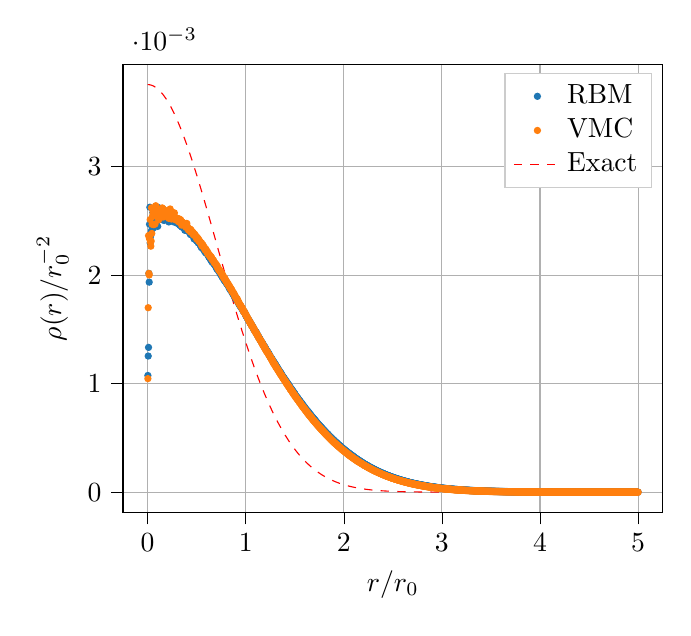
\begin{tikzpicture}

\definecolor{color0}{rgb}{0.12156862745098,0.466666666666667,0.705882352941177}
\definecolor{color1}{rgb}{1,0.498039215686275,0.0549019607843137}

\begin{axis}[
legend cell align={left},
legend style={draw=white!80.0!black},
tick align=outside,
tick pos=left,
x grid style={white!69.01960784313725!black},
xlabel={\(\displaystyle r / r_0\)},
xmajorgrids,
xmin=-0.25, xmax=5.25,
xtick style={color=black},
y grid style={white!69.01960784313725!black},
ylabel={\(\displaystyle \rho(r) / r_0^{-2}\)},
ymajorgrids,
ymin=-0.000187835169088002, ymax=0.00394453855199584,
ytick style={color=black}
]
\addplot [semithick, color0, opacity=1.0, mark=*, mark size=1, mark options={solid}, only marks]
table {%
0 nan
0.00333555703802535 0.00107531090423062
0.0066711140760507 0.00125452938826905
0.0100066711140761 0.00133418204784169
0.0133422281521014 0.00201620794543241
0.0166777851901268 0.00193555962761511
0.0200133422281521 0.00246923244675179
0.0233488992661775 0.00262609941917545
0.0266844563042028 0.00229623682674246
0.0300200133422282 0.00235417860514687
0.0333555703802535 0.00250547440685734
0.0366911274182789 0.00239649179482801
0.0400266844563042 0.00240949295207231
0.0433622414943296 0.00248042623766806
0.0466977985323549 0.00248985679610542
0.0500333555703803 0.0025178205690911
0.0533689126084056 0.00257836592466234
0.056704469646431 0.00250161717858495
0.0600400266844563 0.00243438440818876
0.0633755837224817 0.00248721497238938
0.066711140760507 0.00251577946968955
0.0700466977985324 0.00254766593296362
0.0733822548365577 0.00254164395545419
0.0767178118745831 0.00250092788123201
0.0800533689126084 0.00254328452869822
0.0833889259506338 0.0025850474137704
0.0867244829886591 0.00250667273163227
0.0900600400266845 0.00246972412983557
0.0933955970647098 0.00256483595779497
0.0967311541027352 0.00256617001758722
0.100066711140761 0.00255007989621801
0.103402268178786 0.0024495679374036
0.106737825216811 0.00254773776576906
0.110073382254837 0.00253687137874425
0.113408939292862 0.00256021976246603
0.116744496330887 0.00262083259025677
0.120080053368913 0.00256312855065773
0.123415610406938 0.00253406296240468
0.126751167444963 0.00256900512542354
0.130086724482989 0.00255406959895933
0.133422281521014 0.00256416846037993
0.136757838559039 0.00252217232415067
0.140093395597065 0.00255396499532778
0.14342895263509 0.00252951042614985
0.146764509673115 0.00254747596190791
0.150100066711141 0.00259357909864018
0.153435623749166 0.00255708187693971
0.156771180787191 0.00250865312130036
0.160106737825217 0.00260854681520354
0.163442294863242 0.00255571081840567
0.166777851901268 0.00251809138813364
0.170113408939293 0.00250444222965976
0.173448965977318 0.00254544596135212
0.176784523015344 0.00254612746262794
0.180120080053369 0.00253468775728023
0.183455637091394 0.00256060260500536
0.18679119412942 0.00254471959734167
0.190126751167445 0.00255925539718291
0.19346230820547 0.00255114635156497
0.196797865243496 0.0025231141187221
0.200133422281521 0.00256048452487469
0.203468979319546 0.00254604877808111
0.206804536357572 0.00256579886370636
0.210140093395597 0.0025512331439082
0.213475650433622 0.00254861285602315
0.216811207471648 0.00249056427735686
0.220146764509673 0.00254209652738358
0.223482321547698 0.0025307773898856
0.226817878585724 0.00250235358671573
0.230153435623749 0.00253612411785792
0.233488992661775 0.00253458826671338
0.2368245496998 0.00253298538628972
0.240160106737825 0.0025338810897209
0.243495663775851 0.0025189125982351
0.246831220813876 0.00252630642830733
0.250166777851901 0.00250571336483606
0.253502334889927 0.00252308349170178
0.256837891927952 0.00252867638425289
0.260173448965977 0.00253939984139011
0.263509006004003 0.00249168540963484
0.266844563042028 0.00251667556210974
0.270180120080053 0.00250498873323347
0.273515677118079 0.00249613180378994
0.276851234156104 0.00252505810411593
0.280186791194129 0.0025122337071652
0.283522348232155 0.00250380004731788
0.28685790527018 0.00250115920571651
0.290193462308205 0.00251071623378248
0.293529019346231 0.00248128731723463
0.296864576384256 0.00251360655021463
0.300200133422282 0.00250945703983597
0.303535690460307 0.00249583543470167
0.306871247498332 0.00250698370429853
0.310206804536358 0.00250077025837238
0.313542361574383 0.00248786329036561
0.316877918612408 0.00249994395280695
0.320213475650434 0.0024709242879097
0.323549032688459 0.0024910778807009
0.326884589726484 0.00246296655917295
0.33022014676451 0.0024622107246958
0.333555703802535 0.00245676282289569
0.33689126084056 0.00248838039640741
0.340226817878586 0.00248042929552389
0.343562374916611 0.00245290624180875
0.346897931954636 0.00245625096324017
0.350233488992662 0.00244488149082529
0.353569046030687 0.00244170031640155
0.356904603068712 0.00244494148152357
0.360240160106738 0.0024469684221143
0.363575717144763 0.00244715214759326
0.366911274182789 0.00244365143558656
0.370246831220814 0.00244002453213859
0.373582388258839 0.00246029660450182
0.376917945296865 0.00244672740465192
0.38025350233489 0.0024135610847894
0.383589059372915 0.00245034016093595
0.386924616410941 0.00243576512926823
0.390260173448966 0.00242769104490695
0.393595730486991 0.00242018319249003
0.396931287525017 0.0024104069805435
0.400266844563042 0.00241766979540656
0.403602401601067 0.00241356779955676
0.406937958639093 0.00241993117516398
0.410273515677118 0.00241779701429129
0.413609072715143 0.00241094085258938
0.416944629753169 0.00241491315625091
0.420280186791194 0.00240479687690476
0.423615743829219 0.00241445488459792
0.426951300867245 0.00241179249479557
0.43028685790527 0.00238659658183821
0.433622414943296 0.00239822964182298
0.436957971981321 0.00237426634174502
0.440293529019346 0.00237979806206892
0.443629086057372 0.00238422690691079
0.446964643095397 0.0023804638250817
0.450300200133422 0.00238032631154238
0.453635757171448 0.00236917999001243
0.456971314209473 0.00237364946745669
0.460306871247498 0.00236749273708262
0.463642428285524 0.00236246341802957
0.466977985323549 0.00237074965462151
0.470313542361574 0.00237256029631528
0.4736490993996 0.00233437319404994
0.476984656437625 0.00234615917446356
0.48032021347565 0.00234206130602351
0.483655770513676 0.00233584123484274
0.486991327551701 0.00233247190187779
0.490326884589726 0.00233328217647745
0.493662441627752 0.0023363367989061
0.496997998665777 0.00232196956496769
0.500333555703803 0.00231554264010638
0.503669112741828 0.00232248322478071
0.507004669779853 0.00231427968485679
0.510340226817879 0.00231673328046696
0.513675783855904 0.00230792539944386
0.517011340893929 0.00229750263887608
0.520346897931955 0.00230844689604456
0.52368245496998 0.00229835036372485
0.527018012008005 0.00229678064184284
0.530353569046031 0.00229287794228503
0.533689126084056 0.00228914509532329
0.537024683122081 0.0022766645137589
0.540360240160107 0.00227973642047597
0.543695797198132 0.0022742717023567
0.547031354236157 0.00225600328991081
0.550366911274183 0.00227576864409226
0.553702468312208 0.00226251954463054
0.557038025350234 0.00225296443733986
0.560373582388259 0.00224600307436052
0.563709139426284 0.00225044978586285
0.56704469646431 0.00224741219250524
0.570380253502335 0.00224237926971562
0.57371581054036 0.0022382743316343
0.577051367578386 0.00223465311543812
0.580386924616411 0.00222138339381582
0.583722481654436 0.00222998121620149
0.587058038692462 0.00221788081146184
0.590393595730487 0.00220914855078296
0.593729152768512 0.00220626981521449
0.597064709806538 0.00220531977529785
0.600400266844563 0.00220798831765761
0.603735823882588 0.00220067672525107
0.607071380920614 0.00220639357918543
0.610406937958639 0.00220011306052572
0.613742494996664 0.00218950823874675
0.61707805203469 0.00218985874347657
0.620413609072715 0.00217594323145753
0.62374916611074 0.00217954256414281
0.627084723148766 0.00216471325728261
0.630420280186791 0.00216416817913685
0.633755837224817 0.00216275504876566
0.637091394262842 0.00215398206292472
0.640426951300867 0.00214867230183961
0.643762508338893 0.00215668412664128
0.647098065376918 0.00213685518508587
0.650433622414943 0.00214237375199661
0.653769179452969 0.00212780429478381
0.657104736490994 0.0021264929574447
0.660440293529019 0.00211822405832399
0.663775850567045 0.00212475345021867
0.66711140760507 0.00211592959041349
0.670446964643095 0.00212263957541466
0.673782521681121 0.00211467182091456
0.677118078719146 0.00210267828719064
0.680453635757171 0.00210501187563609
0.683789192795197 0.00210442800431836
0.687124749833222 0.00209335433170656
0.690460306871247 0.00208876593876896
0.693795863909273 0.00209198144094903
0.697131420947298 0.00207456647459478
0.700466977985324 0.00207553292116921
0.703802535023349 0.00207106620773233
0.707138092061374 0.00205585261809862
0.7104736490994 0.00206497663328794
0.713809206137425 0.00205859799301526
0.71714476317545 0.00205243450487501
0.720480320213476 0.00204719550353293
0.723815877251501 0.00204153941191373
0.727151434289526 0.00203325715775329
0.730486991327552 0.00203492441468717
0.733822548365577 0.0020323227975509
0.737158105403602 0.00202714925938547
0.740493662441628 0.00201731342427235
0.743829219479653 0.00200853433532284
0.747164776517678 0.00201187892752236
0.750500333555704 0.00200121465981218
0.753835890593729 0.00200000052555275
0.757171447631754 0.00199844139026756
0.76050700466978 0.00198178740556168
0.763842561707805 0.00199008352185904
0.767178118745831 0.00198579162124154
0.770513675783856 0.00198346743106746
0.773849232821881 0.00197401714929591
0.777184789859907 0.00195758783038716
0.780520346897932 0.00196057938683212
0.783855903935957 0.00195721837206912
0.787191460973983 0.00194540995121714
0.790527018012008 0.00194713804337609
0.793862575050033 0.00194265888675086
0.797198132088059 0.00193980218699112
0.800533689126084 0.00193151476599619
0.803869246164109 0.00193002764816944
0.807204803202135 0.00191896652495557
0.81054036024016 0.00192739465334357
0.813875917278185 0.00191721875185004
0.817211474316211 0.00190953898474306
0.820547031354236 0.00190904882013584
0.823882588392261 0.00190470275731669
0.827218145430287 0.0018973340826536
0.830553702468312 0.00188341424917998
0.833889259506338 0.00188622149583327
0.837224816544363 0.00188110424442673
0.840560373582388 0.00187171896921359
0.843895930620414 0.00186494291387751
0.847231487658439 0.00186791851157197
0.850567044696464 0.00186114640423097
0.85390260173449 0.00186005355890343
0.857238158772515 0.00184678150524435
0.86057371581054 0.00184611408495034
0.863909272848566 0.00184202222505741
0.867244829886591 0.00183126825594197
0.870580386924616 0.00182808852135899
0.873915943962642 0.0018277314236281
0.877251501000667 0.00181769087281037
0.880587058038692 0.00181181514782165
0.883922615076718 0.00180822454379741
0.887258172114743 0.0018012653178743
0.890593729152768 0.0018023186577918
0.893929286190794 0.00179285107082597
0.897264843228819 0.00179536743531795
0.900600400266845 0.00177906427729365
0.90393595730487 0.00177845080043163
0.907271514342895 0.00177055769633301
0.910607071380921 0.00176962412150649
0.913942628418946 0.00176686661296532
0.917278185456971 0.00176442463777906
0.920613742494997 0.00175374189209109
0.923949299533022 0.00175007390385803
0.927284856571047 0.0017445394937013
0.930620413609073 0.00173394188370703
0.933955970647098 0.00173450574868464
0.937291527685123 0.00172538276819405
0.940627084723149 0.00172632445889526
0.943962641761174 0.00171630749946644
0.947298198799199 0.00171091702602186
0.950633755837225 0.00170847232226287
0.95396931287525 0.00170216587348232
0.957304869913275 0.00170076206892511
0.960640426951301 0.00169784578955968
0.963975983989326 0.00168927921378708
0.967311541027352 0.00168691475842224
0.970647098065377 0.00167672065321504
0.973982655103402 0.00167136412260179
0.977318212141428 0.001672661315531
0.980653769179453 0.00166490562962515
0.983989326217478 0.00165812261833398
0.987324883255504 0.00166108673204219
0.990660440293529 0.00164913960272464
0.993995997331554 0.00164833821312875
0.99733155436958 0.00164168509553603
1.00066711140761 0.00162976111961682
1.00400266844563 0.00162397847873577
1.00733822548366 0.00162180702078706
1.01067378252168 0.00161898071386341
1.01400933955971 0.00161181055847016
1.01734489659773 0.00160300602780544
1.02068045363576 0.00160186329314473
1.02401601067378 0.00159190106794841
1.02735156771181 0.00158962699524149
1.03068712474983 0.00158193755732162
1.03402268178786 0.00158360510959565
1.03735823882588 0.00157784382489
1.04069379586391 0.00157333886363509
1.04402935290193 0.00156213818030036
1.04736490993996 0.00155852426117538
1.05070046697799 0.00155566882075357
1.05403602401601 0.00155102527798174
1.05737158105404 0.00154796445476716
1.06070713809206 0.00153450643083996
1.06404269513009 0.00153729413807292
1.06737825216811 0.00153096689917631
1.07071380920614 0.00152625738530752
1.07404936624416 0.00151800565772219
1.07738492328219 0.00151586827631268
1.08072048032021 0.00150445633856092
1.08405603735824 0.00149918107106212
1.08739159439626 0.00149828952836909
1.09072715143429 0.0014936516200094
1.09406270847231 0.00148657854418058
1.09739826551034 0.00148027901168104
1.10073382254837 0.00147806371563336
1.10406937958639 0.00147714694314496
1.10740493662442 0.00147167798549199
1.11074049366244 0.00146731951918361
1.11407605070047 0.00145392433023928
1.11741160773849 0.0014535166013243
1.12074716477652 0.00144970507363928
1.12408272181454 0.00143991334543077
1.12741827885257 0.00144149271366194
1.13075383589059 0.00143209480982908
1.13408939292862 0.0014219885972086
1.13742494996664 0.00141978103419674
1.14076050700467 0.00141591703975427
1.1440960640427 0.00141413801973733
1.14743162108072 0.00140562988306789
1.15076717811875 0.00140118062516389
1.15410273515677 0.00139564545612464
1.1574382921948 0.00138979053116931
1.16077384923282 0.00138590211322896
1.16410940627085 0.00138118343421758
1.16744496330887 0.00137555819080427
1.1707805203469 0.00137321121097146
1.17411607738492 0.00136760840626005
1.17745163442295 0.00136352835328231
1.18078719146097 0.00135275374845233
1.184122748499 0.00135167213490397
1.18745830553702 0.00134300168686914
1.19079386257505 0.00134105132335211
1.19412941961308 0.00134107483937563
1.1974649766511 0.00132839386352261
1.20080053368913 0.00132628730767676
1.20413609072715 0.00132412729082276
1.20747164776518 0.00131187645851034
1.2108072048032 0.00130628647978222
1.21414276184123 0.00130476483144246
1.21747831887925 0.00130096409370751
1.22081387591728 0.0013002865874434
1.2241494329553 0.00129139792063426
1.22748498999333 0.00128583545261816
1.23082054703135 0.00128287428918611
1.23415610406938 0.00127870882873793
1.2374916611074 0.00127456567129797
1.24082721814543 0.00126555182234851
1.24416277518346 0.00126049092859587
1.24749833222148 0.00125316740159133
1.25083388925951 0.00124506665231182
1.25416944629753 0.00124594217395491
1.25750500333556 0.00124121747067311
1.26084056037358 0.00123751489584176
1.26417611741161 0.00123091074245868
1.26751167444963 0.00122745548237699
1.27084723148766 0.00122085516342803
1.27418278852568 0.00121663809780584
1.27751834556371 0.00121033106475076
1.28085390260173 0.00120579536893794
1.28418945963976 0.00120377268230549
1.28752501667779 0.00119755923430846
1.29086057371581 0.00119244449348197
1.29419613075384 0.00118987482968068
1.29753168779186 0.00118335174303976
1.30086724482989 0.00118030159326257
1.30420280186791 0.00117597762461989
1.30753835890594 0.00116883541886357
1.31087391594396 0.00116159857789679
1.31420947298199 0.00115710886366716
1.31754503002001 0.00115561548783001
1.32088058705804 0.00114884584274764
1.32421614409606 0.00114409685259938
1.32755170113409 0.00114114035471982
1.33088725817211 0.00113119925203353
1.33422281521014 0.00113033545929252
1.33755837224817 0.00112166556601532
1.34089392928619 0.00111785649667666
1.34422948632422 0.00111772285932875
1.34756504336224 0.00110958856950993
1.35090060040027 0.00110740251279451
1.35423615743829 0.00110412529103924
1.35757171447632 0.00109805171954495
1.36090727151434 0.00109312573659908
1.36424282855237 0.00108897933889661
1.36757838559039 0.0010827483113969
1.37091394262842 0.00107437089335655
1.37424949966644 0.00107165672397531
1.37758505670447 0.00106712587652535
1.38092061374249 0.00106308528335628
1.38425617078052 0.0010587298775233
1.38759172781855 0.00105402808788519
1.39092728485657 0.00105209141808197
1.3942628418946 0.00104472486009505
1.39759839893262 0.00104006561980007
1.40093395597065 0.00103674235496153
1.40426951300867 0.00103083819551774
1.4076050700467 0.00102963375999791
1.41094062708472 0.00102217006808522
1.41427618412275 0.00101886948317995
1.41761174116077 0.00101392962767383
1.4209472981988 0.00101082124474574
1.42428285523682 0.00100403496933776
1.42761841227485 0.00100283261063218
1.43095396931288 0.000997003057642352
1.4342895263509 0.00099323969439294
1.43762508338893 0.000989516884433125
1.44096064042695 0.000982506682485341
1.44429619746498 0.000979702987107349
1.447631754503 0.000972858476448531
1.45096731154103 0.000965882735601562
1.45430286857905 0.000964966184674042
1.45763842561708 0.000959790064237156
1.4609739826551 0.000954721164587461
1.46430953969313 0.000949505240111731
1.46764509673115 0.000948533266794936
1.47098065376918 0.000945110008557998
1.4743162108072 0.00094019159386131
1.47765176784523 0.000934397427162877
1.48098732488326 0.00093160410970353
1.48432288192128 0.000923292179410922
1.48765843895931 0.000916559885362912
1.49099399599733 0.000919951263764905
1.49432955303536 0.000913339734740981
1.49766511007338 0.000910544505722574
1.50100066711141 0.000906708349654112
1.50433622414943 0.000898874962916127
1.50767178118746 0.00089185810455248
1.51100733822548 0.000888182524378956
1.51434289526351 0.000885163636760137
1.51767845230153 0.00088082259848005
1.52101400933956 0.000876242173453332
1.52434956637759 0.00087421882176394
1.52768512341561 0.000869755255621669
1.53102068045364 0.000865499184162552
1.53435623749166 0.0008617207542222
1.53769179452969 0.000857498898036634
1.54102735156771 0.000852455753827806
1.54436290860574 0.000845930740834129
1.54769846564376 0.000844485195086062
1.55103402268179 0.000839700657999839
1.55436957971981 0.000839183973882291
1.55770513675784 0.000831184280945085
1.56104069379586 0.000827728469645924
1.56437625083389 0.000823614207019668
1.56771180787191 0.00082270695375158
1.57104736490994 0.000816510853098369
1.57438292194797 0.000814024088064949
1.57771847898599 0.000810786828149034
1.58105403602402 0.000803609154254117
1.58438959306204 0.000800332360084756
1.58772515010007 0.000794781328670524
1.59106070713809 0.000791097164706702
1.59439626417612 0.000788938930731183
1.59773182121414 0.000786434056877917
1.60106737825217 0.000779656411343459
1.60440293529019 0.000777341322031401
1.60773849232822 0.000771362144008167
1.61107404936624 0.000767367840790819
1.61440960640427 0.000762973028489565
1.61774516344229 0.000759730182337943
1.62108072048032 0.0007576183778712
1.62441627751835 0.000750966170492457
1.62775183455637 0.000750536101864572
1.6310873915944 0.000746693842495878
1.63442294863242 0.000742416862117074
1.63775850567045 0.000739550466602467
1.64109406270847 0.000736615333711419
1.6444296197465 0.000730376764306553
1.64776517678452 0.000728518481560625
1.65110073382255 0.000722262376402336
1.65443629086057 0.000719198525540478
1.6577718478986 0.000716137498366866
1.66110740493662 0.000710777715401869
1.66444296197465 0.000708833608262719
1.66777851901268 0.000705110034861462
1.6711140760507 0.000699878950647381
1.67444963308873 0.000696931218064326
1.67778519012675 0.000692625050287678
1.68112074716478 0.000689256272938827
1.6844563042028 0.000685884124530857
1.68779186124083 0.000682417027378119
1.69112741827885 0.000679030486552158
1.69446297531688 0.000674872902704055
1.6977985323549 0.000673342302415498
1.70113408939293 0.000666902227824627
1.70446964643095 0.000663376956828543
1.70780520346898 0.000663681438325793
1.711140760507 0.000658591784686583
1.71447631754503 0.000652883421398359
1.71781187458306 0.000650022688038467
1.72114743162108 0.000645192869733814
1.72448298865911 0.000643699095299648
1.72781854569713 0.000638668061623041
1.73115410273516 0.000636007683986462
1.73448965977318 0.000632223690797158
1.73782521681121 0.000627680320497906
1.74116077384923 0.000625350725649948
1.74449633088726 0.000621929660166344
1.74783188792528 0.000618346065536611
1.75116744496331 0.000616243041839947
1.75450300200133 0.000610570731627339
1.75783855903936 0.00060933987735134
1.76117411607738 0.000604636097665027
1.76450967311541 0.000601859809095956
1.76784523015344 0.000598915124466446
1.77118078719146 0.00059681208835031
1.77451634422949 0.000592779142941931
1.77785190126751 0.000589174717970315
1.78118745830554 0.000585067061130751
1.78452301534356 0.000581397973889875
1.78785857238159 0.000579400278821452
1.79119412941961 0.000573879625173662
1.79452968645764 0.000573766140155557
1.79786524349566 0.000568190717178483
1.80120080053369 0.000566580553330332
1.80453635757171 0.000561797938884806
1.80787191460974 0.00056004525605388
1.81120747164777 0.000556884198838397
1.81454302868579 0.000553196328309467
1.81787858572382 0.000548976641968059
1.82121414276184 0.000545628773754542
1.82454969979987 0.000542938404931631
1.82788525683789 0.000540162567742957
1.83122081387592 0.000536890178645886
1.83455637091394 0.00053504567551303
1.83789192795197 0.000534812522681186
1.84122748498999 0.000529653366565585
1.84456304202802 0.000525918100375099
1.84789859906604 0.000521264443347571
1.85123415610407 0.000518054730452175
1.85456971314209 0.000517259621519855
1.85790527018012 0.000512360291784223
1.86124082721815 0.000509795670430758
1.86457638425617 0.000506123125241197
1.8679119412942 0.000505711586095498
1.87124749833222 0.000501113721119454
1.87458305537025 0.000498845132296737
1.87791861240827 0.000495214399996984
1.8812541694463 0.000492902101420471
1.88458972648432 0.000488098011366492
1.88792528352235 0.000485758309221798
1.89126084056037 0.000483986180904423
1.8945963975984 0.000480369797768516
1.89793195463642 0.000478477443477415
1.90126751167445 0.0004749444278159
1.90460306871247 0.00047181908101397
1.9079386257505 0.000467807219284103
1.91127418278853 0.000466621222972157
1.91460973982655 0.000463300745073976
1.91794529686458 0.000461023932094143
1.9212808539026 0.000457845060225266
1.92461641094063 0.000456663720441327
1.92795196797865 0.000451772373546393
1.93128752501668 0.000450805527140737
1.9346230820547 0.000447851754844384
1.93795863909273 0.000444600262339532
1.94129419613075 0.000439636712731549
1.94462975316878 0.00043910213266051
1.9479653102068 0.000434668512103237
1.95130086724483 0.0004331654070186
1.95463642428286 0.000431254067135961
1.95797198132088 0.000428148620016506
1.96130753835891 0.000426382038564835
1.96464309539693 0.000422725447196462
1.96797865243496 0.000420790687756215
1.97131420947298 0.000416214342048488
1.97464976651101 0.000415606122178512
1.97798532354903 0.000411495269729342
1.98132088058706 0.000409488707110687
1.98465643762508 0.00040695770542489
1.98799199466311 0.000405518550198778
1.99132755170113 0.000401262768295446
1.99466310873916 0.000397881131973935
1.99799866577718 0.000397404392397804
2.00133422281521 0.000394741156822714
2.00466977985324 0.000391942098382889
2.00800533689126 0.000389117409655179
2.01134089392929 0.000386927368569912
2.01467645096731 0.000385311192807483
2.01801200800534 0.000381945791447236
2.02134756504336 0.000379328612913439
2.02468312208139 0.000378398395975901
2.02801867911941 0.000374105689363333
2.03135423615744 0.000372526804325137
2.03468979319546 0.000369878341601014
2.03802535023349 0.000368032034629454
2.04136090727151 0.000366015416403907
2.04469646430954 0.000363048480793908
2.04803202134757 0.000360354198355515
2.05136757838559 0.000358666307084803
2.05470313542362 0.000357740792379367
2.05803869246164 0.000354423619710023
2.06137424949967 0.000351963640956005
2.06470980653769 0.00034854948074364
2.06804536357572 0.000347293159009529
2.07138092061374 0.000345353922543202
2.07471647765177 0.000341822092902384
2.07805203468979 0.000339849692051419
2.08138759172782 0.000339001104219082
2.08472314876584 0.000336194835884362
2.08805870580387 0.000335484712622502
2.09139426284189 0.000332489358832834
2.09472981987992 0.000329767209268237
2.09806537691795 0.000328320420723854
2.10140093395597 0.000324522725999082
2.104736490994 0.000323044827255802
2.10807204803202 0.000320235752044415
2.11140760507005 0.000318064961841919
2.11474316210807 0.000315458168033084
2.1180787191461 0.000314816951356639
2.12141427618412 0.000311375811182588
2.12474983322215 0.000310380396096751
2.12808539026017 0.000308329462313382
2.1314209472982 0.00030620249238631
2.13475650433622 0.000304030856799345
2.13809206137425 0.000302522926130695
2.14142761841227 0.000299644953227558
2.1447631754503 0.000296872701591664
2.14809873248833 0.000295283384668918
2.15143428952635 0.000294164293642484
2.15476984656438 0.000291476329061658
2.1581054036024 0.000290774668283025
2.16144096064043 0.000287636311245235
2.16477651767845 0.000285509004253776
2.16811207471648 0.000284144225517204
2.1714476317545 0.000281433251248628
2.17478318879253 0.000281186560271368
2.17811874583055 0.000276821147253466
2.18145430286858 0.000277299327097337
2.1847898599066 0.000274851664404082
2.18812541694463 0.000272579213509827
2.19146097398266 0.000269791185934107
2.19479653102068 0.000268499890396125
2.19813208805871 0.00026704103396971
2.20146764509673 0.000264355492537228
2.20480320213476 0.000262875324980288
2.20813875917278 0.000260723627203615
2.21147431621081 0.000259642130994891
2.21480987324883 0.000257896884647713
2.21814543028686 0.000255907663011948
2.22148098732488 0.000254049219460539
2.22481654436291 0.000252171757826713
2.22815210140093 0.000250187516067363
2.23148765843896 0.000248648072571593
2.23482321547698 0.000247359834937773
2.23815877251501 0.000246227435374459
2.24149432955304 0.000243252866123722
2.24482988659106 0.000242401517831312
2.24816544362909 0.000239702690651563
2.25150100066711 0.000238730231113507
2.25483655770514 0.00023732361900869
2.25817211474316 0.000234912686020153
2.26150767178119 0.000232413176872401
2.26484322881921 0.000231944848844363
2.26817878585724 0.000229647712834303
2.27151434289526 0.000228269661176045
2.27484989993329 0.000227618078552054
2.27818545697131 0.000225392247455459
2.28152101400934 0.000223434336687765
2.28485657104736 0.0002227266857621
2.28819212808539 0.000219942860341359
2.29152768512342 0.000219060382554578
2.29486324216144 0.000217911766252445
2.29819879919947 0.000215796389165869
2.30153435623749 0.000214307438017942
2.30486991327552 0.000211992562146818
2.30820547031354 0.000211043852010747
2.31154102735157 0.000209366062589415
2.31487658438959 0.000208225075086963
2.31821214142762 0.000205844594180905
2.32154769846564 0.000203948634048067
2.32488325550367 0.000203862966968361
2.32821881254169 0.000202092195614035
2.33155436957972 0.000199852409472682
2.33488992661775 0.000199063822253623
2.33822548365577 0.00019709069551505
2.3415610406938 0.000195357108453363
2.34489659773182 0.000194180525265815
2.34823215476985 0.000193459673904957
2.35156771180787 0.000191060011156433
2.3549032688459 0.00019105885006213
2.35823882588392 0.000188026865164281
2.36157438292195 0.000187339848957786
2.36490993995997 0.000186629931549265
2.368245496998 0.000184483049227171
2.37158105403602 0.000182816531190792
2.37491661107405 0.000181344596514384
2.37825216811207 0.000180171741968876
2.3815877251501 0.000179661436297552
2.38492328218813 0.000178153462268161
2.38825883922615 0.000176728367348481
2.39159439626418 0.000175276011361544
2.3949299533022 0.000172994625363108
2.39826551034023 0.000172331052254623
2.40160106737825 0.000172502285177682
2.40493662441628 0.000170650944065946
2.4082721814543 0.000168143590072133
2.41160773849233 0.000167485073075495
2.41494329553035 0.000165731008918728
2.41827885256838 0.000164898735372284
2.4216144096064 0.000163747732561866
2.42494996664443 0.000162278265004869
2.42828552368245 0.000161225081340081
2.43162108072048 0.000160253276037259
2.43495663775851 0.000158552363107376
2.43829219479653 0.000157665083512863
2.44162775183456 0.000156439557306984
2.44496330887258 0.000154767819094643
2.44829886591061 0.000153607242020522
2.45163442294863 0.000152523397780664
2.45496997998666 0.000151734033120347
2.45830553702468 0.000150280899777142
2.46164109406271 0.000149250677951619
2.46497665110073 0.000148440755361984
2.46831220813876 0.000147274654754127
2.47164776517678 0.00014568607086499
2.47498332221481 0.000144819696463735
2.47831887925284 0.000143840908715223
2.48165443629086 0.000142575787030382
2.48498999332889 0.000141614973280009
2.48832555036691 0.000139865297484984
2.49166110740494 0.000139246019673217
2.49499666444296 0.000137651944713935
2.49833222148099 0.000137007015696222
2.50166777851901 0.000135457631479867
2.50500333555704 0.000134630656635107
2.50833889259506 0.000133941021142323
2.51167444963309 0.000132581011726083
2.51501000667111 0.000132035383861891
2.51834556370914 0.000130065725965311
2.52168112074716 0.000129119489823106
2.52501667778519 0.000128368258359199
2.52835223482322 0.000127664519948468
2.53168779186124 0.000126779871324192
2.53502334889927 0.00012553857646817
2.53835890593729 0.000124238685560625
2.54169446297532 0.000123614036015192
2.54503002001334 0.000122725021757103
2.54836557705137 0.000121133734551622
2.55170113408939 0.000120454665535038
2.55503669112742 0.000119808049559116
2.55837224816544 0.000118892956603296
2.56170780520347 0.000118273309453317
2.56504336224149 0.000116647287952608
2.56837891927952 0.000115535618464589
2.57171447631755 0.000114737745265787
2.57505003335557 0.000114102992154092
2.5783855903936 0.000112888668202525
2.58172114743162 0.000111695491910033
2.58505670446965 0.00011114664150917
2.58839226150767 0.000110770782616294
2.5917278185457 0.000108612702319198
2.59506337558372 0.000108369498607324
2.59839893262175 0.000107851641840279
2.60173448965977 0.000107053292295004
2.6050700466978 0.000105561441495343
2.60840560373582 0.000104832397504354
2.61174116077385 0.000104249968184299
2.61507671781187 0.000102987006600004
2.6184122748499 0.000102494446816299
2.62174783188793 0.00010115669615559
2.62508338892595 0.000100464887452599
2.62841894596398 9.94703224478191e-05
2.631754503002 9.87191356608306e-05
2.63509006004003 9.87622783278884e-05
2.63842561707805 9.78974534958238e-05
2.64176117411608 9.63109637210941e-05
2.6450967311541 9.5599683166848e-05
2.64843228819213 9.49439850723833e-05
2.65176784523015 9.4382305003399e-05
2.65510340226818 9.35586809422072e-05
2.6584389593062 9.26026166508839e-05
2.66177451634423 9.13521646008131e-05
2.66511007338225 9.09692398041905e-05
2.66844563042028 9.062070633851e-05
2.67178118745831 8.94420629426627e-05
2.67511674449633 8.90542031509825e-05
2.67845230153436 8.73491694970316e-05
2.68178785857238 8.69476472462406e-05
2.68512341561041 8.61302421041507e-05
2.68845897264843 8.59549986589777e-05
2.69179452968646 8.50458714626915e-05
2.69513008672448 8.44929021605211e-05
2.69846564376251 8.39374763749196e-05
2.70180120080053 8.26836126268838e-05
2.70513675783856 8.24065347955929e-05
2.70847231487658 8.18794147225641e-05
2.71180787191461 8.08096355751316e-05
2.71514342895264 8.00377920034194e-05
2.71847898599066 7.95341804011862e-05
2.72181454302869 7.8469184956029e-05
2.72515010006671 7.80809405192438e-05
2.72848565710474 7.75194590604138e-05
2.73182121414276 7.69302932843961e-05
2.73515677118079 7.66041743635259e-05
2.73849232821881 7.53294021978863e-05
2.74182788525684 7.45271601001649e-05
2.74516344229486 7.45117962114834e-05
2.74849899933289 7.31926181403615e-05
2.75183455637091 7.35640366063635e-05
2.75517011340894 7.2496334928633e-05
2.75850567044696 7.19574022360839e-05
2.76184122748499 7.08138661026804e-05
2.76517678452302 7.0491092938206e-05
2.76851234156104 6.98463002614189e-05
2.77184789859907 6.93126275681385e-05
2.77518345563709 6.85783377498974e-05
2.77851901267512 6.76394556700535e-05
2.78185456971314 6.70936889807644e-05
2.78519012675117 6.6646219089272e-05
2.78852568378919 6.62722411251137e-05
2.79186124082722 6.57325537865309e-05
2.79519679786524 6.51281324620399e-05
2.79853235490327 6.45139288726312e-05
2.80186791194129 6.35113122644713e-05
2.80520346897932 6.3328944000744e-05
2.80853902601734 6.28338037327167e-05
2.81187458305537 6.23905146685479e-05
2.8152101400934 6.19126679090071e-05
2.81854569713142 6.1089024526725e-05
2.82188125416945 6.06091493959661e-05
2.82521681120747 5.98415851473667e-05
2.8285523682455 5.95078818513393e-05
2.83188792528352 5.8822517914555e-05
2.83522348232155 5.82262870779159e-05
2.83855903935957 5.79707395342671e-05
2.8418945963976 5.76957387408557e-05
2.84523015343562 5.68969775510509e-05
2.84856571047365 5.67298959410534e-05
2.85190126751167 5.58833645396879e-05
2.8552368245497 5.5447626286337e-05
2.85857238158773 5.48295351631174e-05
2.86190793862575 5.42984066634129e-05
2.86524349566378 5.41596708687156e-05
2.8685790527018 5.31260676839789e-05
2.87191460973983 5.28286698347451e-05
2.87525016677785 5.25264783511535e-05
2.87858572381588 5.18860069744681e-05
2.8819212808539 5.11753740912651e-05
2.88525683789193 5.10314887631941e-05
2.88859239492995 5.04816398038011e-05
2.89192795196798 5.02870535526459e-05
2.895263509006 4.96936045068722e-05
2.89859906604403 4.91627955396243e-05
2.90193462308205 4.89319263277144e-05
2.90527018012008 4.81328940887025e-05
2.90860573715811 4.7998048593878e-05
2.91194129419613 4.79572859926792e-05
2.91527685123416 4.68272562945183e-05
2.91861240827218 4.64115305126985e-05
2.92194796531021 4.63759262896942e-05
2.92528352234823 4.54716842918166e-05
2.92861907938626 4.51717138358925e-05
2.93195463642428 4.47660583744766e-05
2.93529019346231 4.47645838224465e-05
2.93862575050033 4.39608409880704e-05
2.94196130753836 4.36160882491411e-05
2.94529686457638 4.36104463717718e-05
2.94863242161441 4.31068230051961e-05
2.95196797865243 4.24172722291258e-05
2.95530353569046 4.21629042635253e-05
2.95863909272849 4.1824609071147e-05
2.96197464976651 4.14347742251076e-05
2.96531020680454 4.08293440907181e-05
2.96864576384256 4.02733641230571e-05
2.97198132088059 4.00891025638774e-05
2.97531687791861 3.97287491116645e-05
2.97865243495664 3.93553002541739e-05
2.98198799199466 3.90195241549783e-05
2.98532354903269 3.83555858502259e-05
2.98865910607071 3.8426284596351e-05
2.99199466310874 3.80506477410594e-05
2.99533022014676 3.76303611060808e-05
2.99866577718479 3.72486597700824e-05
3.00200133422282 3.66687656064271e-05
3.00533689126084 3.66841108069771e-05
3.00867244829887 3.63642560987915e-05
3.01200800533689 3.56566997470466e-05
3.01534356237492 3.54320199214822e-05
3.01867911941294 3.51069321964026e-05
3.02201467645097 3.49419232709813e-05
3.02535023348899 3.44263734857635e-05
3.02868579052702 3.41456008888703e-05
3.03202134756504 3.39080579690164e-05
3.03535690460307 3.34392560907847e-05
3.03869246164109 3.3211050588819e-05
3.04202801867912 3.26566768187054e-05
3.04536357571714 3.25561537299877e-05
3.04869913275517 3.2372539517685e-05
3.0520346897932 3.17598122623317e-05
3.05537024683122 3.17597104485983e-05
3.05870580386925 3.13537344469703e-05
3.06204136090727 3.09356277964496e-05
3.0653769179453 3.06266405218988e-05
3.06871247498332 3.06375946490707e-05
3.07204803202135 3.02503727740148e-05
3.07538358905937 2.99859818815021e-05
3.0787191460974 2.96664969217721e-05
3.08205470313542 2.93416068136052e-05
3.08539026017345 2.85662481480157e-05
3.08872581721147 2.87731572937731e-05
3.0920613742495 2.83048450788097e-05
3.09539693128752 2.81504360478077e-05
3.09873248832555 2.7725007549977e-05
3.10206804536358 2.75514488087855e-05
3.1054036024016 2.77340056631061e-05
3.10873915943963 2.72276235127423e-05
3.11207471647765 2.66895827268612e-05
3.11541027351568 2.627992386103e-05
3.1187458305537 2.61862246871614e-05
3.12208138759173 2.59973339251734e-05
3.12541694462975 2.57783660434411e-05
3.12875250166778 2.56276948746549e-05
3.1320880587058 2.52597121616799e-05
3.13542361574383 2.48897884226943e-05
3.13875917278185 2.48322606867451e-05
3.14209472981988 2.44515714037096e-05
3.14543028685791 2.41540635694148e-05
3.14876584389593 2.4103922372633e-05
3.15210140093396 2.37996688117378e-05
3.15543695797198 2.38272812542106e-05
3.15877251501001 2.32152354316929e-05
3.16210807204803 2.31018716973739e-05
3.16544362908606 2.25873544786012e-05
3.16877918612408 2.27628325632774e-05
3.17211474316211 2.24435035622751e-05
3.17545030020013 2.20457734855248e-05
3.17878585723816 2.19841398304466e-05
3.18212141427618 2.17269792382299e-05
3.18545697131421 2.14144497317208e-05
3.18879252835223 2.13479064889055e-05
3.19212808539026 2.08851353929023e-05
3.19546364242829 2.0930603066993e-05
3.19879919946631 2.04707320378149e-05
3.20213475650434 2.05315620060526e-05
3.20547031354236 2.03289492214367e-05
3.20880587058039 1.99997079462241e-05
3.21214142761841 1.97429074396132e-05
3.21547698465644 1.9610941190859e-05
3.21881254169446 1.94571545397577e-05
3.22214809873249 1.93740628730302e-05
3.22548365577051 1.90344496874557e-05
3.22881921280854 1.89127080599565e-05
3.23215476984656 1.86423595383814e-05
3.23549032688459 1.85351798084602e-05
3.23882588392261 1.81020285201305e-05
3.24216144096064 1.81843070129178e-05
3.24549699799867 1.81329399955782e-05
3.24883255503669 1.7829167037108e-05
3.25216811207472 1.76674312107234e-05
3.25550366911274 1.75006762366166e-05
3.25883922615077 1.71875537210986e-05
3.26217478318879 1.70701669357288e-05
3.26551034022682 1.68400949604801e-05
3.26884589726484 1.67626384675184e-05
3.27218145430287 1.66024049920047e-05
3.27551701134089 1.63864769062607e-05
3.27885256837892 1.61038812545784e-05
3.28218812541694 1.60543228563085e-05
3.28552368245497 1.57973088442898e-05
3.288859239493 1.56773497901295e-05
3.29219479653102 1.54897750806936e-05
3.29553035356905 1.53502956669155e-05
3.29886591060707 1.52073174175159e-05
3.3022014676451 1.50798795446197e-05
3.30553702468312 1.48357672094998e-05
3.30887258172115 1.47758215390527e-05
3.31220813875917 1.45864964297116e-05
3.3155436957972 1.44300086846124e-05
3.31887925283522 1.42210801621934e-05
3.32221480987325 1.42741968298504e-05
3.32555036691127 1.39576399442575e-05
3.3288859239493 1.38706632308574e-05
3.33222148098732 1.37439608536281e-05
3.33555703802535 1.34684482939725e-05
3.33889259506338 1.36622657095911e-05
3.3422281521014 1.33599350394747e-05
3.34556370913943 1.29759434959246e-05
3.34889926617745 1.29844219812097e-05
3.35223482321548 1.27921567978842e-05
3.3555703802535 1.27114865506395e-05
3.35890593729153 1.24266283480488e-05
3.36224149432955 1.24998782639202e-05
3.36557705136758 1.23170338211649e-05
3.3689126084056 1.23149680003512e-05
3.37224816544363 1.19495821979036e-05
3.37558372248165 1.19466273168812e-05
3.37891927951968 1.18718804319724e-05
3.3822548365577 1.16567418454793e-05
3.38559039359573 1.15925555658593e-05
3.38892595063376 1.14752984749136e-05
3.39226150767178 1.11770589210707e-05
3.39559706470981 1.12979565871591e-05
3.39893262174783 1.10293236812863e-05
3.40226817878586 1.10047797508607e-05
3.40560373582388 1.09060404890658e-05
3.40893929286191 1.06426010091911e-05
3.41227484989993 1.05868694529632e-05
3.41561040693796 1.03713577556003e-05
3.41894596397598 1.0469174082942e-05
3.42228152101401 1.01901659614512e-05
3.42561707805203 1.01684619843696e-05
3.42895263509006 1.00230234784399e-05
3.43228819212809 9.78960833573225e-06
3.43562374916611 9.76300673770699e-06
3.43895930620414 9.66399055855773e-06
3.44229486324216 9.65200202763189e-06
3.44563042028019 9.38895529163987e-06
3.44896597731821 9.30727331441822e-06
3.45230153435624 9.25918250659125e-06
3.45563709139426 9.19673272367077e-06
3.45897264843229 9.13517312111735e-06
3.46230820547031 9.05902959012377e-06
3.46564376250834 8.95294710082044e-06
3.46897931954636 8.84659288351711e-06
3.47231487658439 8.77982551979461e-06
3.47565043362241 8.67335301436009e-06
3.47898599066044 8.55343386149325e-06
3.48232154769847 8.39202831163451e-06
3.48565710473649 8.31508776107819e-06
3.48899266177452 8.26119444738445e-06
3.49232821881254 8.29070783406553e-06
3.49566377585057 8.053135219634e-06
3.49899933288859 8.07834237408951e-06
3.50233488992662 7.90788353108191e-06
3.50567044696464 7.84822439044255e-06
3.50900600400267 7.83897876654334e-06
3.51234156104069 7.70562108356661e-06
3.51567711807872 7.52113116055213e-06
3.51901267511674 7.50816800361918e-06
3.52234823215477 7.3919010370608e-06
3.5256837891928 7.29498885084342e-06
3.52901934623082 7.27720253332696e-06
3.53235490326885 7.16646373563499e-06
3.53569046030687 7.11211550800092e-06
3.5390260173449 7.13549134697026e-06
3.54236157438292 6.8854523603171e-06
3.54569713142095 6.80731713430163e-06
3.54903268845897 6.78692871249067e-06
3.552368245497 6.69107621952577e-06
3.55570380253502 6.57033715230196e-06
3.55903935957305 6.56007382182327e-06
3.56237491661107 6.40135597550983e-06
3.5657104736491 6.3624105818761e-06
3.56904603068712 6.29057035511276e-06
3.57238158772515 6.22883060385487e-06
3.57571714476318 6.21331625098795e-06
3.5790527018012 6.2243114720127e-06
3.58238825883923 5.99256309700284e-06
3.58572381587725 6.02809949124847e-06
3.58905937291528 5.9381091560012e-06
3.5923949299533 5.86404782078107e-06
3.59573048699133 5.68152470215233e-06
3.59906604402935 5.48796870618221e-06
3.60240160106738 5.61778653413349e-06
3.6057371581054 5.54405716047808e-06
3.60907271514343 5.42833959498818e-06
3.61240827218145 5.43405808039713e-06
3.61574382921948 5.4235792101881e-06
3.6190793862575 5.34370915350349e-06
3.62241494329553 5.24908011739882e-06
3.62575050033356 5.20241711151386e-06
3.62908605737158 5.15394851727776e-06
3.63242161440961 5.03658644718577e-06
3.63575717144763 5.0087953560275e-06
3.63909272848566 5.07279368967408e-06
3.64242828552368 4.84032264029931e-06
3.64576384256171 4.78946478958348e-06
3.64909939959973 4.73474164113656e-06
3.65243495663776 4.76271785442399e-06
3.65577051367578 4.65332238221501e-06
3.65910607071381 4.66062864577451e-06
3.66244162775183 4.5934246707772e-06
3.66577718478986 4.57379200050402e-06
3.66911274182789 4.49008954018611e-06
3.67244829886591 4.41259731233613e-06
3.67578385590394 4.36976435550121e-06
3.67911941294196 4.33709647640256e-06
3.68245496997999 4.28027762342703e-06
3.68579052701801 4.24244471869696e-06
3.68912608405604 4.1550740881809e-06
3.69246164109406 4.19627088725426e-06
3.69579719813209 4.11614609204778e-06
3.69913275517011 3.99171296512824e-06
3.70246831220814 3.91543150178283e-06
3.70580386924616 3.94758911501708e-06
3.70913942628419 3.97339256824968e-06
3.71247498332221 3.88436994948047e-06
3.71581054036024 3.80446975131956e-06
3.71914609739827 3.7993785238529e-06
3.72248165443629 3.78580945177286e-06
3.72581721147432 3.671160052749e-06
3.72915276851234 3.64624253082382e-06
3.73248832555037 3.52622848919185e-06
3.73582388258839 3.54822309557921e-06
3.73915943962642 3.55273435761008e-06
3.74249499666444 3.42425687877239e-06
3.74583055370247 3.42256658088244e-06
3.74916611074049 3.37704312177769e-06
3.75250166777852 3.3356409758099e-06
3.75583722481654 3.22964069302534e-06
3.75917278185457 3.19696124791958e-06
3.76250833889259 3.21031047875801e-06
3.76584389593062 3.19197171959836e-06
3.76917945296865 3.16569262079014e-06
3.77251501000667 3.14776770155715e-06
3.7758505670447 3.06123045817254e-06
3.77918612408272 3.03139696914639e-06
3.78252168112075 2.96877354045299e-06
3.78585723815877 2.9852473213117e-06
3.7891927951968 2.96207895728139e-06
3.79252835223482 2.94716670354341e-06
3.79586390927285 2.84705529088027e-06
3.79919946631087 2.82603343966088e-06
3.8025350233489 2.82673167576167e-06
3.80587058038692 2.77139502048328e-06
3.80920613742495 2.73479949672658e-06
3.81254169446298 2.69764184336001e-06
3.815877251501 2.67389306883474e-06
3.81921280853903 2.66238950068274e-06
3.82254836557705 2.61544172543445e-06
3.82588392261508 2.57968775847221e-06
3.8292194796531 2.54962983437082e-06
3.83255503669113 2.49075765367336e-06
3.83589059372915 2.49875964248372e-06
3.83922615076718 2.4531593722778e-06
3.8425617078052 2.4147359310885e-06
3.84589726484323 2.41324534644496e-06
3.84923282188125 2.35590680113242e-06
3.85256837891928 2.30292779624585e-06
3.8559039359573 2.29103261666872e-06
3.85923949299533 2.27368601808597e-06
3.86257505003336 2.19170978471183e-06
3.86591060707138 2.23355845968748e-06
3.86924616410941 2.22478118116679e-06
3.87258172114743 2.13771785317535e-06
3.87591727818546 2.1688154357198e-06
3.87925283522348 2.11566399543514e-06
3.88258839226151 2.09959657209269e-06
3.88592394929953 2.00369229626571e-06
3.88925950633756 2.00658432902586e-06
3.89259506337558 2.01985955647337e-06
3.89593062041361 1.99853601584251e-06
3.89926617745163 1.95472540530053e-06
3.90260173448966 1.91721490266554e-06
3.90593729152768 1.93302372006706e-06
3.90927284856571 1.91224279117063e-06
3.91260840560374 1.83187414431745e-06
3.91594396264176 1.8768661709344e-06
3.91927951967979 1.8492686454407e-06
3.92261507671781 1.83718332654573e-06
3.92595063375584 1.75359539224329e-06
3.92928619079386 1.77489949162794e-06
3.93262174783189 1.73978625350954e-06
3.93595730486991 1.70659141041771e-06
3.93929286190794 1.70884231723368e-06
3.94262841894596 1.73725161784676e-06
3.94596397598399 1.69641008829449e-06
3.94929953302201 1.63256428703863e-06
3.95263509006004 1.63338365199587e-06
3.95597064709807 1.54959576372708e-06
3.95930620413609 1.58336463705763e-06
3.96264176117412 1.54108107044807e-06
3.96597731821214 1.54723711233625e-06
3.96931287525017 1.50110192725082e-06
3.97264843228819 1.44160048874716e-06
3.97598398932622 1.5113310462849e-06
3.97931954636424 1.48613246777031e-06
3.98265510340227 1.48603268984394e-06
3.98599066044029 1.43158925608896e-06
3.98932621747832 1.39699646608299e-06
3.99266177451634 1.39728999831336e-06
3.99599733155437 1.34875519166554e-06
3.99933288859239 1.34775297940078e-06
4.00266844563042 1.33891142450382e-06
4.00600400266845 1.30065015963962e-06
4.00933955970647 1.32106282582921e-06
4.0126751167445 1.27998253950969e-06
4.01601067378252 1.2687084601732e-06
4.01934623082055 1.2575934531896e-06
4.02268178785857 1.2578499741923e-06
4.0260173448966 1.23263921660044e-06
4.02935290193462 1.21131742307841e-06
4.03268845897265 1.2151997565166e-06
4.03602401601067 1.214416078236e-06
4.0393595730487 1.17623812333403e-06
4.04269513008672 1.13550035327809e-06
4.04603068712475 1.14264239545931e-06
4.04936624416278 1.15073220069516e-06
4.0527018012008 1.11642410826091e-06
4.05603735823883 1.10186225761328e-06
4.05937291527685 1.09920518551225e-06
4.06270847231488 1.04726653436628e-06
4.0660440293529 1.08462592689691e-06
4.06937958639093 1.03360082436572e-06
4.07271514342895 9.84905190913657e-07
4.07605070046698 9.7453270134288e-07
4.079386257505 1.01271996938808e-06
4.08272181454303 9.8379149895079e-07
4.08605737158105 9.70720758526886e-07
4.08939292861908 9.73668757040808e-07
4.0927284856571 9.7529641722405e-07
4.09606404269513 9.15236199840314e-07
4.09939959973316 9.04967077668808e-07
4.10273515677118 9.07760752982045e-07
4.10607071380921 9.0593171378597e-07
4.10940627084723 8.62072382545422e-07
4.11274182788526 8.97218806435183e-07
4.11607738492328 8.54101733085886e-07
4.11941294196131 8.159406993479e-07
4.12274849899933 8.71400396045747e-07
4.12608405603736 8.06159859228984e-07
4.12941961307538 8.03337882341924e-07
4.13275517011341 8.16518096856744e-07
4.13609072715143 8.18115595386175e-07
4.13942628418946 7.74788252519126e-07
4.14276184122749 7.67034905275733e-07
4.14609739826551 8.12547356549368e-07
4.14943295530354 7.4314588615363e-07
4.15276851234156 7.41490065088299e-07
4.15610406937959 7.40531224867613e-07
4.15943962641761 7.32774615141376e-07
4.16277518345564 6.87990089313292e-07
4.16611074049366 7.26179045787121e-07
4.16944629753169 6.9106647445221e-07
4.17278185456971 6.66486204867408e-07
4.17611741160774 6.57304265084472e-07
4.17945296864576 6.68241395788817e-07
4.18278852568379 6.50422563845045e-07
4.18612408272181 6.3971449168368e-07
4.18945963975984 6.54146739658122e-07
4.19279519679787 6.24296168123617e-07
4.19613075383589 6.38478957570564e-07
4.19946631087392 6.20505223646576e-07
4.20280186791194 5.87460941632667e-07
4.20613742494997 5.9419367950655e-07
4.20947298198799 5.88076053144876e-07
4.21280853902602 5.68832007571989e-07
4.21614409606404 5.81280909689438e-07
4.21947965310207 5.56171158265165e-07
4.22281521014009 5.8458944128298e-07
4.22615076717812 5.53746821183378e-07
4.22948632421614 5.30468985124564e-07
4.23282188125417 5.26851000140935e-07
4.23615743829219 5.21910359928411e-07
4.23949299533022 5.27967759601816e-07
4.24282855236825 5.18055091921654e-07
4.24616410940627 5.38696460076446e-07
4.2494996664443 5.020753476256e-07
4.25283522348232 4.94563087671772e-07
4.25617078052035 4.86743531668545e-07
4.25950633755837 4.96861689672392e-07
4.2628418945964 4.90488257799507e-07
4.26617745163442 4.69234337039249e-07
4.26951300867245 4.63688448388019e-07
4.27284856571047 4.605620408956e-07
4.2761841227485 4.53410145901014e-07
4.27951967978652 4.32670563723313e-07
4.28285523682455 4.46346051245268e-07
4.28619079386258 4.41310152220492e-07
4.2895263509006 4.43441655854338e-07
4.29286190793863 4.32473851358984e-07
4.29619746497665 4.36988088769406e-07
4.29953302201468 3.95429827540493e-07
4.3028685790527 4.13771657758351e-07
4.30620413609073 4.03130591072975e-07
4.30953969312875 3.98426967973093e-07
4.31287525016678 3.93951803566741e-07
4.3162108072048 3.8413838403734e-07
4.31954636424283 3.7959127341842e-07
4.32288192128085 3.98105378817185e-07
4.32621747831888 3.78421501314358e-07
4.3295530353569 3.70179750554817e-07
4.33288859239493 3.63131227803832e-07
4.33622414943296 3.61088129083358e-07
4.33955970647098 3.54392007376012e-07
4.34289526350901 3.48667511614391e-07
4.34623082054703 3.39476728340827e-07
4.34956637758506 3.04807679908421e-07
4.35290193462308 3.366479825246e-07
4.35623749166111 3.33821005062107e-07
4.35957304869913 3.18097914065536e-07
4.36290860573716 3.18449737370619e-07
4.36624416277518 3.13884233673643e-07
4.36957971981321 3.29592410480336e-07
4.37291527685123 3.09799040145663e-07
4.37625083388926 2.92980841763273e-07
4.37958639092728 3.08024313781678e-07
4.38292194796531 2.88249092535102e-07
4.38625750500334 3.00558691732692e-07
4.38959306204136 2.76507855936464e-07
4.39292861907939 2.72988318074977e-07
4.39626417611741 2.71852041328817e-07
4.39959973315544 2.81535289546694e-07
4.40293529019346 2.7246887294411e-07
4.40627084723149 2.52851312778685e-07
4.40960640426951 2.53904576845224e-07
4.41294196130754 2.65398282624367e-07
4.41627751834556 2.56102937242884e-07
4.41961307538359 2.45916598390085e-07
4.42294863242161 2.32498971772164e-07
4.42628418945964 2.41206662603145e-07
4.42961974649767 2.4541651486565e-07
4.43295530353569 2.43423826764416e-07
4.43629086057372 2.35560503922983e-07
4.43962641761174 2.35004348380489e-07
4.44296197464977 2.22934192228731e-07
4.44629753168779 2.33997105598139e-07
4.44963308872582 2.26898869458784e-07
4.45296864576384 2.06748981291938e-07
4.45630420280187 2.1407062818783e-07
4.45963975983989 2.14552588371276e-07
4.46297531687792 2.00016607294199e-07
4.46631087391594 2.19209957101451e-07
4.46964643095397 1.94429498166002e-07
4.47298198799199 1.98823696439366e-07
4.47631754503002 2.05990937053468e-07
4.47965310206805 1.96045942978836e-07
4.48298865910607 1.94365284327665e-07
4.4863242161441 1.94373580068496e-07
4.48965977318212 1.81818548637118e-07
4.49299533022015 1.88166621799837e-07
4.49633088725817 1.72600108231154e-07
4.4996664442962 1.73723064139321e-07
4.50300200133422 1.79562662197083e-07
4.50633755837225 1.68495918318013e-07
4.50967311541027 1.83639961728839e-07
4.5130086724483 1.71718384976484e-07
4.51634422948632 1.78210028386852e-07
4.51967978652435 1.68478699064741e-07
4.52301534356238 1.6072523743451e-07
4.5263509006004 1.64089455688864e-07
4.52968645763843 1.56656455862905e-07
4.53302201467645 1.56911186313656e-07
4.53635757171448 1.53289166170418e-07
4.5396931287525 1.61191280781266e-07
4.54302868579053 1.61147892651663e-07
4.54636424282855 1.44994012447064e-07
4.54969979986658 1.39772415710526e-07
4.5530353569046 1.43126624132455e-07
4.55637091394263 1.46086678476053e-07
4.55970647098065 1.44530339422945e-07
4.56304202801868 1.2181414350617e-07
4.5663775850567 1.50993423882308e-07
4.56971314209473 1.30338979547374e-07
4.57304869913276 1.31293078051036e-07
4.57638425617078 1.17772603653423e-07
4.57971981320881 1.18646876728313e-07
4.58305537024683 1.32334203490897e-07
4.58639092728486 1.19060319181369e-07
4.58972648432288 1.2238958340113e-07
4.59306204136091 1.32230802424187e-07
4.59639759839893 1.09953811767743e-07
4.59973315543696 1.0988864480142e-07
4.60306871247498 1.10670519444025e-07
4.60640426951301 1.02898622623936e-07
4.60973982655103 1.10256595940552e-07
4.61307538358906 1.0016503437678e-07
4.61641094062708 1.09189650335406e-07
4.61974649766511 1.05014571314211e-07
4.62308205470314 1.04116733291946e-07
4.62641761174116 8.74773200483486e-08
4.62975316877919 9.44212856280535e-08
4.63308872581721 1.02924334682817e-07
4.63642428285524 9.88804430334729e-08
4.63975983989326 9.75341965177565e-08
4.64309539693129 9.11046532205065e-08
4.64643095396931 8.69100880673331e-08
4.64976651100734 8.88144312523101e-08
4.65310206804536 8.43586959978456e-08
4.65643762508339 9.43537843610867e-08
4.65977318212141 8.68722607347889e-08
4.66310873915944 9.34421108609921e-08
4.66644429619747 8.81807234561059e-08
4.66977985323549 8.15626978379005e-08
4.67311541027352 8.49159900345199e-08
4.67645096731154 8.8441990104458e-08
4.67978652434957 7.86649371188655e-08
4.68312208138759 8.25532988302145e-08
4.68645763842562 8.17095202110371e-08
4.68979319546364 8.98433242221865e-08
4.69312875250167 7.36012432119273e-08
4.69646430953969 7.63895934617116e-08
4.69979986657772 7.29410774107325e-08
4.70313542361574 8.01394458579396e-08
4.70647098065377 7.29144813235348e-08
4.70980653769179 7.67664180400415e-08
4.71314209472982 7.07334259032809e-08
4.71647765176785 6.77650520122366e-08
4.71981320880587 7.44720392163612e-08
4.7231487658439 7.01658756514393e-08
4.72648432288192 6.78354470138596e-08
4.72981987991995 6.07875601595313e-08
4.73315543695797 6.4173137536788e-08
4.736490993996 6.59492735352706e-08
4.73982655103402 6.15074720841327e-08
4.74316210807205 5.83189236932249e-08
4.74649766511007 5.96530832646014e-08
4.7498332221481 6.29278384966419e-08
4.75316877918612 5.4984605998619e-08
4.75650433622415 5.45549795619874e-08
4.75983989326217 4.65575936188763e-08
4.7631754503002 6.56518526904447e-08
4.76651100733823 5.60814456225711e-08
4.76984656437625 5.04816112309351e-08
4.77318212141428 5.08486777638266e-08
4.7765176784523 5.06902878061961e-08
4.77985323549033 4.75649364573892e-08
4.78318879252835 5.82184929738213e-08
4.78652434956638 5.53523562740572e-08
4.7898599066044 5.21465006590681e-08
4.79319546364243 4.49571759827435e-08
4.79653102068045 5.00948252257985e-08
4.79986657771848 5.04579690814978e-08
4.8032021347565 4.76221955561238e-08
4.80653769179453 4.07377310296323e-08
4.80987324883256 4.36116778608501e-08
4.81320880587058 4.94900601811315e-08
4.81654436290861 3.76463194769238e-08
4.81987991994663 4.47182529826153e-08
4.82321547698466 3.73708264898055e-08
4.82655103402268 4.54506667152589e-08
4.82988659106071 4.27381461661818e-08
4.83322214809873 4.55813606854469e-08
4.83655770513676 4.04040720257878e-08
4.83989326217478 4.29872192705381e-08
4.84322881921281 3.86777287513985e-08
4.84656437625083 3.71813951194955e-08
4.84989993328886 3.39089215612457e-08
4.85323549032688 3.90263323020366e-08
4.85657104736491 3.92263618306564e-08
4.85990660440294 3.79906049922987e-08
4.86324216144096 3.79385095510585e-08
4.86657771847899 3.78865211919007e-08
4.86991327551701 3.30422519361538e-08
4.87324883255504 3.70272072567805e-08
4.87658438959306 3.17780514720233e-08
4.87991994663109 3.83494928629614e-08
4.88325550366911 3.01861584857507e-08
4.88659106070714 2.7556337165341e-08
4.88992661774516 3.24387761013866e-08
4.89326217478319 3.31440552167209e-08
4.89659773182121 3.11861638266737e-08
4.89993328885924 3.18081185835708e-08
4.90326884589726 3.06866764284425e-08
4.90660440293529 2.94026048280095e-08
4.90993995997332 2.56406407154175e-08
4.91327551701134 2.2714856606779e-08
4.91661107404937 2.53236444825643e-08
4.91994663108739 2.25709231262426e-08
4.92328218812542 2.49260070172655e-08
4.92661774516344 2.53030297024877e-08
4.92995330220147 2.428430296371e-08
4.93328885923949 2.07284568871683e-08
4.93662441627752 2.59369336377759e-08
4.93995997331554 2.42677287320307e-08
4.94329553035357 3.09261317777192e-08
4.94663108739159 2.28169992805685e-08
4.94996664442962 2.42510899021067e-08
4.95330220146765 2.02362128696938e-08
4.95663775850567 1.96408621052214e-08
4.9599733155437 1.95334027626396e-08
4.96330887258172 2.17735486970763e-08
4.96664442961975 2.06934722614777e-08
4.96997998665777 2.08271559307763e-08
4.9733155436958 2.01542908286333e-08
4.97665110073382 2.01272834067704e-08
4.97998665777185 2.06631394814013e-08
4.98332221480987 1.87084378482048e-08
4.9866577718479 1.74806230446546e-08
4.98999332888592 2.3222961931973e-08
4.99332888592395 2.13525850356971e-08
4.99666444296197 1.89281216598141e-08
5 1.88231167823561e-08
};
\addlegendentry{RBM}
\addplot [semithick, color1, opacity=1.0, mark=*, mark size=1, mark options={solid}, only marks]
table {%
0 nan
0.00333555703802535 0.00104624946176196
0.0066711140760507 0.00170015537536318
0.0100066711140761 0.00236374878398072
0.0133422281521014 0.00201620990027044
0.0166777851901268 0.00200182397017121
0.0200133422281521 0.00233468629893178
0.0233488992661775 0.00237007531133832
0.0266844563042028 0.00251208855141804
0.0300200133422282 0.00230131826054225
0.0333555703802535 0.00226687383381758
0.0366911274182789 0.00231443062753403
0.0400266844563042 0.00262046740191305
0.0433622414943296 0.00238449951295058
0.0466977985323549 0.00246882844931075
0.0500333555703803 0.00254199869228091
0.0533689126084056 0.00254750845507144
0.056704469646431 0.00257761113070766
0.0600400266844563 0.00255050216012856
0.0633755837224817 0.0024654003937364
0.066711140760507 0.00255590024762932
0.0700466977985324 0.00254800889327062
0.0733822548365577 0.00256338323706485
0.0767178118745831 0.00247124518425627
0.0800533689126084 0.00259140491686411
0.0833889259506338 0.00263989664191778
0.0867244829886591 0.00256480729741104
0.0900600400266845 0.00261777643107519
0.0933955970647098 0.00254934339513511
0.0967311541027352 0.00260131703275179
0.100066711140761 0.00259547366477096
0.103402268178786 0.00258913173254967
0.106737825216811 0.0025630046629198
0.110073382254837 0.00252931688062319
0.113408939292862 0.00250958078075746
0.116744496330887 0.00260822161739651
0.120080053368913 0.00257202992683148
0.123415610406938 0.00258670977227439
0.126751167444963 0.00254667069472506
0.130086724482989 0.00258707707145741
0.133422281521014 0.00258859554330938
0.136757838559039 0.00255753326192158
0.140093395597065 0.00253654206243498
0.14342895263509 0.00257582581116859
0.146764509673115 0.00257950571069221
0.150100066711141 0.00261992920774548
0.153435623749166 0.00257969385247293
0.156771180787191 0.00260962433653151
0.160106737825217 0.00253592887118475
0.163442294863242 0.00259114870864523
0.166777851901268 0.00257760992396088
0.170113408939293 0.00255166607485082
0.173448965977318 0.0025623567624291
0.176784523015344 0.00256260970873356
0.180120080053369 0.00254631620549188
0.183455637091394 0.00257659826125818
0.18679119412942 0.00257564420271448
0.190126751167445 0.00259351147741475
0.19346230820547 0.00257503639080206
0.196797865243496 0.00258687007827489
0.200133422281521 0.0025775033615157
0.203468979319546 0.00255859213980469
0.206804536357572 0.00256000876366087
0.210140093395597 0.00257023960745772
0.213475650433622 0.0025555545629927
0.216811207471648 0.00252296763698259
0.220146764509673 0.00254200669847514
0.223482321547698 0.00256955356226672
0.226817878585724 0.00258752908083899
0.230153435623749 0.00261023967796861
0.233488992661775 0.00252889882657109
0.2368245496998 0.00257691595263568
0.240160106737825 0.00252762890800671
0.243495663775851 0.00251755617342346
0.246831220813876 0.00256247688207471
0.250166777851901 0.00253573669550236
0.253502334889927 0.0025247228831282
0.256837891927952 0.00253227427073611
0.260173448965977 0.0025773895764411
0.263509006004003 0.00254563340439919
0.266844563042028 0.00255581850939012
0.270180120080053 0.00254949885989025
0.273515677118079 0.00257371558554194
0.276851234156104 0.00252333581539623
0.280186791194129 0.0025202067710937
0.283522348232155 0.00251000917586579
0.28685790527018 0.00251179089278601
0.290193462308205 0.00251690566119465
0.293529019346231 0.00252397774984715
0.296864576384256 0.00251686770849184
0.300200133422282 0.00251013759756058
0.303535690460307 0.00251817080030043
0.306871247498332 0.00251273751286348
0.310206804536358 0.00250925274138497
0.313542361574383 0.00249749234917427
0.316877918612408 0.00252081393863637
0.320213475650434 0.0024901403205217
0.323549032688459 0.00251534279144401
0.326884589726484 0.0025131665928902
0.33022014676451 0.0025040350984043
0.333555703802535 0.00249812983984903
0.33689126084056 0.0025102397389103
0.340226817878586 0.0024987535804451
0.343562374916611 0.00249021310057884
0.346897931954636 0.0024613689260682
0.350233488992662 0.00249133902446498
0.353569046030687 0.00248893956818853
0.356904603068712 0.00248346791184065
0.360240160106738 0.00247035607867415
0.363575717144763 0.00246841547746311
0.366911274182789 0.0024650703744183
0.370246831220814 0.00247003525231165
0.373582388258839 0.00247698837216967
0.376917945296865 0.00245957524811422
0.38025350233489 0.00245692048120134
0.383589059372915 0.00247516120303565
0.386924616410941 0.00246857905667138
0.390260173448966 0.0024452358393645
0.393595730486991 0.00244009659733251
0.396931287525017 0.00244425329732864
0.400266844563042 0.00247699560072144
0.403602401601067 0.00245300395457909
0.406937958639093 0.00243499261658525
0.410273515677118 0.00243439085055418
0.413609072715143 0.00243272052269209
0.416944629753169 0.00241445359789587
0.420280186791194 0.0024229611259682
0.423615743829219 0.00242494535489164
0.426951300867245 0.00241682305935025
0.43028685790527 0.00241918074572902
0.433622414943296 0.00242502878204132
0.436957971981321 0.00239830786823565
0.440293529019346 0.0024150684889845
0.443629086057372 0.00241565785332474
0.446964643095397 0.0024023358311269
0.450300200133422 0.00240471851599046
0.453635757171448 0.00239337483653818
0.456971314209473 0.00239287269009136
0.460306871247498 0.00238160380787658
0.463642428285524 0.0023939118358513
0.466977985323549 0.00237251300141079
0.470313542361574 0.00238241332847571
0.4736490993996 0.00237733260832566
0.476984656437625 0.00236625960228902
0.48032021347565 0.00237709431747976
0.483655770513676 0.00236956634935889
0.486991327551701 0.00236435232091925
0.490326884589726 0.00235833411579584
0.493662441627752 0.00235746854159432
0.496997998665777 0.0023478209904991
0.500333555703803 0.00233490329882014
0.503669112741828 0.00235034833694706
0.507004669779853 0.00234387231177879
0.510340226817879 0.00234012783304129
0.513675783855904 0.00232629776808109
0.517011340893929 0.00233514315353546
0.520346897931955 0.00232774311648296
0.52368245496998 0.00231282154132528
0.527018012008005 0.00231934556615719
0.530353569046031 0.00231096935225068
0.533689126084056 0.00230903033068506
0.537024683122081 0.00230785573858626
0.540360240160107 0.00229731834833387
0.543695797198132 0.00229714939786533
0.547031354236157 0.00228493631523036
0.550366911274183 0.0022962405542472
0.553702468312208 0.00227022135622814
0.557038025350234 0.0022777406126225
0.560373582388259 0.0022824553787354
0.563709139426284 0.00226805827177833
0.56704469646431 0.00227495903727064
0.570380253502335 0.00225872787001808
0.57371581054036 0.00225865138249728
0.577051367578386 0.00225485420603396
0.580386924616411 0.00224786169288485
0.583722481654436 0.00224028343933361
0.587058038692462 0.00223129067885999
0.590393595730487 0.00224448767756615
0.593729152768512 0.00223528337853776
0.597064709806538 0.00223300131293284
0.600400266844563 0.00222498618175537
0.603735823882588 0.00221502070430136
0.607071380920614 0.00221333583002315
0.610406937958639 0.00221679877895496
0.613742494996664 0.00219648726942506
0.61707805203469 0.00219946755001378
0.620413609072715 0.00219518032231287
0.62374916611074 0.00218836548105761
0.627084723148766 0.00218984476312906
0.630420280186791 0.0021857468599319
0.633755837224817 0.0021801597510034
0.637091394262842 0.00217009554350986
0.640426951300867 0.00217221262763277
0.643762508338893 0.00216417946867725
0.647098065376918 0.00216973427676537
0.650433622414943 0.0021592956347228
0.653769179452969 0.00215950998143378
0.657104736490994 0.00214814217351945
0.660440293529019 0.00214456587332235
0.663775850567045 0.00213909900118958
0.66711140760507 0.00213546926079303
0.670446964643095 0.00213931570162236
0.673782521681121 0.00212536622660863
0.677118078719146 0.00212624071620711
0.680453635757171 0.00211535169074666
0.683789192795197 0.00211127041892353
0.687124749833222 0.0021091367784532
0.690460306871247 0.00210749510883588
0.693795863909273 0.00210310313000003
0.697131420947298 0.00209942904976347
0.700466977985324 0.00209078285297817
0.703802535023349 0.00209337234516754
0.707138092061374 0.00207963341972956
0.7104736490994 0.00207413861259635
0.713809206137425 0.00207821263949427
0.71714476317545 0.00206336916565939
0.720480320213476 0.0020593663450827
0.723815877251501 0.00205082432350173
0.727151434289526 0.0020497601188126
0.730486991327552 0.00205025860935633
0.733822548365577 0.00204154830407406
0.737158105403602 0.00203405025014668
0.740493662441628 0.00203062349881782
0.743829219479653 0.00203561642448344
0.747164776517678 0.00202606922784743
0.750500333555704 0.00202145729340428
0.753835890593729 0.00201349489425174
0.757171447631754 0.0020152858526673
0.76050700466978 0.00200242333360941
0.763842561707805 0.00199654134908303
0.767178118745831 0.00200014944362246
0.770513675783856 0.00198545447277357
0.773849232821881 0.001982069687639
0.777184789859907 0.0019798774444098
0.780520346897932 0.00196992122113307
0.783855903935957 0.00196898875618944
0.787191460973983 0.0019723907526751
0.790527018012008 0.00196002813363731
0.793862575050033 0.00195365839621027
0.797198132088059 0.00195221688622197
0.800533689126084 0.00194486452681748
0.803869246164109 0.00193975537682017
0.807204803202135 0.00193229100700079
0.81054036024016 0.00193520743303498
0.813875917278185 0.00191882109111003
0.817211474316211 0.00191803976712616
0.820547031354236 0.00191548458865116
0.823882588392261 0.00191562024458273
0.827218145430287 0.0019048156783428
0.830553702468312 0.00189840590390833
0.833889259506338 0.00189776539370365
0.837224816544363 0.00189471939677269
0.840560373582388 0.00188090349312081
0.843895930620414 0.00187943729572053
0.847231487658439 0.00187848991185159
0.850567044696464 0.00187410189054851
0.85390260173449 0.00186838661396696
0.857238158772515 0.0018540755745904
0.86057371581054 0.00186203451734213
0.863909272848566 0.00184539349914868
0.867244829886591 0.00184420298062249
0.870580386924616 0.00184028104231042
0.873915943962642 0.00183665726634608
0.877251501000667 0.00183404873010785
0.880587058038692 0.00182460165690024
0.883922615076718 0.0018232451905557
0.887258172114743 0.00180674054828549
0.890593729152768 0.001812702640245
0.893929286190794 0.00180104052548491
0.897264843228819 0.00179762721745057
0.900600400266845 0.00179112932547565
0.90393595730487 0.00178936756063015
0.907271514342895 0.00178408320003672
0.910607071380921 0.00177919309810678
0.913942628418946 0.00178221675257541
0.917278185456971 0.00176294014265064
0.920613742494997 0.00175592943398145
0.923949299533022 0.00176059139802954
0.927284856571047 0.00175177246069505
0.930620413609073 0.00174441218503276
0.933955970647098 0.00174007032613015
0.937291527685123 0.00173486925700898
0.940627084723149 0.00172688698508339
0.943962641761174 0.00172420597972622
0.947298198799199 0.00172083450669822
0.950633755837225 0.00171724025230802
0.95396931287525 0.0017102197299954
0.957304869913275 0.00170510756015242
0.960640426951301 0.00169750224630273
0.963975983989326 0.0016979866760173
0.967311541027352 0.00169188241588552
0.970647098065377 0.00168455540929456
0.973982655103402 0.00168249373944068
0.977318212141428 0.00166627983621712
0.980653769179453 0.00166632176875789
0.983989326217478 0.00165884289841165
0.987324883255504 0.00166063761355266
0.990660440293529 0.00165344120887879
0.993995997331554 0.00164595431855453
0.99733155436958 0.00164067790955444
1.00066711140761 0.00163396847191272
1.00400266844563 0.00163346877507138
1.00733822548366 0.00162394426292058
1.01067378252168 0.00161881735905107
1.01400933955971 0.00161306980998821
1.01734489659773 0.00160697094164331
1.02068045363576 0.00160096749386396
1.02401601067378 0.00160038642880823
1.02735156771181 0.0015932941275777
1.03068712474983 0.00158586366243317
1.03402268178786 0.00158039555794079
1.03735823882588 0.00157553638537651
1.04069379586391 0.00156911803291895
1.04402935290193 0.00156261769661384
1.04736490993996 0.00155653253351232
1.05070046697799 0.00156045378906873
1.05403602401601 0.00155107160256535
1.05737158105404 0.00154452001118889
1.06070713809206 0.00153341078999782
1.06404269513009 0.00153218794321258
1.06737825216811 0.00152910278391701
1.07071380920614 0.00152410890891573
1.07404936624416 0.00151715791805093
1.07738492328219 0.00151806572619358
1.08072048032021 0.00151058312420802
1.08405603735824 0.00150488230274356
1.08739159439626 0.00149510455213669
1.09072715143429 0.00149214982996344
1.09406270847231 0.00148391129602296
1.09739826551034 0.00148370992628485
1.10073382254837 0.00147374180382404
1.10406937958639 0.00147350069891552
1.10740493662442 0.00146358077763289
1.11074049366244 0.00146364282304438
1.11407605070047 0.00145703777256626
1.11741160773849 0.00145205938331354
1.12074716477652 0.00144441446539407
1.12408272181454 0.00143793240002779
1.12741827885257 0.00143976371084524
1.13075383589059 0.00142750690130605
1.13408939292862 0.00142012827569341
1.13742494996664 0.00141882341698723
1.14076050700467 0.00141110038209939
1.1440960640427 0.00140979719057095
1.14743162108072 0.00140231696931283
1.15076717811875 0.00140034809812313
1.15410273515677 0.00139587759494665
1.1574382921948 0.00138881406993273
1.16077384923282 0.00138444498114988
1.16410940627085 0.00137447102856893
1.16744496330887 0.00137166863108631
1.1707805203469 0.00137436602902941
1.17411607738492 0.00135718690268623
1.17745163442295 0.00135301098950236
1.18078719146097 0.00134884940304576
1.184122748499 0.00134905230638323
1.18745830553702 0.00134251454771932
1.19079386257505 0.00133229359996912
1.19412941961308 0.00133144340718505
1.1974649766511 0.00132464236620042
1.20080053368913 0.00131839541550777
1.20413609072715 0.00131616321341494
1.20747164776518 0.00130741928272474
1.2108072048032 0.00130154648396705
1.21414276184123 0.00129971927102418
1.21747831887925 0.00129395018346092
1.22081387591728 0.00128986744144595
1.2241494329553 0.00128649867645733
1.22748498999333 0.00128114131446532
1.23082054703135 0.00127394945698976
1.23415610406938 0.00126772597766372
1.2374916611074 0.00126653364327002
1.24082721814543 0.0012619839777945
1.24416277518346 0.00125270968642946
1.24749833222148 0.00125188759090906
1.25083388925951 0.00124730915832776
1.25416944629753 0.00123755049030737
1.25750500333556 0.00123699828274787
1.26084056037358 0.00122860087336913
1.26417611741161 0.00122409994914134
1.26751167444963 0.00121942524265173
1.27084723148766 0.00121077290617072
1.27418278852568 0.00121430536678142
1.27751834556371 0.00120245212155518
1.28085390260173 0.00119312286032473
1.28418945963976 0.00119106563367789
1.28752501667779 0.00118681579727131
1.29086057371581 0.00118052846996177
1.29419613075384 0.00117684994989454
1.29753168779186 0.00117632799844133
1.30086724482989 0.00116540106466617
1.30420280186791 0.00116236747343408
1.30753835890594 0.00115619720933746
1.31087391594396 0.00115232247985796
1.31420947298199 0.00114634126235349
1.31754503002001 0.00114221182226479
1.32088058705804 0.00113718203665339
1.32421614409606 0.00113431482674464
1.32755170113409 0.00112669877376905
1.33088725817211 0.00112649208541453
1.33422281521014 0.00111926350623148
1.33755837224817 0.00111364364416711
1.34089392928619 0.00110760827264442
1.34422948632422 0.00110926252821902
1.34756504336224 0.00109942645902299
1.35090060040027 0.00109438554810969
1.35423615743829 0.00108763224292492
1.35757171447632 0.00108538904932137
1.36090727151434 0.00108087220022208
1.36424282855237 0.00107641880946863
1.36757838559039 0.00107252602840472
1.37091394262842 0.00106880699184843
1.37424949966644 0.00106078652554958
1.37758505670447 0.00105808580196082
1.38092061374249 0.00105003615116027
1.38425617078052 0.0010484850245544
1.38759172781855 0.00104378482008193
1.39092728485657 0.00103781395551723
1.3942628418946 0.00103375347808606
1.39759839893262 0.00103104289608623
1.40093395597065 0.00102503977879563
1.40426951300867 0.00102044853521307
1.4076050700467 0.00101677637715111
1.41094062708472 0.00101044846413414
1.41427618412275 0.00100555105451621
1.41761174116077 0.00100175043275116
1.4209472981988 0.00099868830045294
1.42428285523682 0.000993437473974354
1.42761841227485 0.000986740730011325
1.43095396931288 0.000982031256743058
1.4342895263509 0.00097954940819014
1.43762508338893 0.000973816113518842
1.44096064042695 0.000969816546317847
1.44429619746498 0.00096882152915334
1.447631754503 0.000962658634949193
1.45096731154103 0.000956091481983967
1.45430286857905 0.000948616720530657
1.45763842561708 0.00094576307652191
1.4609739826551 0.000942282043629937
1.46430953969313 0.000939221896583196
1.46764509673115 0.000934554045307844
1.47098065376918 0.000928543416063248
1.4743162108072 0.000923977986023245
1.47765176784523 0.000921979271448832
1.48098732488326 0.000915207339393265
1.48432288192128 0.000910504284783146
1.48765843895931 0.000904829547560466
1.49099399599733 0.000903410727308085
1.49432955303536 0.000896128427802392
1.49766511007338 0.000897702841984115
1.50100066711141 0.000888353626324051
1.50433622414943 0.000890007224009836
1.50767178118746 0.000877711686382439
1.51100733822548 0.000877390233249879
1.51434289526351 0.000872184188843212
1.51767845230153 0.000868616577054504
1.52101400933956 0.00086272879137066
1.52434956637759 0.000860779127583615
1.52768512341561 0.00085527450292015
1.53102068045364 0.000851223290145555
1.53435623749166 0.000847947445984479
1.53769179452969 0.00084426121805173
1.54102735156771 0.000837599053626381
1.54436290860574 0.000832848455945351
1.54769846564376 0.000830670930354255
1.55103402268179 0.000827357638885941
1.55436957971981 0.00082358732543909
1.55770513675784 0.000819605814229295
1.56104069379586 0.000814408789611168
1.56437625083389 0.000810298988494684
1.56771180787191 0.000803690725069362
1.57104736490994 0.000800473441094901
1.57438292194797 0.000796018365965256
1.57771847898599 0.000793691921471887
1.58105403602402 0.000788045355489519
1.58438959306204 0.000783965638243866
1.58772515010007 0.00078187186689799
1.59106070713809 0.000775680917951609
1.59439626417612 0.000772157171787579
1.59773182121414 0.000771085015799763
1.60106737825217 0.00076468241911278
1.60440293529019 0.00076288768882462
1.60773849232822 0.000755649880387985
1.61107404936624 0.000754036999728631
1.61440960640427 0.000749612769951485
1.61774516344229 0.000746386144880562
1.62108072048032 0.000741522299902183
1.62441627751835 0.000737266287629501
1.62775183455637 0.000731562732526347
1.6310873915944 0.00072822732964635
1.63442294863242 0.0007269843250901
1.63775850567045 0.000720668522697972
1.64109406270847 0.000715129182038282
1.6444296197465 0.00071298000702435
1.64776517678452 0.00070958689872077
1.65110073382255 0.000705349269826977
1.65443629086057 0.00070404748936863
1.6577718478986 0.000698042513321062
1.66110740493662 0.000694275866704484
1.66444296197465 0.000692874872970579
1.66777851901268 0.00068704900405092
1.6711140760507 0.000682806355678921
1.67444963308873 0.000679778034265499
1.67778519012675 0.00067844382934696
1.68112074716478 0.000671116456936968
1.6844563042028 0.000668048212839853
1.68779186124083 0.000664921997956549
1.69112741827885 0.000660981505834964
1.69446297531688 0.000658997344211704
1.6977985323549 0.000653407350546427
1.70113408939293 0.000651207493709137
1.70446964643095 0.000648203123935972
1.70780520346898 0.000642411473713703
1.711140760507 0.000641223315862876
1.71447631754503 0.000636373775559276
1.71781187458306 0.000632542562705364
1.72114743162108 0.00063164537036133
1.72448298865911 0.000626373539484086
1.72781854569713 0.000624648251832874
1.73115410273516 0.000618070533050631
1.73448965977318 0.000615491843126473
1.73782521681121 0.000611930081672073
1.74116077384923 0.000609274194422811
1.74449633088726 0.00060712627662079
1.74783188792528 0.00060192609004554
1.75116744496331 0.000597753712896619
1.75450300200133 0.000595455944845191
1.75783855903936 0.000591172817874189
1.76117411607738 0.000590331102072737
1.76450967311541 0.000584992583405544
1.76784523015344 0.0005820118023134
1.77118078719146 0.000577931790368089
1.77451634422949 0.000574562199560974
1.77785190126751 0.000572032004577914
1.78118745830554 0.000568606792289162
1.78452301534356 0.000566848070690101
1.78785857238159 0.000562756882102873
1.79119412941961 0.000559011486396301
1.79452968645764 0.000554970123282007
1.79786524349566 0.000552415197395726
1.80120080053369 0.000549474717325355
1.80453635757171 0.000545820559557001
1.80787191460974 0.000542651415733515
1.81120747164777 0.00054013351307134
1.81454302868579 0.000536657618277966
1.81787858572382 0.000533662077113993
1.82121414276184 0.000529748399131477
1.82454969979987 0.000527298646463476
1.82788525683789 0.000522962145717671
1.83122081387592 0.000521405865122464
1.83455637091394 0.000518908028504787
1.83789192795197 0.000514061400771942
1.84122748498999 0.000513101881890211
1.84456304202802 0.000509349062219218
1.84789859906604 0.000505921091176005
1.85123415610407 0.000502592053350419
1.85456971314209 0.000498785595341084
1.85790527018012 0.000496242524703247
1.86124082721815 0.000494630121883981
1.86457638425617 0.000489448516690671
1.8679119412942 0.000485894909073862
1.87124749833222 0.000485290061048611
1.87458305537025 0.000482209753148451
1.87791861240827 0.000478782410671748
1.8812541694463 0.000473712585918296
1.88458972648432 0.000473563964615982
1.88792528352235 0.000470324986071126
1.89126084056037 0.000466822217223552
1.8945963975984 0.000462850954375766
1.89793195463642 0.000460534478503033
1.90126751167445 0.000457981828105346
1.90460306871247 0.000455505189065201
1.9079386257505 0.000451866819030176
1.91127418278853 0.000450554954475496
1.91460973982655 0.000446068693220557
1.91794529686458 0.000444918275839815
1.9212808539026 0.00044190103473752
1.92461641094063 0.000439127236329783
1.92795196797865 0.000436014524230706
1.93128752501668 0.000435099577502048
1.9346230820547 0.000431644252526504
1.93795863909273 0.00042721209888518
1.94129419613075 0.000427117732497913
1.94462975316878 0.000421955279795216
1.9479653102068 0.000419980245362993
1.95130086724483 0.000418334696032316
1.95463642428286 0.000415929121255382
1.95797198132088 0.000414311272730298
1.96130753835891 0.000410035028282678
1.96464309539693 0.000407426517235436
1.96797865243496 0.000405221042613246
1.97131420947298 0.000401106576228843
1.97464976651101 0.000400080519304893
1.97798532354903 0.00039713261137402
1.98132088058706 0.000393703118550995
1.98465643762508 0.00039180605329213
1.98799199466311 0.000389432521579608
1.99132755170113 0.000386071665102838
1.99466310873916 0.000384454829637645
1.99799866577718 0.000382521986470962
2.00133422281521 0.000379751257763778
2.00466977985324 0.00037617227520237
2.00800533689126 0.000375643389259419
2.01134089392929 0.000372735848197328
2.01467645096731 0.000370603564045766
2.01801200800534 0.000368161758213809
2.02134756504336 0.000366054074134989
2.02468312208139 0.000363599059383934
2.02801867911941 0.000359885523569764
2.03135423615744 0.000358534404478437
2.03468979319546 0.000355399592092472
2.03802535023349 0.000353803746108192
2.04136090727151 0.000349322466630672
2.04469646430954 0.000348446333095451
2.04803202134757 0.000346836764138512
2.05136757838559 0.000343589918423246
2.05470313542362 0.000340974876701182
2.05803869246164 0.00033918800962777
2.06137424949967 0.000337378496670064
2.06470980653769 0.000333464067374066
2.06804536357572 0.000331602198360445
2.07138092061374 0.000331278462098889
2.07471647765177 0.000328743427151264
2.07805203468979 0.000325119540044728
2.08138759172782 0.000324197000609303
2.08472314876584 0.000320786446172944
2.08805870580387 0.000319307178809307
2.09139426284189 0.000317597519244364
2.09472981987992 0.000314747102167648
2.09806537691795 0.000312771313109348
2.10140093395597 0.000310443136779271
2.104736490994 0.000309035570283423
2.10807204803202 0.000306655696985771
2.11140760507005 0.000303420673402876
2.11474316210807 0.000302463831439796
2.1180787191461 0.000299978037134114
2.12141427618412 0.000299667432167175
2.12474983322215 0.000295162181896836
2.12808539026017 0.000294474963606883
2.1314209472982 0.000292293775549441
2.13475650433622 0.000289062600011387
2.13809206137425 0.000288078635559096
2.14142761841227 0.000284511887982195
2.1447631754503 0.000284489273743614
2.14809873248833 0.000282691557846979
2.15143428952635 0.000279531751815478
2.15476984656438 0.000278539136593096
2.1581054036024 0.000276250407323033
2.16144096064043 0.000275059992777393
2.16477651767845 0.000273534466274361
2.16811207471648 0.000270750375506661
2.1714476317545 0.000267849187420221
2.17478318879253 0.000266801357203142
2.17811874583055 0.000266653032079305
2.18145430286858 0.000263893528495085
2.1847898599066 0.000261907233714796
2.18812541694463 0.000259659921294918
2.19146097398266 0.000257932054397596
2.19479653102068 0.000256282756283517
2.19813208805871 0.000253865723248075
2.20146764509673 0.000251386092266534
2.20480320213476 0.000249085919451065
2.20813875917278 0.000247909408875411
2.21147431621081 0.000246623816124265
2.21480987324883 0.000245751808270773
2.21814543028686 0.000243201394191987
2.22148098732488 0.00024144160890977
2.22481654436291 0.000239744189291042
2.22815210140093 0.000239206687870301
2.23148765843896 0.000236744308017589
2.23482321547698 0.000234631949354861
2.23815877251501 0.00023306519817482
2.24149432955304 0.000231232566988982
2.24482988659106 0.000229380146342546
2.24816544362909 0.000227427527483643
2.25150100066711 0.000226465982261089
2.25483655770514 0.000224212503315447
2.25817211474316 0.000223665139589853
2.26150767178119 0.000221668306552724
2.26484322881921 0.000219611909054449
2.26817878585724 0.000218190000480272
2.27151434289526 0.000216747666445478
2.27484989993329 0.000214901957226639
2.27818545697131 0.000213228724479511
2.28152101400934 0.000211632556946894
2.28485657104736 0.000209809928560634
2.28819212808539 0.000208025552199496
2.29152768512342 0.000206626412075057
2.29486324216144 0.000205832417602924
2.29819879919947 0.000203276080279431
2.30153435623749 0.000202599765811325
2.30486991327552 0.000201215107143446
2.30820547031354 0.00019891522644712
2.31154102735157 0.000198182173022233
2.31487658438959 0.000195902592071956
2.31821214142762 0.00019449232916644
2.32154769846564 0.00019362247117811
2.32488325550367 0.000192312436702218
2.32821881254169 0.000190031300791041
2.33155436957972 0.000188808098359374
2.33488992661775 0.000187845905914591
2.33822548365577 0.000186561967135476
2.3415610406938 0.000185039717795731
2.34489659773182 0.000183246980853553
2.34823215476985 0.000182478719106922
2.35156771180787 0.000180103030932188
2.3549032688459 0.000178957518592291
2.35823882588392 0.000178293949327926
2.36157438292195 0.000176533794022159
2.36490993995997 0.000175476632290498
2.368245496998 0.000174536105906032
2.37158105403602 0.00017312553405591
2.37491661107405 0.000170817888320135
2.37825216811207 0.000170037224251486
2.3815877251501 0.000168980464848342
2.38492328218813 0.000167387293466869
2.38825883922615 0.000166121068393466
2.39159439626418 0.000164767634201081
2.3949299533022 0.000163884151681533
2.39826551034023 0.000162303680714099
2.40160106737825 0.000160846390777648
2.40493662441628 0.000159972839711581
2.4082721814543 0.000158942608301871
2.41160773849233 0.000157459447499036
2.41494329553035 0.000154868776399741
2.41827885256838 0.000154764969133387
2.4216144096064 0.00015315287140248
2.42494996664443 0.000151937373471175
2.42828552368245 0.000150972761843033
2.43162108072048 0.000150004008421088
2.43495663775851 0.000148015798079913
2.43829219479653 0.000148169121424258
2.44162775183456 0.000145896252376511
2.44496330887258 0.000144276529011642
2.44829886591061 0.000143645457428149
2.45163442294863 0.00014348757716226
2.45496997998666 0.000142257756853688
2.45830553702468 0.000140297950861418
2.46164109406271 0.000140013085648245
2.46497665110073 0.000138479837516193
2.46831220813876 0.000137490604487753
2.47164776517678 0.000136400450654236
2.47498332221481 0.000135480048191138
2.47831887925284 0.000133553008104503
2.48165443629086 0.000132675712995613
2.48498999332889 0.000131484698810286
2.48832555036691 0.000130590362833002
2.49166110740494 0.000129419408509915
2.49499666444296 0.000128562164873561
2.49833222148099 0.000127868178883274
2.50166777851901 0.000127169994578003
2.50500333555704 0.000125961224497209
2.50833889259506 0.000124491087875504
2.51167444963309 0.000123616317495365
2.51501000667111 0.000122491169641603
2.51834556370914 0.000121748117271652
2.52168112074716 0.000120660447501009
2.52501667778519 0.000120288316598973
2.52835223482322 0.000118342914183623
2.53168779186124 0.000118365754851963
2.53502334889927 0.000117039497874769
2.53835890593729 0.000116386138994337
2.54169446297532 0.00011464626906343
2.54503002001334 0.000113654345363972
2.54836557705137 0.00011305409053199
2.55170113408939 0.000112223875369616
2.55503669112742 0.000111312612525244
2.55837224816544 0.000110044096857128
2.56170780520347 0.000109679365954514
2.56504336224149 0.000108762686898369
2.56837891927952 0.000107496294209923
2.57171447631755 0.00010688761552952
2.57505003335557 0.000106100911424369
2.5783855903936 0.000105454784552092
2.58172114743162 0.000104123543648851
2.58505670446965 0.000103364075857103
2.58839226150767 0.000102657981342558
2.5917278185457 0.000101847154713042
2.59506337558372 0.000100444965665535
2.59839893262175 9.95861161087721e-05
2.60173448965977 9.86158331432951e-05
2.6050700466978 9.81058806877917e-05
2.60840560373582 9.74855789903022e-05
2.61174116077385 9.64713578662565e-05
2.61507671781187 9.59116476078986e-05
2.6184122748499 9.46198770808932e-05
2.62174783188793 9.38983077051858e-05
2.62508338892595 9.37060078762759e-05
2.62841894596398 9.20243381103468e-05
2.631754503002 9.13606872161257e-05
2.63509006004003 9.07249663457212e-05
2.63842561707805 9.02978439653051e-05
2.64176117411608 8.93577453669966e-05
2.6450967311541 8.83799501682387e-05
2.64843228819213 8.7553665802993e-05
2.65176784523015 8.72190455542167e-05
2.65510340226818 8.62869811902366e-05
2.6584389593062 8.52964530206669e-05
2.66177451634423 8.47900890190716e-05
2.66511007338225 8.38211014257139e-05
2.66844563042028 8.34858027542523e-05
2.67178118745831 8.25719356665578e-05
2.67511674449633 8.17285133590408e-05
2.67845230153436 8.09301388534316e-05
2.68178785857238 8.04200741189206e-05
2.68512341561041 7.9495208129956e-05
2.68845897264843 7.89714054987522e-05
2.69179452968646 7.85021655684189e-05
2.69513008672448 7.76081918428614e-05
2.69846564376251 7.68089826348333e-05
2.70180120080053 7.63050361910546e-05
2.70513675783856 7.56442682838123e-05
2.70847231487658 7.49436782307508e-05
2.71180787191461 7.4275323984918e-05
2.71514342895264 7.37689800488017e-05
2.71847898599066 7.31898142429152e-05
2.72181454302869 7.25127019371036e-05
2.72515010006671 7.18436469812377e-05
2.72848565710474 7.09287702419227e-05
2.73182121414276 7.00298432822069e-05
2.73515677118079 7.01412962703984e-05
2.73849232821881 6.97030358019353e-05
2.74182788525684 6.86357137982557e-05
2.74516344229486 6.818737643036e-05
2.74849899933289 6.76108040031152e-05
2.75183455637091 6.68385275987096e-05
2.75517011340894 6.58344030019286e-05
2.75850567044696 6.56128213447915e-05
2.76184122748499 6.54071237896556e-05
2.76517678452302 6.44813750965795e-05
2.76851234156104 6.36781026744035e-05
2.77184789859907 6.35140803075383e-05
2.77518345563709 6.29327511238185e-05
2.77851901267512 6.21670608459795e-05
2.78185456971314 6.12900398298096e-05
2.78519012675117 6.11950956295226e-05
2.78852568378919 6.08599115507909e-05
2.79186124082722 5.9909865635251e-05
2.79519679786524 5.93957430285387e-05
2.79853235490327 5.89792718457145e-05
2.80186791194129 5.83918704707851e-05
2.80520346897932 5.7676919977816e-05
2.80853902601734 5.73166722432775e-05
2.81187458305537 5.69142939309056e-05
2.8152101400934 5.65535618380976e-05
2.81854569713142 5.55733406903473e-05
2.82188125416945 5.49196815199823e-05
2.82521681120747 5.48586210982277e-05
2.8285523682455 5.39775975123878e-05
2.83188792528352 5.37878598667067e-05
2.83522348232155 5.32057070576438e-05
2.83855903935957 5.2706561767453e-05
2.8418945963976 5.21546020871874e-05
2.84523015343562 5.16395946112903e-05
2.84856571047365 5.1376946993789e-05
2.85190126751167 5.08093459758713e-05
2.8552368245497 5.03275477510361e-05
2.85857238158773 4.97832796289398e-05
2.86190793862575 4.94325644884756e-05
2.86524349566378 4.88775132048764e-05
2.8685790527018 4.86512129718862e-05
2.87191460973983 4.78001414306427e-05
2.87525016677785 4.74736329247603e-05
2.87858572381588 4.72843056147021e-05
2.8819212808539 4.65257645488388e-05
2.88525683789193 4.62099047249791e-05
2.88859239492995 4.57126232919719e-05
2.89192795196798 4.54269875018205e-05
2.895263509006 4.50562175633086e-05
2.89859906604403 4.46577072981433e-05
2.90193462308205 4.40570225193795e-05
2.90527018012008 4.38393815591294e-05
2.90860573715811 4.34671402826749e-05
2.91194129419613 4.31248597243772e-05
2.91527685123416 4.25491344856575e-05
2.91861240827218 4.22316958251261e-05
2.92194796531021 4.19142315219611e-05
2.92528352234823 4.1372294023536e-05
2.92861907938626 4.11808390349287e-05
2.93195463642428 4.05658564272717e-05
2.93529019346231 3.98664188310454e-05
2.93862575050033 3.97353034795596e-05
2.94196130753836 3.94654801830808e-05
2.94529686457638 3.87275656910529e-05
2.94863242161441 3.84820124608467e-05
2.95196797865243 3.84650046301326e-05
2.95530353569046 3.81527583802816e-05
2.95863909272849 3.751513286081e-05
2.96197464976651 3.70087607500993e-05
2.96531020680454 3.63730705138178e-05
2.96864576384256 3.63974879034371e-05
2.97198132088059 3.61893158042369e-05
2.97531687791861 3.57965788291865e-05
2.97865243495664 3.54973489683122e-05
2.98198799199466 3.52733296196704e-05
2.98532354903269 3.48710636437196e-05
2.98865910607071 3.46768484974055e-05
2.99199466310874 3.42682092363547e-05
2.99533022014676 3.35866813551794e-05
2.99866577718479 3.33542845555963e-05
3.00200133422282 3.30561010500022e-05
3.00533689126084 3.2620182781157e-05
3.00867244829887 3.2343429159033e-05
3.01200800533689 3.24489008132472e-05
3.01534356237492 3.19792032406749e-05
3.01867911941294 3.17459102274864e-05
3.02201467645097 3.13742108672744e-05
3.02535023348899 3.09720655679138e-05
3.02868579052702 3.09518934386648e-05
3.03202134756504 3.04068889091625e-05
3.03535690460307 3.00532978467959e-05
3.03869246164109 2.96232342926529e-05
3.04202801867912 2.95042170433896e-05
3.04536357571714 2.93762362836407e-05
3.04869913275517 2.90354193060285e-05
3.0520346897932 2.85914660759921e-05
3.05537024683122 2.81383666335982e-05
3.05870580386925 2.80090123471041e-05
3.06204136090727 2.77998703582357e-05
3.0653769179453 2.72279815134447e-05
3.06871247498332 2.72792488739293e-05
3.07204803202135 2.72255931621694e-05
3.07538358905937 2.65918025404888e-05
3.0787191460974 2.65364648871468e-05
3.08205470313542 2.61994536537102e-05
3.08539026017345 2.58092190089109e-05
3.08872581721147 2.5757166104806e-05
3.0920613742495 2.53972452895738e-05
3.09539693128752 2.51931070638185e-05
3.09873248832555 2.46616640177394e-05
3.10206804536358 2.46689389220854e-05
3.1054036024016 2.42946885496379e-05
3.10873915943963 2.43130446953869e-05
3.11207471647765 2.39019841677948e-05
3.11541027351568 2.35481967018682e-05
3.1187458305537 2.3612344511497e-05
3.12208138759173 2.31843458659055e-05
3.12541694462975 2.28188947371253e-05
3.12875250166778 2.25153959779478e-05
3.1320880587058 2.23755039582078e-05
3.13542361574383 2.20915013388447e-05
3.13875917278185 2.18716713422031e-05
3.14209472981988 2.1615780849113e-05
3.14543028685791 2.16933025237779e-05
3.14876584389593 2.166223794028e-05
3.15210140093396 2.11772692767827e-05
3.15543695797198 2.08998690972206e-05
3.15877251501001 2.08820025957566e-05
3.16210807204803 2.07077773116519e-05
3.16544362908606 2.03878624430817e-05
3.16877918612408 2.02437195026127e-05
3.17211474316211 1.98101555980504e-05
3.17545030020013 1.96800544566694e-05
3.17878585723816 1.95043757957604e-05
3.18212141427618 1.93726908763416e-05
3.18545697131421 1.90178159338722e-05
3.18879252835223 1.90539871406604e-05
3.19212808539026 1.86859432570657e-05
3.19546364242829 1.85798833934505e-05
3.19879919946631 1.84404755837522e-05
3.20213475650434 1.81089933694617e-05
3.20547031354236 1.77378773170478e-05
3.20880587058039 1.78255669855998e-05
3.21214142761841 1.75057653947239e-05
3.21547698465644 1.73752689599141e-05
3.21881254169446 1.72286100259215e-05
3.22214809873249 1.69978706293934e-05
3.22548365577051 1.68504722748801e-05
3.22881921280854 1.68458225237699e-05
3.23215476984656 1.66049323178354e-05
3.23549032688459 1.63264509749388e-05
3.23882588392261 1.61522810213989e-05
3.24216144096064 1.60636932012065e-05
3.24549699799867 1.57988001902857e-05
3.24883255503669 1.56599505334687e-05
3.25216811207472 1.53763589536109e-05
3.25550366911274 1.53842232388696e-05
3.25883922615077 1.52250521185781e-05
3.26217478318879 1.48768989389195e-05
3.26551034022682 1.47127994791831e-05
3.26884589726484 1.48289484052625e-05
3.27218145430287 1.44379724469502e-05
3.27551701134089 1.45899507188911e-05
3.27885256837892 1.42334712228972e-05
3.28218812541694 1.41901487640445e-05
3.28552368245497 1.38189723801894e-05
3.288859239493 1.3778400892257e-05
3.29219479653102 1.37481682952494e-05
3.29553035356905 1.35279606099393e-05
3.29886591060707 1.34717369795363e-05
3.3022014676451 1.32844112099752e-05
3.30553702468312 1.31301290232739e-05
3.30887258172115 1.28509849148298e-05
3.31220813875917 1.28735695129223e-05
3.3155436957972 1.26997843902666e-05
3.31887925283522 1.25749316637619e-05
3.32221480987325 1.25477599115363e-05
3.32555036691127 1.21938533901728e-05
3.3288859239493 1.2149995782617e-05
3.33222148098732 1.20923113219362e-05
3.33555703802535 1.19223613665981e-05
3.33889259506338 1.17539361898282e-05
3.3422281521014 1.15964063742748e-05
3.34556370913943 1.13431077699378e-05
3.34889926617745 1.13736305792642e-05
3.35223482321548 1.1174047492821e-05
3.3555703802535 1.10655208795729e-05
3.35890593729153 1.11527485919476e-05
3.36224149432955 1.08064446249165e-05
3.36557705136758 1.07879468577119e-05
3.3689126084056 1.0469674057118e-05
3.37224816544363 1.05895480395648e-05
3.37558372248165 1.03913855377099e-05
3.37891927951968 1.01766518260313e-05
3.3822548365577 1.01260626804752e-05
3.38559039359573 1.00903785844418e-05
3.38892595063376 9.88251073570867e-06
3.39226150767178 9.95294625504691e-06
3.39559706470981 9.78499403498057e-06
3.39893262174783 9.71575438122165e-06
3.40226817878586 9.43173173958614e-06
3.40560373582388 9.35438430898444e-06
3.40893929286191 9.34259821590709e-06
3.41227484989993 9.27202268939637e-06
3.41561040693796 9.13801319183026e-06
3.41894596397598 9.06542067839591e-06
3.42228152101401 8.91739200460407e-06
3.42561707805203 8.78777769621315e-06
3.42895263509006 8.62812463025129e-06
3.43228819212809 8.56162807857534e-06
3.43562374916611 8.54534035834421e-06
3.43895930620414 8.38621528835224e-06
3.44229486324216 8.36342166252633e-06
3.44563042028019 8.16732064193063e-06
3.44896597731821 8.17191773722808e-06
3.45230153435624 8.07018593444773e-06
3.45563709139426 7.94056228720001e-06
3.45897264843229 7.92363364714781e-06
3.46230820547031 7.75171153056254e-06
3.46564376250834 7.6552246307734e-06
3.46897931954636 7.66791742177057e-06
3.47231487658439 7.51127021006001e-06
3.47565043362241 7.43438626847437e-06
3.47898599066044 7.46598121315348e-06
3.48232154769847 7.25394225681584e-06
3.48565710473649 7.26082419904582e-06
3.48899266177452 7.05394448997856e-06
3.49232821881254 7.13560071660878e-06
3.49566377585057 6.98370321794987e-06
3.49899933288859 6.93553231851172e-06
3.50233488992662 6.8201546546693e-06
3.50567044696464 6.64774144453636e-06
3.50900600400267 6.6612645138041e-06
3.51234156104069 6.55630501749416e-06
3.51567711807872 6.48092715481181e-06
3.51901267511674 6.37777967533937e-06
3.52234823215477 6.46453272645686e-06
3.5256837891928 6.2768780883045e-06
3.52901934623082 6.21454530996617e-06
3.53235490326885 6.18959788794461e-06
3.53569046030687 6.04601081810288e-06
3.5390260173449 6.0346193730244e-06
3.54236157438292 5.86463118769893e-06
3.54569713142095 5.78168993048682e-06
3.54903268845897 5.86016365841111e-06
3.552368245497 5.72417380587083e-06
3.55570380253502 5.70760816889485e-06
3.55903935957305 5.62630640676133e-06
3.56237491661107 5.54453461134472e-06
3.5657104736491 5.51432933762377e-06
3.56904603068712 5.44066778365806e-06
3.57238158772515 5.38399396617929e-06
3.57571714476318 5.28807016433752e-06
3.5790527018012 5.25777168024466e-06
3.58238825883923 5.21140126240454e-06
3.58572381587725 5.10936405620648e-06
3.58905937291528 5.05544098246724e-06
3.5923949299533 4.92173244060984e-06
3.59573048699133 4.9177072699169e-06
3.59906604402935 4.8124402444559e-06
3.60240160106738 4.79859899743304e-06
3.6057371581054 4.78972502984944e-06
3.60907271514343 4.60288492659668e-06
3.61240827218145 4.6774958479951e-06
3.61574382921948 4.62375704215787e-06
3.6190793862575 4.57702200350323e-06
3.62241494329553 4.47131077017462e-06
3.62575050033356 4.41113982228502e-06
3.62908605737158 4.32938085728896e-06
3.63242161440961 4.35892796877325e-06
3.63575717144763 4.36487655259106e-06
3.63909272848566 4.2692722439305e-06
3.64242828552368 4.18717142098097e-06
3.64576384256171 4.19951010217971e-06
3.64909939959973 4.08285522089846e-06
3.65243495663776 4.06711181274159e-06
3.65577051367578 4.00307898517666e-06
3.65910607071381 3.91710295499577e-06
3.66244162775183 3.95625505660439e-06
3.66577718478986 3.90733454616084e-06
3.66911274182789 3.86708788662816e-06
3.67244829886591 3.82108308946329e-06
3.67578385590394 3.72383401533244e-06
3.67911941294196 3.67666620816792e-06
3.68245496997999 3.6588492076327e-06
3.68579052701801 3.58268125102848e-06
3.68912608405604 3.5334399097549e-06
3.69246164109406 3.46814897118311e-06
3.69579719813209 3.43021713073926e-06
3.69913275517011 3.4603299511311e-06
3.70246831220814 3.411073847819e-06
3.70580386924616 3.31607602019497e-06
3.70913942628419 3.23128549770079e-06
3.71247498332221 3.19197967160869e-06
3.71581054036024 3.20845248626541e-06
3.71914609739827 3.17100120406126e-06
3.72248165443629 3.13437898789212e-06
3.72581721147432 3.13547776123558e-06
3.72915276851234 3.04184137919022e-06
3.73248832555037 3.0167715506964e-06
3.73582388258839 2.92102996651839e-06
3.73915943962642 2.95939231000173e-06
3.74249499666444 2.94123751288886e-06
3.74583055370247 2.93226840600577e-06
3.74916611074049 2.85597133695464e-06
3.75250166777852 2.87831407482062e-06
3.75583722481654 2.82726783290067e-06
3.75917278185457 2.7709065885882e-06
3.76250833889259 2.73214549351014e-06
3.76584389593062 2.72292999714038e-06
3.76917945296865 2.70377386553698e-06
3.77251501000667 2.60806949534758e-06
3.7758505670447 2.58373217744144e-06
3.77918612408272 2.51587239085859e-06
3.78252168112075 2.45394302105543e-06
3.78585723815877 2.47114313285416e-06
3.7891927951968 2.4180152590206e-06
3.79252835223482 2.4130893803561e-06
3.79586390927285 2.41706383310643e-06
3.79919946631087 2.35865366076179e-06
3.8025350233489 2.38188935636584e-06
3.80587058038692 2.25288332124008e-06
3.80920613742495 2.25709562652187e-06
3.81254169446298 2.2930561842407e-06
3.815877251501 2.21123741628073e-06
3.81921280853903 2.19341099189775e-06
3.82254836557705 2.16449033409114e-06
3.82588392261508 2.10147103182327e-06
3.8292194796531 2.15999830833202e-06
3.83255503669113 2.07712298299887e-06
3.83589059372915 2.10871677907486e-06
3.83922615076718 2.04345443754124e-06
3.8425617078052 2.01362930128335e-06
3.84589726484323 1.97865782598121e-06
3.84923282188125 1.95650567358796e-06
3.85256837891928 1.88933112451758e-06
3.8559039359573 1.95222087327098e-06
3.85923949299533 1.88944829735766e-06
3.86257505003336 1.90712236448317e-06
3.86591060707138 1.84502765988932e-06
3.86924616410941 1.84806821915717e-06
3.87258172114743 1.71345033339456e-06
3.87591727818546 1.76784206929259e-06
3.87925283522348 1.76235373109566e-06
3.88258839226151 1.7144106854119e-06
3.88592394929953 1.73035516722357e-06
3.88925950633756 1.68980861628279e-06
3.89259506337558 1.69638875597108e-06
3.89593062041361 1.62471814360597e-06
3.89926617745163 1.6058619015512e-06
3.90260173448966 1.58273669398694e-06
3.90593729152768 1.54875184775432e-06
3.90927284856571 1.5839408115805e-06
3.91260840560374 1.56083736528318e-06
3.91594396264176 1.55729387350912e-06
3.91927951967979 1.48581000973806e-06
3.92261507671781 1.50988849464241e-06
3.92595063375584 1.45231761911304e-06
3.92928619079386 1.44746541119784e-06
3.93262174783189 1.44137311005514e-06
3.93595730486991 1.37268270017869e-06
3.93929286190794 1.37873550430395e-06
3.94262841894596 1.40436102351993e-06
3.94596397598399 1.39800062272363e-06
3.94929953302201 1.30172673671415e-06
3.95263509006004 1.35118901807425e-06
3.95597064709807 1.31221646120022e-06
3.95930620413609 1.3010956464743e-06
3.96264176117412 1.27234240993274e-06
3.96597731821214 1.23973699433026e-06
3.96931287525017 1.25464724311991e-06
3.97264843228819 1.23594559820855e-06
3.97598398932622 1.17226500433894e-06
3.97931954636424 1.16025403880906e-06
3.98265510340227 1.20589143412848e-06
3.98599066044029 1.17090458136651e-06
3.98932621747832 1.11226152498249e-06
3.99266177451634 1.16723845580708e-06
3.99599733155437 1.0878961783617e-06
3.99933288859239 1.12829318813191e-06
4.00266844563042 1.07858147637891e-06
4.00600400266845 1.03471562845799e-06
4.00933955970647 1.06787440114943e-06
4.0126751167445 1.01501182228261e-06
4.01601067378252 1.054225197441e-06
4.01934623082055 1.04022690584782e-06
4.02268178785857 1.04917290274706e-06
4.0260173448966 9.84596215582841e-07
4.02935290193462 1.00829972716239e-06
4.03268845897265 9.38394249066608e-07
4.03602401601067 9.57805497289538e-07
4.0393595730487 9.5396513605058e-07
4.04269513008672 9.19272147416172e-07
4.04603068712475 9.21312432586871e-07
4.04936624416278 9.1174969854915e-07
4.0527018012008 8.95129855005405e-07
4.05603735823883 9.06866140710378e-07
4.05937291527685 8.90895109066453e-07
4.06270847231488 8.6040019800798e-07
4.0660440293529 8.39861364444776e-07
4.06937958639093 8.34618960583198e-07
4.07271514342895 8.18164041305646e-07
4.07605070046698 8.18810668954561e-07
4.079386257505 8.14091321743863e-07
4.08272181454303 7.71326286441702e-07
4.08605737158105 7.94005005938577e-07
4.08939292861908 7.74496366864e-07
4.0927284856571 7.55745183032761e-07
4.09606404269513 7.60412186131356e-07
4.09939959973316 7.46014356282456e-07
4.10273515677118 7.58863381170901e-07
4.10607071380921 7.09300917108279e-07
4.10940627084723 7.33654348024087e-07
4.11274182788526 7.03101976071743e-07
4.11607738492328 7.22117124681708e-07
4.11941294196131 6.81162264931158e-07
4.12274849899933 7.02660704595528e-07
4.12608405603736 6.91724708501162e-07
4.12941961307538 6.41684888373452e-07
4.13275517011341 6.44738747516849e-07
4.13609072715143 6.55833835996511e-07
4.13942628418946 6.43568091619313e-07
4.14276184122749 6.28514927894563e-07
4.14609739826551 6.34839976209063e-07
4.14943295530354 6.37988868809968e-07
4.15276851234156 5.93540121423428e-07
4.15610406937959 5.96181954864714e-07
4.15943962641761 5.71677265325846e-07
4.16277518345564 5.95280267679177e-07
4.16611074049366 5.49168836605073e-07
4.16944629753169 5.5208491598255e-07
4.17278185456971 5.54211022102008e-07
4.17611741160774 5.52324861440877e-07
4.17945296864576 5.42225115941149e-07
4.18278852568379 5.44465563175109e-07
4.18612408272181 5.29094900902145e-07
4.18945963975984 5.21510017372337e-07
4.19279519679787 5.42311225274054e-07
4.19613075383589 4.9990962008635e-07
4.19946631087392 4.91635111456365e-07
4.20280186791194 4.80750177850434e-07
4.20613742494997 4.91612099234258e-07
4.20947298198799 4.7649042070796e-07
4.21280853902602 4.59120396167034e-07
4.21614409606404 4.75966005917678e-07
4.21947965310207 4.66387299321573e-07
4.22281521014009 4.47481716516939e-07
4.22615076717812 4.40801242624644e-07
4.22948632421614 4.45203583697888e-07
4.23282188125417 4.63560028445273e-07
4.23615743829219 4.19909573799104e-07
4.23949299533022 4.19357021699256e-07
4.24282855236825 4.09537213665838e-07
4.24616410940627 4.04912709019735e-07
4.2494996664443 4.14161308023813e-07
4.25283522348232 3.90771425267084e-07
4.25617078052035 4.03546460570915e-07
4.25950633755837 3.85057267006026e-07
4.2628418945964 3.58511409385085e-07
4.26617745163442 3.72874525218051e-07
4.26951300867245 3.84212296240303e-07
4.27284856571047 3.61934832369694e-07
4.2761841227485 3.71980229975085e-07
4.27951967978652 3.82205747283121e-07
4.28285523682455 3.44274568500562e-07
4.28619079386258 3.35501878909874e-07
4.2895263509006 3.4109577892315e-07
4.29286190793863 3.42039777093209e-07
4.29619746497665 3.47710473199473e-07
4.29953302201468 3.19464651324841e-07
4.3028685790527 3.11844079703102e-07
4.30620413609073 3.32913715674701e-07
4.30953969312875 3.30100401451158e-07
4.31287525016678 3.08938477272661e-07
4.3162108072048 3.11377073700066e-07
4.31954636424283 3.12352070197018e-07
4.32288192128085 2.93598207155963e-07
4.32621747831888 3.00194411164391e-07
4.3295530353569 2.95385097600733e-07
4.33288859239493 2.76122723824781e-07
4.33622414943296 2.74459917977003e-07
4.33955970647098 2.7506837729865e-07
4.34289526350901 2.7300018872028e-07
4.34623082054703 2.64775671902467e-07
4.34956637758506 2.71753213494932e-07
4.35290193462308 2.49117985199556e-07
4.35623749166111 2.7398856472718e-07
4.35957304869913 2.51316423509096e-07
4.36290860573716 2.54907257762419e-07
4.36624416277518 2.49429614410525e-07
4.36957971981321 2.27812218914041e-07
4.37291527685123 2.54147793787135e-07
4.37625083388926 2.42212138022464e-07
4.37958639092728 2.3091941920094e-07
4.38292194796531 2.36122717918133e-07
4.38625750500334 2.44234285724093e-07
4.38959306204136 2.18892942010431e-07
4.39292861907939 2.15444106454012e-07
4.39626417611741 2.0467764079523e-07
4.39959973315544 2.12886890477332e-07
4.40293529019346 2.16767708732821e-07
4.40627084723149 2.09644679864885e-07
4.40960640426951 2.13218856096154e-07
4.41294196130754 2.02137251331513e-07
4.41627751834556 2.12475703253928e-07
4.41961307538359 1.99044397424561e-07
4.42294863242161 1.95967426467899e-07
4.42628418945964 2.06762914741686e-07
4.42961974649767 1.95476482918061e-07
4.43295530353569 1.78793812702693e-07
4.43629086057372 1.78327894579247e-07
4.43962641761174 1.83473689467866e-07
4.44296197464977 1.8418113039296e-07
4.44629753168779 1.80470170072548e-07
4.44963308872582 1.70694877672608e-07
4.45296864576384 1.6897163381568e-07
4.45630420280187 1.70868060718166e-07
4.45963975983989 1.58418978130021e-07
4.46297531687792 1.57890058330609e-07
4.46631087391594 1.64656849424579e-07
4.46964643095397 1.53340378343556e-07
4.47298198799199 1.56214729779765e-07
4.47631754503002 1.54529661241802e-07
4.47965310206805 1.59133568861438e-07
4.48298865910607 1.51946320508599e-07
4.4863242161441 1.3947872207124e-07
4.48965977318212 1.50436373465262e-07
4.49299533022015 1.50501408182979e-07
4.49633088725817 1.54788460266266e-07
4.4996664442962 1.43060555010374e-07
4.50300200133422 1.3557709074684e-07
4.50633755837225 1.39484565825212e-07
4.50967311541027 1.33745330297275e-07
4.5130086724483 1.3516703878693e-07
4.51634422948632 1.24885321033349e-07
4.51967978652435 1.23371418401963e-07
4.52301534356238 1.29922744266884e-07
4.5263509006004 1.27363969539733e-07
4.52968645763843 1.19139288571955e-07
4.53302201467645 1.19341682875716e-07
4.53635757171448 1.1737498016631e-07
4.5396931287525 1.09953887702507e-07
4.54302868579053 1.21354538862213e-07
4.54636424282855 1.17797483120099e-07
4.54969979986658 1.07596252298915e-07
4.5530353569046 1.22974215205286e-07
4.55637091394263 1.08029019065546e-07
4.55970647098065 1.16269287305646e-07
4.56304202801868 1.10601883121395e-07
4.5663775850567 1.02810951606876e-07
4.56971314209473 9.72723805623431e-08
4.57304869913276 1.04181077269425e-07
4.57638425617078 8.91150071943348e-08
4.57971981320881 1.07022793246385e-07
4.58305537024683 9.69839416404164e-08
4.58639092728486 9.25080515832282e-08
4.58972648432288 8.75845789157941e-08
4.59306204136091 9.33430868617403e-08
4.59639759839893 9.74318493502358e-08
4.59973315543696 9.0688403479116e-08
4.60306871247498 8.69860138515946e-08
4.60640426951301 9.91119274976403e-08
4.60973982655103 8.22607570639395e-08
4.61307538358906 8.52415322744952e-08
4.61641094062708 8.54825382393261e-08
4.61974649766511 7.9086745275181e-08
4.62308205470314 7.72479737906297e-08
4.62641761174116 7.4779924716673e-08
4.62975316877919 8.03744530832257e-08
4.63308872581721 7.48358752758874e-08
4.63642428285524 7.61722603839599e-08
4.63975983989326 7.76849701212296e-08
4.64309539693129 7.57735471512407e-08
4.64643095396931 7.20702672708817e-08
4.64976651100734 7.27745123331176e-08
4.65310206804536 7.55375955486467e-08
4.65643762508339 6.07551272615758e-08
4.65977318212141 6.3795404688989e-08
4.66310873915944 6.13844109416671e-08
4.66644429619747 6.41476963334042e-08
4.66977985323549 6.11201853937471e-08
4.67311541027352 6.2454401610985e-08
4.67645096731154 5.91716669104617e-08
4.67978652434957 6.2099295479677e-08
4.68312208138759 5.71455345582139e-08
4.68645763842562 6.21876302715196e-08
4.68979319546364 6.14817377236558e-08
4.69312875250167 5.81352758967956e-08
4.69646430953969 5.63815118449747e-08
4.69979986657772 5.5774506498815e-08
4.70313542361574 6.12211092927793e-08
4.70647098065377 5.87695668522487e-08
4.70980653769179 5.37010744209423e-08
4.71314209472982 5.51971623848678e-08
4.71647765176785 4.97118624161427e-08
4.71981320880587 4.84223551914869e-08
4.7231487658439 4.73973425729978e-08
4.72648432288192 5.05437291558e-08
4.72981987991995 4.95185185921488e-08
4.73315543695797 4.66775412556573e-08
4.736490993996 4.5833516393394e-08
4.73982655103402 4.8100660116137e-08
4.74316210807205 4.34625637649101e-08
4.74649766511007 4.10764190794224e-08
4.7498332221481 4.07607681909613e-08
4.75316877918612 4.14764329562759e-08
4.75650433622415 4.57058884326742e-08
4.75983989326217 4.89814998892485e-08
4.7631754503002 4.39532204504062e-08
4.76651100733823 3.50109097811457e-08
4.76984656437625 3.70085143857638e-08
4.77318212141428 3.84895793272429e-08
4.7765176784523 4.04766828535032e-08
4.77985323549033 3.58347242882355e-08
4.78318879252835 3.71415312857419e-08
4.78652434956638 3.7767223101396e-08
4.7898599066044 4.30420452488501e-08
4.79319546364243 3.8759944495433e-08
4.79653102068045 3.42367284859138e-08
4.79986657771848 3.73049219378619e-08
4.8032021347565 3.4225785344097e-08
4.80653769179453 3.20788948861935e-08
4.80987324883256 3.4382490617516e-08
4.81320880587058 3.37486481435913e-08
4.81654436290861 3.6127121322955e-08
4.81987991994663 2.91456489709114e-08
4.82321547698466 3.2357811214769e-08
4.82655103402268 3.1979977902839e-08
4.82988659106071 3.06051626686775e-08
4.83322214809873 3.13103971567501e-08
4.83655770513676 2.96084865516464e-08
4.83989326217478 2.82425269153658e-08
4.84322881921281 3.04367714466542e-08
4.84656437625083 3.27901403350322e-08
4.84989993328886 2.56516658032616e-08
4.85323549032688 2.48751067694927e-08
4.85657104736491 2.20442862231222e-08
4.85990660440294 2.66139847606428e-08
4.86324216144096 3.05148956465729e-08
4.86657771847899 2.71144879421583e-08
4.86991327551701 2.57684822398681e-08
4.87324883255504 3.02263209444433e-08
4.87658438959306 2.69217441003871e-08
4.87991994663109 2.31373536635035e-08
4.88325550366911 2.54651466348631e-08
4.88659106070714 2.2667986800979e-08
4.88992661774516 2.28804817811327e-08
4.89326217478319 2.50369976709796e-08
4.89659773182121 2.11189534718153e-08
4.89993328885924 2.06861834088646e-08
4.90326884589726 2.16263945387111e-08
4.90660440293529 2.0307627683366e-08
4.90993995997332 2.00386160610016e-08
4.91327551701134 1.88059103273802e-08
4.91661107404937 1.99040159475355e-08
4.91994663108739 1.66710629548205e-08
4.92328218812542 1.98501120699152e-08
4.92661774516344 2.24610123415817e-08
4.92995330220147 2.01157240767166e-08
4.93328885923949 1.71390248757049e-08
4.93662441627752 1.79915676252589e-08
4.93995997331554 1.74107706639771e-08
4.94329553035357 1.61963725296935e-08
4.94663108739159 1.92667281113848e-08
4.94996664442962 1.24312799765806e-08
4.95330220146765 1.42332341837494e-08
4.95663775850567 1.39771827872063e-08
4.9599733155437 1.4589277619362e-08
4.96330887258172 1.58297549612968e-08
4.96664442961975 1.4078216273521e-08
4.96997998665777 1.69654432788751e-08
4.9733155436958 1.47464186573535e-08
4.97665110073382 1.5901657270237e-08
4.97998665777185 1.26729988742163e-08
4.98332221480987 1.53122451508655e-08
4.9866577718479 1.31072291940067e-08
4.98999332888592 1.37909465892906e-08
4.99332888592395 1.38503388573055e-08
4.99666444296197 1.27439546846442e-08
5 1.07868721601898e-08
};
\addlegendentry{VMC}
\addplot [red, dashed]
table {%
0 0.00375670338285567
0.00333555703802535 0.00375666158622891
0.0066711140760507 0.00375653619913878
0.0100066711140761 0.00375632722995532
0.0133422281521014 0.00375603469262761
0.0166777851901268 0.00375565860668218
0.0200133422281521 0.00375519899722084
0.0233488992661775 0.00375465589491788
0.0266844563042028 0.00375402933601669
0.0300200133422282 0.0037533193623257
0.0333555703802535 0.00375252602121372
0.0366911274182789 0.00375164936560472
0.0400266844563042 0.0037506894539719
0.0433622414943296 0.00374964635033121
0.0466977985323549 0.00374852012423423
0.0500333555703803 0.00374731085076045
0.0533689126084056 0.00374601861050891
0.056704469646431 0.00374464348958926
0.0600400266844563 0.00374318557961219
0.0633755837224817 0.00374164497767928
0.066711140760507 0.00374002178637217
0.0700466977985324 0.00373831611374125
0.0733822548365577 0.00373652807329361
0.0767178118745831 0.00373465778398046
0.0800533689126084 0.00373270537018398
0.0833889259506338 0.0037306709617035
0.0867244829886591 0.00372855469374111
0.0900600400266845 0.00372635670688672
0.0933955970647098 0.00372407714710246
0.0967311541027352 0.00372171616570656
0.100066711140761 0.00371927391935656
0.103402268178786 0.00371675057003206
0.106737825216811 0.00371414628501671
0.110073382254837 0.00371146123687984
0.113408939292862 0.00370869560345733
0.116744496330887 0.003705849567832
0.120080053368913 0.0037029233183134
0.123415610406938 0.00369991704841708
0.126751167444963 0.00369683095684322
0.130086724482989 0.00369366524745476
0.133422281521014 0.00369042012925496
0.136757838559039 0.00368709581636441
0.140093395597065 0.00368369252799745
0.14342895263509 0.00368021048843813
0.146764509673115 0.00367664992701554
0.150100066711141 0.00367301107807864
0.153435623749166 0.00366929418097057
0.156771180787191 0.00366549948000242
0.160106737825217 0.00366162722442644
0.163442294863242 0.0036576776684088
0.166777851901268 0.00365365107100174
0.170113408939293 0.00364954769611528
0.173448965977318 0.00364536781248841
0.176784523015344 0.00364111169365972
0.180120080053369 0.00363677961793763
0.183455637091394 0.00363237186836998
0.18679119412942 0.00362788873271332
0.190126751167445 0.00362333050340149
0.19346230820547 0.00361869747751394
0.196797865243496 0.00361398995674341
0.200133422281521 0.00360920824736319
0.203468979319546 0.00360435266019395
0.206804536357572 0.00359942351057006
0.210140093395597 0.00359442111830549
0.213475650433622 0.00358934580765919
0.216811207471648 0.00358419790730013
0.220146764509673 0.0035789777502718
0.223482321547698 0.00357368567395632
0.226817878585724 0.00356832202003814
0.230153435623749 0.00356288713446726
0.233488992661775 0.00355738136742207
0.2368245496998 0.00355180507327175
0.240160106737825 0.00354615861053834
0.243495663775851 0.00354044234185824
0.246831220813876 0.0035346566339435
0.250166777851901 0.00352880185754263
0.253502334889927 0.00352287838740098
0.256837891927952 0.00351688660222086
0.260173448965977 0.00351082688462116
0.263509006004003 0.00350469962109671
0.266844563042028 0.00349850520197718
0.270180120080053 0.00349224402138574
0.273515677118079 0.00348591647719725
0.276851234156104 0.00347952297099619
0.280186791194129 0.00347306390803423
0.283522348232155 0.00346653969718747
0.28685790527018 0.00345995075091331
0.290193462308205 0.00345329748520713
0.293529019346231 0.00344658031955847
0.296864576384256 0.00343979967690712
0.300200133422282 0.0034329559835987
0.303535690460307 0.00342604966934012
0.306871247498332 0.00341908116715466
0.310206804536358 0.00341205091333679
0.313542361574383 0.00340495934740672
0.316877918612408 0.0033978069120647
0.320213475650434 0.00339059405314507
0.323549032688459 0.00338332121956996
0.326884589726484 0.00337598886330293
0.33022014676451 0.00336859743930215
0.333555703802535 0.00336114740547355
0.33689126084056 0.00335363922262361
0.340226817878586 0.00334607335441197
0.343562374916611 0.00333845026730386
0.346897931954636 0.00333077043052229
0.350233488992662 0.00332303431600005
0.353569046030687 0.0033152423983315
0.356904603068712 0.00330739515472423
0.360240160106738 0.0032994930649505
0.363575717144763 0.00329153661129848
0.366911274182789 0.00328352627852342
0.370246831220814 0.00327546255379858
0.373582388258839 0.00326734592666602
0.376917945296865 0.00325917688898728
0.38025350233489 0.00325095593489393
0.383589059372915 0.00324268356073793
0.386924616410941 0.00323436026504193
0.390260173448966 0.00322598654844942
0.393595730486991 0.00321756291367479
0.396931287525017 0.0032090898654533
0.400266844563042 0.0032005679104909
0.403602401601067 0.00319199755741401
0.406937958639093 0.00318337931671923
0.410273515677118 0.00317471370072295
0.413609072715143 0.00316600122351089
0.416944629753169 0.00315724240088756
0.420280186791194 0.00314843775032578
0.423615743829219 0.00313958779091598
0.426951300867245 0.0031306930433156
0.43028685790527 0.0031217540296984
0.433622414943296 0.00311277127370376
0.436957971981321 0.00310374530038593
0.440293529019346 0.00309467663616331
0.443629086057372 0.00308556580876773
0.446964643095397 0.00307641334719366
0.450300200133422 0.00306721978164752
0.453635757171448 0.00305798564349695
0.456971314209473 0.0030487114652201
0.460306871247498 0.003039397780355
0.463642428285524 0.00303004512344889
0.466977985323549 0.00302065403000767
0.470313542361574 0.00301122503644532
0.4736490993996 0.00300175868003345
0.476984656437625 0.00299225549885085
0.48032021347565 0.00298271603173317
0.483655770513676 0.00297314081822261
0.486991327551701 0.00296353039851771
0.490326884589726 0.00295388531342328
0.493662441627752 0.00294420610430038
0.496997998665777 0.00293449331301634
0.500333555703803 0.00292474748189504
0.503669112741828 0.00291496915366716
0.507004669779853 0.0029051588714206
0.510340226817879 0.00289531717855105
0.513675783855904 0.00288544461871268
0.517011340893929 0.0028755417357689
0.520346897931955 0.00286560907374341
0.52368245496998 0.00285564717677123
0.527018012008005 0.00284565658905001
0.530353569046031 0.00283563785479146
0.533689126084056 0.00282559151817292
0.537024683122081 0.00281551812328918
0.540360240160107 0.00280541821410438
0.543695797198132 0.00279529233440416
0.547031354236157 0.00278514102774802
0.550366911274183 0.00277496483742178
0.553702468312208 0.00276476430639038
0.557038025350234 0.00275453997725076
0.560373582388259 0.00274429239218502
0.563709139426284 0.0027340220929138
0.56704469646431 0.00272372962064985
0.570380253502335 0.00271341551605186
0.57371581054036 0.00270308031917854
0.577051367578386 0.00269272456944284
0.580386924616411 0.00268234880556658
0.583722481654436 0.00267195356553519
0.587058038692462 0.00266153938655275
0.590393595730487 0.00265110680499733
0.593729152768512 0.00264065635637653
0.597064709806538 0.00263018857528333
0.600400266844563 0.00261970399535224
0.603735823882588 0.00260920314921564
0.607071380920614 0.00259868656846049
0.610406937958639 0.00258815478358533
0.613742494996664 0.00257760832395749
0.61707805203469 0.00256704771777069
0.620413609072715 0.0025564734920029
0.62374916611074 0.00254588617237448
0.627084723148766 0.00253528628330674
0.630420280186791 0.00252467434788064
0.633755837224817 0.00251405088779601
0.637091394262842 0.00250341642333091
0.640426951300867 0.00249277147330145
0.643762508338893 0.0024821165550219
0.647098065376918 0.00247145218426509
0.650433622414943 0.00246077887522322
0.653769179452969 0.00245009714046897
0.657104736490994 0.00243940749091698
0.660440293529019 0.00242871043578568
0.663775850567045 0.00241800648255943
0.66711140760507 0.00240729613695108
0.670446964643095 0.0023965799028649
0.673782521681121 0.00238585828235974
0.677118078719146 0.00237513177561278
0.680453635757171 0.00236440088088342
0.683789192795197 0.00235366609447775
0.687124749833222 0.00234292791071321
0.690460306871247 0.00233218682188378
0.693795863909273 0.00232144331822551
0.697131420947298 0.00231069788788234
0.700466977985324 0.00229995101687247
0.703802535023349 0.00228920318905502
0.707138092061374 0.00227845488609706
0.7104736490994 0.00226770658744115
0.713809206137425 0.00225695877027317
0.71714476317545 0.0022462119094906
0.720480320213476 0.00223546647767123
0.723815877251501 0.00222472294504216
0.727151434289526 0.0022139817794494
0.730486991327552 0.00220324344632768
0.733822548365577 0.00219250840867084
0.737158105403602 0.0021817771270025
0.740493662441628 0.00217105005934723
0.743829219479653 0.00216032766120212
0.747164776517678 0.00214961038550878
0.750500333555704 0.00213889868262568
0.753835890593729 0.00212819300030108
0.757171447631754 0.00211749378364617
0.76050700466978 0.00210680147510887
0.763842561707805 0.00209611651444782
0.767178118745831 0.00208543933870703
0.770513675783856 0.00207477038219074
0.773849232821881 0.0020641100764389
0.777184789859907 0.00205345885020296
0.780520346897932 0.00204281712942216
0.783855903935957 0.00203218533720019
0.787191460973983 0.00202156389378236
0.790527018012008 0.00201095321653314
0.793862575050033 0.00200035371991421
0.797198132088059 0.00198976581546285
0.800533689126084 0.00197918991177085
0.803869246164109 0.00196862641446384
0.807204803202135 0.001958075726181
0.81054036024016 0.00194753824655534
0.813875917278185 0.00193701437219425
0.817211474316211 0.00192650449666064
0.820547031354236 0.00191600901045441
0.823882588392261 0.00190552830099444
0.827218145430287 0.00189506275260098
0.830553702468312 0.00188461274647848
0.833889259506338 0.00187417866069887
0.837224816544363 0.00186376087018526
0.840560373582388 0.00185335974669612
0.843895930620414 0.00184297565880987
0.847231487658439 0.00183260897190989
0.850567044696464 0.00182226004817001
0.85390260173449 0.00181192924654044
0.857238158772515 0.00180161692273405
0.86057371581054 0.00179132342921323
0.863909272848566 0.00178104911517705
0.867244829886591 0.00177079432654894
0.870580386924616 0.00176055940596477
0.873915943962642 0.00175034469276138
0.877251501000667 0.0017401505229655
0.880587058038692 0.00172997722928318
0.883922615076718 0.00171982514108956
0.887258172114743 0.00170969458441914
0.890593729152768 0.00169958588195646
0.893929286190794 0.00168949935302714
0.897264843228819 0.00167943531358947
0.900600400266845 0.00166939407622632
0.90393595730487 0.0016593759501375
0.907271514342895 0.00164938124113258
0.910607071380921 0.00163941025162406
0.913942628418946 0.00162946328062104
0.917278185456971 0.00161954062372321
0.920613742494997 0.00160964257311536
0.923949299533022 0.00159976941756219
0.927284856571047 0.00158992144240365
0.930620413609073 0.00158009892955057
0.933955970647098 0.00157030215748079
0.937291527685123 0.00156053140123567
0.940627084723149 0.00155078693241695
0.943962641761174 0.00154106901918407
0.947298198799199 0.00153137792625191
0.950633755837225 0.00152171391488882
0.95396931287525 0.00151207724291516
0.957304869913275 0.00150246816470218
0.960640426951301 0.00149288693117128
0.963975983989326 0.00148333378979366
0.967311541027352 0.0014738089845904
0.970647098065377 0.00146431275613286
0.973982655103402 0.00145484534154349
0.977318212141428 0.00144540697449704
0.980653769179453 0.00143599788522208
0.983989326217478 0.00142661830050297
0.987324883255504 0.00141726844368213
0.990660440293529 0.00140794853466273
0.993995997331554 0.0013986587899117
0.99733155436958 0.00138939942246316
1.00066711140761 0.00138017064192213
1.00400266844563 0.00137097265446866
1.00733822548366 0.00136180566286227
1.01067378252168 0.0013526698664468
1.01400933955971 0.00134356546115551
1.01734489659773 0.00133449263951662
1.02068045363576 0.00132545159065914
1.02401601067378 0.00131644250031904
1.02735156771181 0.00130746555084575
1.03068712474983 0.00129852092120904
1.03402268178786 0.00128960878700616
1.03735823882588 0.00128072932046936
1.04069379586391 0.00127188269047368
1.04402935290193 0.00126306906254509
1.04736490993996 0.00125428859886897
1.05070046697799 0.00124554145829885
1.05403602401601 0.00123682779636549
1.05737158105404 0.00122814776528625
1.06070713809206 0.00121950151397477
1.06404269513009 0.00121088918805096
1.06737825216811 0.00120231092985127
1.07071380920614 0.00119376687843922
1.07404936624416 0.00118525716961632
1.07738492328219 0.00117678193593313
1.08072048032021 0.00116834130670073
1.08405603735824 0.00115993540800242
1.08739159439626 0.00115156436270564
1.09072715143429 0.00114322829047426
1.09406270847231 0.00113492730778107
1.09739826551034 0.00112666152792054
1.10073382254837 0.00111843106102185
1.10406937958639 0.00111023601406221
1.10740493662442 0.00110207649088037
1.11074049366244 0.00109395259219039
1.11407605070047 0.00108586441559572
1.11741160773849 0.00107781205560345
1.12074716477652 0.00106979560363879
1.12408272181454 0.00106181514805989
1.12741827885257 0.00105387077417275
1.13075383589059 0.00104596256424647
1.13408939292862 0.00103809059752863
1.13742494996664 0.00103025495026097
1.14076050700467 0.00102245569569527
1.1440960640427 0.00101469290410935
1.14743162108072 0.00100696664282345
1.15076717811875 0.000999276976216616
1.15410273515677 0.000991623965743472
1.1574382921948 0.000984007669951047
1.16077384923282 0.000976428144495878
1.16410940627085 0.000968885442161267
1.16744496330887 0.000961379612874735
1.1707805203469 0.000953910703725656
1.17411607738492 0.000946478758983066
1.17745163442295 0.000939083820113652
1.18078719146097 0.000931725925799908
1.184122748499 0.000924405111958457
1.18745830553702 0.000917121411758539
1.19079386257505 0.000909874855640656
1.19412941961308 0.000902665471335375
1.1974649766511 0.000895493283882281
1.20080053368913 0.000888358315649079
1.20413609072715 0.000881260586350843
1.20747164776518 0.000874200113069398
1.2108072048032 0.000867176910272849
1.21414276184123 0.000860190989835237
1.21747831887925 0.000853242361056326
1.22081387591728 0.000846331030681519
1.2241494329553 0.000839457002921892
1.22748498999333 0.000832620279474349
1.23082054703135 0.000825820859541892
1.23415610406938 0.000819058739854005
1.2374916611074 0.000812333914687137
1.24082721814543 0.000805646375885304
1.24416277518346 0.000798996112880774
1.24749833222148 0.000792383112714866
1.25083388925951 0.000785807360058831
1.25416944629753 0.000779268837234826
1.25750500333556 0.000772767524236978
1.26084056037358 0.000766303398752527
1.26417611741161 0.000759876436183046
1.26751167444963 0.000753486609665747
1.27084723148766 0.000747133890094848
1.27418278852568 0.000740818246143015
1.27751834556371 0.000734539644282872
1.28085390260173 0.000728298048808561
1.28418945963976 0.000722093421857382
1.28752501667779 0.000715925723431463
1.29086057371581 0.000709794911419504
1.29419613075384 0.000703700941618558
1.29753168779186 0.00069764376775586
1.30086724482989 0.000691623341510695
1.30420280186791 0.000685639612536315
1.30753835890594 0.000679692528481879
1.31087391594396 0.000673782035014432
1.31420947298199 0.000667908075840915
1.31754503002001 0.000662070592730194
1.32088058705804 0.000656269525535122
1.32421614409606 0.000650504812214607
1.32755170113409 0.000644776388855711
1.33088725817211 0.000639084189695753
1.33422281521014 0.000633428147144426
1.33755837224817 0.000627808191805921
1.34089392928619 0.000622224252501054
1.34422948632422 0.000616676256289399
1.34756504336224 0.000611164128491411
1.35090060040027 0.000605687792710554
1.35423615743829 0.000600247170855418
1.35757171447632 0.00059484218316182
1.36090727151434 0.000589472748214903
1.36424282855237 0.000584138782971211
1.36757838559039 0.000578840202780747
1.37091394262842 0.00057357692140901
1.37424949966644 0.00056834885105901
1.37758505670447 0.000563155902393252
1.38092061374249 0.000557997984555695
1.38425617078052 0.000552875005193675
1.38759172781855 0.000547786870479794
1.39092728485657 0.000542733485133773
1.3942628418946 0.000537714752444266
1.39759839893262 0.000532730574290625
1.40093395597065 0.000527780851164631
1.40426951300867 0.000522865482192167
1.4076050700467 0.000517984365154846
1.41094062708472 0.000513137396511588
1.41427618412275 0.000508324471420137
1.41761174116077 0.000503545483758527
1.4209472981988 0.000498800326146488
1.42428285523682 0.000494088889966783
1.42761841227485 0.000489411065386489
1.43095396931288 0.00048476674137821
1.4342895263509 0.00048015580574122
1.43762508338893 0.000475578145122538
1.44096064042695 0.000471033645037927
1.44429619746498 0.000466522189892819
1.447631754503 0.000462043663003167
1.45096731154103 0.000457597946616217
1.45430286857905 0.00045318492193119
1.45763842561708 0.0004488044691199
1.4609739826551 0.000444456467347264
1.46430953969313 0.000440140794791749
1.46764509673115 0.000435857328665709
1.47098065376918 0.000431605945235649
1.4743162108072 0.000427386519842386
1.47765176784523 0.000423198926921118
1.48098732488326 0.000419043040021403
1.48432288192128 0.00041491873182703
1.48765843895931 0.000410825874175805
1.49099399599733 0.00040676433807922
1.49432955303536 0.000402733993742036
1.49766511007338 0.000398734710581745
1.50100066711141 0.000394766357247944
1.50433622414943 0.000390828801641588
1.50767178118746 0.000386921910934142
1.51100733822548 0.000383045551586617
1.51434289526351 0.000379199589368504
1.51767845230153 0.000375383889376585
1.52101400933956 0.000371598316053636
1.52434956637759 0.000367842733207011
1.52768512341561 0.000364117004027112
1.53102068045364 0.000360420991105739
1.53435623749166 0.00035675455645432
1.53769179452969 0.000353117561522026
1.54102735156771 0.00034950986721375
1.54436290860574 0.000345931333907985
1.54769846564376 0.000342381821474557
1.55103402268179 0.000338861189292242
1.55436957971981 0.000335369296266262
1.55770513675784 0.000331906000845643
1.56104069379586 0.00032847116104045
1.56437625083389 0.000325064634438894
1.56771180787191 0.00032168627822431
1.57104736490994 0.000318335949191996
1.57438292194797 0.000315013503765929
1.57771847898599 0.000311718798015344
1.58105403602402 0.00030845168767118
1.58438959306204 0.000305212028142392
1.58772515010007 0.000301999674532127
1.59106070713809 0.000298814481653766
1.59439626417612 0.000295656304046826
1.59773182121414 0.000292524995992729
1.60106737825217 0.000289420411530429
1.60440293529019 0.000286342404471906
1.60773849232822 0.000283290828417512
1.61107404936624 0.000280265536771188
1.61440960640427 0.00027726638275553
1.61774516344229 0.000274293219426727
1.62108072048032 0.000271345899689343
1.62441627751835 0.000268424276310969
1.62775183455637 0.000265528201936729
1.6310873915944 0.000262657529103641
1.63442294863242 0.00025981211025484
1.63775850567045 0.000256991797753655
1.64109406270847 0.00025419644389754
1.6444296197465 0.000251425900931868
1.64776517678452 0.000248680021063573
1.65110073382255 0.000245958656474657
1.65443629086057 0.000243261659335539
1.6577718478986 0.000240588881818275
1.66110740493662 0.000237940176109623
1.66444296197465 0.000235315394423961
1.66777851901268 0.000232714389016072
1.6711140760507 0.00023013701219377
1.67444963308873 0.000227583116330386
1.67778519012675 0.000225052553877115
1.68112074716478 0.000222545177375207
1.6844563042028 0.000220060839468016
1.68779186124083 0.00021759939291291
1.69112741827885 0.000215160690593026
1.69446297531688 0.000212744585528887
1.6977985323549 0.000210350930889869
1.70113408939293 0.000207979580005526
1.70446964643095 0.000205630386376767
1.70780520346898 0.000203303203686892
1.711140760507 0.000200997885812481
1.71447631754503 0.000198714286834137
1.71781187458306 0.000196452261047089
1.72114743162108 0.000194211662971646
1.72448298865911 0.000191992347363511
1.72781854569713 0.00018979416922395
1.73115410273516 0.000187616983809816
1.73448965977318 0.000185460646643436
1.73782521681121 0.000183325013522345
1.74116077384923 0.000181209940528891
1.74449633088726 0.000179115284039685
1.74783188792528 0.000177040900734918
1.75116744496331 0.000174986647607536
1.75450300200133 0.000172952381972268
1.75783855903936 0.000170937961474525
1.76117411607738 0.000168943244099144
1.76450967311541 0.00016696808817901
1.76784523015344 0.000165012352403521
1.77118078719146 0.000163075895826934
1.77451634422949 0.000161158577876551
1.77785190126751 0.000159260258360792
1.78118745830554 0.000157380797477107
1.78452301534356 0.000155520055819773
1.78785857238159 0.000153677894387538
1.79119412941961 0.000151854174591142
1.79452968645764 0.000150048758260699
1.79786524349566 0.000148261507652943
1.80120080053369 0.000146492285458344
1.80453635757171 0.00014474095480809
1.80787191460974 0.000143007379280937
1.81120747164777 0.000141291422909928
1.81454302868579 0.000139592950188983
1.81787858572382 0.000137911826079353
1.82121414276184 0.000136247916015955
1.82454969979987 0.000134601085913566
1.82788525683789 0.000132971202172902
1.83122081387592 0.00013135813168656
1.83455637091394 0.000129761741844836
1.83789192795197 0.000128181900541423
1.84122748498999 0.000126618476178979
1.84456304202802 0.000125071337674566
1.84789859906604 0.000123540354464983
1.85123415610407 0.000122025396511952
1.85456971314209 0.000120526334307209
1.85790527018012 0.000119043038877449
1.86124082721815 0.00011757538178917
1.86457638425617 0.000116123235153391
1.8679119412942 0.000114686471630245
1.87124749833222 0.000113264964433469
1.87458305537025 0.000111858587334762
1.87791861240827 0.000110467214668041
1.8812541694463 0.00010909072133357
1.88458972648432 0.000107728982801985
1.88792528352235 0.000106381875118199
1.89126084056037 0.000105049274905198
1.8945963975984 0.000103731059367724
1.89793195463642 0.000102427106295852
1.90126751167445 0.000101137294068449
1.90460306871247 9.9861501656534e-05
1.9079386257505 9.85996086265232e-05
1.91127418278853 9.73514951433713e-05
1.91460973982655 9.61170419736072e-05
1.91794529686458 9.48961304882639e-05
1.9212808539026 9.36886426657051e-05
1.92461641094063 9.24944610943485e-05
1.92795196797865 9.13134689752869e-05
1.93128752501668 9.0145550124808e-05
1.9346230820547 8.89905889768154e-05
1.93795863909273 8.78484705851482e-05
1.94129419613075 8.67190806258046e-05
1.94462975316878 8.56023053990664e-05
1.9479653102068 8.44980318315282e-05
1.95130086724483 8.34061474780312e-05
1.95463642428286 8.23265405235023e-05
1.95797198132088 8.12590997847001e-05
1.96130753835891 8.02037147118679e-05
1.96464309539693 7.91602753902965e-05
1.96797865243496 7.81286725417949e-05
1.97131420947298 7.71087975260728e-05
1.97464976651101 7.61005423420344e-05
1.97798532354903 7.51037996289836e-05
1.98132088058706 7.41184626677444e-05
1.98465643762508 7.31444253816942e-05
1.98799199466311 7.21815823377135e-05
1.99132755170113 7.12298287470515e-05
1.99466310873916 7.02890604661095e-05
1.99799866577718 6.93591739971421e-05
2.00133422281521 6.84400664888782e-05
2.00466977985324 6.75316357370626e-05
2.00800533689126 6.66337801849182e-05
2.01134089392929 6.57463989235309e-05
2.01467645096731 6.4869391692158e-05
2.01801200800534 6.40026588784605e-05
2.02134756504336 6.31461015186607e-05
2.02468312208139 6.22996212976263e-05
2.02801867911941 6.14631205488813e-05
2.03135423615744 6.06365022545454e-05
2.03468979319546 5.98196700452024e-05
2.03802535023349 5.90125281996988e-05
2.04136090727151 5.82149816448728e-05
2.04469646430954 5.7426935955217e-05
2.04803202134757 5.66482973524721e-05
2.05136757838559 5.58789727051559e-05
2.05470313542362 5.51188695280266e-05
2.05803869246164 5.43678959814824e-05
2.06137424949967 5.36259608708976e-05
2.06470980653769 5.28929736458966e-05
2.06804536357572 5.21688443995664e-05
2.07138092061374 5.1453483867609e-05
2.07471647765177 5.07468034274347e-05
2.07805203468979 5.0048715097196e-05
2.08138759172782 4.93591315347645e-05
2.08472314876584 4.86779660366519e-05
2.08805870580387 4.80051325368737e-05
2.09139426284189 4.73405456057595e-05
2.09472981987992 4.66841204487087e-05
2.09806537691795 4.60357729048937e-05
2.10140093395597 4.53954194459107e-05
2.104736490994 4.47629771743793e-05
2.10807204803202 4.41383638224924e-05
2.11140760507005 4.3521497750516e-05
2.11474316210807 4.2912297945241e-05
2.1180787191461 4.23106840183875e-05
2.12141427618412 4.17165762049616e-05
2.12474983322215 4.11298953615675e-05
2.12808539026017 4.05505629646738e-05
2.1314209472982 3.99785011088357e-05
2.13475650433622 3.94136325048747e-05
2.13809206137425 3.88558804780146e-05
2.14142761841227 3.83051689659773e-05
2.1447631754503 3.77614225170369e-05
2.14809873248833 3.72245662880345e-05
2.15143428952635 3.66945260423533e-05
2.15476984656438 3.61712281478563e-05
2.1581054036024 3.56545995747858e-05
2.16144096064043 3.51445678936267e-05
2.16477651767845 3.46410612729339e-05
2.16811207471648 3.41440084771248e-05
2.1714476317545 3.36533388642372e-05
2.17478318879253 3.31689823836542e-05
2.17811874583055 3.26908695737966e-05
2.18145430286858 3.22189315597826e-05
2.1847898599066 3.17531000510572e-05
2.18812541694463 3.1293307338991e-05
2.19146097398266 3.08394862944493e-05
2.19479653102068 3.03915703653327e-05
2.19813208805871 2.99494935740889e-05
2.20146764509673 2.95131905151984e-05
2.20480320213476 2.90825963526319e-05
2.20813875917278 2.86576468172833e-05
2.21147431621081 2.8238278204377e-05
2.21480987324883 2.78244273708499e-05
2.21814543028686 2.74160317327115e-05
2.22148098732488 2.70130292623788e-05
2.22481654436291 2.66153584859906e-05
2.22815210140093 2.62229584806986e-05
2.23148765843896 2.58357688719392e-05
2.23482321547698 2.54537298306831e-05
2.23815877251501 2.50767820706666e-05
2.24149432955304 2.47048668456032e-05
2.24482988659106 2.43379259463772e-05
2.24816544362909 2.39759016982192e-05
2.25150100066711 2.36187369578648e-05
2.25483655770514 2.32663751106969e-05
2.25817211474316 2.29187600678716e-05
2.26150767178119 2.25758362634299e-05
2.26484322881921 2.22375486513934e-05
2.26817878585724 2.19038427028475e-05
2.27151434289526 2.15746644030102e-05
2.27484989993329 2.12499602482882e-05
2.27818545697131 2.09296772433211e-05
2.28152101400934 2.06137628980137e-05
2.28485657104736 2.03021652245571e-05
2.28819212808539 1.99948327344397e-05
2.29152768512342 1.96917144354478e-05
2.29486324216144 1.93927598286568e-05
2.29819879919947 1.90979189054138e-05
2.30153435623749 1.88071421443117e-05
2.30486991327552 1.85203805081553e-05
2.30820547031354 1.82375854409201e-05
2.31154102735157 1.7958708864705e-05
2.31487658438959 1.76837031766776e-05
2.31821214142762 1.74125212460147e-05
2.32154769846564 1.71451164108367e-05
2.32488325550367 1.68814424751381e-05
2.32821881254169 1.66214537057126e-05
2.33155436957972 1.63651048290754e-05
2.33488992661775 1.61123510283816e-05
2.33822548365577 1.58631479403413e-05
2.3415610406938 1.56174516521333e-05
2.34489659773182 1.53752186983156e-05
2.34823215476985 1.51364060577353e-05
2.35156771180787 1.49009711504365e-05
2.3549032688459 1.46688718345681e-05
2.35823882588392 1.44400664032915e-05
2.36157438292195 1.42145135816871e-05
2.36490993995997 1.39921725236632e-05
2.368245496998 1.37730028088644e-05
2.37158105403602 1.35569644395816e-05
2.37491661107405 1.33440178376645e-05
2.37825216811207 1.31341238414352e-05
2.3815877251501 1.29272437026045e-05
2.38492328218813 1.27233390831918e-05
2.38825883922615 1.2522372052447e-05
2.39159439626418 1.23243050837769e-05
2.3949299533022 1.2129101051675e-05
2.39826551034023 1.19367232286561e-05
2.40160106737825 1.17471352821944e-05
2.40493662441628 1.15603012716681e-05
2.4082721814543 1.13761856453078e-05
2.41160773849233 1.11947532371513e-05
2.41494329553035 1.10159692640041e-05
2.41827885256838 1.08397993224058e-05
2.4216144096064 1.06662093856036e-05
2.42494996664443 1.04951658005321e-05
2.42828552368245 1.03266352848004e-05
2.43162108072048 1.01605849236863e-05
2.43495663775851 9.99698216713868e-06
2.43829219479653 9.83579482678728e-06
2.44162775183456 9.67699107296102e-06
2.44496330887258 9.52053943171459e-06
2.44829886591061 9.36640878186383e-06
2.45163442294863 9.21456835203005e-06
2.45496997998666 9.06498771769365e-06
2.45830553702468 8.91763679825704e-06
2.46164109406271 8.77248585411741e-06
2.46497665110073 8.6295054837493e-06
2.46831220813876 8.48866662079739e-06
2.47164776517678 8.34994053117964e-06
2.47498332221481 8.21329881020098e-06
2.47831887925284 8.07871337967786e-06
2.48165443629086 7.94615648507369e-06
2.48498999332889 7.81560069264558e-06
2.48832555036691 7.68701888660241e-06
2.49166110740494 7.56038426627449e-06
2.49499666444296 7.43567034329497e-06
2.49833222148099 7.31285093879322e-06
2.50166777851901 7.19190018060033e-06
2.50500333555704 7.07279250046685e-06
2.50833889259506 6.95550263129302e-06
2.51167444963309 6.84000560437163e-06
2.51501000667111 6.72627674664361e-06
2.51834556370914 6.61429167796653e-06
2.52168112074716 6.50402630839626e-06
2.52501667778519 6.39545683548173e-06
2.52835223482322 6.28855974157307e-06
2.53168779186124 6.18331179114333e-06
2.53502334889927 6.07969002812363e-06
2.53835890593729 5.97767177325223e-06
2.54169446297532 5.87723462143734e-06
2.54503002001334 5.77835643913395e-06
2.54836557705137 5.68101536173473e-06
2.55170113408939 5.5851897909752e-06
2.55503669112742 5.49085839235304e-06
2.55837224816544 5.398000092562e-06
2.56170780520347 5.30659407694016e-06
2.56504336224149 5.21661978693286e-06
2.56837891927952 5.12805691757026e-06
2.57171447631755 5.04088541495973e-06
2.57505003335557 4.95508547379303e-06
2.5783855903936 4.87063753486844e-06
2.58172114743162 4.78752228262786e-06
2.58505670446965 4.70572064270909e-06
2.58839226150767 4.62521377951308e-06
2.5917278185457 4.54598309378653e-06
2.59506337558372 4.46801022021963e-06
2.59839893262175 4.39127702505925e-06
2.60173448965977 4.31576560373739e-06
2.6050700466978 4.2414582785151e-06
2.60840560373582 4.16833759614187e-06
2.61174116077385 4.09638632553055e-06
2.61507671781187 4.02558745544774e-06
2.6184122748499 3.95592419221993e-06
2.62174783188793 3.88737995745506e-06
2.62508338892595 3.81993838577995e-06
2.62841894596398 3.75358332259324e-06
2.631754503002 3.68829882183418e-06
2.63509006004003 3.624069143767e-06
2.63842561707805 3.56087875278124e-06
2.64176117411608 3.49871231520763e-06
2.6450967311541 3.43755469714994e-06
2.64843228819213 3.37739096233249e-06
2.65176784523015 3.31820636996359e-06
2.65510340226818 3.25998637261464e-06
2.6584389593062 3.20271661411525e-06
2.66177451634423 3.14638292746395e-06
2.66511007338225 3.09097133275493e-06
2.66844563042028 3.03646803512041e-06
2.67178118745831 2.98285942268897e-06
2.67511674449633 2.93013206455958e-06
2.67845230153436 2.87827270879146e-06
2.68178785857238 2.82726828040971e-06
2.68512341561041 2.7771058794267e-06
2.68845897264843 2.72777277887919e-06
2.69179452968646 2.67925642288122e-06
2.69513008672448 2.63154442469265e-06
2.69846564376251 2.5846245648034e-06
2.70180120080053 2.53848478903337e-06
2.70513675783856 2.49311320664796e-06
2.70847231487658 2.44849808848917e-06
2.71180787191461 2.40462786512232e-06
2.71514342895264 2.36149112499827e-06
2.71847898599066 2.31907661263113e-06
2.72181454302869 2.27737322679146e-06
2.72515010006671 2.23637001871489e-06
2.72848565710474 2.19605619032609e-06
2.73182121414276 2.15642109247814e-06
2.73515677118079 2.11745422320714e-06
2.73849232821881 2.07914522600212e-06
2.74182788525684 2.04148388809013e-06
2.74516344229486 2.0044601387365e-06
2.74849899933289 1.96806404756024e-06
2.75183455637091 1.93228582286441e-06
2.75517011340894 1.89711580998163e-06
2.75850567044696 1.86254448963442e-06
2.76184122748499 1.82856247631051e-06
2.76517678452302 1.79516051665299e-06
2.76851234156104 1.76232948786519e-06
2.77184789859907 1.73006039613036e-06
2.77518345563709 1.69834437504599e-06
2.77851901267512 1.66717268407268e-06
2.78185456971314 1.63653670699766e-06
2.78519012675117 1.60642795041269e-06
2.78852568378919 1.57683804220644e-06
2.79186124082722 1.54775873007117e-06
2.79519679786524 1.51918188002375e-06
2.79853235490327 1.49109947494087e-06
2.80186791194129 1.46350361310835e-06
2.80520346897932 1.43638650678461e-06
2.80853902601734 1.40974048077811e-06
2.81187458305537 1.38355797103872e-06
2.8152101400934 1.35783152326294e-06
2.81854569713142 1.33255379151297e-06
2.82188125416945 1.30771753684946e-06
2.82521681120747 1.28331562597787e-06
2.8285523682455 1.25934102990848e-06
2.83188792528352 1.23578682262985e-06
2.83522348232155 1.21264617979565e-06
2.83855903935957 1.18991237742496e-06
2.8418945963976 1.16757879061568e-06
2.84523015343562 1.14563889227122e-06
2.84856571047365 1.12408625184031e-06
2.85190126751167 1.10291453406975e-06
2.8552368245497 1.08211749777017e-06
2.85857238158773 1.06168899459468e-06
2.86190793862575 1.0416229678302e-06
2.86524349566378 1.02191345120165e-06
2.8685790527018 1.0025545676886e-06
2.87191460973983 9.83540528354574e-07
2.87525016677785 9.64865631188775e-07
2.87858572381588 9.46524259960177e-07
2.8819212808539 9.28510883083924e-07
2.88525683789193 9.10820052499926e-07
2.88859239492995 8.93446402563594e-07
2.89192795196798 8.76384648948597e-07
2.895263509006 8.59629587561595e-07
2.89859906604403 8.43176093468832e-07
2.90193462308205 8.27019119834515e-07
2.90527018012008 8.11153696870905e-07
2.90860573715811 7.95574930800016e-07
2.91194129419613 7.80278002826855e-07
2.91527685123416 7.65258168124092e-07
2.91861240827218 7.5051075482811e-07
2.92194796531021 7.36031163046319e-07
2.92528352234823 7.21814863875662e-07
2.92861907938626 7.07857398432219e-07
2.93195463642428 6.9415437689184e-07
2.93529019346231 6.80701477541696e-07
2.93862575050033 6.67494445842694e-07
2.94196130753836 6.54529093502622e-07
2.94529686457638 6.4180129756e-07
2.94863242161441 6.29306999478503e-07
2.95196797865243 6.17042204251876e-07
2.95530353569046 6.05002979519288e-07
2.95863909272849 5.93185454690992e-07
2.96197464976651 5.81585820084252e-07
2.96531020680454 5.70200326069411e-07
2.96864576384256 5.59025282226035e-07
2.97198132088059 5.48057056509057e-07
2.97531687791861 5.37292074424806e-07
2.97865243495664 5.26726818216868e-07
2.98198799199466 5.16357826061667e-07
2.98532354903269 5.06181691273703e-07
2.98865910607071 4.9619506152035e-07
2.99199466310874 4.86394638046125e-07
2.99533022014676 4.76777174906365e-07
2.99866577718479 4.67339478210203e-07
3.00200133422282 4.58078405372769e-07
3.00533689126084 4.48990864376549e-07
3.00867244829887 4.4007381304178e-07
3.01200800533689 4.31324258305845e-07
3.01534356237492 4.2273925551154e-07
3.01867911941294 4.1431590770417e-07
3.02201467645097 4.06051364937361e-07
3.02535023348899 3.97942823587523e-07
3.02868579052702 3.8998752567688e-07
3.03202134756504 3.82182758204982e-07
3.03535690460307 3.74525852488614e-07
3.03869246164109 3.67014183510039e-07
3.04202801867912 3.59645169273469e-07
3.04536357571714 3.52416270169706e-07
3.04869913275517 3.45324988348862e-07
3.0520346897932 3.38368867101082e-07
3.05537024683122 3.31545490245188e-07
3.05870580386925 3.24852481525168e-07
3.06204136090727 3.18287504014437e-07
3.0653769179453 3.11848259527776e-07
3.06871247498332 3.05532488040891e-07
3.07204803202135 2.99337967117505e-07
3.07538358905937 2.932625113439e-07
3.0787191460974 2.87303971770845e-07
3.08205470313542 2.81460235362836e-07
3.08539026017345 2.7572922445455e-07
3.08872581721147 2.70108896214463e-07
3.0920613742495 2.64597242115551e-07
3.09539693128752 2.59192287412987e-07
3.09873248832555 2.53892090628779e-07
3.10206804536358 2.48694743043258e-07
3.1054036024016 2.4359836819336e-07
3.10873915943963 2.38601121377613e-07
3.11207471647765 2.33701189167773e-07
3.11541027351568 2.28896788927021e-07
3.1187458305537 2.24186168334669e-07
3.12208138759173 2.19567604917283e-07
3.12541694462975 2.15039405586168e-07
3.12875250166778 2.10599906181145e-07
3.1320880587058 2.06247471020541e-07
3.13542361574383 2.0198049245733e-07
3.13875917278185 1.97797390441354e-07
3.14209472981988 1.93696612087567e-07
3.14543028685791 1.89676631250211e-07
3.14876584389593 1.8573594810288e-07
3.15210140093396 1.81873088724399e-07
3.15543695797198 1.78086604690442e-07
3.15877251501001 1.74375072670839e-07
3.16210807204803 1.70737094032497e-07
3.16544362908606 1.6717129444787e-07
3.16877918612408 1.63676323508924e-07
3.17211474316211 1.60250854346521e-07
3.17545030020013 1.56893583255165e-07
3.17878585723816 1.53603229323052e-07
3.18212141427618 1.50378534067352e-07
3.18545697131421 1.47218261074669e-07
3.18879252835223 1.44121195646615e-07
3.19212808539026 1.41086144450437e-07
3.19546364242829 1.38111935174642e-07
3.19879919946631 1.3519741618955e-07
3.20213475650434 1.32341456212726e-07
3.20547031354236 1.29542943979232e-07
3.20880587058039 1.26800787916629e-07
3.21214142761841 1.2411391582469e-07
3.21547698465644 1.21481274559748e-07
3.21881254169446 1.18901829723638e-07
3.22214809873249 1.16374565357166e-07
3.22548365577051 1.13898483638056e-07
3.22881921280854 1.11472604583319e-07
3.23215476984656 1.09095965755981e-07
3.23549032688459 1.06767621976129e-07
3.23882588392261 1.04486645036215e-07
3.24216144096064 1.02252123420562e-07
3.24549699799867 1.00063162029022e-07
3.24883255503669 9.79188819047355e-08
3.25216811207472 9.58184199659408e-08
3.25550366911274 9.37609287417756e-08
3.25883922615077 9.17455761120291e-08
3.26217478318879 8.97715450507874e-08
3.26551034022682 8.78380333739271e-08
3.26884589726484 8.59442534904038e-08
3.27218145430287 8.40894321572899e-08
3.27551701134089 8.22728102385109e-08
3.27885256837892 8.04936424672348e-08
3.28218812541694 7.87511972118642e-08
3.28552368245497 7.70447562455868e-08
3.288859239493 7.53736145194365e-08
3.29219479653102 7.37370799388185e-08
3.29553035356905 7.21344731434553e-08
3.29886591060707 7.05651272907042e-08
3.3022014676451 6.90283878422077e-08
3.30553702468312 6.75236123538256e-08
3.30887258172115 6.60501702688112e-08
3.31220813875917 6.4607442714185e-08
3.3155436957972 6.3194822300263e-08
3.31887925283522 6.18117129232996e-08
3.32221480987325 6.04575295711999e-08
3.32555036691127 5.91316981322633e-08
3.3288859239493 5.78336552069141e-08
3.33222148098732 5.65628479223817e-08
3.33555703802535 5.53187337502867e-08
3.33889259506338 5.41007803270965e-08
3.3422281521014 5.2908465277409e-08
3.34556370913943 5.17412760400263e-08
3.34889926617745 5.05987096967796e-08
3.35223482321548 4.94802728040676e-08
3.3555703802535 4.83854812270703e-08
3.35890593729153 4.73138599766019e-08
3.36224149432955 4.62649430485649e-08
3.36557705136758 4.52382732659697e-08
3.3689126084056 4.42334021234841e-08
3.37224816544363 4.32498896344754e-08
3.37558372248165 4.22873041805133e-08
3.37891927951968 4.13452223632939e-08
3.3822548365577 4.04232288589567e-08
3.38559039359573 3.9520916274754e-08
3.38892595063376 3.86378850080448e-08
3.39226150767178 3.77737431075766e-08
3.39559706470981 3.69281061370233e-08
3.39893262174783 3.61005970407472e-08
3.40226817878586 3.52908460117527e-08
3.40560373582388 3.44984903618e-08
3.40893929286191 3.37231743936477e-08
3.41227484989993 3.29645492753937e-08
3.41561040693796 3.22222729168827e-08
3.41894596397598 3.14960098481523e-08
3.42228152101401 3.0785431099885e-08
3.42561707805203 3.009021408584e-08
3.42895263509006 2.94100424872327e-08
3.43228819212809 2.87446061390356e-08
3.43562374916611 2.80936009181699e-08
3.43895930620414 2.74567286335623e-08
3.44229486324216 2.68336969180378e-08
3.44563042028019 2.62242191220203e-08
3.44896597731821 2.56280142090173e-08
3.45230153435624 2.50448066528581e-08
3.45563709139426 2.4474326336662e-08
3.45897264843229 2.39163084535094e-08
3.46230820547031 2.337049340879e-08
3.46564376250834 2.28366267242038e-08
3.46897931954636 2.23144589433888e-08
3.47231487658439 2.18037455391505e-08
3.47565043362241 2.13042468222709e-08
3.47898599066044 2.08157278518706e-08
3.48232154769847 2.03379583473008e-08
3.48565710473649 1.98707126015433e-08
3.48899266177452 1.94137693960934e-08
3.49232821881254 1.89669119173039e-08
3.49566377585057 1.85299276741677e-08
3.49899933288859 1.81026084175162e-08
3.50233488992662 1.76847500606123e-08
3.50567044696464 1.72761526011158e-08
3.50900600400267 1.68766200443999e-08
3.51234156104069 1.64859603281984e-08
3.51567711807872 1.61039852485614e-08
3.51901267511674 1.57305103871008e-08
3.52234823215477 1.53653550395037e-08
3.5256837891928 1.50083421452949e-08
3.52901934623082 1.46592982188282e-08
3.53235490326885 1.43180532814874e-08
3.53569046030687 1.39844407950774e-08
3.5390260173449 1.36582975963872e-08
3.54236157438292 1.33394638329054e-08
3.54569713142095 1.30277828996707e-08
3.54903268845897 1.27231013772378e-08
3.552368245497 1.2425268970743e-08
3.55570380253502 1.21341384500501e-08
3.55903935957305 1.1849565590959e-08
3.56237491661107 1.15714091174624e-08
3.5657104736491 1.12995306450303e-08
3.56904603068712 1.10337946249081e-08
3.57238158772515 1.07740682894109e-08
3.57571714476318 1.0520221598198e-08
3.5790527018012 1.02721271855116e-08
3.58238825883923 1.00296603083637e-08
3.58572381587725 9.79269879565658e-09
3.58905937291528 9.5611229982203e-09
3.5923949299533 9.33481573975314e-09
3.59573048699133 9.11366226864978e-09
3.59906604402935 8.89755021070242e-09
3.60240160106738 8.68636952266082e-09
3.6057371581054 8.48001244663661e-09
3.60907271514343 8.2783734653382e-09
3.61240827218145 8.08134925812216e-09
3.61574382921948 7.88883865784794e-09
3.6190793862575 7.70074260852186e-09
3.62241494329553 7.51696412371796e-09
3.62575050033356 7.33740824576189e-09
3.62908605737158 7.16198200566571e-09
3.63242161440961 6.99059438380045e-09
3.63575717144763 6.82315627129441e-09
3.63909272848566 6.65958043214454e-09
3.64242828552368 6.49978146602928e-09
3.64576384256171 6.34367577181047e-09
3.64909939959973 6.19118151171308e-09
3.65243495663776 6.0422185761709e-09
3.65577051367578 5.89670854932702e-09
3.65910607071381 5.75457467517777e-09
3.66244162775183 5.61574182434928e-09
3.66577718478986 5.48013646149556e-09
3.66911274182789 5.34768661330774e-09
3.67244829886591 5.21832183712356e-09
3.67578385590394 5.09197319012715e-09
3.67911941294196 4.9685731991286e-09
3.68245496997999 4.84805583091339e-09
3.68579052701801 4.73035646315184e-09
3.68912608405604 4.6154118558588e-09
3.69246164109406 4.5031601233939e-09
3.69579719813209 4.39354070699313e-09
3.69913275517011 4.28649434782231e-09
3.70246831220814 4.18196306054332e-09
3.70580386924616 4.07989010738422e-09
3.70913942628419 3.98021997270421e-09
3.71247498332221 3.8828983380449e-09
3.71581054036024 3.78787205765916e-09
3.71914609739827 3.69508913450924e-09
3.72248165443629 3.60449869672578e-09
3.72581721147432 3.51605097451947e-09
3.72915276851234 3.42969727753753e-09
3.73248832555037 3.34538997265681e-09
3.73582388258839 3.26308246220596e-09
3.73915943962642 3.18272916260892e-09
3.74249499666444 3.10428548344205e-09
3.74583055370247 3.02770780689783e-09
3.74916611074049 2.95295346764741e-09
3.75250166777852 2.87998073309513e-09
3.75583722481654 2.80874878401789e-09
3.75917278185457 2.73921769558228e-09
3.76250833889259 2.67134841873281e-09
3.76584389593062 2.60510276194446e-09
3.76917945296865 2.54044337333285e-09
3.77251501000667 2.47733372311565e-09
3.7758505670447 2.4157380864188e-09
3.77918612408272 2.35562152642119e-09
3.78252168112075 2.29694987783168e-09
3.78585723815877 2.23968973069234e-09
3.7891927951968 2.18380841450196e-09
3.79252835223482 2.12927398265389e-09
3.79586390927285 2.07605519718247e-09
3.79919946631087 2.02412151381242e-09
3.8025350233489 1.9734430673054e-09
3.80587058038692 1.9239906570985e-09
3.80920613742495 1.87573573322902e-09
3.81254169446298 1.82865038254041e-09
3.815877251501 1.78270731516403e-09
3.81921280853903 1.73787985127162e-09
3.82254836557705 1.69414190809342e-09
3.82588392261508 1.6514679871971e-09
3.8292194796531 1.60983316202235e-09
3.83255503669113 1.56921306566667e-09
3.83589059372915 1.52958387891734e-09
3.83922615076718 1.49092231852519e-09
3.8425617078052 1.45320562571541e-09
3.84589726484323 1.41641155493108e-09
3.84923282188125 1.38051836280495e-09
3.85256837891928 1.34550479735513e-09
3.8559039359573 1.31135008740053e-09
3.85923949299533 1.2780339321918e-09
3.86257505003336 1.24553649125364e-09
3.86591060707138 1.21383837443464e-09
3.86924616410941 1.1829206321604e-09
3.87258172114743 1.1527647458863e-09
3.87591727818546 1.12335261874602e-09
3.87925283522348 1.09466656639194e-09
3.88258839226151 1.06668930802392e-09
3.88592394929953 1.03940395760269e-09
3.88925950633756 1.01279401524441e-09
3.89259506337558 9.86843358792812e-10
3.89593062041361 9.61536235565492e-10
3.89926617745163 9.36857254271102e-10
3.90260173448966 9.12791377093963e-10
3.90593729152768 8.89323911942982e-10
3.90927284856571 8.66440504861579e-10
3.91260840560374 8.44127132595571e-10
3.91594396264176 8.22370095315879e-10
3.91927951967979 8.01156009493031e-10
3.92261507671781 7.80471800920545e-10
3.92595063375584 7.60304697884193e-10
3.92928619079386 7.40642224474367e-10
3.93262174783189 7.21472194038663e-10
3.93595730486991 7.02782702771973e-10
3.93929286190794 6.8456212344134e-10
3.94262841894596 6.66799099242937e-10
3.94596397598399 6.49482537788546e-10
3.94929953302201 6.32601605218973e-10
3.95263509006004 6.16145720441884e-10
3.95597064709807 6.00104549491586e-10
3.95930620413609 5.84468000008337e-10
3.96264176117412 5.69226215834778e-10
3.96597731821214 5.5436957172719e-10
3.96931287525017 5.3988866817924e-10
3.97264843228819 5.25774326355989e-10
3.97598398932622 5.12017583135949e-10
3.97931954636424 4.98609686259009e-10
3.98265510340227 4.85542089578114e-10
3.98599066044029 4.72806448412597e-10
3.98932621747832 4.60394615001133e-10
3.99266177451634 4.48298634052271e-10
3.99599733155437 4.36510738390609e-10
3.99933288859239 4.2502334469664e-10
4.00266844563042 4.13829049338397e-10
4.00600400266845 4.02920624293018e-10
4.00933955970647 3.92291013156396e-10
4.0126751167445 3.81933327239139e-10
4.01601067378252 3.71840841747067e-10
4.01934623082055 3.62006992044508e-10
4.02268178785857 3.52425369998734e-10
4.0260173448966 3.43089720403832e-10
4.02935290193462 3.33993937482407e-10
4.03268845897265 3.25132061463516e-10
4.03602401601067 3.16498275235258e-10
4.0393595730487 3.08086901070472e-10
4.04269513008672 2.99892397424066e-10
4.04603068712475 2.91909355800462e-10
4.04936624416278 2.84132497689723e-10
4.0527018012008 2.76556671570945e-10
4.05603735823883 2.69176849981498e-10
4.05937291527685 2.61988126650771e-10
4.06270847231488 2.54985713697061e-10
4.0660440293529 2.48164938886297e-10
4.06937958639093 2.41521242951311e-10
4.07271514342895 2.35050176970386e-10
4.07605070046698 2.28747399803848e-10
4.079386257505 2.22608675587467e-10
4.08272181454303 2.1662987128151e-10
4.08605737158105 2.10806954274236e-10
4.08939292861908 2.05135990038715e-10
4.0927284856571 1.99613139841841e-10
4.09606404269513 1.94234658504436e-10
4.09939959973316 1.88996892211357e-10
4.10273515677118 1.83896276370572e-10
4.10607071380921 1.78929333520136e-10
4.10940627084723 1.74092671282084e-10
4.11274182788526 1.69382980362213e-10
4.11607738492328 1.64797032594804e-10
4.11941294196131 1.60331679031303e-10
4.12274849899933 1.55983848072046e-10
4.12608405603736 1.51750543640091e-10
4.12941961307538 1.47628843396263e-10
4.13275517011341 1.43615896994537e-10
4.13609072715143 1.39708924376875e-10
4.13942628418946 1.35905214106693e-10
4.14276184122749 1.32202121740108e-10
4.14609739826551 1.28597068234166e-10
4.14943295530354 1.25087538391241e-10
4.15276851234156 1.21671079338841e-10
4.15610406937959 1.18345299044029e-10
4.15943962641761 1.15107864861748e-10
4.16277518345564 1.11956502116272e-10
4.16611074049366 1.08888992715104e-10
4.16944629753169 1.05903173794584e-10
4.17278185456971 1.02996936396543e-10
4.17611741160774 1.00168224175302e-10
4.17945296864576 9.74150321343805e-11
4.18278852568379 9.47354053922399e-11
4.18612408272181 9.21274379764474e-11
4.18945963975984 8.95892716456247e-11
4.19279519679787 8.71190947385791e-11
4.19613075383589 8.47151410500183e-11
4.19946631087392 8.23756887322644e-11
4.20280186791194 8.00990592223931e-11
4.20613742494997 7.78836161942435e-11
4.20947298198799 7.57277645347432e-11
4.21280853902602 7.36299493440132e-11
4.21614409606404 7.15886549587309e-11
4.21947965310207 6.96024039982284e-11
4.22281521014009 6.76697564328299e-11
4.22615076717812 6.5789308673927e-11
4.22948632421614 6.39596926853153e-11
4.23282188125417 6.21795751153117e-11
4.23615743829219 6.0447656449197e-11
4.23949299533022 5.87626701815237e-11
4.24282855236825 5.71233820078485e-11
4.24616410940627 5.55285890354537e-11
4.2494996664443 5.39771190126331e-11
4.25283522348232 5.24678295761237e-11
4.25617078052035 5.09996075162789e-11
4.25950633755837 4.95713680595814e-11
4.2628418945964 4.81820541681075e-11
4.26617745163442 4.68306358555578e-11
4.26951300867245 4.55161095194852e-11
4.27284856571047 4.42374972893482e-11
4.2761841227485 4.29938463900369e-11
4.27951967978652 4.17842285205174e-11
4.28285523682455 4.06077392472535e-11
4.28619079386258 3.94634974120695e-11
4.2895263509006 3.8350644554126e-11
4.29286190793863 3.72683443456876e-11
4.29619746497665 3.62157820413669e-11
4.29953302201468 3.51921639405394e-11
4.3028685790527 3.4196716862627e-11
4.30620413609073 3.32286876349544e-11
4.30953969312875 3.22873425928943e-11
4.31287525016678 3.13719670920155e-11
4.3162108072048 3.04818650319607e-11
4.31954636424283 2.96163583917837e-11
4.32288192128085 2.87747867764822e-11
4.32621747831888 2.79565069744683e-11
4.3295530353569 2.71608925257251e-11
4.33288859239493 2.63873333004005e-11
4.33622414943296 2.56352350876e-11
4.33955970647098 2.49040191941389e-11
4.34289526350901 2.41931220530262e-11
4.34623082054703 2.35019948414522e-11
4.34956637758506 2.28301031080595e-11
4.35290193462308 2.21769264092824e-11
4.35623749166111 2.15419579545424e-11
4.35957304869913 2.09247042600936e-11
4.36290860573716 2.03246848113159e-11
4.36624416277518 1.97414317332597e-11
4.36957971981321 1.91744894692472e-11
4.37291527685123 1.8623414467343e-11
4.37625083388926 1.80877748745091e-11
4.37958639092728 1.75671502382629e-11
4.38292194796531 1.70611312156635e-11
4.38625750500334 1.65693192894529e-11
4.38959306204136 1.60913264911825e-11
4.39292861907939 1.56267751311627e-11
4.39626417611741 1.51752975350717e-11
4.39959973315544 1.47365357870682e-11
4.40293529019346 1.43101414792519e-11
4.40627084723149 1.38957754673245e-11
4.40960640426951 1.34931076322997e-11
4.41294196130754 1.31018166481235e-11
4.41627751834556 1.27215897550595e-11
4.41961307538359 1.23521225387059e-11
4.42294863242161 1.19931187145074e-11
4.42628418945964 1.16442899176317e-11
4.42961974649767 1.13053554980825e-11
4.43295530353569 1.09760423209244e-11
4.43629086057372 1.06560845714957e-11
4.43962641761174 1.03452235654908e-11
4.44296197464977 1.00432075637956e-11
4.44629753168779 9.74979159195992e-12
4.44963308872582 9.46473726419783e-12
4.45296864576384 9.187812611805e-12
4.45630420280187 8.91879191588725e-12
4.45963975983989 8.65745554429658e-12
4.46297531687792 8.40358979267229e-12
4.46631087391594 8.15698672948869e-12
4.46964643095397 7.9174440450118e-12
4.47298198799199 7.6847649040705e-12
4.47631754503002 7.45875780254962e-12
4.47965310206805 7.23923642751444e-12
4.48298865910607 7.02601952087843e-12
4.4863242161441 6.81893074652766e-12
4.48965977318212 6.61779856081795e-12
4.49299533022015 6.42245608636231e-12
4.49633088725817 6.23274098902823e-12
4.4996664442962 6.04849535806656e-12
4.50300200133422 5.86956558929493e-12
4.50633755837225 5.69580227126123e-12
4.50967311541027 5.52706007431378e-12
4.5130086724483 5.36319764250688e-12
4.51634422948632 5.20407748827208e-12
4.51967978652435 5.04956588978696e-12
4.52301534356238 4.89953279097501e-12
4.5263509006004 4.7538517040717e-12
4.52968645763843 4.61239961469341e-12
4.53302201467645 4.47505688934723e-12
4.53635757171448 4.34170718532129e-12
4.5396931287525 4.21223736289667e-12
4.54302868579053 4.08653739982325e-12
4.54636424282855 3.96450030800321e-12
4.54969979986658 3.84602205232759e-12
4.5530353569046 3.73100147161193e-12
4.55637091394263 3.61934020157905e-12
4.55970647098065 3.51094259983772e-12
4.56304202801868 3.4057156728075e-12
4.5663775850567 3.30356900454103e-12
4.56971314209473 3.20441468739638e-12
4.57304869913276 3.10816725451309e-12
4.57638425617078 3.01474361404665e-12
4.57971981320881 2.92406298511738e-12
4.58305537024683 2.83604683543061e-12
4.58639092728486 2.75061882052595e-12
4.58972648432288 2.66770472461501e-12
4.59306204136091 2.58723240296715e-12
4.59639759839893 2.50913172580445e-12
4.59973315543696 2.43333452366769e-12
4.60306871247498 2.35977453421617e-12
4.60640426951301 2.2883873504251e-12
4.60973982655103 2.21911037014505e-12
4.61307538358906 2.15188274698915e-12
4.61641094062708 2.08664534251404e-12
4.61974649766511 2.02334067966191e-12
4.62308205470314 1.96191289743143e-12
4.62641761174116 1.90230770674636e-12
4.62975316877919 1.84447234749122e-12
4.63308872581721 1.7883555466843e-12
4.63642428285524 1.73390747775891e-12
4.63975983989326 1.68107972092464e-12
4.64309539693129 1.62982522458073e-12
4.64643095396931 1.58009826775495e-12
4.64976651100734 1.53185442354138e-12
4.65310206804536 1.48505052351156e-12
4.65643762508339 1.43964462307401e-12
4.65977318212141 1.3955959677577e-12
4.66310873915944 1.35286496039563e-12
4.66644429619747 1.3114131291854e-12
4.66977985323549 1.27120309660402e-12
4.67311541027352 1.23219854915499e-12
4.67645096731154 1.19436420792613e-12
4.67978652434957 1.15766579993705e-12
4.68312208138759 1.12207003025593e-12
4.68645763842562 1.08754455486563e-12
4.68979319546364 1.05405795425959e-12
4.69312875250167 1.02157970774862e-12
4.69646430953969 9.90080168460143e-13
4.69979986657772 9.59530539011669e-13
4.70313542361574 9.29902847841148e-13
4.70647098065377 9.01169926176886e-13
4.70980653769179 8.73305385630402e-13
4.71314209472982 8.46283596395927e-13
4.71647765176785 8.20079666040627e-13
4.71981320880587 7.94669418870133e-13
4.7231487658439 7.70029375854242e-13
4.72648432288192 7.46136735098088e-13
4.72981987991995 7.22969352844476e-13
4.73315543695797 7.00505724993383e-13
4.736490993996 6.7872496912501e-13
4.73982655103402 6.57606807013116e-13
4.74316210807205 6.37131547615703e-13
4.74649766511007 6.17280070530448e-13
4.7498332221481 5.98033809902563e-13
4.75316877918612 5.79374738773176e-13
4.75650433622415 5.61285353856495e-13
4.75983989326217 5.43748660734429e-13
4.7631754503002 5.26748159457585e-13
4.76651100733823 5.10267830541811e-13
4.76984656437625 4.94292121349819e-13
4.77318212141428 4.78805932847597e-13
4.7765176784523 4.63794606725636e-13
4.77985323549033 4.49243912875252e-13
4.78318879252835 4.35140037210519e-13
4.78652434956638 4.21469569826563e-13
4.7898599066044 4.08219493485247e-13
4.79319546364243 3.95377172419457e-13
4.79653102068045 3.82930341447472e-13
4.79986657771848 3.7086709538908e-13
4.8032021347565 3.59175878775356e-13
4.80653769179453 3.47845475844198e-13
4.80987324883256 3.36865000813934e-13
4.81320880587058 3.26223888427521e-13
4.81654436290861 3.15911884760033e-13
4.81987991994663 3.05919038282341e-13
4.82321547698466 2.96235691174058e-13
4.82655103402268 2.86852470879026e-13
4.82988659106071 2.77760281896764e-13
4.83322214809873 2.68950297803501e-13
4.83655770513676 2.60413953496569e-13
4.83989326217478 2.52142937656079e-13
4.84322881921281 2.4412918541801e-13
4.84656437625083 2.36364871252924e-13
4.84989993328886 2.28842402044752e-13
4.85323549032688 2.21554410364167e-13
4.85657104736491 2.14493747931264e-13
4.85990660440294 2.07653479262367e-13
4.86324216144096 2.01026875495937e-13
4.86657771847899 1.94607408392692e-13
4.86991327551701 1.88388744505155e-13
4.87324883255504 1.8236473951201e-13
4.87658438959306 1.76529432712729e-13
4.87991994663109 1.70877041678083e-13
4.88325550366911 1.65401957052251e-13
4.88659106070714 1.6009873750236e-13
4.88992661774516 1.54962104811398e-13
4.89326217478319 1.49986939110551e-13
4.89659773182121 1.45168274247124e-13
4.89993328885924 1.40501293284296e-13
4.90326884589726 1.35981324129073e-13
4.90660440293529 1.31603835284898e-13
4.90993995997332 1.2736443172546e-13
4.91327551701134 1.23258850886351e-13
4.91661107404937 1.19282958771304e-13
4.91994663108739 1.15432746169827e-13
4.92328218812542 1.11704324983143e-13
4.92661774516344 1.08093924655431e-13
4.92995330220147 1.04597888707422e-13
4.93328885923949 1.01212671369512e-13
4.93662441627752 9.79348343116247e-14
4.93995997331554 9.47610434670934e-14
4.94329553035357 9.16880659479766e-14
4.94663108739159 8.87127670492227e-14
4.94996664442962 8.58321073392074e-14
4.95330220146765 8.3043139834227e-14
4.95663775850567 8.034300725459e-14
4.9599733155437 7.77289393600214e-14
4.96330887258172 7.51982503621502e-14
4.96664442961975 7.27483364119124e-14
4.96997998665777 7.03766731597676e-14
4.9733155436958 6.80808133866729e-14
4.97665110073382 6.58583847038211e-14
4.97998665777185 6.37070873192083e-14
4.98332221480987 6.16246918691369e-14
4.9866577718479 5.96090373128252e-14
4.98999332888592 5.76580288883353e-14
4.99332888592395 5.57696361280833e-14
4.99666444296197 5.39418909322459e-14
5 5.217288569842e-14
};
\addlegendentry{Exact}
\end{axis}

\end{tikzpicture}
	\caption{gkkg}
\end{figure}
\begin{figure} [H]
	\centering
	% This file was created by matplotlib2tikz v0.7.4.
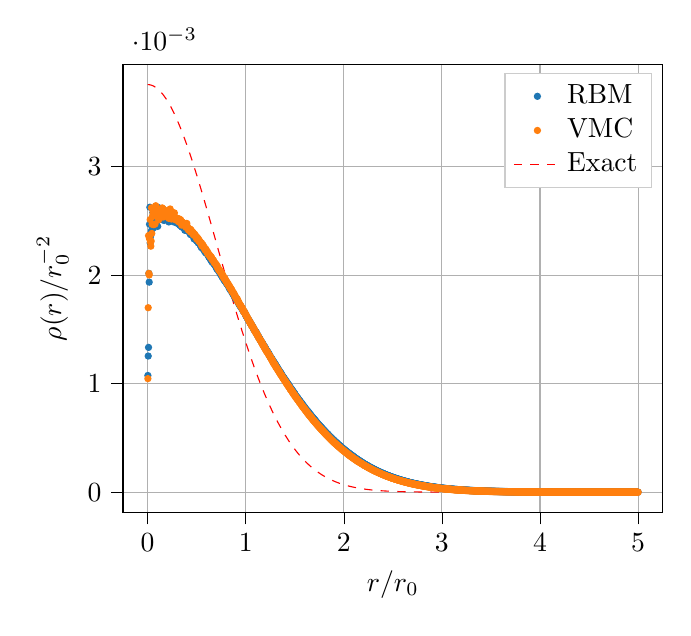
\begin{tikzpicture}

\definecolor{color0}{rgb}{0.12156862745098,0.466666666666667,0.705882352941177}
\definecolor{color1}{rgb}{1,0.498039215686275,0.0549019607843137}

\begin{axis}[
legend cell align={left},
legend style={draw=white!80.0!black},
tick align=outside,
tick pos=left,
x grid style={white!69.01960784313725!black},
xlabel={\(\displaystyle r / r_0\)},
xmajorgrids,
xmin=-0.25, xmax=5.25,
xtick style={color=black},
y grid style={white!69.01960784313725!black},
ylabel={\(\displaystyle \rho(r) / r_0^{-2}\)},
ymajorgrids,
ymin=-0.000187835169088002, ymax=0.00394453855199584,
ytick style={color=black}
]
\addplot [semithick, color0, opacity=1.0, mark=*, mark size=1, mark options={solid}, only marks]
table {%
0 nan
0.00333555703802535 0.00107531090423062
0.0066711140760507 0.00125452938826905
0.0100066711140761 0.00133418204784169
0.0133422281521014 0.00201620794543241
0.0166777851901268 0.00193555962761511
0.0200133422281521 0.00246923244675179
0.0233488992661775 0.00262609941917545
0.0266844563042028 0.00229623682674246
0.0300200133422282 0.00235417860514687
0.0333555703802535 0.00250547440685734
0.0366911274182789 0.00239649179482801
0.0400266844563042 0.00240949295207231
0.0433622414943296 0.00248042623766806
0.0466977985323549 0.00248985679610542
0.0500333555703803 0.0025178205690911
0.0533689126084056 0.00257836592466234
0.056704469646431 0.00250161717858495
0.0600400266844563 0.00243438440818876
0.0633755837224817 0.00248721497238938
0.066711140760507 0.00251577946968955
0.0700466977985324 0.00254766593296362
0.0733822548365577 0.00254164395545419
0.0767178118745831 0.00250092788123201
0.0800533689126084 0.00254328452869822
0.0833889259506338 0.0025850474137704
0.0867244829886591 0.00250667273163227
0.0900600400266845 0.00246972412983557
0.0933955970647098 0.00256483595779497
0.0967311541027352 0.00256617001758722
0.100066711140761 0.00255007989621801
0.103402268178786 0.0024495679374036
0.106737825216811 0.00254773776576906
0.110073382254837 0.00253687137874425
0.113408939292862 0.00256021976246603
0.116744496330887 0.00262083259025677
0.120080053368913 0.00256312855065773
0.123415610406938 0.00253406296240468
0.126751167444963 0.00256900512542354
0.130086724482989 0.00255406959895933
0.133422281521014 0.00256416846037993
0.136757838559039 0.00252217232415067
0.140093395597065 0.00255396499532778
0.14342895263509 0.00252951042614985
0.146764509673115 0.00254747596190791
0.150100066711141 0.00259357909864018
0.153435623749166 0.00255708187693971
0.156771180787191 0.00250865312130036
0.160106737825217 0.00260854681520354
0.163442294863242 0.00255571081840567
0.166777851901268 0.00251809138813364
0.170113408939293 0.00250444222965976
0.173448965977318 0.00254544596135212
0.176784523015344 0.00254612746262794
0.180120080053369 0.00253468775728023
0.183455637091394 0.00256060260500536
0.18679119412942 0.00254471959734167
0.190126751167445 0.00255925539718291
0.19346230820547 0.00255114635156497
0.196797865243496 0.0025231141187221
0.200133422281521 0.00256048452487469
0.203468979319546 0.00254604877808111
0.206804536357572 0.00256579886370636
0.210140093395597 0.0025512331439082
0.213475650433622 0.00254861285602315
0.216811207471648 0.00249056427735686
0.220146764509673 0.00254209652738358
0.223482321547698 0.0025307773898856
0.226817878585724 0.00250235358671573
0.230153435623749 0.00253612411785792
0.233488992661775 0.00253458826671338
0.2368245496998 0.00253298538628972
0.240160106737825 0.0025338810897209
0.243495663775851 0.0025189125982351
0.246831220813876 0.00252630642830733
0.250166777851901 0.00250571336483606
0.253502334889927 0.00252308349170178
0.256837891927952 0.00252867638425289
0.260173448965977 0.00253939984139011
0.263509006004003 0.00249168540963484
0.266844563042028 0.00251667556210974
0.270180120080053 0.00250498873323347
0.273515677118079 0.00249613180378994
0.276851234156104 0.00252505810411593
0.280186791194129 0.0025122337071652
0.283522348232155 0.00250380004731788
0.28685790527018 0.00250115920571651
0.290193462308205 0.00251071623378248
0.293529019346231 0.00248128731723463
0.296864576384256 0.00251360655021463
0.300200133422282 0.00250945703983597
0.303535690460307 0.00249583543470167
0.306871247498332 0.00250698370429853
0.310206804536358 0.00250077025837238
0.313542361574383 0.00248786329036561
0.316877918612408 0.00249994395280695
0.320213475650434 0.0024709242879097
0.323549032688459 0.0024910778807009
0.326884589726484 0.00246296655917295
0.33022014676451 0.0024622107246958
0.333555703802535 0.00245676282289569
0.33689126084056 0.00248838039640741
0.340226817878586 0.00248042929552389
0.343562374916611 0.00245290624180875
0.346897931954636 0.00245625096324017
0.350233488992662 0.00244488149082529
0.353569046030687 0.00244170031640155
0.356904603068712 0.00244494148152357
0.360240160106738 0.0024469684221143
0.363575717144763 0.00244715214759326
0.366911274182789 0.00244365143558656
0.370246831220814 0.00244002453213859
0.373582388258839 0.00246029660450182
0.376917945296865 0.00244672740465192
0.38025350233489 0.0024135610847894
0.383589059372915 0.00245034016093595
0.386924616410941 0.00243576512926823
0.390260173448966 0.00242769104490695
0.393595730486991 0.00242018319249003
0.396931287525017 0.0024104069805435
0.400266844563042 0.00241766979540656
0.403602401601067 0.00241356779955676
0.406937958639093 0.00241993117516398
0.410273515677118 0.00241779701429129
0.413609072715143 0.00241094085258938
0.416944629753169 0.00241491315625091
0.420280186791194 0.00240479687690476
0.423615743829219 0.00241445488459792
0.426951300867245 0.00241179249479557
0.43028685790527 0.00238659658183821
0.433622414943296 0.00239822964182298
0.436957971981321 0.00237426634174502
0.440293529019346 0.00237979806206892
0.443629086057372 0.00238422690691079
0.446964643095397 0.0023804638250817
0.450300200133422 0.00238032631154238
0.453635757171448 0.00236917999001243
0.456971314209473 0.00237364946745669
0.460306871247498 0.00236749273708262
0.463642428285524 0.00236246341802957
0.466977985323549 0.00237074965462151
0.470313542361574 0.00237256029631528
0.4736490993996 0.00233437319404994
0.476984656437625 0.00234615917446356
0.48032021347565 0.00234206130602351
0.483655770513676 0.00233584123484274
0.486991327551701 0.00233247190187779
0.490326884589726 0.00233328217647745
0.493662441627752 0.0023363367989061
0.496997998665777 0.00232196956496769
0.500333555703803 0.00231554264010638
0.503669112741828 0.00232248322478071
0.507004669779853 0.00231427968485679
0.510340226817879 0.00231673328046696
0.513675783855904 0.00230792539944386
0.517011340893929 0.00229750263887608
0.520346897931955 0.00230844689604456
0.52368245496998 0.00229835036372485
0.527018012008005 0.00229678064184284
0.530353569046031 0.00229287794228503
0.533689126084056 0.00228914509532329
0.537024683122081 0.0022766645137589
0.540360240160107 0.00227973642047597
0.543695797198132 0.0022742717023567
0.547031354236157 0.00225600328991081
0.550366911274183 0.00227576864409226
0.553702468312208 0.00226251954463054
0.557038025350234 0.00225296443733986
0.560373582388259 0.00224600307436052
0.563709139426284 0.00225044978586285
0.56704469646431 0.00224741219250524
0.570380253502335 0.00224237926971562
0.57371581054036 0.0022382743316343
0.577051367578386 0.00223465311543812
0.580386924616411 0.00222138339381582
0.583722481654436 0.00222998121620149
0.587058038692462 0.00221788081146184
0.590393595730487 0.00220914855078296
0.593729152768512 0.00220626981521449
0.597064709806538 0.00220531977529785
0.600400266844563 0.00220798831765761
0.603735823882588 0.00220067672525107
0.607071380920614 0.00220639357918543
0.610406937958639 0.00220011306052572
0.613742494996664 0.00218950823874675
0.61707805203469 0.00218985874347657
0.620413609072715 0.00217594323145753
0.62374916611074 0.00217954256414281
0.627084723148766 0.00216471325728261
0.630420280186791 0.00216416817913685
0.633755837224817 0.00216275504876566
0.637091394262842 0.00215398206292472
0.640426951300867 0.00214867230183961
0.643762508338893 0.00215668412664128
0.647098065376918 0.00213685518508587
0.650433622414943 0.00214237375199661
0.653769179452969 0.00212780429478381
0.657104736490994 0.0021264929574447
0.660440293529019 0.00211822405832399
0.663775850567045 0.00212475345021867
0.66711140760507 0.00211592959041349
0.670446964643095 0.00212263957541466
0.673782521681121 0.00211467182091456
0.677118078719146 0.00210267828719064
0.680453635757171 0.00210501187563609
0.683789192795197 0.00210442800431836
0.687124749833222 0.00209335433170656
0.690460306871247 0.00208876593876896
0.693795863909273 0.00209198144094903
0.697131420947298 0.00207456647459478
0.700466977985324 0.00207553292116921
0.703802535023349 0.00207106620773233
0.707138092061374 0.00205585261809862
0.7104736490994 0.00206497663328794
0.713809206137425 0.00205859799301526
0.71714476317545 0.00205243450487501
0.720480320213476 0.00204719550353293
0.723815877251501 0.00204153941191373
0.727151434289526 0.00203325715775329
0.730486991327552 0.00203492441468717
0.733822548365577 0.0020323227975509
0.737158105403602 0.00202714925938547
0.740493662441628 0.00201731342427235
0.743829219479653 0.00200853433532284
0.747164776517678 0.00201187892752236
0.750500333555704 0.00200121465981218
0.753835890593729 0.00200000052555275
0.757171447631754 0.00199844139026756
0.76050700466978 0.00198178740556168
0.763842561707805 0.00199008352185904
0.767178118745831 0.00198579162124154
0.770513675783856 0.00198346743106746
0.773849232821881 0.00197401714929591
0.777184789859907 0.00195758783038716
0.780520346897932 0.00196057938683212
0.783855903935957 0.00195721837206912
0.787191460973983 0.00194540995121714
0.790527018012008 0.00194713804337609
0.793862575050033 0.00194265888675086
0.797198132088059 0.00193980218699112
0.800533689126084 0.00193151476599619
0.803869246164109 0.00193002764816944
0.807204803202135 0.00191896652495557
0.81054036024016 0.00192739465334357
0.813875917278185 0.00191721875185004
0.817211474316211 0.00190953898474306
0.820547031354236 0.00190904882013584
0.823882588392261 0.00190470275731669
0.827218145430287 0.0018973340826536
0.830553702468312 0.00188341424917998
0.833889259506338 0.00188622149583327
0.837224816544363 0.00188110424442673
0.840560373582388 0.00187171896921359
0.843895930620414 0.00186494291387751
0.847231487658439 0.00186791851157197
0.850567044696464 0.00186114640423097
0.85390260173449 0.00186005355890343
0.857238158772515 0.00184678150524435
0.86057371581054 0.00184611408495034
0.863909272848566 0.00184202222505741
0.867244829886591 0.00183126825594197
0.870580386924616 0.00182808852135899
0.873915943962642 0.0018277314236281
0.877251501000667 0.00181769087281037
0.880587058038692 0.00181181514782165
0.883922615076718 0.00180822454379741
0.887258172114743 0.0018012653178743
0.890593729152768 0.0018023186577918
0.893929286190794 0.00179285107082597
0.897264843228819 0.00179536743531795
0.900600400266845 0.00177906427729365
0.90393595730487 0.00177845080043163
0.907271514342895 0.00177055769633301
0.910607071380921 0.00176962412150649
0.913942628418946 0.00176686661296532
0.917278185456971 0.00176442463777906
0.920613742494997 0.00175374189209109
0.923949299533022 0.00175007390385803
0.927284856571047 0.0017445394937013
0.930620413609073 0.00173394188370703
0.933955970647098 0.00173450574868464
0.937291527685123 0.00172538276819405
0.940627084723149 0.00172632445889526
0.943962641761174 0.00171630749946644
0.947298198799199 0.00171091702602186
0.950633755837225 0.00170847232226287
0.95396931287525 0.00170216587348232
0.957304869913275 0.00170076206892511
0.960640426951301 0.00169784578955968
0.963975983989326 0.00168927921378708
0.967311541027352 0.00168691475842224
0.970647098065377 0.00167672065321504
0.973982655103402 0.00167136412260179
0.977318212141428 0.001672661315531
0.980653769179453 0.00166490562962515
0.983989326217478 0.00165812261833398
0.987324883255504 0.00166108673204219
0.990660440293529 0.00164913960272464
0.993995997331554 0.00164833821312875
0.99733155436958 0.00164168509553603
1.00066711140761 0.00162976111961682
1.00400266844563 0.00162397847873577
1.00733822548366 0.00162180702078706
1.01067378252168 0.00161898071386341
1.01400933955971 0.00161181055847016
1.01734489659773 0.00160300602780544
1.02068045363576 0.00160186329314473
1.02401601067378 0.00159190106794841
1.02735156771181 0.00158962699524149
1.03068712474983 0.00158193755732162
1.03402268178786 0.00158360510959565
1.03735823882588 0.00157784382489
1.04069379586391 0.00157333886363509
1.04402935290193 0.00156213818030036
1.04736490993996 0.00155852426117538
1.05070046697799 0.00155566882075357
1.05403602401601 0.00155102527798174
1.05737158105404 0.00154796445476716
1.06070713809206 0.00153450643083996
1.06404269513009 0.00153729413807292
1.06737825216811 0.00153096689917631
1.07071380920614 0.00152625738530752
1.07404936624416 0.00151800565772219
1.07738492328219 0.00151586827631268
1.08072048032021 0.00150445633856092
1.08405603735824 0.00149918107106212
1.08739159439626 0.00149828952836909
1.09072715143429 0.0014936516200094
1.09406270847231 0.00148657854418058
1.09739826551034 0.00148027901168104
1.10073382254837 0.00147806371563336
1.10406937958639 0.00147714694314496
1.10740493662442 0.00147167798549199
1.11074049366244 0.00146731951918361
1.11407605070047 0.00145392433023928
1.11741160773849 0.0014535166013243
1.12074716477652 0.00144970507363928
1.12408272181454 0.00143991334543077
1.12741827885257 0.00144149271366194
1.13075383589059 0.00143209480982908
1.13408939292862 0.0014219885972086
1.13742494996664 0.00141978103419674
1.14076050700467 0.00141591703975427
1.1440960640427 0.00141413801973733
1.14743162108072 0.00140562988306789
1.15076717811875 0.00140118062516389
1.15410273515677 0.00139564545612464
1.1574382921948 0.00138979053116931
1.16077384923282 0.00138590211322896
1.16410940627085 0.00138118343421758
1.16744496330887 0.00137555819080427
1.1707805203469 0.00137321121097146
1.17411607738492 0.00136760840626005
1.17745163442295 0.00136352835328231
1.18078719146097 0.00135275374845233
1.184122748499 0.00135167213490397
1.18745830553702 0.00134300168686914
1.19079386257505 0.00134105132335211
1.19412941961308 0.00134107483937563
1.1974649766511 0.00132839386352261
1.20080053368913 0.00132628730767676
1.20413609072715 0.00132412729082276
1.20747164776518 0.00131187645851034
1.2108072048032 0.00130628647978222
1.21414276184123 0.00130476483144246
1.21747831887925 0.00130096409370751
1.22081387591728 0.0013002865874434
1.2241494329553 0.00129139792063426
1.22748498999333 0.00128583545261816
1.23082054703135 0.00128287428918611
1.23415610406938 0.00127870882873793
1.2374916611074 0.00127456567129797
1.24082721814543 0.00126555182234851
1.24416277518346 0.00126049092859587
1.24749833222148 0.00125316740159133
1.25083388925951 0.00124506665231182
1.25416944629753 0.00124594217395491
1.25750500333556 0.00124121747067311
1.26084056037358 0.00123751489584176
1.26417611741161 0.00123091074245868
1.26751167444963 0.00122745548237699
1.27084723148766 0.00122085516342803
1.27418278852568 0.00121663809780584
1.27751834556371 0.00121033106475076
1.28085390260173 0.00120579536893794
1.28418945963976 0.00120377268230549
1.28752501667779 0.00119755923430846
1.29086057371581 0.00119244449348197
1.29419613075384 0.00118987482968068
1.29753168779186 0.00118335174303976
1.30086724482989 0.00118030159326257
1.30420280186791 0.00117597762461989
1.30753835890594 0.00116883541886357
1.31087391594396 0.00116159857789679
1.31420947298199 0.00115710886366716
1.31754503002001 0.00115561548783001
1.32088058705804 0.00114884584274764
1.32421614409606 0.00114409685259938
1.32755170113409 0.00114114035471982
1.33088725817211 0.00113119925203353
1.33422281521014 0.00113033545929252
1.33755837224817 0.00112166556601532
1.34089392928619 0.00111785649667666
1.34422948632422 0.00111772285932875
1.34756504336224 0.00110958856950993
1.35090060040027 0.00110740251279451
1.35423615743829 0.00110412529103924
1.35757171447632 0.00109805171954495
1.36090727151434 0.00109312573659908
1.36424282855237 0.00108897933889661
1.36757838559039 0.0010827483113969
1.37091394262842 0.00107437089335655
1.37424949966644 0.00107165672397531
1.37758505670447 0.00106712587652535
1.38092061374249 0.00106308528335628
1.38425617078052 0.0010587298775233
1.38759172781855 0.00105402808788519
1.39092728485657 0.00105209141808197
1.3942628418946 0.00104472486009505
1.39759839893262 0.00104006561980007
1.40093395597065 0.00103674235496153
1.40426951300867 0.00103083819551774
1.4076050700467 0.00102963375999791
1.41094062708472 0.00102217006808522
1.41427618412275 0.00101886948317995
1.41761174116077 0.00101392962767383
1.4209472981988 0.00101082124474574
1.42428285523682 0.00100403496933776
1.42761841227485 0.00100283261063218
1.43095396931288 0.000997003057642352
1.4342895263509 0.00099323969439294
1.43762508338893 0.000989516884433125
1.44096064042695 0.000982506682485341
1.44429619746498 0.000979702987107349
1.447631754503 0.000972858476448531
1.45096731154103 0.000965882735601562
1.45430286857905 0.000964966184674042
1.45763842561708 0.000959790064237156
1.4609739826551 0.000954721164587461
1.46430953969313 0.000949505240111731
1.46764509673115 0.000948533266794936
1.47098065376918 0.000945110008557998
1.4743162108072 0.00094019159386131
1.47765176784523 0.000934397427162877
1.48098732488326 0.00093160410970353
1.48432288192128 0.000923292179410922
1.48765843895931 0.000916559885362912
1.49099399599733 0.000919951263764905
1.49432955303536 0.000913339734740981
1.49766511007338 0.000910544505722574
1.50100066711141 0.000906708349654112
1.50433622414943 0.000898874962916127
1.50767178118746 0.00089185810455248
1.51100733822548 0.000888182524378956
1.51434289526351 0.000885163636760137
1.51767845230153 0.00088082259848005
1.52101400933956 0.000876242173453332
1.52434956637759 0.00087421882176394
1.52768512341561 0.000869755255621669
1.53102068045364 0.000865499184162552
1.53435623749166 0.0008617207542222
1.53769179452969 0.000857498898036634
1.54102735156771 0.000852455753827806
1.54436290860574 0.000845930740834129
1.54769846564376 0.000844485195086062
1.55103402268179 0.000839700657999839
1.55436957971981 0.000839183973882291
1.55770513675784 0.000831184280945085
1.56104069379586 0.000827728469645924
1.56437625083389 0.000823614207019668
1.56771180787191 0.00082270695375158
1.57104736490994 0.000816510853098369
1.57438292194797 0.000814024088064949
1.57771847898599 0.000810786828149034
1.58105403602402 0.000803609154254117
1.58438959306204 0.000800332360084756
1.58772515010007 0.000794781328670524
1.59106070713809 0.000791097164706702
1.59439626417612 0.000788938930731183
1.59773182121414 0.000786434056877917
1.60106737825217 0.000779656411343459
1.60440293529019 0.000777341322031401
1.60773849232822 0.000771362144008167
1.61107404936624 0.000767367840790819
1.61440960640427 0.000762973028489565
1.61774516344229 0.000759730182337943
1.62108072048032 0.0007576183778712
1.62441627751835 0.000750966170492457
1.62775183455637 0.000750536101864572
1.6310873915944 0.000746693842495878
1.63442294863242 0.000742416862117074
1.63775850567045 0.000739550466602467
1.64109406270847 0.000736615333711419
1.6444296197465 0.000730376764306553
1.64776517678452 0.000728518481560625
1.65110073382255 0.000722262376402336
1.65443629086057 0.000719198525540478
1.6577718478986 0.000716137498366866
1.66110740493662 0.000710777715401869
1.66444296197465 0.000708833608262719
1.66777851901268 0.000705110034861462
1.6711140760507 0.000699878950647381
1.67444963308873 0.000696931218064326
1.67778519012675 0.000692625050287678
1.68112074716478 0.000689256272938827
1.6844563042028 0.000685884124530857
1.68779186124083 0.000682417027378119
1.69112741827885 0.000679030486552158
1.69446297531688 0.000674872902704055
1.6977985323549 0.000673342302415498
1.70113408939293 0.000666902227824627
1.70446964643095 0.000663376956828543
1.70780520346898 0.000663681438325793
1.711140760507 0.000658591784686583
1.71447631754503 0.000652883421398359
1.71781187458306 0.000650022688038467
1.72114743162108 0.000645192869733814
1.72448298865911 0.000643699095299648
1.72781854569713 0.000638668061623041
1.73115410273516 0.000636007683986462
1.73448965977318 0.000632223690797158
1.73782521681121 0.000627680320497906
1.74116077384923 0.000625350725649948
1.74449633088726 0.000621929660166344
1.74783188792528 0.000618346065536611
1.75116744496331 0.000616243041839947
1.75450300200133 0.000610570731627339
1.75783855903936 0.00060933987735134
1.76117411607738 0.000604636097665027
1.76450967311541 0.000601859809095956
1.76784523015344 0.000598915124466446
1.77118078719146 0.00059681208835031
1.77451634422949 0.000592779142941931
1.77785190126751 0.000589174717970315
1.78118745830554 0.000585067061130751
1.78452301534356 0.000581397973889875
1.78785857238159 0.000579400278821452
1.79119412941961 0.000573879625173662
1.79452968645764 0.000573766140155557
1.79786524349566 0.000568190717178483
1.80120080053369 0.000566580553330332
1.80453635757171 0.000561797938884806
1.80787191460974 0.00056004525605388
1.81120747164777 0.000556884198838397
1.81454302868579 0.000553196328309467
1.81787858572382 0.000548976641968059
1.82121414276184 0.000545628773754542
1.82454969979987 0.000542938404931631
1.82788525683789 0.000540162567742957
1.83122081387592 0.000536890178645886
1.83455637091394 0.00053504567551303
1.83789192795197 0.000534812522681186
1.84122748498999 0.000529653366565585
1.84456304202802 0.000525918100375099
1.84789859906604 0.000521264443347571
1.85123415610407 0.000518054730452175
1.85456971314209 0.000517259621519855
1.85790527018012 0.000512360291784223
1.86124082721815 0.000509795670430758
1.86457638425617 0.000506123125241197
1.8679119412942 0.000505711586095498
1.87124749833222 0.000501113721119454
1.87458305537025 0.000498845132296737
1.87791861240827 0.000495214399996984
1.8812541694463 0.000492902101420471
1.88458972648432 0.000488098011366492
1.88792528352235 0.000485758309221798
1.89126084056037 0.000483986180904423
1.8945963975984 0.000480369797768516
1.89793195463642 0.000478477443477415
1.90126751167445 0.0004749444278159
1.90460306871247 0.00047181908101397
1.9079386257505 0.000467807219284103
1.91127418278853 0.000466621222972157
1.91460973982655 0.000463300745073976
1.91794529686458 0.000461023932094143
1.9212808539026 0.000457845060225266
1.92461641094063 0.000456663720441327
1.92795196797865 0.000451772373546393
1.93128752501668 0.000450805527140737
1.9346230820547 0.000447851754844384
1.93795863909273 0.000444600262339532
1.94129419613075 0.000439636712731549
1.94462975316878 0.00043910213266051
1.9479653102068 0.000434668512103237
1.95130086724483 0.0004331654070186
1.95463642428286 0.000431254067135961
1.95797198132088 0.000428148620016506
1.96130753835891 0.000426382038564835
1.96464309539693 0.000422725447196462
1.96797865243496 0.000420790687756215
1.97131420947298 0.000416214342048488
1.97464976651101 0.000415606122178512
1.97798532354903 0.000411495269729342
1.98132088058706 0.000409488707110687
1.98465643762508 0.00040695770542489
1.98799199466311 0.000405518550198778
1.99132755170113 0.000401262768295446
1.99466310873916 0.000397881131973935
1.99799866577718 0.000397404392397804
2.00133422281521 0.000394741156822714
2.00466977985324 0.000391942098382889
2.00800533689126 0.000389117409655179
2.01134089392929 0.000386927368569912
2.01467645096731 0.000385311192807483
2.01801200800534 0.000381945791447236
2.02134756504336 0.000379328612913439
2.02468312208139 0.000378398395975901
2.02801867911941 0.000374105689363333
2.03135423615744 0.000372526804325137
2.03468979319546 0.000369878341601014
2.03802535023349 0.000368032034629454
2.04136090727151 0.000366015416403907
2.04469646430954 0.000363048480793908
2.04803202134757 0.000360354198355515
2.05136757838559 0.000358666307084803
2.05470313542362 0.000357740792379367
2.05803869246164 0.000354423619710023
2.06137424949967 0.000351963640956005
2.06470980653769 0.00034854948074364
2.06804536357572 0.000347293159009529
2.07138092061374 0.000345353922543202
2.07471647765177 0.000341822092902384
2.07805203468979 0.000339849692051419
2.08138759172782 0.000339001104219082
2.08472314876584 0.000336194835884362
2.08805870580387 0.000335484712622502
2.09139426284189 0.000332489358832834
2.09472981987992 0.000329767209268237
2.09806537691795 0.000328320420723854
2.10140093395597 0.000324522725999082
2.104736490994 0.000323044827255802
2.10807204803202 0.000320235752044415
2.11140760507005 0.000318064961841919
2.11474316210807 0.000315458168033084
2.1180787191461 0.000314816951356639
2.12141427618412 0.000311375811182588
2.12474983322215 0.000310380396096751
2.12808539026017 0.000308329462313382
2.1314209472982 0.00030620249238631
2.13475650433622 0.000304030856799345
2.13809206137425 0.000302522926130695
2.14142761841227 0.000299644953227558
2.1447631754503 0.000296872701591664
2.14809873248833 0.000295283384668918
2.15143428952635 0.000294164293642484
2.15476984656438 0.000291476329061658
2.1581054036024 0.000290774668283025
2.16144096064043 0.000287636311245235
2.16477651767845 0.000285509004253776
2.16811207471648 0.000284144225517204
2.1714476317545 0.000281433251248628
2.17478318879253 0.000281186560271368
2.17811874583055 0.000276821147253466
2.18145430286858 0.000277299327097337
2.1847898599066 0.000274851664404082
2.18812541694463 0.000272579213509827
2.19146097398266 0.000269791185934107
2.19479653102068 0.000268499890396125
2.19813208805871 0.00026704103396971
2.20146764509673 0.000264355492537228
2.20480320213476 0.000262875324980288
2.20813875917278 0.000260723627203615
2.21147431621081 0.000259642130994891
2.21480987324883 0.000257896884647713
2.21814543028686 0.000255907663011948
2.22148098732488 0.000254049219460539
2.22481654436291 0.000252171757826713
2.22815210140093 0.000250187516067363
2.23148765843896 0.000248648072571593
2.23482321547698 0.000247359834937773
2.23815877251501 0.000246227435374459
2.24149432955304 0.000243252866123722
2.24482988659106 0.000242401517831312
2.24816544362909 0.000239702690651563
2.25150100066711 0.000238730231113507
2.25483655770514 0.00023732361900869
2.25817211474316 0.000234912686020153
2.26150767178119 0.000232413176872401
2.26484322881921 0.000231944848844363
2.26817878585724 0.000229647712834303
2.27151434289526 0.000228269661176045
2.27484989993329 0.000227618078552054
2.27818545697131 0.000225392247455459
2.28152101400934 0.000223434336687765
2.28485657104736 0.0002227266857621
2.28819212808539 0.000219942860341359
2.29152768512342 0.000219060382554578
2.29486324216144 0.000217911766252445
2.29819879919947 0.000215796389165869
2.30153435623749 0.000214307438017942
2.30486991327552 0.000211992562146818
2.30820547031354 0.000211043852010747
2.31154102735157 0.000209366062589415
2.31487658438959 0.000208225075086963
2.31821214142762 0.000205844594180905
2.32154769846564 0.000203948634048067
2.32488325550367 0.000203862966968361
2.32821881254169 0.000202092195614035
2.33155436957972 0.000199852409472682
2.33488992661775 0.000199063822253623
2.33822548365577 0.00019709069551505
2.3415610406938 0.000195357108453363
2.34489659773182 0.000194180525265815
2.34823215476985 0.000193459673904957
2.35156771180787 0.000191060011156433
2.3549032688459 0.00019105885006213
2.35823882588392 0.000188026865164281
2.36157438292195 0.000187339848957786
2.36490993995997 0.000186629931549265
2.368245496998 0.000184483049227171
2.37158105403602 0.000182816531190792
2.37491661107405 0.000181344596514384
2.37825216811207 0.000180171741968876
2.3815877251501 0.000179661436297552
2.38492328218813 0.000178153462268161
2.38825883922615 0.000176728367348481
2.39159439626418 0.000175276011361544
2.3949299533022 0.000172994625363108
2.39826551034023 0.000172331052254623
2.40160106737825 0.000172502285177682
2.40493662441628 0.000170650944065946
2.4082721814543 0.000168143590072133
2.41160773849233 0.000167485073075495
2.41494329553035 0.000165731008918728
2.41827885256838 0.000164898735372284
2.4216144096064 0.000163747732561866
2.42494996664443 0.000162278265004869
2.42828552368245 0.000161225081340081
2.43162108072048 0.000160253276037259
2.43495663775851 0.000158552363107376
2.43829219479653 0.000157665083512863
2.44162775183456 0.000156439557306984
2.44496330887258 0.000154767819094643
2.44829886591061 0.000153607242020522
2.45163442294863 0.000152523397780664
2.45496997998666 0.000151734033120347
2.45830553702468 0.000150280899777142
2.46164109406271 0.000149250677951619
2.46497665110073 0.000148440755361984
2.46831220813876 0.000147274654754127
2.47164776517678 0.00014568607086499
2.47498332221481 0.000144819696463735
2.47831887925284 0.000143840908715223
2.48165443629086 0.000142575787030382
2.48498999332889 0.000141614973280009
2.48832555036691 0.000139865297484984
2.49166110740494 0.000139246019673217
2.49499666444296 0.000137651944713935
2.49833222148099 0.000137007015696222
2.50166777851901 0.000135457631479867
2.50500333555704 0.000134630656635107
2.50833889259506 0.000133941021142323
2.51167444963309 0.000132581011726083
2.51501000667111 0.000132035383861891
2.51834556370914 0.000130065725965311
2.52168112074716 0.000129119489823106
2.52501667778519 0.000128368258359199
2.52835223482322 0.000127664519948468
2.53168779186124 0.000126779871324192
2.53502334889927 0.00012553857646817
2.53835890593729 0.000124238685560625
2.54169446297532 0.000123614036015192
2.54503002001334 0.000122725021757103
2.54836557705137 0.000121133734551622
2.55170113408939 0.000120454665535038
2.55503669112742 0.000119808049559116
2.55837224816544 0.000118892956603296
2.56170780520347 0.000118273309453317
2.56504336224149 0.000116647287952608
2.56837891927952 0.000115535618464589
2.57171447631755 0.000114737745265787
2.57505003335557 0.000114102992154092
2.5783855903936 0.000112888668202525
2.58172114743162 0.000111695491910033
2.58505670446965 0.00011114664150917
2.58839226150767 0.000110770782616294
2.5917278185457 0.000108612702319198
2.59506337558372 0.000108369498607324
2.59839893262175 0.000107851641840279
2.60173448965977 0.000107053292295004
2.6050700466978 0.000105561441495343
2.60840560373582 0.000104832397504354
2.61174116077385 0.000104249968184299
2.61507671781187 0.000102987006600004
2.6184122748499 0.000102494446816299
2.62174783188793 0.00010115669615559
2.62508338892595 0.000100464887452599
2.62841894596398 9.94703224478191e-05
2.631754503002 9.87191356608306e-05
2.63509006004003 9.87622783278884e-05
2.63842561707805 9.78974534958238e-05
2.64176117411608 9.63109637210941e-05
2.6450967311541 9.5599683166848e-05
2.64843228819213 9.49439850723833e-05
2.65176784523015 9.4382305003399e-05
2.65510340226818 9.35586809422072e-05
2.6584389593062 9.26026166508839e-05
2.66177451634423 9.13521646008131e-05
2.66511007338225 9.09692398041905e-05
2.66844563042028 9.062070633851e-05
2.67178118745831 8.94420629426627e-05
2.67511674449633 8.90542031509825e-05
2.67845230153436 8.73491694970316e-05
2.68178785857238 8.69476472462406e-05
2.68512341561041 8.61302421041507e-05
2.68845897264843 8.59549986589777e-05
2.69179452968646 8.50458714626915e-05
2.69513008672448 8.44929021605211e-05
2.69846564376251 8.39374763749196e-05
2.70180120080053 8.26836126268838e-05
2.70513675783856 8.24065347955929e-05
2.70847231487658 8.18794147225641e-05
2.71180787191461 8.08096355751316e-05
2.71514342895264 8.00377920034194e-05
2.71847898599066 7.95341804011862e-05
2.72181454302869 7.8469184956029e-05
2.72515010006671 7.80809405192438e-05
2.72848565710474 7.75194590604138e-05
2.73182121414276 7.69302932843961e-05
2.73515677118079 7.66041743635259e-05
2.73849232821881 7.53294021978863e-05
2.74182788525684 7.45271601001649e-05
2.74516344229486 7.45117962114834e-05
2.74849899933289 7.31926181403615e-05
2.75183455637091 7.35640366063635e-05
2.75517011340894 7.2496334928633e-05
2.75850567044696 7.19574022360839e-05
2.76184122748499 7.08138661026804e-05
2.76517678452302 7.0491092938206e-05
2.76851234156104 6.98463002614189e-05
2.77184789859907 6.93126275681385e-05
2.77518345563709 6.85783377498974e-05
2.77851901267512 6.76394556700535e-05
2.78185456971314 6.70936889807644e-05
2.78519012675117 6.6646219089272e-05
2.78852568378919 6.62722411251137e-05
2.79186124082722 6.57325537865309e-05
2.79519679786524 6.51281324620399e-05
2.79853235490327 6.45139288726312e-05
2.80186791194129 6.35113122644713e-05
2.80520346897932 6.3328944000744e-05
2.80853902601734 6.28338037327167e-05
2.81187458305537 6.23905146685479e-05
2.8152101400934 6.19126679090071e-05
2.81854569713142 6.1089024526725e-05
2.82188125416945 6.06091493959661e-05
2.82521681120747 5.98415851473667e-05
2.8285523682455 5.95078818513393e-05
2.83188792528352 5.8822517914555e-05
2.83522348232155 5.82262870779159e-05
2.83855903935957 5.79707395342671e-05
2.8418945963976 5.76957387408557e-05
2.84523015343562 5.68969775510509e-05
2.84856571047365 5.67298959410534e-05
2.85190126751167 5.58833645396879e-05
2.8552368245497 5.5447626286337e-05
2.85857238158773 5.48295351631174e-05
2.86190793862575 5.42984066634129e-05
2.86524349566378 5.41596708687156e-05
2.8685790527018 5.31260676839789e-05
2.87191460973983 5.28286698347451e-05
2.87525016677785 5.25264783511535e-05
2.87858572381588 5.18860069744681e-05
2.8819212808539 5.11753740912651e-05
2.88525683789193 5.10314887631941e-05
2.88859239492995 5.04816398038011e-05
2.89192795196798 5.02870535526459e-05
2.895263509006 4.96936045068722e-05
2.89859906604403 4.91627955396243e-05
2.90193462308205 4.89319263277144e-05
2.90527018012008 4.81328940887025e-05
2.90860573715811 4.7998048593878e-05
2.91194129419613 4.79572859926792e-05
2.91527685123416 4.68272562945183e-05
2.91861240827218 4.64115305126985e-05
2.92194796531021 4.63759262896942e-05
2.92528352234823 4.54716842918166e-05
2.92861907938626 4.51717138358925e-05
2.93195463642428 4.47660583744766e-05
2.93529019346231 4.47645838224465e-05
2.93862575050033 4.39608409880704e-05
2.94196130753836 4.36160882491411e-05
2.94529686457638 4.36104463717718e-05
2.94863242161441 4.31068230051961e-05
2.95196797865243 4.24172722291258e-05
2.95530353569046 4.21629042635253e-05
2.95863909272849 4.1824609071147e-05
2.96197464976651 4.14347742251076e-05
2.96531020680454 4.08293440907181e-05
2.96864576384256 4.02733641230571e-05
2.97198132088059 4.00891025638774e-05
2.97531687791861 3.97287491116645e-05
2.97865243495664 3.93553002541739e-05
2.98198799199466 3.90195241549783e-05
2.98532354903269 3.83555858502259e-05
2.98865910607071 3.8426284596351e-05
2.99199466310874 3.80506477410594e-05
2.99533022014676 3.76303611060808e-05
2.99866577718479 3.72486597700824e-05
3.00200133422282 3.66687656064271e-05
3.00533689126084 3.66841108069771e-05
3.00867244829887 3.63642560987915e-05
3.01200800533689 3.56566997470466e-05
3.01534356237492 3.54320199214822e-05
3.01867911941294 3.51069321964026e-05
3.02201467645097 3.49419232709813e-05
3.02535023348899 3.44263734857635e-05
3.02868579052702 3.41456008888703e-05
3.03202134756504 3.39080579690164e-05
3.03535690460307 3.34392560907847e-05
3.03869246164109 3.3211050588819e-05
3.04202801867912 3.26566768187054e-05
3.04536357571714 3.25561537299877e-05
3.04869913275517 3.2372539517685e-05
3.0520346897932 3.17598122623317e-05
3.05537024683122 3.17597104485983e-05
3.05870580386925 3.13537344469703e-05
3.06204136090727 3.09356277964496e-05
3.0653769179453 3.06266405218988e-05
3.06871247498332 3.06375946490707e-05
3.07204803202135 3.02503727740148e-05
3.07538358905937 2.99859818815021e-05
3.0787191460974 2.96664969217721e-05
3.08205470313542 2.93416068136052e-05
3.08539026017345 2.85662481480157e-05
3.08872581721147 2.87731572937731e-05
3.0920613742495 2.83048450788097e-05
3.09539693128752 2.81504360478077e-05
3.09873248832555 2.7725007549977e-05
3.10206804536358 2.75514488087855e-05
3.1054036024016 2.77340056631061e-05
3.10873915943963 2.72276235127423e-05
3.11207471647765 2.66895827268612e-05
3.11541027351568 2.627992386103e-05
3.1187458305537 2.61862246871614e-05
3.12208138759173 2.59973339251734e-05
3.12541694462975 2.57783660434411e-05
3.12875250166778 2.56276948746549e-05
3.1320880587058 2.52597121616799e-05
3.13542361574383 2.48897884226943e-05
3.13875917278185 2.48322606867451e-05
3.14209472981988 2.44515714037096e-05
3.14543028685791 2.41540635694148e-05
3.14876584389593 2.4103922372633e-05
3.15210140093396 2.37996688117378e-05
3.15543695797198 2.38272812542106e-05
3.15877251501001 2.32152354316929e-05
3.16210807204803 2.31018716973739e-05
3.16544362908606 2.25873544786012e-05
3.16877918612408 2.27628325632774e-05
3.17211474316211 2.24435035622751e-05
3.17545030020013 2.20457734855248e-05
3.17878585723816 2.19841398304466e-05
3.18212141427618 2.17269792382299e-05
3.18545697131421 2.14144497317208e-05
3.18879252835223 2.13479064889055e-05
3.19212808539026 2.08851353929023e-05
3.19546364242829 2.0930603066993e-05
3.19879919946631 2.04707320378149e-05
3.20213475650434 2.05315620060526e-05
3.20547031354236 2.03289492214367e-05
3.20880587058039 1.99997079462241e-05
3.21214142761841 1.97429074396132e-05
3.21547698465644 1.9610941190859e-05
3.21881254169446 1.94571545397577e-05
3.22214809873249 1.93740628730302e-05
3.22548365577051 1.90344496874557e-05
3.22881921280854 1.89127080599565e-05
3.23215476984656 1.86423595383814e-05
3.23549032688459 1.85351798084602e-05
3.23882588392261 1.81020285201305e-05
3.24216144096064 1.81843070129178e-05
3.24549699799867 1.81329399955782e-05
3.24883255503669 1.7829167037108e-05
3.25216811207472 1.76674312107234e-05
3.25550366911274 1.75006762366166e-05
3.25883922615077 1.71875537210986e-05
3.26217478318879 1.70701669357288e-05
3.26551034022682 1.68400949604801e-05
3.26884589726484 1.67626384675184e-05
3.27218145430287 1.66024049920047e-05
3.27551701134089 1.63864769062607e-05
3.27885256837892 1.61038812545784e-05
3.28218812541694 1.60543228563085e-05
3.28552368245497 1.57973088442898e-05
3.288859239493 1.56773497901295e-05
3.29219479653102 1.54897750806936e-05
3.29553035356905 1.53502956669155e-05
3.29886591060707 1.52073174175159e-05
3.3022014676451 1.50798795446197e-05
3.30553702468312 1.48357672094998e-05
3.30887258172115 1.47758215390527e-05
3.31220813875917 1.45864964297116e-05
3.3155436957972 1.44300086846124e-05
3.31887925283522 1.42210801621934e-05
3.32221480987325 1.42741968298504e-05
3.32555036691127 1.39576399442575e-05
3.3288859239493 1.38706632308574e-05
3.33222148098732 1.37439608536281e-05
3.33555703802535 1.34684482939725e-05
3.33889259506338 1.36622657095911e-05
3.3422281521014 1.33599350394747e-05
3.34556370913943 1.29759434959246e-05
3.34889926617745 1.29844219812097e-05
3.35223482321548 1.27921567978842e-05
3.3555703802535 1.27114865506395e-05
3.35890593729153 1.24266283480488e-05
3.36224149432955 1.24998782639202e-05
3.36557705136758 1.23170338211649e-05
3.3689126084056 1.23149680003512e-05
3.37224816544363 1.19495821979036e-05
3.37558372248165 1.19466273168812e-05
3.37891927951968 1.18718804319724e-05
3.3822548365577 1.16567418454793e-05
3.38559039359573 1.15925555658593e-05
3.38892595063376 1.14752984749136e-05
3.39226150767178 1.11770589210707e-05
3.39559706470981 1.12979565871591e-05
3.39893262174783 1.10293236812863e-05
3.40226817878586 1.10047797508607e-05
3.40560373582388 1.09060404890658e-05
3.40893929286191 1.06426010091911e-05
3.41227484989993 1.05868694529632e-05
3.41561040693796 1.03713577556003e-05
3.41894596397598 1.0469174082942e-05
3.42228152101401 1.01901659614512e-05
3.42561707805203 1.01684619843696e-05
3.42895263509006 1.00230234784399e-05
3.43228819212809 9.78960833573225e-06
3.43562374916611 9.76300673770699e-06
3.43895930620414 9.66399055855773e-06
3.44229486324216 9.65200202763189e-06
3.44563042028019 9.38895529163987e-06
3.44896597731821 9.30727331441822e-06
3.45230153435624 9.25918250659125e-06
3.45563709139426 9.19673272367077e-06
3.45897264843229 9.13517312111735e-06
3.46230820547031 9.05902959012377e-06
3.46564376250834 8.95294710082044e-06
3.46897931954636 8.84659288351711e-06
3.47231487658439 8.77982551979461e-06
3.47565043362241 8.67335301436009e-06
3.47898599066044 8.55343386149325e-06
3.48232154769847 8.39202831163451e-06
3.48565710473649 8.31508776107819e-06
3.48899266177452 8.26119444738445e-06
3.49232821881254 8.29070783406553e-06
3.49566377585057 8.053135219634e-06
3.49899933288859 8.07834237408951e-06
3.50233488992662 7.90788353108191e-06
3.50567044696464 7.84822439044255e-06
3.50900600400267 7.83897876654334e-06
3.51234156104069 7.70562108356661e-06
3.51567711807872 7.52113116055213e-06
3.51901267511674 7.50816800361918e-06
3.52234823215477 7.3919010370608e-06
3.5256837891928 7.29498885084342e-06
3.52901934623082 7.27720253332696e-06
3.53235490326885 7.16646373563499e-06
3.53569046030687 7.11211550800092e-06
3.5390260173449 7.13549134697026e-06
3.54236157438292 6.8854523603171e-06
3.54569713142095 6.80731713430163e-06
3.54903268845897 6.78692871249067e-06
3.552368245497 6.69107621952577e-06
3.55570380253502 6.57033715230196e-06
3.55903935957305 6.56007382182327e-06
3.56237491661107 6.40135597550983e-06
3.5657104736491 6.3624105818761e-06
3.56904603068712 6.29057035511276e-06
3.57238158772515 6.22883060385487e-06
3.57571714476318 6.21331625098795e-06
3.5790527018012 6.2243114720127e-06
3.58238825883923 5.99256309700284e-06
3.58572381587725 6.02809949124847e-06
3.58905937291528 5.9381091560012e-06
3.5923949299533 5.86404782078107e-06
3.59573048699133 5.68152470215233e-06
3.59906604402935 5.48796870618221e-06
3.60240160106738 5.61778653413349e-06
3.6057371581054 5.54405716047808e-06
3.60907271514343 5.42833959498818e-06
3.61240827218145 5.43405808039713e-06
3.61574382921948 5.4235792101881e-06
3.6190793862575 5.34370915350349e-06
3.62241494329553 5.24908011739882e-06
3.62575050033356 5.20241711151386e-06
3.62908605737158 5.15394851727776e-06
3.63242161440961 5.03658644718577e-06
3.63575717144763 5.0087953560275e-06
3.63909272848566 5.07279368967408e-06
3.64242828552368 4.84032264029931e-06
3.64576384256171 4.78946478958348e-06
3.64909939959973 4.73474164113656e-06
3.65243495663776 4.76271785442399e-06
3.65577051367578 4.65332238221501e-06
3.65910607071381 4.66062864577451e-06
3.66244162775183 4.5934246707772e-06
3.66577718478986 4.57379200050402e-06
3.66911274182789 4.49008954018611e-06
3.67244829886591 4.41259731233613e-06
3.67578385590394 4.36976435550121e-06
3.67911941294196 4.33709647640256e-06
3.68245496997999 4.28027762342703e-06
3.68579052701801 4.24244471869696e-06
3.68912608405604 4.1550740881809e-06
3.69246164109406 4.19627088725426e-06
3.69579719813209 4.11614609204778e-06
3.69913275517011 3.99171296512824e-06
3.70246831220814 3.91543150178283e-06
3.70580386924616 3.94758911501708e-06
3.70913942628419 3.97339256824968e-06
3.71247498332221 3.88436994948047e-06
3.71581054036024 3.80446975131956e-06
3.71914609739827 3.7993785238529e-06
3.72248165443629 3.78580945177286e-06
3.72581721147432 3.671160052749e-06
3.72915276851234 3.64624253082382e-06
3.73248832555037 3.52622848919185e-06
3.73582388258839 3.54822309557921e-06
3.73915943962642 3.55273435761008e-06
3.74249499666444 3.42425687877239e-06
3.74583055370247 3.42256658088244e-06
3.74916611074049 3.37704312177769e-06
3.75250166777852 3.3356409758099e-06
3.75583722481654 3.22964069302534e-06
3.75917278185457 3.19696124791958e-06
3.76250833889259 3.21031047875801e-06
3.76584389593062 3.19197171959836e-06
3.76917945296865 3.16569262079014e-06
3.77251501000667 3.14776770155715e-06
3.7758505670447 3.06123045817254e-06
3.77918612408272 3.03139696914639e-06
3.78252168112075 2.96877354045299e-06
3.78585723815877 2.9852473213117e-06
3.7891927951968 2.96207895728139e-06
3.79252835223482 2.94716670354341e-06
3.79586390927285 2.84705529088027e-06
3.79919946631087 2.82603343966088e-06
3.8025350233489 2.82673167576167e-06
3.80587058038692 2.77139502048328e-06
3.80920613742495 2.73479949672658e-06
3.81254169446298 2.69764184336001e-06
3.815877251501 2.67389306883474e-06
3.81921280853903 2.66238950068274e-06
3.82254836557705 2.61544172543445e-06
3.82588392261508 2.57968775847221e-06
3.8292194796531 2.54962983437082e-06
3.83255503669113 2.49075765367336e-06
3.83589059372915 2.49875964248372e-06
3.83922615076718 2.4531593722778e-06
3.8425617078052 2.4147359310885e-06
3.84589726484323 2.41324534644496e-06
3.84923282188125 2.35590680113242e-06
3.85256837891928 2.30292779624585e-06
3.8559039359573 2.29103261666872e-06
3.85923949299533 2.27368601808597e-06
3.86257505003336 2.19170978471183e-06
3.86591060707138 2.23355845968748e-06
3.86924616410941 2.22478118116679e-06
3.87258172114743 2.13771785317535e-06
3.87591727818546 2.1688154357198e-06
3.87925283522348 2.11566399543514e-06
3.88258839226151 2.09959657209269e-06
3.88592394929953 2.00369229626571e-06
3.88925950633756 2.00658432902586e-06
3.89259506337558 2.01985955647337e-06
3.89593062041361 1.99853601584251e-06
3.89926617745163 1.95472540530053e-06
3.90260173448966 1.91721490266554e-06
3.90593729152768 1.93302372006706e-06
3.90927284856571 1.91224279117063e-06
3.91260840560374 1.83187414431745e-06
3.91594396264176 1.8768661709344e-06
3.91927951967979 1.8492686454407e-06
3.92261507671781 1.83718332654573e-06
3.92595063375584 1.75359539224329e-06
3.92928619079386 1.77489949162794e-06
3.93262174783189 1.73978625350954e-06
3.93595730486991 1.70659141041771e-06
3.93929286190794 1.70884231723368e-06
3.94262841894596 1.73725161784676e-06
3.94596397598399 1.69641008829449e-06
3.94929953302201 1.63256428703863e-06
3.95263509006004 1.63338365199587e-06
3.95597064709807 1.54959576372708e-06
3.95930620413609 1.58336463705763e-06
3.96264176117412 1.54108107044807e-06
3.96597731821214 1.54723711233625e-06
3.96931287525017 1.50110192725082e-06
3.97264843228819 1.44160048874716e-06
3.97598398932622 1.5113310462849e-06
3.97931954636424 1.48613246777031e-06
3.98265510340227 1.48603268984394e-06
3.98599066044029 1.43158925608896e-06
3.98932621747832 1.39699646608299e-06
3.99266177451634 1.39728999831336e-06
3.99599733155437 1.34875519166554e-06
3.99933288859239 1.34775297940078e-06
4.00266844563042 1.33891142450382e-06
4.00600400266845 1.30065015963962e-06
4.00933955970647 1.32106282582921e-06
4.0126751167445 1.27998253950969e-06
4.01601067378252 1.2687084601732e-06
4.01934623082055 1.2575934531896e-06
4.02268178785857 1.2578499741923e-06
4.0260173448966 1.23263921660044e-06
4.02935290193462 1.21131742307841e-06
4.03268845897265 1.2151997565166e-06
4.03602401601067 1.214416078236e-06
4.0393595730487 1.17623812333403e-06
4.04269513008672 1.13550035327809e-06
4.04603068712475 1.14264239545931e-06
4.04936624416278 1.15073220069516e-06
4.0527018012008 1.11642410826091e-06
4.05603735823883 1.10186225761328e-06
4.05937291527685 1.09920518551225e-06
4.06270847231488 1.04726653436628e-06
4.0660440293529 1.08462592689691e-06
4.06937958639093 1.03360082436572e-06
4.07271514342895 9.84905190913657e-07
4.07605070046698 9.7453270134288e-07
4.079386257505 1.01271996938808e-06
4.08272181454303 9.8379149895079e-07
4.08605737158105 9.70720758526886e-07
4.08939292861908 9.73668757040808e-07
4.0927284856571 9.7529641722405e-07
4.09606404269513 9.15236199840314e-07
4.09939959973316 9.04967077668808e-07
4.10273515677118 9.07760752982045e-07
4.10607071380921 9.0593171378597e-07
4.10940627084723 8.62072382545422e-07
4.11274182788526 8.97218806435183e-07
4.11607738492328 8.54101733085886e-07
4.11941294196131 8.159406993479e-07
4.12274849899933 8.71400396045747e-07
4.12608405603736 8.06159859228984e-07
4.12941961307538 8.03337882341924e-07
4.13275517011341 8.16518096856744e-07
4.13609072715143 8.18115595386175e-07
4.13942628418946 7.74788252519126e-07
4.14276184122749 7.67034905275733e-07
4.14609739826551 8.12547356549368e-07
4.14943295530354 7.4314588615363e-07
4.15276851234156 7.41490065088299e-07
4.15610406937959 7.40531224867613e-07
4.15943962641761 7.32774615141376e-07
4.16277518345564 6.87990089313292e-07
4.16611074049366 7.26179045787121e-07
4.16944629753169 6.9106647445221e-07
4.17278185456971 6.66486204867408e-07
4.17611741160774 6.57304265084472e-07
4.17945296864576 6.68241395788817e-07
4.18278852568379 6.50422563845045e-07
4.18612408272181 6.3971449168368e-07
4.18945963975984 6.54146739658122e-07
4.19279519679787 6.24296168123617e-07
4.19613075383589 6.38478957570564e-07
4.19946631087392 6.20505223646576e-07
4.20280186791194 5.87460941632667e-07
4.20613742494997 5.9419367950655e-07
4.20947298198799 5.88076053144876e-07
4.21280853902602 5.68832007571989e-07
4.21614409606404 5.81280909689438e-07
4.21947965310207 5.56171158265165e-07
4.22281521014009 5.8458944128298e-07
4.22615076717812 5.53746821183378e-07
4.22948632421614 5.30468985124564e-07
4.23282188125417 5.26851000140935e-07
4.23615743829219 5.21910359928411e-07
4.23949299533022 5.27967759601816e-07
4.24282855236825 5.18055091921654e-07
4.24616410940627 5.38696460076446e-07
4.2494996664443 5.020753476256e-07
4.25283522348232 4.94563087671772e-07
4.25617078052035 4.86743531668545e-07
4.25950633755837 4.96861689672392e-07
4.2628418945964 4.90488257799507e-07
4.26617745163442 4.69234337039249e-07
4.26951300867245 4.63688448388019e-07
4.27284856571047 4.605620408956e-07
4.2761841227485 4.53410145901014e-07
4.27951967978652 4.32670563723313e-07
4.28285523682455 4.46346051245268e-07
4.28619079386258 4.41310152220492e-07
4.2895263509006 4.43441655854338e-07
4.29286190793863 4.32473851358984e-07
4.29619746497665 4.36988088769406e-07
4.29953302201468 3.95429827540493e-07
4.3028685790527 4.13771657758351e-07
4.30620413609073 4.03130591072975e-07
4.30953969312875 3.98426967973093e-07
4.31287525016678 3.93951803566741e-07
4.3162108072048 3.8413838403734e-07
4.31954636424283 3.7959127341842e-07
4.32288192128085 3.98105378817185e-07
4.32621747831888 3.78421501314358e-07
4.3295530353569 3.70179750554817e-07
4.33288859239493 3.63131227803832e-07
4.33622414943296 3.61088129083358e-07
4.33955970647098 3.54392007376012e-07
4.34289526350901 3.48667511614391e-07
4.34623082054703 3.39476728340827e-07
4.34956637758506 3.04807679908421e-07
4.35290193462308 3.366479825246e-07
4.35623749166111 3.33821005062107e-07
4.35957304869913 3.18097914065536e-07
4.36290860573716 3.18449737370619e-07
4.36624416277518 3.13884233673643e-07
4.36957971981321 3.29592410480336e-07
4.37291527685123 3.09799040145663e-07
4.37625083388926 2.92980841763273e-07
4.37958639092728 3.08024313781678e-07
4.38292194796531 2.88249092535102e-07
4.38625750500334 3.00558691732692e-07
4.38959306204136 2.76507855936464e-07
4.39292861907939 2.72988318074977e-07
4.39626417611741 2.71852041328817e-07
4.39959973315544 2.81535289546694e-07
4.40293529019346 2.7246887294411e-07
4.40627084723149 2.52851312778685e-07
4.40960640426951 2.53904576845224e-07
4.41294196130754 2.65398282624367e-07
4.41627751834556 2.56102937242884e-07
4.41961307538359 2.45916598390085e-07
4.42294863242161 2.32498971772164e-07
4.42628418945964 2.41206662603145e-07
4.42961974649767 2.4541651486565e-07
4.43295530353569 2.43423826764416e-07
4.43629086057372 2.35560503922983e-07
4.43962641761174 2.35004348380489e-07
4.44296197464977 2.22934192228731e-07
4.44629753168779 2.33997105598139e-07
4.44963308872582 2.26898869458784e-07
4.45296864576384 2.06748981291938e-07
4.45630420280187 2.1407062818783e-07
4.45963975983989 2.14552588371276e-07
4.46297531687792 2.00016607294199e-07
4.46631087391594 2.19209957101451e-07
4.46964643095397 1.94429498166002e-07
4.47298198799199 1.98823696439366e-07
4.47631754503002 2.05990937053468e-07
4.47965310206805 1.96045942978836e-07
4.48298865910607 1.94365284327665e-07
4.4863242161441 1.94373580068496e-07
4.48965977318212 1.81818548637118e-07
4.49299533022015 1.88166621799837e-07
4.49633088725817 1.72600108231154e-07
4.4996664442962 1.73723064139321e-07
4.50300200133422 1.79562662197083e-07
4.50633755837225 1.68495918318013e-07
4.50967311541027 1.83639961728839e-07
4.5130086724483 1.71718384976484e-07
4.51634422948632 1.78210028386852e-07
4.51967978652435 1.68478699064741e-07
4.52301534356238 1.6072523743451e-07
4.5263509006004 1.64089455688864e-07
4.52968645763843 1.56656455862905e-07
4.53302201467645 1.56911186313656e-07
4.53635757171448 1.53289166170418e-07
4.5396931287525 1.61191280781266e-07
4.54302868579053 1.61147892651663e-07
4.54636424282855 1.44994012447064e-07
4.54969979986658 1.39772415710526e-07
4.5530353569046 1.43126624132455e-07
4.55637091394263 1.46086678476053e-07
4.55970647098065 1.44530339422945e-07
4.56304202801868 1.2181414350617e-07
4.5663775850567 1.50993423882308e-07
4.56971314209473 1.30338979547374e-07
4.57304869913276 1.31293078051036e-07
4.57638425617078 1.17772603653423e-07
4.57971981320881 1.18646876728313e-07
4.58305537024683 1.32334203490897e-07
4.58639092728486 1.19060319181369e-07
4.58972648432288 1.2238958340113e-07
4.59306204136091 1.32230802424187e-07
4.59639759839893 1.09953811767743e-07
4.59973315543696 1.0988864480142e-07
4.60306871247498 1.10670519444025e-07
4.60640426951301 1.02898622623936e-07
4.60973982655103 1.10256595940552e-07
4.61307538358906 1.0016503437678e-07
4.61641094062708 1.09189650335406e-07
4.61974649766511 1.05014571314211e-07
4.62308205470314 1.04116733291946e-07
4.62641761174116 8.74773200483486e-08
4.62975316877919 9.44212856280535e-08
4.63308872581721 1.02924334682817e-07
4.63642428285524 9.88804430334729e-08
4.63975983989326 9.75341965177565e-08
4.64309539693129 9.11046532205065e-08
4.64643095396931 8.69100880673331e-08
4.64976651100734 8.88144312523101e-08
4.65310206804536 8.43586959978456e-08
4.65643762508339 9.43537843610867e-08
4.65977318212141 8.68722607347889e-08
4.66310873915944 9.34421108609921e-08
4.66644429619747 8.81807234561059e-08
4.66977985323549 8.15626978379005e-08
4.67311541027352 8.49159900345199e-08
4.67645096731154 8.8441990104458e-08
4.67978652434957 7.86649371188655e-08
4.68312208138759 8.25532988302145e-08
4.68645763842562 8.17095202110371e-08
4.68979319546364 8.98433242221865e-08
4.69312875250167 7.36012432119273e-08
4.69646430953969 7.63895934617116e-08
4.69979986657772 7.29410774107325e-08
4.70313542361574 8.01394458579396e-08
4.70647098065377 7.29144813235348e-08
4.70980653769179 7.67664180400415e-08
4.71314209472982 7.07334259032809e-08
4.71647765176785 6.77650520122366e-08
4.71981320880587 7.44720392163612e-08
4.7231487658439 7.01658756514393e-08
4.72648432288192 6.78354470138596e-08
4.72981987991995 6.07875601595313e-08
4.73315543695797 6.4173137536788e-08
4.736490993996 6.59492735352706e-08
4.73982655103402 6.15074720841327e-08
4.74316210807205 5.83189236932249e-08
4.74649766511007 5.96530832646014e-08
4.7498332221481 6.29278384966419e-08
4.75316877918612 5.4984605998619e-08
4.75650433622415 5.45549795619874e-08
4.75983989326217 4.65575936188763e-08
4.7631754503002 6.56518526904447e-08
4.76651100733823 5.60814456225711e-08
4.76984656437625 5.04816112309351e-08
4.77318212141428 5.08486777638266e-08
4.7765176784523 5.06902878061961e-08
4.77985323549033 4.75649364573892e-08
4.78318879252835 5.82184929738213e-08
4.78652434956638 5.53523562740572e-08
4.7898599066044 5.21465006590681e-08
4.79319546364243 4.49571759827435e-08
4.79653102068045 5.00948252257985e-08
4.79986657771848 5.04579690814978e-08
4.8032021347565 4.76221955561238e-08
4.80653769179453 4.07377310296323e-08
4.80987324883256 4.36116778608501e-08
4.81320880587058 4.94900601811315e-08
4.81654436290861 3.76463194769238e-08
4.81987991994663 4.47182529826153e-08
4.82321547698466 3.73708264898055e-08
4.82655103402268 4.54506667152589e-08
4.82988659106071 4.27381461661818e-08
4.83322214809873 4.55813606854469e-08
4.83655770513676 4.04040720257878e-08
4.83989326217478 4.29872192705381e-08
4.84322881921281 3.86777287513985e-08
4.84656437625083 3.71813951194955e-08
4.84989993328886 3.39089215612457e-08
4.85323549032688 3.90263323020366e-08
4.85657104736491 3.92263618306564e-08
4.85990660440294 3.79906049922987e-08
4.86324216144096 3.79385095510585e-08
4.86657771847899 3.78865211919007e-08
4.86991327551701 3.30422519361538e-08
4.87324883255504 3.70272072567805e-08
4.87658438959306 3.17780514720233e-08
4.87991994663109 3.83494928629614e-08
4.88325550366911 3.01861584857507e-08
4.88659106070714 2.7556337165341e-08
4.88992661774516 3.24387761013866e-08
4.89326217478319 3.31440552167209e-08
4.89659773182121 3.11861638266737e-08
4.89993328885924 3.18081185835708e-08
4.90326884589726 3.06866764284425e-08
4.90660440293529 2.94026048280095e-08
4.90993995997332 2.56406407154175e-08
4.91327551701134 2.2714856606779e-08
4.91661107404937 2.53236444825643e-08
4.91994663108739 2.25709231262426e-08
4.92328218812542 2.49260070172655e-08
4.92661774516344 2.53030297024877e-08
4.92995330220147 2.428430296371e-08
4.93328885923949 2.07284568871683e-08
4.93662441627752 2.59369336377759e-08
4.93995997331554 2.42677287320307e-08
4.94329553035357 3.09261317777192e-08
4.94663108739159 2.28169992805685e-08
4.94996664442962 2.42510899021067e-08
4.95330220146765 2.02362128696938e-08
4.95663775850567 1.96408621052214e-08
4.9599733155437 1.95334027626396e-08
4.96330887258172 2.17735486970763e-08
4.96664442961975 2.06934722614777e-08
4.96997998665777 2.08271559307763e-08
4.9733155436958 2.01542908286333e-08
4.97665110073382 2.01272834067704e-08
4.97998665777185 2.06631394814013e-08
4.98332221480987 1.87084378482048e-08
4.9866577718479 1.74806230446546e-08
4.98999332888592 2.3222961931973e-08
4.99332888592395 2.13525850356971e-08
4.99666444296197 1.89281216598141e-08
5 1.88231167823561e-08
};
\addlegendentry{RBM}
\addplot [semithick, color1, opacity=1.0, mark=*, mark size=1, mark options={solid}, only marks]
table {%
0 nan
0.00333555703802535 0.00104624946176196
0.0066711140760507 0.00170015537536318
0.0100066711140761 0.00236374878398072
0.0133422281521014 0.00201620990027044
0.0166777851901268 0.00200182397017121
0.0200133422281521 0.00233468629893178
0.0233488992661775 0.00237007531133832
0.0266844563042028 0.00251208855141804
0.0300200133422282 0.00230131826054225
0.0333555703802535 0.00226687383381758
0.0366911274182789 0.00231443062753403
0.0400266844563042 0.00262046740191305
0.0433622414943296 0.00238449951295058
0.0466977985323549 0.00246882844931075
0.0500333555703803 0.00254199869228091
0.0533689126084056 0.00254750845507144
0.056704469646431 0.00257761113070766
0.0600400266844563 0.00255050216012856
0.0633755837224817 0.0024654003937364
0.066711140760507 0.00255590024762932
0.0700466977985324 0.00254800889327062
0.0733822548365577 0.00256338323706485
0.0767178118745831 0.00247124518425627
0.0800533689126084 0.00259140491686411
0.0833889259506338 0.00263989664191778
0.0867244829886591 0.00256480729741104
0.0900600400266845 0.00261777643107519
0.0933955970647098 0.00254934339513511
0.0967311541027352 0.00260131703275179
0.100066711140761 0.00259547366477096
0.103402268178786 0.00258913173254967
0.106737825216811 0.0025630046629198
0.110073382254837 0.00252931688062319
0.113408939292862 0.00250958078075746
0.116744496330887 0.00260822161739651
0.120080053368913 0.00257202992683148
0.123415610406938 0.00258670977227439
0.126751167444963 0.00254667069472506
0.130086724482989 0.00258707707145741
0.133422281521014 0.00258859554330938
0.136757838559039 0.00255753326192158
0.140093395597065 0.00253654206243498
0.14342895263509 0.00257582581116859
0.146764509673115 0.00257950571069221
0.150100066711141 0.00261992920774548
0.153435623749166 0.00257969385247293
0.156771180787191 0.00260962433653151
0.160106737825217 0.00253592887118475
0.163442294863242 0.00259114870864523
0.166777851901268 0.00257760992396088
0.170113408939293 0.00255166607485082
0.173448965977318 0.0025623567624291
0.176784523015344 0.00256260970873356
0.180120080053369 0.00254631620549188
0.183455637091394 0.00257659826125818
0.18679119412942 0.00257564420271448
0.190126751167445 0.00259351147741475
0.19346230820547 0.00257503639080206
0.196797865243496 0.00258687007827489
0.200133422281521 0.0025775033615157
0.203468979319546 0.00255859213980469
0.206804536357572 0.00256000876366087
0.210140093395597 0.00257023960745772
0.213475650433622 0.0025555545629927
0.216811207471648 0.00252296763698259
0.220146764509673 0.00254200669847514
0.223482321547698 0.00256955356226672
0.226817878585724 0.00258752908083899
0.230153435623749 0.00261023967796861
0.233488992661775 0.00252889882657109
0.2368245496998 0.00257691595263568
0.240160106737825 0.00252762890800671
0.243495663775851 0.00251755617342346
0.246831220813876 0.00256247688207471
0.250166777851901 0.00253573669550236
0.253502334889927 0.0025247228831282
0.256837891927952 0.00253227427073611
0.260173448965977 0.0025773895764411
0.263509006004003 0.00254563340439919
0.266844563042028 0.00255581850939012
0.270180120080053 0.00254949885989025
0.273515677118079 0.00257371558554194
0.276851234156104 0.00252333581539623
0.280186791194129 0.0025202067710937
0.283522348232155 0.00251000917586579
0.28685790527018 0.00251179089278601
0.290193462308205 0.00251690566119465
0.293529019346231 0.00252397774984715
0.296864576384256 0.00251686770849184
0.300200133422282 0.00251013759756058
0.303535690460307 0.00251817080030043
0.306871247498332 0.00251273751286348
0.310206804536358 0.00250925274138497
0.313542361574383 0.00249749234917427
0.316877918612408 0.00252081393863637
0.320213475650434 0.0024901403205217
0.323549032688459 0.00251534279144401
0.326884589726484 0.0025131665928902
0.33022014676451 0.0025040350984043
0.333555703802535 0.00249812983984903
0.33689126084056 0.0025102397389103
0.340226817878586 0.0024987535804451
0.343562374916611 0.00249021310057884
0.346897931954636 0.0024613689260682
0.350233488992662 0.00249133902446498
0.353569046030687 0.00248893956818853
0.356904603068712 0.00248346791184065
0.360240160106738 0.00247035607867415
0.363575717144763 0.00246841547746311
0.366911274182789 0.0024650703744183
0.370246831220814 0.00247003525231165
0.373582388258839 0.00247698837216967
0.376917945296865 0.00245957524811422
0.38025350233489 0.00245692048120134
0.383589059372915 0.00247516120303565
0.386924616410941 0.00246857905667138
0.390260173448966 0.0024452358393645
0.393595730486991 0.00244009659733251
0.396931287525017 0.00244425329732864
0.400266844563042 0.00247699560072144
0.403602401601067 0.00245300395457909
0.406937958639093 0.00243499261658525
0.410273515677118 0.00243439085055418
0.413609072715143 0.00243272052269209
0.416944629753169 0.00241445359789587
0.420280186791194 0.0024229611259682
0.423615743829219 0.00242494535489164
0.426951300867245 0.00241682305935025
0.43028685790527 0.00241918074572902
0.433622414943296 0.00242502878204132
0.436957971981321 0.00239830786823565
0.440293529019346 0.0024150684889845
0.443629086057372 0.00241565785332474
0.446964643095397 0.0024023358311269
0.450300200133422 0.00240471851599046
0.453635757171448 0.00239337483653818
0.456971314209473 0.00239287269009136
0.460306871247498 0.00238160380787658
0.463642428285524 0.0023939118358513
0.466977985323549 0.00237251300141079
0.470313542361574 0.00238241332847571
0.4736490993996 0.00237733260832566
0.476984656437625 0.00236625960228902
0.48032021347565 0.00237709431747976
0.483655770513676 0.00236956634935889
0.486991327551701 0.00236435232091925
0.490326884589726 0.00235833411579584
0.493662441627752 0.00235746854159432
0.496997998665777 0.0023478209904991
0.500333555703803 0.00233490329882014
0.503669112741828 0.00235034833694706
0.507004669779853 0.00234387231177879
0.510340226817879 0.00234012783304129
0.513675783855904 0.00232629776808109
0.517011340893929 0.00233514315353546
0.520346897931955 0.00232774311648296
0.52368245496998 0.00231282154132528
0.527018012008005 0.00231934556615719
0.530353569046031 0.00231096935225068
0.533689126084056 0.00230903033068506
0.537024683122081 0.00230785573858626
0.540360240160107 0.00229731834833387
0.543695797198132 0.00229714939786533
0.547031354236157 0.00228493631523036
0.550366911274183 0.0022962405542472
0.553702468312208 0.00227022135622814
0.557038025350234 0.0022777406126225
0.560373582388259 0.0022824553787354
0.563709139426284 0.00226805827177833
0.56704469646431 0.00227495903727064
0.570380253502335 0.00225872787001808
0.57371581054036 0.00225865138249728
0.577051367578386 0.00225485420603396
0.580386924616411 0.00224786169288485
0.583722481654436 0.00224028343933361
0.587058038692462 0.00223129067885999
0.590393595730487 0.00224448767756615
0.593729152768512 0.00223528337853776
0.597064709806538 0.00223300131293284
0.600400266844563 0.00222498618175537
0.603735823882588 0.00221502070430136
0.607071380920614 0.00221333583002315
0.610406937958639 0.00221679877895496
0.613742494996664 0.00219648726942506
0.61707805203469 0.00219946755001378
0.620413609072715 0.00219518032231287
0.62374916611074 0.00218836548105761
0.627084723148766 0.00218984476312906
0.630420280186791 0.0021857468599319
0.633755837224817 0.0021801597510034
0.637091394262842 0.00217009554350986
0.640426951300867 0.00217221262763277
0.643762508338893 0.00216417946867725
0.647098065376918 0.00216973427676537
0.650433622414943 0.0021592956347228
0.653769179452969 0.00215950998143378
0.657104736490994 0.00214814217351945
0.660440293529019 0.00214456587332235
0.663775850567045 0.00213909900118958
0.66711140760507 0.00213546926079303
0.670446964643095 0.00213931570162236
0.673782521681121 0.00212536622660863
0.677118078719146 0.00212624071620711
0.680453635757171 0.00211535169074666
0.683789192795197 0.00211127041892353
0.687124749833222 0.0021091367784532
0.690460306871247 0.00210749510883588
0.693795863909273 0.00210310313000003
0.697131420947298 0.00209942904976347
0.700466977985324 0.00209078285297817
0.703802535023349 0.00209337234516754
0.707138092061374 0.00207963341972956
0.7104736490994 0.00207413861259635
0.713809206137425 0.00207821263949427
0.71714476317545 0.00206336916565939
0.720480320213476 0.0020593663450827
0.723815877251501 0.00205082432350173
0.727151434289526 0.0020497601188126
0.730486991327552 0.00205025860935633
0.733822548365577 0.00204154830407406
0.737158105403602 0.00203405025014668
0.740493662441628 0.00203062349881782
0.743829219479653 0.00203561642448344
0.747164776517678 0.00202606922784743
0.750500333555704 0.00202145729340428
0.753835890593729 0.00201349489425174
0.757171447631754 0.0020152858526673
0.76050700466978 0.00200242333360941
0.763842561707805 0.00199654134908303
0.767178118745831 0.00200014944362246
0.770513675783856 0.00198545447277357
0.773849232821881 0.001982069687639
0.777184789859907 0.0019798774444098
0.780520346897932 0.00196992122113307
0.783855903935957 0.00196898875618944
0.787191460973983 0.0019723907526751
0.790527018012008 0.00196002813363731
0.793862575050033 0.00195365839621027
0.797198132088059 0.00195221688622197
0.800533689126084 0.00194486452681748
0.803869246164109 0.00193975537682017
0.807204803202135 0.00193229100700079
0.81054036024016 0.00193520743303498
0.813875917278185 0.00191882109111003
0.817211474316211 0.00191803976712616
0.820547031354236 0.00191548458865116
0.823882588392261 0.00191562024458273
0.827218145430287 0.0019048156783428
0.830553702468312 0.00189840590390833
0.833889259506338 0.00189776539370365
0.837224816544363 0.00189471939677269
0.840560373582388 0.00188090349312081
0.843895930620414 0.00187943729572053
0.847231487658439 0.00187848991185159
0.850567044696464 0.00187410189054851
0.85390260173449 0.00186838661396696
0.857238158772515 0.0018540755745904
0.86057371581054 0.00186203451734213
0.863909272848566 0.00184539349914868
0.867244829886591 0.00184420298062249
0.870580386924616 0.00184028104231042
0.873915943962642 0.00183665726634608
0.877251501000667 0.00183404873010785
0.880587058038692 0.00182460165690024
0.883922615076718 0.0018232451905557
0.887258172114743 0.00180674054828549
0.890593729152768 0.001812702640245
0.893929286190794 0.00180104052548491
0.897264843228819 0.00179762721745057
0.900600400266845 0.00179112932547565
0.90393595730487 0.00178936756063015
0.907271514342895 0.00178408320003672
0.910607071380921 0.00177919309810678
0.913942628418946 0.00178221675257541
0.917278185456971 0.00176294014265064
0.920613742494997 0.00175592943398145
0.923949299533022 0.00176059139802954
0.927284856571047 0.00175177246069505
0.930620413609073 0.00174441218503276
0.933955970647098 0.00174007032613015
0.937291527685123 0.00173486925700898
0.940627084723149 0.00172688698508339
0.943962641761174 0.00172420597972622
0.947298198799199 0.00172083450669822
0.950633755837225 0.00171724025230802
0.95396931287525 0.0017102197299954
0.957304869913275 0.00170510756015242
0.960640426951301 0.00169750224630273
0.963975983989326 0.0016979866760173
0.967311541027352 0.00169188241588552
0.970647098065377 0.00168455540929456
0.973982655103402 0.00168249373944068
0.977318212141428 0.00166627983621712
0.980653769179453 0.00166632176875789
0.983989326217478 0.00165884289841165
0.987324883255504 0.00166063761355266
0.990660440293529 0.00165344120887879
0.993995997331554 0.00164595431855453
0.99733155436958 0.00164067790955444
1.00066711140761 0.00163396847191272
1.00400266844563 0.00163346877507138
1.00733822548366 0.00162394426292058
1.01067378252168 0.00161881735905107
1.01400933955971 0.00161306980998821
1.01734489659773 0.00160697094164331
1.02068045363576 0.00160096749386396
1.02401601067378 0.00160038642880823
1.02735156771181 0.0015932941275777
1.03068712474983 0.00158586366243317
1.03402268178786 0.00158039555794079
1.03735823882588 0.00157553638537651
1.04069379586391 0.00156911803291895
1.04402935290193 0.00156261769661384
1.04736490993996 0.00155653253351232
1.05070046697799 0.00156045378906873
1.05403602401601 0.00155107160256535
1.05737158105404 0.00154452001118889
1.06070713809206 0.00153341078999782
1.06404269513009 0.00153218794321258
1.06737825216811 0.00152910278391701
1.07071380920614 0.00152410890891573
1.07404936624416 0.00151715791805093
1.07738492328219 0.00151806572619358
1.08072048032021 0.00151058312420802
1.08405603735824 0.00150488230274356
1.08739159439626 0.00149510455213669
1.09072715143429 0.00149214982996344
1.09406270847231 0.00148391129602296
1.09739826551034 0.00148370992628485
1.10073382254837 0.00147374180382404
1.10406937958639 0.00147350069891552
1.10740493662442 0.00146358077763289
1.11074049366244 0.00146364282304438
1.11407605070047 0.00145703777256626
1.11741160773849 0.00145205938331354
1.12074716477652 0.00144441446539407
1.12408272181454 0.00143793240002779
1.12741827885257 0.00143976371084524
1.13075383589059 0.00142750690130605
1.13408939292862 0.00142012827569341
1.13742494996664 0.00141882341698723
1.14076050700467 0.00141110038209939
1.1440960640427 0.00140979719057095
1.14743162108072 0.00140231696931283
1.15076717811875 0.00140034809812313
1.15410273515677 0.00139587759494665
1.1574382921948 0.00138881406993273
1.16077384923282 0.00138444498114988
1.16410940627085 0.00137447102856893
1.16744496330887 0.00137166863108631
1.1707805203469 0.00137436602902941
1.17411607738492 0.00135718690268623
1.17745163442295 0.00135301098950236
1.18078719146097 0.00134884940304576
1.184122748499 0.00134905230638323
1.18745830553702 0.00134251454771932
1.19079386257505 0.00133229359996912
1.19412941961308 0.00133144340718505
1.1974649766511 0.00132464236620042
1.20080053368913 0.00131839541550777
1.20413609072715 0.00131616321341494
1.20747164776518 0.00130741928272474
1.2108072048032 0.00130154648396705
1.21414276184123 0.00129971927102418
1.21747831887925 0.00129395018346092
1.22081387591728 0.00128986744144595
1.2241494329553 0.00128649867645733
1.22748498999333 0.00128114131446532
1.23082054703135 0.00127394945698976
1.23415610406938 0.00126772597766372
1.2374916611074 0.00126653364327002
1.24082721814543 0.0012619839777945
1.24416277518346 0.00125270968642946
1.24749833222148 0.00125188759090906
1.25083388925951 0.00124730915832776
1.25416944629753 0.00123755049030737
1.25750500333556 0.00123699828274787
1.26084056037358 0.00122860087336913
1.26417611741161 0.00122409994914134
1.26751167444963 0.00121942524265173
1.27084723148766 0.00121077290617072
1.27418278852568 0.00121430536678142
1.27751834556371 0.00120245212155518
1.28085390260173 0.00119312286032473
1.28418945963976 0.00119106563367789
1.28752501667779 0.00118681579727131
1.29086057371581 0.00118052846996177
1.29419613075384 0.00117684994989454
1.29753168779186 0.00117632799844133
1.30086724482989 0.00116540106466617
1.30420280186791 0.00116236747343408
1.30753835890594 0.00115619720933746
1.31087391594396 0.00115232247985796
1.31420947298199 0.00114634126235349
1.31754503002001 0.00114221182226479
1.32088058705804 0.00113718203665339
1.32421614409606 0.00113431482674464
1.32755170113409 0.00112669877376905
1.33088725817211 0.00112649208541453
1.33422281521014 0.00111926350623148
1.33755837224817 0.00111364364416711
1.34089392928619 0.00110760827264442
1.34422948632422 0.00110926252821902
1.34756504336224 0.00109942645902299
1.35090060040027 0.00109438554810969
1.35423615743829 0.00108763224292492
1.35757171447632 0.00108538904932137
1.36090727151434 0.00108087220022208
1.36424282855237 0.00107641880946863
1.36757838559039 0.00107252602840472
1.37091394262842 0.00106880699184843
1.37424949966644 0.00106078652554958
1.37758505670447 0.00105808580196082
1.38092061374249 0.00105003615116027
1.38425617078052 0.0010484850245544
1.38759172781855 0.00104378482008193
1.39092728485657 0.00103781395551723
1.3942628418946 0.00103375347808606
1.39759839893262 0.00103104289608623
1.40093395597065 0.00102503977879563
1.40426951300867 0.00102044853521307
1.4076050700467 0.00101677637715111
1.41094062708472 0.00101044846413414
1.41427618412275 0.00100555105451621
1.41761174116077 0.00100175043275116
1.4209472981988 0.00099868830045294
1.42428285523682 0.000993437473974354
1.42761841227485 0.000986740730011325
1.43095396931288 0.000982031256743058
1.4342895263509 0.00097954940819014
1.43762508338893 0.000973816113518842
1.44096064042695 0.000969816546317847
1.44429619746498 0.00096882152915334
1.447631754503 0.000962658634949193
1.45096731154103 0.000956091481983967
1.45430286857905 0.000948616720530657
1.45763842561708 0.00094576307652191
1.4609739826551 0.000942282043629937
1.46430953969313 0.000939221896583196
1.46764509673115 0.000934554045307844
1.47098065376918 0.000928543416063248
1.4743162108072 0.000923977986023245
1.47765176784523 0.000921979271448832
1.48098732488326 0.000915207339393265
1.48432288192128 0.000910504284783146
1.48765843895931 0.000904829547560466
1.49099399599733 0.000903410727308085
1.49432955303536 0.000896128427802392
1.49766511007338 0.000897702841984115
1.50100066711141 0.000888353626324051
1.50433622414943 0.000890007224009836
1.50767178118746 0.000877711686382439
1.51100733822548 0.000877390233249879
1.51434289526351 0.000872184188843212
1.51767845230153 0.000868616577054504
1.52101400933956 0.00086272879137066
1.52434956637759 0.000860779127583615
1.52768512341561 0.00085527450292015
1.53102068045364 0.000851223290145555
1.53435623749166 0.000847947445984479
1.53769179452969 0.00084426121805173
1.54102735156771 0.000837599053626381
1.54436290860574 0.000832848455945351
1.54769846564376 0.000830670930354255
1.55103402268179 0.000827357638885941
1.55436957971981 0.00082358732543909
1.55770513675784 0.000819605814229295
1.56104069379586 0.000814408789611168
1.56437625083389 0.000810298988494684
1.56771180787191 0.000803690725069362
1.57104736490994 0.000800473441094901
1.57438292194797 0.000796018365965256
1.57771847898599 0.000793691921471887
1.58105403602402 0.000788045355489519
1.58438959306204 0.000783965638243866
1.58772515010007 0.00078187186689799
1.59106070713809 0.000775680917951609
1.59439626417612 0.000772157171787579
1.59773182121414 0.000771085015799763
1.60106737825217 0.00076468241911278
1.60440293529019 0.00076288768882462
1.60773849232822 0.000755649880387985
1.61107404936624 0.000754036999728631
1.61440960640427 0.000749612769951485
1.61774516344229 0.000746386144880562
1.62108072048032 0.000741522299902183
1.62441627751835 0.000737266287629501
1.62775183455637 0.000731562732526347
1.6310873915944 0.00072822732964635
1.63442294863242 0.0007269843250901
1.63775850567045 0.000720668522697972
1.64109406270847 0.000715129182038282
1.6444296197465 0.00071298000702435
1.64776517678452 0.00070958689872077
1.65110073382255 0.000705349269826977
1.65443629086057 0.00070404748936863
1.6577718478986 0.000698042513321062
1.66110740493662 0.000694275866704484
1.66444296197465 0.000692874872970579
1.66777851901268 0.00068704900405092
1.6711140760507 0.000682806355678921
1.67444963308873 0.000679778034265499
1.67778519012675 0.00067844382934696
1.68112074716478 0.000671116456936968
1.6844563042028 0.000668048212839853
1.68779186124083 0.000664921997956549
1.69112741827885 0.000660981505834964
1.69446297531688 0.000658997344211704
1.6977985323549 0.000653407350546427
1.70113408939293 0.000651207493709137
1.70446964643095 0.000648203123935972
1.70780520346898 0.000642411473713703
1.711140760507 0.000641223315862876
1.71447631754503 0.000636373775559276
1.71781187458306 0.000632542562705364
1.72114743162108 0.00063164537036133
1.72448298865911 0.000626373539484086
1.72781854569713 0.000624648251832874
1.73115410273516 0.000618070533050631
1.73448965977318 0.000615491843126473
1.73782521681121 0.000611930081672073
1.74116077384923 0.000609274194422811
1.74449633088726 0.00060712627662079
1.74783188792528 0.00060192609004554
1.75116744496331 0.000597753712896619
1.75450300200133 0.000595455944845191
1.75783855903936 0.000591172817874189
1.76117411607738 0.000590331102072737
1.76450967311541 0.000584992583405544
1.76784523015344 0.0005820118023134
1.77118078719146 0.000577931790368089
1.77451634422949 0.000574562199560974
1.77785190126751 0.000572032004577914
1.78118745830554 0.000568606792289162
1.78452301534356 0.000566848070690101
1.78785857238159 0.000562756882102873
1.79119412941961 0.000559011486396301
1.79452968645764 0.000554970123282007
1.79786524349566 0.000552415197395726
1.80120080053369 0.000549474717325355
1.80453635757171 0.000545820559557001
1.80787191460974 0.000542651415733515
1.81120747164777 0.00054013351307134
1.81454302868579 0.000536657618277966
1.81787858572382 0.000533662077113993
1.82121414276184 0.000529748399131477
1.82454969979987 0.000527298646463476
1.82788525683789 0.000522962145717671
1.83122081387592 0.000521405865122464
1.83455637091394 0.000518908028504787
1.83789192795197 0.000514061400771942
1.84122748498999 0.000513101881890211
1.84456304202802 0.000509349062219218
1.84789859906604 0.000505921091176005
1.85123415610407 0.000502592053350419
1.85456971314209 0.000498785595341084
1.85790527018012 0.000496242524703247
1.86124082721815 0.000494630121883981
1.86457638425617 0.000489448516690671
1.8679119412942 0.000485894909073862
1.87124749833222 0.000485290061048611
1.87458305537025 0.000482209753148451
1.87791861240827 0.000478782410671748
1.8812541694463 0.000473712585918296
1.88458972648432 0.000473563964615982
1.88792528352235 0.000470324986071126
1.89126084056037 0.000466822217223552
1.8945963975984 0.000462850954375766
1.89793195463642 0.000460534478503033
1.90126751167445 0.000457981828105346
1.90460306871247 0.000455505189065201
1.9079386257505 0.000451866819030176
1.91127418278853 0.000450554954475496
1.91460973982655 0.000446068693220557
1.91794529686458 0.000444918275839815
1.9212808539026 0.00044190103473752
1.92461641094063 0.000439127236329783
1.92795196797865 0.000436014524230706
1.93128752501668 0.000435099577502048
1.9346230820547 0.000431644252526504
1.93795863909273 0.00042721209888518
1.94129419613075 0.000427117732497913
1.94462975316878 0.000421955279795216
1.9479653102068 0.000419980245362993
1.95130086724483 0.000418334696032316
1.95463642428286 0.000415929121255382
1.95797198132088 0.000414311272730298
1.96130753835891 0.000410035028282678
1.96464309539693 0.000407426517235436
1.96797865243496 0.000405221042613246
1.97131420947298 0.000401106576228843
1.97464976651101 0.000400080519304893
1.97798532354903 0.00039713261137402
1.98132088058706 0.000393703118550995
1.98465643762508 0.00039180605329213
1.98799199466311 0.000389432521579608
1.99132755170113 0.000386071665102838
1.99466310873916 0.000384454829637645
1.99799866577718 0.000382521986470962
2.00133422281521 0.000379751257763778
2.00466977985324 0.00037617227520237
2.00800533689126 0.000375643389259419
2.01134089392929 0.000372735848197328
2.01467645096731 0.000370603564045766
2.01801200800534 0.000368161758213809
2.02134756504336 0.000366054074134989
2.02468312208139 0.000363599059383934
2.02801867911941 0.000359885523569764
2.03135423615744 0.000358534404478437
2.03468979319546 0.000355399592092472
2.03802535023349 0.000353803746108192
2.04136090727151 0.000349322466630672
2.04469646430954 0.000348446333095451
2.04803202134757 0.000346836764138512
2.05136757838559 0.000343589918423246
2.05470313542362 0.000340974876701182
2.05803869246164 0.00033918800962777
2.06137424949967 0.000337378496670064
2.06470980653769 0.000333464067374066
2.06804536357572 0.000331602198360445
2.07138092061374 0.000331278462098889
2.07471647765177 0.000328743427151264
2.07805203468979 0.000325119540044728
2.08138759172782 0.000324197000609303
2.08472314876584 0.000320786446172944
2.08805870580387 0.000319307178809307
2.09139426284189 0.000317597519244364
2.09472981987992 0.000314747102167648
2.09806537691795 0.000312771313109348
2.10140093395597 0.000310443136779271
2.104736490994 0.000309035570283423
2.10807204803202 0.000306655696985771
2.11140760507005 0.000303420673402876
2.11474316210807 0.000302463831439796
2.1180787191461 0.000299978037134114
2.12141427618412 0.000299667432167175
2.12474983322215 0.000295162181896836
2.12808539026017 0.000294474963606883
2.1314209472982 0.000292293775549441
2.13475650433622 0.000289062600011387
2.13809206137425 0.000288078635559096
2.14142761841227 0.000284511887982195
2.1447631754503 0.000284489273743614
2.14809873248833 0.000282691557846979
2.15143428952635 0.000279531751815478
2.15476984656438 0.000278539136593096
2.1581054036024 0.000276250407323033
2.16144096064043 0.000275059992777393
2.16477651767845 0.000273534466274361
2.16811207471648 0.000270750375506661
2.1714476317545 0.000267849187420221
2.17478318879253 0.000266801357203142
2.17811874583055 0.000266653032079305
2.18145430286858 0.000263893528495085
2.1847898599066 0.000261907233714796
2.18812541694463 0.000259659921294918
2.19146097398266 0.000257932054397596
2.19479653102068 0.000256282756283517
2.19813208805871 0.000253865723248075
2.20146764509673 0.000251386092266534
2.20480320213476 0.000249085919451065
2.20813875917278 0.000247909408875411
2.21147431621081 0.000246623816124265
2.21480987324883 0.000245751808270773
2.21814543028686 0.000243201394191987
2.22148098732488 0.00024144160890977
2.22481654436291 0.000239744189291042
2.22815210140093 0.000239206687870301
2.23148765843896 0.000236744308017589
2.23482321547698 0.000234631949354861
2.23815877251501 0.00023306519817482
2.24149432955304 0.000231232566988982
2.24482988659106 0.000229380146342546
2.24816544362909 0.000227427527483643
2.25150100066711 0.000226465982261089
2.25483655770514 0.000224212503315447
2.25817211474316 0.000223665139589853
2.26150767178119 0.000221668306552724
2.26484322881921 0.000219611909054449
2.26817878585724 0.000218190000480272
2.27151434289526 0.000216747666445478
2.27484989993329 0.000214901957226639
2.27818545697131 0.000213228724479511
2.28152101400934 0.000211632556946894
2.28485657104736 0.000209809928560634
2.28819212808539 0.000208025552199496
2.29152768512342 0.000206626412075057
2.29486324216144 0.000205832417602924
2.29819879919947 0.000203276080279431
2.30153435623749 0.000202599765811325
2.30486991327552 0.000201215107143446
2.30820547031354 0.00019891522644712
2.31154102735157 0.000198182173022233
2.31487658438959 0.000195902592071956
2.31821214142762 0.00019449232916644
2.32154769846564 0.00019362247117811
2.32488325550367 0.000192312436702218
2.32821881254169 0.000190031300791041
2.33155436957972 0.000188808098359374
2.33488992661775 0.000187845905914591
2.33822548365577 0.000186561967135476
2.3415610406938 0.000185039717795731
2.34489659773182 0.000183246980853553
2.34823215476985 0.000182478719106922
2.35156771180787 0.000180103030932188
2.3549032688459 0.000178957518592291
2.35823882588392 0.000178293949327926
2.36157438292195 0.000176533794022159
2.36490993995997 0.000175476632290498
2.368245496998 0.000174536105906032
2.37158105403602 0.00017312553405591
2.37491661107405 0.000170817888320135
2.37825216811207 0.000170037224251486
2.3815877251501 0.000168980464848342
2.38492328218813 0.000167387293466869
2.38825883922615 0.000166121068393466
2.39159439626418 0.000164767634201081
2.3949299533022 0.000163884151681533
2.39826551034023 0.000162303680714099
2.40160106737825 0.000160846390777648
2.40493662441628 0.000159972839711581
2.4082721814543 0.000158942608301871
2.41160773849233 0.000157459447499036
2.41494329553035 0.000154868776399741
2.41827885256838 0.000154764969133387
2.4216144096064 0.00015315287140248
2.42494996664443 0.000151937373471175
2.42828552368245 0.000150972761843033
2.43162108072048 0.000150004008421088
2.43495663775851 0.000148015798079913
2.43829219479653 0.000148169121424258
2.44162775183456 0.000145896252376511
2.44496330887258 0.000144276529011642
2.44829886591061 0.000143645457428149
2.45163442294863 0.00014348757716226
2.45496997998666 0.000142257756853688
2.45830553702468 0.000140297950861418
2.46164109406271 0.000140013085648245
2.46497665110073 0.000138479837516193
2.46831220813876 0.000137490604487753
2.47164776517678 0.000136400450654236
2.47498332221481 0.000135480048191138
2.47831887925284 0.000133553008104503
2.48165443629086 0.000132675712995613
2.48498999332889 0.000131484698810286
2.48832555036691 0.000130590362833002
2.49166110740494 0.000129419408509915
2.49499666444296 0.000128562164873561
2.49833222148099 0.000127868178883274
2.50166777851901 0.000127169994578003
2.50500333555704 0.000125961224497209
2.50833889259506 0.000124491087875504
2.51167444963309 0.000123616317495365
2.51501000667111 0.000122491169641603
2.51834556370914 0.000121748117271652
2.52168112074716 0.000120660447501009
2.52501667778519 0.000120288316598973
2.52835223482322 0.000118342914183623
2.53168779186124 0.000118365754851963
2.53502334889927 0.000117039497874769
2.53835890593729 0.000116386138994337
2.54169446297532 0.00011464626906343
2.54503002001334 0.000113654345363972
2.54836557705137 0.00011305409053199
2.55170113408939 0.000112223875369616
2.55503669112742 0.000111312612525244
2.55837224816544 0.000110044096857128
2.56170780520347 0.000109679365954514
2.56504336224149 0.000108762686898369
2.56837891927952 0.000107496294209923
2.57171447631755 0.00010688761552952
2.57505003335557 0.000106100911424369
2.5783855903936 0.000105454784552092
2.58172114743162 0.000104123543648851
2.58505670446965 0.000103364075857103
2.58839226150767 0.000102657981342558
2.5917278185457 0.000101847154713042
2.59506337558372 0.000100444965665535
2.59839893262175 9.95861161087721e-05
2.60173448965977 9.86158331432951e-05
2.6050700466978 9.81058806877917e-05
2.60840560373582 9.74855789903022e-05
2.61174116077385 9.64713578662565e-05
2.61507671781187 9.59116476078986e-05
2.6184122748499 9.46198770808932e-05
2.62174783188793 9.38983077051858e-05
2.62508338892595 9.37060078762759e-05
2.62841894596398 9.20243381103468e-05
2.631754503002 9.13606872161257e-05
2.63509006004003 9.07249663457212e-05
2.63842561707805 9.02978439653051e-05
2.64176117411608 8.93577453669966e-05
2.6450967311541 8.83799501682387e-05
2.64843228819213 8.7553665802993e-05
2.65176784523015 8.72190455542167e-05
2.65510340226818 8.62869811902366e-05
2.6584389593062 8.52964530206669e-05
2.66177451634423 8.47900890190716e-05
2.66511007338225 8.38211014257139e-05
2.66844563042028 8.34858027542523e-05
2.67178118745831 8.25719356665578e-05
2.67511674449633 8.17285133590408e-05
2.67845230153436 8.09301388534316e-05
2.68178785857238 8.04200741189206e-05
2.68512341561041 7.9495208129956e-05
2.68845897264843 7.89714054987522e-05
2.69179452968646 7.85021655684189e-05
2.69513008672448 7.76081918428614e-05
2.69846564376251 7.68089826348333e-05
2.70180120080053 7.63050361910546e-05
2.70513675783856 7.56442682838123e-05
2.70847231487658 7.49436782307508e-05
2.71180787191461 7.4275323984918e-05
2.71514342895264 7.37689800488017e-05
2.71847898599066 7.31898142429152e-05
2.72181454302869 7.25127019371036e-05
2.72515010006671 7.18436469812377e-05
2.72848565710474 7.09287702419227e-05
2.73182121414276 7.00298432822069e-05
2.73515677118079 7.01412962703984e-05
2.73849232821881 6.97030358019353e-05
2.74182788525684 6.86357137982557e-05
2.74516344229486 6.818737643036e-05
2.74849899933289 6.76108040031152e-05
2.75183455637091 6.68385275987096e-05
2.75517011340894 6.58344030019286e-05
2.75850567044696 6.56128213447915e-05
2.76184122748499 6.54071237896556e-05
2.76517678452302 6.44813750965795e-05
2.76851234156104 6.36781026744035e-05
2.77184789859907 6.35140803075383e-05
2.77518345563709 6.29327511238185e-05
2.77851901267512 6.21670608459795e-05
2.78185456971314 6.12900398298096e-05
2.78519012675117 6.11950956295226e-05
2.78852568378919 6.08599115507909e-05
2.79186124082722 5.9909865635251e-05
2.79519679786524 5.93957430285387e-05
2.79853235490327 5.89792718457145e-05
2.80186791194129 5.83918704707851e-05
2.80520346897932 5.7676919977816e-05
2.80853902601734 5.73166722432775e-05
2.81187458305537 5.69142939309056e-05
2.8152101400934 5.65535618380976e-05
2.81854569713142 5.55733406903473e-05
2.82188125416945 5.49196815199823e-05
2.82521681120747 5.48586210982277e-05
2.8285523682455 5.39775975123878e-05
2.83188792528352 5.37878598667067e-05
2.83522348232155 5.32057070576438e-05
2.83855903935957 5.2706561767453e-05
2.8418945963976 5.21546020871874e-05
2.84523015343562 5.16395946112903e-05
2.84856571047365 5.1376946993789e-05
2.85190126751167 5.08093459758713e-05
2.8552368245497 5.03275477510361e-05
2.85857238158773 4.97832796289398e-05
2.86190793862575 4.94325644884756e-05
2.86524349566378 4.88775132048764e-05
2.8685790527018 4.86512129718862e-05
2.87191460973983 4.78001414306427e-05
2.87525016677785 4.74736329247603e-05
2.87858572381588 4.72843056147021e-05
2.8819212808539 4.65257645488388e-05
2.88525683789193 4.62099047249791e-05
2.88859239492995 4.57126232919719e-05
2.89192795196798 4.54269875018205e-05
2.895263509006 4.50562175633086e-05
2.89859906604403 4.46577072981433e-05
2.90193462308205 4.40570225193795e-05
2.90527018012008 4.38393815591294e-05
2.90860573715811 4.34671402826749e-05
2.91194129419613 4.31248597243772e-05
2.91527685123416 4.25491344856575e-05
2.91861240827218 4.22316958251261e-05
2.92194796531021 4.19142315219611e-05
2.92528352234823 4.1372294023536e-05
2.92861907938626 4.11808390349287e-05
2.93195463642428 4.05658564272717e-05
2.93529019346231 3.98664188310454e-05
2.93862575050033 3.97353034795596e-05
2.94196130753836 3.94654801830808e-05
2.94529686457638 3.87275656910529e-05
2.94863242161441 3.84820124608467e-05
2.95196797865243 3.84650046301326e-05
2.95530353569046 3.81527583802816e-05
2.95863909272849 3.751513286081e-05
2.96197464976651 3.70087607500993e-05
2.96531020680454 3.63730705138178e-05
2.96864576384256 3.63974879034371e-05
2.97198132088059 3.61893158042369e-05
2.97531687791861 3.57965788291865e-05
2.97865243495664 3.54973489683122e-05
2.98198799199466 3.52733296196704e-05
2.98532354903269 3.48710636437196e-05
2.98865910607071 3.46768484974055e-05
2.99199466310874 3.42682092363547e-05
2.99533022014676 3.35866813551794e-05
2.99866577718479 3.33542845555963e-05
3.00200133422282 3.30561010500022e-05
3.00533689126084 3.2620182781157e-05
3.00867244829887 3.2343429159033e-05
3.01200800533689 3.24489008132472e-05
3.01534356237492 3.19792032406749e-05
3.01867911941294 3.17459102274864e-05
3.02201467645097 3.13742108672744e-05
3.02535023348899 3.09720655679138e-05
3.02868579052702 3.09518934386648e-05
3.03202134756504 3.04068889091625e-05
3.03535690460307 3.00532978467959e-05
3.03869246164109 2.96232342926529e-05
3.04202801867912 2.95042170433896e-05
3.04536357571714 2.93762362836407e-05
3.04869913275517 2.90354193060285e-05
3.0520346897932 2.85914660759921e-05
3.05537024683122 2.81383666335982e-05
3.05870580386925 2.80090123471041e-05
3.06204136090727 2.77998703582357e-05
3.0653769179453 2.72279815134447e-05
3.06871247498332 2.72792488739293e-05
3.07204803202135 2.72255931621694e-05
3.07538358905937 2.65918025404888e-05
3.0787191460974 2.65364648871468e-05
3.08205470313542 2.61994536537102e-05
3.08539026017345 2.58092190089109e-05
3.08872581721147 2.5757166104806e-05
3.0920613742495 2.53972452895738e-05
3.09539693128752 2.51931070638185e-05
3.09873248832555 2.46616640177394e-05
3.10206804536358 2.46689389220854e-05
3.1054036024016 2.42946885496379e-05
3.10873915943963 2.43130446953869e-05
3.11207471647765 2.39019841677948e-05
3.11541027351568 2.35481967018682e-05
3.1187458305537 2.3612344511497e-05
3.12208138759173 2.31843458659055e-05
3.12541694462975 2.28188947371253e-05
3.12875250166778 2.25153959779478e-05
3.1320880587058 2.23755039582078e-05
3.13542361574383 2.20915013388447e-05
3.13875917278185 2.18716713422031e-05
3.14209472981988 2.1615780849113e-05
3.14543028685791 2.16933025237779e-05
3.14876584389593 2.166223794028e-05
3.15210140093396 2.11772692767827e-05
3.15543695797198 2.08998690972206e-05
3.15877251501001 2.08820025957566e-05
3.16210807204803 2.07077773116519e-05
3.16544362908606 2.03878624430817e-05
3.16877918612408 2.02437195026127e-05
3.17211474316211 1.98101555980504e-05
3.17545030020013 1.96800544566694e-05
3.17878585723816 1.95043757957604e-05
3.18212141427618 1.93726908763416e-05
3.18545697131421 1.90178159338722e-05
3.18879252835223 1.90539871406604e-05
3.19212808539026 1.86859432570657e-05
3.19546364242829 1.85798833934505e-05
3.19879919946631 1.84404755837522e-05
3.20213475650434 1.81089933694617e-05
3.20547031354236 1.77378773170478e-05
3.20880587058039 1.78255669855998e-05
3.21214142761841 1.75057653947239e-05
3.21547698465644 1.73752689599141e-05
3.21881254169446 1.72286100259215e-05
3.22214809873249 1.69978706293934e-05
3.22548365577051 1.68504722748801e-05
3.22881921280854 1.68458225237699e-05
3.23215476984656 1.66049323178354e-05
3.23549032688459 1.63264509749388e-05
3.23882588392261 1.61522810213989e-05
3.24216144096064 1.60636932012065e-05
3.24549699799867 1.57988001902857e-05
3.24883255503669 1.56599505334687e-05
3.25216811207472 1.53763589536109e-05
3.25550366911274 1.53842232388696e-05
3.25883922615077 1.52250521185781e-05
3.26217478318879 1.48768989389195e-05
3.26551034022682 1.47127994791831e-05
3.26884589726484 1.48289484052625e-05
3.27218145430287 1.44379724469502e-05
3.27551701134089 1.45899507188911e-05
3.27885256837892 1.42334712228972e-05
3.28218812541694 1.41901487640445e-05
3.28552368245497 1.38189723801894e-05
3.288859239493 1.3778400892257e-05
3.29219479653102 1.37481682952494e-05
3.29553035356905 1.35279606099393e-05
3.29886591060707 1.34717369795363e-05
3.3022014676451 1.32844112099752e-05
3.30553702468312 1.31301290232739e-05
3.30887258172115 1.28509849148298e-05
3.31220813875917 1.28735695129223e-05
3.3155436957972 1.26997843902666e-05
3.31887925283522 1.25749316637619e-05
3.32221480987325 1.25477599115363e-05
3.32555036691127 1.21938533901728e-05
3.3288859239493 1.2149995782617e-05
3.33222148098732 1.20923113219362e-05
3.33555703802535 1.19223613665981e-05
3.33889259506338 1.17539361898282e-05
3.3422281521014 1.15964063742748e-05
3.34556370913943 1.13431077699378e-05
3.34889926617745 1.13736305792642e-05
3.35223482321548 1.1174047492821e-05
3.3555703802535 1.10655208795729e-05
3.35890593729153 1.11527485919476e-05
3.36224149432955 1.08064446249165e-05
3.36557705136758 1.07879468577119e-05
3.3689126084056 1.0469674057118e-05
3.37224816544363 1.05895480395648e-05
3.37558372248165 1.03913855377099e-05
3.37891927951968 1.01766518260313e-05
3.3822548365577 1.01260626804752e-05
3.38559039359573 1.00903785844418e-05
3.38892595063376 9.88251073570867e-06
3.39226150767178 9.95294625504691e-06
3.39559706470981 9.78499403498057e-06
3.39893262174783 9.71575438122165e-06
3.40226817878586 9.43173173958614e-06
3.40560373582388 9.35438430898444e-06
3.40893929286191 9.34259821590709e-06
3.41227484989993 9.27202268939637e-06
3.41561040693796 9.13801319183026e-06
3.41894596397598 9.06542067839591e-06
3.42228152101401 8.91739200460407e-06
3.42561707805203 8.78777769621315e-06
3.42895263509006 8.62812463025129e-06
3.43228819212809 8.56162807857534e-06
3.43562374916611 8.54534035834421e-06
3.43895930620414 8.38621528835224e-06
3.44229486324216 8.36342166252633e-06
3.44563042028019 8.16732064193063e-06
3.44896597731821 8.17191773722808e-06
3.45230153435624 8.07018593444773e-06
3.45563709139426 7.94056228720001e-06
3.45897264843229 7.92363364714781e-06
3.46230820547031 7.75171153056254e-06
3.46564376250834 7.6552246307734e-06
3.46897931954636 7.66791742177057e-06
3.47231487658439 7.51127021006001e-06
3.47565043362241 7.43438626847437e-06
3.47898599066044 7.46598121315348e-06
3.48232154769847 7.25394225681584e-06
3.48565710473649 7.26082419904582e-06
3.48899266177452 7.05394448997856e-06
3.49232821881254 7.13560071660878e-06
3.49566377585057 6.98370321794987e-06
3.49899933288859 6.93553231851172e-06
3.50233488992662 6.8201546546693e-06
3.50567044696464 6.64774144453636e-06
3.50900600400267 6.6612645138041e-06
3.51234156104069 6.55630501749416e-06
3.51567711807872 6.48092715481181e-06
3.51901267511674 6.37777967533937e-06
3.52234823215477 6.46453272645686e-06
3.5256837891928 6.2768780883045e-06
3.52901934623082 6.21454530996617e-06
3.53235490326885 6.18959788794461e-06
3.53569046030687 6.04601081810288e-06
3.5390260173449 6.0346193730244e-06
3.54236157438292 5.86463118769893e-06
3.54569713142095 5.78168993048682e-06
3.54903268845897 5.86016365841111e-06
3.552368245497 5.72417380587083e-06
3.55570380253502 5.70760816889485e-06
3.55903935957305 5.62630640676133e-06
3.56237491661107 5.54453461134472e-06
3.5657104736491 5.51432933762377e-06
3.56904603068712 5.44066778365806e-06
3.57238158772515 5.38399396617929e-06
3.57571714476318 5.28807016433752e-06
3.5790527018012 5.25777168024466e-06
3.58238825883923 5.21140126240454e-06
3.58572381587725 5.10936405620648e-06
3.58905937291528 5.05544098246724e-06
3.5923949299533 4.92173244060984e-06
3.59573048699133 4.9177072699169e-06
3.59906604402935 4.8124402444559e-06
3.60240160106738 4.79859899743304e-06
3.6057371581054 4.78972502984944e-06
3.60907271514343 4.60288492659668e-06
3.61240827218145 4.6774958479951e-06
3.61574382921948 4.62375704215787e-06
3.6190793862575 4.57702200350323e-06
3.62241494329553 4.47131077017462e-06
3.62575050033356 4.41113982228502e-06
3.62908605737158 4.32938085728896e-06
3.63242161440961 4.35892796877325e-06
3.63575717144763 4.36487655259106e-06
3.63909272848566 4.2692722439305e-06
3.64242828552368 4.18717142098097e-06
3.64576384256171 4.19951010217971e-06
3.64909939959973 4.08285522089846e-06
3.65243495663776 4.06711181274159e-06
3.65577051367578 4.00307898517666e-06
3.65910607071381 3.91710295499577e-06
3.66244162775183 3.95625505660439e-06
3.66577718478986 3.90733454616084e-06
3.66911274182789 3.86708788662816e-06
3.67244829886591 3.82108308946329e-06
3.67578385590394 3.72383401533244e-06
3.67911941294196 3.67666620816792e-06
3.68245496997999 3.6588492076327e-06
3.68579052701801 3.58268125102848e-06
3.68912608405604 3.5334399097549e-06
3.69246164109406 3.46814897118311e-06
3.69579719813209 3.43021713073926e-06
3.69913275517011 3.4603299511311e-06
3.70246831220814 3.411073847819e-06
3.70580386924616 3.31607602019497e-06
3.70913942628419 3.23128549770079e-06
3.71247498332221 3.19197967160869e-06
3.71581054036024 3.20845248626541e-06
3.71914609739827 3.17100120406126e-06
3.72248165443629 3.13437898789212e-06
3.72581721147432 3.13547776123558e-06
3.72915276851234 3.04184137919022e-06
3.73248832555037 3.0167715506964e-06
3.73582388258839 2.92102996651839e-06
3.73915943962642 2.95939231000173e-06
3.74249499666444 2.94123751288886e-06
3.74583055370247 2.93226840600577e-06
3.74916611074049 2.85597133695464e-06
3.75250166777852 2.87831407482062e-06
3.75583722481654 2.82726783290067e-06
3.75917278185457 2.7709065885882e-06
3.76250833889259 2.73214549351014e-06
3.76584389593062 2.72292999714038e-06
3.76917945296865 2.70377386553698e-06
3.77251501000667 2.60806949534758e-06
3.7758505670447 2.58373217744144e-06
3.77918612408272 2.51587239085859e-06
3.78252168112075 2.45394302105543e-06
3.78585723815877 2.47114313285416e-06
3.7891927951968 2.4180152590206e-06
3.79252835223482 2.4130893803561e-06
3.79586390927285 2.41706383310643e-06
3.79919946631087 2.35865366076179e-06
3.8025350233489 2.38188935636584e-06
3.80587058038692 2.25288332124008e-06
3.80920613742495 2.25709562652187e-06
3.81254169446298 2.2930561842407e-06
3.815877251501 2.21123741628073e-06
3.81921280853903 2.19341099189775e-06
3.82254836557705 2.16449033409114e-06
3.82588392261508 2.10147103182327e-06
3.8292194796531 2.15999830833202e-06
3.83255503669113 2.07712298299887e-06
3.83589059372915 2.10871677907486e-06
3.83922615076718 2.04345443754124e-06
3.8425617078052 2.01362930128335e-06
3.84589726484323 1.97865782598121e-06
3.84923282188125 1.95650567358796e-06
3.85256837891928 1.88933112451758e-06
3.8559039359573 1.95222087327098e-06
3.85923949299533 1.88944829735766e-06
3.86257505003336 1.90712236448317e-06
3.86591060707138 1.84502765988932e-06
3.86924616410941 1.84806821915717e-06
3.87258172114743 1.71345033339456e-06
3.87591727818546 1.76784206929259e-06
3.87925283522348 1.76235373109566e-06
3.88258839226151 1.7144106854119e-06
3.88592394929953 1.73035516722357e-06
3.88925950633756 1.68980861628279e-06
3.89259506337558 1.69638875597108e-06
3.89593062041361 1.62471814360597e-06
3.89926617745163 1.6058619015512e-06
3.90260173448966 1.58273669398694e-06
3.90593729152768 1.54875184775432e-06
3.90927284856571 1.5839408115805e-06
3.91260840560374 1.56083736528318e-06
3.91594396264176 1.55729387350912e-06
3.91927951967979 1.48581000973806e-06
3.92261507671781 1.50988849464241e-06
3.92595063375584 1.45231761911304e-06
3.92928619079386 1.44746541119784e-06
3.93262174783189 1.44137311005514e-06
3.93595730486991 1.37268270017869e-06
3.93929286190794 1.37873550430395e-06
3.94262841894596 1.40436102351993e-06
3.94596397598399 1.39800062272363e-06
3.94929953302201 1.30172673671415e-06
3.95263509006004 1.35118901807425e-06
3.95597064709807 1.31221646120022e-06
3.95930620413609 1.3010956464743e-06
3.96264176117412 1.27234240993274e-06
3.96597731821214 1.23973699433026e-06
3.96931287525017 1.25464724311991e-06
3.97264843228819 1.23594559820855e-06
3.97598398932622 1.17226500433894e-06
3.97931954636424 1.16025403880906e-06
3.98265510340227 1.20589143412848e-06
3.98599066044029 1.17090458136651e-06
3.98932621747832 1.11226152498249e-06
3.99266177451634 1.16723845580708e-06
3.99599733155437 1.0878961783617e-06
3.99933288859239 1.12829318813191e-06
4.00266844563042 1.07858147637891e-06
4.00600400266845 1.03471562845799e-06
4.00933955970647 1.06787440114943e-06
4.0126751167445 1.01501182228261e-06
4.01601067378252 1.054225197441e-06
4.01934623082055 1.04022690584782e-06
4.02268178785857 1.04917290274706e-06
4.0260173448966 9.84596215582841e-07
4.02935290193462 1.00829972716239e-06
4.03268845897265 9.38394249066608e-07
4.03602401601067 9.57805497289538e-07
4.0393595730487 9.5396513605058e-07
4.04269513008672 9.19272147416172e-07
4.04603068712475 9.21312432586871e-07
4.04936624416278 9.1174969854915e-07
4.0527018012008 8.95129855005405e-07
4.05603735823883 9.06866140710378e-07
4.05937291527685 8.90895109066453e-07
4.06270847231488 8.6040019800798e-07
4.0660440293529 8.39861364444776e-07
4.06937958639093 8.34618960583198e-07
4.07271514342895 8.18164041305646e-07
4.07605070046698 8.18810668954561e-07
4.079386257505 8.14091321743863e-07
4.08272181454303 7.71326286441702e-07
4.08605737158105 7.94005005938577e-07
4.08939292861908 7.74496366864e-07
4.0927284856571 7.55745183032761e-07
4.09606404269513 7.60412186131356e-07
4.09939959973316 7.46014356282456e-07
4.10273515677118 7.58863381170901e-07
4.10607071380921 7.09300917108279e-07
4.10940627084723 7.33654348024087e-07
4.11274182788526 7.03101976071743e-07
4.11607738492328 7.22117124681708e-07
4.11941294196131 6.81162264931158e-07
4.12274849899933 7.02660704595528e-07
4.12608405603736 6.91724708501162e-07
4.12941961307538 6.41684888373452e-07
4.13275517011341 6.44738747516849e-07
4.13609072715143 6.55833835996511e-07
4.13942628418946 6.43568091619313e-07
4.14276184122749 6.28514927894563e-07
4.14609739826551 6.34839976209063e-07
4.14943295530354 6.37988868809968e-07
4.15276851234156 5.93540121423428e-07
4.15610406937959 5.96181954864714e-07
4.15943962641761 5.71677265325846e-07
4.16277518345564 5.95280267679177e-07
4.16611074049366 5.49168836605073e-07
4.16944629753169 5.5208491598255e-07
4.17278185456971 5.54211022102008e-07
4.17611741160774 5.52324861440877e-07
4.17945296864576 5.42225115941149e-07
4.18278852568379 5.44465563175109e-07
4.18612408272181 5.29094900902145e-07
4.18945963975984 5.21510017372337e-07
4.19279519679787 5.42311225274054e-07
4.19613075383589 4.9990962008635e-07
4.19946631087392 4.91635111456365e-07
4.20280186791194 4.80750177850434e-07
4.20613742494997 4.91612099234258e-07
4.20947298198799 4.7649042070796e-07
4.21280853902602 4.59120396167034e-07
4.21614409606404 4.75966005917678e-07
4.21947965310207 4.66387299321573e-07
4.22281521014009 4.47481716516939e-07
4.22615076717812 4.40801242624644e-07
4.22948632421614 4.45203583697888e-07
4.23282188125417 4.63560028445273e-07
4.23615743829219 4.19909573799104e-07
4.23949299533022 4.19357021699256e-07
4.24282855236825 4.09537213665838e-07
4.24616410940627 4.04912709019735e-07
4.2494996664443 4.14161308023813e-07
4.25283522348232 3.90771425267084e-07
4.25617078052035 4.03546460570915e-07
4.25950633755837 3.85057267006026e-07
4.2628418945964 3.58511409385085e-07
4.26617745163442 3.72874525218051e-07
4.26951300867245 3.84212296240303e-07
4.27284856571047 3.61934832369694e-07
4.2761841227485 3.71980229975085e-07
4.27951967978652 3.82205747283121e-07
4.28285523682455 3.44274568500562e-07
4.28619079386258 3.35501878909874e-07
4.2895263509006 3.4109577892315e-07
4.29286190793863 3.42039777093209e-07
4.29619746497665 3.47710473199473e-07
4.29953302201468 3.19464651324841e-07
4.3028685790527 3.11844079703102e-07
4.30620413609073 3.32913715674701e-07
4.30953969312875 3.30100401451158e-07
4.31287525016678 3.08938477272661e-07
4.3162108072048 3.11377073700066e-07
4.31954636424283 3.12352070197018e-07
4.32288192128085 2.93598207155963e-07
4.32621747831888 3.00194411164391e-07
4.3295530353569 2.95385097600733e-07
4.33288859239493 2.76122723824781e-07
4.33622414943296 2.74459917977003e-07
4.33955970647098 2.7506837729865e-07
4.34289526350901 2.7300018872028e-07
4.34623082054703 2.64775671902467e-07
4.34956637758506 2.71753213494932e-07
4.35290193462308 2.49117985199556e-07
4.35623749166111 2.7398856472718e-07
4.35957304869913 2.51316423509096e-07
4.36290860573716 2.54907257762419e-07
4.36624416277518 2.49429614410525e-07
4.36957971981321 2.27812218914041e-07
4.37291527685123 2.54147793787135e-07
4.37625083388926 2.42212138022464e-07
4.37958639092728 2.3091941920094e-07
4.38292194796531 2.36122717918133e-07
4.38625750500334 2.44234285724093e-07
4.38959306204136 2.18892942010431e-07
4.39292861907939 2.15444106454012e-07
4.39626417611741 2.0467764079523e-07
4.39959973315544 2.12886890477332e-07
4.40293529019346 2.16767708732821e-07
4.40627084723149 2.09644679864885e-07
4.40960640426951 2.13218856096154e-07
4.41294196130754 2.02137251331513e-07
4.41627751834556 2.12475703253928e-07
4.41961307538359 1.99044397424561e-07
4.42294863242161 1.95967426467899e-07
4.42628418945964 2.06762914741686e-07
4.42961974649767 1.95476482918061e-07
4.43295530353569 1.78793812702693e-07
4.43629086057372 1.78327894579247e-07
4.43962641761174 1.83473689467866e-07
4.44296197464977 1.8418113039296e-07
4.44629753168779 1.80470170072548e-07
4.44963308872582 1.70694877672608e-07
4.45296864576384 1.6897163381568e-07
4.45630420280187 1.70868060718166e-07
4.45963975983989 1.58418978130021e-07
4.46297531687792 1.57890058330609e-07
4.46631087391594 1.64656849424579e-07
4.46964643095397 1.53340378343556e-07
4.47298198799199 1.56214729779765e-07
4.47631754503002 1.54529661241802e-07
4.47965310206805 1.59133568861438e-07
4.48298865910607 1.51946320508599e-07
4.4863242161441 1.3947872207124e-07
4.48965977318212 1.50436373465262e-07
4.49299533022015 1.50501408182979e-07
4.49633088725817 1.54788460266266e-07
4.4996664442962 1.43060555010374e-07
4.50300200133422 1.3557709074684e-07
4.50633755837225 1.39484565825212e-07
4.50967311541027 1.33745330297275e-07
4.5130086724483 1.3516703878693e-07
4.51634422948632 1.24885321033349e-07
4.51967978652435 1.23371418401963e-07
4.52301534356238 1.29922744266884e-07
4.5263509006004 1.27363969539733e-07
4.52968645763843 1.19139288571955e-07
4.53302201467645 1.19341682875716e-07
4.53635757171448 1.1737498016631e-07
4.5396931287525 1.09953887702507e-07
4.54302868579053 1.21354538862213e-07
4.54636424282855 1.17797483120099e-07
4.54969979986658 1.07596252298915e-07
4.5530353569046 1.22974215205286e-07
4.55637091394263 1.08029019065546e-07
4.55970647098065 1.16269287305646e-07
4.56304202801868 1.10601883121395e-07
4.5663775850567 1.02810951606876e-07
4.56971314209473 9.72723805623431e-08
4.57304869913276 1.04181077269425e-07
4.57638425617078 8.91150071943348e-08
4.57971981320881 1.07022793246385e-07
4.58305537024683 9.69839416404164e-08
4.58639092728486 9.25080515832282e-08
4.58972648432288 8.75845789157941e-08
4.59306204136091 9.33430868617403e-08
4.59639759839893 9.74318493502358e-08
4.59973315543696 9.0688403479116e-08
4.60306871247498 8.69860138515946e-08
4.60640426951301 9.91119274976403e-08
4.60973982655103 8.22607570639395e-08
4.61307538358906 8.52415322744952e-08
4.61641094062708 8.54825382393261e-08
4.61974649766511 7.9086745275181e-08
4.62308205470314 7.72479737906297e-08
4.62641761174116 7.4779924716673e-08
4.62975316877919 8.03744530832257e-08
4.63308872581721 7.48358752758874e-08
4.63642428285524 7.61722603839599e-08
4.63975983989326 7.76849701212296e-08
4.64309539693129 7.57735471512407e-08
4.64643095396931 7.20702672708817e-08
4.64976651100734 7.27745123331176e-08
4.65310206804536 7.55375955486467e-08
4.65643762508339 6.07551272615758e-08
4.65977318212141 6.3795404688989e-08
4.66310873915944 6.13844109416671e-08
4.66644429619747 6.41476963334042e-08
4.66977985323549 6.11201853937471e-08
4.67311541027352 6.2454401610985e-08
4.67645096731154 5.91716669104617e-08
4.67978652434957 6.2099295479677e-08
4.68312208138759 5.71455345582139e-08
4.68645763842562 6.21876302715196e-08
4.68979319546364 6.14817377236558e-08
4.69312875250167 5.81352758967956e-08
4.69646430953969 5.63815118449747e-08
4.69979986657772 5.5774506498815e-08
4.70313542361574 6.12211092927793e-08
4.70647098065377 5.87695668522487e-08
4.70980653769179 5.37010744209423e-08
4.71314209472982 5.51971623848678e-08
4.71647765176785 4.97118624161427e-08
4.71981320880587 4.84223551914869e-08
4.7231487658439 4.73973425729978e-08
4.72648432288192 5.05437291558e-08
4.72981987991995 4.95185185921488e-08
4.73315543695797 4.66775412556573e-08
4.736490993996 4.5833516393394e-08
4.73982655103402 4.8100660116137e-08
4.74316210807205 4.34625637649101e-08
4.74649766511007 4.10764190794224e-08
4.7498332221481 4.07607681909613e-08
4.75316877918612 4.14764329562759e-08
4.75650433622415 4.57058884326742e-08
4.75983989326217 4.89814998892485e-08
4.7631754503002 4.39532204504062e-08
4.76651100733823 3.50109097811457e-08
4.76984656437625 3.70085143857638e-08
4.77318212141428 3.84895793272429e-08
4.7765176784523 4.04766828535032e-08
4.77985323549033 3.58347242882355e-08
4.78318879252835 3.71415312857419e-08
4.78652434956638 3.7767223101396e-08
4.7898599066044 4.30420452488501e-08
4.79319546364243 3.8759944495433e-08
4.79653102068045 3.42367284859138e-08
4.79986657771848 3.73049219378619e-08
4.8032021347565 3.4225785344097e-08
4.80653769179453 3.20788948861935e-08
4.80987324883256 3.4382490617516e-08
4.81320880587058 3.37486481435913e-08
4.81654436290861 3.6127121322955e-08
4.81987991994663 2.91456489709114e-08
4.82321547698466 3.2357811214769e-08
4.82655103402268 3.1979977902839e-08
4.82988659106071 3.06051626686775e-08
4.83322214809873 3.13103971567501e-08
4.83655770513676 2.96084865516464e-08
4.83989326217478 2.82425269153658e-08
4.84322881921281 3.04367714466542e-08
4.84656437625083 3.27901403350322e-08
4.84989993328886 2.56516658032616e-08
4.85323549032688 2.48751067694927e-08
4.85657104736491 2.20442862231222e-08
4.85990660440294 2.66139847606428e-08
4.86324216144096 3.05148956465729e-08
4.86657771847899 2.71144879421583e-08
4.86991327551701 2.57684822398681e-08
4.87324883255504 3.02263209444433e-08
4.87658438959306 2.69217441003871e-08
4.87991994663109 2.31373536635035e-08
4.88325550366911 2.54651466348631e-08
4.88659106070714 2.2667986800979e-08
4.88992661774516 2.28804817811327e-08
4.89326217478319 2.50369976709796e-08
4.89659773182121 2.11189534718153e-08
4.89993328885924 2.06861834088646e-08
4.90326884589726 2.16263945387111e-08
4.90660440293529 2.0307627683366e-08
4.90993995997332 2.00386160610016e-08
4.91327551701134 1.88059103273802e-08
4.91661107404937 1.99040159475355e-08
4.91994663108739 1.66710629548205e-08
4.92328218812542 1.98501120699152e-08
4.92661774516344 2.24610123415817e-08
4.92995330220147 2.01157240767166e-08
4.93328885923949 1.71390248757049e-08
4.93662441627752 1.79915676252589e-08
4.93995997331554 1.74107706639771e-08
4.94329553035357 1.61963725296935e-08
4.94663108739159 1.92667281113848e-08
4.94996664442962 1.24312799765806e-08
4.95330220146765 1.42332341837494e-08
4.95663775850567 1.39771827872063e-08
4.9599733155437 1.4589277619362e-08
4.96330887258172 1.58297549612968e-08
4.96664442961975 1.4078216273521e-08
4.96997998665777 1.69654432788751e-08
4.9733155436958 1.47464186573535e-08
4.97665110073382 1.5901657270237e-08
4.97998665777185 1.26729988742163e-08
4.98332221480987 1.53122451508655e-08
4.9866577718479 1.31072291940067e-08
4.98999332888592 1.37909465892906e-08
4.99332888592395 1.38503388573055e-08
4.99666444296197 1.27439546846442e-08
5 1.07868721601898e-08
};
\addlegendentry{VMC}
\addplot [red, dashed]
table {%
0 0.00375670338285567
0.00333555703802535 0.00375666158622891
0.0066711140760507 0.00375653619913878
0.0100066711140761 0.00375632722995532
0.0133422281521014 0.00375603469262761
0.0166777851901268 0.00375565860668218
0.0200133422281521 0.00375519899722084
0.0233488992661775 0.00375465589491788
0.0266844563042028 0.00375402933601669
0.0300200133422282 0.0037533193623257
0.0333555703802535 0.00375252602121372
0.0366911274182789 0.00375164936560472
0.0400266844563042 0.0037506894539719
0.0433622414943296 0.00374964635033121
0.0466977985323549 0.00374852012423423
0.0500333555703803 0.00374731085076045
0.0533689126084056 0.00374601861050891
0.056704469646431 0.00374464348958926
0.0600400266844563 0.00374318557961219
0.0633755837224817 0.00374164497767928
0.066711140760507 0.00374002178637217
0.0700466977985324 0.00373831611374125
0.0733822548365577 0.00373652807329361
0.0767178118745831 0.00373465778398046
0.0800533689126084 0.00373270537018398
0.0833889259506338 0.0037306709617035
0.0867244829886591 0.00372855469374111
0.0900600400266845 0.00372635670688672
0.0933955970647098 0.00372407714710246
0.0967311541027352 0.00372171616570656
0.100066711140761 0.00371927391935656
0.103402268178786 0.00371675057003206
0.106737825216811 0.00371414628501671
0.110073382254837 0.00371146123687984
0.113408939292862 0.00370869560345733
0.116744496330887 0.003705849567832
0.120080053368913 0.0037029233183134
0.123415610406938 0.00369991704841708
0.126751167444963 0.00369683095684322
0.130086724482989 0.00369366524745476
0.133422281521014 0.00369042012925496
0.136757838559039 0.00368709581636441
0.140093395597065 0.00368369252799745
0.14342895263509 0.00368021048843813
0.146764509673115 0.00367664992701554
0.150100066711141 0.00367301107807864
0.153435623749166 0.00366929418097057
0.156771180787191 0.00366549948000242
0.160106737825217 0.00366162722442644
0.163442294863242 0.0036576776684088
0.166777851901268 0.00365365107100174
0.170113408939293 0.00364954769611528
0.173448965977318 0.00364536781248841
0.176784523015344 0.00364111169365972
0.180120080053369 0.00363677961793763
0.183455637091394 0.00363237186836998
0.18679119412942 0.00362788873271332
0.190126751167445 0.00362333050340149
0.19346230820547 0.00361869747751394
0.196797865243496 0.00361398995674341
0.200133422281521 0.00360920824736319
0.203468979319546 0.00360435266019395
0.206804536357572 0.00359942351057006
0.210140093395597 0.00359442111830549
0.213475650433622 0.00358934580765919
0.216811207471648 0.00358419790730013
0.220146764509673 0.0035789777502718
0.223482321547698 0.00357368567395632
0.226817878585724 0.00356832202003814
0.230153435623749 0.00356288713446726
0.233488992661775 0.00355738136742207
0.2368245496998 0.00355180507327175
0.240160106737825 0.00354615861053834
0.243495663775851 0.00354044234185824
0.246831220813876 0.0035346566339435
0.250166777851901 0.00352880185754263
0.253502334889927 0.00352287838740098
0.256837891927952 0.00351688660222086
0.260173448965977 0.00351082688462116
0.263509006004003 0.00350469962109671
0.266844563042028 0.00349850520197718
0.270180120080053 0.00349224402138574
0.273515677118079 0.00348591647719725
0.276851234156104 0.00347952297099619
0.280186791194129 0.00347306390803423
0.283522348232155 0.00346653969718747
0.28685790527018 0.00345995075091331
0.290193462308205 0.00345329748520713
0.293529019346231 0.00344658031955847
0.296864576384256 0.00343979967690712
0.300200133422282 0.0034329559835987
0.303535690460307 0.00342604966934012
0.306871247498332 0.00341908116715466
0.310206804536358 0.00341205091333679
0.313542361574383 0.00340495934740672
0.316877918612408 0.0033978069120647
0.320213475650434 0.00339059405314507
0.323549032688459 0.00338332121956996
0.326884589726484 0.00337598886330293
0.33022014676451 0.00336859743930215
0.333555703802535 0.00336114740547355
0.33689126084056 0.00335363922262361
0.340226817878586 0.00334607335441197
0.343562374916611 0.00333845026730386
0.346897931954636 0.00333077043052229
0.350233488992662 0.00332303431600005
0.353569046030687 0.0033152423983315
0.356904603068712 0.00330739515472423
0.360240160106738 0.0032994930649505
0.363575717144763 0.00329153661129848
0.366911274182789 0.00328352627852342
0.370246831220814 0.00327546255379858
0.373582388258839 0.00326734592666602
0.376917945296865 0.00325917688898728
0.38025350233489 0.00325095593489393
0.383589059372915 0.00324268356073793
0.386924616410941 0.00323436026504193
0.390260173448966 0.00322598654844942
0.393595730486991 0.00321756291367479
0.396931287525017 0.0032090898654533
0.400266844563042 0.0032005679104909
0.403602401601067 0.00319199755741401
0.406937958639093 0.00318337931671923
0.410273515677118 0.00317471370072295
0.413609072715143 0.00316600122351089
0.416944629753169 0.00315724240088756
0.420280186791194 0.00314843775032578
0.423615743829219 0.00313958779091598
0.426951300867245 0.0031306930433156
0.43028685790527 0.0031217540296984
0.433622414943296 0.00311277127370376
0.436957971981321 0.00310374530038593
0.440293529019346 0.00309467663616331
0.443629086057372 0.00308556580876773
0.446964643095397 0.00307641334719366
0.450300200133422 0.00306721978164752
0.453635757171448 0.00305798564349695
0.456971314209473 0.0030487114652201
0.460306871247498 0.003039397780355
0.463642428285524 0.00303004512344889
0.466977985323549 0.00302065403000767
0.470313542361574 0.00301122503644532
0.4736490993996 0.00300175868003345
0.476984656437625 0.00299225549885085
0.48032021347565 0.00298271603173317
0.483655770513676 0.00297314081822261
0.486991327551701 0.00296353039851771
0.490326884589726 0.00295388531342328
0.493662441627752 0.00294420610430038
0.496997998665777 0.00293449331301634
0.500333555703803 0.00292474748189504
0.503669112741828 0.00291496915366716
0.507004669779853 0.0029051588714206
0.510340226817879 0.00289531717855105
0.513675783855904 0.00288544461871268
0.517011340893929 0.0028755417357689
0.520346897931955 0.00286560907374341
0.52368245496998 0.00285564717677123
0.527018012008005 0.00284565658905001
0.530353569046031 0.00283563785479146
0.533689126084056 0.00282559151817292
0.537024683122081 0.00281551812328918
0.540360240160107 0.00280541821410438
0.543695797198132 0.00279529233440416
0.547031354236157 0.00278514102774802
0.550366911274183 0.00277496483742178
0.553702468312208 0.00276476430639038
0.557038025350234 0.00275453997725076
0.560373582388259 0.00274429239218502
0.563709139426284 0.0027340220929138
0.56704469646431 0.00272372962064985
0.570380253502335 0.00271341551605186
0.57371581054036 0.00270308031917854
0.577051367578386 0.00269272456944284
0.580386924616411 0.00268234880556658
0.583722481654436 0.00267195356553519
0.587058038692462 0.00266153938655275
0.590393595730487 0.00265110680499733
0.593729152768512 0.00264065635637653
0.597064709806538 0.00263018857528333
0.600400266844563 0.00261970399535224
0.603735823882588 0.00260920314921564
0.607071380920614 0.00259868656846049
0.610406937958639 0.00258815478358533
0.613742494996664 0.00257760832395749
0.61707805203469 0.00256704771777069
0.620413609072715 0.0025564734920029
0.62374916611074 0.00254588617237448
0.627084723148766 0.00253528628330674
0.630420280186791 0.00252467434788064
0.633755837224817 0.00251405088779601
0.637091394262842 0.00250341642333091
0.640426951300867 0.00249277147330145
0.643762508338893 0.0024821165550219
0.647098065376918 0.00247145218426509
0.650433622414943 0.00246077887522322
0.653769179452969 0.00245009714046897
0.657104736490994 0.00243940749091698
0.660440293529019 0.00242871043578568
0.663775850567045 0.00241800648255943
0.66711140760507 0.00240729613695108
0.670446964643095 0.0023965799028649
0.673782521681121 0.00238585828235974
0.677118078719146 0.00237513177561278
0.680453635757171 0.00236440088088342
0.683789192795197 0.00235366609447775
0.687124749833222 0.00234292791071321
0.690460306871247 0.00233218682188378
0.693795863909273 0.00232144331822551
0.697131420947298 0.00231069788788234
0.700466977985324 0.00229995101687247
0.703802535023349 0.00228920318905502
0.707138092061374 0.00227845488609706
0.7104736490994 0.00226770658744115
0.713809206137425 0.00225695877027317
0.71714476317545 0.0022462119094906
0.720480320213476 0.00223546647767123
0.723815877251501 0.00222472294504216
0.727151434289526 0.0022139817794494
0.730486991327552 0.00220324344632768
0.733822548365577 0.00219250840867084
0.737158105403602 0.0021817771270025
0.740493662441628 0.00217105005934723
0.743829219479653 0.00216032766120212
0.747164776517678 0.00214961038550878
0.750500333555704 0.00213889868262568
0.753835890593729 0.00212819300030108
0.757171447631754 0.00211749378364617
0.76050700466978 0.00210680147510887
0.763842561707805 0.00209611651444782
0.767178118745831 0.00208543933870703
0.770513675783856 0.00207477038219074
0.773849232821881 0.0020641100764389
0.777184789859907 0.00205345885020296
0.780520346897932 0.00204281712942216
0.783855903935957 0.00203218533720019
0.787191460973983 0.00202156389378236
0.790527018012008 0.00201095321653314
0.793862575050033 0.00200035371991421
0.797198132088059 0.00198976581546285
0.800533689126084 0.00197918991177085
0.803869246164109 0.00196862641446384
0.807204803202135 0.001958075726181
0.81054036024016 0.00194753824655534
0.813875917278185 0.00193701437219425
0.817211474316211 0.00192650449666064
0.820547031354236 0.00191600901045441
0.823882588392261 0.00190552830099444
0.827218145430287 0.00189506275260098
0.830553702468312 0.00188461274647848
0.833889259506338 0.00187417866069887
0.837224816544363 0.00186376087018526
0.840560373582388 0.00185335974669612
0.843895930620414 0.00184297565880987
0.847231487658439 0.00183260897190989
0.850567044696464 0.00182226004817001
0.85390260173449 0.00181192924654044
0.857238158772515 0.00180161692273405
0.86057371581054 0.00179132342921323
0.863909272848566 0.00178104911517705
0.867244829886591 0.00177079432654894
0.870580386924616 0.00176055940596477
0.873915943962642 0.00175034469276138
0.877251501000667 0.0017401505229655
0.880587058038692 0.00172997722928318
0.883922615076718 0.00171982514108956
0.887258172114743 0.00170969458441914
0.890593729152768 0.00169958588195646
0.893929286190794 0.00168949935302714
0.897264843228819 0.00167943531358947
0.900600400266845 0.00166939407622632
0.90393595730487 0.0016593759501375
0.907271514342895 0.00164938124113258
0.910607071380921 0.00163941025162406
0.913942628418946 0.00162946328062104
0.917278185456971 0.00161954062372321
0.920613742494997 0.00160964257311536
0.923949299533022 0.00159976941756219
0.927284856571047 0.00158992144240365
0.930620413609073 0.00158009892955057
0.933955970647098 0.00157030215748079
0.937291527685123 0.00156053140123567
0.940627084723149 0.00155078693241695
0.943962641761174 0.00154106901918407
0.947298198799199 0.00153137792625191
0.950633755837225 0.00152171391488882
0.95396931287525 0.00151207724291516
0.957304869913275 0.00150246816470218
0.960640426951301 0.00149288693117128
0.963975983989326 0.00148333378979366
0.967311541027352 0.0014738089845904
0.970647098065377 0.00146431275613286
0.973982655103402 0.00145484534154349
0.977318212141428 0.00144540697449704
0.980653769179453 0.00143599788522208
0.983989326217478 0.00142661830050297
0.987324883255504 0.00141726844368213
0.990660440293529 0.00140794853466273
0.993995997331554 0.0013986587899117
0.99733155436958 0.00138939942246316
1.00066711140761 0.00138017064192213
1.00400266844563 0.00137097265446866
1.00733822548366 0.00136180566286227
1.01067378252168 0.0013526698664468
1.01400933955971 0.00134356546115551
1.01734489659773 0.00133449263951662
1.02068045363576 0.00132545159065914
1.02401601067378 0.00131644250031904
1.02735156771181 0.00130746555084575
1.03068712474983 0.00129852092120904
1.03402268178786 0.00128960878700616
1.03735823882588 0.00128072932046936
1.04069379586391 0.00127188269047368
1.04402935290193 0.00126306906254509
1.04736490993996 0.00125428859886897
1.05070046697799 0.00124554145829885
1.05403602401601 0.00123682779636549
1.05737158105404 0.00122814776528625
1.06070713809206 0.00121950151397477
1.06404269513009 0.00121088918805096
1.06737825216811 0.00120231092985127
1.07071380920614 0.00119376687843922
1.07404936624416 0.00118525716961632
1.07738492328219 0.00117678193593313
1.08072048032021 0.00116834130670073
1.08405603735824 0.00115993540800242
1.08739159439626 0.00115156436270564
1.09072715143429 0.00114322829047426
1.09406270847231 0.00113492730778107
1.09739826551034 0.00112666152792054
1.10073382254837 0.00111843106102185
1.10406937958639 0.00111023601406221
1.10740493662442 0.00110207649088037
1.11074049366244 0.00109395259219039
1.11407605070047 0.00108586441559572
1.11741160773849 0.00107781205560345
1.12074716477652 0.00106979560363879
1.12408272181454 0.00106181514805989
1.12741827885257 0.00105387077417275
1.13075383589059 0.00104596256424647
1.13408939292862 0.00103809059752863
1.13742494996664 0.00103025495026097
1.14076050700467 0.00102245569569527
1.1440960640427 0.00101469290410935
1.14743162108072 0.00100696664282345
1.15076717811875 0.000999276976216616
1.15410273515677 0.000991623965743472
1.1574382921948 0.000984007669951047
1.16077384923282 0.000976428144495878
1.16410940627085 0.000968885442161267
1.16744496330887 0.000961379612874735
1.1707805203469 0.000953910703725656
1.17411607738492 0.000946478758983066
1.17745163442295 0.000939083820113652
1.18078719146097 0.000931725925799908
1.184122748499 0.000924405111958457
1.18745830553702 0.000917121411758539
1.19079386257505 0.000909874855640656
1.19412941961308 0.000902665471335375
1.1974649766511 0.000895493283882281
1.20080053368913 0.000888358315649079
1.20413609072715 0.000881260586350843
1.20747164776518 0.000874200113069398
1.2108072048032 0.000867176910272849
1.21414276184123 0.000860190989835237
1.21747831887925 0.000853242361056326
1.22081387591728 0.000846331030681519
1.2241494329553 0.000839457002921892
1.22748498999333 0.000832620279474349
1.23082054703135 0.000825820859541892
1.23415610406938 0.000819058739854005
1.2374916611074 0.000812333914687137
1.24082721814543 0.000805646375885304
1.24416277518346 0.000798996112880774
1.24749833222148 0.000792383112714866
1.25083388925951 0.000785807360058831
1.25416944629753 0.000779268837234826
1.25750500333556 0.000772767524236978
1.26084056037358 0.000766303398752527
1.26417611741161 0.000759876436183046
1.26751167444963 0.000753486609665747
1.27084723148766 0.000747133890094848
1.27418278852568 0.000740818246143015
1.27751834556371 0.000734539644282872
1.28085390260173 0.000728298048808561
1.28418945963976 0.000722093421857382
1.28752501667779 0.000715925723431463
1.29086057371581 0.000709794911419504
1.29419613075384 0.000703700941618558
1.29753168779186 0.00069764376775586
1.30086724482989 0.000691623341510695
1.30420280186791 0.000685639612536315
1.30753835890594 0.000679692528481879
1.31087391594396 0.000673782035014432
1.31420947298199 0.000667908075840915
1.31754503002001 0.000662070592730194
1.32088058705804 0.000656269525535122
1.32421614409606 0.000650504812214607
1.32755170113409 0.000644776388855711
1.33088725817211 0.000639084189695753
1.33422281521014 0.000633428147144426
1.33755837224817 0.000627808191805921
1.34089392928619 0.000622224252501054
1.34422948632422 0.000616676256289399
1.34756504336224 0.000611164128491411
1.35090060040027 0.000605687792710554
1.35423615743829 0.000600247170855418
1.35757171447632 0.00059484218316182
1.36090727151434 0.000589472748214903
1.36424282855237 0.000584138782971211
1.36757838559039 0.000578840202780747
1.37091394262842 0.00057357692140901
1.37424949966644 0.00056834885105901
1.37758505670447 0.000563155902393252
1.38092061374249 0.000557997984555695
1.38425617078052 0.000552875005193675
1.38759172781855 0.000547786870479794
1.39092728485657 0.000542733485133773
1.3942628418946 0.000537714752444266
1.39759839893262 0.000532730574290625
1.40093395597065 0.000527780851164631
1.40426951300867 0.000522865482192167
1.4076050700467 0.000517984365154846
1.41094062708472 0.000513137396511588
1.41427618412275 0.000508324471420137
1.41761174116077 0.000503545483758527
1.4209472981988 0.000498800326146488
1.42428285523682 0.000494088889966783
1.42761841227485 0.000489411065386489
1.43095396931288 0.00048476674137821
1.4342895263509 0.00048015580574122
1.43762508338893 0.000475578145122538
1.44096064042695 0.000471033645037927
1.44429619746498 0.000466522189892819
1.447631754503 0.000462043663003167
1.45096731154103 0.000457597946616217
1.45430286857905 0.00045318492193119
1.45763842561708 0.0004488044691199
1.4609739826551 0.000444456467347264
1.46430953969313 0.000440140794791749
1.46764509673115 0.000435857328665709
1.47098065376918 0.000431605945235649
1.4743162108072 0.000427386519842386
1.47765176784523 0.000423198926921118
1.48098732488326 0.000419043040021403
1.48432288192128 0.00041491873182703
1.48765843895931 0.000410825874175805
1.49099399599733 0.00040676433807922
1.49432955303536 0.000402733993742036
1.49766511007338 0.000398734710581745
1.50100066711141 0.000394766357247944
1.50433622414943 0.000390828801641588
1.50767178118746 0.000386921910934142
1.51100733822548 0.000383045551586617
1.51434289526351 0.000379199589368504
1.51767845230153 0.000375383889376585
1.52101400933956 0.000371598316053636
1.52434956637759 0.000367842733207011
1.52768512341561 0.000364117004027112
1.53102068045364 0.000360420991105739
1.53435623749166 0.00035675455645432
1.53769179452969 0.000353117561522026
1.54102735156771 0.00034950986721375
1.54436290860574 0.000345931333907985
1.54769846564376 0.000342381821474557
1.55103402268179 0.000338861189292242
1.55436957971981 0.000335369296266262
1.55770513675784 0.000331906000845643
1.56104069379586 0.00032847116104045
1.56437625083389 0.000325064634438894
1.56771180787191 0.00032168627822431
1.57104736490994 0.000318335949191996
1.57438292194797 0.000315013503765929
1.57771847898599 0.000311718798015344
1.58105403602402 0.00030845168767118
1.58438959306204 0.000305212028142392
1.58772515010007 0.000301999674532127
1.59106070713809 0.000298814481653766
1.59439626417612 0.000295656304046826
1.59773182121414 0.000292524995992729
1.60106737825217 0.000289420411530429
1.60440293529019 0.000286342404471906
1.60773849232822 0.000283290828417512
1.61107404936624 0.000280265536771188
1.61440960640427 0.00027726638275553
1.61774516344229 0.000274293219426727
1.62108072048032 0.000271345899689343
1.62441627751835 0.000268424276310969
1.62775183455637 0.000265528201936729
1.6310873915944 0.000262657529103641
1.63442294863242 0.00025981211025484
1.63775850567045 0.000256991797753655
1.64109406270847 0.00025419644389754
1.6444296197465 0.000251425900931868
1.64776517678452 0.000248680021063573
1.65110073382255 0.000245958656474657
1.65443629086057 0.000243261659335539
1.6577718478986 0.000240588881818275
1.66110740493662 0.000237940176109623
1.66444296197465 0.000235315394423961
1.66777851901268 0.000232714389016072
1.6711140760507 0.00023013701219377
1.67444963308873 0.000227583116330386
1.67778519012675 0.000225052553877115
1.68112074716478 0.000222545177375207
1.6844563042028 0.000220060839468016
1.68779186124083 0.00021759939291291
1.69112741827885 0.000215160690593026
1.69446297531688 0.000212744585528887
1.6977985323549 0.000210350930889869
1.70113408939293 0.000207979580005526
1.70446964643095 0.000205630386376767
1.70780520346898 0.000203303203686892
1.711140760507 0.000200997885812481
1.71447631754503 0.000198714286834137
1.71781187458306 0.000196452261047089
1.72114743162108 0.000194211662971646
1.72448298865911 0.000191992347363511
1.72781854569713 0.00018979416922395
1.73115410273516 0.000187616983809816
1.73448965977318 0.000185460646643436
1.73782521681121 0.000183325013522345
1.74116077384923 0.000181209940528891
1.74449633088726 0.000179115284039685
1.74783188792528 0.000177040900734918
1.75116744496331 0.000174986647607536
1.75450300200133 0.000172952381972268
1.75783855903936 0.000170937961474525
1.76117411607738 0.000168943244099144
1.76450967311541 0.00016696808817901
1.76784523015344 0.000165012352403521
1.77118078719146 0.000163075895826934
1.77451634422949 0.000161158577876551
1.77785190126751 0.000159260258360792
1.78118745830554 0.000157380797477107
1.78452301534356 0.000155520055819773
1.78785857238159 0.000153677894387538
1.79119412941961 0.000151854174591142
1.79452968645764 0.000150048758260699
1.79786524349566 0.000148261507652943
1.80120080053369 0.000146492285458344
1.80453635757171 0.00014474095480809
1.80787191460974 0.000143007379280937
1.81120747164777 0.000141291422909928
1.81454302868579 0.000139592950188983
1.81787858572382 0.000137911826079353
1.82121414276184 0.000136247916015955
1.82454969979987 0.000134601085913566
1.82788525683789 0.000132971202172902
1.83122081387592 0.00013135813168656
1.83455637091394 0.000129761741844836
1.83789192795197 0.000128181900541423
1.84122748498999 0.000126618476178979
1.84456304202802 0.000125071337674566
1.84789859906604 0.000123540354464983
1.85123415610407 0.000122025396511952
1.85456971314209 0.000120526334307209
1.85790527018012 0.000119043038877449
1.86124082721815 0.00011757538178917
1.86457638425617 0.000116123235153391
1.8679119412942 0.000114686471630245
1.87124749833222 0.000113264964433469
1.87458305537025 0.000111858587334762
1.87791861240827 0.000110467214668041
1.8812541694463 0.00010909072133357
1.88458972648432 0.000107728982801985
1.88792528352235 0.000106381875118199
1.89126084056037 0.000105049274905198
1.8945963975984 0.000103731059367724
1.89793195463642 0.000102427106295852
1.90126751167445 0.000101137294068449
1.90460306871247 9.9861501656534e-05
1.9079386257505 9.85996086265232e-05
1.91127418278853 9.73514951433713e-05
1.91460973982655 9.61170419736072e-05
1.91794529686458 9.48961304882639e-05
1.9212808539026 9.36886426657051e-05
1.92461641094063 9.24944610943485e-05
1.92795196797865 9.13134689752869e-05
1.93128752501668 9.0145550124808e-05
1.9346230820547 8.89905889768154e-05
1.93795863909273 8.78484705851482e-05
1.94129419613075 8.67190806258046e-05
1.94462975316878 8.56023053990664e-05
1.9479653102068 8.44980318315282e-05
1.95130086724483 8.34061474780312e-05
1.95463642428286 8.23265405235023e-05
1.95797198132088 8.12590997847001e-05
1.96130753835891 8.02037147118679e-05
1.96464309539693 7.91602753902965e-05
1.96797865243496 7.81286725417949e-05
1.97131420947298 7.71087975260728e-05
1.97464976651101 7.61005423420344e-05
1.97798532354903 7.51037996289836e-05
1.98132088058706 7.41184626677444e-05
1.98465643762508 7.31444253816942e-05
1.98799199466311 7.21815823377135e-05
1.99132755170113 7.12298287470515e-05
1.99466310873916 7.02890604661095e-05
1.99799866577718 6.93591739971421e-05
2.00133422281521 6.84400664888782e-05
2.00466977985324 6.75316357370626e-05
2.00800533689126 6.66337801849182e-05
2.01134089392929 6.57463989235309e-05
2.01467645096731 6.4869391692158e-05
2.01801200800534 6.40026588784605e-05
2.02134756504336 6.31461015186607e-05
2.02468312208139 6.22996212976263e-05
2.02801867911941 6.14631205488813e-05
2.03135423615744 6.06365022545454e-05
2.03468979319546 5.98196700452024e-05
2.03802535023349 5.90125281996988e-05
2.04136090727151 5.82149816448728e-05
2.04469646430954 5.7426935955217e-05
2.04803202134757 5.66482973524721e-05
2.05136757838559 5.58789727051559e-05
2.05470313542362 5.51188695280266e-05
2.05803869246164 5.43678959814824e-05
2.06137424949967 5.36259608708976e-05
2.06470980653769 5.28929736458966e-05
2.06804536357572 5.21688443995664e-05
2.07138092061374 5.1453483867609e-05
2.07471647765177 5.07468034274347e-05
2.07805203468979 5.0048715097196e-05
2.08138759172782 4.93591315347645e-05
2.08472314876584 4.86779660366519e-05
2.08805870580387 4.80051325368737e-05
2.09139426284189 4.73405456057595e-05
2.09472981987992 4.66841204487087e-05
2.09806537691795 4.60357729048937e-05
2.10140093395597 4.53954194459107e-05
2.104736490994 4.47629771743793e-05
2.10807204803202 4.41383638224924e-05
2.11140760507005 4.3521497750516e-05
2.11474316210807 4.2912297945241e-05
2.1180787191461 4.23106840183875e-05
2.12141427618412 4.17165762049616e-05
2.12474983322215 4.11298953615675e-05
2.12808539026017 4.05505629646738e-05
2.1314209472982 3.99785011088357e-05
2.13475650433622 3.94136325048747e-05
2.13809206137425 3.88558804780146e-05
2.14142761841227 3.83051689659773e-05
2.1447631754503 3.77614225170369e-05
2.14809873248833 3.72245662880345e-05
2.15143428952635 3.66945260423533e-05
2.15476984656438 3.61712281478563e-05
2.1581054036024 3.56545995747858e-05
2.16144096064043 3.51445678936267e-05
2.16477651767845 3.46410612729339e-05
2.16811207471648 3.41440084771248e-05
2.1714476317545 3.36533388642372e-05
2.17478318879253 3.31689823836542e-05
2.17811874583055 3.26908695737966e-05
2.18145430286858 3.22189315597826e-05
2.1847898599066 3.17531000510572e-05
2.18812541694463 3.1293307338991e-05
2.19146097398266 3.08394862944493e-05
2.19479653102068 3.03915703653327e-05
2.19813208805871 2.99494935740889e-05
2.20146764509673 2.95131905151984e-05
2.20480320213476 2.90825963526319e-05
2.20813875917278 2.86576468172833e-05
2.21147431621081 2.8238278204377e-05
2.21480987324883 2.78244273708499e-05
2.21814543028686 2.74160317327115e-05
2.22148098732488 2.70130292623788e-05
2.22481654436291 2.66153584859906e-05
2.22815210140093 2.62229584806986e-05
2.23148765843896 2.58357688719392e-05
2.23482321547698 2.54537298306831e-05
2.23815877251501 2.50767820706666e-05
2.24149432955304 2.47048668456032e-05
2.24482988659106 2.43379259463772e-05
2.24816544362909 2.39759016982192e-05
2.25150100066711 2.36187369578648e-05
2.25483655770514 2.32663751106969e-05
2.25817211474316 2.29187600678716e-05
2.26150767178119 2.25758362634299e-05
2.26484322881921 2.22375486513934e-05
2.26817878585724 2.19038427028475e-05
2.27151434289526 2.15746644030102e-05
2.27484989993329 2.12499602482882e-05
2.27818545697131 2.09296772433211e-05
2.28152101400934 2.06137628980137e-05
2.28485657104736 2.03021652245571e-05
2.28819212808539 1.99948327344397e-05
2.29152768512342 1.96917144354478e-05
2.29486324216144 1.93927598286568e-05
2.29819879919947 1.90979189054138e-05
2.30153435623749 1.88071421443117e-05
2.30486991327552 1.85203805081553e-05
2.30820547031354 1.82375854409201e-05
2.31154102735157 1.7958708864705e-05
2.31487658438959 1.76837031766776e-05
2.31821214142762 1.74125212460147e-05
2.32154769846564 1.71451164108367e-05
2.32488325550367 1.68814424751381e-05
2.32821881254169 1.66214537057126e-05
2.33155436957972 1.63651048290754e-05
2.33488992661775 1.61123510283816e-05
2.33822548365577 1.58631479403413e-05
2.3415610406938 1.56174516521333e-05
2.34489659773182 1.53752186983156e-05
2.34823215476985 1.51364060577353e-05
2.35156771180787 1.49009711504365e-05
2.3549032688459 1.46688718345681e-05
2.35823882588392 1.44400664032915e-05
2.36157438292195 1.42145135816871e-05
2.36490993995997 1.39921725236632e-05
2.368245496998 1.37730028088644e-05
2.37158105403602 1.35569644395816e-05
2.37491661107405 1.33440178376645e-05
2.37825216811207 1.31341238414352e-05
2.3815877251501 1.29272437026045e-05
2.38492328218813 1.27233390831918e-05
2.38825883922615 1.2522372052447e-05
2.39159439626418 1.23243050837769e-05
2.3949299533022 1.2129101051675e-05
2.39826551034023 1.19367232286561e-05
2.40160106737825 1.17471352821944e-05
2.40493662441628 1.15603012716681e-05
2.4082721814543 1.13761856453078e-05
2.41160773849233 1.11947532371513e-05
2.41494329553035 1.10159692640041e-05
2.41827885256838 1.08397993224058e-05
2.4216144096064 1.06662093856036e-05
2.42494996664443 1.04951658005321e-05
2.42828552368245 1.03266352848004e-05
2.43162108072048 1.01605849236863e-05
2.43495663775851 9.99698216713868e-06
2.43829219479653 9.83579482678728e-06
2.44162775183456 9.67699107296102e-06
2.44496330887258 9.52053943171459e-06
2.44829886591061 9.36640878186383e-06
2.45163442294863 9.21456835203005e-06
2.45496997998666 9.06498771769365e-06
2.45830553702468 8.91763679825704e-06
2.46164109406271 8.77248585411741e-06
2.46497665110073 8.6295054837493e-06
2.46831220813876 8.48866662079739e-06
2.47164776517678 8.34994053117964e-06
2.47498332221481 8.21329881020098e-06
2.47831887925284 8.07871337967786e-06
2.48165443629086 7.94615648507369e-06
2.48498999332889 7.81560069264558e-06
2.48832555036691 7.68701888660241e-06
2.49166110740494 7.56038426627449e-06
2.49499666444296 7.43567034329497e-06
2.49833222148099 7.31285093879322e-06
2.50166777851901 7.19190018060033e-06
2.50500333555704 7.07279250046685e-06
2.50833889259506 6.95550263129302e-06
2.51167444963309 6.84000560437163e-06
2.51501000667111 6.72627674664361e-06
2.51834556370914 6.61429167796653e-06
2.52168112074716 6.50402630839626e-06
2.52501667778519 6.39545683548173e-06
2.52835223482322 6.28855974157307e-06
2.53168779186124 6.18331179114333e-06
2.53502334889927 6.07969002812363e-06
2.53835890593729 5.97767177325223e-06
2.54169446297532 5.87723462143734e-06
2.54503002001334 5.77835643913395e-06
2.54836557705137 5.68101536173473e-06
2.55170113408939 5.5851897909752e-06
2.55503669112742 5.49085839235304e-06
2.55837224816544 5.398000092562e-06
2.56170780520347 5.30659407694016e-06
2.56504336224149 5.21661978693286e-06
2.56837891927952 5.12805691757026e-06
2.57171447631755 5.04088541495973e-06
2.57505003335557 4.95508547379303e-06
2.5783855903936 4.87063753486844e-06
2.58172114743162 4.78752228262786e-06
2.58505670446965 4.70572064270909e-06
2.58839226150767 4.62521377951308e-06
2.5917278185457 4.54598309378653e-06
2.59506337558372 4.46801022021963e-06
2.59839893262175 4.39127702505925e-06
2.60173448965977 4.31576560373739e-06
2.6050700466978 4.2414582785151e-06
2.60840560373582 4.16833759614187e-06
2.61174116077385 4.09638632553055e-06
2.61507671781187 4.02558745544774e-06
2.6184122748499 3.95592419221993e-06
2.62174783188793 3.88737995745506e-06
2.62508338892595 3.81993838577995e-06
2.62841894596398 3.75358332259324e-06
2.631754503002 3.68829882183418e-06
2.63509006004003 3.624069143767e-06
2.63842561707805 3.56087875278124e-06
2.64176117411608 3.49871231520763e-06
2.6450967311541 3.43755469714994e-06
2.64843228819213 3.37739096233249e-06
2.65176784523015 3.31820636996359e-06
2.65510340226818 3.25998637261464e-06
2.6584389593062 3.20271661411525e-06
2.66177451634423 3.14638292746395e-06
2.66511007338225 3.09097133275493e-06
2.66844563042028 3.03646803512041e-06
2.67178118745831 2.98285942268897e-06
2.67511674449633 2.93013206455958e-06
2.67845230153436 2.87827270879146e-06
2.68178785857238 2.82726828040971e-06
2.68512341561041 2.7771058794267e-06
2.68845897264843 2.72777277887919e-06
2.69179452968646 2.67925642288122e-06
2.69513008672448 2.63154442469265e-06
2.69846564376251 2.5846245648034e-06
2.70180120080053 2.53848478903337e-06
2.70513675783856 2.49311320664796e-06
2.70847231487658 2.44849808848917e-06
2.71180787191461 2.40462786512232e-06
2.71514342895264 2.36149112499827e-06
2.71847898599066 2.31907661263113e-06
2.72181454302869 2.27737322679146e-06
2.72515010006671 2.23637001871489e-06
2.72848565710474 2.19605619032609e-06
2.73182121414276 2.15642109247814e-06
2.73515677118079 2.11745422320714e-06
2.73849232821881 2.07914522600212e-06
2.74182788525684 2.04148388809013e-06
2.74516344229486 2.0044601387365e-06
2.74849899933289 1.96806404756024e-06
2.75183455637091 1.93228582286441e-06
2.75517011340894 1.89711580998163e-06
2.75850567044696 1.86254448963442e-06
2.76184122748499 1.82856247631051e-06
2.76517678452302 1.79516051665299e-06
2.76851234156104 1.76232948786519e-06
2.77184789859907 1.73006039613036e-06
2.77518345563709 1.69834437504599e-06
2.77851901267512 1.66717268407268e-06
2.78185456971314 1.63653670699766e-06
2.78519012675117 1.60642795041269e-06
2.78852568378919 1.57683804220644e-06
2.79186124082722 1.54775873007117e-06
2.79519679786524 1.51918188002375e-06
2.79853235490327 1.49109947494087e-06
2.80186791194129 1.46350361310835e-06
2.80520346897932 1.43638650678461e-06
2.80853902601734 1.40974048077811e-06
2.81187458305537 1.38355797103872e-06
2.8152101400934 1.35783152326294e-06
2.81854569713142 1.33255379151297e-06
2.82188125416945 1.30771753684946e-06
2.82521681120747 1.28331562597787e-06
2.8285523682455 1.25934102990848e-06
2.83188792528352 1.23578682262985e-06
2.83522348232155 1.21264617979565e-06
2.83855903935957 1.18991237742496e-06
2.8418945963976 1.16757879061568e-06
2.84523015343562 1.14563889227122e-06
2.84856571047365 1.12408625184031e-06
2.85190126751167 1.10291453406975e-06
2.8552368245497 1.08211749777017e-06
2.85857238158773 1.06168899459468e-06
2.86190793862575 1.0416229678302e-06
2.86524349566378 1.02191345120165e-06
2.8685790527018 1.0025545676886e-06
2.87191460973983 9.83540528354574e-07
2.87525016677785 9.64865631188775e-07
2.87858572381588 9.46524259960177e-07
2.8819212808539 9.28510883083924e-07
2.88525683789193 9.10820052499926e-07
2.88859239492995 8.93446402563594e-07
2.89192795196798 8.76384648948597e-07
2.895263509006 8.59629587561595e-07
2.89859906604403 8.43176093468832e-07
2.90193462308205 8.27019119834515e-07
2.90527018012008 8.11153696870905e-07
2.90860573715811 7.95574930800016e-07
2.91194129419613 7.80278002826855e-07
2.91527685123416 7.65258168124092e-07
2.91861240827218 7.5051075482811e-07
2.92194796531021 7.36031163046319e-07
2.92528352234823 7.21814863875662e-07
2.92861907938626 7.07857398432219e-07
2.93195463642428 6.9415437689184e-07
2.93529019346231 6.80701477541696e-07
2.93862575050033 6.67494445842694e-07
2.94196130753836 6.54529093502622e-07
2.94529686457638 6.4180129756e-07
2.94863242161441 6.29306999478503e-07
2.95196797865243 6.17042204251876e-07
2.95530353569046 6.05002979519288e-07
2.95863909272849 5.93185454690992e-07
2.96197464976651 5.81585820084252e-07
2.96531020680454 5.70200326069411e-07
2.96864576384256 5.59025282226035e-07
2.97198132088059 5.48057056509057e-07
2.97531687791861 5.37292074424806e-07
2.97865243495664 5.26726818216868e-07
2.98198799199466 5.16357826061667e-07
2.98532354903269 5.06181691273703e-07
2.98865910607071 4.9619506152035e-07
2.99199466310874 4.86394638046125e-07
2.99533022014676 4.76777174906365e-07
2.99866577718479 4.67339478210203e-07
3.00200133422282 4.58078405372769e-07
3.00533689126084 4.48990864376549e-07
3.00867244829887 4.4007381304178e-07
3.01200800533689 4.31324258305845e-07
3.01534356237492 4.2273925551154e-07
3.01867911941294 4.1431590770417e-07
3.02201467645097 4.06051364937361e-07
3.02535023348899 3.97942823587523e-07
3.02868579052702 3.8998752567688e-07
3.03202134756504 3.82182758204982e-07
3.03535690460307 3.74525852488614e-07
3.03869246164109 3.67014183510039e-07
3.04202801867912 3.59645169273469e-07
3.04536357571714 3.52416270169706e-07
3.04869913275517 3.45324988348862e-07
3.0520346897932 3.38368867101082e-07
3.05537024683122 3.31545490245188e-07
3.05870580386925 3.24852481525168e-07
3.06204136090727 3.18287504014437e-07
3.0653769179453 3.11848259527776e-07
3.06871247498332 3.05532488040891e-07
3.07204803202135 2.99337967117505e-07
3.07538358905937 2.932625113439e-07
3.0787191460974 2.87303971770845e-07
3.08205470313542 2.81460235362836e-07
3.08539026017345 2.7572922445455e-07
3.08872581721147 2.70108896214463e-07
3.0920613742495 2.64597242115551e-07
3.09539693128752 2.59192287412987e-07
3.09873248832555 2.53892090628779e-07
3.10206804536358 2.48694743043258e-07
3.1054036024016 2.4359836819336e-07
3.10873915943963 2.38601121377613e-07
3.11207471647765 2.33701189167773e-07
3.11541027351568 2.28896788927021e-07
3.1187458305537 2.24186168334669e-07
3.12208138759173 2.19567604917283e-07
3.12541694462975 2.15039405586168e-07
3.12875250166778 2.10599906181145e-07
3.1320880587058 2.06247471020541e-07
3.13542361574383 2.0198049245733e-07
3.13875917278185 1.97797390441354e-07
3.14209472981988 1.93696612087567e-07
3.14543028685791 1.89676631250211e-07
3.14876584389593 1.8573594810288e-07
3.15210140093396 1.81873088724399e-07
3.15543695797198 1.78086604690442e-07
3.15877251501001 1.74375072670839e-07
3.16210807204803 1.70737094032497e-07
3.16544362908606 1.6717129444787e-07
3.16877918612408 1.63676323508924e-07
3.17211474316211 1.60250854346521e-07
3.17545030020013 1.56893583255165e-07
3.17878585723816 1.53603229323052e-07
3.18212141427618 1.50378534067352e-07
3.18545697131421 1.47218261074669e-07
3.18879252835223 1.44121195646615e-07
3.19212808539026 1.41086144450437e-07
3.19546364242829 1.38111935174642e-07
3.19879919946631 1.3519741618955e-07
3.20213475650434 1.32341456212726e-07
3.20547031354236 1.29542943979232e-07
3.20880587058039 1.26800787916629e-07
3.21214142761841 1.2411391582469e-07
3.21547698465644 1.21481274559748e-07
3.21881254169446 1.18901829723638e-07
3.22214809873249 1.16374565357166e-07
3.22548365577051 1.13898483638056e-07
3.22881921280854 1.11472604583319e-07
3.23215476984656 1.09095965755981e-07
3.23549032688459 1.06767621976129e-07
3.23882588392261 1.04486645036215e-07
3.24216144096064 1.02252123420562e-07
3.24549699799867 1.00063162029022e-07
3.24883255503669 9.79188819047355e-08
3.25216811207472 9.58184199659408e-08
3.25550366911274 9.37609287417756e-08
3.25883922615077 9.17455761120291e-08
3.26217478318879 8.97715450507874e-08
3.26551034022682 8.78380333739271e-08
3.26884589726484 8.59442534904038e-08
3.27218145430287 8.40894321572899e-08
3.27551701134089 8.22728102385109e-08
3.27885256837892 8.04936424672348e-08
3.28218812541694 7.87511972118642e-08
3.28552368245497 7.70447562455868e-08
3.288859239493 7.53736145194365e-08
3.29219479653102 7.37370799388185e-08
3.29553035356905 7.21344731434553e-08
3.29886591060707 7.05651272907042e-08
3.3022014676451 6.90283878422077e-08
3.30553702468312 6.75236123538256e-08
3.30887258172115 6.60501702688112e-08
3.31220813875917 6.4607442714185e-08
3.3155436957972 6.3194822300263e-08
3.31887925283522 6.18117129232996e-08
3.32221480987325 6.04575295711999e-08
3.32555036691127 5.91316981322633e-08
3.3288859239493 5.78336552069141e-08
3.33222148098732 5.65628479223817e-08
3.33555703802535 5.53187337502867e-08
3.33889259506338 5.41007803270965e-08
3.3422281521014 5.2908465277409e-08
3.34556370913943 5.17412760400263e-08
3.34889926617745 5.05987096967796e-08
3.35223482321548 4.94802728040676e-08
3.3555703802535 4.83854812270703e-08
3.35890593729153 4.73138599766019e-08
3.36224149432955 4.62649430485649e-08
3.36557705136758 4.52382732659697e-08
3.3689126084056 4.42334021234841e-08
3.37224816544363 4.32498896344754e-08
3.37558372248165 4.22873041805133e-08
3.37891927951968 4.13452223632939e-08
3.3822548365577 4.04232288589567e-08
3.38559039359573 3.9520916274754e-08
3.38892595063376 3.86378850080448e-08
3.39226150767178 3.77737431075766e-08
3.39559706470981 3.69281061370233e-08
3.39893262174783 3.61005970407472e-08
3.40226817878586 3.52908460117527e-08
3.40560373582388 3.44984903618e-08
3.40893929286191 3.37231743936477e-08
3.41227484989993 3.29645492753937e-08
3.41561040693796 3.22222729168827e-08
3.41894596397598 3.14960098481523e-08
3.42228152101401 3.0785431099885e-08
3.42561707805203 3.009021408584e-08
3.42895263509006 2.94100424872327e-08
3.43228819212809 2.87446061390356e-08
3.43562374916611 2.80936009181699e-08
3.43895930620414 2.74567286335623e-08
3.44229486324216 2.68336969180378e-08
3.44563042028019 2.62242191220203e-08
3.44896597731821 2.56280142090173e-08
3.45230153435624 2.50448066528581e-08
3.45563709139426 2.4474326336662e-08
3.45897264843229 2.39163084535094e-08
3.46230820547031 2.337049340879e-08
3.46564376250834 2.28366267242038e-08
3.46897931954636 2.23144589433888e-08
3.47231487658439 2.18037455391505e-08
3.47565043362241 2.13042468222709e-08
3.47898599066044 2.08157278518706e-08
3.48232154769847 2.03379583473008e-08
3.48565710473649 1.98707126015433e-08
3.48899266177452 1.94137693960934e-08
3.49232821881254 1.89669119173039e-08
3.49566377585057 1.85299276741677e-08
3.49899933288859 1.81026084175162e-08
3.50233488992662 1.76847500606123e-08
3.50567044696464 1.72761526011158e-08
3.50900600400267 1.68766200443999e-08
3.51234156104069 1.64859603281984e-08
3.51567711807872 1.61039852485614e-08
3.51901267511674 1.57305103871008e-08
3.52234823215477 1.53653550395037e-08
3.5256837891928 1.50083421452949e-08
3.52901934623082 1.46592982188282e-08
3.53235490326885 1.43180532814874e-08
3.53569046030687 1.39844407950774e-08
3.5390260173449 1.36582975963872e-08
3.54236157438292 1.33394638329054e-08
3.54569713142095 1.30277828996707e-08
3.54903268845897 1.27231013772378e-08
3.552368245497 1.2425268970743e-08
3.55570380253502 1.21341384500501e-08
3.55903935957305 1.1849565590959e-08
3.56237491661107 1.15714091174624e-08
3.5657104736491 1.12995306450303e-08
3.56904603068712 1.10337946249081e-08
3.57238158772515 1.07740682894109e-08
3.57571714476318 1.0520221598198e-08
3.5790527018012 1.02721271855116e-08
3.58238825883923 1.00296603083637e-08
3.58572381587725 9.79269879565658e-09
3.58905937291528 9.5611229982203e-09
3.5923949299533 9.33481573975314e-09
3.59573048699133 9.11366226864978e-09
3.59906604402935 8.89755021070242e-09
3.60240160106738 8.68636952266082e-09
3.6057371581054 8.48001244663661e-09
3.60907271514343 8.2783734653382e-09
3.61240827218145 8.08134925812216e-09
3.61574382921948 7.88883865784794e-09
3.6190793862575 7.70074260852186e-09
3.62241494329553 7.51696412371796e-09
3.62575050033356 7.33740824576189e-09
3.62908605737158 7.16198200566571e-09
3.63242161440961 6.99059438380045e-09
3.63575717144763 6.82315627129441e-09
3.63909272848566 6.65958043214454e-09
3.64242828552368 6.49978146602928e-09
3.64576384256171 6.34367577181047e-09
3.64909939959973 6.19118151171308e-09
3.65243495663776 6.0422185761709e-09
3.65577051367578 5.89670854932702e-09
3.65910607071381 5.75457467517777e-09
3.66244162775183 5.61574182434928e-09
3.66577718478986 5.48013646149556e-09
3.66911274182789 5.34768661330774e-09
3.67244829886591 5.21832183712356e-09
3.67578385590394 5.09197319012715e-09
3.67911941294196 4.9685731991286e-09
3.68245496997999 4.84805583091339e-09
3.68579052701801 4.73035646315184e-09
3.68912608405604 4.6154118558588e-09
3.69246164109406 4.5031601233939e-09
3.69579719813209 4.39354070699313e-09
3.69913275517011 4.28649434782231e-09
3.70246831220814 4.18196306054332e-09
3.70580386924616 4.07989010738422e-09
3.70913942628419 3.98021997270421e-09
3.71247498332221 3.8828983380449e-09
3.71581054036024 3.78787205765916e-09
3.71914609739827 3.69508913450924e-09
3.72248165443629 3.60449869672578e-09
3.72581721147432 3.51605097451947e-09
3.72915276851234 3.42969727753753e-09
3.73248832555037 3.34538997265681e-09
3.73582388258839 3.26308246220596e-09
3.73915943962642 3.18272916260892e-09
3.74249499666444 3.10428548344205e-09
3.74583055370247 3.02770780689783e-09
3.74916611074049 2.95295346764741e-09
3.75250166777852 2.87998073309513e-09
3.75583722481654 2.80874878401789e-09
3.75917278185457 2.73921769558228e-09
3.76250833889259 2.67134841873281e-09
3.76584389593062 2.60510276194446e-09
3.76917945296865 2.54044337333285e-09
3.77251501000667 2.47733372311565e-09
3.7758505670447 2.4157380864188e-09
3.77918612408272 2.35562152642119e-09
3.78252168112075 2.29694987783168e-09
3.78585723815877 2.23968973069234e-09
3.7891927951968 2.18380841450196e-09
3.79252835223482 2.12927398265389e-09
3.79586390927285 2.07605519718247e-09
3.79919946631087 2.02412151381242e-09
3.8025350233489 1.9734430673054e-09
3.80587058038692 1.9239906570985e-09
3.80920613742495 1.87573573322902e-09
3.81254169446298 1.82865038254041e-09
3.815877251501 1.78270731516403e-09
3.81921280853903 1.73787985127162e-09
3.82254836557705 1.69414190809342e-09
3.82588392261508 1.6514679871971e-09
3.8292194796531 1.60983316202235e-09
3.83255503669113 1.56921306566667e-09
3.83589059372915 1.52958387891734e-09
3.83922615076718 1.49092231852519e-09
3.8425617078052 1.45320562571541e-09
3.84589726484323 1.41641155493108e-09
3.84923282188125 1.38051836280495e-09
3.85256837891928 1.34550479735513e-09
3.8559039359573 1.31135008740053e-09
3.85923949299533 1.2780339321918e-09
3.86257505003336 1.24553649125364e-09
3.86591060707138 1.21383837443464e-09
3.86924616410941 1.1829206321604e-09
3.87258172114743 1.1527647458863e-09
3.87591727818546 1.12335261874602e-09
3.87925283522348 1.09466656639194e-09
3.88258839226151 1.06668930802392e-09
3.88592394929953 1.03940395760269e-09
3.88925950633756 1.01279401524441e-09
3.89259506337558 9.86843358792812e-10
3.89593062041361 9.61536235565492e-10
3.89926617745163 9.36857254271102e-10
3.90260173448966 9.12791377093963e-10
3.90593729152768 8.89323911942982e-10
3.90927284856571 8.66440504861579e-10
3.91260840560374 8.44127132595571e-10
3.91594396264176 8.22370095315879e-10
3.91927951967979 8.01156009493031e-10
3.92261507671781 7.80471800920545e-10
3.92595063375584 7.60304697884193e-10
3.92928619079386 7.40642224474367e-10
3.93262174783189 7.21472194038663e-10
3.93595730486991 7.02782702771973e-10
3.93929286190794 6.8456212344134e-10
3.94262841894596 6.66799099242937e-10
3.94596397598399 6.49482537788546e-10
3.94929953302201 6.32601605218973e-10
3.95263509006004 6.16145720441884e-10
3.95597064709807 6.00104549491586e-10
3.95930620413609 5.84468000008337e-10
3.96264176117412 5.69226215834778e-10
3.96597731821214 5.5436957172719e-10
3.96931287525017 5.3988866817924e-10
3.97264843228819 5.25774326355989e-10
3.97598398932622 5.12017583135949e-10
3.97931954636424 4.98609686259009e-10
3.98265510340227 4.85542089578114e-10
3.98599066044029 4.72806448412597e-10
3.98932621747832 4.60394615001133e-10
3.99266177451634 4.48298634052271e-10
3.99599733155437 4.36510738390609e-10
3.99933288859239 4.2502334469664e-10
4.00266844563042 4.13829049338397e-10
4.00600400266845 4.02920624293018e-10
4.00933955970647 3.92291013156396e-10
4.0126751167445 3.81933327239139e-10
4.01601067378252 3.71840841747067e-10
4.01934623082055 3.62006992044508e-10
4.02268178785857 3.52425369998734e-10
4.0260173448966 3.43089720403832e-10
4.02935290193462 3.33993937482407e-10
4.03268845897265 3.25132061463516e-10
4.03602401601067 3.16498275235258e-10
4.0393595730487 3.08086901070472e-10
4.04269513008672 2.99892397424066e-10
4.04603068712475 2.91909355800462e-10
4.04936624416278 2.84132497689723e-10
4.0527018012008 2.76556671570945e-10
4.05603735823883 2.69176849981498e-10
4.05937291527685 2.61988126650771e-10
4.06270847231488 2.54985713697061e-10
4.0660440293529 2.48164938886297e-10
4.06937958639093 2.41521242951311e-10
4.07271514342895 2.35050176970386e-10
4.07605070046698 2.28747399803848e-10
4.079386257505 2.22608675587467e-10
4.08272181454303 2.1662987128151e-10
4.08605737158105 2.10806954274236e-10
4.08939292861908 2.05135990038715e-10
4.0927284856571 1.99613139841841e-10
4.09606404269513 1.94234658504436e-10
4.09939959973316 1.88996892211357e-10
4.10273515677118 1.83896276370572e-10
4.10607071380921 1.78929333520136e-10
4.10940627084723 1.74092671282084e-10
4.11274182788526 1.69382980362213e-10
4.11607738492328 1.64797032594804e-10
4.11941294196131 1.60331679031303e-10
4.12274849899933 1.55983848072046e-10
4.12608405603736 1.51750543640091e-10
4.12941961307538 1.47628843396263e-10
4.13275517011341 1.43615896994537e-10
4.13609072715143 1.39708924376875e-10
4.13942628418946 1.35905214106693e-10
4.14276184122749 1.32202121740108e-10
4.14609739826551 1.28597068234166e-10
4.14943295530354 1.25087538391241e-10
4.15276851234156 1.21671079338841e-10
4.15610406937959 1.18345299044029e-10
4.15943962641761 1.15107864861748e-10
4.16277518345564 1.11956502116272e-10
4.16611074049366 1.08888992715104e-10
4.16944629753169 1.05903173794584e-10
4.17278185456971 1.02996936396543e-10
4.17611741160774 1.00168224175302e-10
4.17945296864576 9.74150321343805e-11
4.18278852568379 9.47354053922399e-11
4.18612408272181 9.21274379764474e-11
4.18945963975984 8.95892716456247e-11
4.19279519679787 8.71190947385791e-11
4.19613075383589 8.47151410500183e-11
4.19946631087392 8.23756887322644e-11
4.20280186791194 8.00990592223931e-11
4.20613742494997 7.78836161942435e-11
4.20947298198799 7.57277645347432e-11
4.21280853902602 7.36299493440132e-11
4.21614409606404 7.15886549587309e-11
4.21947965310207 6.96024039982284e-11
4.22281521014009 6.76697564328299e-11
4.22615076717812 6.5789308673927e-11
4.22948632421614 6.39596926853153e-11
4.23282188125417 6.21795751153117e-11
4.23615743829219 6.0447656449197e-11
4.23949299533022 5.87626701815237e-11
4.24282855236825 5.71233820078485e-11
4.24616410940627 5.55285890354537e-11
4.2494996664443 5.39771190126331e-11
4.25283522348232 5.24678295761237e-11
4.25617078052035 5.09996075162789e-11
4.25950633755837 4.95713680595814e-11
4.2628418945964 4.81820541681075e-11
4.26617745163442 4.68306358555578e-11
4.26951300867245 4.55161095194852e-11
4.27284856571047 4.42374972893482e-11
4.2761841227485 4.29938463900369e-11
4.27951967978652 4.17842285205174e-11
4.28285523682455 4.06077392472535e-11
4.28619079386258 3.94634974120695e-11
4.2895263509006 3.8350644554126e-11
4.29286190793863 3.72683443456876e-11
4.29619746497665 3.62157820413669e-11
4.29953302201468 3.51921639405394e-11
4.3028685790527 3.4196716862627e-11
4.30620413609073 3.32286876349544e-11
4.30953969312875 3.22873425928943e-11
4.31287525016678 3.13719670920155e-11
4.3162108072048 3.04818650319607e-11
4.31954636424283 2.96163583917837e-11
4.32288192128085 2.87747867764822e-11
4.32621747831888 2.79565069744683e-11
4.3295530353569 2.71608925257251e-11
4.33288859239493 2.63873333004005e-11
4.33622414943296 2.56352350876e-11
4.33955970647098 2.49040191941389e-11
4.34289526350901 2.41931220530262e-11
4.34623082054703 2.35019948414522e-11
4.34956637758506 2.28301031080595e-11
4.35290193462308 2.21769264092824e-11
4.35623749166111 2.15419579545424e-11
4.35957304869913 2.09247042600936e-11
4.36290860573716 2.03246848113159e-11
4.36624416277518 1.97414317332597e-11
4.36957971981321 1.91744894692472e-11
4.37291527685123 1.8623414467343e-11
4.37625083388926 1.80877748745091e-11
4.37958639092728 1.75671502382629e-11
4.38292194796531 1.70611312156635e-11
4.38625750500334 1.65693192894529e-11
4.38959306204136 1.60913264911825e-11
4.39292861907939 1.56267751311627e-11
4.39626417611741 1.51752975350717e-11
4.39959973315544 1.47365357870682e-11
4.40293529019346 1.43101414792519e-11
4.40627084723149 1.38957754673245e-11
4.40960640426951 1.34931076322997e-11
4.41294196130754 1.31018166481235e-11
4.41627751834556 1.27215897550595e-11
4.41961307538359 1.23521225387059e-11
4.42294863242161 1.19931187145074e-11
4.42628418945964 1.16442899176317e-11
4.42961974649767 1.13053554980825e-11
4.43295530353569 1.09760423209244e-11
4.43629086057372 1.06560845714957e-11
4.43962641761174 1.03452235654908e-11
4.44296197464977 1.00432075637956e-11
4.44629753168779 9.74979159195992e-12
4.44963308872582 9.46473726419783e-12
4.45296864576384 9.187812611805e-12
4.45630420280187 8.91879191588725e-12
4.45963975983989 8.65745554429658e-12
4.46297531687792 8.40358979267229e-12
4.46631087391594 8.15698672948869e-12
4.46964643095397 7.9174440450118e-12
4.47298198799199 7.6847649040705e-12
4.47631754503002 7.45875780254962e-12
4.47965310206805 7.23923642751444e-12
4.48298865910607 7.02601952087843e-12
4.4863242161441 6.81893074652766e-12
4.48965977318212 6.61779856081795e-12
4.49299533022015 6.42245608636231e-12
4.49633088725817 6.23274098902823e-12
4.4996664442962 6.04849535806656e-12
4.50300200133422 5.86956558929493e-12
4.50633755837225 5.69580227126123e-12
4.50967311541027 5.52706007431378e-12
4.5130086724483 5.36319764250688e-12
4.51634422948632 5.20407748827208e-12
4.51967978652435 5.04956588978696e-12
4.52301534356238 4.89953279097501e-12
4.5263509006004 4.7538517040717e-12
4.52968645763843 4.61239961469341e-12
4.53302201467645 4.47505688934723e-12
4.53635757171448 4.34170718532129e-12
4.5396931287525 4.21223736289667e-12
4.54302868579053 4.08653739982325e-12
4.54636424282855 3.96450030800321e-12
4.54969979986658 3.84602205232759e-12
4.5530353569046 3.73100147161193e-12
4.55637091394263 3.61934020157905e-12
4.55970647098065 3.51094259983772e-12
4.56304202801868 3.4057156728075e-12
4.5663775850567 3.30356900454103e-12
4.56971314209473 3.20441468739638e-12
4.57304869913276 3.10816725451309e-12
4.57638425617078 3.01474361404665e-12
4.57971981320881 2.92406298511738e-12
4.58305537024683 2.83604683543061e-12
4.58639092728486 2.75061882052595e-12
4.58972648432288 2.66770472461501e-12
4.59306204136091 2.58723240296715e-12
4.59639759839893 2.50913172580445e-12
4.59973315543696 2.43333452366769e-12
4.60306871247498 2.35977453421617e-12
4.60640426951301 2.2883873504251e-12
4.60973982655103 2.21911037014505e-12
4.61307538358906 2.15188274698915e-12
4.61641094062708 2.08664534251404e-12
4.61974649766511 2.02334067966191e-12
4.62308205470314 1.96191289743143e-12
4.62641761174116 1.90230770674636e-12
4.62975316877919 1.84447234749122e-12
4.63308872581721 1.7883555466843e-12
4.63642428285524 1.73390747775891e-12
4.63975983989326 1.68107972092464e-12
4.64309539693129 1.62982522458073e-12
4.64643095396931 1.58009826775495e-12
4.64976651100734 1.53185442354138e-12
4.65310206804536 1.48505052351156e-12
4.65643762508339 1.43964462307401e-12
4.65977318212141 1.3955959677577e-12
4.66310873915944 1.35286496039563e-12
4.66644429619747 1.3114131291854e-12
4.66977985323549 1.27120309660402e-12
4.67311541027352 1.23219854915499e-12
4.67645096731154 1.19436420792613e-12
4.67978652434957 1.15766579993705e-12
4.68312208138759 1.12207003025593e-12
4.68645763842562 1.08754455486563e-12
4.68979319546364 1.05405795425959e-12
4.69312875250167 1.02157970774862e-12
4.69646430953969 9.90080168460143e-13
4.69979986657772 9.59530539011669e-13
4.70313542361574 9.29902847841148e-13
4.70647098065377 9.01169926176886e-13
4.70980653769179 8.73305385630402e-13
4.71314209472982 8.46283596395927e-13
4.71647765176785 8.20079666040627e-13
4.71981320880587 7.94669418870133e-13
4.7231487658439 7.70029375854242e-13
4.72648432288192 7.46136735098088e-13
4.72981987991995 7.22969352844476e-13
4.73315543695797 7.00505724993383e-13
4.736490993996 6.7872496912501e-13
4.73982655103402 6.57606807013116e-13
4.74316210807205 6.37131547615703e-13
4.74649766511007 6.17280070530448e-13
4.7498332221481 5.98033809902563e-13
4.75316877918612 5.79374738773176e-13
4.75650433622415 5.61285353856495e-13
4.75983989326217 5.43748660734429e-13
4.7631754503002 5.26748159457585e-13
4.76651100733823 5.10267830541811e-13
4.76984656437625 4.94292121349819e-13
4.77318212141428 4.78805932847597e-13
4.7765176784523 4.63794606725636e-13
4.77985323549033 4.49243912875252e-13
4.78318879252835 4.35140037210519e-13
4.78652434956638 4.21469569826563e-13
4.7898599066044 4.08219493485247e-13
4.79319546364243 3.95377172419457e-13
4.79653102068045 3.82930341447472e-13
4.79986657771848 3.7086709538908e-13
4.8032021347565 3.59175878775356e-13
4.80653769179453 3.47845475844198e-13
4.80987324883256 3.36865000813934e-13
4.81320880587058 3.26223888427521e-13
4.81654436290861 3.15911884760033e-13
4.81987991994663 3.05919038282341e-13
4.82321547698466 2.96235691174058e-13
4.82655103402268 2.86852470879026e-13
4.82988659106071 2.77760281896764e-13
4.83322214809873 2.68950297803501e-13
4.83655770513676 2.60413953496569e-13
4.83989326217478 2.52142937656079e-13
4.84322881921281 2.4412918541801e-13
4.84656437625083 2.36364871252924e-13
4.84989993328886 2.28842402044752e-13
4.85323549032688 2.21554410364167e-13
4.85657104736491 2.14493747931264e-13
4.85990660440294 2.07653479262367e-13
4.86324216144096 2.01026875495937e-13
4.86657771847899 1.94607408392692e-13
4.86991327551701 1.88388744505155e-13
4.87324883255504 1.8236473951201e-13
4.87658438959306 1.76529432712729e-13
4.87991994663109 1.70877041678083e-13
4.88325550366911 1.65401957052251e-13
4.88659106070714 1.6009873750236e-13
4.88992661774516 1.54962104811398e-13
4.89326217478319 1.49986939110551e-13
4.89659773182121 1.45168274247124e-13
4.89993328885924 1.40501293284296e-13
4.90326884589726 1.35981324129073e-13
4.90660440293529 1.31603835284898e-13
4.90993995997332 1.2736443172546e-13
4.91327551701134 1.23258850886351e-13
4.91661107404937 1.19282958771304e-13
4.91994663108739 1.15432746169827e-13
4.92328218812542 1.11704324983143e-13
4.92661774516344 1.08093924655431e-13
4.92995330220147 1.04597888707422e-13
4.93328885923949 1.01212671369512e-13
4.93662441627752 9.79348343116247e-14
4.93995997331554 9.47610434670934e-14
4.94329553035357 9.16880659479766e-14
4.94663108739159 8.87127670492227e-14
4.94996664442962 8.58321073392074e-14
4.95330220146765 8.3043139834227e-14
4.95663775850567 8.034300725459e-14
4.9599733155437 7.77289393600214e-14
4.96330887258172 7.51982503621502e-14
4.96664442961975 7.27483364119124e-14
4.96997998665777 7.03766731597676e-14
4.9733155436958 6.80808133866729e-14
4.97665110073382 6.58583847038211e-14
4.97998665777185 6.37070873192083e-14
4.98332221480987 6.16246918691369e-14
4.9866577718479 5.96090373128252e-14
4.98999332888592 5.76580288883353e-14
4.99332888592395 5.57696361280833e-14
4.99666444296197 5.39418909322459e-14
5 5.217288569842e-14
};
\addlegendentry{Exact}
\end{axis}

\end{tikzpicture}
	\caption{gkkg}
\end{figure}
\fi

\begin{landscape}
\section{With repulsive interaction}
\subsection{Ground state energy}
\subsubsection{Two dimensions}
\begin{table} [H]
	\caption{This table represents the energies of $N$ electrons trapped in a two-dimensional quantum dot with frequency $\omega$. The different columns are restricted Boltzmann machine ($E_{\text{RBM}}$), restricted Boltzmann machine with Padé-Jastrow factor ($E_{\text{RBM+PJ}}$), restricted Boltzmann machine with Hartree-Fock basis ($E_{\text{RBM+HF}}$), partly restricted Boltzmann machine ($E_{\text{PRBM}}$), deep restricted Boltzmann machine ($E_{\text{DRBM}}$), standard variational Monte-Carlo ($E_{\text{VMC}}$) and the Hartree-Fock limit ($E_{\text{HF}}$). The reference is to J. Høgberget's diffusion Monte-Carlo (DMC) calculations apart from a few semi-analytical energies found by M.Taut marked with $^{1}$. \cite{taut_two_1994}\cite{hogberget_quantum_2013}}
	\begin{tabularx}{\hsize}{l:l|RRRRRRRR} \hline\hline
		\label{tab:quantumdotswinteraction2D1}
		$N$ & $\omega$ & $E_{\text{RBM}}$ & $E_{\text{RBM+SJ}}$ & $E_{\text{RBM+PJ}}$ & $E_{\text{PRBM}}$ & $E_{\text{HF}}$ & $E_{\text{VMC+HF}}$ & $E_{\text{VMC}}$ & $E_{\text{ref}}$ \\ \hline \\
		2 & 0.1 & 0.4728(1) & - & 0.44130(5) & 0.4959(2) & 0.525635 & - & 0.44128(1) & 0.44079(1) \\ 
		& 1/6 & 0.7036(1) & - & 0.66715(6) & 0.7326(2) & 0.768675 & - & 0.66710(1) & $0.\bar{6}^{1}$ \\
		& 0.28 & 1.0705(2) & - & 1.02185(1) & 1.0987(2) & 1.14171 & - & 1.02190(1) & 1.02164(1) \\
		& 0.5 & 1.7231(2) & - & 1.65957(1) & 1.7182(3) & 1.79974 & - & 1.65972(1) & 1.65977(1)  \\
		& 1.0 & 3.0822(2) & 3.0255(1) & 3.00002(2) & 3.0908(4) & 3.16190 & - & 2.99999(1) & $3.0^{1}$ \\ \hdashline \\

		6 & 0.1 & 3.7475(2) & - & 3.57832(2) & - & 3.85238 & - & 3.5698(1) & 3.55385(5) \\ 
		& 0.28 & 7.924(1) & - & 7.6245(2) & - & 8.01957 & - & 7.6219(1) & 7.60019(6) \\
		& 0.5 & 12.242(1) & - & 11.8113(2) & 11.995(3) & 12.2713 & - & 11.8108(2) & 11.78484(6) \\
		& 1.0 & 20.731(1) & - & 20.1853(2) & 20.483(1) & 20.7192 & - & 20.1905(2) & 20.15932(8) \\ \hdashline \\
		
		12 & 0.1 & 12.705(2) & - & 12.3517(5) & - & 12.9247 & - & 12.3201(3) & 12.26984(8) \\ 
		& 0.28 & 26.389(2) & - & 25.7645(1) & - & 26.5500 & - & 25.7038(4) & 25.63577(9) \\
		& 0.5 & 40.440(3) & - & 39.4549(8) & - & 40.2161 & - & 39.2660(4) & 39.1596(1) \\
		& 1.0 & 67.632(3) & - & 66.047(3) & - & 66.9113 & - & 65.7946(8) & 65.7001(1) \\ \hdashline
	\end{tabularx}
\end{table}

\begin{table} [H]
	\begin{tabularx}{\hsize}{l:l|RRRRRRRR} \\
		\label{tab:quantumdotswinteraction2D2}
		20 & 0.1 & 30.824(2) & - & 30.1553(9) & - & 31.1902 & - & 30.0730(6) & 29.9779(1) \\ 
		& 0.28 & 63.746(4) & - & 62.148(1) & - & 63.5390 & - & 62.0598(7) & 61.9268(1) \\
		& 0.5 & 97.166(5) & - & 94.104(1) & - & 95.7328 & - & 94.0391(9) & 93.8752(1) \\
		& 1.0 & 159.640(5) & - & 156.205(1) & - & 158.004 & - & 156.106(2) & 155.8822(1) \\ \hdashline \\
		
		30 & 0.1 & 61.829(5) & - & - & - & - & - & 60.585(1) & 60.4205(2) \\ 
		& 0.28 & 126.958(6) & - & - & - & - & - & 124.195(2) & 123.9683(2) \\
		& 0.5 & 191.495(7) & - & - & - & - & - & 187.325(3) & 187.0426(2) \\
		& 1.0 & 315.364(8) & - & - & - & - & - & 308.957(2) & 308.5627(2) \\ \hdashline \\
		
		42 & 0.1 & 109.892(6) & - & - & - & - & - &  107.928(2) & 107.6389(2) \\ 
		& 0.28 & 224.462(8) & - & - & - & - & - & 220.224(2) & 219.8426(2) \\
		& 0.5 & 337.523(8) & - & - & - & - & - & 331.276(3) & 330.6306(2) \\
		& 1.0 & 553.40(1) & - & - & - & - & - & 543.738(7) & 542.9428(8) \\ \hdashline \\
		
		56 & 0.1 & - & - & - & - & - & - & 176.774(3) & 175.9553(7) \\ 
		& 0.28 & 364.85(1) & - & - & - & - & - & 359.63(1) & 358.145(2) \\
		& 0.5 & 547.46(1) & - & - & - & - & - & 538.686(9) & 537.353(2) \\
		& 1.0 & 894.12(2) & - & - & - & - & - & 880.352(5) & 879.3986(6) \\ \hdashline \\
		
		72 & 0.1 & - & - & - & - & - & - & 276.83(1) & - \\ 
		& 0.28 & - & - & - & - & - & - & 551.00(2) & - \\
		& 0.5 & 843.05(2) & - & - & - & - & - & 822.82(1) & - \\
		& 1.0 & - & - & - & - & - & - & 1340.520(7) & - \\ \hline\hline
	\end{tabularx}
\end{table}

\subsubsection{Three dimensions}
\begin{table} [H]
	\caption{This table represents the energies of $N$ electrons trapped in a three-dimensional quantum dot with frequency $\omega$. The different columns are restricted Boltzmann machine ($E_{\text{RBM}}$), restricted Boltzmann machine with a simple Jastrow-factor ($E_{\text{RBM+SJ}}$), restricted Boltzmann machine with Padé-Jastrow-factor ($E_{\text{RBM+PJ}}$), partly restricted Boltzmann machine ($E_{\text{PRBM}}$), the Hartree-Fock limit ($E_{\text{HF}}$), standard variational Monte-Carlo with Hartree-Fock basis ($E_{\text{VMC+HF}}$) and standard variational Monte-Carlo ($E_{\text{VMC}}$). Hartree-Fock limit results and VMC+HF were produced by A.Mariadason. NEED REFERENCE All the reference results are taken from J. Høgberget's diffusion Monte-Carlo (DMC) calculations apart from a few semi-analytical energies found by M.Taut marked with $^{1}$ \cite{taut_two_1993}\cite{hogberget_quantum_2013}} 
	\begin{tabularx}{\hsize}{l:l|RRRRRRRR} \hline\hline
		\label{tab:quantumdotswinteraction3D1}
		$N$ & $\omega$ & $E_{\text{RBM}}$ & $E_{\text{RBM+SJ}}$ & $E_{\text{RBM+PJ}}$ & $E_{\text{PRBM}}$ & $E_{\text{HF}}$ & $E_{\text{VMC+HF}}$ & $E_{\text{VMC}} $ & $E_{\text{ref}}$ \\ \hline \\
		2 & 0.1 & 0.5178(1) & - & 0.50073(7) & - & 0.529065 & - & 0.50008(4) & $0.5^{1}$ \\
		& 0.28 & 1.2259(1) & - & 1.20201(5) & - & 1.23722 & - & 1.20174(6) & 1.201725(2) \\
		& 0.5 & 2.0269(1) & - & 2.00009(4) & - & 2.03851 & - & 2.00000(5) & $2.0^{1}$ \\
		& 1.0 & 3.7571(1) & - & 3.73032(4) & - & 3.77157 & - & 3.73002(5) & 3.730123(3) \\ \hdashline \\
		
		8 & 0.1 & 6.549(7) & - & 5.8448(7) & - & 5.86255 & - & 5.7127(1) & 5.7028(1) \\ 
		& 0.28 & 13.098(2) & - & 12.2084(2) & - & 12.3987 & - & 12.2051(1) & 12.1927(1) \\
		& 0.5 & 19.487(2) & - & 18.9831(2) & - & 19.1916 & - & 18.9759(1) & 18.9611(1) \\
		& 1.0 & 33.302(1) & - & 32.6883(2) & - & 32.9246 & - & 32.6823(2) & 32.6680(1) \\ \hdashline \\
		
		20 & 0.1 & 27.813(2) & - & - & - & - & - & 27.3144(5) & 27.2717(2) \\ 
		& 0.28 & 57.700(4) & - & - & - & - & - & 56.4297(5) & 56.3868(2) \\
		& 0.5 & 87.840(4) & - & - & - & - & - & 85.7161(5) & 85.6555(2) \\
		& 1.0 & 146.292(4) & - & - & - & - & - & 142.9560(7) & 142.8875(2) \\ \hdashline 
	\end{tabularx}
\end{table}

\begin{table} [H]
	\begin{tabularx}{\hsize}{l:l|RRRRRRRR}
		\label{tab:quantumdotswinteraction3D2}
		\\
		
		40 & 0.1 & - & - & - & - & - & - & 88.182(1) & - \\ 
		& 0.28 & 182.714(6) & - & - & - & - & - & 179.567(1) & - \\
		& 0.5 & 275.262(7) & - & - & - & - & - & 269.746(1) & - \\
		& 1.0 & 452.732(8) & - & - & - & - & - & 442.602(2) & - \\ \hdashline \\
		
		70 & 0.1 & - & - & - & - & - & - & 227.082(6) & - \\ 
		& 0.28 & - & - & - & - & - & - & 456.941(2) & - \\
		& 0.5 & 693.52(2) & - & - & - & - & - & 682.277(5) & - \\
		& 1.0 & 1129.40(2) & - & - & - & - & - & 1108.950(4) & - \\ \hline\hline
	\end{tabularx}
\end{table}
\end{landscape}

We now move on to the interesting case with repulsive interaction, where we no longer have analytical results, apart from a few semi-analytical energies and wave-functions obtained by M. Taut for the two- and three-dimensional harmonic oscillator. More precisely, he found the energy to be $E=3$ for the frequency $\omega=1$ and $E=2/3$ for the frequency $\omega=1/6$ for the two-dimensional case, and $E=2$ for the frequency $\omega=1/2$ and $E=1/2$ for the frequency $\omega=1/10$ for the three-dimensional case. \cite{taut_two_1993}\cite{taut_two_1994}

For other references, we need to rely on what researchers have found before us. Since diffusion Monte-Carlo (DMC) is known to give very accurate results, we will mainly compare our results to J. Høgberget's DMC calculations. \cite{hogberget_quantum_2013} We also run some simulations that we could not find any reference for, which means that we cannot ensure that they are correct or not. 

To achieve good results, we applied an adaptive step number, which means that the number of steps per iteration was increased for the last iterations. Firstly, this makes the resulting energies more accurate due to better statistics. Secondly, we get less noisy electron density plots by using this technique. All results below were produced using $2^{20}=1.048.576$ number of steps per iteration for the initial iterations. Then the number of steps was increased to $2^{24}=16.777.216$ when we had 11 iterations left, and for the very last iteration we used $2^{28}=268.435.456$ steps.

Ground state energy calculations for two and three dimensions are found in table \eqref{tab:quantumdotswinteraction2D2} and \eqref{tab:quantumdotswinteraction3D2} respectively. We produce results using the restricted Boltzmann machine ($E_{RBM}$), restricted Boltzmann machine with Padé-Jastrow factor ($E_{\text{RBM+PJ}}$), restricted Boltzmann machine with Hartree-Fock basis ($E_{\text{RBM+HF}}$), partly restricted Boltzmann machine ($E_{\text{PRBM}}$), deep restricted Boltzmann machine ($E_{\text{DRBM}}$) and standard variational Monte-Carlo ($E_{\text{VMC}}$). For reference we added J. Høgberget's diffusion Monte-Carlo results and some semi-analytical results found by M.Taut, in addition to the Hartree-Fock limit. 

\subsection{One-body densities}
We have produced one-body density plots using a restricted Boltzmann machine (RBM), a restricted Boltzmann machine with Padé-Jastrow factor (RBM+PJ) and standard variational Monte-Carlo (VMC) for various frequencies up to 72 electrons in two dimensions and 70 electrons in three dimensions. The plots can be found figures (\ref{fig:OB_interaction_2P_2D}-\ref{fig:OB_interaction_56P_2D}) (two dimensions) and (\ref{fig:OB_interaction_2P_3D}-\ref{fig:OB_interaction_20P_3D}) (three dimensions).

\begin{landscape}
	\subsubsection{Two dimensions}
	\begin{figure} [H]%
		\centering
		\subfloat[2P, $\omega=0.1$]{{\includegraphics[width=8cm]{/home/evenmn/VMC/plots/int1/onebody/2D/2P/0.100000w/ADAM_MC2pow28.png}}}
		\subfloat[2P, $\omega=0.5$]{{\includegraphics[width=8cm]{/home/evenmn/VMC/plots/int1/onebody/2D/2P/0.500000w/ADAM_MC2pow28.png}}}
		\subfloat[2P, $\omega=1.0$]{{\includegraphics[width=8cm]{/home/evenmn/VMC/plots/int1/onebody/2D/2P/1.000000w/ADAM_MC2pow28.png}}} \\
		
		\subfloat[6P, $\omega=0.1$]{{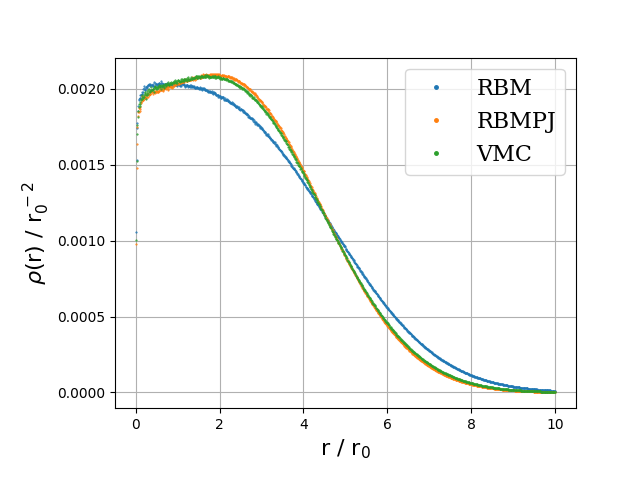
\includegraphics[width=8cm]{/home/evenmn/VMC/plots/int1/onebody/2D/2P/0.100000w/2D_2P_0p100000w_MC2pow28.png}}}
		\subfloat[6P, $\omega=0.5$]{{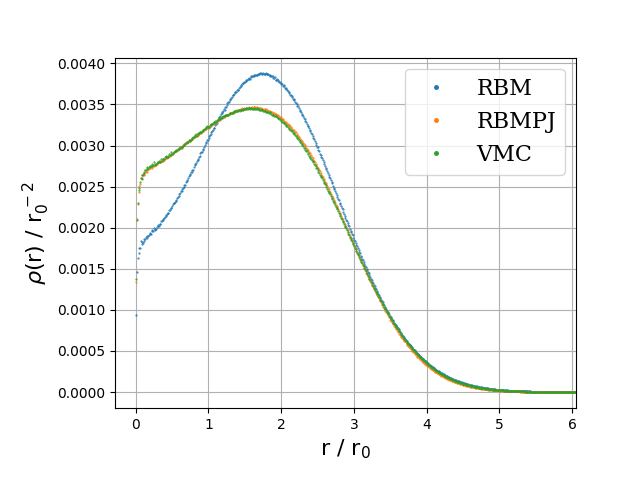
\includegraphics[width=8cm]{/home/evenmn/VMC/plots/int1/onebody/2D/6P/0.500000w/2D_6P_0p500000w_MC2pow28.png}}}
		\subfloat[6P, $\omega=1.0$]{{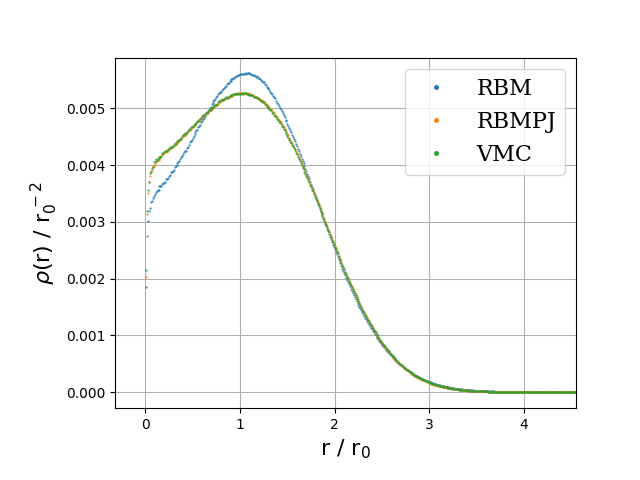
\includegraphics[width=8cm]{/home/evenmn/VMC/plots/int1/onebody/2D/6P/1.000000w/2D_6P_1p000000w_MC2pow28.png}}}
		
		\caption{One-body densities of two and six interacting electrons in two dimensions for various oscillator frequencies produced by standard variational Monte-Carlo (VMC), plain restricted Boltzmann machine (RBM) and restricted Boltzmann machine with Padé-Jastrow factor (RBMPJ). Stochastic gradient descent was used, and after convergence the number of Monte-Carlo cycles was $MC=2^{28}=268.435.456$.}%
		\label{fig:OB_interaction_2P_2D}
	\end{figure}
	\begin{figure} [H]%
		\centering
		\subfloat[12P, $\omega=0.1$]{{\includegraphics[width=8cm]{/home/evenmn/VMC/plots/int1/onebody/2D/12P/0.100000w/ADAM_MC2pow28.png}}}
		\subfloat[12P, $\omega=0.5$]{{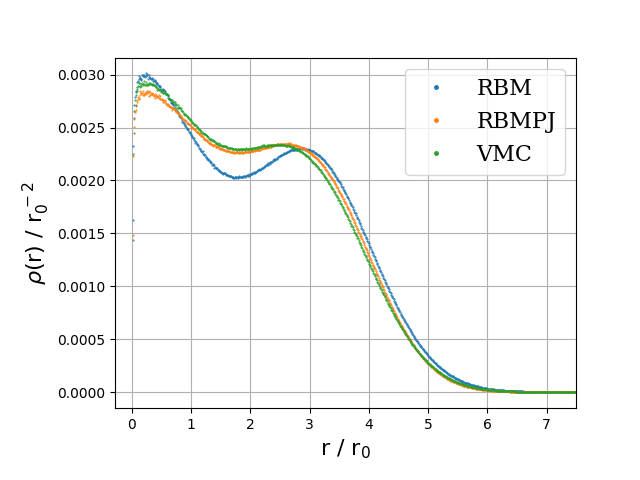
\includegraphics[width=8cm]{/home/evenmn/VMC/plots/int1/onebody/2D/12P/0.500000w/2D_12P_0p500000w_MC2pow28.png}}}
		\subfloat[12P, $\omega=1.0$]{{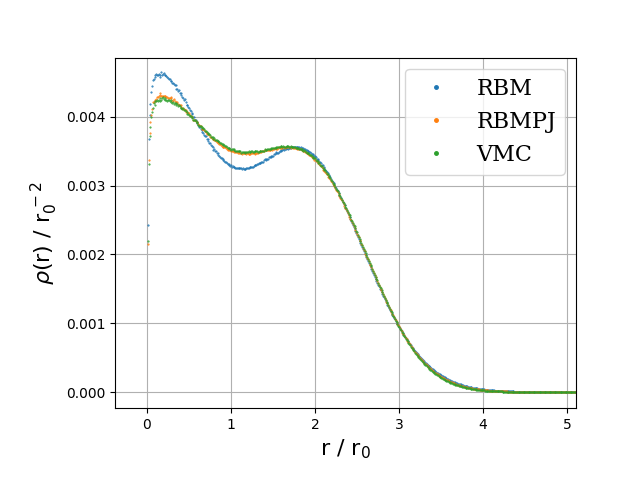
\includegraphics[width=8cm]{/home/evenmn/VMC/plots/int1/onebody/2D/12P/1.000000w/2D_12P_1p000000w_MC2pow28.png}}} \\
		
		\subfloat[20P, $\omega=0.1$]{{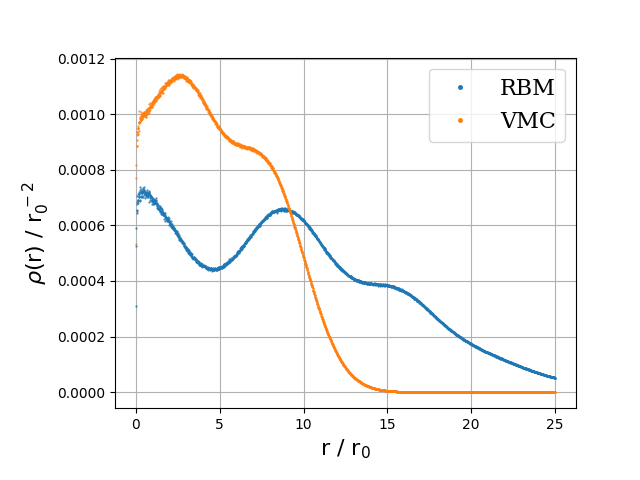
\includegraphics[width=8cm]{/home/evenmn/VMC/plots/int1/onebody/2D/20P/0.100000w/2D_20P_0p100000w_MC2pow28.png}}}
		\subfloat[20P, $\omega=0.5$]{{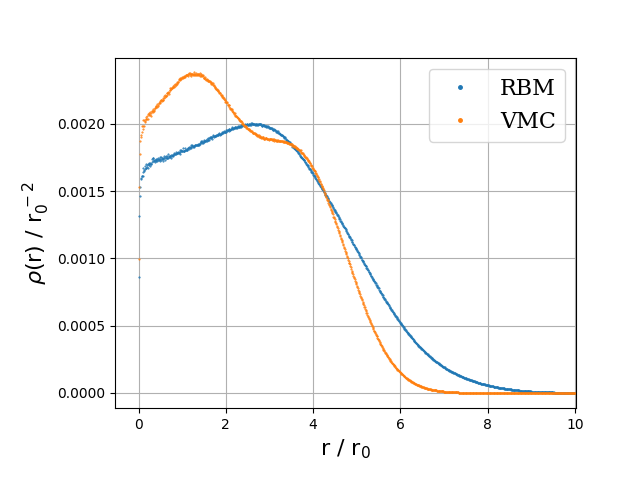
\includegraphics[width=8cm]{/home/evenmn/VMC/plots/int1/onebody/2D/20P/0.500000w/2D_20P_0p500000w_MC2pow28.png}}}
		\subfloat[20P, $\omega=1.0$]{{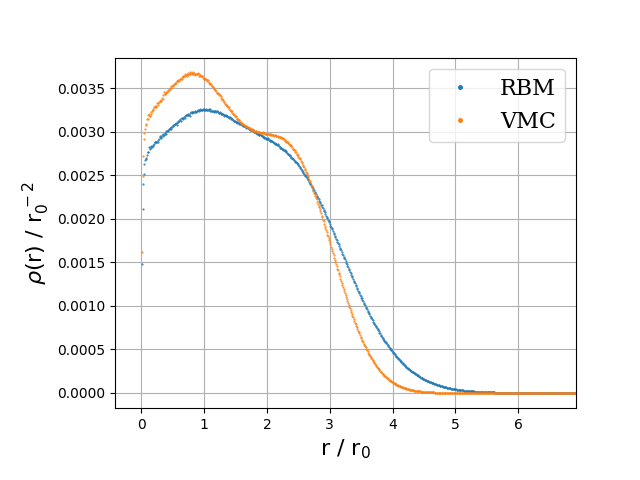
\includegraphics[width=8cm]{/home/evenmn/VMC/plots/int1/onebody/2D/20P/1.000000w/2D_20P_1p000000w_MC2pow28.png}}}
		
		\caption{One-body densities of 12 and 20 interacting electrons in two dimensions for various oscillator frequencies produced by standard variational Monte-Carlo (VMC), plain restricted Boltzmann machine (RBM) and restricted Boltzmann machine with Padé-Jastrow factor (RBMPJ). Stochastic gradient descent was used, and after convergence the number of Monte-Carlo cycles was $MC=2^{28}=268.435.456$.}%
		\label{fig:OB_interaction_12P_2D}
	\end{figure}
	
	\begin{figure} [H]%
		\centering
		\subfloat[30P, $\omega=0.1$]{{\includegraphics[width=8cm]{/home/evenmn/VMC/plots/int1/onebody/2D/30P/0.100000w/ADAM_MC2pow28.png}}}
		\subfloat[30P, $\omega=0.5$]{{\includegraphics[width=8cm]{/home/evenmn/VMC/plots/int1/onebody/2D/30P/0.500000w/ADAM_MC2pow28.png}}}
		\subfloat[30P, $\omega=1.0$]{{\includegraphics[width=8cm]{/home/evenmn/VMC/plots/int1/onebody/2D/30P/1.000000w/ADAM_MC2pow28.png}}} \\
		
		\subfloat[42P, $\omega=0.1$]{{\includegraphics[width=8cm]{/home/evenmn/VMC/plots/int1/onebody/2D/42P/0.100000w/ADAM_MC2pow28.png}}}
		\subfloat[42P, $\omega=0.5$]{{\includegraphics[width=8cm]{/home/evenmn/VMC/plots/int1/onebody/2D/42P/0.500000w/ADAM_MC2pow28.png}}}
		\subfloat[42P, $\omega=1.0$]{{\includegraphics[width=8cm]{/home/evenmn/VMC/plots/int1/onebody/2D/42P/1.000000w/ADAM_MC2pow28.png}}}
		
		\caption{One-body densities of 30 and 42 interacting electrons in two dimensions for various oscillator frequencies produced by standard variational Monte-Carlo (VMC), plain restricted Boltzmann machine (RBM) and restricted Boltzmann machine with Padé-Jastrow factor (RBMPJ). Stochastic gradient descent was used, and after convergence the number of Monte-Carlo cycles was $MC=2^{28}=268.435.456$.}%
		\label{fig:OB_interaction_30P_2D}
	\end{figure}

	\begin{figure} [H]%
		\centering
		\subfloat[56P, $\omega=0.1$]{{\includegraphics[width=8cm]{/home/evenmn/VMC/plots/int1/onebody/2D/56P/0.100000w/ADAM_MC2pow28.png}}}
		\subfloat[56P, $\omega=0.5$]{{\includegraphics[width=8cm]{/home/evenmn/VMC/plots/int1/onebody/2D/56P/0.500000w/ADAM_MC2pow28.png}}}
		\subfloat[56P, $\omega=1.0$]{{\includegraphics[width=8cm]{/home/evenmn/VMC/plots/int1/onebody/2D/56P/1.000000w/ADAM_MC2pow28.png}}} \\
		
		\subfloat[72P, $\omega=0.1$]{{\includegraphics[width=8cm]{/home/evenmn/VMC/plots/int1/onebody/2D/72P/0.100000w/ADAM_MC2pow28.png}}}
		\subfloat[72P, $\omega=0.5$]{{\includegraphics[width=8cm]{/home/evenmn/VMC/plots/int1/onebody/2D/72P/0.500000w/ADAM_MC2pow28.png}}}
		\subfloat[72P, $\omega=1.0$]{{\includegraphics[width=8cm]{/home/evenmn/VMC/plots/int1/onebody/2D/72P/1.000000w/ADAM_MC2pow28.png}}}
		
		\caption{One-body densities of 56 and 72 interacting electrons in two dimensions for various oscillator frequencies produced by standard variational Monte-Carlo (VMC), plain restricted Boltzmann machine (RBM) and restricted Boltzmann machine with Padé-Jastrow factor (RBMPJ). Stochastic gradient descent was used, and after convergence the number of Monte-Carlo cycles was $MC=2^{28}=268.435.456$.}%
		\label{fig:OB_interaction_56P_2D}
	\end{figure}
\subsubsection{Three dimensions}
\begin{figure} [H]%
	\centering
	\subfloat[2P, $\omega=0.1$]{{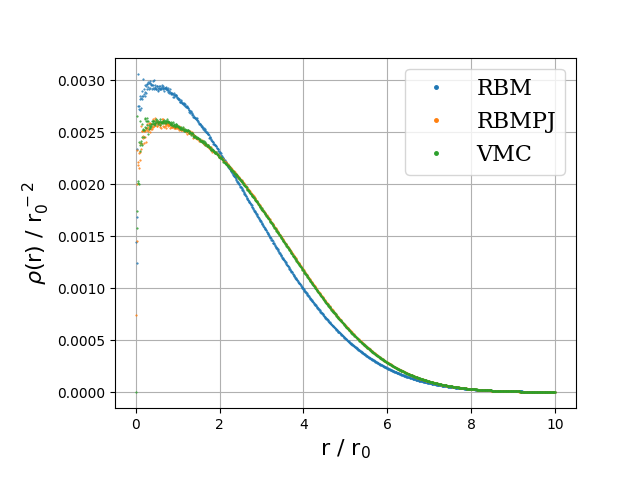
\includegraphics[width=8cm]{/home/evenmn/VMC/plots/int1/onebody/3D/2P/0.100000w/3D_2P_0p100000w_MC2pow28.png}}}
	\subfloat[2P, $\omega=0.5$]{{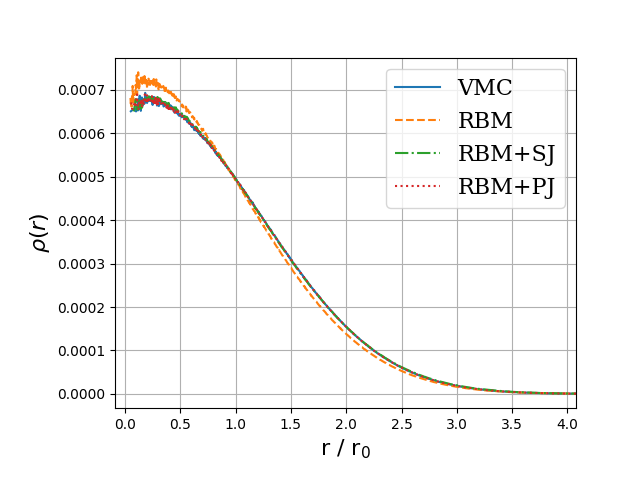
\includegraphics[width=8cm]{/home/evenmn/VMC/plots/int1/onebody/3D/2P/0.500000w/3D_2P_0p500000w_MC2pow28.png}}}
	\subfloat[2P, $\omega=1.0$]{{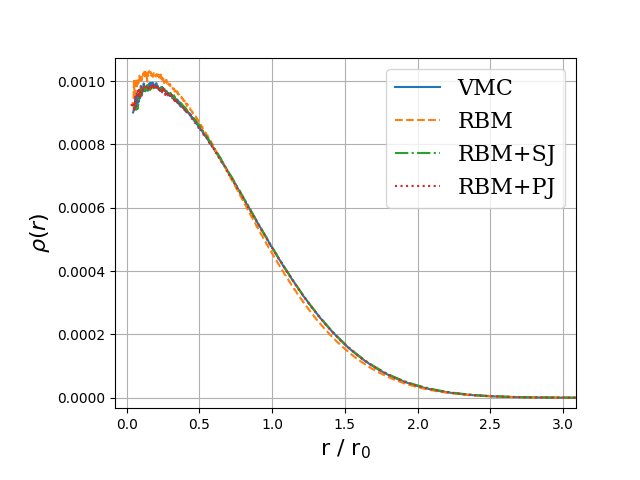
\includegraphics[width=8cm]{/home/evenmn/VMC/plots/int1/onebody/3D/2P/1.000000w/3D_2P_1p000000w_MC2pow28.png}}}\\
	
	\subfloat[8P, $\omega=0.1$]{{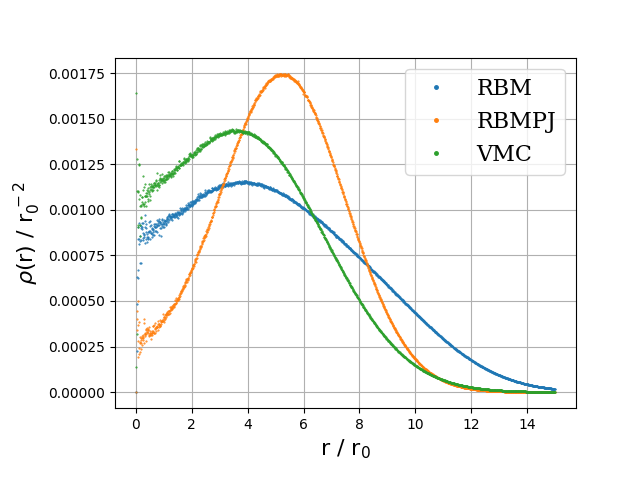
\includegraphics[width=8cm]{/home/evenmn/VMC/plots/int1/onebody/3D/8P/0.100000w/3D_8P_0p100000w_MC2pow28.png}}}
	\subfloat[8P, $\omega=0.5$]{{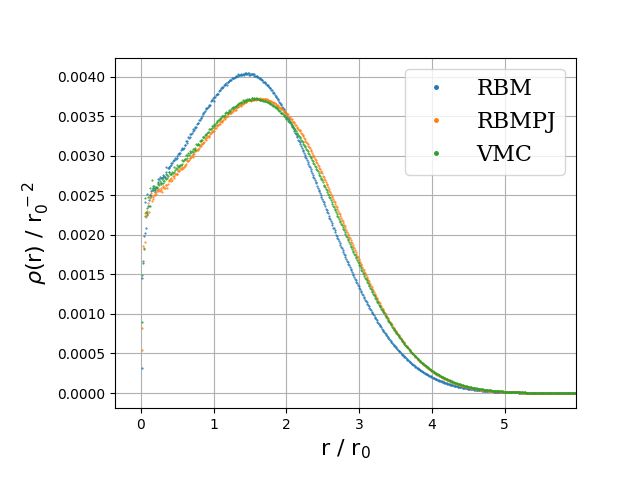
\includegraphics[width=8cm]{/home/evenmn/VMC/plots/int1/onebody/3D/8P/0.500000w/3D_8P_0p500000w_MC2pow28.png}}}
	\subfloat[8P, $\omega=1.0$]{{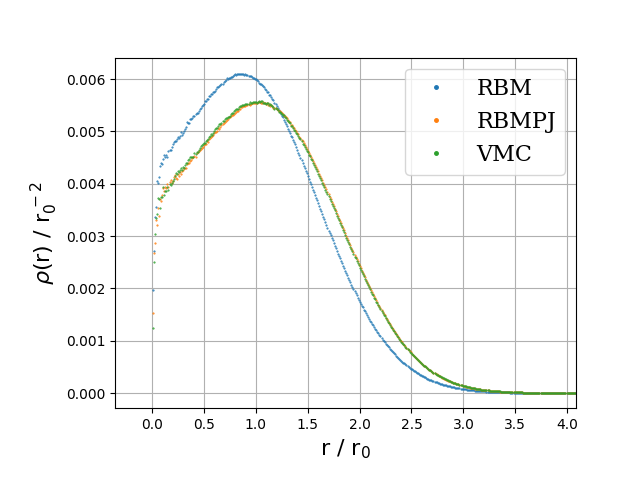
\includegraphics[width=8cm]{/home/evenmn/VMC/plots/int1/onebody/3D/8P/1.000000w/3D_8P_1p000000w_MC2pow28.png}}}
	
	\caption{One-body densities of two and eight interacting electrons in three dimensions for various oscillator frequencies produced by standard variational Monte-Carlo (VMC), plain restricted Boltzmann machine (RBM) and restricted Boltzmann machine with Padé-Jastrow factor (RBMPJ). Stochastic gradient descent was used, and after convergence the number of Monte-Carlo cycles was $MC=2^{28}=268.435.456$.}%
	\label{fig:OB_interaction_2P_3D}
\end{figure}
\begin{figure} [H]%
	\centering
	\subfloat[2P, $\omega=0.1$]{{\includegraphics[width=8cm]{/home/evenmn/VMC/plots/int1/onebody/3D/20P/0.100000w/ADAM_MC2pow28.png}}}
	\subfloat[2P, $\omega=0.5$]{{\includegraphics[width=8cm]{/home/evenmn/VMC/plots/int1/onebody/3D/20P/0.500000w/ADAM_MC2pow28.png}}}
	\subfloat[2P, $\omega=1.0$]{{\includegraphics[width=8cm]{/home/evenmn/VMC/plots/int1/onebody/3D/20P/1.000000w/ADAM_MC2pow28.png}}}\\
	
	\subfloat[8P, $\omega=0.1$]{{\includegraphics[width=8cm]{/home/evenmn/VMC/plots/int1/onebody/3D/40P/0.100000w/ADAM_MC2pow28.png}}}
	\subfloat[8P, $\omega=0.5$]{{\includegraphics[width=8cm]{/home/evenmn/VMC/plots/int1/onebody/3D/40P/0.500000w/ADAM_MC2pow28.png}}}
	\subfloat[8P, $\omega=1.0$]{{\includegraphics[width=8cm]{/home/evenmn/VMC/plots/int1/onebody/3D/40P/1.000000w/ADAM_MC2pow28.png}}}
	
	\caption{One-body densities of 20 and 40 interacting electrons in three dimensions for various oscillator frequencies produced by standard variational Monte-Carlo (VMC), plain restricted Boltzmann machine (RBM) and restricted Boltzmann machine with Padé-Jastrow factor (RBMPJ). Stochastic gradient descent was used, and after convergence the number of Monte-Carlo cycles was $MC=2^{28}=268.435.456$.}%
	\label{fig:OB_interaction_20P_3D}
\end{figure}
\end{landscape}

\subsection{Two-body density plots}
\subsubsection{Two dimensions}
\begin{figure} [H]%
	\centering
	\subfloat[RBM, 2P]{{\includegraphics[width=5cm]{/home/evenmn/VMC/plots/int1/twobody/2D/2P/0.500000w/RBM_ADAM_MC2pow28.png}}}
	\subfloat[RBM+PJ, 2P]{{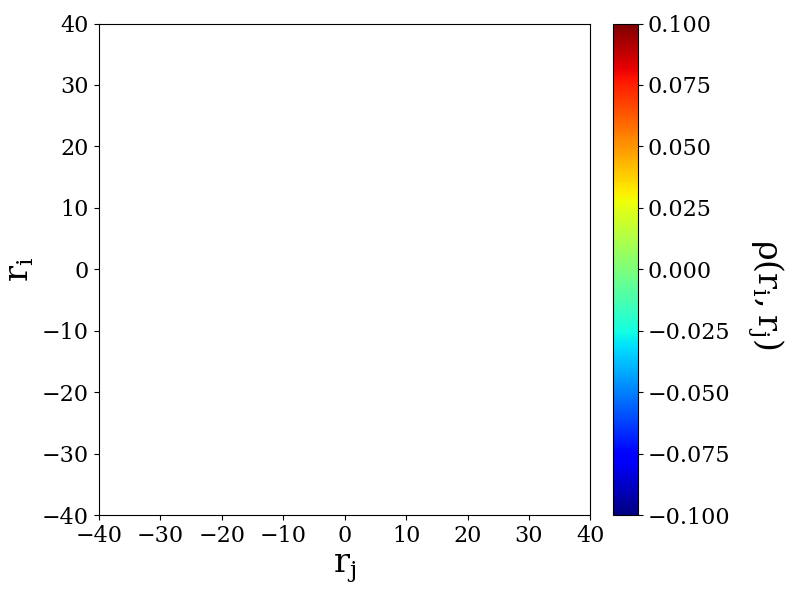
\includegraphics[width=5cm]{/home/evenmn/VMC/plots/int1/twobody/2D/2P/0.500000w/RBMPJ_ADAM_MC2pow28.png}}}
	\subfloat[VMC, 2P]{{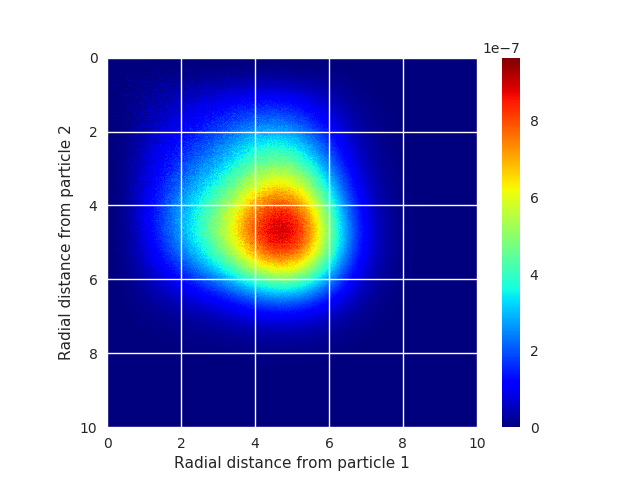
\includegraphics[width=5cm]{/home/evenmn/VMC/plots/int1/twobody/2D/2P/0.500000w/VMC_ADAM_MC2pow28.png}}}\\
	
	\subfloat[RBM, 6P]{{\includegraphics[width=5cm]{/home/evenmn/VMC/plots/int1/twobody/2D/6P/0.500000w/RBM_ADAM_MC2pow28.png}}}
	\subfloat[RBM+PJ, 6P]{{\includegraphics[width=5cm]{/home/evenmn/VMC/plots/int1/twobody/2D/6P/0.500000w/RBMPJ_ADAM_MC2pow28.png}}}
	\subfloat[VMC, 6P]{{\includegraphics[width=5cm]{/home/evenmn/VMC/plots/int1/twobody/2D/6P/0.500000w/VMC_ADAM_MC2pow28.png}}}\\
	
	\subfloat[RBM, 12P]{{\includegraphics[width=5cm]{/home/evenmn/VMC/plots/int1/twobody/2D/12P/0.500000w/RBM_ADAM_MC2pow28.png}}}
	\subfloat[RBM+PJ, 12P]{{\includegraphics[width=5cm]{/home/evenmn/VMC/plots/int1/twobody/2D/12P/0.500000w/RBMPJ_ADAM_MC2pow28.png}}}
	\subfloat[VMC, 12P]{{\includegraphics[width=5cm]{/home/evenmn/VMC/plots/int1/twobody/2D/12P/0.500000w/VMC_ADAM_MC2pow28.png}}}\\
	
	\subfloat[RBM, 20P]{{\includegraphics[width=5cm]{/home/evenmn/VMC/plots/int1/twobody/2D/20P/0.500000w/RBM_ADAM_MC2pow28.png}}}
	\subfloat[RBM+PJ, 20P]{{\includegraphics[width=4cm]{Images/example.png}}}
	\subfloat[VMC, 20P]{{\includegraphics[width=5cm]{/home/evenmn/VMC/plots/int1/twobody/2D/20P/0.500000w/VMC_ADAM_MC2pow28.png}}}
	
	\caption{Two-body densities for interacting electrons in two dimensions for $\omega=0.5$ produced by standard variational Monte-Carlo (VMC), plain restricted Boltzmann machine (RBM) and restricted Boltzmann machine with Padé-Jastrow factor (RBMPJ). ADAM optimizer was used, and after convergence the number of Monte-Carlo cycles was $MC=2^{28}=268.435.456$.}%
	\label{fig:TB_interaction_2D_1}
\end{figure}

\begin{figure} [H]%
	\centering
	\subfloat[RBM, 30P]{{\includegraphics[width=5cm]{/home/evenmn/VMC/plots/int1/twobody/2D/30P/0.500000w/RBM_ADAM_MC2pow28.png}}}
	\subfloat[RBM+PJ, 30P]{{\includegraphics[width=4cm]{Images/example.png}}}
	\subfloat[VMC, 30P]{{\includegraphics[width=5cm]{/home/evenmn/VMC/plots/int1/twobody/2D/30P/0.500000w/VMC_ADAM_MC2pow28.png}}}\\
	
	\subfloat[RBM, 42P]{{\includegraphics[width=5cm]{/home/evenmn/VMC/plots/int1/twobody/2D/42P/0.500000w/RBM_ADAM_MC2pow28.png}}}
	\subfloat[RBM+PJ, 42P]{{\includegraphics[width=4cm]{Images/example.png}}}
	\subfloat[VMC, 42P]{{\includegraphics[width=5cm]{/home/evenmn/VMC/plots/int1/twobody/2D/42P/0.500000w/VMC_ADAM_MC2pow28.png}}}\\
	
	\subfloat[RBM, 56P]{{\includegraphics[width=5cm]{/home/evenmn/VMC/plots/int1/twobody/2D/56P/0.500000w/RBM_ADAM_MC2pow28.png}}}
	\subfloat[RBM+PJ, 56P]{{\includegraphics[width=4cm]{Images/example.png}}}
	\subfloat[VMC, 56P]{{\includegraphics[width=5cm]{/home/evenmn/VMC/plots/int1/twobody/2D/56P/0.500000w/VMC_ADAM_MC2pow28.png}}}\\
	
	\subfloat[RBM, 72P]{{\includegraphics[width=5cm]{/home/evenmn/VMC/plots/int1/twobody/2D/72P/0.500000w/RBM_ADAM_MC2pow28.png}}}
	\subfloat[RBM+PJ, 72P]{{\includegraphics[width=4cm]{Images/example.png}}}
	\subfloat[VMC, 72P]{{\includegraphics[width=5cm]{/home/evenmn/VMC/plots/int1/twobody/2D/72P/0.500000w/VMC_ADAM_MC2pow28.png}}}
	
	\caption{Two-body densities for interacting electrons in two dimensions for various oscillator frequencies produced by standard variational Monte-Carlo (VMC), plain restricted Boltzmann machine (RBM) and restricted Boltzmann machine with Padé-Jastrow factor (RBMPJ). ADAM optimizer was used, and after convergence the number of Monte-Carlo cycles was $MC=2^{28}=268.435.456$.}%
	\label{fig:TB_interaction_2D_2}
\end{figure}

\subsubsection{Three dimensions}
\begin{figure} [H]%
	\centering
	\subfloat[2P, RBM]{{\includegraphics[width=5cm]{/home/evenmn/VMC/plots/int1/twobody/3D/2P/0.500000w/RBM_ADAM_MC2pow28.png}}}
	\subfloat[2P, RBM+PJ]{{\includegraphics[width=4cm]{Images/example.png}}}
	\subfloat[2P, VMC]{{\includegraphics[width=5cm]{/home/evenmn/VMC/plots/int1/twobody/3D/2P/0.500000w/VMC_ADAM_MC2pow28.png}}}\\
	
	\subfloat[8P, RBM]{{\includegraphics[width=5cm]{/home/evenmn/VMC/plots/int1/twobody/3D/8P/0.500000w/RBM_ADAM_MC2pow28.png}}}
	\subfloat[8P, RBM+PJ]{{\includegraphics[width=4cm]{Images/example.png}}}
	\subfloat[8P, VMC]{{\includegraphics[width=5cm]{/home/evenmn/VMC/plots/int1/twobody/3D/8P/0.500000w/VMC_ADAM_MC2pow28.png}}}\\
	
	\subfloat[20P, RBM]{{\includegraphics[width=5cm]{/home/evenmn/VMC/plots/int1/twobody/3D/20P/0.500000w/RBM_ADAM_MC2pow28.png}}}
	\subfloat[20P, RBM+PJ]{{\includegraphics[width=4cm]{Images/example.png}}}
	\subfloat[20P, VMC]{{\includegraphics[width=5cm]{/home/evenmn/VMC/plots/int1/twobody/3D/20P/0.500000w/VMC_ADAM_MC2pow28.png}}}\\
	
	\subfloat[40P, RBM]{{\includegraphics[width=5cm]{/home/evenmn/VMC/plots/int1/twobody/3D/40P/0.500000w/RBM_ADAM_MC2pow28.png}}}
	\subfloat[40P, RBM+PJ]{{\includegraphics[width=4cm]{Images/example.png}}}
	\subfloat[40P, VMC]{{\includegraphics[width=5cm]{/home/evenmn/VMC/plots/int1/twobody/3D/40P/0.500000w/VMC_ADAM_MC2pow28.png}}}\\
	
	\subfloat[70P, RBM]{{\includegraphics[width=5cm]{/home/evenmn/VMC/plots/int1/twobody/3D/70P/0.500000w/RBM_ADAM_MC2pow28.png}}}
	\subfloat[70P, RBM+PJ]{{\includegraphics[width=4cm]{Images/example.png}}}
	\subfloat[70P, VMC]{{\includegraphics[width=5cm]{/home/evenmn/VMC/plots/int1/twobody/3D/70P/0.500000w/VMC_ADAM_MC2pow28.png}}}
	
	\caption{Two-body densities for 72 interacting electrons in two dimensions for various oscillator frequencies produced by standard variational Monte-Carlo (VMC), plain restricted Boltzmann machine (RBM) and restricted Boltzmann machine with Padé-Jastrow factor (RBMPJ). ADAM optimizer was used, and after convergence the number of Monte-Carlo cycles was $MC=2^{28}=268.435.456$.}%
	\label{fig:TB_interaction_3D}
\end{figure}